\section{Beam Line and Detectors}
\label{hptpcPaper:sec:Methods}

    \subsection{Beam Test Overview}
    The beam test took place in the T10 beam line, East Area at the Proton Synchrotron in CERN from the 15th August to the 18th September 2018.
    The results in this paper use data taken on the 31st August and 1st September, during which the setup configuration was varied as described below.
    The primary components of the  experimental setup for the data taking period is shown in Figure~\ref{fig:setup}.
    \begin{figure}
    \includegraphics[width=1.0\linewidth]{files/Figures/T10Diagram.jpg}
    	\caption{Beam test configuration}
    		\label{fig:setup}
    \end{figure}
    The centre of the HPTPC Prototype was placed 13~m from the wire chamber, labeled as $WC$, at the beam entrance. Three ToF constituents, labeled $S1$ to $S3$, were placed upstream of the TPC, while the fourth, labeled $S4$, was placed directly downstream. Both the TPC and ToF systems were placed at an off-axis angle with respect to the direction of the beam.
    Additionally, a variable number of blocks of acrylic moderator, shown in Figure~\ref{fig:modblocks}, were placed in the beamline, immediately behind of $S1$.
    
    
    Data acquisition (DAQ) of up- and downstream ToF systems were completely independent. Due to low intensity of the beam, the synchronization between systems was done offline using the reference signal from PS at the beginning of every spill. The trigger condition of the upstream ToF was based on the coincidence between $S1$ and $S3$ constituents. While DAQ of the downstream ToF, $S4$, was run in self-triggering mode with a gate open during the spill. Coincidence signals between $S1$ and $S2$ counters was also recorded by the DAQ of the downstream ToF and was used in the particle identification (PID) analysis. 
    
    
    A system of moderator blocks was located between $S1$ and $S2$ counters.  The system is composed of a stand on which up to four polystyrene $10\times10\times10$~cm$^3$ blocks can be placed. Figure~\ref{fig:modblocks} shows the stand with four blocks on it. The moderator blocks have the effect of both reducing the energy of incoming particles as well as scattering protons at higher angles than minimum ionizing particles (MIP), thus increasing the proton to MIP ratio at off-axis angles from the beam. 
    
    Data was taken with the beam momentum primarily at 0.8~GeV/c, and with each configuration of 0 to 4 moderator blocks. Figure~INSERT shows the typical composition of the beam upstream of $S1$ at 0.8~GeV/c. Beam spills are approximately 500~ms in length with 5-10~s between spills.  
    
%    Moderator blocks were used in order to cause a spread in the incoming beam.
%    The blocks cause protons to scatter through a larger angle than pions and other minimum ionising particles (MIP), increasing the off-axis proton pion ratio.
%    The effect of this, together with placing the TPC and ToF systems off axis was to allow a measurement of protons with a lower pion background.
%    This technique also had the effect of reducing the average momentum of the measured particles.
%    Data were taken for 0, 1, 2, 3, and 4 moderator blocks in turn.
%    The beam ran with an energy of 0.8~GeV/c, and primarily comprised protons and pions, as well as muons and electrons. 
%    Beam spills were approximately 500~ms in length, with 5-10~s between spills.
%    The ratio of protons to pions expected in the T10 beam  is shown in figure~\ref{beamcharacteristics}.
%    From this figure, the expected on axis proton pion ratio at 0.8~GeV/c is approximately 1:6.
%      \begin{figure}
%      \centering
%    \includegraphics[width=0.6\linewidth]{files/Figures/offaxismeasurement.png}
%    	\caption{T10 beam constituents (REFERENCE NEEDED)}
%    		\label{fig:beamcharacteristics}
%    \end{figure}
    
    
    \begin{figure}[t]
      \centering
    %\includegraphics[width=0.2\linewidth]{files/Figures/ModeratorBlocks.jpg}
    \includegraphics[width=1.05\linewidth]{files/Figures/S1S2S3S4.png}
    	\caption{Photo demonstrating the $S1$ and $S2$ counters and the stand with four acrylic moderator blocks of the upstream part of the setup (right). Photo of the downstream part of the setup which shows the $S3$, $S4$ detectors and HPTPC (left).}
    		\label{fig:modblocks}
    \end{figure}
    
    
	\subsection{Upstream beam counters $S1$ and $S2$}
	
	The beam counters $S1$ and $S2$ are shown in Figure~\ref{fig:modblocks}. The $S1$ counter is a $40\times40\times5$~mm$^3$ plastic scintillator tile which is attached to four 1'' Hamamatsu R4998 phototubes from four ends for the light readout. The time resolution of the counter, as measured by the DAQ system of the upstream ToF, was about 30~ps. 
	
	The counter $S2$ was placed 1.4~m (TBC) downstream of $S1$. The size of the scintillator tile, $120\times120\times5$~mm$^3$, and its position were adjusted to account for the beam divergence in the moderator blocks. The light was collected by a 2'' PMT R13089 which was connected to the scintillator via long light-guide as shown in Figure~\ref{fig:modblocks}. 
	
	The analog signals from one of the $S1$ PMTs and $S2$ PMT were fed into NIM discriminator units.
	%set at AA mV and BB mV respectively. 
	As a next step, the discriminated signals were fed into a NIM coincidence unit, and the coincidence of the two signals was recorded by the DAQ systems of $S3$ and $S4$. This information was further used for the time-of-flight analysis of the downstream ToF. 

    
\subsection{Upstream Time of Flight instrumentation ($S3$)}

The $S3$ `upstream' ToF constituent sits just upstream of the HPTPC prototype in the beamline. The sketch of the $S3$ ToF constituent is shown in Figure~\ref{fig:S3sketch}. The detector is composed of 22 staggered bars:  20 bars with dimensions $1.68 \times 6 \times 1$~cm$^3$ and 2 bars of  $1.5 \times 6 \times 1$~cm$^3$ placed on top and bottom \cite{S3-proceedings}.
The overlap between bars was set to 5~mm, thus the active area of the detector was approximately 1.68~m $\times$ 1.22~m.
     \begin{figure}
      \centering
    \includegraphics[width=0.7\linewidth]{files/Figures/uToF_sketch.pdf}
    	\caption{Sketch of the $S3$ wall \cite{S3-proceedings}.}
    		\label{fig:S3sketch}
    \end{figure}
    
The bars are made from the plastic EJ-200 \cite{SCIONIX}, which 
provides a suitable optical attenuation length 4~m and fast timing (rise time of 0.9~ns and decay time 2.1~ns). 
The scintillation emission spectrum of EJ-200 resides primarily in the violet region of the visible spectrum that well corresponds to the maximum absorption region of photosensors used for the readout.

Arrays of eight $6 \times 6$~mm$^2$ area silicone photomultipliers (SiPMs) S13360-6050PE from Hamamatsu Photonics \cite{Hamamatsu} were coupled to both ends of the bar to collect scintillation photons. Anode signals of SiPMs have been read out, summed and shaped by a dedicated circuit as described in Ref.\,\cite{S3-readout}.
%an 8-channel SiPM anode readout integrated circuit MUSIC-R1. %The construction of the prototype was a joint effort between groups of Geneva and Zurich universities as a part of R\&D for the Timing detector of the SHIP experiment \cite{AK}.

A 64-ch SAMPIC  module was used for the data acquisition. A SAMPIC chip is a Waveform and Time to Digital Converter (WTDC) 16-channel ASIC which provides a raw time with an ultrafast analog memory allowing fine timing extraction as well as other parameters of the pulse~\cite{SAMPIC}. Each channel integrates a discriminator that can trigger itself independently or participate to a more complex trigger. 
Three ASICs ($16\times3=48$ channels) of the module were connected to 44 channels of $S3$ and were run in self-triggering mode. The 4th ASIC was used to acquire data from $S1$, coincidence signal $S1\cap S2$ and the start-of-spill signal from PS. A second level trigger was implemented in firmware and run on a level of ASICs. 
Namely, the data were sent to the hard disk of the DAQ notebook only in the case of coincidence between $S1$ channels and channels of three ASICs used for $S3$.


A mean time of light signals detected at two ends of a single bar provides a time reference with the resolution of about 100~ps, while the difference between the time of the light signals gives the position of the interaction along the bar, with a resolution of 1.6~cm. Examples of reconstructed $XY$ distributions are shown in Figures~\ref{fig:s3XY_pion} and~\ref{fig:s3XY_proton}.



\begin{figure}[t]
	\begin{minipage}[t]{0.49\textwidth}
		\centering
		\begin{adjustbox}{max totalsize={\textwidth}{.5\textheight},center}
			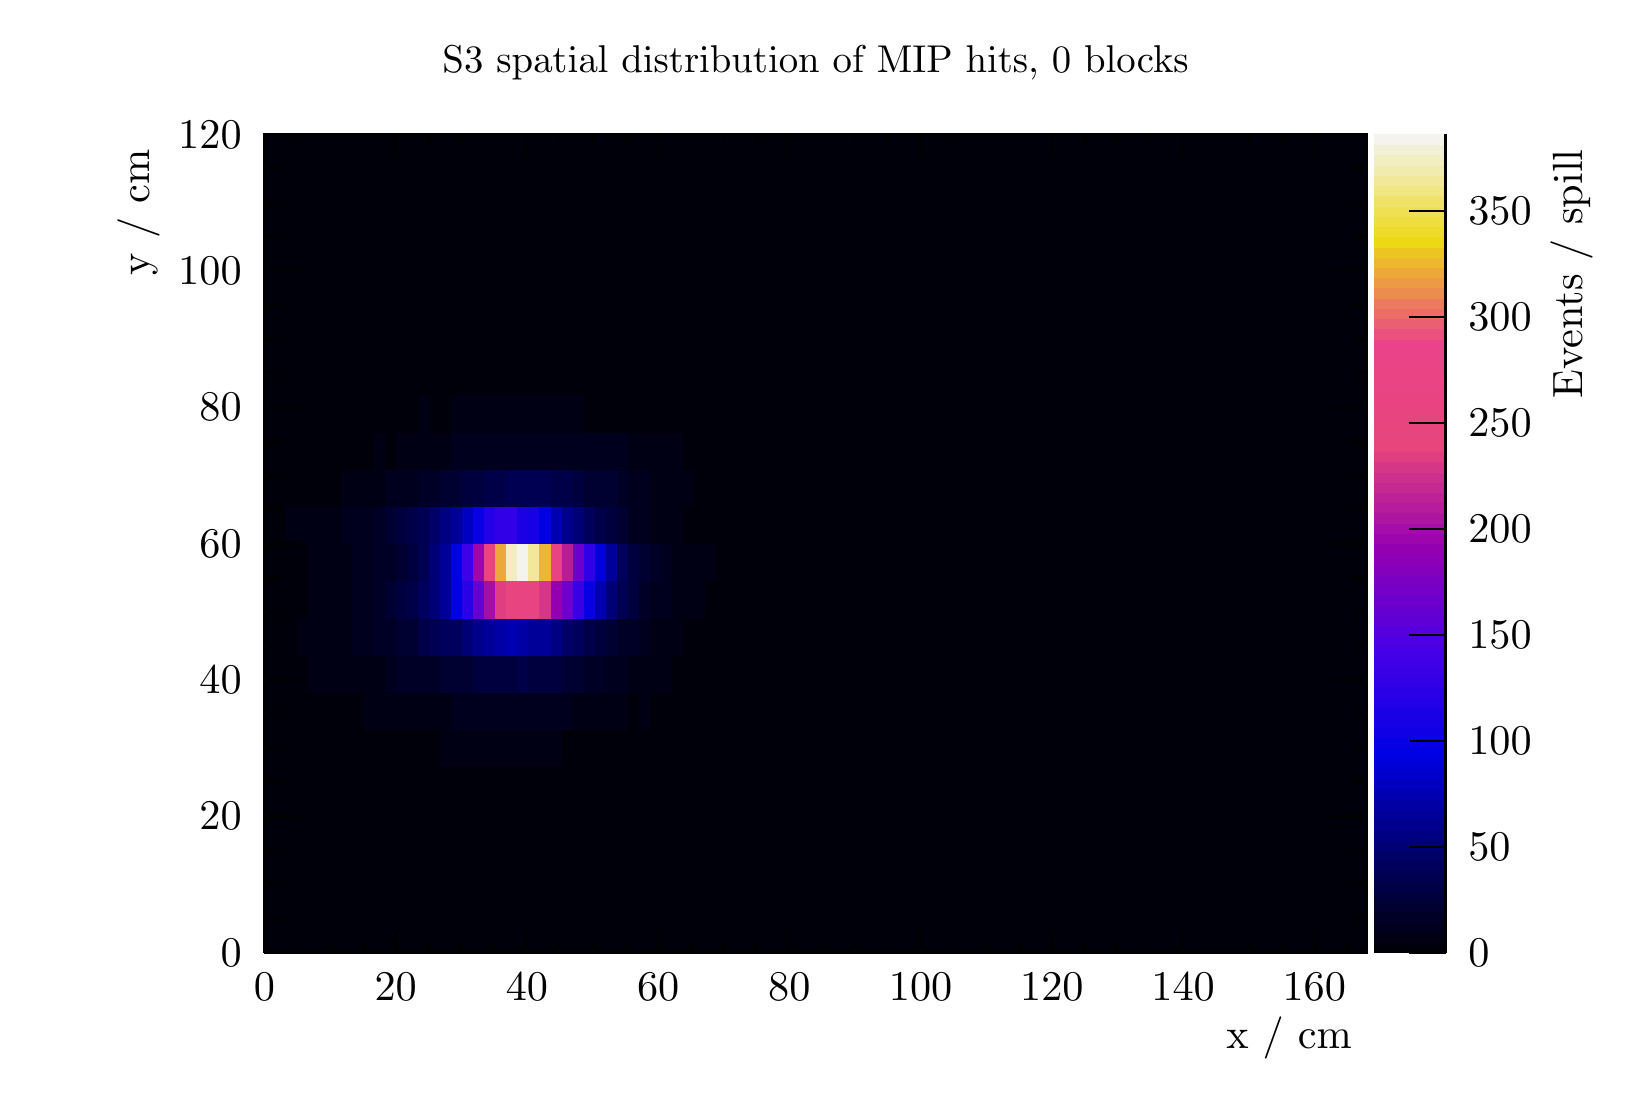
\begin{tikzpicture}
\pgfdeclareplotmark{cross} {
\pgfpathmoveto{\pgfpoint{-0.3\pgfplotmarksize}{\pgfplotmarksize}}
\pgfpathlineto{\pgfpoint{+0.3\pgfplotmarksize}{\pgfplotmarksize}}
\pgfpathlineto{\pgfpoint{+0.3\pgfplotmarksize}{0.3\pgfplotmarksize}}
\pgfpathlineto{\pgfpoint{+1\pgfplotmarksize}{0.3\pgfplotmarksize}}
\pgfpathlineto{\pgfpoint{+1\pgfplotmarksize}{-0.3\pgfplotmarksize}}
\pgfpathlineto{\pgfpoint{+0.3\pgfplotmarksize}{-0.3\pgfplotmarksize}}
\pgfpathlineto{\pgfpoint{+0.3\pgfplotmarksize}{-1.\pgfplotmarksize}}
\pgfpathlineto{\pgfpoint{-0.3\pgfplotmarksize}{-1.\pgfplotmarksize}}
\pgfpathlineto{\pgfpoint{-0.3\pgfplotmarksize}{-0.3\pgfplotmarksize}}
\pgfpathlineto{\pgfpoint{-1.\pgfplotmarksize}{-0.3\pgfplotmarksize}}
\pgfpathlineto{\pgfpoint{-1.\pgfplotmarksize}{0.3\pgfplotmarksize}}
\pgfpathlineto{\pgfpoint{-0.3\pgfplotmarksize}{0.3\pgfplotmarksize}}
\pgfpathclose
\pgfusepathqstroke
}
\pgfdeclareplotmark{cross*} {
\pgfpathmoveto{\pgfpoint{-0.3\pgfplotmarksize}{\pgfplotmarksize}}
\pgfpathlineto{\pgfpoint{+0.3\pgfplotmarksize}{\pgfplotmarksize}}
\pgfpathlineto{\pgfpoint{+0.3\pgfplotmarksize}{0.3\pgfplotmarksize}}
\pgfpathlineto{\pgfpoint{+1\pgfplotmarksize}{0.3\pgfplotmarksize}}
\pgfpathlineto{\pgfpoint{+1\pgfplotmarksize}{-0.3\pgfplotmarksize}}
\pgfpathlineto{\pgfpoint{+0.3\pgfplotmarksize}{-0.3\pgfplotmarksize}}
\pgfpathlineto{\pgfpoint{+0.3\pgfplotmarksize}{-1.\pgfplotmarksize}}
\pgfpathlineto{\pgfpoint{-0.3\pgfplotmarksize}{-1.\pgfplotmarksize}}
\pgfpathlineto{\pgfpoint{-0.3\pgfplotmarksize}{-0.3\pgfplotmarksize}}
\pgfpathlineto{\pgfpoint{-1.\pgfplotmarksize}{-0.3\pgfplotmarksize}}
\pgfpathlineto{\pgfpoint{-1.\pgfplotmarksize}{0.3\pgfplotmarksize}}
\pgfpathlineto{\pgfpoint{-0.3\pgfplotmarksize}{0.3\pgfplotmarksize}}
\pgfpathclose
\pgfusepathqfillstroke
}
\pgfdeclareplotmark{newstar} {
\pgfpathmoveto{\pgfqpoint{0pt}{\pgfplotmarksize}}
\pgfpathlineto{\pgfqpointpolar{44}{0.5\pgfplotmarksize}}
\pgfpathlineto{\pgfqpointpolar{18}{\pgfplotmarksize}}
\pgfpathlineto{\pgfqpointpolar{-20}{0.5\pgfplotmarksize}}
\pgfpathlineto{\pgfqpointpolar{-54}{\pgfplotmarksize}}
\pgfpathlineto{\pgfqpointpolar{-90}{0.5\pgfplotmarksize}}
\pgfpathlineto{\pgfqpointpolar{234}{\pgfplotmarksize}}
\pgfpathlineto{\pgfqpointpolar{198}{0.5\pgfplotmarksize}}
\pgfpathlineto{\pgfqpointpolar{162}{\pgfplotmarksize}}
\pgfpathlineto{\pgfqpointpolar{134}{0.5\pgfplotmarksize}}
\pgfpathclose
\pgfusepathqstroke
}
\pgfdeclareplotmark{newstar*} {
\pgfpathmoveto{\pgfqpoint{0pt}{\pgfplotmarksize}}
\pgfpathlineto{\pgfqpointpolar{44}{0.5\pgfplotmarksize}}
\pgfpathlineto{\pgfqpointpolar{18}{\pgfplotmarksize}}
\pgfpathlineto{\pgfqpointpolar{-20}{0.5\pgfplotmarksize}}
\pgfpathlineto{\pgfqpointpolar{-54}{\pgfplotmarksize}}
\pgfpathlineto{\pgfqpointpolar{-90}{0.5\pgfplotmarksize}}
\pgfpathlineto{\pgfqpointpolar{234}{\pgfplotmarksize}}
\pgfpathlineto{\pgfqpointpolar{198}{0.5\pgfplotmarksize}}
\pgfpathlineto{\pgfqpointpolar{162}{\pgfplotmarksize}}
\pgfpathlineto{\pgfqpointpolar{134}{0.5\pgfplotmarksize}}
\pgfpathclose
\pgfusepathqfillstroke
}
\definecolor{c}{rgb}{1,1,1};
\draw [color=c, fill=c] (0,0) rectangle (20,13.4957);
\draw [color=c, fill=c] (3,1.75444) rectangle (17,12.1461);
\definecolor{c}{rgb}{0,0,0};
\draw [c,line width=0.9] (3,1.75444) -- (3,12.1461) -- (17,12.1461) -- (17,1.75444) -- (3,1.75444);
\definecolor{c}{rgb}{1,1,1};
\draw [color=c, fill=c] (3,1.75444) rectangle (17,12.1461);
\definecolor{c}{rgb}{0,0,0};
\draw [c,line width=0.9] (3,1.75444) -- (3,12.1461) -- (17,12.1461) -- (17,1.75444) -- (3,1.75444);
\definecolor{c}{rgb}{0,0,0.0387097};
\draw [color=c, fill=c] (3,1.75444) rectangle (3.14,2.22679);
\draw [color=c, fill=c] (3.14,1.75444) rectangle (3.28,2.22679);
\draw [color=c, fill=c] (3.28,1.75444) rectangle (3.42,2.22679);
\draw [color=c, fill=c] (3.42,1.75444) rectangle (3.56,2.22679);
\draw [color=c, fill=c] (3.56,1.75444) rectangle (3.7,2.22679);
\draw [color=c, fill=c] (3.7,1.75444) rectangle (3.84,2.22679);
\draw [color=c, fill=c] (3.84,1.75444) rectangle (3.98,2.22679);
\draw [color=c, fill=c] (3.98,1.75444) rectangle (4.12,2.22679);
\draw [color=c, fill=c] (4.12,1.75444) rectangle (4.26,2.22679);
\draw [color=c, fill=c] (4.26,1.75444) rectangle (4.4,2.22679);
\draw [color=c, fill=c] (4.4,1.75444) rectangle (4.54,2.22679);
\draw [color=c, fill=c] (4.54,1.75444) rectangle (4.68,2.22679);
\draw [color=c, fill=c] (4.68,1.75444) rectangle (4.82,2.22679);
\draw [color=c, fill=c] (4.82,1.75444) rectangle (4.96,2.22679);
\draw [color=c, fill=c] (4.96,1.75444) rectangle (5.1,2.22679);
\draw [color=c, fill=c] (5.1,1.75444) rectangle (5.24,2.22679);
\draw [color=c, fill=c] (5.24,1.75444) rectangle (5.38,2.22679);
\draw [color=c, fill=c] (5.38,1.75444) rectangle (5.52,2.22679);
\draw [color=c, fill=c] (5.52,1.75444) rectangle (5.66,2.22679);
\draw [color=c, fill=c] (5.66,1.75444) rectangle (5.8,2.22679);
\draw [color=c, fill=c] (5.8,1.75444) rectangle (5.94,2.22679);
\draw [color=c, fill=c] (5.94,1.75444) rectangle (6.08,2.22679);
\draw [color=c, fill=c] (6.08,1.75444) rectangle (6.22,2.22679);
\draw [color=c, fill=c] (6.22,1.75444) rectangle (6.36,2.22679);
\draw [color=c, fill=c] (6.36,1.75444) rectangle (6.5,2.22679);
\draw [color=c, fill=c] (6.5,1.75444) rectangle (6.64,2.22679);
\draw [color=c, fill=c] (6.64,1.75444) rectangle (6.78,2.22679);
\draw [color=c, fill=c] (6.78,1.75444) rectangle (6.92,2.22679);
\draw [color=c, fill=c] (6.92,1.75444) rectangle (7.06,2.22679);
\draw [color=c, fill=c] (7.06,1.75444) rectangle (7.2,2.22679);
\draw [color=c, fill=c] (7.2,1.75444) rectangle (7.34,2.22679);
\draw [color=c, fill=c] (7.34,1.75444) rectangle (7.48,2.22679);
\draw [color=c, fill=c] (7.48,1.75444) rectangle (7.62,2.22679);
\draw [color=c, fill=c] (7.62,1.75444) rectangle (7.76,2.22679);
\draw [color=c, fill=c] (7.76,1.75444) rectangle (7.9,2.22679);
\draw [color=c, fill=c] (7.9,1.75444) rectangle (8.04,2.22679);
\draw [color=c, fill=c] (8.04,1.75444) rectangle (8.18,2.22679);
\draw [color=c, fill=c] (8.18,1.75444) rectangle (8.32,2.22679);
\draw [color=c, fill=c] (8.32,1.75444) rectangle (8.46,2.22679);
\draw [color=c, fill=c] (8.46,1.75444) rectangle (8.6,2.22679);
\draw [color=c, fill=c] (8.6,1.75444) rectangle (8.74,2.22679);
\draw [color=c, fill=c] (8.74,1.75444) rectangle (8.88,2.22679);
\draw [color=c, fill=c] (8.88,1.75444) rectangle (9.02,2.22679);
\draw [color=c, fill=c] (9.02,1.75444) rectangle (9.16,2.22679);
\draw [color=c, fill=c] (9.16,1.75444) rectangle (9.3,2.22679);
\draw [color=c, fill=c] (9.3,1.75444) rectangle (9.44,2.22679);
\draw [color=c, fill=c] (9.44,1.75444) rectangle (9.58,2.22679);
\draw [color=c, fill=c] (9.58,1.75444) rectangle (9.72,2.22679);
\draw [color=c, fill=c] (9.72,1.75444) rectangle (9.86,2.22679);
\draw [color=c, fill=c] (9.86,1.75444) rectangle (10,2.22679);
\draw [color=c, fill=c] (10,1.75444) rectangle (10.14,2.22679);
\draw [color=c, fill=c] (10.14,1.75444) rectangle (10.28,2.22679);
\draw [color=c, fill=c] (10.28,1.75444) rectangle (10.42,2.22679);
\draw [color=c, fill=c] (10.42,1.75444) rectangle (10.56,2.22679);
\draw [color=c, fill=c] (10.56,1.75444) rectangle (10.7,2.22679);
\draw [color=c, fill=c] (10.7,1.75444) rectangle (10.84,2.22679);
\draw [color=c, fill=c] (10.84,1.75444) rectangle (10.98,2.22679);
\draw [color=c, fill=c] (10.98,1.75444) rectangle (11.12,2.22679);
\draw [color=c, fill=c] (11.12,1.75444) rectangle (11.26,2.22679);
\draw [color=c, fill=c] (11.26,1.75444) rectangle (11.4,2.22679);
\draw [color=c, fill=c] (11.4,1.75444) rectangle (11.54,2.22679);
\draw [color=c, fill=c] (11.54,1.75444) rectangle (11.68,2.22679);
\draw [color=c, fill=c] (11.68,1.75444) rectangle (11.82,2.22679);
\draw [color=c, fill=c] (11.82,1.75444) rectangle (11.96,2.22679);
\draw [color=c, fill=c] (11.96,1.75444) rectangle (12.1,2.22679);
\draw [color=c, fill=c] (12.1,1.75444) rectangle (12.24,2.22679);
\draw [color=c, fill=c] (12.24,1.75444) rectangle (12.38,2.22679);
\draw [color=c, fill=c] (12.38,1.75444) rectangle (12.52,2.22679);
\draw [color=c, fill=c] (12.52,1.75444) rectangle (12.66,2.22679);
\draw [color=c, fill=c] (12.66,1.75444) rectangle (12.8,2.22679);
\draw [color=c, fill=c] (12.8,1.75444) rectangle (12.94,2.22679);
\draw [color=c, fill=c] (12.94,1.75444) rectangle (13.08,2.22679);
\draw [color=c, fill=c] (13.08,1.75444) rectangle (13.22,2.22679);
\draw [color=c, fill=c] (13.22,1.75444) rectangle (13.36,2.22679);
\draw [color=c, fill=c] (13.36,1.75444) rectangle (13.5,2.22679);
\draw [color=c, fill=c] (13.5,1.75444) rectangle (13.64,2.22679);
\draw [color=c, fill=c] (13.64,1.75444) rectangle (13.78,2.22679);
\draw [color=c, fill=c] (13.78,1.75444) rectangle (13.92,2.22679);
\draw [color=c, fill=c] (13.92,1.75444) rectangle (14.06,2.22679);
\draw [color=c, fill=c] (14.06,1.75444) rectangle (14.2,2.22679);
\draw [color=c, fill=c] (14.2,1.75444) rectangle (14.34,2.22679);
\draw [color=c, fill=c] (14.34,1.75444) rectangle (14.48,2.22679);
\draw [color=c, fill=c] (14.48,1.75444) rectangle (14.62,2.22679);
\draw [color=c, fill=c] (14.62,1.75444) rectangle (14.76,2.22679);
\draw [color=c, fill=c] (14.76,1.75444) rectangle (14.9,2.22679);
\draw [color=c, fill=c] (14.9,1.75444) rectangle (15.04,2.22679);
\draw [color=c, fill=c] (15.04,1.75444) rectangle (15.18,2.22679);
\draw [color=c, fill=c] (15.18,1.75444) rectangle (15.32,2.22679);
\draw [color=c, fill=c] (15.32,1.75444) rectangle (15.46,2.22679);
\draw [color=c, fill=c] (15.46,1.75444) rectangle (15.6,2.22679);
\draw [color=c, fill=c] (15.6,1.75444) rectangle (15.74,2.22679);
\draw [color=c, fill=c] (15.74,1.75444) rectangle (15.88,2.22679);
\draw [color=c, fill=c] (15.88,1.75444) rectangle (16.02,2.22679);
\draw [color=c, fill=c] (16.02,1.75444) rectangle (16.16,2.22679);
\draw [color=c, fill=c] (16.16,1.75444) rectangle (16.3,2.22679);
\draw [color=c, fill=c] (16.3,1.75444) rectangle (16.44,2.22679);
\draw [color=c, fill=c] (16.44,1.75444) rectangle (16.58,2.22679);
\draw [color=c, fill=c] (16.58,1.75444) rectangle (16.72,2.22679);
\draw [color=c, fill=c] (16.72,1.75444) rectangle (16.86,2.22679);
\draw [color=c, fill=c] (16.86,1.75444) rectangle (17,2.22679);
\draw [color=c, fill=c] (3,2.22679) rectangle (3.14,2.69914);
\draw [color=c, fill=c] (3.14,2.22679) rectangle (3.28,2.69914);
\draw [color=c, fill=c] (3.28,2.22679) rectangle (3.42,2.69914);
\draw [color=c, fill=c] (3.42,2.22679) rectangle (3.56,2.69914);
\draw [color=c, fill=c] (3.56,2.22679) rectangle (3.7,2.69914);
\draw [color=c, fill=c] (3.7,2.22679) rectangle (3.84,2.69914);
\draw [color=c, fill=c] (3.84,2.22679) rectangle (3.98,2.69914);
\draw [color=c, fill=c] (3.98,2.22679) rectangle (4.12,2.69914);
\draw [color=c, fill=c] (4.12,2.22679) rectangle (4.26,2.69914);
\draw [color=c, fill=c] (4.26,2.22679) rectangle (4.4,2.69914);
\draw [color=c, fill=c] (4.4,2.22679) rectangle (4.54,2.69914);
\draw [color=c, fill=c] (4.54,2.22679) rectangle (4.68,2.69914);
\draw [color=c, fill=c] (4.68,2.22679) rectangle (4.82,2.69914);
\draw [color=c, fill=c] (4.82,2.22679) rectangle (4.96,2.69914);
\draw [color=c, fill=c] (4.96,2.22679) rectangle (5.1,2.69914);
\draw [color=c, fill=c] (5.1,2.22679) rectangle (5.24,2.69914);
\draw [color=c, fill=c] (5.24,2.22679) rectangle (5.38,2.69914);
\draw [color=c, fill=c] (5.38,2.22679) rectangle (5.52,2.69914);
\draw [color=c, fill=c] (5.52,2.22679) rectangle (5.66,2.69914);
\draw [color=c, fill=c] (5.66,2.22679) rectangle (5.8,2.69914);
\draw [color=c, fill=c] (5.8,2.22679) rectangle (5.94,2.69914);
\draw [color=c, fill=c] (5.94,2.22679) rectangle (6.08,2.69914);
\draw [color=c, fill=c] (6.08,2.22679) rectangle (6.22,2.69914);
\draw [color=c, fill=c] (6.22,2.22679) rectangle (6.36,2.69914);
\draw [color=c, fill=c] (6.36,2.22679) rectangle (6.5,2.69914);
\draw [color=c, fill=c] (6.5,2.22679) rectangle (6.64,2.69914);
\draw [color=c, fill=c] (6.64,2.22679) rectangle (6.78,2.69914);
\draw [color=c, fill=c] (6.78,2.22679) rectangle (6.92,2.69914);
\draw [color=c, fill=c] (6.92,2.22679) rectangle (7.06,2.69914);
\draw [color=c, fill=c] (7.06,2.22679) rectangle (7.2,2.69914);
\draw [color=c, fill=c] (7.2,2.22679) rectangle (7.34,2.69914);
\draw [color=c, fill=c] (7.34,2.22679) rectangle (7.48,2.69914);
\draw [color=c, fill=c] (7.48,2.22679) rectangle (7.62,2.69914);
\draw [color=c, fill=c] (7.62,2.22679) rectangle (7.76,2.69914);
\draw [color=c, fill=c] (7.76,2.22679) rectangle (7.9,2.69914);
\draw [color=c, fill=c] (7.9,2.22679) rectangle (8.04,2.69914);
\draw [color=c, fill=c] (8.04,2.22679) rectangle (8.18,2.69914);
\draw [color=c, fill=c] (8.18,2.22679) rectangle (8.32,2.69914);
\draw [color=c, fill=c] (8.32,2.22679) rectangle (8.46,2.69914);
\draw [color=c, fill=c] (8.46,2.22679) rectangle (8.6,2.69914);
\draw [color=c, fill=c] (8.6,2.22679) rectangle (8.74,2.69914);
\draw [color=c, fill=c] (8.74,2.22679) rectangle (8.88,2.69914);
\draw [color=c, fill=c] (8.88,2.22679) rectangle (9.02,2.69914);
\draw [color=c, fill=c] (9.02,2.22679) rectangle (9.16,2.69914);
\draw [color=c, fill=c] (9.16,2.22679) rectangle (9.3,2.69914);
\draw [color=c, fill=c] (9.3,2.22679) rectangle (9.44,2.69914);
\draw [color=c, fill=c] (9.44,2.22679) rectangle (9.58,2.69914);
\draw [color=c, fill=c] (9.58,2.22679) rectangle (9.72,2.69914);
\draw [color=c, fill=c] (9.72,2.22679) rectangle (9.86,2.69914);
\draw [color=c, fill=c] (9.86,2.22679) rectangle (10,2.69914);
\draw [color=c, fill=c] (10,2.22679) rectangle (10.14,2.69914);
\draw [color=c, fill=c] (10.14,2.22679) rectangle (10.28,2.69914);
\draw [color=c, fill=c] (10.28,2.22679) rectangle (10.42,2.69914);
\draw [color=c, fill=c] (10.42,2.22679) rectangle (10.56,2.69914);
\draw [color=c, fill=c] (10.56,2.22679) rectangle (10.7,2.69914);
\draw [color=c, fill=c] (10.7,2.22679) rectangle (10.84,2.69914);
\draw [color=c, fill=c] (10.84,2.22679) rectangle (10.98,2.69914);
\draw [color=c, fill=c] (10.98,2.22679) rectangle (11.12,2.69914);
\draw [color=c, fill=c] (11.12,2.22679) rectangle (11.26,2.69914);
\draw [color=c, fill=c] (11.26,2.22679) rectangle (11.4,2.69914);
\draw [color=c, fill=c] (11.4,2.22679) rectangle (11.54,2.69914);
\draw [color=c, fill=c] (11.54,2.22679) rectangle (11.68,2.69914);
\draw [color=c, fill=c] (11.68,2.22679) rectangle (11.82,2.69914);
\draw [color=c, fill=c] (11.82,2.22679) rectangle (11.96,2.69914);
\draw [color=c, fill=c] (11.96,2.22679) rectangle (12.1,2.69914);
\draw [color=c, fill=c] (12.1,2.22679) rectangle (12.24,2.69914);
\draw [color=c, fill=c] (12.24,2.22679) rectangle (12.38,2.69914);
\draw [color=c, fill=c] (12.38,2.22679) rectangle (12.52,2.69914);
\draw [color=c, fill=c] (12.52,2.22679) rectangle (12.66,2.69914);
\draw [color=c, fill=c] (12.66,2.22679) rectangle (12.8,2.69914);
\draw [color=c, fill=c] (12.8,2.22679) rectangle (12.94,2.69914);
\draw [color=c, fill=c] (12.94,2.22679) rectangle (13.08,2.69914);
\draw [color=c, fill=c] (13.08,2.22679) rectangle (13.22,2.69914);
\draw [color=c, fill=c] (13.22,2.22679) rectangle (13.36,2.69914);
\draw [color=c, fill=c] (13.36,2.22679) rectangle (13.5,2.69914);
\draw [color=c, fill=c] (13.5,2.22679) rectangle (13.64,2.69914);
\draw [color=c, fill=c] (13.64,2.22679) rectangle (13.78,2.69914);
\draw [color=c, fill=c] (13.78,2.22679) rectangle (13.92,2.69914);
\draw [color=c, fill=c] (13.92,2.22679) rectangle (14.06,2.69914);
\draw [color=c, fill=c] (14.06,2.22679) rectangle (14.2,2.69914);
\draw [color=c, fill=c] (14.2,2.22679) rectangle (14.34,2.69914);
\draw [color=c, fill=c] (14.34,2.22679) rectangle (14.48,2.69914);
\draw [color=c, fill=c] (14.48,2.22679) rectangle (14.62,2.69914);
\draw [color=c, fill=c] (14.62,2.22679) rectangle (14.76,2.69914);
\draw [color=c, fill=c] (14.76,2.22679) rectangle (14.9,2.69914);
\draw [color=c, fill=c] (14.9,2.22679) rectangle (15.04,2.69914);
\draw [color=c, fill=c] (15.04,2.22679) rectangle (15.18,2.69914);
\draw [color=c, fill=c] (15.18,2.22679) rectangle (15.32,2.69914);
\draw [color=c, fill=c] (15.32,2.22679) rectangle (15.46,2.69914);
\draw [color=c, fill=c] (15.46,2.22679) rectangle (15.6,2.69914);
\draw [color=c, fill=c] (15.6,2.22679) rectangle (15.74,2.69914);
\draw [color=c, fill=c] (15.74,2.22679) rectangle (15.88,2.69914);
\draw [color=c, fill=c] (15.88,2.22679) rectangle (16.02,2.69914);
\draw [color=c, fill=c] (16.02,2.22679) rectangle (16.16,2.69914);
\draw [color=c, fill=c] (16.16,2.22679) rectangle (16.3,2.69914);
\draw [color=c, fill=c] (16.3,2.22679) rectangle (16.44,2.69914);
\draw [color=c, fill=c] (16.44,2.22679) rectangle (16.58,2.69914);
\draw [color=c, fill=c] (16.58,2.22679) rectangle (16.72,2.69914);
\draw [color=c, fill=c] (16.72,2.22679) rectangle (16.86,2.69914);
\draw [color=c, fill=c] (16.86,2.22679) rectangle (17,2.69914);
\draw [color=c, fill=c] (3,2.69914) rectangle (3.14,3.17149);
\draw [color=c, fill=c] (3.14,2.69914) rectangle (3.28,3.17149);
\draw [color=c, fill=c] (3.28,2.69914) rectangle (3.42,3.17149);
\draw [color=c, fill=c] (3.42,2.69914) rectangle (3.56,3.17149);
\draw [color=c, fill=c] (3.56,2.69914) rectangle (3.7,3.17149);
\draw [color=c, fill=c] (3.7,2.69914) rectangle (3.84,3.17149);
\draw [color=c, fill=c] (3.84,2.69914) rectangle (3.98,3.17149);
\draw [color=c, fill=c] (3.98,2.69914) rectangle (4.12,3.17149);
\draw [color=c, fill=c] (4.12,2.69914) rectangle (4.26,3.17149);
\draw [color=c, fill=c] (4.26,2.69914) rectangle (4.4,3.17149);
\draw [color=c, fill=c] (4.4,2.69914) rectangle (4.54,3.17149);
\draw [color=c, fill=c] (4.54,2.69914) rectangle (4.68,3.17149);
\draw [color=c, fill=c] (4.68,2.69914) rectangle (4.82,3.17149);
\draw [color=c, fill=c] (4.82,2.69914) rectangle (4.96,3.17149);
\draw [color=c, fill=c] (4.96,2.69914) rectangle (5.1,3.17149);
\draw [color=c, fill=c] (5.1,2.69914) rectangle (5.24,3.17149);
\draw [color=c, fill=c] (5.24,2.69914) rectangle (5.38,3.17149);
\draw [color=c, fill=c] (5.38,2.69914) rectangle (5.52,3.17149);
\draw [color=c, fill=c] (5.52,2.69914) rectangle (5.66,3.17149);
\draw [color=c, fill=c] (5.66,2.69914) rectangle (5.8,3.17149);
\draw [color=c, fill=c] (5.8,2.69914) rectangle (5.94,3.17149);
\draw [color=c, fill=c] (5.94,2.69914) rectangle (6.08,3.17149);
\draw [color=c, fill=c] (6.08,2.69914) rectangle (6.22,3.17149);
\draw [color=c, fill=c] (6.22,2.69914) rectangle (6.36,3.17149);
\draw [color=c, fill=c] (6.36,2.69914) rectangle (6.5,3.17149);
\draw [color=c, fill=c] (6.5,2.69914) rectangle (6.64,3.17149);
\draw [color=c, fill=c] (6.64,2.69914) rectangle (6.78,3.17149);
\draw [color=c, fill=c] (6.78,2.69914) rectangle (6.92,3.17149);
\draw [color=c, fill=c] (6.92,2.69914) rectangle (7.06,3.17149);
\draw [color=c, fill=c] (7.06,2.69914) rectangle (7.2,3.17149);
\draw [color=c, fill=c] (7.2,2.69914) rectangle (7.34,3.17149);
\draw [color=c, fill=c] (7.34,2.69914) rectangle (7.48,3.17149);
\draw [color=c, fill=c] (7.48,2.69914) rectangle (7.62,3.17149);
\draw [color=c, fill=c] (7.62,2.69914) rectangle (7.76,3.17149);
\draw [color=c, fill=c] (7.76,2.69914) rectangle (7.9,3.17149);
\draw [color=c, fill=c] (7.9,2.69914) rectangle (8.04,3.17149);
\draw [color=c, fill=c] (8.04,2.69914) rectangle (8.18,3.17149);
\draw [color=c, fill=c] (8.18,2.69914) rectangle (8.32,3.17149);
\draw [color=c, fill=c] (8.32,2.69914) rectangle (8.46,3.17149);
\draw [color=c, fill=c] (8.46,2.69914) rectangle (8.6,3.17149);
\draw [color=c, fill=c] (8.6,2.69914) rectangle (8.74,3.17149);
\draw [color=c, fill=c] (8.74,2.69914) rectangle (8.88,3.17149);
\draw [color=c, fill=c] (8.88,2.69914) rectangle (9.02,3.17149);
\draw [color=c, fill=c] (9.02,2.69914) rectangle (9.16,3.17149);
\draw [color=c, fill=c] (9.16,2.69914) rectangle (9.3,3.17149);
\draw [color=c, fill=c] (9.3,2.69914) rectangle (9.44,3.17149);
\draw [color=c, fill=c] (9.44,2.69914) rectangle (9.58,3.17149);
\draw [color=c, fill=c] (9.58,2.69914) rectangle (9.72,3.17149);
\draw [color=c, fill=c] (9.72,2.69914) rectangle (9.86,3.17149);
\draw [color=c, fill=c] (9.86,2.69914) rectangle (10,3.17149);
\draw [color=c, fill=c] (10,2.69914) rectangle (10.14,3.17149);
\draw [color=c, fill=c] (10.14,2.69914) rectangle (10.28,3.17149);
\draw [color=c, fill=c] (10.28,2.69914) rectangle (10.42,3.17149);
\draw [color=c, fill=c] (10.42,2.69914) rectangle (10.56,3.17149);
\draw [color=c, fill=c] (10.56,2.69914) rectangle (10.7,3.17149);
\draw [color=c, fill=c] (10.7,2.69914) rectangle (10.84,3.17149);
\draw [color=c, fill=c] (10.84,2.69914) rectangle (10.98,3.17149);
\draw [color=c, fill=c] (10.98,2.69914) rectangle (11.12,3.17149);
\draw [color=c, fill=c] (11.12,2.69914) rectangle (11.26,3.17149);
\draw [color=c, fill=c] (11.26,2.69914) rectangle (11.4,3.17149);
\draw [color=c, fill=c] (11.4,2.69914) rectangle (11.54,3.17149);
\draw [color=c, fill=c] (11.54,2.69914) rectangle (11.68,3.17149);
\draw [color=c, fill=c] (11.68,2.69914) rectangle (11.82,3.17149);
\draw [color=c, fill=c] (11.82,2.69914) rectangle (11.96,3.17149);
\draw [color=c, fill=c] (11.96,2.69914) rectangle (12.1,3.17149);
\draw [color=c, fill=c] (12.1,2.69914) rectangle (12.24,3.17149);
\draw [color=c, fill=c] (12.24,2.69914) rectangle (12.38,3.17149);
\draw [color=c, fill=c] (12.38,2.69914) rectangle (12.52,3.17149);
\draw [color=c, fill=c] (12.52,2.69914) rectangle (12.66,3.17149);
\draw [color=c, fill=c] (12.66,2.69914) rectangle (12.8,3.17149);
\draw [color=c, fill=c] (12.8,2.69914) rectangle (12.94,3.17149);
\draw [color=c, fill=c] (12.94,2.69914) rectangle (13.08,3.17149);
\draw [color=c, fill=c] (13.08,2.69914) rectangle (13.22,3.17149);
\draw [color=c, fill=c] (13.22,2.69914) rectangle (13.36,3.17149);
\draw [color=c, fill=c] (13.36,2.69914) rectangle (13.5,3.17149);
\draw [color=c, fill=c] (13.5,2.69914) rectangle (13.64,3.17149);
\draw [color=c, fill=c] (13.64,2.69914) rectangle (13.78,3.17149);
\draw [color=c, fill=c] (13.78,2.69914) rectangle (13.92,3.17149);
\draw [color=c, fill=c] (13.92,2.69914) rectangle (14.06,3.17149);
\draw [color=c, fill=c] (14.06,2.69914) rectangle (14.2,3.17149);
\draw [color=c, fill=c] (14.2,2.69914) rectangle (14.34,3.17149);
\draw [color=c, fill=c] (14.34,2.69914) rectangle (14.48,3.17149);
\draw [color=c, fill=c] (14.48,2.69914) rectangle (14.62,3.17149);
\draw [color=c, fill=c] (14.62,2.69914) rectangle (14.76,3.17149);
\draw [color=c, fill=c] (14.76,2.69914) rectangle (14.9,3.17149);
\draw [color=c, fill=c] (14.9,2.69914) rectangle (15.04,3.17149);
\draw [color=c, fill=c] (15.04,2.69914) rectangle (15.18,3.17149);
\draw [color=c, fill=c] (15.18,2.69914) rectangle (15.32,3.17149);
\draw [color=c, fill=c] (15.32,2.69914) rectangle (15.46,3.17149);
\draw [color=c, fill=c] (15.46,2.69914) rectangle (15.6,3.17149);
\draw [color=c, fill=c] (15.6,2.69914) rectangle (15.74,3.17149);
\draw [color=c, fill=c] (15.74,2.69914) rectangle (15.88,3.17149);
\draw [color=c, fill=c] (15.88,2.69914) rectangle (16.02,3.17149);
\draw [color=c, fill=c] (16.02,2.69914) rectangle (16.16,3.17149);
\draw [color=c, fill=c] (16.16,2.69914) rectangle (16.3,3.17149);
\draw [color=c, fill=c] (16.3,2.69914) rectangle (16.44,3.17149);
\draw [color=c, fill=c] (16.44,2.69914) rectangle (16.58,3.17149);
\draw [color=c, fill=c] (16.58,2.69914) rectangle (16.72,3.17149);
\draw [color=c, fill=c] (16.72,2.69914) rectangle (16.86,3.17149);
\draw [color=c, fill=c] (16.86,2.69914) rectangle (17,3.17149);
\draw [color=c, fill=c] (3,3.17149) rectangle (3.14,3.64384);
\draw [color=c, fill=c] (3.14,3.17149) rectangle (3.28,3.64384);
\draw [color=c, fill=c] (3.28,3.17149) rectangle (3.42,3.64384);
\draw [color=c, fill=c] (3.42,3.17149) rectangle (3.56,3.64384);
\draw [color=c, fill=c] (3.56,3.17149) rectangle (3.7,3.64384);
\draw [color=c, fill=c] (3.7,3.17149) rectangle (3.84,3.64384);
\draw [color=c, fill=c] (3.84,3.17149) rectangle (3.98,3.64384);
\draw [color=c, fill=c] (3.98,3.17149) rectangle (4.12,3.64384);
\draw [color=c, fill=c] (4.12,3.17149) rectangle (4.26,3.64384);
\draw [color=c, fill=c] (4.26,3.17149) rectangle (4.4,3.64384);
\draw [color=c, fill=c] (4.4,3.17149) rectangle (4.54,3.64384);
\draw [color=c, fill=c] (4.54,3.17149) rectangle (4.68,3.64384);
\draw [color=c, fill=c] (4.68,3.17149) rectangle (4.82,3.64384);
\draw [color=c, fill=c] (4.82,3.17149) rectangle (4.96,3.64384);
\draw [color=c, fill=c] (4.96,3.17149) rectangle (5.1,3.64384);
\draw [color=c, fill=c] (5.1,3.17149) rectangle (5.24,3.64384);
\draw [color=c, fill=c] (5.24,3.17149) rectangle (5.38,3.64384);
\draw [color=c, fill=c] (5.38,3.17149) rectangle (5.52,3.64384);
\draw [color=c, fill=c] (5.52,3.17149) rectangle (5.66,3.64384);
\draw [color=c, fill=c] (5.66,3.17149) rectangle (5.8,3.64384);
\draw [color=c, fill=c] (5.8,3.17149) rectangle (5.94,3.64384);
\draw [color=c, fill=c] (5.94,3.17149) rectangle (6.08,3.64384);
\draw [color=c, fill=c] (6.08,3.17149) rectangle (6.22,3.64384);
\draw [color=c, fill=c] (6.22,3.17149) rectangle (6.36,3.64384);
\draw [color=c, fill=c] (6.36,3.17149) rectangle (6.5,3.64384);
\draw [color=c, fill=c] (6.5,3.17149) rectangle (6.64,3.64384);
\draw [color=c, fill=c] (6.64,3.17149) rectangle (6.78,3.64384);
\draw [color=c, fill=c] (6.78,3.17149) rectangle (6.92,3.64384);
\draw [color=c, fill=c] (6.92,3.17149) rectangle (7.06,3.64384);
\draw [color=c, fill=c] (7.06,3.17149) rectangle (7.2,3.64384);
\draw [color=c, fill=c] (7.2,3.17149) rectangle (7.34,3.64384);
\draw [color=c, fill=c] (7.34,3.17149) rectangle (7.48,3.64384);
\draw [color=c, fill=c] (7.48,3.17149) rectangle (7.62,3.64384);
\draw [color=c, fill=c] (7.62,3.17149) rectangle (7.76,3.64384);
\draw [color=c, fill=c] (7.76,3.17149) rectangle (7.9,3.64384);
\draw [color=c, fill=c] (7.9,3.17149) rectangle (8.04,3.64384);
\draw [color=c, fill=c] (8.04,3.17149) rectangle (8.18,3.64384);
\draw [color=c, fill=c] (8.18,3.17149) rectangle (8.32,3.64384);
\draw [color=c, fill=c] (8.32,3.17149) rectangle (8.46,3.64384);
\draw [color=c, fill=c] (8.46,3.17149) rectangle (8.6,3.64384);
\draw [color=c, fill=c] (8.6,3.17149) rectangle (8.74,3.64384);
\draw [color=c, fill=c] (8.74,3.17149) rectangle (8.88,3.64384);
\draw [color=c, fill=c] (8.88,3.17149) rectangle (9.02,3.64384);
\draw [color=c, fill=c] (9.02,3.17149) rectangle (9.16,3.64384);
\draw [color=c, fill=c] (9.16,3.17149) rectangle (9.3,3.64384);
\draw [color=c, fill=c] (9.3,3.17149) rectangle (9.44,3.64384);
\draw [color=c, fill=c] (9.44,3.17149) rectangle (9.58,3.64384);
\draw [color=c, fill=c] (9.58,3.17149) rectangle (9.72,3.64384);
\draw [color=c, fill=c] (9.72,3.17149) rectangle (9.86,3.64384);
\draw [color=c, fill=c] (9.86,3.17149) rectangle (10,3.64384);
\draw [color=c, fill=c] (10,3.17149) rectangle (10.14,3.64384);
\draw [color=c, fill=c] (10.14,3.17149) rectangle (10.28,3.64384);
\draw [color=c, fill=c] (10.28,3.17149) rectangle (10.42,3.64384);
\draw [color=c, fill=c] (10.42,3.17149) rectangle (10.56,3.64384);
\draw [color=c, fill=c] (10.56,3.17149) rectangle (10.7,3.64384);
\draw [color=c, fill=c] (10.7,3.17149) rectangle (10.84,3.64384);
\draw [color=c, fill=c] (10.84,3.17149) rectangle (10.98,3.64384);
\draw [color=c, fill=c] (10.98,3.17149) rectangle (11.12,3.64384);
\draw [color=c, fill=c] (11.12,3.17149) rectangle (11.26,3.64384);
\draw [color=c, fill=c] (11.26,3.17149) rectangle (11.4,3.64384);
\draw [color=c, fill=c] (11.4,3.17149) rectangle (11.54,3.64384);
\draw [color=c, fill=c] (11.54,3.17149) rectangle (11.68,3.64384);
\draw [color=c, fill=c] (11.68,3.17149) rectangle (11.82,3.64384);
\draw [color=c, fill=c] (11.82,3.17149) rectangle (11.96,3.64384);
\draw [color=c, fill=c] (11.96,3.17149) rectangle (12.1,3.64384);
\draw [color=c, fill=c] (12.1,3.17149) rectangle (12.24,3.64384);
\draw [color=c, fill=c] (12.24,3.17149) rectangle (12.38,3.64384);
\draw [color=c, fill=c] (12.38,3.17149) rectangle (12.52,3.64384);
\draw [color=c, fill=c] (12.52,3.17149) rectangle (12.66,3.64384);
\draw [color=c, fill=c] (12.66,3.17149) rectangle (12.8,3.64384);
\draw [color=c, fill=c] (12.8,3.17149) rectangle (12.94,3.64384);
\draw [color=c, fill=c] (12.94,3.17149) rectangle (13.08,3.64384);
\draw [color=c, fill=c] (13.08,3.17149) rectangle (13.22,3.64384);
\draw [color=c, fill=c] (13.22,3.17149) rectangle (13.36,3.64384);
\draw [color=c, fill=c] (13.36,3.17149) rectangle (13.5,3.64384);
\draw [color=c, fill=c] (13.5,3.17149) rectangle (13.64,3.64384);
\draw [color=c, fill=c] (13.64,3.17149) rectangle (13.78,3.64384);
\draw [color=c, fill=c] (13.78,3.17149) rectangle (13.92,3.64384);
\draw [color=c, fill=c] (13.92,3.17149) rectangle (14.06,3.64384);
\draw [color=c, fill=c] (14.06,3.17149) rectangle (14.2,3.64384);
\draw [color=c, fill=c] (14.2,3.17149) rectangle (14.34,3.64384);
\draw [color=c, fill=c] (14.34,3.17149) rectangle (14.48,3.64384);
\draw [color=c, fill=c] (14.48,3.17149) rectangle (14.62,3.64384);
\draw [color=c, fill=c] (14.62,3.17149) rectangle (14.76,3.64384);
\draw [color=c, fill=c] (14.76,3.17149) rectangle (14.9,3.64384);
\draw [color=c, fill=c] (14.9,3.17149) rectangle (15.04,3.64384);
\draw [color=c, fill=c] (15.04,3.17149) rectangle (15.18,3.64384);
\draw [color=c, fill=c] (15.18,3.17149) rectangle (15.32,3.64384);
\draw [color=c, fill=c] (15.32,3.17149) rectangle (15.46,3.64384);
\draw [color=c, fill=c] (15.46,3.17149) rectangle (15.6,3.64384);
\draw [color=c, fill=c] (15.6,3.17149) rectangle (15.74,3.64384);
\draw [color=c, fill=c] (15.74,3.17149) rectangle (15.88,3.64384);
\draw [color=c, fill=c] (15.88,3.17149) rectangle (16.02,3.64384);
\draw [color=c, fill=c] (16.02,3.17149) rectangle (16.16,3.64384);
\draw [color=c, fill=c] (16.16,3.17149) rectangle (16.3,3.64384);
\draw [color=c, fill=c] (16.3,3.17149) rectangle (16.44,3.64384);
\draw [color=c, fill=c] (16.44,3.17149) rectangle (16.58,3.64384);
\draw [color=c, fill=c] (16.58,3.17149) rectangle (16.72,3.64384);
\draw [color=c, fill=c] (16.72,3.17149) rectangle (16.86,3.64384);
\draw [color=c, fill=c] (16.86,3.17149) rectangle (17,3.64384);
\draw [color=c, fill=c] (3,3.64384) rectangle (3.14,4.11619);
\draw [color=c, fill=c] (3.14,3.64384) rectangle (3.28,4.11619);
\draw [color=c, fill=c] (3.28,3.64384) rectangle (3.42,4.11619);
\draw [color=c, fill=c] (3.42,3.64384) rectangle (3.56,4.11619);
\draw [color=c, fill=c] (3.56,3.64384) rectangle (3.7,4.11619);
\draw [color=c, fill=c] (3.7,3.64384) rectangle (3.84,4.11619);
\draw [color=c, fill=c] (3.84,3.64384) rectangle (3.98,4.11619);
\draw [color=c, fill=c] (3.98,3.64384) rectangle (4.12,4.11619);
\draw [color=c, fill=c] (4.12,3.64384) rectangle (4.26,4.11619);
\draw [color=c, fill=c] (4.26,3.64384) rectangle (4.4,4.11619);
\draw [color=c, fill=c] (4.4,3.64384) rectangle (4.54,4.11619);
\draw [color=c, fill=c] (4.54,3.64384) rectangle (4.68,4.11619);
\draw [color=c, fill=c] (4.68,3.64384) rectangle (4.82,4.11619);
\draw [color=c, fill=c] (4.82,3.64384) rectangle (4.96,4.11619);
\draw [color=c, fill=c] (4.96,3.64384) rectangle (5.1,4.11619);
\draw [color=c, fill=c] (5.1,3.64384) rectangle (5.24,4.11619);
\draw [color=c, fill=c] (5.24,3.64384) rectangle (5.38,4.11619);
\draw [color=c, fill=c] (5.38,3.64384) rectangle (5.52,4.11619);
\draw [color=c, fill=c] (5.52,3.64384) rectangle (5.66,4.11619);
\draw [color=c, fill=c] (5.66,3.64384) rectangle (5.8,4.11619);
\draw [color=c, fill=c] (5.8,3.64384) rectangle (5.94,4.11619);
\draw [color=c, fill=c] (5.94,3.64384) rectangle (6.08,4.11619);
\draw [color=c, fill=c] (6.08,3.64384) rectangle (6.22,4.11619);
\draw [color=c, fill=c] (6.22,3.64384) rectangle (6.36,4.11619);
\draw [color=c, fill=c] (6.36,3.64384) rectangle (6.5,4.11619);
\draw [color=c, fill=c] (6.5,3.64384) rectangle (6.64,4.11619);
\draw [color=c, fill=c] (6.64,3.64384) rectangle (6.78,4.11619);
\draw [color=c, fill=c] (6.78,3.64384) rectangle (6.92,4.11619);
\draw [color=c, fill=c] (6.92,3.64384) rectangle (7.06,4.11619);
\draw [color=c, fill=c] (7.06,3.64384) rectangle (7.2,4.11619);
\draw [color=c, fill=c] (7.2,3.64384) rectangle (7.34,4.11619);
\draw [color=c, fill=c] (7.34,3.64384) rectangle (7.48,4.11619);
\draw [color=c, fill=c] (7.48,3.64384) rectangle (7.62,4.11619);
\draw [color=c, fill=c] (7.62,3.64384) rectangle (7.76,4.11619);
\draw [color=c, fill=c] (7.76,3.64384) rectangle (7.9,4.11619);
\draw [color=c, fill=c] (7.9,3.64384) rectangle (8.04,4.11619);
\draw [color=c, fill=c] (8.04,3.64384) rectangle (8.18,4.11619);
\draw [color=c, fill=c] (8.18,3.64384) rectangle (8.32,4.11619);
\draw [color=c, fill=c] (8.32,3.64384) rectangle (8.46,4.11619);
\draw [color=c, fill=c] (8.46,3.64384) rectangle (8.6,4.11619);
\draw [color=c, fill=c] (8.6,3.64384) rectangle (8.74,4.11619);
\draw [color=c, fill=c] (8.74,3.64384) rectangle (8.88,4.11619);
\draw [color=c, fill=c] (8.88,3.64384) rectangle (9.02,4.11619);
\draw [color=c, fill=c] (9.02,3.64384) rectangle (9.16,4.11619);
\draw [color=c, fill=c] (9.16,3.64384) rectangle (9.3,4.11619);
\draw [color=c, fill=c] (9.3,3.64384) rectangle (9.44,4.11619);
\draw [color=c, fill=c] (9.44,3.64384) rectangle (9.58,4.11619);
\draw [color=c, fill=c] (9.58,3.64384) rectangle (9.72,4.11619);
\draw [color=c, fill=c] (9.72,3.64384) rectangle (9.86,4.11619);
\draw [color=c, fill=c] (9.86,3.64384) rectangle (10,4.11619);
\draw [color=c, fill=c] (10,3.64384) rectangle (10.14,4.11619);
\draw [color=c, fill=c] (10.14,3.64384) rectangle (10.28,4.11619);
\draw [color=c, fill=c] (10.28,3.64384) rectangle (10.42,4.11619);
\draw [color=c, fill=c] (10.42,3.64384) rectangle (10.56,4.11619);
\draw [color=c, fill=c] (10.56,3.64384) rectangle (10.7,4.11619);
\draw [color=c, fill=c] (10.7,3.64384) rectangle (10.84,4.11619);
\draw [color=c, fill=c] (10.84,3.64384) rectangle (10.98,4.11619);
\draw [color=c, fill=c] (10.98,3.64384) rectangle (11.12,4.11619);
\draw [color=c, fill=c] (11.12,3.64384) rectangle (11.26,4.11619);
\draw [color=c, fill=c] (11.26,3.64384) rectangle (11.4,4.11619);
\draw [color=c, fill=c] (11.4,3.64384) rectangle (11.54,4.11619);
\draw [color=c, fill=c] (11.54,3.64384) rectangle (11.68,4.11619);
\draw [color=c, fill=c] (11.68,3.64384) rectangle (11.82,4.11619);
\draw [color=c, fill=c] (11.82,3.64384) rectangle (11.96,4.11619);
\draw [color=c, fill=c] (11.96,3.64384) rectangle (12.1,4.11619);
\draw [color=c, fill=c] (12.1,3.64384) rectangle (12.24,4.11619);
\draw [color=c, fill=c] (12.24,3.64384) rectangle (12.38,4.11619);
\draw [color=c, fill=c] (12.38,3.64384) rectangle (12.52,4.11619);
\draw [color=c, fill=c] (12.52,3.64384) rectangle (12.66,4.11619);
\draw [color=c, fill=c] (12.66,3.64384) rectangle (12.8,4.11619);
\draw [color=c, fill=c] (12.8,3.64384) rectangle (12.94,4.11619);
\draw [color=c, fill=c] (12.94,3.64384) rectangle (13.08,4.11619);
\draw [color=c, fill=c] (13.08,3.64384) rectangle (13.22,4.11619);
\draw [color=c, fill=c] (13.22,3.64384) rectangle (13.36,4.11619);
\draw [color=c, fill=c] (13.36,3.64384) rectangle (13.5,4.11619);
\draw [color=c, fill=c] (13.5,3.64384) rectangle (13.64,4.11619);
\draw [color=c, fill=c] (13.64,3.64384) rectangle (13.78,4.11619);
\draw [color=c, fill=c] (13.78,3.64384) rectangle (13.92,4.11619);
\draw [color=c, fill=c] (13.92,3.64384) rectangle (14.06,4.11619);
\draw [color=c, fill=c] (14.06,3.64384) rectangle (14.2,4.11619);
\draw [color=c, fill=c] (14.2,3.64384) rectangle (14.34,4.11619);
\draw [color=c, fill=c] (14.34,3.64384) rectangle (14.48,4.11619);
\draw [color=c, fill=c] (14.48,3.64384) rectangle (14.62,4.11619);
\draw [color=c, fill=c] (14.62,3.64384) rectangle (14.76,4.11619);
\draw [color=c, fill=c] (14.76,3.64384) rectangle (14.9,4.11619);
\draw [color=c, fill=c] (14.9,3.64384) rectangle (15.04,4.11619);
\draw [color=c, fill=c] (15.04,3.64384) rectangle (15.18,4.11619);
\draw [color=c, fill=c] (15.18,3.64384) rectangle (15.32,4.11619);
\draw [color=c, fill=c] (15.32,3.64384) rectangle (15.46,4.11619);
\draw [color=c, fill=c] (15.46,3.64384) rectangle (15.6,4.11619);
\draw [color=c, fill=c] (15.6,3.64384) rectangle (15.74,4.11619);
\draw [color=c, fill=c] (15.74,3.64384) rectangle (15.88,4.11619);
\draw [color=c, fill=c] (15.88,3.64384) rectangle (16.02,4.11619);
\draw [color=c, fill=c] (16.02,3.64384) rectangle (16.16,4.11619);
\draw [color=c, fill=c] (16.16,3.64384) rectangle (16.3,4.11619);
\draw [color=c, fill=c] (16.3,3.64384) rectangle (16.44,4.11619);
\draw [color=c, fill=c] (16.44,3.64384) rectangle (16.58,4.11619);
\draw [color=c, fill=c] (16.58,3.64384) rectangle (16.72,4.11619);
\draw [color=c, fill=c] (16.72,3.64384) rectangle (16.86,4.11619);
\draw [color=c, fill=c] (16.86,3.64384) rectangle (17,4.11619);
\draw [color=c, fill=c] (3,4.11619) rectangle (3.14,4.58854);
\draw [color=c, fill=c] (3.14,4.11619) rectangle (3.28,4.58854);
\draw [color=c, fill=c] (3.28,4.11619) rectangle (3.42,4.58854);
\draw [color=c, fill=c] (3.42,4.11619) rectangle (3.56,4.58854);
\draw [color=c, fill=c] (3.56,4.11619) rectangle (3.7,4.58854);
\draw [color=c, fill=c] (3.7,4.11619) rectangle (3.84,4.58854);
\draw [color=c, fill=c] (3.84,4.11619) rectangle (3.98,4.58854);
\draw [color=c, fill=c] (3.98,4.11619) rectangle (4.12,4.58854);
\draw [color=c, fill=c] (4.12,4.11619) rectangle (4.26,4.58854);
\draw [color=c, fill=c] (4.26,4.11619) rectangle (4.4,4.58854);
\draw [color=c, fill=c] (4.4,4.11619) rectangle (4.54,4.58854);
\draw [color=c, fill=c] (4.54,4.11619) rectangle (4.68,4.58854);
\draw [color=c, fill=c] (4.68,4.11619) rectangle (4.82,4.58854);
\draw [color=c, fill=c] (4.82,4.11619) rectangle (4.96,4.58854);
\draw [color=c, fill=c] (4.96,4.11619) rectangle (5.1,4.58854);
\draw [color=c, fill=c] (5.1,4.11619) rectangle (5.24,4.58854);
\definecolor{c}{rgb}{0,0,0.0774194};
\draw [color=c, fill=c] (5.24,4.11619) rectangle (5.38,4.58854);
\draw [color=c, fill=c] (5.38,4.11619) rectangle (5.52,4.58854);
\draw [color=c, fill=c] (5.52,4.11619) rectangle (5.66,4.58854);
\draw [color=c, fill=c] (5.66,4.11619) rectangle (5.8,4.58854);
\draw [color=c, fill=c] (5.8,4.11619) rectangle (5.94,4.58854);
\draw [color=c, fill=c] (5.94,4.11619) rectangle (6.08,4.58854);
\draw [color=c, fill=c] (6.08,4.11619) rectangle (6.22,4.58854);
\draw [color=c, fill=c] (6.22,4.11619) rectangle (6.36,4.58854);
\draw [color=c, fill=c] (6.36,4.11619) rectangle (6.5,4.58854);
\draw [color=c, fill=c] (6.5,4.11619) rectangle (6.64,4.58854);
\draw [color=c, fill=c] (6.64,4.11619) rectangle (6.78,4.58854);
\definecolor{c}{rgb}{0,0,0.0387097};
\draw [color=c, fill=c] (6.78,4.11619) rectangle (6.92,4.58854);
\draw [color=c, fill=c] (6.92,4.11619) rectangle (7.06,4.58854);
\draw [color=c, fill=c] (7.06,4.11619) rectangle (7.2,4.58854);
\draw [color=c, fill=c] (7.2,4.11619) rectangle (7.34,4.58854);
\draw [color=c, fill=c] (7.34,4.11619) rectangle (7.48,4.58854);
\draw [color=c, fill=c] (7.48,4.11619) rectangle (7.62,4.58854);
\draw [color=c, fill=c] (7.62,4.11619) rectangle (7.76,4.58854);
\draw [color=c, fill=c] (7.76,4.11619) rectangle (7.9,4.58854);
\draw [color=c, fill=c] (7.9,4.11619) rectangle (8.04,4.58854);
\draw [color=c, fill=c] (8.04,4.11619) rectangle (8.18,4.58854);
\draw [color=c, fill=c] (8.18,4.11619) rectangle (8.32,4.58854);
\draw [color=c, fill=c] (8.32,4.11619) rectangle (8.46,4.58854);
\draw [color=c, fill=c] (8.46,4.11619) rectangle (8.6,4.58854);
\draw [color=c, fill=c] (8.6,4.11619) rectangle (8.74,4.58854);
\draw [color=c, fill=c] (8.74,4.11619) rectangle (8.88,4.58854);
\draw [color=c, fill=c] (8.88,4.11619) rectangle (9.02,4.58854);
\draw [color=c, fill=c] (9.02,4.11619) rectangle (9.16,4.58854);
\draw [color=c, fill=c] (9.16,4.11619) rectangle (9.3,4.58854);
\draw [color=c, fill=c] (9.3,4.11619) rectangle (9.44,4.58854);
\draw [color=c, fill=c] (9.44,4.11619) rectangle (9.58,4.58854);
\draw [color=c, fill=c] (9.58,4.11619) rectangle (9.72,4.58854);
\draw [color=c, fill=c] (9.72,4.11619) rectangle (9.86,4.58854);
\draw [color=c, fill=c] (9.86,4.11619) rectangle (10,4.58854);
\draw [color=c, fill=c] (10,4.11619) rectangle (10.14,4.58854);
\draw [color=c, fill=c] (10.14,4.11619) rectangle (10.28,4.58854);
\draw [color=c, fill=c] (10.28,4.11619) rectangle (10.42,4.58854);
\draw [color=c, fill=c] (10.42,4.11619) rectangle (10.56,4.58854);
\draw [color=c, fill=c] (10.56,4.11619) rectangle (10.7,4.58854);
\draw [color=c, fill=c] (10.7,4.11619) rectangle (10.84,4.58854);
\draw [color=c, fill=c] (10.84,4.11619) rectangle (10.98,4.58854);
\draw [color=c, fill=c] (10.98,4.11619) rectangle (11.12,4.58854);
\draw [color=c, fill=c] (11.12,4.11619) rectangle (11.26,4.58854);
\draw [color=c, fill=c] (11.26,4.11619) rectangle (11.4,4.58854);
\draw [color=c, fill=c] (11.4,4.11619) rectangle (11.54,4.58854);
\draw [color=c, fill=c] (11.54,4.11619) rectangle (11.68,4.58854);
\draw [color=c, fill=c] (11.68,4.11619) rectangle (11.82,4.58854);
\draw [color=c, fill=c] (11.82,4.11619) rectangle (11.96,4.58854);
\draw [color=c, fill=c] (11.96,4.11619) rectangle (12.1,4.58854);
\draw [color=c, fill=c] (12.1,4.11619) rectangle (12.24,4.58854);
\draw [color=c, fill=c] (12.24,4.11619) rectangle (12.38,4.58854);
\draw [color=c, fill=c] (12.38,4.11619) rectangle (12.52,4.58854);
\draw [color=c, fill=c] (12.52,4.11619) rectangle (12.66,4.58854);
\draw [color=c, fill=c] (12.66,4.11619) rectangle (12.8,4.58854);
\draw [color=c, fill=c] (12.8,4.11619) rectangle (12.94,4.58854);
\draw [color=c, fill=c] (12.94,4.11619) rectangle (13.08,4.58854);
\draw [color=c, fill=c] (13.08,4.11619) rectangle (13.22,4.58854);
\draw [color=c, fill=c] (13.22,4.11619) rectangle (13.36,4.58854);
\draw [color=c, fill=c] (13.36,4.11619) rectangle (13.5,4.58854);
\draw [color=c, fill=c] (13.5,4.11619) rectangle (13.64,4.58854);
\draw [color=c, fill=c] (13.64,4.11619) rectangle (13.78,4.58854);
\draw [color=c, fill=c] (13.78,4.11619) rectangle (13.92,4.58854);
\draw [color=c, fill=c] (13.92,4.11619) rectangle (14.06,4.58854);
\draw [color=c, fill=c] (14.06,4.11619) rectangle (14.2,4.58854);
\draw [color=c, fill=c] (14.2,4.11619) rectangle (14.34,4.58854);
\draw [color=c, fill=c] (14.34,4.11619) rectangle (14.48,4.58854);
\draw [color=c, fill=c] (14.48,4.11619) rectangle (14.62,4.58854);
\draw [color=c, fill=c] (14.62,4.11619) rectangle (14.76,4.58854);
\draw [color=c, fill=c] (14.76,4.11619) rectangle (14.9,4.58854);
\draw [color=c, fill=c] (14.9,4.11619) rectangle (15.04,4.58854);
\draw [color=c, fill=c] (15.04,4.11619) rectangle (15.18,4.58854);
\draw [color=c, fill=c] (15.18,4.11619) rectangle (15.32,4.58854);
\draw [color=c, fill=c] (15.32,4.11619) rectangle (15.46,4.58854);
\draw [color=c, fill=c] (15.46,4.11619) rectangle (15.6,4.58854);
\draw [color=c, fill=c] (15.6,4.11619) rectangle (15.74,4.58854);
\draw [color=c, fill=c] (15.74,4.11619) rectangle (15.88,4.58854);
\draw [color=c, fill=c] (15.88,4.11619) rectangle (16.02,4.58854);
\draw [color=c, fill=c] (16.02,4.11619) rectangle (16.16,4.58854);
\draw [color=c, fill=c] (16.16,4.11619) rectangle (16.3,4.58854);
\draw [color=c, fill=c] (16.3,4.11619) rectangle (16.44,4.58854);
\draw [color=c, fill=c] (16.44,4.11619) rectangle (16.58,4.58854);
\draw [color=c, fill=c] (16.58,4.11619) rectangle (16.72,4.58854);
\draw [color=c, fill=c] (16.72,4.11619) rectangle (16.86,4.58854);
\draw [color=c, fill=c] (16.86,4.11619) rectangle (17,4.58854);
\draw [color=c, fill=c] (3,4.58854) rectangle (3.14,5.06089);
\draw [color=c, fill=c] (3.14,4.58854) rectangle (3.28,5.06089);
\draw [color=c, fill=c] (3.28,4.58854) rectangle (3.42,5.06089);
\draw [color=c, fill=c] (3.42,4.58854) rectangle (3.56,5.06089);
\draw [color=c, fill=c] (3.56,4.58854) rectangle (3.7,5.06089);
\draw [color=c, fill=c] (3.7,4.58854) rectangle (3.84,5.06089);
\draw [color=c, fill=c] (3.84,4.58854) rectangle (3.98,5.06089);
\draw [color=c, fill=c] (3.98,4.58854) rectangle (4.12,5.06089);
\draw [color=c, fill=c] (4.12,4.58854) rectangle (4.26,5.06089);
\definecolor{c}{rgb}{0,0,0.0774194};
\draw [color=c, fill=c] (4.26,4.58854) rectangle (4.4,5.06089);
\draw [color=c, fill=c] (4.4,4.58854) rectangle (4.54,5.06089);
\draw [color=c, fill=c] (4.54,4.58854) rectangle (4.68,5.06089);
\draw [color=c, fill=c] (4.68,4.58854) rectangle (4.82,5.06089);
\draw [color=c, fill=c] (4.82,4.58854) rectangle (4.96,5.06089);
\draw [color=c, fill=c] (4.96,4.58854) rectangle (5.1,5.06089);
\draw [color=c, fill=c] (5.1,4.58854) rectangle (5.24,5.06089);
\draw [color=c, fill=c] (5.24,4.58854) rectangle (5.38,5.06089);
\definecolor{c}{rgb}{0,0,0.116129};
\draw [color=c, fill=c] (5.38,4.58854) rectangle (5.52,5.06089);
\draw [color=c, fill=c] (5.52,4.58854) rectangle (5.66,5.06089);
\draw [color=c, fill=c] (5.66,4.58854) rectangle (5.8,5.06089);
\draw [color=c, fill=c] (5.8,4.58854) rectangle (5.94,5.06089);
\draw [color=c, fill=c] (5.94,4.58854) rectangle (6.08,5.06089);
\draw [color=c, fill=c] (6.08,4.58854) rectangle (6.22,5.06089);
\draw [color=c, fill=c] (6.22,4.58854) rectangle (6.36,5.06089);
\draw [color=c, fill=c] (6.36,4.58854) rectangle (6.5,5.06089);
\draw [color=c, fill=c] (6.5,4.58854) rectangle (6.64,5.06089);
\draw [color=c, fill=c] (6.64,4.58854) rectangle (6.78,5.06089);
\draw [color=c, fill=c] (6.78,4.58854) rectangle (6.92,5.06089);
\definecolor{c}{rgb}{0,0,0.0774194};
\draw [color=c, fill=c] (6.92,4.58854) rectangle (7.06,5.06089);
\draw [color=c, fill=c] (7.06,4.58854) rectangle (7.2,5.06089);
\draw [color=c, fill=c] (7.2,4.58854) rectangle (7.34,5.06089);
\draw [color=c, fill=c] (7.34,4.58854) rectangle (7.48,5.06089);
\draw [color=c, fill=c] (7.48,4.58854) rectangle (7.62,5.06089);
\definecolor{c}{rgb}{0,0,0.0387097};
\draw [color=c, fill=c] (7.62,4.58854) rectangle (7.76,5.06089);
\definecolor{c}{rgb}{0,0,0.0774194};
\draw [color=c, fill=c] (7.76,4.58854) rectangle (7.9,5.06089);
\definecolor{c}{rgb}{0,0,0.0387097};
\draw [color=c, fill=c] (7.9,4.58854) rectangle (8.04,5.06089);
\draw [color=c, fill=c] (8.04,4.58854) rectangle (8.18,5.06089);
\draw [color=c, fill=c] (8.18,4.58854) rectangle (8.32,5.06089);
\draw [color=c, fill=c] (8.32,4.58854) rectangle (8.46,5.06089);
\draw [color=c, fill=c] (8.46,4.58854) rectangle (8.6,5.06089);
\draw [color=c, fill=c] (8.6,4.58854) rectangle (8.74,5.06089);
\draw [color=c, fill=c] (8.74,4.58854) rectangle (8.88,5.06089);
\draw [color=c, fill=c] (8.88,4.58854) rectangle (9.02,5.06089);
\draw [color=c, fill=c] (9.02,4.58854) rectangle (9.16,5.06089);
\draw [color=c, fill=c] (9.16,4.58854) rectangle (9.3,5.06089);
\draw [color=c, fill=c] (9.3,4.58854) rectangle (9.44,5.06089);
\draw [color=c, fill=c] (9.44,4.58854) rectangle (9.58,5.06089);
\draw [color=c, fill=c] (9.58,4.58854) rectangle (9.72,5.06089);
\draw [color=c, fill=c] (9.72,4.58854) rectangle (9.86,5.06089);
\draw [color=c, fill=c] (9.86,4.58854) rectangle (10,5.06089);
\draw [color=c, fill=c] (10,4.58854) rectangle (10.14,5.06089);
\draw [color=c, fill=c] (10.14,4.58854) rectangle (10.28,5.06089);
\draw [color=c, fill=c] (10.28,4.58854) rectangle (10.42,5.06089);
\draw [color=c, fill=c] (10.42,4.58854) rectangle (10.56,5.06089);
\draw [color=c, fill=c] (10.56,4.58854) rectangle (10.7,5.06089);
\draw [color=c, fill=c] (10.7,4.58854) rectangle (10.84,5.06089);
\draw [color=c, fill=c] (10.84,4.58854) rectangle (10.98,5.06089);
\draw [color=c, fill=c] (10.98,4.58854) rectangle (11.12,5.06089);
\draw [color=c, fill=c] (11.12,4.58854) rectangle (11.26,5.06089);
\draw [color=c, fill=c] (11.26,4.58854) rectangle (11.4,5.06089);
\draw [color=c, fill=c] (11.4,4.58854) rectangle (11.54,5.06089);
\draw [color=c, fill=c] (11.54,4.58854) rectangle (11.68,5.06089);
\draw [color=c, fill=c] (11.68,4.58854) rectangle (11.82,5.06089);
\draw [color=c, fill=c] (11.82,4.58854) rectangle (11.96,5.06089);
\draw [color=c, fill=c] (11.96,4.58854) rectangle (12.1,5.06089);
\draw [color=c, fill=c] (12.1,4.58854) rectangle (12.24,5.06089);
\draw [color=c, fill=c] (12.24,4.58854) rectangle (12.38,5.06089);
\draw [color=c, fill=c] (12.38,4.58854) rectangle (12.52,5.06089);
\draw [color=c, fill=c] (12.52,4.58854) rectangle (12.66,5.06089);
\draw [color=c, fill=c] (12.66,4.58854) rectangle (12.8,5.06089);
\draw [color=c, fill=c] (12.8,4.58854) rectangle (12.94,5.06089);
\draw [color=c, fill=c] (12.94,4.58854) rectangle (13.08,5.06089);
\draw [color=c, fill=c] (13.08,4.58854) rectangle (13.22,5.06089);
\draw [color=c, fill=c] (13.22,4.58854) rectangle (13.36,5.06089);
\draw [color=c, fill=c] (13.36,4.58854) rectangle (13.5,5.06089);
\draw [color=c, fill=c] (13.5,4.58854) rectangle (13.64,5.06089);
\draw [color=c, fill=c] (13.64,4.58854) rectangle (13.78,5.06089);
\draw [color=c, fill=c] (13.78,4.58854) rectangle (13.92,5.06089);
\draw [color=c, fill=c] (13.92,4.58854) rectangle (14.06,5.06089);
\draw [color=c, fill=c] (14.06,4.58854) rectangle (14.2,5.06089);
\draw [color=c, fill=c] (14.2,4.58854) rectangle (14.34,5.06089);
\draw [color=c, fill=c] (14.34,4.58854) rectangle (14.48,5.06089);
\draw [color=c, fill=c] (14.48,4.58854) rectangle (14.62,5.06089);
\draw [color=c, fill=c] (14.62,4.58854) rectangle (14.76,5.06089);
\draw [color=c, fill=c] (14.76,4.58854) rectangle (14.9,5.06089);
\draw [color=c, fill=c] (14.9,4.58854) rectangle (15.04,5.06089);
\draw [color=c, fill=c] (15.04,4.58854) rectangle (15.18,5.06089);
\draw [color=c, fill=c] (15.18,4.58854) rectangle (15.32,5.06089);
\draw [color=c, fill=c] (15.32,4.58854) rectangle (15.46,5.06089);
\draw [color=c, fill=c] (15.46,4.58854) rectangle (15.6,5.06089);
\draw [color=c, fill=c] (15.6,4.58854) rectangle (15.74,5.06089);
\draw [color=c, fill=c] (15.74,4.58854) rectangle (15.88,5.06089);
\draw [color=c, fill=c] (15.88,4.58854) rectangle (16.02,5.06089);
\draw [color=c, fill=c] (16.02,4.58854) rectangle (16.16,5.06089);
\draw [color=c, fill=c] (16.16,4.58854) rectangle (16.3,5.06089);
\draw [color=c, fill=c] (16.3,4.58854) rectangle (16.44,5.06089);
\draw [color=c, fill=c] (16.44,4.58854) rectangle (16.58,5.06089);
\draw [color=c, fill=c] (16.58,4.58854) rectangle (16.72,5.06089);
\draw [color=c, fill=c] (16.72,4.58854) rectangle (16.86,5.06089);
\draw [color=c, fill=c] (16.86,4.58854) rectangle (17,5.06089);
\draw [color=c, fill=c] (3,5.06089) rectangle (3.14,5.53324);
\draw [color=c, fill=c] (3.14,5.06089) rectangle (3.28,5.53324);
\draw [color=c, fill=c] (3.28,5.06089) rectangle (3.42,5.53324);
\draw [color=c, fill=c] (3.42,5.06089) rectangle (3.56,5.53324);
\definecolor{c}{rgb}{0,0,0.0774194};
\draw [color=c, fill=c] (3.56,5.06089) rectangle (3.7,5.53324);
\draw [color=c, fill=c] (3.7,5.06089) rectangle (3.84,5.53324);
\draw [color=c, fill=c] (3.84,5.06089) rectangle (3.98,5.53324);
\draw [color=c, fill=c] (3.98,5.06089) rectangle (4.12,5.53324);
\draw [color=c, fill=c] (4.12,5.06089) rectangle (4.26,5.53324);
\draw [color=c, fill=c] (4.26,5.06089) rectangle (4.4,5.53324);
\draw [color=c, fill=c] (4.4,5.06089) rectangle (4.54,5.53324);
\definecolor{c}{rgb}{0,0,0.116129};
\draw [color=c, fill=c] (4.54,5.06089) rectangle (4.68,5.53324);
\definecolor{c}{rgb}{0,0,0.154839};
\draw [color=c, fill=c] (4.68,5.06089) rectangle (4.82,5.53324);
\draw [color=c, fill=c] (4.82,5.06089) rectangle (4.96,5.53324);
\draw [color=c, fill=c] (4.96,5.06089) rectangle (5.1,5.53324);
\draw [color=c, fill=c] (5.1,5.06089) rectangle (5.24,5.53324);
\definecolor{c}{rgb}{0,0,0.193548};
\draw [color=c, fill=c] (5.24,5.06089) rectangle (5.38,5.53324);
\draw [color=c, fill=c] (5.38,5.06089) rectangle (5.52,5.53324);
\draw [color=c, fill=c] (5.52,5.06089) rectangle (5.66,5.53324);
\definecolor{c}{rgb}{0,0,0.245161};
\draw [color=c, fill=c] (5.66,5.06089) rectangle (5.8,5.53324);
\draw [color=c, fill=c] (5.8,5.06089) rectangle (5.94,5.53324);
\draw [color=c, fill=c] (5.94,5.06089) rectangle (6.08,5.53324);
\draw [color=c, fill=c] (6.08,5.06089) rectangle (6.22,5.53324);
\definecolor{c}{rgb}{0,0,0.283871};
\draw [color=c, fill=c] (6.22,5.06089) rectangle (6.36,5.53324);
\definecolor{c}{rgb}{0,0,0.245161};
\draw [color=c, fill=c] (6.36,5.06089) rectangle (6.5,5.53324);
\draw [color=c, fill=c] (6.5,5.06089) rectangle (6.64,5.53324);
\draw [color=c, fill=c] (6.64,5.06089) rectangle (6.78,5.53324);
\definecolor{c}{rgb}{0,0,0.193548};
\draw [color=c, fill=c] (6.78,5.06089) rectangle (6.92,5.53324);
\draw [color=c, fill=c] (6.92,5.06089) rectangle (7.06,5.53324);
\definecolor{c}{rgb}{0,0,0.154839};
\draw [color=c, fill=c] (7.06,5.06089) rectangle (7.2,5.53324);
\draw [color=c, fill=c] (7.2,5.06089) rectangle (7.34,5.53324);
\definecolor{c}{rgb}{0,0,0.116129};
\draw [color=c, fill=c] (7.34,5.06089) rectangle (7.48,5.53324);
\draw [color=c, fill=c] (7.48,5.06089) rectangle (7.62,5.53324);
\definecolor{c}{rgb}{0,0,0.0774194};
\draw [color=c, fill=c] (7.62,5.06089) rectangle (7.76,5.53324);
\draw [color=c, fill=c] (7.76,5.06089) rectangle (7.9,5.53324);
\draw [color=c, fill=c] (7.9,5.06089) rectangle (8.04,5.53324);
\draw [color=c, fill=c] (8.04,5.06089) rectangle (8.18,5.53324);
\definecolor{c}{rgb}{0,0,0.0387097};
\draw [color=c, fill=c] (8.18,5.06089) rectangle (8.32,5.53324);
\draw [color=c, fill=c] (8.32,5.06089) rectangle (8.46,5.53324);
\draw [color=c, fill=c] (8.46,5.06089) rectangle (8.6,5.53324);
\draw [color=c, fill=c] (8.6,5.06089) rectangle (8.74,5.53324);
\draw [color=c, fill=c] (8.74,5.06089) rectangle (8.88,5.53324);
\draw [color=c, fill=c] (8.88,5.06089) rectangle (9.02,5.53324);
\draw [color=c, fill=c] (9.02,5.06089) rectangle (9.16,5.53324);
\draw [color=c, fill=c] (9.16,5.06089) rectangle (9.3,5.53324);
\draw [color=c, fill=c] (9.3,5.06089) rectangle (9.44,5.53324);
\draw [color=c, fill=c] (9.44,5.06089) rectangle (9.58,5.53324);
\draw [color=c, fill=c] (9.58,5.06089) rectangle (9.72,5.53324);
\draw [color=c, fill=c] (9.72,5.06089) rectangle (9.86,5.53324);
\draw [color=c, fill=c] (9.86,5.06089) rectangle (10,5.53324);
\draw [color=c, fill=c] (10,5.06089) rectangle (10.14,5.53324);
\draw [color=c, fill=c] (10.14,5.06089) rectangle (10.28,5.53324);
\draw [color=c, fill=c] (10.28,5.06089) rectangle (10.42,5.53324);
\draw [color=c, fill=c] (10.42,5.06089) rectangle (10.56,5.53324);
\draw [color=c, fill=c] (10.56,5.06089) rectangle (10.7,5.53324);
\draw [color=c, fill=c] (10.7,5.06089) rectangle (10.84,5.53324);
\draw [color=c, fill=c] (10.84,5.06089) rectangle (10.98,5.53324);
\draw [color=c, fill=c] (10.98,5.06089) rectangle (11.12,5.53324);
\draw [color=c, fill=c] (11.12,5.06089) rectangle (11.26,5.53324);
\draw [color=c, fill=c] (11.26,5.06089) rectangle (11.4,5.53324);
\draw [color=c, fill=c] (11.4,5.06089) rectangle (11.54,5.53324);
\draw [color=c, fill=c] (11.54,5.06089) rectangle (11.68,5.53324);
\draw [color=c, fill=c] (11.68,5.06089) rectangle (11.82,5.53324);
\draw [color=c, fill=c] (11.82,5.06089) rectangle (11.96,5.53324);
\draw [color=c, fill=c] (11.96,5.06089) rectangle (12.1,5.53324);
\draw [color=c, fill=c] (12.1,5.06089) rectangle (12.24,5.53324);
\draw [color=c, fill=c] (12.24,5.06089) rectangle (12.38,5.53324);
\draw [color=c, fill=c] (12.38,5.06089) rectangle (12.52,5.53324);
\draw [color=c, fill=c] (12.52,5.06089) rectangle (12.66,5.53324);
\draw [color=c, fill=c] (12.66,5.06089) rectangle (12.8,5.53324);
\draw [color=c, fill=c] (12.8,5.06089) rectangle (12.94,5.53324);
\draw [color=c, fill=c] (12.94,5.06089) rectangle (13.08,5.53324);
\draw [color=c, fill=c] (13.08,5.06089) rectangle (13.22,5.53324);
\draw [color=c, fill=c] (13.22,5.06089) rectangle (13.36,5.53324);
\draw [color=c, fill=c] (13.36,5.06089) rectangle (13.5,5.53324);
\draw [color=c, fill=c] (13.5,5.06089) rectangle (13.64,5.53324);
\draw [color=c, fill=c] (13.64,5.06089) rectangle (13.78,5.53324);
\draw [color=c, fill=c] (13.78,5.06089) rectangle (13.92,5.53324);
\draw [color=c, fill=c] (13.92,5.06089) rectangle (14.06,5.53324);
\draw [color=c, fill=c] (14.06,5.06089) rectangle (14.2,5.53324);
\draw [color=c, fill=c] (14.2,5.06089) rectangle (14.34,5.53324);
\draw [color=c, fill=c] (14.34,5.06089) rectangle (14.48,5.53324);
\draw [color=c, fill=c] (14.48,5.06089) rectangle (14.62,5.53324);
\draw [color=c, fill=c] (14.62,5.06089) rectangle (14.76,5.53324);
\draw [color=c, fill=c] (14.76,5.06089) rectangle (14.9,5.53324);
\draw [color=c, fill=c] (14.9,5.06089) rectangle (15.04,5.53324);
\draw [color=c, fill=c] (15.04,5.06089) rectangle (15.18,5.53324);
\draw [color=c, fill=c] (15.18,5.06089) rectangle (15.32,5.53324);
\draw [color=c, fill=c] (15.32,5.06089) rectangle (15.46,5.53324);
\draw [color=c, fill=c] (15.46,5.06089) rectangle (15.6,5.53324);
\draw [color=c, fill=c] (15.6,5.06089) rectangle (15.74,5.53324);
\draw [color=c, fill=c] (15.74,5.06089) rectangle (15.88,5.53324);
\draw [color=c, fill=c] (15.88,5.06089) rectangle (16.02,5.53324);
\draw [color=c, fill=c] (16.02,5.06089) rectangle (16.16,5.53324);
\draw [color=c, fill=c] (16.16,5.06089) rectangle (16.3,5.53324);
\draw [color=c, fill=c] (16.3,5.06089) rectangle (16.44,5.53324);
\draw [color=c, fill=c] (16.44,5.06089) rectangle (16.58,5.53324);
\draw [color=c, fill=c] (16.58,5.06089) rectangle (16.72,5.53324);
\draw [color=c, fill=c] (16.72,5.06089) rectangle (16.86,5.53324);
\draw [color=c, fill=c] (16.86,5.06089) rectangle (17,5.53324);
\draw [color=c, fill=c] (3,5.53324) rectangle (3.14,6.00559);
\draw [color=c, fill=c] (3.14,5.53324) rectangle (3.28,6.00559);
\draw [color=c, fill=c] (3.28,5.53324) rectangle (3.42,6.00559);
\definecolor{c}{rgb}{0,0,0.0774194};
\draw [color=c, fill=c] (3.42,5.53324) rectangle (3.56,6.00559);
\draw [color=c, fill=c] (3.56,5.53324) rectangle (3.7,6.00559);
\draw [color=c, fill=c] (3.7,5.53324) rectangle (3.84,6.00559);
\draw [color=c, fill=c] (3.84,5.53324) rectangle (3.98,6.00559);
\draw [color=c, fill=c] (3.98,5.53324) rectangle (4.12,6.00559);
\definecolor{c}{rgb}{0,0,0.116129};
\draw [color=c, fill=c] (4.12,5.53324) rectangle (4.26,6.00559);
\draw [color=c, fill=c] (4.26,5.53324) rectangle (4.4,6.00559);
\definecolor{c}{rgb}{0,0,0.154839};
\draw [color=c, fill=c] (4.4,5.53324) rectangle (4.54,6.00559);
\draw [color=c, fill=c] (4.54,5.53324) rectangle (4.68,6.00559);
\definecolor{c}{rgb}{0,0,0.193548};
\draw [color=c, fill=c] (4.68,5.53324) rectangle (4.82,6.00559);
\draw [color=c, fill=c] (4.82,5.53324) rectangle (4.96,6.00559);
\definecolor{c}{rgb}{0,0,0.283871};
\draw [color=c, fill=c] (4.96,5.53324) rectangle (5.1,6.00559);
\definecolor{c}{rgb}{0,0,0.322581};
\draw [color=c, fill=c] (5.1,5.53324) rectangle (5.24,6.00559);
\definecolor{c}{rgb}{0,0,0.36129};
\draw [color=c, fill=c] (5.24,5.53324) rectangle (5.38,6.00559);
\draw [color=c, fill=c] (5.38,5.53324) rectangle (5.52,6.00559);
\definecolor{c}{rgb}{0,0,0.461765};
\draw [color=c, fill=c] (5.52,5.53324) rectangle (5.66,6.00559);
\definecolor{c}{rgb}{0,0,0.554412};
\draw [color=c, fill=c] (5.66,5.53324) rectangle (5.8,6.00559);
\definecolor{c}{rgb}{0,0,0.600735};
\draw [color=c, fill=c] (5.8,5.53324) rectangle (5.94,6.00559);
\definecolor{c}{rgb}{0,0,0.647059};
\draw [color=c, fill=c] (5.94,5.53324) rectangle (6.08,6.00559);
\definecolor{c}{rgb}{0,0,0.693382};
\draw [color=c, fill=c] (6.08,5.53324) rectangle (6.22,6.00559);
\definecolor{c}{rgb}{0,0,0.647059};
\draw [color=c, fill=c] (6.22,5.53324) rectangle (6.36,6.00559);
\definecolor{c}{rgb}{0,0,0.600735};
\draw [color=c, fill=c] (6.36,5.53324) rectangle (6.5,6.00559);
\draw [color=c, fill=c] (6.5,5.53324) rectangle (6.64,6.00559);
\definecolor{c}{rgb}{0,0,0.508088};
\draw [color=c, fill=c] (6.64,5.53324) rectangle (6.78,6.00559);
\definecolor{c}{rgb}{0,0,0.4};
\draw [color=c, fill=c] (6.78,5.53324) rectangle (6.92,6.00559);
\definecolor{c}{rgb}{0,0,0.36129};
\draw [color=c, fill=c] (6.92,5.53324) rectangle (7.06,6.00559);
\definecolor{c}{rgb}{0,0,0.283871};
\draw [color=c, fill=c] (7.06,5.53324) rectangle (7.2,6.00559);
\definecolor{c}{rgb}{0,0,0.245161};
\draw [color=c, fill=c] (7.2,5.53324) rectangle (7.34,6.00559);
\definecolor{c}{rgb}{0,0,0.193548};
\draw [color=c, fill=c] (7.34,5.53324) rectangle (7.48,6.00559);
\definecolor{c}{rgb}{0,0,0.154839};
\draw [color=c, fill=c] (7.48,5.53324) rectangle (7.62,6.00559);
\draw [color=c, fill=c] (7.62,5.53324) rectangle (7.76,6.00559);
\definecolor{c}{rgb}{0,0,0.116129};
\draw [color=c, fill=c] (7.76,5.53324) rectangle (7.9,6.00559);
\definecolor{c}{rgb}{0,0,0.0774194};
\draw [color=c, fill=c] (7.9,5.53324) rectangle (8.04,6.00559);
\draw [color=c, fill=c] (8.04,5.53324) rectangle (8.18,6.00559);
\draw [color=c, fill=c] (8.18,5.53324) rectangle (8.32,6.00559);
\definecolor{c}{rgb}{0,0,0.0387097};
\draw [color=c, fill=c] (8.32,5.53324) rectangle (8.46,6.00559);
\draw [color=c, fill=c] (8.46,5.53324) rectangle (8.6,6.00559);
\draw [color=c, fill=c] (8.6,5.53324) rectangle (8.74,6.00559);
\draw [color=c, fill=c] (8.74,5.53324) rectangle (8.88,6.00559);
\draw [color=c, fill=c] (8.88,5.53324) rectangle (9.02,6.00559);
\draw [color=c, fill=c] (9.02,5.53324) rectangle (9.16,6.00559);
\draw [color=c, fill=c] (9.16,5.53324) rectangle (9.3,6.00559);
\draw [color=c, fill=c] (9.3,5.53324) rectangle (9.44,6.00559);
\draw [color=c, fill=c] (9.44,5.53324) rectangle (9.58,6.00559);
\draw [color=c, fill=c] (9.58,5.53324) rectangle (9.72,6.00559);
\draw [color=c, fill=c] (9.72,5.53324) rectangle (9.86,6.00559);
\draw [color=c, fill=c] (9.86,5.53324) rectangle (10,6.00559);
\draw [color=c, fill=c] (10,5.53324) rectangle (10.14,6.00559);
\draw [color=c, fill=c] (10.14,5.53324) rectangle (10.28,6.00559);
\draw [color=c, fill=c] (10.28,5.53324) rectangle (10.42,6.00559);
\draw [color=c, fill=c] (10.42,5.53324) rectangle (10.56,6.00559);
\draw [color=c, fill=c] (10.56,5.53324) rectangle (10.7,6.00559);
\draw [color=c, fill=c] (10.7,5.53324) rectangle (10.84,6.00559);
\draw [color=c, fill=c] (10.84,5.53324) rectangle (10.98,6.00559);
\draw [color=c, fill=c] (10.98,5.53324) rectangle (11.12,6.00559);
\draw [color=c, fill=c] (11.12,5.53324) rectangle (11.26,6.00559);
\draw [color=c, fill=c] (11.26,5.53324) rectangle (11.4,6.00559);
\draw [color=c, fill=c] (11.4,5.53324) rectangle (11.54,6.00559);
\draw [color=c, fill=c] (11.54,5.53324) rectangle (11.68,6.00559);
\draw [color=c, fill=c] (11.68,5.53324) rectangle (11.82,6.00559);
\draw [color=c, fill=c] (11.82,5.53324) rectangle (11.96,6.00559);
\draw [color=c, fill=c] (11.96,5.53324) rectangle (12.1,6.00559);
\draw [color=c, fill=c] (12.1,5.53324) rectangle (12.24,6.00559);
\draw [color=c, fill=c] (12.24,5.53324) rectangle (12.38,6.00559);
\draw [color=c, fill=c] (12.38,5.53324) rectangle (12.52,6.00559);
\draw [color=c, fill=c] (12.52,5.53324) rectangle (12.66,6.00559);
\draw [color=c, fill=c] (12.66,5.53324) rectangle (12.8,6.00559);
\draw [color=c, fill=c] (12.8,5.53324) rectangle (12.94,6.00559);
\draw [color=c, fill=c] (12.94,5.53324) rectangle (13.08,6.00559);
\draw [color=c, fill=c] (13.08,5.53324) rectangle (13.22,6.00559);
\draw [color=c, fill=c] (13.22,5.53324) rectangle (13.36,6.00559);
\draw [color=c, fill=c] (13.36,5.53324) rectangle (13.5,6.00559);
\draw [color=c, fill=c] (13.5,5.53324) rectangle (13.64,6.00559);
\draw [color=c, fill=c] (13.64,5.53324) rectangle (13.78,6.00559);
\draw [color=c, fill=c] (13.78,5.53324) rectangle (13.92,6.00559);
\draw [color=c, fill=c] (13.92,5.53324) rectangle (14.06,6.00559);
\draw [color=c, fill=c] (14.06,5.53324) rectangle (14.2,6.00559);
\draw [color=c, fill=c] (14.2,5.53324) rectangle (14.34,6.00559);
\draw [color=c, fill=c] (14.34,5.53324) rectangle (14.48,6.00559);
\draw [color=c, fill=c] (14.48,5.53324) rectangle (14.62,6.00559);
\draw [color=c, fill=c] (14.62,5.53324) rectangle (14.76,6.00559);
\draw [color=c, fill=c] (14.76,5.53324) rectangle (14.9,6.00559);
\draw [color=c, fill=c] (14.9,5.53324) rectangle (15.04,6.00559);
\draw [color=c, fill=c] (15.04,5.53324) rectangle (15.18,6.00559);
\draw [color=c, fill=c] (15.18,5.53324) rectangle (15.32,6.00559);
\draw [color=c, fill=c] (15.32,5.53324) rectangle (15.46,6.00559);
\draw [color=c, fill=c] (15.46,5.53324) rectangle (15.6,6.00559);
\draw [color=c, fill=c] (15.6,5.53324) rectangle (15.74,6.00559);
\draw [color=c, fill=c] (15.74,5.53324) rectangle (15.88,6.00559);
\draw [color=c, fill=c] (15.88,5.53324) rectangle (16.02,6.00559);
\draw [color=c, fill=c] (16.02,5.53324) rectangle (16.16,6.00559);
\draw [color=c, fill=c] (16.16,5.53324) rectangle (16.3,6.00559);
\draw [color=c, fill=c] (16.3,5.53324) rectangle (16.44,6.00559);
\draw [color=c, fill=c] (16.44,5.53324) rectangle (16.58,6.00559);
\draw [color=c, fill=c] (16.58,5.53324) rectangle (16.72,6.00559);
\draw [color=c, fill=c] (16.72,5.53324) rectangle (16.86,6.00559);
\draw [color=c, fill=c] (16.86,5.53324) rectangle (17,6.00559);
\draw [color=c, fill=c] (3,6.00559) rectangle (3.14,6.47794);
\draw [color=c, fill=c] (3.14,6.00559) rectangle (3.28,6.47794);
\draw [color=c, fill=c] (3.28,6.00559) rectangle (3.42,6.47794);
\draw [color=c, fill=c] (3.42,6.00559) rectangle (3.56,6.47794);
\definecolor{c}{rgb}{0,0,0.0774194};
\draw [color=c, fill=c] (3.56,6.00559) rectangle (3.7,6.47794);
\draw [color=c, fill=c] (3.7,6.00559) rectangle (3.84,6.47794);
\draw [color=c, fill=c] (3.84,6.00559) rectangle (3.98,6.47794);
\draw [color=c, fill=c] (3.98,6.00559) rectangle (4.12,6.47794);
\definecolor{c}{rgb}{0,0,0.116129};
\draw [color=c, fill=c] (4.12,6.00559) rectangle (4.26,6.47794);
\draw [color=c, fill=c] (4.26,6.00559) rectangle (4.4,6.47794);
\definecolor{c}{rgb}{0,0,0.154839};
\draw [color=c, fill=c] (4.4,6.00559) rectangle (4.54,6.47794);
\definecolor{c}{rgb}{0,0,0.193548};
\draw [color=c, fill=c] (4.54,6.00559) rectangle (4.68,6.47794);
\definecolor{c}{rgb}{0,0,0.245161};
\draw [color=c, fill=c] (4.68,6.00559) rectangle (4.82,6.47794);
\definecolor{c}{rgb}{0,0,0.283871};
\draw [color=c, fill=c] (4.82,6.00559) rectangle (4.96,6.47794);
\definecolor{c}{rgb}{0,0,0.36129};
\draw [color=c, fill=c] (4.96,6.00559) rectangle (5.1,6.47794);
\definecolor{c}{rgb}{0,0,0.461765};
\draw [color=c, fill=c] (5.1,6.00559) rectangle (5.24,6.47794);
\definecolor{c}{rgb}{0,0,0.600735};
\draw [color=c, fill=c] (5.24,6.00559) rectangle (5.38,6.47794);
\definecolor{c}{rgb}{0,0,0.894118};
\draw [color=c, fill=c] (5.38,6.00559) rectangle (5.52,6.47794);
\definecolor{c}{rgb}{0.16299,0,0.901103};
\draw [color=c, fill=c] (5.52,6.00559) rectangle (5.66,6.47794);
\definecolor{c}{rgb}{0.398775,0,0.819853};
\draw [color=c, fill=c] (5.66,6.00559) rectangle (5.8,6.47794);
\definecolor{c}{rgb}{0.641422,0.0507353,0.655147};
\draw [color=c, fill=c] (5.8,6.00559) rectangle (5.94,6.47794);
\definecolor{c}{rgb}{0.875368,0.245221,0.50576};
\draw [color=c, fill=c] (5.94,6.00559) rectangle (6.08,6.47794);
\definecolor{c}{rgb}{0.910294,0.268382,0.500613};
\draw [color=c, fill=c] (6.08,6.00559) rectangle (6.22,6.47794);
\definecolor{c}{rgb}{0.913725,0.266667,0.511765};
\draw [color=c, fill=c] (6.22,6.00559) rectangle (6.36,6.47794);
\draw [color=c, fill=c] (6.36,6.00559) rectangle (6.5,6.47794);
\definecolor{c}{rgb}{0.834681,0.211397,0.53174};
\draw [color=c, fill=c] (6.5,6.00559) rectangle (6.64,6.47794);
\definecolor{c}{rgb}{0.580392,0,0.694118};
\draw [color=c, fill=c] (6.64,6.00559) rectangle (6.78,6.47794);
\definecolor{c}{rgb}{0.427451,0,0.8};
\draw [color=c, fill=c] (6.78,6.00559) rectangle (6.92,6.47794);
\definecolor{c}{rgb}{0.223039,0,0.903676};
\draw [color=c, fill=c] (6.92,6.00559) rectangle (7.06,6.47794);
\definecolor{c}{rgb}{0.0257353,0,0.895221};
\draw [color=c, fill=c] (7.06,6.00559) rectangle (7.2,6.47794);
\definecolor{c}{rgb}{0,0,0.693382};
\draw [color=c, fill=c] (7.2,6.00559) rectangle (7.34,6.47794);
\definecolor{c}{rgb}{0,0,0.461765};
\draw [color=c, fill=c] (7.34,6.00559) rectangle (7.48,6.47794);
\definecolor{c}{rgb}{0,0,0.322581};
\draw [color=c, fill=c] (7.48,6.00559) rectangle (7.62,6.47794);
\definecolor{c}{rgb}{0,0,0.245161};
\draw [color=c, fill=c] (7.62,6.00559) rectangle (7.76,6.47794);
\definecolor{c}{rgb}{0,0,0.154839};
\draw [color=c, fill=c] (7.76,6.00559) rectangle (7.9,6.47794);
\definecolor{c}{rgb}{0,0,0.116129};
\draw [color=c, fill=c] (7.9,6.00559) rectangle (8.04,6.47794);
\draw [color=c, fill=c] (8.04,6.00559) rectangle (8.18,6.47794);
\definecolor{c}{rgb}{0,0,0.0774194};
\draw [color=c, fill=c] (8.18,6.00559) rectangle (8.32,6.47794);
\draw [color=c, fill=c] (8.32,6.00559) rectangle (8.46,6.47794);
\draw [color=c, fill=c] (8.46,6.00559) rectangle (8.6,6.47794);
\definecolor{c}{rgb}{0,0,0.0387097};
\draw [color=c, fill=c] (8.6,6.00559) rectangle (8.74,6.47794);
\draw [color=c, fill=c] (8.74,6.00559) rectangle (8.88,6.47794);
\draw [color=c, fill=c] (8.88,6.00559) rectangle (9.02,6.47794);
\draw [color=c, fill=c] (9.02,6.00559) rectangle (9.16,6.47794);
\draw [color=c, fill=c] (9.16,6.00559) rectangle (9.3,6.47794);
\draw [color=c, fill=c] (9.3,6.00559) rectangle (9.44,6.47794);
\draw [color=c, fill=c] (9.44,6.00559) rectangle (9.58,6.47794);
\draw [color=c, fill=c] (9.58,6.00559) rectangle (9.72,6.47794);
\draw [color=c, fill=c] (9.72,6.00559) rectangle (9.86,6.47794);
\draw [color=c, fill=c] (9.86,6.00559) rectangle (10,6.47794);
\draw [color=c, fill=c] (10,6.00559) rectangle (10.14,6.47794);
\draw [color=c, fill=c] (10.14,6.00559) rectangle (10.28,6.47794);
\draw [color=c, fill=c] (10.28,6.00559) rectangle (10.42,6.47794);
\draw [color=c, fill=c] (10.42,6.00559) rectangle (10.56,6.47794);
\draw [color=c, fill=c] (10.56,6.00559) rectangle (10.7,6.47794);
\draw [color=c, fill=c] (10.7,6.00559) rectangle (10.84,6.47794);
\draw [color=c, fill=c] (10.84,6.00559) rectangle (10.98,6.47794);
\draw [color=c, fill=c] (10.98,6.00559) rectangle (11.12,6.47794);
\draw [color=c, fill=c] (11.12,6.00559) rectangle (11.26,6.47794);
\draw [color=c, fill=c] (11.26,6.00559) rectangle (11.4,6.47794);
\draw [color=c, fill=c] (11.4,6.00559) rectangle (11.54,6.47794);
\draw [color=c, fill=c] (11.54,6.00559) rectangle (11.68,6.47794);
\draw [color=c, fill=c] (11.68,6.00559) rectangle (11.82,6.47794);
\draw [color=c, fill=c] (11.82,6.00559) rectangle (11.96,6.47794);
\draw [color=c, fill=c] (11.96,6.00559) rectangle (12.1,6.47794);
\draw [color=c, fill=c] (12.1,6.00559) rectangle (12.24,6.47794);
\draw [color=c, fill=c] (12.24,6.00559) rectangle (12.38,6.47794);
\draw [color=c, fill=c] (12.38,6.00559) rectangle (12.52,6.47794);
\draw [color=c, fill=c] (12.52,6.00559) rectangle (12.66,6.47794);
\draw [color=c, fill=c] (12.66,6.00559) rectangle (12.8,6.47794);
\draw [color=c, fill=c] (12.8,6.00559) rectangle (12.94,6.47794);
\draw [color=c, fill=c] (12.94,6.00559) rectangle (13.08,6.47794);
\draw [color=c, fill=c] (13.08,6.00559) rectangle (13.22,6.47794);
\draw [color=c, fill=c] (13.22,6.00559) rectangle (13.36,6.47794);
\draw [color=c, fill=c] (13.36,6.00559) rectangle (13.5,6.47794);
\draw [color=c, fill=c] (13.5,6.00559) rectangle (13.64,6.47794);
\draw [color=c, fill=c] (13.64,6.00559) rectangle (13.78,6.47794);
\draw [color=c, fill=c] (13.78,6.00559) rectangle (13.92,6.47794);
\draw [color=c, fill=c] (13.92,6.00559) rectangle (14.06,6.47794);
\draw [color=c, fill=c] (14.06,6.00559) rectangle (14.2,6.47794);
\draw [color=c, fill=c] (14.2,6.00559) rectangle (14.34,6.47794);
\draw [color=c, fill=c] (14.34,6.00559) rectangle (14.48,6.47794);
\draw [color=c, fill=c] (14.48,6.00559) rectangle (14.62,6.47794);
\draw [color=c, fill=c] (14.62,6.00559) rectangle (14.76,6.47794);
\draw [color=c, fill=c] (14.76,6.00559) rectangle (14.9,6.47794);
\draw [color=c, fill=c] (14.9,6.00559) rectangle (15.04,6.47794);
\draw [color=c, fill=c] (15.04,6.00559) rectangle (15.18,6.47794);
\draw [color=c, fill=c] (15.18,6.00559) rectangle (15.32,6.47794);
\draw [color=c, fill=c] (15.32,6.00559) rectangle (15.46,6.47794);
\draw [color=c, fill=c] (15.46,6.00559) rectangle (15.6,6.47794);
\draw [color=c, fill=c] (15.6,6.00559) rectangle (15.74,6.47794);
\draw [color=c, fill=c] (15.74,6.00559) rectangle (15.88,6.47794);
\draw [color=c, fill=c] (15.88,6.00559) rectangle (16.02,6.47794);
\draw [color=c, fill=c] (16.02,6.00559) rectangle (16.16,6.47794);
\draw [color=c, fill=c] (16.16,6.00559) rectangle (16.3,6.47794);
\draw [color=c, fill=c] (16.3,6.00559) rectangle (16.44,6.47794);
\draw [color=c, fill=c] (16.44,6.00559) rectangle (16.58,6.47794);
\draw [color=c, fill=c] (16.58,6.00559) rectangle (16.72,6.47794);
\draw [color=c, fill=c] (16.72,6.00559) rectangle (16.86,6.47794);
\draw [color=c, fill=c] (16.86,6.00559) rectangle (17,6.47794);
\draw [color=c, fill=c] (3,6.47794) rectangle (3.14,6.95029);
\draw [color=c, fill=c] (3.14,6.47794) rectangle (3.28,6.95029);
\draw [color=c, fill=c] (3.28,6.47794) rectangle (3.42,6.95029);
\draw [color=c, fill=c] (3.42,6.47794) rectangle (3.56,6.95029);
\definecolor{c}{rgb}{0,0,0.0774194};
\draw [color=c, fill=c] (3.56,6.47794) rectangle (3.7,6.95029);
\draw [color=c, fill=c] (3.7,6.47794) rectangle (3.84,6.95029);
\draw [color=c, fill=c] (3.84,6.47794) rectangle (3.98,6.95029);
\draw [color=c, fill=c] (3.98,6.47794) rectangle (4.12,6.95029);
\definecolor{c}{rgb}{0,0,0.116129};
\draw [color=c, fill=c] (4.12,6.47794) rectangle (4.26,6.95029);
\draw [color=c, fill=c] (4.26,6.47794) rectangle (4.4,6.95029);
\definecolor{c}{rgb}{0,0,0.154839};
\draw [color=c, fill=c] (4.4,6.47794) rectangle (4.54,6.95029);
\draw [color=c, fill=c] (4.54,6.47794) rectangle (4.68,6.95029);
\definecolor{c}{rgb}{0,0,0.193548};
\draw [color=c, fill=c] (4.68,6.47794) rectangle (4.82,6.95029);
\definecolor{c}{rgb}{0,0,0.245161};
\draw [color=c, fill=c] (4.82,6.47794) rectangle (4.96,6.95029);
\definecolor{c}{rgb}{0,0,0.322581};
\draw [color=c, fill=c] (4.96,6.47794) rectangle (5.1,6.95029);
\definecolor{c}{rgb}{0,0,0.461765};
\draw [color=c, fill=c] (5.1,6.47794) rectangle (5.24,6.95029);
\definecolor{c}{rgb}{0,0,0.600735};
\draw [color=c, fill=c] (5.24,6.47794) rectangle (5.38,6.95029);
\definecolor{c}{rgb}{0,0,0.894118};
\draw [color=c, fill=c] (5.38,6.47794) rectangle (5.52,6.95029);
\definecolor{c}{rgb}{0.248775,0,0.904779};
\draw [color=c, fill=c] (5.52,6.47794) rectangle (5.66,6.95029);
\definecolor{c}{rgb}{0.610907,0.0253676,0.674632};
\draw [color=c, fill=c] (5.66,6.47794) rectangle (5.8,6.95029);
\definecolor{c}{rgb}{0.912255,0.267402,0.506985};
\draw [color=c, fill=c] (5.8,6.47794) rectangle (5.94,6.95029);
\definecolor{c}{rgb}{0.926961,0.664461,0.221814};
\draw [color=c, fill=c] (5.94,6.47794) rectangle (6.08,6.95029);
\definecolor{c}{rgb}{0.950858,0.932843,0.764706};
\draw [color=c, fill=c] (6.08,6.47794) rectangle (6.22,6.95029);
\definecolor{c}{rgb}{0.956005,0.953431,0.929412};
\draw [color=c, fill=c] (6.22,6.47794) rectangle (6.36,6.95029);
\definecolor{c}{rgb}{0.945711,0.912255,0.6};
\draw [color=c, fill=c] (6.36,6.47794) rectangle (6.5,6.95029);
\definecolor{c}{rgb}{0.927696,0.71924,0.178799};
\draw [color=c, fill=c] (6.5,6.47794) rectangle (6.64,6.95029);
\definecolor{c}{rgb}{0.913725,0.266667,0.511765};
\draw [color=c, fill=c] (6.64,6.47794) rectangle (6.78,6.95029);
\definecolor{c}{rgb}{0.712623,0.109926,0.609681};
\draw [color=c, fill=c] (6.78,6.47794) rectangle (6.92,6.95029);
\definecolor{c}{rgb}{0.427451,0,0.8};
\draw [color=c, fill=c] (6.92,6.47794) rectangle (7.06,6.95029);
\definecolor{c}{rgb}{0.197304,0,0.902574};
\draw [color=c, fill=c] (7.06,6.47794) rectangle (7.2,6.95029);
\definecolor{c}{rgb}{0,0,0.847794};
\draw [color=c, fill=c] (7.2,6.47794) rectangle (7.34,6.95029);
\definecolor{c}{rgb}{0,0,0.600735};
\draw [color=c, fill=c] (7.34,6.47794) rectangle (7.48,6.95029);
\definecolor{c}{rgb}{0,0,0.36129};
\draw [color=c, fill=c] (7.48,6.47794) rectangle (7.62,6.95029);
\definecolor{c}{rgb}{0,0,0.245161};
\draw [color=c, fill=c] (7.62,6.47794) rectangle (7.76,6.95029);
\definecolor{c}{rgb}{0,0,0.193548};
\draw [color=c, fill=c] (7.76,6.47794) rectangle (7.9,6.95029);
\definecolor{c}{rgb}{0,0,0.154839};
\draw [color=c, fill=c] (7.9,6.47794) rectangle (8.04,6.95029);
\definecolor{c}{rgb}{0,0,0.116129};
\draw [color=c, fill=c] (8.04,6.47794) rectangle (8.18,6.95029);
\definecolor{c}{rgb}{0,0,0.0774194};
\draw [color=c, fill=c] (8.18,6.47794) rectangle (8.32,6.95029);
\draw [color=c, fill=c] (8.32,6.47794) rectangle (8.46,6.95029);
\draw [color=c, fill=c] (8.46,6.47794) rectangle (8.6,6.95029);
\draw [color=c, fill=c] (8.6,6.47794) rectangle (8.74,6.95029);
\definecolor{c}{rgb}{0,0,0.0387097};
\draw [color=c, fill=c] (8.74,6.47794) rectangle (8.88,6.95029);
\draw [color=c, fill=c] (8.88,6.47794) rectangle (9.02,6.95029);
\draw [color=c, fill=c] (9.02,6.47794) rectangle (9.16,6.95029);
\draw [color=c, fill=c] (9.16,6.47794) rectangle (9.3,6.95029);
\draw [color=c, fill=c] (9.3,6.47794) rectangle (9.44,6.95029);
\draw [color=c, fill=c] (9.44,6.47794) rectangle (9.58,6.95029);
\draw [color=c, fill=c] (9.58,6.47794) rectangle (9.72,6.95029);
\draw [color=c, fill=c] (9.72,6.47794) rectangle (9.86,6.95029);
\draw [color=c, fill=c] (9.86,6.47794) rectangle (10,6.95029);
\draw [color=c, fill=c] (10,6.47794) rectangle (10.14,6.95029);
\draw [color=c, fill=c] (10.14,6.47794) rectangle (10.28,6.95029);
\draw [color=c, fill=c] (10.28,6.47794) rectangle (10.42,6.95029);
\draw [color=c, fill=c] (10.42,6.47794) rectangle (10.56,6.95029);
\draw [color=c, fill=c] (10.56,6.47794) rectangle (10.7,6.95029);
\draw [color=c, fill=c] (10.7,6.47794) rectangle (10.84,6.95029);
\draw [color=c, fill=c] (10.84,6.47794) rectangle (10.98,6.95029);
\draw [color=c, fill=c] (10.98,6.47794) rectangle (11.12,6.95029);
\draw [color=c, fill=c] (11.12,6.47794) rectangle (11.26,6.95029);
\draw [color=c, fill=c] (11.26,6.47794) rectangle (11.4,6.95029);
\draw [color=c, fill=c] (11.4,6.47794) rectangle (11.54,6.95029);
\draw [color=c, fill=c] (11.54,6.47794) rectangle (11.68,6.95029);
\draw [color=c, fill=c] (11.68,6.47794) rectangle (11.82,6.95029);
\draw [color=c, fill=c] (11.82,6.47794) rectangle (11.96,6.95029);
\draw [color=c, fill=c] (11.96,6.47794) rectangle (12.1,6.95029);
\draw [color=c, fill=c] (12.1,6.47794) rectangle (12.24,6.95029);
\draw [color=c, fill=c] (12.24,6.47794) rectangle (12.38,6.95029);
\draw [color=c, fill=c] (12.38,6.47794) rectangle (12.52,6.95029);
\draw [color=c, fill=c] (12.52,6.47794) rectangle (12.66,6.95029);
\draw [color=c, fill=c] (12.66,6.47794) rectangle (12.8,6.95029);
\draw [color=c, fill=c] (12.8,6.47794) rectangle (12.94,6.95029);
\draw [color=c, fill=c] (12.94,6.47794) rectangle (13.08,6.95029);
\draw [color=c, fill=c] (13.08,6.47794) rectangle (13.22,6.95029);
\draw [color=c, fill=c] (13.22,6.47794) rectangle (13.36,6.95029);
\draw [color=c, fill=c] (13.36,6.47794) rectangle (13.5,6.95029);
\draw [color=c, fill=c] (13.5,6.47794) rectangle (13.64,6.95029);
\draw [color=c, fill=c] (13.64,6.47794) rectangle (13.78,6.95029);
\draw [color=c, fill=c] (13.78,6.47794) rectangle (13.92,6.95029);
\draw [color=c, fill=c] (13.92,6.47794) rectangle (14.06,6.95029);
\draw [color=c, fill=c] (14.06,6.47794) rectangle (14.2,6.95029);
\draw [color=c, fill=c] (14.2,6.47794) rectangle (14.34,6.95029);
\draw [color=c, fill=c] (14.34,6.47794) rectangle (14.48,6.95029);
\draw [color=c, fill=c] (14.48,6.47794) rectangle (14.62,6.95029);
\draw [color=c, fill=c] (14.62,6.47794) rectangle (14.76,6.95029);
\draw [color=c, fill=c] (14.76,6.47794) rectangle (14.9,6.95029);
\draw [color=c, fill=c] (14.9,6.47794) rectangle (15.04,6.95029);
\draw [color=c, fill=c] (15.04,6.47794) rectangle (15.18,6.95029);
\draw [color=c, fill=c] (15.18,6.47794) rectangle (15.32,6.95029);
\draw [color=c, fill=c] (15.32,6.47794) rectangle (15.46,6.95029);
\draw [color=c, fill=c] (15.46,6.47794) rectangle (15.6,6.95029);
\draw [color=c, fill=c] (15.6,6.47794) rectangle (15.74,6.95029);
\draw [color=c, fill=c] (15.74,6.47794) rectangle (15.88,6.95029);
\draw [color=c, fill=c] (15.88,6.47794) rectangle (16.02,6.95029);
\draw [color=c, fill=c] (16.02,6.47794) rectangle (16.16,6.95029);
\draw [color=c, fill=c] (16.16,6.47794) rectangle (16.3,6.95029);
\draw [color=c, fill=c] (16.3,6.47794) rectangle (16.44,6.95029);
\draw [color=c, fill=c] (16.44,6.47794) rectangle (16.58,6.95029);
\draw [color=c, fill=c] (16.58,6.47794) rectangle (16.72,6.95029);
\draw [color=c, fill=c] (16.72,6.47794) rectangle (16.86,6.95029);
\draw [color=c, fill=c] (16.86,6.47794) rectangle (17,6.95029);
\draw [color=c, fill=c] (3,6.95029) rectangle (3.14,7.42264);
\draw [color=c, fill=c] (3.14,6.95029) rectangle (3.28,7.42264);
\definecolor{c}{rgb}{0,0,0.0774194};
\draw [color=c, fill=c] (3.28,6.95029) rectangle (3.42,7.42264);
\draw [color=c, fill=c] (3.42,6.95029) rectangle (3.56,7.42264);
\draw [color=c, fill=c] (3.56,6.95029) rectangle (3.7,7.42264);
\draw [color=c, fill=c] (3.7,6.95029) rectangle (3.84,7.42264);
\draw [color=c, fill=c] (3.84,6.95029) rectangle (3.98,7.42264);
\definecolor{c}{rgb}{0,0,0.116129};
\draw [color=c, fill=c] (3.98,6.95029) rectangle (4.12,7.42264);
\draw [color=c, fill=c] (4.12,6.95029) rectangle (4.26,7.42264);
\draw [color=c, fill=c] (4.26,6.95029) rectangle (4.4,7.42264);
\definecolor{c}{rgb}{0,0,0.154839};
\draw [color=c, fill=c] (4.4,6.95029) rectangle (4.54,7.42264);
\definecolor{c}{rgb}{0,0,0.193548};
\draw [color=c, fill=c] (4.54,6.95029) rectangle (4.68,7.42264);
\definecolor{c}{rgb}{0,0,0.245161};
\draw [color=c, fill=c] (4.68,6.95029) rectangle (4.82,7.42264);
\definecolor{c}{rgb}{0,0,0.283871};
\draw [color=c, fill=c] (4.82,6.95029) rectangle (4.96,7.42264);
\definecolor{c}{rgb}{0,0,0.322581};
\draw [color=c, fill=c] (4.96,6.95029) rectangle (5.1,7.42264);
\definecolor{c}{rgb}{0,0,0.4};
\draw [color=c, fill=c] (5.1,6.95029) rectangle (5.24,7.42264);
\definecolor{c}{rgb}{0,0,0.508088};
\draw [color=c, fill=c] (5.24,6.95029) rectangle (5.38,7.42264);
\definecolor{c}{rgb}{0,0,0.600735};
\draw [color=c, fill=c] (5.38,6.95029) rectangle (5.52,7.42264);
\definecolor{c}{rgb}{0,0,0.755147};
\draw [color=c, fill=c] (5.52,6.95029) rectangle (5.66,7.42264);
\definecolor{c}{rgb}{0.0257353,0,0.895221};
\draw [color=c, fill=c] (5.66,6.95029) rectangle (5.8,7.42264);
\definecolor{c}{rgb}{0.137255,0,0.9};
\draw [color=c, fill=c] (5.8,6.95029) rectangle (5.94,7.42264);
\definecolor{c}{rgb}{0.197304,0,0.902574};
\draw [color=c, fill=c] (5.94,6.95029) rectangle (6.08,7.42264);
\draw [color=c, fill=c] (6.08,6.95029) rectangle (6.22,7.42264);
\definecolor{c}{rgb}{0.11152,0,0.898897};
\draw [color=c, fill=c] (6.22,6.95029) rectangle (6.36,7.42264);
\definecolor{c}{rgb}{0.0857843,0,0.897794};
\draw [color=c, fill=c] (6.36,6.95029) rectangle (6.5,7.42264);
\definecolor{c}{rgb}{0,0,0.894118};
\draw [color=c, fill=c] (6.5,6.95029) rectangle (6.64,7.42264);
\definecolor{c}{rgb}{0,0,0.693382};
\draw [color=c, fill=c] (6.64,6.95029) rectangle (6.78,7.42264);
\definecolor{c}{rgb}{0,0,0.554412};
\draw [color=c, fill=c] (6.78,6.95029) rectangle (6.92,7.42264);
\definecolor{c}{rgb}{0,0,0.461765};
\draw [color=c, fill=c] (6.92,6.95029) rectangle (7.06,7.42264);
\definecolor{c}{rgb}{0,0,0.36129};
\draw [color=c, fill=c] (7.06,6.95029) rectangle (7.2,7.42264);
\definecolor{c}{rgb}{0,0,0.283871};
\draw [color=c, fill=c] (7.2,6.95029) rectangle (7.34,7.42264);
\definecolor{c}{rgb}{0,0,0.245161};
\draw [color=c, fill=c] (7.34,6.95029) rectangle (7.48,7.42264);
\definecolor{c}{rgb}{0,0,0.193548};
\draw [color=c, fill=c] (7.48,6.95029) rectangle (7.62,7.42264);
\definecolor{c}{rgb}{0,0,0.116129};
\draw [color=c, fill=c] (7.62,6.95029) rectangle (7.76,7.42264);
\draw [color=c, fill=c] (7.76,6.95029) rectangle (7.9,7.42264);
\definecolor{c}{rgb}{0,0,0.0774194};
\draw [color=c, fill=c] (7.9,6.95029) rectangle (8.04,7.42264);
\draw [color=c, fill=c] (8.04,6.95029) rectangle (8.18,7.42264);
\draw [color=c, fill=c] (8.18,6.95029) rectangle (8.32,7.42264);
\definecolor{c}{rgb}{0,0,0.0387097};
\draw [color=c, fill=c] (8.32,6.95029) rectangle (8.46,7.42264);
\draw [color=c, fill=c] (8.46,6.95029) rectangle (8.6,7.42264);
\draw [color=c, fill=c] (8.6,6.95029) rectangle (8.74,7.42264);
\draw [color=c, fill=c] (8.74,6.95029) rectangle (8.88,7.42264);
\draw [color=c, fill=c] (8.88,6.95029) rectangle (9.02,7.42264);
\draw [color=c, fill=c] (9.02,6.95029) rectangle (9.16,7.42264);
\draw [color=c, fill=c] (9.16,6.95029) rectangle (9.3,7.42264);
\draw [color=c, fill=c] (9.3,6.95029) rectangle (9.44,7.42264);
\draw [color=c, fill=c] (9.44,6.95029) rectangle (9.58,7.42264);
\draw [color=c, fill=c] (9.58,6.95029) rectangle (9.72,7.42264);
\draw [color=c, fill=c] (9.72,6.95029) rectangle (9.86,7.42264);
\draw [color=c, fill=c] (9.86,6.95029) rectangle (10,7.42264);
\draw [color=c, fill=c] (10,6.95029) rectangle (10.14,7.42264);
\draw [color=c, fill=c] (10.14,6.95029) rectangle (10.28,7.42264);
\draw [color=c, fill=c] (10.28,6.95029) rectangle (10.42,7.42264);
\draw [color=c, fill=c] (10.42,6.95029) rectangle (10.56,7.42264);
\draw [color=c, fill=c] (10.56,6.95029) rectangle (10.7,7.42264);
\draw [color=c, fill=c] (10.7,6.95029) rectangle (10.84,7.42264);
\draw [color=c, fill=c] (10.84,6.95029) rectangle (10.98,7.42264);
\draw [color=c, fill=c] (10.98,6.95029) rectangle (11.12,7.42264);
\draw [color=c, fill=c] (11.12,6.95029) rectangle (11.26,7.42264);
\draw [color=c, fill=c] (11.26,6.95029) rectangle (11.4,7.42264);
\draw [color=c, fill=c] (11.4,6.95029) rectangle (11.54,7.42264);
\draw [color=c, fill=c] (11.54,6.95029) rectangle (11.68,7.42264);
\draw [color=c, fill=c] (11.68,6.95029) rectangle (11.82,7.42264);
\draw [color=c, fill=c] (11.82,6.95029) rectangle (11.96,7.42264);
\draw [color=c, fill=c] (11.96,6.95029) rectangle (12.1,7.42264);
\draw [color=c, fill=c] (12.1,6.95029) rectangle (12.24,7.42264);
\draw [color=c, fill=c] (12.24,6.95029) rectangle (12.38,7.42264);
\draw [color=c, fill=c] (12.38,6.95029) rectangle (12.52,7.42264);
\draw [color=c, fill=c] (12.52,6.95029) rectangle (12.66,7.42264);
\draw [color=c, fill=c] (12.66,6.95029) rectangle (12.8,7.42264);
\draw [color=c, fill=c] (12.8,6.95029) rectangle (12.94,7.42264);
\draw [color=c, fill=c] (12.94,6.95029) rectangle (13.08,7.42264);
\draw [color=c, fill=c] (13.08,6.95029) rectangle (13.22,7.42264);
\draw [color=c, fill=c] (13.22,6.95029) rectangle (13.36,7.42264);
\draw [color=c, fill=c] (13.36,6.95029) rectangle (13.5,7.42264);
\draw [color=c, fill=c] (13.5,6.95029) rectangle (13.64,7.42264);
\draw [color=c, fill=c] (13.64,6.95029) rectangle (13.78,7.42264);
\draw [color=c, fill=c] (13.78,6.95029) rectangle (13.92,7.42264);
\draw [color=c, fill=c] (13.92,6.95029) rectangle (14.06,7.42264);
\draw [color=c, fill=c] (14.06,6.95029) rectangle (14.2,7.42264);
\draw [color=c, fill=c] (14.2,6.95029) rectangle (14.34,7.42264);
\draw [color=c, fill=c] (14.34,6.95029) rectangle (14.48,7.42264);
\draw [color=c, fill=c] (14.48,6.95029) rectangle (14.62,7.42264);
\draw [color=c, fill=c] (14.62,6.95029) rectangle (14.76,7.42264);
\draw [color=c, fill=c] (14.76,6.95029) rectangle (14.9,7.42264);
\draw [color=c, fill=c] (14.9,6.95029) rectangle (15.04,7.42264);
\draw [color=c, fill=c] (15.04,6.95029) rectangle (15.18,7.42264);
\draw [color=c, fill=c] (15.18,6.95029) rectangle (15.32,7.42264);
\draw [color=c, fill=c] (15.32,6.95029) rectangle (15.46,7.42264);
\draw [color=c, fill=c] (15.46,6.95029) rectangle (15.6,7.42264);
\draw [color=c, fill=c] (15.6,6.95029) rectangle (15.74,7.42264);
\draw [color=c, fill=c] (15.74,6.95029) rectangle (15.88,7.42264);
\draw [color=c, fill=c] (15.88,6.95029) rectangle (16.02,7.42264);
\draw [color=c, fill=c] (16.02,6.95029) rectangle (16.16,7.42264);
\draw [color=c, fill=c] (16.16,6.95029) rectangle (16.3,7.42264);
\draw [color=c, fill=c] (16.3,6.95029) rectangle (16.44,7.42264);
\draw [color=c, fill=c] (16.44,6.95029) rectangle (16.58,7.42264);
\draw [color=c, fill=c] (16.58,6.95029) rectangle (16.72,7.42264);
\draw [color=c, fill=c] (16.72,6.95029) rectangle (16.86,7.42264);
\draw [color=c, fill=c] (16.86,6.95029) rectangle (17,7.42264);
\draw [color=c, fill=c] (3,7.42264) rectangle (3.14,7.89499);
\draw [color=c, fill=c] (3.14,7.42264) rectangle (3.28,7.89499);
\draw [color=c, fill=c] (3.28,7.42264) rectangle (3.42,7.89499);
\draw [color=c, fill=c] (3.42,7.42264) rectangle (3.56,7.89499);
\draw [color=c, fill=c] (3.56,7.42264) rectangle (3.7,7.89499);
\draw [color=c, fill=c] (3.7,7.42264) rectangle (3.84,7.89499);
\draw [color=c, fill=c] (3.84,7.42264) rectangle (3.98,7.89499);
\definecolor{c}{rgb}{0,0,0.0774194};
\draw [color=c, fill=c] (3.98,7.42264) rectangle (4.12,7.89499);
\draw [color=c, fill=c] (4.12,7.42264) rectangle (4.26,7.89499);
\draw [color=c, fill=c] (4.26,7.42264) rectangle (4.4,7.89499);
\draw [color=c, fill=c] (4.4,7.42264) rectangle (4.54,7.89499);
\definecolor{c}{rgb}{0,0,0.116129};
\draw [color=c, fill=c] (4.54,7.42264) rectangle (4.68,7.89499);
\draw [color=c, fill=c] (4.68,7.42264) rectangle (4.82,7.89499);
\draw [color=c, fill=c] (4.82,7.42264) rectangle (4.96,7.89499);
\definecolor{c}{rgb}{0,0,0.154839};
\draw [color=c, fill=c] (4.96,7.42264) rectangle (5.1,7.89499);
\draw [color=c, fill=c] (5.1,7.42264) rectangle (5.24,7.89499);
\definecolor{c}{rgb}{0,0,0.193548};
\draw [color=c, fill=c] (5.24,7.42264) rectangle (5.38,7.89499);
\draw [color=c, fill=c] (5.38,7.42264) rectangle (5.52,7.89499);
\definecolor{c}{rgb}{0,0,0.245161};
\draw [color=c, fill=c] (5.52,7.42264) rectangle (5.66,7.89499);
\draw [color=c, fill=c] (5.66,7.42264) rectangle (5.8,7.89499);
\definecolor{c}{rgb}{0,0,0.283871};
\draw [color=c, fill=c] (5.8,7.42264) rectangle (5.94,7.89499);
\draw [color=c, fill=c] (5.94,7.42264) rectangle (6.08,7.89499);
\definecolor{c}{rgb}{0,0,0.322581};
\draw [color=c, fill=c] (6.08,7.42264) rectangle (6.22,7.89499);
\draw [color=c, fill=c] (6.22,7.42264) rectangle (6.36,7.89499);
\draw [color=c, fill=c] (6.36,7.42264) rectangle (6.5,7.89499);
\draw [color=c, fill=c] (6.5,7.42264) rectangle (6.64,7.89499);
\definecolor{c}{rgb}{0,0,0.283871};
\draw [color=c, fill=c] (6.64,7.42264) rectangle (6.78,7.89499);
\draw [color=c, fill=c] (6.78,7.42264) rectangle (6.92,7.89499);
\definecolor{c}{rgb}{0,0,0.245161};
\draw [color=c, fill=c] (6.92,7.42264) rectangle (7.06,7.89499);
\definecolor{c}{rgb}{0,0,0.193548};
\draw [color=c, fill=c] (7.06,7.42264) rectangle (7.2,7.89499);
\draw [color=c, fill=c] (7.2,7.42264) rectangle (7.34,7.89499);
\draw [color=c, fill=c] (7.34,7.42264) rectangle (7.48,7.89499);
\definecolor{c}{rgb}{0,0,0.154839};
\draw [color=c, fill=c] (7.48,7.42264) rectangle (7.62,7.89499);
\definecolor{c}{rgb}{0,0,0.116129};
\draw [color=c, fill=c] (7.62,7.42264) rectangle (7.76,7.89499);
\draw [color=c, fill=c] (7.76,7.42264) rectangle (7.9,7.89499);
\definecolor{c}{rgb}{0,0,0.0774194};
\draw [color=c, fill=c] (7.9,7.42264) rectangle (8.04,7.89499);
\draw [color=c, fill=c] (8.04,7.42264) rectangle (8.18,7.89499);
\draw [color=c, fill=c] (8.18,7.42264) rectangle (8.32,7.89499);
\draw [color=c, fill=c] (8.32,7.42264) rectangle (8.46,7.89499);
\definecolor{c}{rgb}{0,0,0.0387097};
\draw [color=c, fill=c] (8.46,7.42264) rectangle (8.6,7.89499);
\draw [color=c, fill=c] (8.6,7.42264) rectangle (8.74,7.89499);
\draw [color=c, fill=c] (8.74,7.42264) rectangle (8.88,7.89499);
\draw [color=c, fill=c] (8.88,7.42264) rectangle (9.02,7.89499);
\draw [color=c, fill=c] (9.02,7.42264) rectangle (9.16,7.89499);
\draw [color=c, fill=c] (9.16,7.42264) rectangle (9.3,7.89499);
\draw [color=c, fill=c] (9.3,7.42264) rectangle (9.44,7.89499);
\draw [color=c, fill=c] (9.44,7.42264) rectangle (9.58,7.89499);
\draw [color=c, fill=c] (9.58,7.42264) rectangle (9.72,7.89499);
\draw [color=c, fill=c] (9.72,7.42264) rectangle (9.86,7.89499);
\draw [color=c, fill=c] (9.86,7.42264) rectangle (10,7.89499);
\draw [color=c, fill=c] (10,7.42264) rectangle (10.14,7.89499);
\draw [color=c, fill=c] (10.14,7.42264) rectangle (10.28,7.89499);
\draw [color=c, fill=c] (10.28,7.42264) rectangle (10.42,7.89499);
\draw [color=c, fill=c] (10.42,7.42264) rectangle (10.56,7.89499);
\draw [color=c, fill=c] (10.56,7.42264) rectangle (10.7,7.89499);
\draw [color=c, fill=c] (10.7,7.42264) rectangle (10.84,7.89499);
\draw [color=c, fill=c] (10.84,7.42264) rectangle (10.98,7.89499);
\draw [color=c, fill=c] (10.98,7.42264) rectangle (11.12,7.89499);
\draw [color=c, fill=c] (11.12,7.42264) rectangle (11.26,7.89499);
\draw [color=c, fill=c] (11.26,7.42264) rectangle (11.4,7.89499);
\draw [color=c, fill=c] (11.4,7.42264) rectangle (11.54,7.89499);
\draw [color=c, fill=c] (11.54,7.42264) rectangle (11.68,7.89499);
\draw [color=c, fill=c] (11.68,7.42264) rectangle (11.82,7.89499);
\draw [color=c, fill=c] (11.82,7.42264) rectangle (11.96,7.89499);
\draw [color=c, fill=c] (11.96,7.42264) rectangle (12.1,7.89499);
\draw [color=c, fill=c] (12.1,7.42264) rectangle (12.24,7.89499);
\draw [color=c, fill=c] (12.24,7.42264) rectangle (12.38,7.89499);
\draw [color=c, fill=c] (12.38,7.42264) rectangle (12.52,7.89499);
\draw [color=c, fill=c] (12.52,7.42264) rectangle (12.66,7.89499);
\draw [color=c, fill=c] (12.66,7.42264) rectangle (12.8,7.89499);
\draw [color=c, fill=c] (12.8,7.42264) rectangle (12.94,7.89499);
\draw [color=c, fill=c] (12.94,7.42264) rectangle (13.08,7.89499);
\draw [color=c, fill=c] (13.08,7.42264) rectangle (13.22,7.89499);
\draw [color=c, fill=c] (13.22,7.42264) rectangle (13.36,7.89499);
\draw [color=c, fill=c] (13.36,7.42264) rectangle (13.5,7.89499);
\draw [color=c, fill=c] (13.5,7.42264) rectangle (13.64,7.89499);
\draw [color=c, fill=c] (13.64,7.42264) rectangle (13.78,7.89499);
\draw [color=c, fill=c] (13.78,7.42264) rectangle (13.92,7.89499);
\draw [color=c, fill=c] (13.92,7.42264) rectangle (14.06,7.89499);
\draw [color=c, fill=c] (14.06,7.42264) rectangle (14.2,7.89499);
\draw [color=c, fill=c] (14.2,7.42264) rectangle (14.34,7.89499);
\draw [color=c, fill=c] (14.34,7.42264) rectangle (14.48,7.89499);
\draw [color=c, fill=c] (14.48,7.42264) rectangle (14.62,7.89499);
\draw [color=c, fill=c] (14.62,7.42264) rectangle (14.76,7.89499);
\draw [color=c, fill=c] (14.76,7.42264) rectangle (14.9,7.89499);
\draw [color=c, fill=c] (14.9,7.42264) rectangle (15.04,7.89499);
\draw [color=c, fill=c] (15.04,7.42264) rectangle (15.18,7.89499);
\draw [color=c, fill=c] (15.18,7.42264) rectangle (15.32,7.89499);
\draw [color=c, fill=c] (15.32,7.42264) rectangle (15.46,7.89499);
\draw [color=c, fill=c] (15.46,7.42264) rectangle (15.6,7.89499);
\draw [color=c, fill=c] (15.6,7.42264) rectangle (15.74,7.89499);
\draw [color=c, fill=c] (15.74,7.42264) rectangle (15.88,7.89499);
\draw [color=c, fill=c] (15.88,7.42264) rectangle (16.02,7.89499);
\draw [color=c, fill=c] (16.02,7.42264) rectangle (16.16,7.89499);
\draw [color=c, fill=c] (16.16,7.42264) rectangle (16.3,7.89499);
\draw [color=c, fill=c] (16.3,7.42264) rectangle (16.44,7.89499);
\draw [color=c, fill=c] (16.44,7.42264) rectangle (16.58,7.89499);
\draw [color=c, fill=c] (16.58,7.42264) rectangle (16.72,7.89499);
\draw [color=c, fill=c] (16.72,7.42264) rectangle (16.86,7.89499);
\draw [color=c, fill=c] (16.86,7.42264) rectangle (17,7.89499);
\draw [color=c, fill=c] (3,7.89499) rectangle (3.14,8.36734);
\draw [color=c, fill=c] (3.14,7.89499) rectangle (3.28,8.36734);
\draw [color=c, fill=c] (3.28,7.89499) rectangle (3.42,8.36734);
\draw [color=c, fill=c] (3.42,7.89499) rectangle (3.56,8.36734);
\draw [color=c, fill=c] (3.56,7.89499) rectangle (3.7,8.36734);
\draw [color=c, fill=c] (3.7,7.89499) rectangle (3.84,8.36734);
\draw [color=c, fill=c] (3.84,7.89499) rectangle (3.98,8.36734);
\draw [color=c, fill=c] (3.98,7.89499) rectangle (4.12,8.36734);
\draw [color=c, fill=c] (4.12,7.89499) rectangle (4.26,8.36734);
\draw [color=c, fill=c] (4.26,7.89499) rectangle (4.4,8.36734);
\definecolor{c}{rgb}{0,0,0.0774194};
\draw [color=c, fill=c] (4.4,7.89499) rectangle (4.54,8.36734);
\definecolor{c}{rgb}{0,0,0.0387097};
\draw [color=c, fill=c] (4.54,7.89499) rectangle (4.68,8.36734);
\definecolor{c}{rgb}{0,0,0.0774194};
\draw [color=c, fill=c] (4.68,7.89499) rectangle (4.82,8.36734);
\draw [color=c, fill=c] (4.82,7.89499) rectangle (4.96,8.36734);
\draw [color=c, fill=c] (4.96,7.89499) rectangle (5.1,8.36734);
\draw [color=c, fill=c] (5.1,7.89499) rectangle (5.24,8.36734);
\draw [color=c, fill=c] (5.24,7.89499) rectangle (5.38,8.36734);
\definecolor{c}{rgb}{0,0,0.116129};
\draw [color=c, fill=c] (5.38,7.89499) rectangle (5.52,8.36734);
\draw [color=c, fill=c] (5.52,7.89499) rectangle (5.66,8.36734);
\draw [color=c, fill=c] (5.66,7.89499) rectangle (5.8,8.36734);
\draw [color=c, fill=c] (5.8,7.89499) rectangle (5.94,8.36734);
\draw [color=c, fill=c] (5.94,7.89499) rectangle (6.08,8.36734);
\draw [color=c, fill=c] (6.08,7.89499) rectangle (6.22,8.36734);
\draw [color=c, fill=c] (6.22,7.89499) rectangle (6.36,8.36734);
\draw [color=c, fill=c] (6.36,7.89499) rectangle (6.5,8.36734);
\draw [color=c, fill=c] (6.5,7.89499) rectangle (6.64,8.36734);
\draw [color=c, fill=c] (6.64,7.89499) rectangle (6.78,8.36734);
\draw [color=c, fill=c] (6.78,7.89499) rectangle (6.92,8.36734);
\draw [color=c, fill=c] (6.92,7.89499) rectangle (7.06,8.36734);
\draw [color=c, fill=c] (7.06,7.89499) rectangle (7.2,8.36734);
\draw [color=c, fill=c] (7.2,7.89499) rectangle (7.34,8.36734);
\draw [color=c, fill=c] (7.34,7.89499) rectangle (7.48,8.36734);
\draw [color=c, fill=c] (7.48,7.89499) rectangle (7.62,8.36734);
\definecolor{c}{rgb}{0,0,0.0774194};
\draw [color=c, fill=c] (7.62,7.89499) rectangle (7.76,8.36734);
\draw [color=c, fill=c] (7.76,7.89499) rectangle (7.9,8.36734);
\draw [color=c, fill=c] (7.9,7.89499) rectangle (8.04,8.36734);
\draw [color=c, fill=c] (8.04,7.89499) rectangle (8.18,8.36734);
\draw [color=c, fill=c] (8.18,7.89499) rectangle (8.32,8.36734);
\definecolor{c}{rgb}{0,0,0.0387097};
\draw [color=c, fill=c] (8.32,7.89499) rectangle (8.46,8.36734);
\draw [color=c, fill=c] (8.46,7.89499) rectangle (8.6,8.36734);
\draw [color=c, fill=c] (8.6,7.89499) rectangle (8.74,8.36734);
\draw [color=c, fill=c] (8.74,7.89499) rectangle (8.88,8.36734);
\draw [color=c, fill=c] (8.88,7.89499) rectangle (9.02,8.36734);
\draw [color=c, fill=c] (9.02,7.89499) rectangle (9.16,8.36734);
\draw [color=c, fill=c] (9.16,7.89499) rectangle (9.3,8.36734);
\draw [color=c, fill=c] (9.3,7.89499) rectangle (9.44,8.36734);
\draw [color=c, fill=c] (9.44,7.89499) rectangle (9.58,8.36734);
\draw [color=c, fill=c] (9.58,7.89499) rectangle (9.72,8.36734);
\draw [color=c, fill=c] (9.72,7.89499) rectangle (9.86,8.36734);
\draw [color=c, fill=c] (9.86,7.89499) rectangle (10,8.36734);
\draw [color=c, fill=c] (10,7.89499) rectangle (10.14,8.36734);
\draw [color=c, fill=c] (10.14,7.89499) rectangle (10.28,8.36734);
\draw [color=c, fill=c] (10.28,7.89499) rectangle (10.42,8.36734);
\draw [color=c, fill=c] (10.42,7.89499) rectangle (10.56,8.36734);
\draw [color=c, fill=c] (10.56,7.89499) rectangle (10.7,8.36734);
\draw [color=c, fill=c] (10.7,7.89499) rectangle (10.84,8.36734);
\draw [color=c, fill=c] (10.84,7.89499) rectangle (10.98,8.36734);
\draw [color=c, fill=c] (10.98,7.89499) rectangle (11.12,8.36734);
\draw [color=c, fill=c] (11.12,7.89499) rectangle (11.26,8.36734);
\draw [color=c, fill=c] (11.26,7.89499) rectangle (11.4,8.36734);
\draw [color=c, fill=c] (11.4,7.89499) rectangle (11.54,8.36734);
\draw [color=c, fill=c] (11.54,7.89499) rectangle (11.68,8.36734);
\draw [color=c, fill=c] (11.68,7.89499) rectangle (11.82,8.36734);
\draw [color=c, fill=c] (11.82,7.89499) rectangle (11.96,8.36734);
\draw [color=c, fill=c] (11.96,7.89499) rectangle (12.1,8.36734);
\draw [color=c, fill=c] (12.1,7.89499) rectangle (12.24,8.36734);
\draw [color=c, fill=c] (12.24,7.89499) rectangle (12.38,8.36734);
\draw [color=c, fill=c] (12.38,7.89499) rectangle (12.52,8.36734);
\draw [color=c, fill=c] (12.52,7.89499) rectangle (12.66,8.36734);
\draw [color=c, fill=c] (12.66,7.89499) rectangle (12.8,8.36734);
\draw [color=c, fill=c] (12.8,7.89499) rectangle (12.94,8.36734);
\draw [color=c, fill=c] (12.94,7.89499) rectangle (13.08,8.36734);
\draw [color=c, fill=c] (13.08,7.89499) rectangle (13.22,8.36734);
\draw [color=c, fill=c] (13.22,7.89499) rectangle (13.36,8.36734);
\draw [color=c, fill=c] (13.36,7.89499) rectangle (13.5,8.36734);
\draw [color=c, fill=c] (13.5,7.89499) rectangle (13.64,8.36734);
\draw [color=c, fill=c] (13.64,7.89499) rectangle (13.78,8.36734);
\draw [color=c, fill=c] (13.78,7.89499) rectangle (13.92,8.36734);
\draw [color=c, fill=c] (13.92,7.89499) rectangle (14.06,8.36734);
\draw [color=c, fill=c] (14.06,7.89499) rectangle (14.2,8.36734);
\draw [color=c, fill=c] (14.2,7.89499) rectangle (14.34,8.36734);
\draw [color=c, fill=c] (14.34,7.89499) rectangle (14.48,8.36734);
\draw [color=c, fill=c] (14.48,7.89499) rectangle (14.62,8.36734);
\draw [color=c, fill=c] (14.62,7.89499) rectangle (14.76,8.36734);
\draw [color=c, fill=c] (14.76,7.89499) rectangle (14.9,8.36734);
\draw [color=c, fill=c] (14.9,7.89499) rectangle (15.04,8.36734);
\draw [color=c, fill=c] (15.04,7.89499) rectangle (15.18,8.36734);
\draw [color=c, fill=c] (15.18,7.89499) rectangle (15.32,8.36734);
\draw [color=c, fill=c] (15.32,7.89499) rectangle (15.46,8.36734);
\draw [color=c, fill=c] (15.46,7.89499) rectangle (15.6,8.36734);
\draw [color=c, fill=c] (15.6,7.89499) rectangle (15.74,8.36734);
\draw [color=c, fill=c] (15.74,7.89499) rectangle (15.88,8.36734);
\draw [color=c, fill=c] (15.88,7.89499) rectangle (16.02,8.36734);
\draw [color=c, fill=c] (16.02,7.89499) rectangle (16.16,8.36734);
\draw [color=c, fill=c] (16.16,7.89499) rectangle (16.3,8.36734);
\draw [color=c, fill=c] (16.3,7.89499) rectangle (16.44,8.36734);
\draw [color=c, fill=c] (16.44,7.89499) rectangle (16.58,8.36734);
\draw [color=c, fill=c] (16.58,7.89499) rectangle (16.72,8.36734);
\draw [color=c, fill=c] (16.72,7.89499) rectangle (16.86,8.36734);
\draw [color=c, fill=c] (16.86,7.89499) rectangle (17,8.36734);
\draw [color=c, fill=c] (3,8.36734) rectangle (3.14,8.83968);
\draw [color=c, fill=c] (3.14,8.36734) rectangle (3.28,8.83968);
\draw [color=c, fill=c] (3.28,8.36734) rectangle (3.42,8.83968);
\draw [color=c, fill=c] (3.42,8.36734) rectangle (3.56,8.83968);
\draw [color=c, fill=c] (3.56,8.36734) rectangle (3.7,8.83968);
\draw [color=c, fill=c] (3.7,8.36734) rectangle (3.84,8.83968);
\draw [color=c, fill=c] (3.84,8.36734) rectangle (3.98,8.83968);
\draw [color=c, fill=c] (3.98,8.36734) rectangle (4.12,8.83968);
\draw [color=c, fill=c] (4.12,8.36734) rectangle (4.26,8.83968);
\draw [color=c, fill=c] (4.26,8.36734) rectangle (4.4,8.83968);
\draw [color=c, fill=c] (4.4,8.36734) rectangle (4.54,8.83968);
\draw [color=c, fill=c] (4.54,8.36734) rectangle (4.68,8.83968);
\draw [color=c, fill=c] (4.68,8.36734) rectangle (4.82,8.83968);
\draw [color=c, fill=c] (4.82,8.36734) rectangle (4.96,8.83968);
\definecolor{c}{rgb}{0,0,0.0774194};
\draw [color=c, fill=c] (4.96,8.36734) rectangle (5.1,8.83968);
\definecolor{c}{rgb}{0,0,0.0387097};
\draw [color=c, fill=c] (5.1,8.36734) rectangle (5.24,8.83968);
\draw [color=c, fill=c] (5.24,8.36734) rectangle (5.38,8.83968);
\definecolor{c}{rgb}{0,0,0.0774194};
\draw [color=c, fill=c] (5.38,8.36734) rectangle (5.52,8.83968);
\draw [color=c, fill=c] (5.52,8.36734) rectangle (5.66,8.83968);
\draw [color=c, fill=c] (5.66,8.36734) rectangle (5.8,8.83968);
\draw [color=c, fill=c] (5.8,8.36734) rectangle (5.94,8.83968);
\draw [color=c, fill=c] (5.94,8.36734) rectangle (6.08,8.83968);
\draw [color=c, fill=c] (6.08,8.36734) rectangle (6.22,8.83968);
\draw [color=c, fill=c] (6.22,8.36734) rectangle (6.36,8.83968);
\draw [color=c, fill=c] (6.36,8.36734) rectangle (6.5,8.83968);
\draw [color=c, fill=c] (6.5,8.36734) rectangle (6.64,8.83968);
\draw [color=c, fill=c] (6.64,8.36734) rectangle (6.78,8.83968);
\draw [color=c, fill=c] (6.78,8.36734) rectangle (6.92,8.83968);
\draw [color=c, fill=c] (6.92,8.36734) rectangle (7.06,8.83968);
\definecolor{c}{rgb}{0,0,0.0387097};
\draw [color=c, fill=c] (7.06,8.36734) rectangle (7.2,8.83968);
\draw [color=c, fill=c] (7.2,8.36734) rectangle (7.34,8.83968);
\draw [color=c, fill=c] (7.34,8.36734) rectangle (7.48,8.83968);
\draw [color=c, fill=c] (7.48,8.36734) rectangle (7.62,8.83968);
\draw [color=c, fill=c] (7.62,8.36734) rectangle (7.76,8.83968);
\draw [color=c, fill=c] (7.76,8.36734) rectangle (7.9,8.83968);
\draw [color=c, fill=c] (7.9,8.36734) rectangle (8.04,8.83968);
\draw [color=c, fill=c] (8.04,8.36734) rectangle (8.18,8.83968);
\draw [color=c, fill=c] (8.18,8.36734) rectangle (8.32,8.83968);
\draw [color=c, fill=c] (8.32,8.36734) rectangle (8.46,8.83968);
\draw [color=c, fill=c] (8.46,8.36734) rectangle (8.6,8.83968);
\draw [color=c, fill=c] (8.6,8.36734) rectangle (8.74,8.83968);
\draw [color=c, fill=c] (8.74,8.36734) rectangle (8.88,8.83968);
\draw [color=c, fill=c] (8.88,8.36734) rectangle (9.02,8.83968);
\draw [color=c, fill=c] (9.02,8.36734) rectangle (9.16,8.83968);
\draw [color=c, fill=c] (9.16,8.36734) rectangle (9.3,8.83968);
\draw [color=c, fill=c] (9.3,8.36734) rectangle (9.44,8.83968);
\draw [color=c, fill=c] (9.44,8.36734) rectangle (9.58,8.83968);
\draw [color=c, fill=c] (9.58,8.36734) rectangle (9.72,8.83968);
\draw [color=c, fill=c] (9.72,8.36734) rectangle (9.86,8.83968);
\draw [color=c, fill=c] (9.86,8.36734) rectangle (10,8.83968);
\draw [color=c, fill=c] (10,8.36734) rectangle (10.14,8.83968);
\draw [color=c, fill=c] (10.14,8.36734) rectangle (10.28,8.83968);
\draw [color=c, fill=c] (10.28,8.36734) rectangle (10.42,8.83968);
\draw [color=c, fill=c] (10.42,8.36734) rectangle (10.56,8.83968);
\draw [color=c, fill=c] (10.56,8.36734) rectangle (10.7,8.83968);
\draw [color=c, fill=c] (10.7,8.36734) rectangle (10.84,8.83968);
\draw [color=c, fill=c] (10.84,8.36734) rectangle (10.98,8.83968);
\draw [color=c, fill=c] (10.98,8.36734) rectangle (11.12,8.83968);
\draw [color=c, fill=c] (11.12,8.36734) rectangle (11.26,8.83968);
\draw [color=c, fill=c] (11.26,8.36734) rectangle (11.4,8.83968);
\draw [color=c, fill=c] (11.4,8.36734) rectangle (11.54,8.83968);
\draw [color=c, fill=c] (11.54,8.36734) rectangle (11.68,8.83968);
\draw [color=c, fill=c] (11.68,8.36734) rectangle (11.82,8.83968);
\draw [color=c, fill=c] (11.82,8.36734) rectangle (11.96,8.83968);
\draw [color=c, fill=c] (11.96,8.36734) rectangle (12.1,8.83968);
\draw [color=c, fill=c] (12.1,8.36734) rectangle (12.24,8.83968);
\draw [color=c, fill=c] (12.24,8.36734) rectangle (12.38,8.83968);
\draw [color=c, fill=c] (12.38,8.36734) rectangle (12.52,8.83968);
\draw [color=c, fill=c] (12.52,8.36734) rectangle (12.66,8.83968);
\draw [color=c, fill=c] (12.66,8.36734) rectangle (12.8,8.83968);
\draw [color=c, fill=c] (12.8,8.36734) rectangle (12.94,8.83968);
\draw [color=c, fill=c] (12.94,8.36734) rectangle (13.08,8.83968);
\draw [color=c, fill=c] (13.08,8.36734) rectangle (13.22,8.83968);
\draw [color=c, fill=c] (13.22,8.36734) rectangle (13.36,8.83968);
\draw [color=c, fill=c] (13.36,8.36734) rectangle (13.5,8.83968);
\draw [color=c, fill=c] (13.5,8.36734) rectangle (13.64,8.83968);
\draw [color=c, fill=c] (13.64,8.36734) rectangle (13.78,8.83968);
\draw [color=c, fill=c] (13.78,8.36734) rectangle (13.92,8.83968);
\draw [color=c, fill=c] (13.92,8.36734) rectangle (14.06,8.83968);
\draw [color=c, fill=c] (14.06,8.36734) rectangle (14.2,8.83968);
\draw [color=c, fill=c] (14.2,8.36734) rectangle (14.34,8.83968);
\draw [color=c, fill=c] (14.34,8.36734) rectangle (14.48,8.83968);
\draw [color=c, fill=c] (14.48,8.36734) rectangle (14.62,8.83968);
\draw [color=c, fill=c] (14.62,8.36734) rectangle (14.76,8.83968);
\draw [color=c, fill=c] (14.76,8.36734) rectangle (14.9,8.83968);
\draw [color=c, fill=c] (14.9,8.36734) rectangle (15.04,8.83968);
\draw [color=c, fill=c] (15.04,8.36734) rectangle (15.18,8.83968);
\draw [color=c, fill=c] (15.18,8.36734) rectangle (15.32,8.83968);
\draw [color=c, fill=c] (15.32,8.36734) rectangle (15.46,8.83968);
\draw [color=c, fill=c] (15.46,8.36734) rectangle (15.6,8.83968);
\draw [color=c, fill=c] (15.6,8.36734) rectangle (15.74,8.83968);
\draw [color=c, fill=c] (15.74,8.36734) rectangle (15.88,8.83968);
\draw [color=c, fill=c] (15.88,8.36734) rectangle (16.02,8.83968);
\draw [color=c, fill=c] (16.02,8.36734) rectangle (16.16,8.83968);
\draw [color=c, fill=c] (16.16,8.36734) rectangle (16.3,8.83968);
\draw [color=c, fill=c] (16.3,8.36734) rectangle (16.44,8.83968);
\draw [color=c, fill=c] (16.44,8.36734) rectangle (16.58,8.83968);
\draw [color=c, fill=c] (16.58,8.36734) rectangle (16.72,8.83968);
\draw [color=c, fill=c] (16.72,8.36734) rectangle (16.86,8.83968);
\draw [color=c, fill=c] (16.86,8.36734) rectangle (17,8.83968);
\draw [color=c, fill=c] (3,8.83968) rectangle (3.14,9.31203);
\draw [color=c, fill=c] (3.14,8.83968) rectangle (3.28,9.31203);
\draw [color=c, fill=c] (3.28,8.83968) rectangle (3.42,9.31203);
\draw [color=c, fill=c] (3.42,8.83968) rectangle (3.56,9.31203);
\draw [color=c, fill=c] (3.56,8.83968) rectangle (3.7,9.31203);
\draw [color=c, fill=c] (3.7,8.83968) rectangle (3.84,9.31203);
\draw [color=c, fill=c] (3.84,8.83968) rectangle (3.98,9.31203);
\draw [color=c, fill=c] (3.98,8.83968) rectangle (4.12,9.31203);
\draw [color=c, fill=c] (4.12,8.83968) rectangle (4.26,9.31203);
\draw [color=c, fill=c] (4.26,8.83968) rectangle (4.4,9.31203);
\draw [color=c, fill=c] (4.4,8.83968) rectangle (4.54,9.31203);
\draw [color=c, fill=c] (4.54,8.83968) rectangle (4.68,9.31203);
\draw [color=c, fill=c] (4.68,8.83968) rectangle (4.82,9.31203);
\draw [color=c, fill=c] (4.82,8.83968) rectangle (4.96,9.31203);
\draw [color=c, fill=c] (4.96,8.83968) rectangle (5.1,9.31203);
\draw [color=c, fill=c] (5.1,8.83968) rectangle (5.24,9.31203);
\draw [color=c, fill=c] (5.24,8.83968) rectangle (5.38,9.31203);
\draw [color=c, fill=c] (5.38,8.83968) rectangle (5.52,9.31203);
\draw [color=c, fill=c] (5.52,8.83968) rectangle (5.66,9.31203);
\draw [color=c, fill=c] (5.66,8.83968) rectangle (5.8,9.31203);
\draw [color=c, fill=c] (5.8,8.83968) rectangle (5.94,9.31203);
\draw [color=c, fill=c] (5.94,8.83968) rectangle (6.08,9.31203);
\draw [color=c, fill=c] (6.08,8.83968) rectangle (6.22,9.31203);
\draw [color=c, fill=c] (6.22,8.83968) rectangle (6.36,9.31203);
\draw [color=c, fill=c] (6.36,8.83968) rectangle (6.5,9.31203);
\draw [color=c, fill=c] (6.5,8.83968) rectangle (6.64,9.31203);
\draw [color=c, fill=c] (6.64,8.83968) rectangle (6.78,9.31203);
\draw [color=c, fill=c] (6.78,8.83968) rectangle (6.92,9.31203);
\draw [color=c, fill=c] (6.92,8.83968) rectangle (7.06,9.31203);
\draw [color=c, fill=c] (7.06,8.83968) rectangle (7.2,9.31203);
\draw [color=c, fill=c] (7.2,8.83968) rectangle (7.34,9.31203);
\draw [color=c, fill=c] (7.34,8.83968) rectangle (7.48,9.31203);
\draw [color=c, fill=c] (7.48,8.83968) rectangle (7.62,9.31203);
\draw [color=c, fill=c] (7.62,8.83968) rectangle (7.76,9.31203);
\draw [color=c, fill=c] (7.76,8.83968) rectangle (7.9,9.31203);
\draw [color=c, fill=c] (7.9,8.83968) rectangle (8.04,9.31203);
\draw [color=c, fill=c] (8.04,8.83968) rectangle (8.18,9.31203);
\draw [color=c, fill=c] (8.18,8.83968) rectangle (8.32,9.31203);
\draw [color=c, fill=c] (8.32,8.83968) rectangle (8.46,9.31203);
\draw [color=c, fill=c] (8.46,8.83968) rectangle (8.6,9.31203);
\draw [color=c, fill=c] (8.6,8.83968) rectangle (8.74,9.31203);
\draw [color=c, fill=c] (8.74,8.83968) rectangle (8.88,9.31203);
\draw [color=c, fill=c] (8.88,8.83968) rectangle (9.02,9.31203);
\draw [color=c, fill=c] (9.02,8.83968) rectangle (9.16,9.31203);
\draw [color=c, fill=c] (9.16,8.83968) rectangle (9.3,9.31203);
\draw [color=c, fill=c] (9.3,8.83968) rectangle (9.44,9.31203);
\draw [color=c, fill=c] (9.44,8.83968) rectangle (9.58,9.31203);
\draw [color=c, fill=c] (9.58,8.83968) rectangle (9.72,9.31203);
\draw [color=c, fill=c] (9.72,8.83968) rectangle (9.86,9.31203);
\draw [color=c, fill=c] (9.86,8.83968) rectangle (10,9.31203);
\draw [color=c, fill=c] (10,8.83968) rectangle (10.14,9.31203);
\draw [color=c, fill=c] (10.14,8.83968) rectangle (10.28,9.31203);
\draw [color=c, fill=c] (10.28,8.83968) rectangle (10.42,9.31203);
\draw [color=c, fill=c] (10.42,8.83968) rectangle (10.56,9.31203);
\draw [color=c, fill=c] (10.56,8.83968) rectangle (10.7,9.31203);
\draw [color=c, fill=c] (10.7,8.83968) rectangle (10.84,9.31203);
\draw [color=c, fill=c] (10.84,8.83968) rectangle (10.98,9.31203);
\draw [color=c, fill=c] (10.98,8.83968) rectangle (11.12,9.31203);
\draw [color=c, fill=c] (11.12,8.83968) rectangle (11.26,9.31203);
\draw [color=c, fill=c] (11.26,8.83968) rectangle (11.4,9.31203);
\draw [color=c, fill=c] (11.4,8.83968) rectangle (11.54,9.31203);
\draw [color=c, fill=c] (11.54,8.83968) rectangle (11.68,9.31203);
\draw [color=c, fill=c] (11.68,8.83968) rectangle (11.82,9.31203);
\draw [color=c, fill=c] (11.82,8.83968) rectangle (11.96,9.31203);
\draw [color=c, fill=c] (11.96,8.83968) rectangle (12.1,9.31203);
\draw [color=c, fill=c] (12.1,8.83968) rectangle (12.24,9.31203);
\draw [color=c, fill=c] (12.24,8.83968) rectangle (12.38,9.31203);
\draw [color=c, fill=c] (12.38,8.83968) rectangle (12.52,9.31203);
\draw [color=c, fill=c] (12.52,8.83968) rectangle (12.66,9.31203);
\draw [color=c, fill=c] (12.66,8.83968) rectangle (12.8,9.31203);
\draw [color=c, fill=c] (12.8,8.83968) rectangle (12.94,9.31203);
\draw [color=c, fill=c] (12.94,8.83968) rectangle (13.08,9.31203);
\draw [color=c, fill=c] (13.08,8.83968) rectangle (13.22,9.31203);
\draw [color=c, fill=c] (13.22,8.83968) rectangle (13.36,9.31203);
\draw [color=c, fill=c] (13.36,8.83968) rectangle (13.5,9.31203);
\draw [color=c, fill=c] (13.5,8.83968) rectangle (13.64,9.31203);
\draw [color=c, fill=c] (13.64,8.83968) rectangle (13.78,9.31203);
\draw [color=c, fill=c] (13.78,8.83968) rectangle (13.92,9.31203);
\draw [color=c, fill=c] (13.92,8.83968) rectangle (14.06,9.31203);
\draw [color=c, fill=c] (14.06,8.83968) rectangle (14.2,9.31203);
\draw [color=c, fill=c] (14.2,8.83968) rectangle (14.34,9.31203);
\draw [color=c, fill=c] (14.34,8.83968) rectangle (14.48,9.31203);
\draw [color=c, fill=c] (14.48,8.83968) rectangle (14.62,9.31203);
\draw [color=c, fill=c] (14.62,8.83968) rectangle (14.76,9.31203);
\draw [color=c, fill=c] (14.76,8.83968) rectangle (14.9,9.31203);
\draw [color=c, fill=c] (14.9,8.83968) rectangle (15.04,9.31203);
\draw [color=c, fill=c] (15.04,8.83968) rectangle (15.18,9.31203);
\draw [color=c, fill=c] (15.18,8.83968) rectangle (15.32,9.31203);
\draw [color=c, fill=c] (15.32,8.83968) rectangle (15.46,9.31203);
\draw [color=c, fill=c] (15.46,8.83968) rectangle (15.6,9.31203);
\draw [color=c, fill=c] (15.6,8.83968) rectangle (15.74,9.31203);
\draw [color=c, fill=c] (15.74,8.83968) rectangle (15.88,9.31203);
\draw [color=c, fill=c] (15.88,8.83968) rectangle (16.02,9.31203);
\draw [color=c, fill=c] (16.02,8.83968) rectangle (16.16,9.31203);
\draw [color=c, fill=c] (16.16,8.83968) rectangle (16.3,9.31203);
\draw [color=c, fill=c] (16.3,8.83968) rectangle (16.44,9.31203);
\draw [color=c, fill=c] (16.44,8.83968) rectangle (16.58,9.31203);
\draw [color=c, fill=c] (16.58,8.83968) rectangle (16.72,9.31203);
\draw [color=c, fill=c] (16.72,8.83968) rectangle (16.86,9.31203);
\draw [color=c, fill=c] (16.86,8.83968) rectangle (17,9.31203);
\draw [color=c, fill=c] (3,9.31203) rectangle (3.14,9.78438);
\draw [color=c, fill=c] (3.14,9.31203) rectangle (3.28,9.78438);
\draw [color=c, fill=c] (3.28,9.31203) rectangle (3.42,9.78438);
\draw [color=c, fill=c] (3.42,9.31203) rectangle (3.56,9.78438);
\draw [color=c, fill=c] (3.56,9.31203) rectangle (3.7,9.78438);
\draw [color=c, fill=c] (3.7,9.31203) rectangle (3.84,9.78438);
\draw [color=c, fill=c] (3.84,9.31203) rectangle (3.98,9.78438);
\draw [color=c, fill=c] (3.98,9.31203) rectangle (4.12,9.78438);
\draw [color=c, fill=c] (4.12,9.31203) rectangle (4.26,9.78438);
\draw [color=c, fill=c] (4.26,9.31203) rectangle (4.4,9.78438);
\draw [color=c, fill=c] (4.4,9.31203) rectangle (4.54,9.78438);
\draw [color=c, fill=c] (4.54,9.31203) rectangle (4.68,9.78438);
\draw [color=c, fill=c] (4.68,9.31203) rectangle (4.82,9.78438);
\draw [color=c, fill=c] (4.82,9.31203) rectangle (4.96,9.78438);
\draw [color=c, fill=c] (4.96,9.31203) rectangle (5.1,9.78438);
\draw [color=c, fill=c] (5.1,9.31203) rectangle (5.24,9.78438);
\draw [color=c, fill=c] (5.24,9.31203) rectangle (5.38,9.78438);
\draw [color=c, fill=c] (5.38,9.31203) rectangle (5.52,9.78438);
\draw [color=c, fill=c] (5.52,9.31203) rectangle (5.66,9.78438);
\draw [color=c, fill=c] (5.66,9.31203) rectangle (5.8,9.78438);
\draw [color=c, fill=c] (5.8,9.31203) rectangle (5.94,9.78438);
\draw [color=c, fill=c] (5.94,9.31203) rectangle (6.08,9.78438);
\draw [color=c, fill=c] (6.08,9.31203) rectangle (6.22,9.78438);
\draw [color=c, fill=c] (6.22,9.31203) rectangle (6.36,9.78438);
\draw [color=c, fill=c] (6.36,9.31203) rectangle (6.5,9.78438);
\draw [color=c, fill=c] (6.5,9.31203) rectangle (6.64,9.78438);
\draw [color=c, fill=c] (6.64,9.31203) rectangle (6.78,9.78438);
\draw [color=c, fill=c] (6.78,9.31203) rectangle (6.92,9.78438);
\draw [color=c, fill=c] (6.92,9.31203) rectangle (7.06,9.78438);
\draw [color=c, fill=c] (7.06,9.31203) rectangle (7.2,9.78438);
\draw [color=c, fill=c] (7.2,9.31203) rectangle (7.34,9.78438);
\draw [color=c, fill=c] (7.34,9.31203) rectangle (7.48,9.78438);
\draw [color=c, fill=c] (7.48,9.31203) rectangle (7.62,9.78438);
\draw [color=c, fill=c] (7.62,9.31203) rectangle (7.76,9.78438);
\draw [color=c, fill=c] (7.76,9.31203) rectangle (7.9,9.78438);
\draw [color=c, fill=c] (7.9,9.31203) rectangle (8.04,9.78438);
\draw [color=c, fill=c] (8.04,9.31203) rectangle (8.18,9.78438);
\draw [color=c, fill=c] (8.18,9.31203) rectangle (8.32,9.78438);
\draw [color=c, fill=c] (8.32,9.31203) rectangle (8.46,9.78438);
\draw [color=c, fill=c] (8.46,9.31203) rectangle (8.6,9.78438);
\draw [color=c, fill=c] (8.6,9.31203) rectangle (8.74,9.78438);
\draw [color=c, fill=c] (8.74,9.31203) rectangle (8.88,9.78438);
\draw [color=c, fill=c] (8.88,9.31203) rectangle (9.02,9.78438);
\draw [color=c, fill=c] (9.02,9.31203) rectangle (9.16,9.78438);
\draw [color=c, fill=c] (9.16,9.31203) rectangle (9.3,9.78438);
\draw [color=c, fill=c] (9.3,9.31203) rectangle (9.44,9.78438);
\draw [color=c, fill=c] (9.44,9.31203) rectangle (9.58,9.78438);
\draw [color=c, fill=c] (9.58,9.31203) rectangle (9.72,9.78438);
\draw [color=c, fill=c] (9.72,9.31203) rectangle (9.86,9.78438);
\draw [color=c, fill=c] (9.86,9.31203) rectangle (10,9.78438);
\draw [color=c, fill=c] (10,9.31203) rectangle (10.14,9.78438);
\draw [color=c, fill=c] (10.14,9.31203) rectangle (10.28,9.78438);
\draw [color=c, fill=c] (10.28,9.31203) rectangle (10.42,9.78438);
\draw [color=c, fill=c] (10.42,9.31203) rectangle (10.56,9.78438);
\draw [color=c, fill=c] (10.56,9.31203) rectangle (10.7,9.78438);
\draw [color=c, fill=c] (10.7,9.31203) rectangle (10.84,9.78438);
\draw [color=c, fill=c] (10.84,9.31203) rectangle (10.98,9.78438);
\draw [color=c, fill=c] (10.98,9.31203) rectangle (11.12,9.78438);
\draw [color=c, fill=c] (11.12,9.31203) rectangle (11.26,9.78438);
\draw [color=c, fill=c] (11.26,9.31203) rectangle (11.4,9.78438);
\draw [color=c, fill=c] (11.4,9.31203) rectangle (11.54,9.78438);
\draw [color=c, fill=c] (11.54,9.31203) rectangle (11.68,9.78438);
\draw [color=c, fill=c] (11.68,9.31203) rectangle (11.82,9.78438);
\draw [color=c, fill=c] (11.82,9.31203) rectangle (11.96,9.78438);
\draw [color=c, fill=c] (11.96,9.31203) rectangle (12.1,9.78438);
\draw [color=c, fill=c] (12.1,9.31203) rectangle (12.24,9.78438);
\draw [color=c, fill=c] (12.24,9.31203) rectangle (12.38,9.78438);
\draw [color=c, fill=c] (12.38,9.31203) rectangle (12.52,9.78438);
\draw [color=c, fill=c] (12.52,9.31203) rectangle (12.66,9.78438);
\draw [color=c, fill=c] (12.66,9.31203) rectangle (12.8,9.78438);
\draw [color=c, fill=c] (12.8,9.31203) rectangle (12.94,9.78438);
\draw [color=c, fill=c] (12.94,9.31203) rectangle (13.08,9.78438);
\draw [color=c, fill=c] (13.08,9.31203) rectangle (13.22,9.78438);
\draw [color=c, fill=c] (13.22,9.31203) rectangle (13.36,9.78438);
\draw [color=c, fill=c] (13.36,9.31203) rectangle (13.5,9.78438);
\draw [color=c, fill=c] (13.5,9.31203) rectangle (13.64,9.78438);
\draw [color=c, fill=c] (13.64,9.31203) rectangle (13.78,9.78438);
\draw [color=c, fill=c] (13.78,9.31203) rectangle (13.92,9.78438);
\draw [color=c, fill=c] (13.92,9.31203) rectangle (14.06,9.78438);
\draw [color=c, fill=c] (14.06,9.31203) rectangle (14.2,9.78438);
\draw [color=c, fill=c] (14.2,9.31203) rectangle (14.34,9.78438);
\draw [color=c, fill=c] (14.34,9.31203) rectangle (14.48,9.78438);
\draw [color=c, fill=c] (14.48,9.31203) rectangle (14.62,9.78438);
\draw [color=c, fill=c] (14.62,9.31203) rectangle (14.76,9.78438);
\draw [color=c, fill=c] (14.76,9.31203) rectangle (14.9,9.78438);
\draw [color=c, fill=c] (14.9,9.31203) rectangle (15.04,9.78438);
\draw [color=c, fill=c] (15.04,9.31203) rectangle (15.18,9.78438);
\draw [color=c, fill=c] (15.18,9.31203) rectangle (15.32,9.78438);
\draw [color=c, fill=c] (15.32,9.31203) rectangle (15.46,9.78438);
\draw [color=c, fill=c] (15.46,9.31203) rectangle (15.6,9.78438);
\draw [color=c, fill=c] (15.6,9.31203) rectangle (15.74,9.78438);
\draw [color=c, fill=c] (15.74,9.31203) rectangle (15.88,9.78438);
\draw [color=c, fill=c] (15.88,9.31203) rectangle (16.02,9.78438);
\draw [color=c, fill=c] (16.02,9.31203) rectangle (16.16,9.78438);
\draw [color=c, fill=c] (16.16,9.31203) rectangle (16.3,9.78438);
\draw [color=c, fill=c] (16.3,9.31203) rectangle (16.44,9.78438);
\draw [color=c, fill=c] (16.44,9.31203) rectangle (16.58,9.78438);
\draw [color=c, fill=c] (16.58,9.31203) rectangle (16.72,9.78438);
\draw [color=c, fill=c] (16.72,9.31203) rectangle (16.86,9.78438);
\draw [color=c, fill=c] (16.86,9.31203) rectangle (17,9.78438);
\draw [color=c, fill=c] (3,9.78438) rectangle (3.14,10.2567);
\draw [color=c, fill=c] (3.14,9.78438) rectangle (3.28,10.2567);
\draw [color=c, fill=c] (3.28,9.78438) rectangle (3.42,10.2567);
\draw [color=c, fill=c] (3.42,9.78438) rectangle (3.56,10.2567);
\draw [color=c, fill=c] (3.56,9.78438) rectangle (3.7,10.2567);
\draw [color=c, fill=c] (3.7,9.78438) rectangle (3.84,10.2567);
\draw [color=c, fill=c] (3.84,9.78438) rectangle (3.98,10.2567);
\draw [color=c, fill=c] (3.98,9.78438) rectangle (4.12,10.2567);
\draw [color=c, fill=c] (4.12,9.78438) rectangle (4.26,10.2567);
\draw [color=c, fill=c] (4.26,9.78438) rectangle (4.4,10.2567);
\draw [color=c, fill=c] (4.4,9.78438) rectangle (4.54,10.2567);
\draw [color=c, fill=c] (4.54,9.78438) rectangle (4.68,10.2567);
\draw [color=c, fill=c] (4.68,9.78438) rectangle (4.82,10.2567);
\draw [color=c, fill=c] (4.82,9.78438) rectangle (4.96,10.2567);
\draw [color=c, fill=c] (4.96,9.78438) rectangle (5.1,10.2567);
\draw [color=c, fill=c] (5.1,9.78438) rectangle (5.24,10.2567);
\draw [color=c, fill=c] (5.24,9.78438) rectangle (5.38,10.2567);
\draw [color=c, fill=c] (5.38,9.78438) rectangle (5.52,10.2567);
\draw [color=c, fill=c] (5.52,9.78438) rectangle (5.66,10.2567);
\draw [color=c, fill=c] (5.66,9.78438) rectangle (5.8,10.2567);
\draw [color=c, fill=c] (5.8,9.78438) rectangle (5.94,10.2567);
\draw [color=c, fill=c] (5.94,9.78438) rectangle (6.08,10.2567);
\draw [color=c, fill=c] (6.08,9.78438) rectangle (6.22,10.2567);
\draw [color=c, fill=c] (6.22,9.78438) rectangle (6.36,10.2567);
\draw [color=c, fill=c] (6.36,9.78438) rectangle (6.5,10.2567);
\draw [color=c, fill=c] (6.5,9.78438) rectangle (6.64,10.2567);
\draw [color=c, fill=c] (6.64,9.78438) rectangle (6.78,10.2567);
\draw [color=c, fill=c] (6.78,9.78438) rectangle (6.92,10.2567);
\draw [color=c, fill=c] (6.92,9.78438) rectangle (7.06,10.2567);
\draw [color=c, fill=c] (7.06,9.78438) rectangle (7.2,10.2567);
\draw [color=c, fill=c] (7.2,9.78438) rectangle (7.34,10.2567);
\draw [color=c, fill=c] (7.34,9.78438) rectangle (7.48,10.2567);
\draw [color=c, fill=c] (7.48,9.78438) rectangle (7.62,10.2567);
\draw [color=c, fill=c] (7.62,9.78438) rectangle (7.76,10.2567);
\draw [color=c, fill=c] (7.76,9.78438) rectangle (7.9,10.2567);
\draw [color=c, fill=c] (7.9,9.78438) rectangle (8.04,10.2567);
\draw [color=c, fill=c] (8.04,9.78438) rectangle (8.18,10.2567);
\draw [color=c, fill=c] (8.18,9.78438) rectangle (8.32,10.2567);
\draw [color=c, fill=c] (8.32,9.78438) rectangle (8.46,10.2567);
\draw [color=c, fill=c] (8.46,9.78438) rectangle (8.6,10.2567);
\draw [color=c, fill=c] (8.6,9.78438) rectangle (8.74,10.2567);
\draw [color=c, fill=c] (8.74,9.78438) rectangle (8.88,10.2567);
\draw [color=c, fill=c] (8.88,9.78438) rectangle (9.02,10.2567);
\draw [color=c, fill=c] (9.02,9.78438) rectangle (9.16,10.2567);
\draw [color=c, fill=c] (9.16,9.78438) rectangle (9.3,10.2567);
\draw [color=c, fill=c] (9.3,9.78438) rectangle (9.44,10.2567);
\draw [color=c, fill=c] (9.44,9.78438) rectangle (9.58,10.2567);
\draw [color=c, fill=c] (9.58,9.78438) rectangle (9.72,10.2567);
\draw [color=c, fill=c] (9.72,9.78438) rectangle (9.86,10.2567);
\draw [color=c, fill=c] (9.86,9.78438) rectangle (10,10.2567);
\draw [color=c, fill=c] (10,9.78438) rectangle (10.14,10.2567);
\draw [color=c, fill=c] (10.14,9.78438) rectangle (10.28,10.2567);
\draw [color=c, fill=c] (10.28,9.78438) rectangle (10.42,10.2567);
\draw [color=c, fill=c] (10.42,9.78438) rectangle (10.56,10.2567);
\draw [color=c, fill=c] (10.56,9.78438) rectangle (10.7,10.2567);
\draw [color=c, fill=c] (10.7,9.78438) rectangle (10.84,10.2567);
\draw [color=c, fill=c] (10.84,9.78438) rectangle (10.98,10.2567);
\draw [color=c, fill=c] (10.98,9.78438) rectangle (11.12,10.2567);
\draw [color=c, fill=c] (11.12,9.78438) rectangle (11.26,10.2567);
\draw [color=c, fill=c] (11.26,9.78438) rectangle (11.4,10.2567);
\draw [color=c, fill=c] (11.4,9.78438) rectangle (11.54,10.2567);
\draw [color=c, fill=c] (11.54,9.78438) rectangle (11.68,10.2567);
\draw [color=c, fill=c] (11.68,9.78438) rectangle (11.82,10.2567);
\draw [color=c, fill=c] (11.82,9.78438) rectangle (11.96,10.2567);
\draw [color=c, fill=c] (11.96,9.78438) rectangle (12.1,10.2567);
\draw [color=c, fill=c] (12.1,9.78438) rectangle (12.24,10.2567);
\draw [color=c, fill=c] (12.24,9.78438) rectangle (12.38,10.2567);
\draw [color=c, fill=c] (12.38,9.78438) rectangle (12.52,10.2567);
\draw [color=c, fill=c] (12.52,9.78438) rectangle (12.66,10.2567);
\draw [color=c, fill=c] (12.66,9.78438) rectangle (12.8,10.2567);
\draw [color=c, fill=c] (12.8,9.78438) rectangle (12.94,10.2567);
\draw [color=c, fill=c] (12.94,9.78438) rectangle (13.08,10.2567);
\draw [color=c, fill=c] (13.08,9.78438) rectangle (13.22,10.2567);
\draw [color=c, fill=c] (13.22,9.78438) rectangle (13.36,10.2567);
\draw [color=c, fill=c] (13.36,9.78438) rectangle (13.5,10.2567);
\draw [color=c, fill=c] (13.5,9.78438) rectangle (13.64,10.2567);
\draw [color=c, fill=c] (13.64,9.78438) rectangle (13.78,10.2567);
\draw [color=c, fill=c] (13.78,9.78438) rectangle (13.92,10.2567);
\draw [color=c, fill=c] (13.92,9.78438) rectangle (14.06,10.2567);
\draw [color=c, fill=c] (14.06,9.78438) rectangle (14.2,10.2567);
\draw [color=c, fill=c] (14.2,9.78438) rectangle (14.34,10.2567);
\draw [color=c, fill=c] (14.34,9.78438) rectangle (14.48,10.2567);
\draw [color=c, fill=c] (14.48,9.78438) rectangle (14.62,10.2567);
\draw [color=c, fill=c] (14.62,9.78438) rectangle (14.76,10.2567);
\draw [color=c, fill=c] (14.76,9.78438) rectangle (14.9,10.2567);
\draw [color=c, fill=c] (14.9,9.78438) rectangle (15.04,10.2567);
\draw [color=c, fill=c] (15.04,9.78438) rectangle (15.18,10.2567);
\draw [color=c, fill=c] (15.18,9.78438) rectangle (15.32,10.2567);
\draw [color=c, fill=c] (15.32,9.78438) rectangle (15.46,10.2567);
\draw [color=c, fill=c] (15.46,9.78438) rectangle (15.6,10.2567);
\draw [color=c, fill=c] (15.6,9.78438) rectangle (15.74,10.2567);
\draw [color=c, fill=c] (15.74,9.78438) rectangle (15.88,10.2567);
\draw [color=c, fill=c] (15.88,9.78438) rectangle (16.02,10.2567);
\draw [color=c, fill=c] (16.02,9.78438) rectangle (16.16,10.2567);
\draw [color=c, fill=c] (16.16,9.78438) rectangle (16.3,10.2567);
\draw [color=c, fill=c] (16.3,9.78438) rectangle (16.44,10.2567);
\draw [color=c, fill=c] (16.44,9.78438) rectangle (16.58,10.2567);
\draw [color=c, fill=c] (16.58,9.78438) rectangle (16.72,10.2567);
\draw [color=c, fill=c] (16.72,9.78438) rectangle (16.86,10.2567);
\draw [color=c, fill=c] (16.86,9.78438) rectangle (17,10.2567);
\draw [color=c, fill=c] (3,10.2567) rectangle (3.14,10.7291);
\draw [color=c, fill=c] (3.14,10.2567) rectangle (3.28,10.7291);
\draw [color=c, fill=c] (3.28,10.2567) rectangle (3.42,10.7291);
\draw [color=c, fill=c] (3.42,10.2567) rectangle (3.56,10.7291);
\draw [color=c, fill=c] (3.56,10.2567) rectangle (3.7,10.7291);
\draw [color=c, fill=c] (3.7,10.2567) rectangle (3.84,10.7291);
\draw [color=c, fill=c] (3.84,10.2567) rectangle (3.98,10.7291);
\draw [color=c, fill=c] (3.98,10.2567) rectangle (4.12,10.7291);
\draw [color=c, fill=c] (4.12,10.2567) rectangle (4.26,10.7291);
\draw [color=c, fill=c] (4.26,10.2567) rectangle (4.4,10.7291);
\draw [color=c, fill=c] (4.4,10.2567) rectangle (4.54,10.7291);
\draw [color=c, fill=c] (4.54,10.2567) rectangle (4.68,10.7291);
\draw [color=c, fill=c] (4.68,10.2567) rectangle (4.82,10.7291);
\draw [color=c, fill=c] (4.82,10.2567) rectangle (4.96,10.7291);
\draw [color=c, fill=c] (4.96,10.2567) rectangle (5.1,10.7291);
\draw [color=c, fill=c] (5.1,10.2567) rectangle (5.24,10.7291);
\draw [color=c, fill=c] (5.24,10.2567) rectangle (5.38,10.7291);
\draw [color=c, fill=c] (5.38,10.2567) rectangle (5.52,10.7291);
\draw [color=c, fill=c] (5.52,10.2567) rectangle (5.66,10.7291);
\draw [color=c, fill=c] (5.66,10.2567) rectangle (5.8,10.7291);
\draw [color=c, fill=c] (5.8,10.2567) rectangle (5.94,10.7291);
\draw [color=c, fill=c] (5.94,10.2567) rectangle (6.08,10.7291);
\draw [color=c, fill=c] (6.08,10.2567) rectangle (6.22,10.7291);
\draw [color=c, fill=c] (6.22,10.2567) rectangle (6.36,10.7291);
\draw [color=c, fill=c] (6.36,10.2567) rectangle (6.5,10.7291);
\draw [color=c, fill=c] (6.5,10.2567) rectangle (6.64,10.7291);
\draw [color=c, fill=c] (6.64,10.2567) rectangle (6.78,10.7291);
\draw [color=c, fill=c] (6.78,10.2567) rectangle (6.92,10.7291);
\draw [color=c, fill=c] (6.92,10.2567) rectangle (7.06,10.7291);
\draw [color=c, fill=c] (7.06,10.2567) rectangle (7.2,10.7291);
\draw [color=c, fill=c] (7.2,10.2567) rectangle (7.34,10.7291);
\draw [color=c, fill=c] (7.34,10.2567) rectangle (7.48,10.7291);
\draw [color=c, fill=c] (7.48,10.2567) rectangle (7.62,10.7291);
\draw [color=c, fill=c] (7.62,10.2567) rectangle (7.76,10.7291);
\draw [color=c, fill=c] (7.76,10.2567) rectangle (7.9,10.7291);
\draw [color=c, fill=c] (7.9,10.2567) rectangle (8.04,10.7291);
\draw [color=c, fill=c] (8.04,10.2567) rectangle (8.18,10.7291);
\draw [color=c, fill=c] (8.18,10.2567) rectangle (8.32,10.7291);
\draw [color=c, fill=c] (8.32,10.2567) rectangle (8.46,10.7291);
\draw [color=c, fill=c] (8.46,10.2567) rectangle (8.6,10.7291);
\draw [color=c, fill=c] (8.6,10.2567) rectangle (8.74,10.7291);
\draw [color=c, fill=c] (8.74,10.2567) rectangle (8.88,10.7291);
\draw [color=c, fill=c] (8.88,10.2567) rectangle (9.02,10.7291);
\draw [color=c, fill=c] (9.02,10.2567) rectangle (9.16,10.7291);
\draw [color=c, fill=c] (9.16,10.2567) rectangle (9.3,10.7291);
\draw [color=c, fill=c] (9.3,10.2567) rectangle (9.44,10.7291);
\draw [color=c, fill=c] (9.44,10.2567) rectangle (9.58,10.7291);
\draw [color=c, fill=c] (9.58,10.2567) rectangle (9.72,10.7291);
\draw [color=c, fill=c] (9.72,10.2567) rectangle (9.86,10.7291);
\draw [color=c, fill=c] (9.86,10.2567) rectangle (10,10.7291);
\draw [color=c, fill=c] (10,10.2567) rectangle (10.14,10.7291);
\draw [color=c, fill=c] (10.14,10.2567) rectangle (10.28,10.7291);
\draw [color=c, fill=c] (10.28,10.2567) rectangle (10.42,10.7291);
\draw [color=c, fill=c] (10.42,10.2567) rectangle (10.56,10.7291);
\draw [color=c, fill=c] (10.56,10.2567) rectangle (10.7,10.7291);
\draw [color=c, fill=c] (10.7,10.2567) rectangle (10.84,10.7291);
\draw [color=c, fill=c] (10.84,10.2567) rectangle (10.98,10.7291);
\draw [color=c, fill=c] (10.98,10.2567) rectangle (11.12,10.7291);
\draw [color=c, fill=c] (11.12,10.2567) rectangle (11.26,10.7291);
\draw [color=c, fill=c] (11.26,10.2567) rectangle (11.4,10.7291);
\draw [color=c, fill=c] (11.4,10.2567) rectangle (11.54,10.7291);
\draw [color=c, fill=c] (11.54,10.2567) rectangle (11.68,10.7291);
\draw [color=c, fill=c] (11.68,10.2567) rectangle (11.82,10.7291);
\draw [color=c, fill=c] (11.82,10.2567) rectangle (11.96,10.7291);
\draw [color=c, fill=c] (11.96,10.2567) rectangle (12.1,10.7291);
\draw [color=c, fill=c] (12.1,10.2567) rectangle (12.24,10.7291);
\draw [color=c, fill=c] (12.24,10.2567) rectangle (12.38,10.7291);
\draw [color=c, fill=c] (12.38,10.2567) rectangle (12.52,10.7291);
\draw [color=c, fill=c] (12.52,10.2567) rectangle (12.66,10.7291);
\draw [color=c, fill=c] (12.66,10.2567) rectangle (12.8,10.7291);
\draw [color=c, fill=c] (12.8,10.2567) rectangle (12.94,10.7291);
\draw [color=c, fill=c] (12.94,10.2567) rectangle (13.08,10.7291);
\draw [color=c, fill=c] (13.08,10.2567) rectangle (13.22,10.7291);
\draw [color=c, fill=c] (13.22,10.2567) rectangle (13.36,10.7291);
\draw [color=c, fill=c] (13.36,10.2567) rectangle (13.5,10.7291);
\draw [color=c, fill=c] (13.5,10.2567) rectangle (13.64,10.7291);
\draw [color=c, fill=c] (13.64,10.2567) rectangle (13.78,10.7291);
\draw [color=c, fill=c] (13.78,10.2567) rectangle (13.92,10.7291);
\draw [color=c, fill=c] (13.92,10.2567) rectangle (14.06,10.7291);
\draw [color=c, fill=c] (14.06,10.2567) rectangle (14.2,10.7291);
\draw [color=c, fill=c] (14.2,10.2567) rectangle (14.34,10.7291);
\draw [color=c, fill=c] (14.34,10.2567) rectangle (14.48,10.7291);
\draw [color=c, fill=c] (14.48,10.2567) rectangle (14.62,10.7291);
\draw [color=c, fill=c] (14.62,10.2567) rectangle (14.76,10.7291);
\draw [color=c, fill=c] (14.76,10.2567) rectangle (14.9,10.7291);
\draw [color=c, fill=c] (14.9,10.2567) rectangle (15.04,10.7291);
\draw [color=c, fill=c] (15.04,10.2567) rectangle (15.18,10.7291);
\draw [color=c, fill=c] (15.18,10.2567) rectangle (15.32,10.7291);
\draw [color=c, fill=c] (15.32,10.2567) rectangle (15.46,10.7291);
\draw [color=c, fill=c] (15.46,10.2567) rectangle (15.6,10.7291);
\draw [color=c, fill=c] (15.6,10.2567) rectangle (15.74,10.7291);
\draw [color=c, fill=c] (15.74,10.2567) rectangle (15.88,10.7291);
\draw [color=c, fill=c] (15.88,10.2567) rectangle (16.02,10.7291);
\draw [color=c, fill=c] (16.02,10.2567) rectangle (16.16,10.7291);
\draw [color=c, fill=c] (16.16,10.2567) rectangle (16.3,10.7291);
\draw [color=c, fill=c] (16.3,10.2567) rectangle (16.44,10.7291);
\draw [color=c, fill=c] (16.44,10.2567) rectangle (16.58,10.7291);
\draw [color=c, fill=c] (16.58,10.2567) rectangle (16.72,10.7291);
\draw [color=c, fill=c] (16.72,10.2567) rectangle (16.86,10.7291);
\draw [color=c, fill=c] (16.86,10.2567) rectangle (17,10.7291);
\draw [color=c, fill=c] (3,10.7291) rectangle (3.14,11.2014);
\draw [color=c, fill=c] (3.14,10.7291) rectangle (3.28,11.2014);
\draw [color=c, fill=c] (3.28,10.7291) rectangle (3.42,11.2014);
\draw [color=c, fill=c] (3.42,10.7291) rectangle (3.56,11.2014);
\draw [color=c, fill=c] (3.56,10.7291) rectangle (3.7,11.2014);
\draw [color=c, fill=c] (3.7,10.7291) rectangle (3.84,11.2014);
\draw [color=c, fill=c] (3.84,10.7291) rectangle (3.98,11.2014);
\draw [color=c, fill=c] (3.98,10.7291) rectangle (4.12,11.2014);
\draw [color=c, fill=c] (4.12,10.7291) rectangle (4.26,11.2014);
\draw [color=c, fill=c] (4.26,10.7291) rectangle (4.4,11.2014);
\draw [color=c, fill=c] (4.4,10.7291) rectangle (4.54,11.2014);
\draw [color=c, fill=c] (4.54,10.7291) rectangle (4.68,11.2014);
\draw [color=c, fill=c] (4.68,10.7291) rectangle (4.82,11.2014);
\draw [color=c, fill=c] (4.82,10.7291) rectangle (4.96,11.2014);
\draw [color=c, fill=c] (4.96,10.7291) rectangle (5.1,11.2014);
\draw [color=c, fill=c] (5.1,10.7291) rectangle (5.24,11.2014);
\draw [color=c, fill=c] (5.24,10.7291) rectangle (5.38,11.2014);
\draw [color=c, fill=c] (5.38,10.7291) rectangle (5.52,11.2014);
\draw [color=c, fill=c] (5.52,10.7291) rectangle (5.66,11.2014);
\draw [color=c, fill=c] (5.66,10.7291) rectangle (5.8,11.2014);
\draw [color=c, fill=c] (5.8,10.7291) rectangle (5.94,11.2014);
\draw [color=c, fill=c] (5.94,10.7291) rectangle (6.08,11.2014);
\draw [color=c, fill=c] (6.08,10.7291) rectangle (6.22,11.2014);
\draw [color=c, fill=c] (6.22,10.7291) rectangle (6.36,11.2014);
\draw [color=c, fill=c] (6.36,10.7291) rectangle (6.5,11.2014);
\draw [color=c, fill=c] (6.5,10.7291) rectangle (6.64,11.2014);
\draw [color=c, fill=c] (6.64,10.7291) rectangle (6.78,11.2014);
\draw [color=c, fill=c] (6.78,10.7291) rectangle (6.92,11.2014);
\draw [color=c, fill=c] (6.92,10.7291) rectangle (7.06,11.2014);
\draw [color=c, fill=c] (7.06,10.7291) rectangle (7.2,11.2014);
\draw [color=c, fill=c] (7.2,10.7291) rectangle (7.34,11.2014);
\draw [color=c, fill=c] (7.34,10.7291) rectangle (7.48,11.2014);
\draw [color=c, fill=c] (7.48,10.7291) rectangle (7.62,11.2014);
\draw [color=c, fill=c] (7.62,10.7291) rectangle (7.76,11.2014);
\draw [color=c, fill=c] (7.76,10.7291) rectangle (7.9,11.2014);
\draw [color=c, fill=c] (7.9,10.7291) rectangle (8.04,11.2014);
\draw [color=c, fill=c] (8.04,10.7291) rectangle (8.18,11.2014);
\draw [color=c, fill=c] (8.18,10.7291) rectangle (8.32,11.2014);
\draw [color=c, fill=c] (8.32,10.7291) rectangle (8.46,11.2014);
\draw [color=c, fill=c] (8.46,10.7291) rectangle (8.6,11.2014);
\draw [color=c, fill=c] (8.6,10.7291) rectangle (8.74,11.2014);
\draw [color=c, fill=c] (8.74,10.7291) rectangle (8.88,11.2014);
\draw [color=c, fill=c] (8.88,10.7291) rectangle (9.02,11.2014);
\draw [color=c, fill=c] (9.02,10.7291) rectangle (9.16,11.2014);
\draw [color=c, fill=c] (9.16,10.7291) rectangle (9.3,11.2014);
\draw [color=c, fill=c] (9.3,10.7291) rectangle (9.44,11.2014);
\draw [color=c, fill=c] (9.44,10.7291) rectangle (9.58,11.2014);
\draw [color=c, fill=c] (9.58,10.7291) rectangle (9.72,11.2014);
\draw [color=c, fill=c] (9.72,10.7291) rectangle (9.86,11.2014);
\draw [color=c, fill=c] (9.86,10.7291) rectangle (10,11.2014);
\draw [color=c, fill=c] (10,10.7291) rectangle (10.14,11.2014);
\draw [color=c, fill=c] (10.14,10.7291) rectangle (10.28,11.2014);
\draw [color=c, fill=c] (10.28,10.7291) rectangle (10.42,11.2014);
\draw [color=c, fill=c] (10.42,10.7291) rectangle (10.56,11.2014);
\draw [color=c, fill=c] (10.56,10.7291) rectangle (10.7,11.2014);
\draw [color=c, fill=c] (10.7,10.7291) rectangle (10.84,11.2014);
\draw [color=c, fill=c] (10.84,10.7291) rectangle (10.98,11.2014);
\draw [color=c, fill=c] (10.98,10.7291) rectangle (11.12,11.2014);
\draw [color=c, fill=c] (11.12,10.7291) rectangle (11.26,11.2014);
\draw [color=c, fill=c] (11.26,10.7291) rectangle (11.4,11.2014);
\draw [color=c, fill=c] (11.4,10.7291) rectangle (11.54,11.2014);
\draw [color=c, fill=c] (11.54,10.7291) rectangle (11.68,11.2014);
\draw [color=c, fill=c] (11.68,10.7291) rectangle (11.82,11.2014);
\draw [color=c, fill=c] (11.82,10.7291) rectangle (11.96,11.2014);
\draw [color=c, fill=c] (11.96,10.7291) rectangle (12.1,11.2014);
\draw [color=c, fill=c] (12.1,10.7291) rectangle (12.24,11.2014);
\draw [color=c, fill=c] (12.24,10.7291) rectangle (12.38,11.2014);
\draw [color=c, fill=c] (12.38,10.7291) rectangle (12.52,11.2014);
\draw [color=c, fill=c] (12.52,10.7291) rectangle (12.66,11.2014);
\draw [color=c, fill=c] (12.66,10.7291) rectangle (12.8,11.2014);
\draw [color=c, fill=c] (12.8,10.7291) rectangle (12.94,11.2014);
\draw [color=c, fill=c] (12.94,10.7291) rectangle (13.08,11.2014);
\draw [color=c, fill=c] (13.08,10.7291) rectangle (13.22,11.2014);
\draw [color=c, fill=c] (13.22,10.7291) rectangle (13.36,11.2014);
\draw [color=c, fill=c] (13.36,10.7291) rectangle (13.5,11.2014);
\draw [color=c, fill=c] (13.5,10.7291) rectangle (13.64,11.2014);
\draw [color=c, fill=c] (13.64,10.7291) rectangle (13.78,11.2014);
\draw [color=c, fill=c] (13.78,10.7291) rectangle (13.92,11.2014);
\draw [color=c, fill=c] (13.92,10.7291) rectangle (14.06,11.2014);
\draw [color=c, fill=c] (14.06,10.7291) rectangle (14.2,11.2014);
\draw [color=c, fill=c] (14.2,10.7291) rectangle (14.34,11.2014);
\draw [color=c, fill=c] (14.34,10.7291) rectangle (14.48,11.2014);
\draw [color=c, fill=c] (14.48,10.7291) rectangle (14.62,11.2014);
\draw [color=c, fill=c] (14.62,10.7291) rectangle (14.76,11.2014);
\draw [color=c, fill=c] (14.76,10.7291) rectangle (14.9,11.2014);
\draw [color=c, fill=c] (14.9,10.7291) rectangle (15.04,11.2014);
\draw [color=c, fill=c] (15.04,10.7291) rectangle (15.18,11.2014);
\draw [color=c, fill=c] (15.18,10.7291) rectangle (15.32,11.2014);
\draw [color=c, fill=c] (15.32,10.7291) rectangle (15.46,11.2014);
\draw [color=c, fill=c] (15.46,10.7291) rectangle (15.6,11.2014);
\draw [color=c, fill=c] (15.6,10.7291) rectangle (15.74,11.2014);
\draw [color=c, fill=c] (15.74,10.7291) rectangle (15.88,11.2014);
\draw [color=c, fill=c] (15.88,10.7291) rectangle (16.02,11.2014);
\draw [color=c, fill=c] (16.02,10.7291) rectangle (16.16,11.2014);
\draw [color=c, fill=c] (16.16,10.7291) rectangle (16.3,11.2014);
\draw [color=c, fill=c] (16.3,10.7291) rectangle (16.44,11.2014);
\draw [color=c, fill=c] (16.44,10.7291) rectangle (16.58,11.2014);
\draw [color=c, fill=c] (16.58,10.7291) rectangle (16.72,11.2014);
\draw [color=c, fill=c] (16.72,10.7291) rectangle (16.86,11.2014);
\draw [color=c, fill=c] (16.86,10.7291) rectangle (17,11.2014);
\draw [color=c, fill=c] (3,11.2014) rectangle (3.14,11.6738);
\draw [color=c, fill=c] (3.14,11.2014) rectangle (3.28,11.6738);
\draw [color=c, fill=c] (3.28,11.2014) rectangle (3.42,11.6738);
\draw [color=c, fill=c] (3.42,11.2014) rectangle (3.56,11.6738);
\draw [color=c, fill=c] (3.56,11.2014) rectangle (3.7,11.6738);
\draw [color=c, fill=c] (3.7,11.2014) rectangle (3.84,11.6738);
\draw [color=c, fill=c] (3.84,11.2014) rectangle (3.98,11.6738);
\draw [color=c, fill=c] (3.98,11.2014) rectangle (4.12,11.6738);
\draw [color=c, fill=c] (4.12,11.2014) rectangle (4.26,11.6738);
\draw [color=c, fill=c] (4.26,11.2014) rectangle (4.4,11.6738);
\draw [color=c, fill=c] (4.4,11.2014) rectangle (4.54,11.6738);
\draw [color=c, fill=c] (4.54,11.2014) rectangle (4.68,11.6738);
\draw [color=c, fill=c] (4.68,11.2014) rectangle (4.82,11.6738);
\draw [color=c, fill=c] (4.82,11.2014) rectangle (4.96,11.6738);
\draw [color=c, fill=c] (4.96,11.2014) rectangle (5.1,11.6738);
\draw [color=c, fill=c] (5.1,11.2014) rectangle (5.24,11.6738);
\draw [color=c, fill=c] (5.24,11.2014) rectangle (5.38,11.6738);
\draw [color=c, fill=c] (5.38,11.2014) rectangle (5.52,11.6738);
\draw [color=c, fill=c] (5.52,11.2014) rectangle (5.66,11.6738);
\draw [color=c, fill=c] (5.66,11.2014) rectangle (5.8,11.6738);
\draw [color=c, fill=c] (5.8,11.2014) rectangle (5.94,11.6738);
\draw [color=c, fill=c] (5.94,11.2014) rectangle (6.08,11.6738);
\draw [color=c, fill=c] (6.08,11.2014) rectangle (6.22,11.6738);
\draw [color=c, fill=c] (6.22,11.2014) rectangle (6.36,11.6738);
\draw [color=c, fill=c] (6.36,11.2014) rectangle (6.5,11.6738);
\draw [color=c, fill=c] (6.5,11.2014) rectangle (6.64,11.6738);
\draw [color=c, fill=c] (6.64,11.2014) rectangle (6.78,11.6738);
\draw [color=c, fill=c] (6.78,11.2014) rectangle (6.92,11.6738);
\draw [color=c, fill=c] (6.92,11.2014) rectangle (7.06,11.6738);
\draw [color=c, fill=c] (7.06,11.2014) rectangle (7.2,11.6738);
\draw [color=c, fill=c] (7.2,11.2014) rectangle (7.34,11.6738);
\draw [color=c, fill=c] (7.34,11.2014) rectangle (7.48,11.6738);
\draw [color=c, fill=c] (7.48,11.2014) rectangle (7.62,11.6738);
\draw [color=c, fill=c] (7.62,11.2014) rectangle (7.76,11.6738);
\draw [color=c, fill=c] (7.76,11.2014) rectangle (7.9,11.6738);
\draw [color=c, fill=c] (7.9,11.2014) rectangle (8.04,11.6738);
\draw [color=c, fill=c] (8.04,11.2014) rectangle (8.18,11.6738);
\draw [color=c, fill=c] (8.18,11.2014) rectangle (8.32,11.6738);
\draw [color=c, fill=c] (8.32,11.2014) rectangle (8.46,11.6738);
\draw [color=c, fill=c] (8.46,11.2014) rectangle (8.6,11.6738);
\draw [color=c, fill=c] (8.6,11.2014) rectangle (8.74,11.6738);
\draw [color=c, fill=c] (8.74,11.2014) rectangle (8.88,11.6738);
\draw [color=c, fill=c] (8.88,11.2014) rectangle (9.02,11.6738);
\draw [color=c, fill=c] (9.02,11.2014) rectangle (9.16,11.6738);
\draw [color=c, fill=c] (9.16,11.2014) rectangle (9.3,11.6738);
\draw [color=c, fill=c] (9.3,11.2014) rectangle (9.44,11.6738);
\draw [color=c, fill=c] (9.44,11.2014) rectangle (9.58,11.6738);
\draw [color=c, fill=c] (9.58,11.2014) rectangle (9.72,11.6738);
\draw [color=c, fill=c] (9.72,11.2014) rectangle (9.86,11.6738);
\draw [color=c, fill=c] (9.86,11.2014) rectangle (10,11.6738);
\draw [color=c, fill=c] (10,11.2014) rectangle (10.14,11.6738);
\draw [color=c, fill=c] (10.14,11.2014) rectangle (10.28,11.6738);
\draw [color=c, fill=c] (10.28,11.2014) rectangle (10.42,11.6738);
\draw [color=c, fill=c] (10.42,11.2014) rectangle (10.56,11.6738);
\draw [color=c, fill=c] (10.56,11.2014) rectangle (10.7,11.6738);
\draw [color=c, fill=c] (10.7,11.2014) rectangle (10.84,11.6738);
\draw [color=c, fill=c] (10.84,11.2014) rectangle (10.98,11.6738);
\draw [color=c, fill=c] (10.98,11.2014) rectangle (11.12,11.6738);
\draw [color=c, fill=c] (11.12,11.2014) rectangle (11.26,11.6738);
\draw [color=c, fill=c] (11.26,11.2014) rectangle (11.4,11.6738);
\draw [color=c, fill=c] (11.4,11.2014) rectangle (11.54,11.6738);
\draw [color=c, fill=c] (11.54,11.2014) rectangle (11.68,11.6738);
\draw [color=c, fill=c] (11.68,11.2014) rectangle (11.82,11.6738);
\draw [color=c, fill=c] (11.82,11.2014) rectangle (11.96,11.6738);
\draw [color=c, fill=c] (11.96,11.2014) rectangle (12.1,11.6738);
\draw [color=c, fill=c] (12.1,11.2014) rectangle (12.24,11.6738);
\draw [color=c, fill=c] (12.24,11.2014) rectangle (12.38,11.6738);
\draw [color=c, fill=c] (12.38,11.2014) rectangle (12.52,11.6738);
\draw [color=c, fill=c] (12.52,11.2014) rectangle (12.66,11.6738);
\draw [color=c, fill=c] (12.66,11.2014) rectangle (12.8,11.6738);
\draw [color=c, fill=c] (12.8,11.2014) rectangle (12.94,11.6738);
\draw [color=c, fill=c] (12.94,11.2014) rectangle (13.08,11.6738);
\draw [color=c, fill=c] (13.08,11.2014) rectangle (13.22,11.6738);
\draw [color=c, fill=c] (13.22,11.2014) rectangle (13.36,11.6738);
\draw [color=c, fill=c] (13.36,11.2014) rectangle (13.5,11.6738);
\draw [color=c, fill=c] (13.5,11.2014) rectangle (13.64,11.6738);
\draw [color=c, fill=c] (13.64,11.2014) rectangle (13.78,11.6738);
\draw [color=c, fill=c] (13.78,11.2014) rectangle (13.92,11.6738);
\draw [color=c, fill=c] (13.92,11.2014) rectangle (14.06,11.6738);
\draw [color=c, fill=c] (14.06,11.2014) rectangle (14.2,11.6738);
\draw [color=c, fill=c] (14.2,11.2014) rectangle (14.34,11.6738);
\draw [color=c, fill=c] (14.34,11.2014) rectangle (14.48,11.6738);
\draw [color=c, fill=c] (14.48,11.2014) rectangle (14.62,11.6738);
\draw [color=c, fill=c] (14.62,11.2014) rectangle (14.76,11.6738);
\draw [color=c, fill=c] (14.76,11.2014) rectangle (14.9,11.6738);
\draw [color=c, fill=c] (14.9,11.2014) rectangle (15.04,11.6738);
\draw [color=c, fill=c] (15.04,11.2014) rectangle (15.18,11.6738);
\draw [color=c, fill=c] (15.18,11.2014) rectangle (15.32,11.6738);
\draw [color=c, fill=c] (15.32,11.2014) rectangle (15.46,11.6738);
\draw [color=c, fill=c] (15.46,11.2014) rectangle (15.6,11.6738);
\draw [color=c, fill=c] (15.6,11.2014) rectangle (15.74,11.6738);
\draw [color=c, fill=c] (15.74,11.2014) rectangle (15.88,11.6738);
\draw [color=c, fill=c] (15.88,11.2014) rectangle (16.02,11.6738);
\draw [color=c, fill=c] (16.02,11.2014) rectangle (16.16,11.6738);
\draw [color=c, fill=c] (16.16,11.2014) rectangle (16.3,11.6738);
\draw [color=c, fill=c] (16.3,11.2014) rectangle (16.44,11.6738);
\draw [color=c, fill=c] (16.44,11.2014) rectangle (16.58,11.6738);
\draw [color=c, fill=c] (16.58,11.2014) rectangle (16.72,11.6738);
\draw [color=c, fill=c] (16.72,11.2014) rectangle (16.86,11.6738);
\draw [color=c, fill=c] (16.86,11.2014) rectangle (17,11.6738);
\draw [color=c, fill=c] (3,11.6738) rectangle (3.14,12.1461);
\draw [color=c, fill=c] (3.14,11.6738) rectangle (3.28,12.1461);
\draw [color=c, fill=c] (3.28,11.6738) rectangle (3.42,12.1461);
\draw [color=c, fill=c] (3.42,11.6738) rectangle (3.56,12.1461);
\draw [color=c, fill=c] (3.56,11.6738) rectangle (3.7,12.1461);
\draw [color=c, fill=c] (3.7,11.6738) rectangle (3.84,12.1461);
\draw [color=c, fill=c] (3.84,11.6738) rectangle (3.98,12.1461);
\draw [color=c, fill=c] (3.98,11.6738) rectangle (4.12,12.1461);
\draw [color=c, fill=c] (4.12,11.6738) rectangle (4.26,12.1461);
\draw [color=c, fill=c] (4.26,11.6738) rectangle (4.4,12.1461);
\draw [color=c, fill=c] (4.4,11.6738) rectangle (4.54,12.1461);
\draw [color=c, fill=c] (4.54,11.6738) rectangle (4.68,12.1461);
\draw [color=c, fill=c] (4.68,11.6738) rectangle (4.82,12.1461);
\draw [color=c, fill=c] (4.82,11.6738) rectangle (4.96,12.1461);
\draw [color=c, fill=c] (4.96,11.6738) rectangle (5.1,12.1461);
\draw [color=c, fill=c] (5.1,11.6738) rectangle (5.24,12.1461);
\draw [color=c, fill=c] (5.24,11.6738) rectangle (5.38,12.1461);
\draw [color=c, fill=c] (5.38,11.6738) rectangle (5.52,12.1461);
\draw [color=c, fill=c] (5.52,11.6738) rectangle (5.66,12.1461);
\draw [color=c, fill=c] (5.66,11.6738) rectangle (5.8,12.1461);
\draw [color=c, fill=c] (5.8,11.6738) rectangle (5.94,12.1461);
\draw [color=c, fill=c] (5.94,11.6738) rectangle (6.08,12.1461);
\draw [color=c, fill=c] (6.08,11.6738) rectangle (6.22,12.1461);
\draw [color=c, fill=c] (6.22,11.6738) rectangle (6.36,12.1461);
\draw [color=c, fill=c] (6.36,11.6738) rectangle (6.5,12.1461);
\draw [color=c, fill=c] (6.5,11.6738) rectangle (6.64,12.1461);
\draw [color=c, fill=c] (6.64,11.6738) rectangle (6.78,12.1461);
\draw [color=c, fill=c] (6.78,11.6738) rectangle (6.92,12.1461);
\draw [color=c, fill=c] (6.92,11.6738) rectangle (7.06,12.1461);
\draw [color=c, fill=c] (7.06,11.6738) rectangle (7.2,12.1461);
\draw [color=c, fill=c] (7.2,11.6738) rectangle (7.34,12.1461);
\draw [color=c, fill=c] (7.34,11.6738) rectangle (7.48,12.1461);
\draw [color=c, fill=c] (7.48,11.6738) rectangle (7.62,12.1461);
\draw [color=c, fill=c] (7.62,11.6738) rectangle (7.76,12.1461);
\draw [color=c, fill=c] (7.76,11.6738) rectangle (7.9,12.1461);
\draw [color=c, fill=c] (7.9,11.6738) rectangle (8.04,12.1461);
\draw [color=c, fill=c] (8.04,11.6738) rectangle (8.18,12.1461);
\draw [color=c, fill=c] (8.18,11.6738) rectangle (8.32,12.1461);
\draw [color=c, fill=c] (8.32,11.6738) rectangle (8.46,12.1461);
\draw [color=c, fill=c] (8.46,11.6738) rectangle (8.6,12.1461);
\draw [color=c, fill=c] (8.6,11.6738) rectangle (8.74,12.1461);
\draw [color=c, fill=c] (8.74,11.6738) rectangle (8.88,12.1461);
\draw [color=c, fill=c] (8.88,11.6738) rectangle (9.02,12.1461);
\draw [color=c, fill=c] (9.02,11.6738) rectangle (9.16,12.1461);
\draw [color=c, fill=c] (9.16,11.6738) rectangle (9.3,12.1461);
\draw [color=c, fill=c] (9.3,11.6738) rectangle (9.44,12.1461);
\draw [color=c, fill=c] (9.44,11.6738) rectangle (9.58,12.1461);
\draw [color=c, fill=c] (9.58,11.6738) rectangle (9.72,12.1461);
\draw [color=c, fill=c] (9.72,11.6738) rectangle (9.86,12.1461);
\draw [color=c, fill=c] (9.86,11.6738) rectangle (10,12.1461);
\draw [color=c, fill=c] (10,11.6738) rectangle (10.14,12.1461);
\draw [color=c, fill=c] (10.14,11.6738) rectangle (10.28,12.1461);
\draw [color=c, fill=c] (10.28,11.6738) rectangle (10.42,12.1461);
\draw [color=c, fill=c] (10.42,11.6738) rectangle (10.56,12.1461);
\draw [color=c, fill=c] (10.56,11.6738) rectangle (10.7,12.1461);
\draw [color=c, fill=c] (10.7,11.6738) rectangle (10.84,12.1461);
\draw [color=c, fill=c] (10.84,11.6738) rectangle (10.98,12.1461);
\draw [color=c, fill=c] (10.98,11.6738) rectangle (11.12,12.1461);
\draw [color=c, fill=c] (11.12,11.6738) rectangle (11.26,12.1461);
\draw [color=c, fill=c] (11.26,11.6738) rectangle (11.4,12.1461);
\draw [color=c, fill=c] (11.4,11.6738) rectangle (11.54,12.1461);
\draw [color=c, fill=c] (11.54,11.6738) rectangle (11.68,12.1461);
\draw [color=c, fill=c] (11.68,11.6738) rectangle (11.82,12.1461);
\draw [color=c, fill=c] (11.82,11.6738) rectangle (11.96,12.1461);
\draw [color=c, fill=c] (11.96,11.6738) rectangle (12.1,12.1461);
\draw [color=c, fill=c] (12.1,11.6738) rectangle (12.24,12.1461);
\draw [color=c, fill=c] (12.24,11.6738) rectangle (12.38,12.1461);
\draw [color=c, fill=c] (12.38,11.6738) rectangle (12.52,12.1461);
\draw [color=c, fill=c] (12.52,11.6738) rectangle (12.66,12.1461);
\draw [color=c, fill=c] (12.66,11.6738) rectangle (12.8,12.1461);
\draw [color=c, fill=c] (12.8,11.6738) rectangle (12.94,12.1461);
\draw [color=c, fill=c] (12.94,11.6738) rectangle (13.08,12.1461);
\draw [color=c, fill=c] (13.08,11.6738) rectangle (13.22,12.1461);
\draw [color=c, fill=c] (13.22,11.6738) rectangle (13.36,12.1461);
\draw [color=c, fill=c] (13.36,11.6738) rectangle (13.5,12.1461);
\draw [color=c, fill=c] (13.5,11.6738) rectangle (13.64,12.1461);
\draw [color=c, fill=c] (13.64,11.6738) rectangle (13.78,12.1461);
\draw [color=c, fill=c] (13.78,11.6738) rectangle (13.92,12.1461);
\draw [color=c, fill=c] (13.92,11.6738) rectangle (14.06,12.1461);
\draw [color=c, fill=c] (14.06,11.6738) rectangle (14.2,12.1461);
\draw [color=c, fill=c] (14.2,11.6738) rectangle (14.34,12.1461);
\draw [color=c, fill=c] (14.34,11.6738) rectangle (14.48,12.1461);
\draw [color=c, fill=c] (14.48,11.6738) rectangle (14.62,12.1461);
\draw [color=c, fill=c] (14.62,11.6738) rectangle (14.76,12.1461);
\draw [color=c, fill=c] (14.76,11.6738) rectangle (14.9,12.1461);
\draw [color=c, fill=c] (14.9,11.6738) rectangle (15.04,12.1461);
\draw [color=c, fill=c] (15.04,11.6738) rectangle (15.18,12.1461);
\draw [color=c, fill=c] (15.18,11.6738) rectangle (15.32,12.1461);
\draw [color=c, fill=c] (15.32,11.6738) rectangle (15.46,12.1461);
\draw [color=c, fill=c] (15.46,11.6738) rectangle (15.6,12.1461);
\draw [color=c, fill=c] (15.6,11.6738) rectangle (15.74,12.1461);
\draw [color=c, fill=c] (15.74,11.6738) rectangle (15.88,12.1461);
\draw [color=c, fill=c] (15.88,11.6738) rectangle (16.02,12.1461);
\draw [color=c, fill=c] (16.02,11.6738) rectangle (16.16,12.1461);
\draw [color=c, fill=c] (16.16,11.6738) rectangle (16.3,12.1461);
\draw [color=c, fill=c] (16.3,11.6738) rectangle (16.44,12.1461);
\draw [color=c, fill=c] (16.44,11.6738) rectangle (16.58,12.1461);
\draw [color=c, fill=c] (16.58,11.6738) rectangle (16.72,12.1461);
\draw [color=c, fill=c] (16.72,11.6738) rectangle (16.86,12.1461);
\draw [color=c, fill=c] (16.86,11.6738) rectangle (17,12.1461);
\definecolor{c}{rgb}{0,0,0};
\draw [c,line width=0.9] (3,1.75444) -- (17,1.75444);
\draw [c,line width=0.9] (3,2.03785) -- (3,1.75444);
\draw [c,line width=0.9] (3.41667,1.89615) -- (3.41667,1.75444);
\draw [c,line width=0.9] (3.83333,1.89615) -- (3.83333,1.75444);
\draw [c,line width=0.9] (4.25,1.89615) -- (4.25,1.75444);
\draw [c,line width=0.9] (4.66667,2.03785) -- (4.66667,1.75444);
\draw [c,line width=0.9] (5.08333,1.89615) -- (5.08333,1.75444);
\draw [c,line width=0.9] (5.5,1.89615) -- (5.5,1.75444);
\draw [c,line width=0.9] (5.91667,1.89615) -- (5.91667,1.75444);
\draw [c,line width=0.9] (6.33333,2.03785) -- (6.33333,1.75444);
\draw [c,line width=0.9] (6.75,1.89615) -- (6.75,1.75444);
\draw [c,line width=0.9] (7.16667,1.89615) -- (7.16667,1.75444);
\draw [c,line width=0.9] (7.58333,1.89615) -- (7.58333,1.75444);
\draw [c,line width=0.9] (8,2.03785) -- (8,1.75444);
\draw [c,line width=0.9] (8.41667,1.89615) -- (8.41667,1.75444);
\draw [c,line width=0.9] (8.83333,1.89615) -- (8.83333,1.75444);
\draw [c,line width=0.9] (9.25,1.89615) -- (9.25,1.75444);
\draw [c,line width=0.9] (9.66667,2.03785) -- (9.66667,1.75444);
\draw [c,line width=0.9] (10.0833,1.89615) -- (10.0833,1.75444);
\draw [c,line width=0.9] (10.5,1.89615) -- (10.5,1.75444);
\draw [c,line width=0.9] (10.9167,1.89615) -- (10.9167,1.75444);
\draw [c,line width=0.9] (11.3333,2.03785) -- (11.3333,1.75444);
\draw [c,line width=0.9] (11.75,1.89615) -- (11.75,1.75444);
\draw [c,line width=0.9] (12.1667,1.89615) -- (12.1667,1.75444);
\draw [c,line width=0.9] (12.5833,1.89615) -- (12.5833,1.75444);
\draw [c,line width=0.9] (13,2.03785) -- (13,1.75444);
\draw [c,line width=0.9] (13.4167,1.89615) -- (13.4167,1.75444);
\draw [c,line width=0.9] (13.8333,1.89615) -- (13.8333,1.75444);
\draw [c,line width=0.9] (14.25,1.89615) -- (14.25,1.75444);
\draw [c,line width=0.9] (14.6667,2.03785) -- (14.6667,1.75444);
\draw [c,line width=0.9] (15.0833,1.89615) -- (15.0833,1.75444);
\draw [c,line width=0.9] (15.5,1.89615) -- (15.5,1.75444);
\draw [c,line width=0.9] (15.9167,1.89615) -- (15.9167,1.75444);
\draw [c,line width=0.9] (16.3333,2.03785) -- (16.3333,1.75444);
\draw [c,line width=0.9] (16.3333,2.03785) -- (16.3333,1.75444);
\draw [c,line width=0.9] (16.75,1.89615) -- (16.75,1.75444);
\draw [anchor=base] (3,1.14713) node[scale=1.52731, color=c, rotate=0]{0};
\draw [anchor=base] (4.66667,1.14713) node[scale=1.52731, color=c, rotate=0]{20};
\draw [anchor=base] (6.33333,1.14713) node[scale=1.52731, color=c, rotate=0]{40};
\draw [anchor=base] (8,1.14713) node[scale=1.52731, color=c, rotate=0]{60};
\draw [anchor=base] (9.66667,1.14713) node[scale=1.52731, color=c, rotate=0]{80};
\draw [anchor=base] (11.3333,1.14713) node[scale=1.52731, color=c, rotate=0]{100};
\draw [anchor=base] (13,1.14713) node[scale=1.52731, color=c, rotate=0]{120};
\draw [anchor=base] (14.6667,1.14713) node[scale=1.52731, color=c, rotate=0]{140};
\draw [anchor=base] (16.3333,1.14713) node[scale=1.52731, color=c, rotate=0]{160};
\draw [anchor= east] (17,0.674785) node[scale=1.52731, color=c, rotate=0]{ x / cm};
\draw [c,line width=0.9] (3,12.1461) -- (17,12.1461);
\draw [c,line width=0.9] (3,11.8627) -- (3,12.1461);
\draw [c,line width=0.9] (3.41667,12.0044) -- (3.41667,12.1461);
\draw [c,line width=0.9] (3.83333,12.0044) -- (3.83333,12.1461);
\draw [c,line width=0.9] (4.25,12.0044) -- (4.25,12.1461);
\draw [c,line width=0.9] (4.66667,11.8627) -- (4.66667,12.1461);
\draw [c,line width=0.9] (5.08333,12.0044) -- (5.08333,12.1461);
\draw [c,line width=0.9] (5.5,12.0044) -- (5.5,12.1461);
\draw [c,line width=0.9] (5.91667,12.0044) -- (5.91667,12.1461);
\draw [c,line width=0.9] (6.33333,11.8627) -- (6.33333,12.1461);
\draw [c,line width=0.9] (6.75,12.0044) -- (6.75,12.1461);
\draw [c,line width=0.9] (7.16667,12.0044) -- (7.16667,12.1461);
\draw [c,line width=0.9] (7.58333,12.0044) -- (7.58333,12.1461);
\draw [c,line width=0.9] (8,11.8627) -- (8,12.1461);
\draw [c,line width=0.9] (8.41667,12.0044) -- (8.41667,12.1461);
\draw [c,line width=0.9] (8.83333,12.0044) -- (8.83333,12.1461);
\draw [c,line width=0.9] (9.25,12.0044) -- (9.25,12.1461);
\draw [c,line width=0.9] (9.66667,11.8627) -- (9.66667,12.1461);
\draw [c,line width=0.9] (10.0833,12.0044) -- (10.0833,12.1461);
\draw [c,line width=0.9] (10.5,12.0044) -- (10.5,12.1461);
\draw [c,line width=0.9] (10.9167,12.0044) -- (10.9167,12.1461);
\draw [c,line width=0.9] (11.3333,11.8627) -- (11.3333,12.1461);
\draw [c,line width=0.9] (11.75,12.0044) -- (11.75,12.1461);
\draw [c,line width=0.9] (12.1667,12.0044) -- (12.1667,12.1461);
\draw [c,line width=0.9] (12.5833,12.0044) -- (12.5833,12.1461);
\draw [c,line width=0.9] (13,11.8627) -- (13,12.1461);
\draw [c,line width=0.9] (13.4167,12.0044) -- (13.4167,12.1461);
\draw [c,line width=0.9] (13.8333,12.0044) -- (13.8333,12.1461);
\draw [c,line width=0.9] (14.25,12.0044) -- (14.25,12.1461);
\draw [c,line width=0.9] (14.6667,11.8627) -- (14.6667,12.1461);
\draw [c,line width=0.9] (15.0833,12.0044) -- (15.0833,12.1461);
\draw [c,line width=0.9] (15.5,12.0044) -- (15.5,12.1461);
\draw [c,line width=0.9] (15.9167,12.0044) -- (15.9167,12.1461);
\draw [c,line width=0.9] (16.3333,11.8627) -- (16.3333,12.1461);
\draw [c,line width=0.9] (16.3333,11.8627) -- (16.3333,12.1461);
\draw [c,line width=0.9] (16.75,12.0044) -- (16.75,12.1461);
\draw [c,line width=0.9] (3,1.75444) -- (3,12.1461);
\draw [c,line width=0.9] (3.462,1.75444) -- (3,1.75444);
\draw [c,line width=0.9] (3.231,2.18743) -- (3,2.18743);
\draw [c,line width=0.9] (3.231,2.62042) -- (3,2.62042);
\draw [c,line width=0.9] (3.231,3.0534) -- (3,3.0534);
\draw [c,line width=0.9] (3.462,3.48639) -- (3,3.48639);
\draw [c,line width=0.9] (3.231,3.91938) -- (3,3.91938);
\draw [c,line width=0.9] (3.231,4.35236) -- (3,4.35236);
\draw [c,line width=0.9] (3.231,4.78535) -- (3,4.78535);
\draw [c,line width=0.9] (3.462,5.21834) -- (3,5.21834);
\draw [c,line width=0.9] (3.231,5.65133) -- (3,5.65133);
\draw [c,line width=0.9] (3.231,6.08431) -- (3,6.08431);
\draw [c,line width=0.9] (3.231,6.5173) -- (3,6.5173);
\draw [c,line width=0.9] (3.462,6.95029) -- (3,6.95029);
\draw [c,line width=0.9] (3.231,7.38327) -- (3,7.38327);
\draw [c,line width=0.9] (3.231,7.81626) -- (3,7.81626);
\draw [c,line width=0.9] (3.231,8.24925) -- (3,8.24925);
\draw [c,line width=0.9] (3.462,8.68223) -- (3,8.68223);
\draw [c,line width=0.9] (3.231,9.11522) -- (3,9.11522);
\draw [c,line width=0.9] (3.231,9.54821) -- (3,9.54821);
\draw [c,line width=0.9] (3.231,9.9812) -- (3,9.9812);
\draw [c,line width=0.9] (3.462,10.4142) -- (3,10.4142);
\draw [c,line width=0.9] (3.231,10.8472) -- (3,10.8472);
\draw [c,line width=0.9] (3.231,11.2802) -- (3,11.2802);
\draw [c,line width=0.9] (3.231,11.7131) -- (3,11.7131);
\draw [c,line width=0.9] (3.462,12.1461) -- (3,12.1461);
\draw [c,line width=0.9] (3.462,12.1461) -- (3,12.1461);
\draw [anchor= east] (2.9,1.75444) node[scale=1.52731, color=c, rotate=0]{0};
\draw [anchor= east] (2.9,3.48639) node[scale=1.52731, color=c, rotate=0]{20};
\draw [anchor= east] (2.9,5.21834) node[scale=1.52731, color=c, rotate=0]{40};
\draw [anchor= east] (2.9,6.95029) node[scale=1.52731, color=c, rotate=0]{60};
\draw [anchor= east] (2.9,8.68223) node[scale=1.52731, color=c, rotate=0]{80};
\draw [anchor= east] (2.9,10.4142) node[scale=1.52731, color=c, rotate=0]{100};
\draw [anchor= east] (2.9,12.1461) node[scale=1.52731, color=c, rotate=0]{120};
\draw [anchor= east] (1.4,12.1461) node[scale=1.52731, color=c, rotate=90]{ y / cm};
\draw [c,line width=0.9] (17,1.75444) -- (17,12.1461);
\draw [c,line width=0.9] (16.538,1.75444) -- (17,1.75444);
\draw [c,line width=0.9] (16.769,2.18743) -- (17,2.18743);
\draw [c,line width=0.9] (16.769,2.62042) -- (17,2.62042);
\draw [c,line width=0.9] (16.769,3.0534) -- (17,3.0534);
\draw [c,line width=0.9] (16.538,3.48639) -- (17,3.48639);
\draw [c,line width=0.9] (16.769,3.91938) -- (17,3.91938);
\draw [c,line width=0.9] (16.769,4.35236) -- (17,4.35236);
\draw [c,line width=0.9] (16.769,4.78535) -- (17,4.78535);
\draw [c,line width=0.9] (16.538,5.21834) -- (17,5.21834);
\draw [c,line width=0.9] (16.769,5.65133) -- (17,5.65133);
\draw [c,line width=0.9] (16.769,6.08431) -- (17,6.08431);
\draw [c,line width=0.9] (16.769,6.5173) -- (17,6.5173);
\draw [c,line width=0.9] (16.538,6.95029) -- (17,6.95029);
\draw [c,line width=0.9] (16.769,7.38327) -- (17,7.38327);
\draw [c,line width=0.9] (16.769,7.81626) -- (17,7.81626);
\draw [c,line width=0.9] (16.769,8.24925) -- (17,8.24925);
\draw [c,line width=0.9] (16.538,8.68223) -- (17,8.68223);
\draw [c,line width=0.9] (16.769,9.11522) -- (17,9.11522);
\draw [c,line width=0.9] (16.769,9.54821) -- (17,9.54821);
\draw [c,line width=0.9] (16.769,9.9812) -- (17,9.9812);
\draw [c,line width=0.9] (16.538,10.4142) -- (17,10.4142);
\draw [c,line width=0.9] (16.769,10.8472) -- (17,10.8472);
\draw [c,line width=0.9] (16.769,11.2802) -- (17,11.2802);
\draw [c,line width=0.9] (16.769,11.7131) -- (17,11.7131);
\draw [c,line width=0.9] (16.538,12.1461) -- (17,12.1461);
\draw [c,line width=0.9] (16.538,12.1461) -- (17,12.1461);
\definecolor{c}{rgb}{0,0,0.0387097};
\draw [color=c, fill=c] (17.1,1.75444) rectangle (18,1.88434);
\definecolor{c}{rgb}{0,0,0.0774194};
\draw [color=c, fill=c] (17.1,1.88434) rectangle (18,2.01423);
\definecolor{c}{rgb}{0,0,0.116129};
\draw [color=c, fill=c] (17.1,2.01423) rectangle (18,2.14413);
\definecolor{c}{rgb}{0,0,0.154839};
\draw [color=c, fill=c] (17.1,2.14413) rectangle (18,2.27403);
\definecolor{c}{rgb}{0,0,0.193548};
\draw [color=c, fill=c] (17.1,2.27403) rectangle (18,2.40392);
\definecolor{c}{rgb}{0,0,0.245161};
\draw [color=c, fill=c] (17.1,2.40392) rectangle (18,2.53382);
\definecolor{c}{rgb}{0,0,0.283871};
\draw [color=c, fill=c] (17.1,2.53382) rectangle (18,2.66371);
\definecolor{c}{rgb}{0,0,0.322581};
\draw [color=c, fill=c] (17.1,2.66371) rectangle (18,2.79361);
\definecolor{c}{rgb}{0,0,0.36129};
\draw [color=c, fill=c] (17.1,2.79361) rectangle (18,2.92351);
\definecolor{c}{rgb}{0,0,0.4};
\draw [color=c, fill=c] (17.1,2.92351) rectangle (18,3.0534);
\definecolor{c}{rgb}{0,0,0.461765};
\draw [color=c, fill=c] (17.1,3.0534) rectangle (18,3.1833);
\definecolor{c}{rgb}{0,0,0.508088};
\draw [color=c, fill=c] (17.1,3.1833) rectangle (18,3.31319);
\definecolor{c}{rgb}{0,0,0.554412};
\draw [color=c, fill=c] (17.1,3.31319) rectangle (18,3.44309);
\definecolor{c}{rgb}{0,0,0.600735};
\draw [color=c, fill=c] (17.1,3.44309) rectangle (18,3.57299);
\definecolor{c}{rgb}{0,0,0.647059};
\draw [color=c, fill=c] (17.1,3.57299) rectangle (18,3.70288);
\definecolor{c}{rgb}{0,0,0.693382};
\draw [color=c, fill=c] (17.1,3.70288) rectangle (18,3.83278);
\definecolor{c}{rgb}{0,0,0.755147};
\draw [color=c, fill=c] (17.1,3.83278) rectangle (18,3.96268);
\definecolor{c}{rgb}{0,0,0.801471};
\draw [color=c, fill=c] (17.1,3.96268) rectangle (18,4.09257);
\definecolor{c}{rgb}{0,0,0.847794};
\draw [color=c, fill=c] (17.1,4.09257) rectangle (18,4.22247);
\definecolor{c}{rgb}{0,0,0.894118};
\draw [color=c, fill=c] (17.1,4.22247) rectangle (18,4.35236);
\definecolor{c}{rgb}{0.0257353,0,0.895221};
\draw [color=c, fill=c] (17.1,4.35236) rectangle (18,4.48226);
\definecolor{c}{rgb}{0.060049,0,0.896691};
\draw [color=c, fill=c] (17.1,4.48226) rectangle (18,4.61216);
\definecolor{c}{rgb}{0.0857843,0,0.897794};
\draw [color=c, fill=c] (17.1,4.61216) rectangle (18,4.74205);
\definecolor{c}{rgb}{0.11152,0,0.898897};
\draw [color=c, fill=c] (17.1,4.74205) rectangle (18,4.87195);
\definecolor{c}{rgb}{0.137255,0,0.9};
\draw [color=c, fill=c] (17.1,4.87195) rectangle (18,5.00184);
\definecolor{c}{rgb}{0.16299,0,0.901103};
\draw [color=c, fill=c] (17.1,5.00184) rectangle (18,5.13174);
\definecolor{c}{rgb}{0.197304,0,0.902574};
\draw [color=c, fill=c] (17.1,5.13174) rectangle (18,5.26164);
\definecolor{c}{rgb}{0.223039,0,0.903676};
\draw [color=c, fill=c] (17.1,5.26164) rectangle (18,5.39153);
\definecolor{c}{rgb}{0.248775,0,0.904779};
\draw [color=c, fill=c] (17.1,5.39153) rectangle (18,5.52143);
\definecolor{c}{rgb}{0.27451,0,0.905882};
\draw [color=c, fill=c] (17.1,5.52143) rectangle (18,5.65133);
\definecolor{c}{rgb}{0.303186,0,0.886029};
\draw [color=c, fill=c] (17.1,5.65133) rectangle (18,5.78122);
\definecolor{c}{rgb}{0.331863,0,0.866176};
\draw [color=c, fill=c] (17.1,5.78122) rectangle (18,5.91112);
\definecolor{c}{rgb}{0.370098,0,0.839706};
\draw [color=c, fill=c] (17.1,5.91112) rectangle (18,6.04101);
\definecolor{c}{rgb}{0.398775,0,0.819853};
\draw [color=c, fill=c] (17.1,6.04101) rectangle (18,6.17091);
\definecolor{c}{rgb}{0.427451,0,0.8};
\draw [color=c, fill=c] (17.1,6.17091) rectangle (18,6.30081);
\definecolor{c}{rgb}{0.456127,0,0.780147};
\draw [color=c, fill=c] (17.1,6.30081) rectangle (18,6.4307);
\definecolor{c}{rgb}{0.484804,0,0.760294};
\draw [color=c, fill=c] (17.1,6.4307) rectangle (18,6.5606);
\definecolor{c}{rgb}{0.523039,0,0.733824};
\draw [color=c, fill=c] (17.1,6.5606) rectangle (18,6.69049);
\definecolor{c}{rgb}{0.551716,0,0.713971};
\draw [color=c, fill=c] (17.1,6.69049) rectangle (18,6.82039);
\definecolor{c}{rgb}{0.580392,0,0.694118};
\draw [color=c, fill=c] (17.1,6.82039) rectangle (18,6.95029);
\definecolor{c}{rgb}{0.610907,0.0253676,0.674632};
\draw [color=c, fill=c] (17.1,6.95029) rectangle (18,7.08018);
\definecolor{c}{rgb}{0.641422,0.0507353,0.655147};
\draw [color=c, fill=c] (17.1,7.08018) rectangle (18,7.21008);
\definecolor{c}{rgb}{0.682108,0.0845588,0.629167};
\draw [color=c, fill=c] (17.1,7.21008) rectangle (18,7.33997);
\definecolor{c}{rgb}{0.712623,0.109926,0.609681};
\draw [color=c, fill=c] (17.1,7.33997) rectangle (18,7.46987);
\definecolor{c}{rgb}{0.743137,0.135294,0.590196};
\draw [color=c, fill=c] (17.1,7.46987) rectangle (18,7.59977);
\definecolor{c}{rgb}{0.773652,0.160662,0.570711};
\draw [color=c, fill=c] (17.1,7.59977) rectangle (18,7.72966);
\definecolor{c}{rgb}{0.804167,0.186029,0.551225};
\draw [color=c, fill=c] (17.1,7.72966) rectangle (18,7.85956);
\definecolor{c}{rgb}{0.834681,0.211397,0.53174};
\draw [color=c, fill=c] (17.1,7.85956) rectangle (18,7.98946);
\definecolor{c}{rgb}{0.875368,0.245221,0.50576};
\draw [color=c, fill=c] (17.1,7.98946) rectangle (18,8.11935);
\definecolor{c}{rgb}{0.905882,0.270588,0.486275};
\draw [color=c, fill=c] (17.1,8.11935) rectangle (18,8.24925);
\definecolor{c}{rgb}{0.907353,0.269853,0.491054};
\draw [color=c, fill=c] (17.1,8.24925) rectangle (18,8.37914);
\definecolor{c}{rgb}{0.908824,0.269118,0.495833};
\draw [color=c, fill=c] (17.1,8.37914) rectangle (18,8.50904);
\definecolor{c}{rgb}{0.910294,0.268382,0.500613};
\draw [color=c, fill=c] (17.1,8.50904) rectangle (18,8.63894);
\definecolor{c}{rgb}{0.912255,0.267402,0.506985};
\draw [color=c, fill=c] (17.1,8.63894) rectangle (18,8.76883);
\definecolor{c}{rgb}{0.913725,0.266667,0.511765};
\draw [color=c, fill=c] (17.1,8.76883) rectangle (18,8.89873);
\definecolor{c}{rgb}{0.915196,0.265931,0.516544};
\draw [color=c, fill=c] (17.1,8.89873) rectangle (18,9.02862);
\definecolor{c}{rgb}{0.916667,0.265196,0.521324};
\draw [color=c, fill=c] (17.1,9.02862) rectangle (18,9.15852);
\definecolor{c}{rgb}{0.918137,0.264461,0.526103};
\draw [color=c, fill=c] (17.1,9.15852) rectangle (18,9.28842);
\definecolor{c}{rgb}{0.920098,0.26348,0.532475};
\draw [color=c, fill=c] (17.1,9.28842) rectangle (18,9.41831);
\definecolor{c}{rgb}{0.921569,0.262745,0.537255};
\draw [color=c, fill=c] (17.1,9.41831) rectangle (18,9.54821);
\definecolor{c}{rgb}{0.922304,0.317525,0.49424};
\draw [color=c, fill=c] (17.1,9.54821) rectangle (18,9.67811);
\definecolor{c}{rgb}{0.923039,0.372304,0.451225};
\draw [color=c, fill=c] (17.1,9.67811) rectangle (18,9.808);
\definecolor{c}{rgb}{0.923774,0.427083,0.408211};
\draw [color=c, fill=c] (17.1,9.808) rectangle (18,9.9379);
\definecolor{c}{rgb}{0.92451,0.481863,0.365196};
\draw [color=c, fill=c] (17.1,9.9379) rectangle (18,10.0678);
\definecolor{c}{rgb}{0.92549,0.554902,0.307843};
\draw [color=c, fill=c] (17.1,10.0678) rectangle (18,10.1977);
\definecolor{c}{rgb}{0.926225,0.609681,0.264828};
\draw [color=c, fill=c] (17.1,10.1977) rectangle (18,10.3276);
\definecolor{c}{rgb}{0.926961,0.664461,0.221814};
\draw [color=c, fill=c] (17.1,10.3276) rectangle (18,10.4575);
\definecolor{c}{rgb}{0.927696,0.71924,0.178799};
\draw [color=c, fill=c] (17.1,10.4575) rectangle (18,10.5874);
\definecolor{c}{rgb}{0.928431,0.77402,0.135784};
\draw [color=c, fill=c] (17.1,10.5874) rectangle (18,10.7173);
\definecolor{c}{rgb}{0.929412,0.847059,0.0784314};
\draw [color=c, fill=c] (17.1,10.7173) rectangle (18,10.8472);
\definecolor{c}{rgb}{0.931985,0.857353,0.160784};
\draw [color=c, fill=c] (17.1,10.8472) rectangle (18,10.9771);
\definecolor{c}{rgb}{0.934559,0.867647,0.243137};
\draw [color=c, fill=c] (17.1,10.9771) rectangle (18,11.107);
\definecolor{c}{rgb}{0.937132,0.877941,0.32549};
\draw [color=c, fill=c] (17.1,11.107) rectangle (18,11.2369);
\definecolor{c}{rgb}{0.939706,0.888235,0.407843};
\draw [color=c, fill=c] (17.1,11.2369) rectangle (18,11.3668);
\definecolor{c}{rgb}{0.943137,0.901961,0.517647};
\draw [color=c, fill=c] (17.1,11.3668) rectangle (18,11.4967);
\definecolor{c}{rgb}{0.945711,0.912255,0.6};
\draw [color=c, fill=c] (17.1,11.4967) rectangle (18,11.6265);
\definecolor{c}{rgb}{0.948284,0.922549,0.682353};
\draw [color=c, fill=c] (17.1,11.6265) rectangle (18,11.7564);
\definecolor{c}{rgb}{0.950858,0.932843,0.764706};
\draw [color=c, fill=c] (17.1,11.7564) rectangle (18,11.8863);
\definecolor{c}{rgb}{0.953431,0.943137,0.847059};
\draw [color=c, fill=c] (17.1,11.8863) rectangle (18,12.0162);
\definecolor{c}{rgb}{0.956005,0.953431,0.929412};
\draw [color=c, fill=c] (17.1,12.0162) rectangle (18,12.1461);
\definecolor{c}{rgb}{0,0,0};
\draw [c,line width=0.9] (18,1.75444) -- (18,12.1461);
\draw [c,line width=0.9] (17.538,1.75444) -- (18,1.75444);
\draw [c,line width=0.9] (17.538,3.1001) -- (18,3.1001);
\draw [c,line width=0.9] (17.538,4.44575) -- (18,4.44575);
\draw [c,line width=0.9] (17.538,5.79141) -- (18,5.79141);
\draw [c,line width=0.9] (17.538,7.13706) -- (18,7.13706);
\draw [c,line width=0.9] (17.538,8.48272) -- (18,8.48272);
\draw [c,line width=0.9] (17.538,9.82837) -- (18,9.82837);
\draw [c,line width=0.9] (17.538,11.174) -- (18,11.174);
\draw [c,line width=0.9] (17.538,1.75444) -- (18,1.75444);
\draw [c,line width=0.9] (17.538,11.174) -- (18,11.174);
\draw [anchor= west] (18.1,1.75444) node[scale=1.52731, color=c, rotate=0]{0};
\draw [anchor= west] (18.1,3.1001) node[scale=1.52731, color=c, rotate=0]{50};
\draw [anchor= west] (18.1,4.44575) node[scale=1.52731, color=c, rotate=0]{100};
\draw [anchor= west] (18.1,5.79141) node[scale=1.52731, color=c, rotate=0]{150};
\draw [anchor= west] (18.1,7.13706) node[scale=1.52731, color=c, rotate=0]{200};
\draw [anchor= west] (18.1,8.48272) node[scale=1.52731, color=c, rotate=0]{250};
\draw [anchor= west] (18.1,9.82837) node[scale=1.52731, color=c, rotate=0]{300};
\draw [anchor= west] (18.1,11.174) node[scale=1.52731, color=c, rotate=0]{350};
\draw [anchor= east] (19.6,12.1461) node[scale=1.52731, color=c, rotate=90]{ Events / spill};
\definecolor{c}{rgb}{1,1,1};
\draw [color=c, fill=c] (2,12.686) rectangle (18,13.4282);
\definecolor{c}{rgb}{0,0,0};
\draw (10,13.0571) node[scale=1.40004, color=c, rotate=0]{S3 spatial distribution of MIP hits, 0 blocks};
\end{tikzpicture}

		\end{adjustbox}
		\caption{Reconstructed $XY$ distribution of hits observed in $S3$. In this case a timing cut has been applied to select only those hits identified as coming from minimum ionizing particles. This particular data was taken without a moderator in the beamline.}
		\label{fig:s3XY_pion}
	\end{minipage} 	
	\hfill
	\begin{minipage}[t]{0.49\textwidth}
		\centering
		\begin{adjustbox}{max totalsize={\textwidth}{.5\textheight},center}
			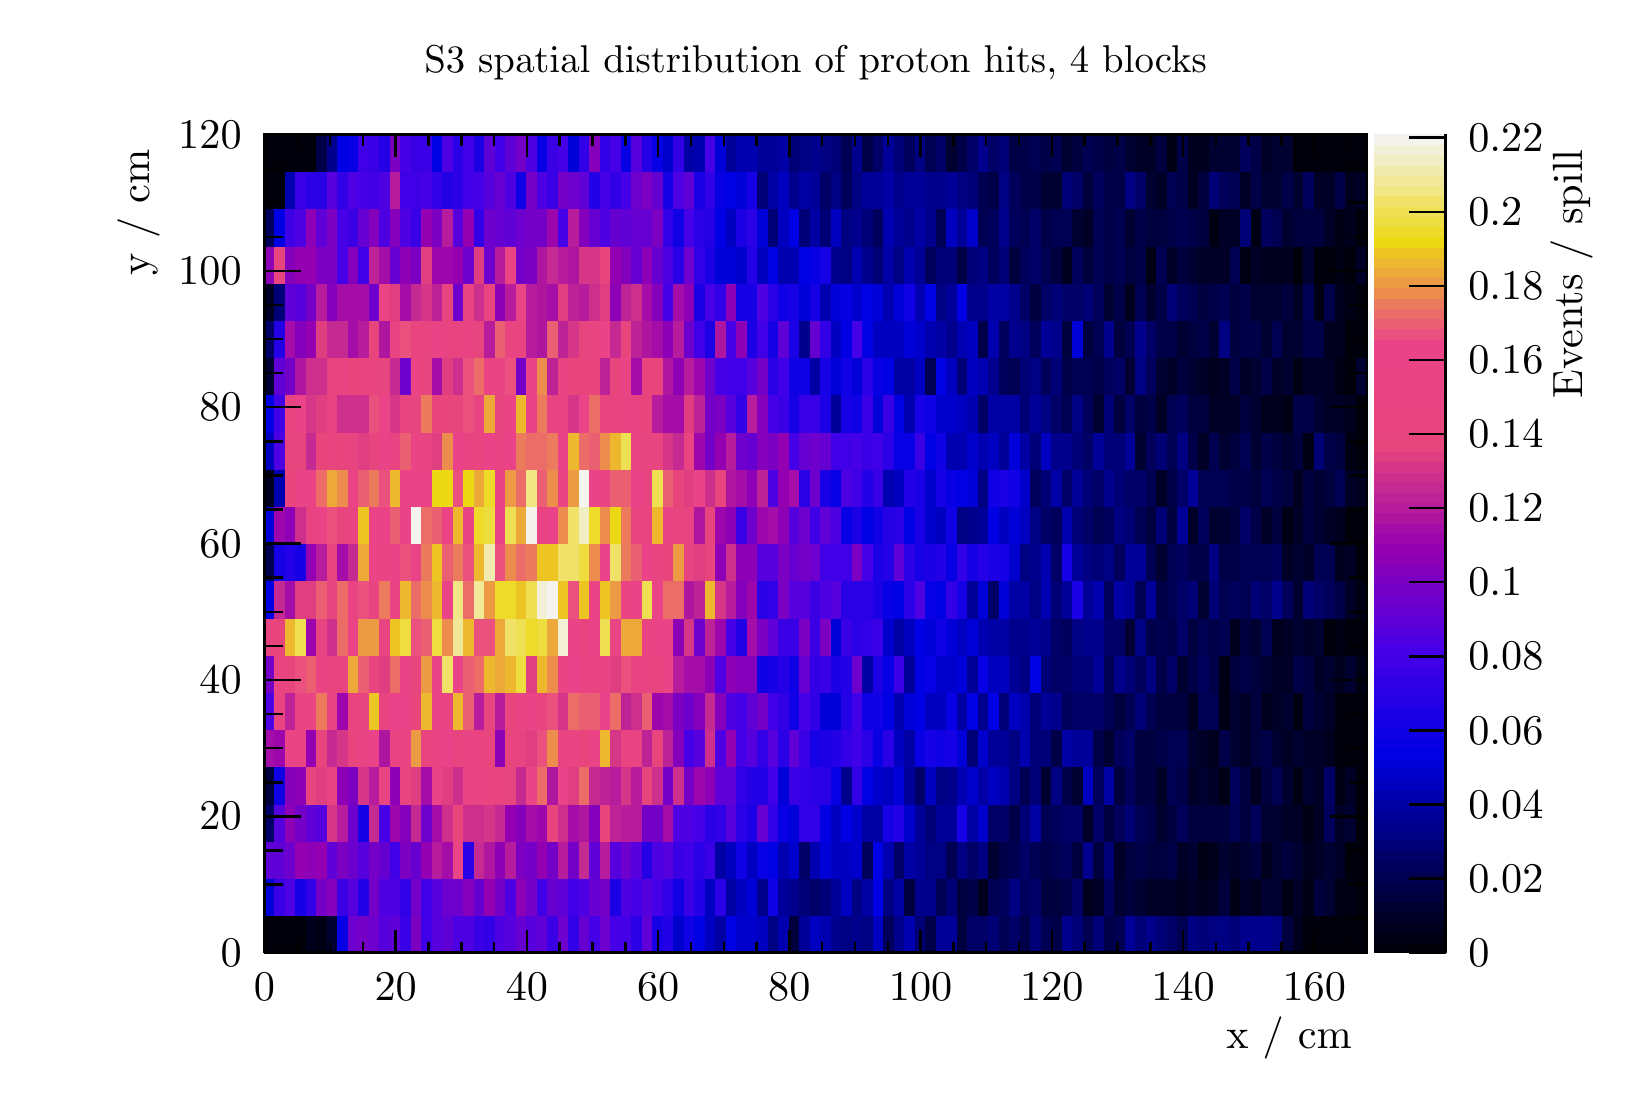
\begin{tikzpicture}
\pgfdeclareplotmark{cross} {
\pgfpathmoveto{\pgfpoint{-0.3\pgfplotmarksize}{\pgfplotmarksize}}
\pgfpathlineto{\pgfpoint{+0.3\pgfplotmarksize}{\pgfplotmarksize}}
\pgfpathlineto{\pgfpoint{+0.3\pgfplotmarksize}{0.3\pgfplotmarksize}}
\pgfpathlineto{\pgfpoint{+1\pgfplotmarksize}{0.3\pgfplotmarksize}}
\pgfpathlineto{\pgfpoint{+1\pgfplotmarksize}{-0.3\pgfplotmarksize}}
\pgfpathlineto{\pgfpoint{+0.3\pgfplotmarksize}{-0.3\pgfplotmarksize}}
\pgfpathlineto{\pgfpoint{+0.3\pgfplotmarksize}{-1.\pgfplotmarksize}}
\pgfpathlineto{\pgfpoint{-0.3\pgfplotmarksize}{-1.\pgfplotmarksize}}
\pgfpathlineto{\pgfpoint{-0.3\pgfplotmarksize}{-0.3\pgfplotmarksize}}
\pgfpathlineto{\pgfpoint{-1.\pgfplotmarksize}{-0.3\pgfplotmarksize}}
\pgfpathlineto{\pgfpoint{-1.\pgfplotmarksize}{0.3\pgfplotmarksize}}
\pgfpathlineto{\pgfpoint{-0.3\pgfplotmarksize}{0.3\pgfplotmarksize}}
\pgfpathclose
\pgfusepathqstroke
}
\pgfdeclareplotmark{cross*} {
\pgfpathmoveto{\pgfpoint{-0.3\pgfplotmarksize}{\pgfplotmarksize}}
\pgfpathlineto{\pgfpoint{+0.3\pgfplotmarksize}{\pgfplotmarksize}}
\pgfpathlineto{\pgfpoint{+0.3\pgfplotmarksize}{0.3\pgfplotmarksize}}
\pgfpathlineto{\pgfpoint{+1\pgfplotmarksize}{0.3\pgfplotmarksize}}
\pgfpathlineto{\pgfpoint{+1\pgfplotmarksize}{-0.3\pgfplotmarksize}}
\pgfpathlineto{\pgfpoint{+0.3\pgfplotmarksize}{-0.3\pgfplotmarksize}}
\pgfpathlineto{\pgfpoint{+0.3\pgfplotmarksize}{-1.\pgfplotmarksize}}
\pgfpathlineto{\pgfpoint{-0.3\pgfplotmarksize}{-1.\pgfplotmarksize}}
\pgfpathlineto{\pgfpoint{-0.3\pgfplotmarksize}{-0.3\pgfplotmarksize}}
\pgfpathlineto{\pgfpoint{-1.\pgfplotmarksize}{-0.3\pgfplotmarksize}}
\pgfpathlineto{\pgfpoint{-1.\pgfplotmarksize}{0.3\pgfplotmarksize}}
\pgfpathlineto{\pgfpoint{-0.3\pgfplotmarksize}{0.3\pgfplotmarksize}}
\pgfpathclose
\pgfusepathqfillstroke
}
\pgfdeclareplotmark{newstar} {
\pgfpathmoveto{\pgfqpoint{0pt}{\pgfplotmarksize}}
\pgfpathlineto{\pgfqpointpolar{44}{0.5\pgfplotmarksize}}
\pgfpathlineto{\pgfqpointpolar{18}{\pgfplotmarksize}}
\pgfpathlineto{\pgfqpointpolar{-20}{0.5\pgfplotmarksize}}
\pgfpathlineto{\pgfqpointpolar{-54}{\pgfplotmarksize}}
\pgfpathlineto{\pgfqpointpolar{-90}{0.5\pgfplotmarksize}}
\pgfpathlineto{\pgfqpointpolar{234}{\pgfplotmarksize}}
\pgfpathlineto{\pgfqpointpolar{198}{0.5\pgfplotmarksize}}
\pgfpathlineto{\pgfqpointpolar{162}{\pgfplotmarksize}}
\pgfpathlineto{\pgfqpointpolar{134}{0.5\pgfplotmarksize}}
\pgfpathclose
\pgfusepathqstroke
}
\pgfdeclareplotmark{newstar*} {
\pgfpathmoveto{\pgfqpoint{0pt}{\pgfplotmarksize}}
\pgfpathlineto{\pgfqpointpolar{44}{0.5\pgfplotmarksize}}
\pgfpathlineto{\pgfqpointpolar{18}{\pgfplotmarksize}}
\pgfpathlineto{\pgfqpointpolar{-20}{0.5\pgfplotmarksize}}
\pgfpathlineto{\pgfqpointpolar{-54}{\pgfplotmarksize}}
\pgfpathlineto{\pgfqpointpolar{-90}{0.5\pgfplotmarksize}}
\pgfpathlineto{\pgfqpointpolar{234}{\pgfplotmarksize}}
\pgfpathlineto{\pgfqpointpolar{198}{0.5\pgfplotmarksize}}
\pgfpathlineto{\pgfqpointpolar{162}{\pgfplotmarksize}}
\pgfpathlineto{\pgfqpointpolar{134}{0.5\pgfplotmarksize}}
\pgfpathclose
\pgfusepathqfillstroke
}
\definecolor{c}{rgb}{1,1,1};
\draw [color=c, fill=c] (0,0) rectangle (20,13.4957);
\draw [color=c, fill=c] (3,1.75444) rectangle (17,12.1461);
\definecolor{c}{rgb}{0,0,0};
\draw [c,line width=0.9] (3,1.75444) -- (3,12.1461) -- (17,12.1461) -- (17,1.75444) -- (3,1.75444);
\definecolor{c}{rgb}{1,1,1};
\draw [color=c, fill=c] (3,1.75444) rectangle (17,12.1461);
\definecolor{c}{rgb}{0,0,0};
\draw [c,line width=0.9] (3,1.75444) -- (3,12.1461) -- (17,12.1461) -- (17,1.75444) -- (3,1.75444);
\definecolor{c}{rgb}{0,0,0.0387097};
\draw [color=c, fill=c] (3,1.75444) rectangle (3.13333,2.22679);
\draw [color=c, fill=c] (3.13333,1.75444) rectangle (3.26667,2.22679);
\draw [color=c, fill=c] (3.26667,1.75444) rectangle (3.4,2.22679);
\draw [color=c, fill=c] (3.4,1.75444) rectangle (3.53333,2.22679);
\definecolor{c}{rgb}{0,0,0.116129};
\draw [color=c, fill=c] (3.53333,1.75444) rectangle (3.66667,2.22679);
\definecolor{c}{rgb}{0,0,0.0774194};
\draw [color=c, fill=c] (3.66667,1.75444) rectangle (3.8,2.22679);
\definecolor{c}{rgb}{0,0,0.193548};
\draw [color=c, fill=c] (3.8,1.75444) rectangle (3.93333,2.22679);
\definecolor{c}{rgb}{0.0257353,0,0.895221};
\draw [color=c, fill=c] (3.93333,1.75444) rectangle (4.06667,2.22679);
\definecolor{c}{rgb}{0.427451,0,0.8};
\draw [color=c, fill=c] (4.06667,1.75444) rectangle (4.2,2.22679);
\definecolor{c}{rgb}{0.456127,0,0.780147};
\draw [color=c, fill=c] (4.2,1.75444) rectangle (4.33333,2.22679);
\definecolor{c}{rgb}{0.427451,0,0.8};
\draw [color=c, fill=c] (4.33333,1.75444) rectangle (4.46667,2.22679);
\definecolor{c}{rgb}{0.331863,0,0.866176};
\draw [color=c, fill=c] (4.46667,1.75444) rectangle (4.6,2.22679);
\definecolor{c}{rgb}{0.370098,0,0.839706};
\draw [color=c, fill=c] (4.6,1.75444) rectangle (4.73333,2.22679);
\definecolor{c}{rgb}{0.223039,0,0.903676};
\draw [color=c, fill=c] (4.73333,1.75444) rectangle (4.86667,2.22679);
\definecolor{c}{rgb}{0.484804,0,0.760294};
\draw [color=c, fill=c] (4.86667,1.75444) rectangle (5,2.22679);
\definecolor{c}{rgb}{0.248775,0,0.904779};
\draw [color=c, fill=c] (5,1.75444) rectangle (5.13333,2.22679);
\definecolor{c}{rgb}{0.331863,0,0.866176};
\draw [color=c, fill=c] (5.13333,1.75444) rectangle (5.26667,2.22679);
\definecolor{c}{rgb}{0.370098,0,0.839706};
\draw [color=c, fill=c] (5.26667,1.75444) rectangle (5.4,2.22679);
\definecolor{c}{rgb}{0.303186,0,0.886029};
\draw [color=c, fill=c] (5.4,1.75444) rectangle (5.53333,2.22679);
\draw [color=c, fill=c] (5.53333,1.75444) rectangle (5.66667,2.22679);
\definecolor{c}{rgb}{0.223039,0,0.903676};
\draw [color=c, fill=c] (5.66667,1.75444) rectangle (5.8,2.22679);
\definecolor{c}{rgb}{0.197304,0,0.902574};
\draw [color=c, fill=c] (5.8,1.75444) rectangle (5.93333,2.22679);
\definecolor{c}{rgb}{0.303186,0,0.886029};
\draw [color=c, fill=c] (5.93333,1.75444) rectangle (6.06667,2.22679);
\definecolor{c}{rgb}{0.331863,0,0.866176};
\draw [color=c, fill=c] (6.06667,1.75444) rectangle (6.2,2.22679);
\definecolor{c}{rgb}{0.398775,0,0.819853};
\draw [color=c, fill=c] (6.2,1.75444) rectangle (6.33333,2.22679);
\definecolor{c}{rgb}{0.331863,0,0.866176};
\draw [color=c, fill=c] (6.33333,1.75444) rectangle (6.46667,2.22679);
\definecolor{c}{rgb}{0.370098,0,0.839706};
\draw [color=c, fill=c] (6.46667,1.75444) rectangle (6.6,2.22679);
\definecolor{c}{rgb}{0.223039,0,0.903676};
\draw [color=c, fill=c] (6.6,1.75444) rectangle (6.73333,2.22679);
\definecolor{c}{rgb}{0.427451,0,0.8};
\draw [color=c, fill=c] (6.73333,1.75444) rectangle (6.86667,2.22679);
\definecolor{c}{rgb}{0.197304,0,0.902574};
\draw [color=c, fill=c] (6.86667,1.75444) rectangle (7,2.22679);
\definecolor{c}{rgb}{0.398775,0,0.819853};
\draw [color=c, fill=c] (7,1.75444) rectangle (7.13333,2.22679);
\definecolor{c}{rgb}{0.27451,0,0.905882};
\draw [color=c, fill=c] (7.13333,1.75444) rectangle (7.26667,2.22679);
\definecolor{c}{rgb}{0.427451,0,0.8};
\draw [color=c, fill=c] (7.26667,1.75444) rectangle (7.4,2.22679);
\definecolor{c}{rgb}{0.27451,0,0.905882};
\draw [color=c, fill=c] (7.4,1.75444) rectangle (7.53333,2.22679);
\draw [color=c, fill=c] (7.53333,1.75444) rectangle (7.66667,2.22679);
\definecolor{c}{rgb}{0.16299,0,0.901103};
\draw [color=c, fill=c] (7.66667,1.75444) rectangle (7.8,2.22679);
\definecolor{c}{rgb}{0.370098,0,0.839706};
\draw [color=c, fill=c] (7.8,1.75444) rectangle (7.93333,2.22679);
\definecolor{c}{rgb}{0.0857843,0,0.897794};
\draw [color=c, fill=c] (7.93333,1.75444) rectangle (8.06667,2.22679);
\definecolor{c}{rgb}{0.137255,0,0.9};
\draw [color=c, fill=c] (8.06667,1.75444) rectangle (8.2,2.22679);
\definecolor{c}{rgb}{0,0,0.801471};
\draw [color=c, fill=c] (8.2,1.75444) rectangle (8.33333,2.22679);
\definecolor{c}{rgb}{0.060049,0,0.896691};
\draw [color=c, fill=c] (8.33333,1.75444) rectangle (8.46667,2.22679);
\definecolor{c}{rgb}{0,0,0.894118};
\draw [color=c, fill=c] (8.46667,1.75444) rectangle (8.6,2.22679);
\definecolor{c}{rgb}{0,0,0.755147};
\draw [color=c, fill=c] (8.6,1.75444) rectangle (8.73333,2.22679);
\definecolor{c}{rgb}{0,0,0.647059};
\draw [color=c, fill=c] (8.73333,1.75444) rectangle (8.86667,2.22679);
\definecolor{c}{rgb}{0,0,0.894118};
\draw [color=c, fill=c] (8.86667,1.75444) rectangle (9,2.22679);
\definecolor{c}{rgb}{0,0,0.801471};
\draw [color=c, fill=c] (9,1.75444) rectangle (9.13333,2.22679);
\draw [color=c, fill=c] (9.13333,1.75444) rectangle (9.26667,2.22679);
\definecolor{c}{rgb}{0,0,0.755147};
\draw [color=c, fill=c] (9.26667,1.75444) rectangle (9.4,2.22679);
\definecolor{c}{rgb}{0,0,0.508088};
\draw [color=c, fill=c] (9.4,1.75444) rectangle (9.53333,2.22679);
\definecolor{c}{rgb}{0,0,0.693382};
\draw [color=c, fill=c] (9.53333,1.75444) rectangle (9.66667,2.22679);
\definecolor{c}{rgb}{0,0,0.245161};
\draw [color=c, fill=c] (9.66667,1.75444) rectangle (9.8,2.22679);
\definecolor{c}{rgb}{0,0,0.600735};
\draw [color=c, fill=c] (9.8,1.75444) rectangle (9.93333,2.22679);
\definecolor{c}{rgb}{0,0,0.755147};
\draw [color=c, fill=c] (9.93333,1.75444) rectangle (10.0667,2.22679);
\definecolor{c}{rgb}{0,0,0.693382};
\draw [color=c, fill=c] (10.0667,1.75444) rectangle (10.2,2.22679);
\definecolor{c}{rgb}{0,0,0.554412};
\draw [color=c, fill=c] (10.2,1.75444) rectangle (10.3333,2.22679);
\definecolor{c}{rgb}{0,0,0.508088};
\draw [color=c, fill=c] (10.3333,1.75444) rectangle (10.4667,2.22679);
\definecolor{c}{rgb}{0,0,0.554412};
\draw [color=c, fill=c] (10.4667,1.75444) rectangle (10.6,2.22679);
\definecolor{c}{rgb}{0,0,0.508088};
\draw [color=c, fill=c] (10.6,1.75444) rectangle (10.7333,2.22679);
\definecolor{c}{rgb}{0,0,0.755147};
\draw [color=c, fill=c] (10.7333,1.75444) rectangle (10.8667,2.22679);
\definecolor{c}{rgb}{0,0,0.36129};
\draw [color=c, fill=c] (10.8667,1.75444) rectangle (11,2.22679);
\definecolor{c}{rgb}{0,0,0.554412};
\draw [color=c, fill=c] (11,1.75444) rectangle (11.1333,2.22679);
\definecolor{c}{rgb}{0,0,0.693382};
\draw [color=c, fill=c] (11.1333,1.75444) rectangle (11.2667,2.22679);
\definecolor{c}{rgb}{0,0,0.461765};
\draw [color=c, fill=c] (11.2667,1.75444) rectangle (11.4,2.22679);
\definecolor{c}{rgb}{0,0,0.283871};
\draw [color=c, fill=c] (11.4,1.75444) rectangle (11.5333,2.22679);
\definecolor{c}{rgb}{0,0,0.600735};
\draw [color=c, fill=c] (11.5333,1.75444) rectangle (11.6667,2.22679);
\draw [color=c, fill=c] (11.6667,1.75444) rectangle (11.8,2.22679);
\definecolor{c}{rgb}{0,0,0.245161};
\draw [color=c, fill=c] (11.8,1.75444) rectangle (11.9333,2.22679);
\definecolor{c}{rgb}{0,0,0.4};
\draw [color=c, fill=c] (11.9333,1.75444) rectangle (12.0667,2.22679);
\draw [color=c, fill=c] (12.0667,1.75444) rectangle (12.2,2.22679);
\definecolor{c}{rgb}{0,0,0.461765};
\draw [color=c, fill=c] (12.2,1.75444) rectangle (12.3333,2.22679);
\definecolor{c}{rgb}{0,0,0.322581};
\draw [color=c, fill=c] (12.3333,1.75444) rectangle (12.4667,2.22679);
\definecolor{c}{rgb}{0,0,0.4};
\draw [color=c, fill=c] (12.4667,1.75444) rectangle (12.6,2.22679);
\definecolor{c}{rgb}{0,0,0.283871};
\draw [color=c, fill=c] (12.6,1.75444) rectangle (12.7333,2.22679);
\definecolor{c}{rgb}{0,0,0.461765};
\draw [color=c, fill=c] (12.7333,1.75444) rectangle (12.8667,2.22679);
\definecolor{c}{rgb}{0,0,0.322581};
\draw [color=c, fill=c] (12.8667,1.75444) rectangle (13,2.22679);
\definecolor{c}{rgb}{0,0,0.283871};
\draw [color=c, fill=c] (13,1.75444) rectangle (13.1333,2.22679);
\definecolor{c}{rgb}{0,0,0.554412};
\draw [color=c, fill=c] (13.1333,1.75444) rectangle (13.2667,2.22679);
\definecolor{c}{rgb}{0,0,0.461765};
\draw [color=c, fill=c] (13.2667,1.75444) rectangle (13.4,2.22679);
\definecolor{c}{rgb}{0,0,0.322581};
\draw [color=c, fill=c] (13.4,1.75444) rectangle (13.5333,2.22679);
\definecolor{c}{rgb}{0,0,0.461765};
\draw [color=c, fill=c] (13.5333,1.75444) rectangle (13.6667,2.22679);
\definecolor{c}{rgb}{0,0,0.283871};
\draw [color=c, fill=c] (13.6667,1.75444) rectangle (13.8,2.22679);
\definecolor{c}{rgb}{0,0,0.322581};
\draw [color=c, fill=c] (13.8,1.75444) rectangle (13.9333,2.22679);
\definecolor{c}{rgb}{0,0,0.600735};
\draw [color=c, fill=c] (13.9333,1.75444) rectangle (14.0667,2.22679);
\definecolor{c}{rgb}{0,0,0.461765};
\draw [color=c, fill=c] (14.0667,1.75444) rectangle (14.2,2.22679);
\definecolor{c}{rgb}{0,0,0.554412};
\draw [color=c, fill=c] (14.2,1.75444) rectangle (14.3333,2.22679);
\definecolor{c}{rgb}{0,0,0.461765};
\draw [color=c, fill=c] (14.3333,1.75444) rectangle (14.4667,2.22679);
\definecolor{c}{rgb}{0,0,0.4};
\draw [color=c, fill=c] (14.4667,1.75444) rectangle (14.6,2.22679);
\definecolor{c}{rgb}{0,0,0.322581};
\draw [color=c, fill=c] (14.6,1.75444) rectangle (14.7333,2.22679);
\definecolor{c}{rgb}{0,0,0.508088};
\draw [color=c, fill=c] (14.7333,1.75444) rectangle (14.8667,2.22679);
\definecolor{c}{rgb}{0,0,0.461765};
\draw [color=c, fill=c] (14.8667,1.75444) rectangle (15,2.22679);
\definecolor{c}{rgb}{0,0,0.508088};
\draw [color=c, fill=c] (15,1.75444) rectangle (15.1333,2.22679);
\draw [color=c, fill=c] (15.1333,1.75444) rectangle (15.2667,2.22679);
\definecolor{c}{rgb}{0,0,0.461765};
\draw [color=c, fill=c] (15.2667,1.75444) rectangle (15.4,2.22679);
\definecolor{c}{rgb}{0,0,0.554412};
\draw [color=c, fill=c] (15.4,1.75444) rectangle (15.5333,2.22679);
\draw [color=c, fill=c] (15.5333,1.75444) rectangle (15.6667,2.22679);
\draw [color=c, fill=c] (15.6667,1.75444) rectangle (15.8,2.22679);
\definecolor{c}{rgb}{0,0,0.508088};
\draw [color=c, fill=c] (15.8,1.75444) rectangle (15.9333,2.22679);
\definecolor{c}{rgb}{0,0,0.245161};
\draw [color=c, fill=c] (15.9333,1.75444) rectangle (16.0667,2.22679);
\definecolor{c}{rgb}{0,0,0.116129};
\draw [color=c, fill=c] (16.0667,1.75444) rectangle (16.2,2.22679);
\definecolor{c}{rgb}{0,0,0.0387097};
\draw [color=c, fill=c] (16.2,1.75444) rectangle (16.3333,2.22679);
\draw [color=c, fill=c] (16.3333,1.75444) rectangle (16.4667,2.22679);
\draw [color=c, fill=c] (16.4667,1.75444) rectangle (16.6,2.22679);
\draw [color=c, fill=c] (16.6,1.75444) rectangle (16.7333,2.22679);
\draw [color=c, fill=c] (16.7333,1.75444) rectangle (16.8667,2.22679);
\draw [color=c, fill=c] (16.8667,1.75444) rectangle (17,2.22679);
\definecolor{c}{rgb}{0,0,0.847794};
\draw [color=c, fill=c] (3,2.22679) rectangle (3.13333,2.69914);
\definecolor{c}{rgb}{0.223039,0,0.903676};
\draw [color=c, fill=c] (3.13333,2.22679) rectangle (3.26667,2.69914);
\definecolor{c}{rgb}{0.303186,0,0.886029};
\draw [color=c, fill=c] (3.26667,2.22679) rectangle (3.4,2.69914);
\definecolor{c}{rgb}{0.0857843,0,0.897794};
\draw [color=c, fill=c] (3.4,2.22679) rectangle (3.53333,2.69914);
\definecolor{c}{rgb}{0.197304,0,0.902574};
\draw [color=c, fill=c] (3.53333,2.22679) rectangle (3.66667,2.69914);
\definecolor{c}{rgb}{0.456127,0,0.780147};
\draw [color=c, fill=c] (3.66667,2.22679) rectangle (3.8,2.69914);
\definecolor{c}{rgb}{0.523039,0,0.733824};
\draw [color=c, fill=c] (3.8,2.22679) rectangle (3.93333,2.69914);
\definecolor{c}{rgb}{0.223039,0,0.903676};
\draw [color=c, fill=c] (3.93333,2.22679) rectangle (4.06667,2.69914);
\definecolor{c}{rgb}{0.331863,0,0.866176};
\draw [color=c, fill=c] (4.06667,2.22679) rectangle (4.2,2.69914);
\definecolor{c}{rgb}{0.137255,0,0.9};
\draw [color=c, fill=c] (4.2,2.22679) rectangle (4.33333,2.69914);
\definecolor{c}{rgb}{0.456127,0,0.780147};
\draw [color=c, fill=c] (4.33333,2.22679) rectangle (4.46667,2.69914);
\definecolor{c}{rgb}{0.303186,0,0.886029};
\draw [color=c, fill=c] (4.46667,2.22679) rectangle (4.6,2.69914);
\draw [color=c, fill=c] (4.6,2.22679) rectangle (4.73333,2.69914);
\definecolor{c}{rgb}{0.197304,0,0.902574};
\draw [color=c, fill=c] (4.73333,2.22679) rectangle (4.86667,2.69914);
\definecolor{c}{rgb}{0.456127,0,0.780147};
\draw [color=c, fill=c] (4.86667,2.22679) rectangle (5,2.69914);
\definecolor{c}{rgb}{0.248775,0,0.904779};
\draw [color=c, fill=c] (5,2.22679) rectangle (5.13333,2.69914);
\definecolor{c}{rgb}{0.331863,0,0.866176};
\draw [color=c, fill=c] (5.13333,2.22679) rectangle (5.26667,2.69914);
\definecolor{c}{rgb}{0.427451,0,0.8};
\draw [color=c, fill=c] (5.26667,2.22679) rectangle (5.4,2.69914);
\draw [color=c, fill=c] (5.4,2.22679) rectangle (5.53333,2.69914);
\definecolor{c}{rgb}{0.523039,0,0.733824};
\draw [color=c, fill=c] (5.53333,2.22679) rectangle (5.66667,2.69914);
\definecolor{c}{rgb}{0.398775,0,0.819853};
\draw [color=c, fill=c] (5.66667,2.22679) rectangle (5.8,2.69914);
\definecolor{c}{rgb}{0.580392,0,0.694118};
\draw [color=c, fill=c] (5.8,2.22679) rectangle (5.93333,2.69914);
\definecolor{c}{rgb}{0.456127,0,0.780147};
\draw [color=c, fill=c] (5.93333,2.22679) rectangle (6.06667,2.69914);
\definecolor{c}{rgb}{0.303186,0,0.886029};
\draw [color=c, fill=c] (6.06667,2.22679) rectangle (6.2,2.69914);
\definecolor{c}{rgb}{0.551716,0,0.713971};
\draw [color=c, fill=c] (6.2,2.22679) rectangle (6.33333,2.69914);
\definecolor{c}{rgb}{0.456127,0,0.780147};
\draw [color=c, fill=c] (6.33333,2.22679) rectangle (6.46667,2.69914);
\definecolor{c}{rgb}{0.248775,0,0.904779};
\draw [color=c, fill=c] (6.46667,2.22679) rectangle (6.6,2.69914);
\definecolor{c}{rgb}{0.398775,0,0.819853};
\draw [color=c, fill=c] (6.6,2.22679) rectangle (6.73333,2.69914);
\definecolor{c}{rgb}{0.370098,0,0.839706};
\draw [color=c, fill=c] (6.73333,2.22679) rectangle (6.86667,2.69914);
\definecolor{c}{rgb}{0.248775,0,0.904779};
\draw [color=c, fill=c] (6.86667,2.22679) rectangle (7,2.69914);
\definecolor{c}{rgb}{0.303186,0,0.886029};
\draw [color=c, fill=c] (7,2.22679) rectangle (7.13333,2.69914);
\definecolor{c}{rgb}{0.398775,0,0.819853};
\draw [color=c, fill=c] (7.13333,2.22679) rectangle (7.26667,2.69914);
\definecolor{c}{rgb}{0.456127,0,0.780147};
\draw [color=c, fill=c] (7.26667,2.22679) rectangle (7.4,2.69914);
\definecolor{c}{rgb}{0.11152,0,0.898897};
\draw [color=c, fill=c] (7.4,2.22679) rectangle (7.53333,2.69914);
\definecolor{c}{rgb}{0.303186,0,0.886029};
\draw [color=c, fill=c] (7.53333,2.22679) rectangle (7.66667,2.69914);
\definecolor{c}{rgb}{0.27451,0,0.905882};
\draw [color=c, fill=c] (7.66667,2.22679) rectangle (7.8,2.69914);
\definecolor{c}{rgb}{0.331863,0,0.866176};
\draw [color=c, fill=c] (7.8,2.22679) rectangle (7.93333,2.69914);
\definecolor{c}{rgb}{0.27451,0,0.905882};
\draw [color=c, fill=c] (7.93333,2.22679) rectangle (8.06667,2.69914);
\definecolor{c}{rgb}{0.197304,0,0.902574};
\draw [color=c, fill=c] (8.06667,2.22679) rectangle (8.2,2.69914);
\definecolor{c}{rgb}{0.060049,0,0.896691};
\draw [color=c, fill=c] (8.2,2.22679) rectangle (8.33333,2.69914);
\definecolor{c}{rgb}{0.223039,0,0.903676};
\draw [color=c, fill=c] (8.33333,2.22679) rectangle (8.46667,2.69914);
\definecolor{c}{rgb}{0.137255,0,0.9};
\draw [color=c, fill=c] (8.46667,2.22679) rectangle (8.6,2.69914);
\definecolor{c}{rgb}{0,0,0.755147};
\draw [color=c, fill=c] (8.6,2.22679) rectangle (8.73333,2.69914);
\definecolor{c}{rgb}{0.16299,0,0.901103};
\draw [color=c, fill=c] (8.73333,2.22679) rectangle (8.86667,2.69914);
\definecolor{c}{rgb}{0,0,0.647059};
\draw [color=c, fill=c] (8.86667,2.22679) rectangle (9,2.69914);
\definecolor{c}{rgb}{0,0,0.755147};
\draw [color=c, fill=c] (9,2.22679) rectangle (9.13333,2.69914);
\definecolor{c}{rgb}{0,0,0.847794};
\draw [color=c, fill=c] (9.13333,2.22679) rectangle (9.26667,2.69914);
\definecolor{c}{rgb}{0,0,0.554412};
\draw [color=c, fill=c] (9.26667,2.22679) rectangle (9.4,2.69914);
\definecolor{c}{rgb}{0.060049,0,0.896691};
\draw [color=c, fill=c] (9.4,2.22679) rectangle (9.53333,2.69914);
\definecolor{c}{rgb}{0,0,0.600735};
\draw [color=c, fill=c] (9.53333,2.22679) rectangle (9.66667,2.69914);
\definecolor{c}{rgb}{0,0,0.554412};
\draw [color=c, fill=c] (9.66667,2.22679) rectangle (9.8,2.69914);
\definecolor{c}{rgb}{0,0,0.461765};
\draw [color=c, fill=c] (9.8,2.22679) rectangle (9.93333,2.69914);
\definecolor{c}{rgb}{0,0,0.4};
\draw [color=c, fill=c] (9.93333,2.22679) rectangle (10.0667,2.69914);
\definecolor{c}{rgb}{0,0,0.461765};
\draw [color=c, fill=c] (10.0667,2.22679) rectangle (10.2,2.69914);
\definecolor{c}{rgb}{0,0,0.600735};
\draw [color=c, fill=c] (10.2,2.22679) rectangle (10.3333,2.69914);
\definecolor{c}{rgb}{0,0,0.755147};
\draw [color=c, fill=c] (10.3333,2.22679) rectangle (10.4667,2.69914);
\definecolor{c}{rgb}{0,0,0.508088};
\draw [color=c, fill=c] (10.4667,2.22679) rectangle (10.6,2.69914);
\definecolor{c}{rgb}{0,0,0.647059};
\draw [color=c, fill=c] (10.6,2.22679) rectangle (10.7333,2.69914);
\definecolor{c}{rgb}{0,0,0.894118};
\draw [color=c, fill=c] (10.7333,2.22679) rectangle (10.8667,2.69914);
\definecolor{c}{rgb}{0,0,0.508088};
\draw [color=c, fill=c] (10.8667,2.22679) rectangle (11,2.69914);
\definecolor{c}{rgb}{0,0,0.647059};
\draw [color=c, fill=c] (11,2.22679) rectangle (11.1333,2.69914);
\definecolor{c}{rgb}{0,0,0.245161};
\draw [color=c, fill=c] (11.1333,2.22679) rectangle (11.2667,2.69914);
\definecolor{c}{rgb}{0,0,0.554412};
\draw [color=c, fill=c] (11.2667,2.22679) rectangle (11.4,2.69914);
\draw [color=c, fill=c] (11.4,2.22679) rectangle (11.5333,2.69914);
\definecolor{c}{rgb}{0,0,0.322581};
\draw [color=c, fill=c] (11.5333,2.22679) rectangle (11.6667,2.69914);
\definecolor{c}{rgb}{0,0,0.461765};
\draw [color=c, fill=c] (11.6667,2.22679) rectangle (11.8,2.69914);
\definecolor{c}{rgb}{0,0,0.245161};
\draw [color=c, fill=c] (11.8,2.22679) rectangle (11.9333,2.69914);
\definecolor{c}{rgb}{0,0,0.283871};
\draw [color=c, fill=c] (11.9333,2.22679) rectangle (12.0667,2.69914);
\definecolor{c}{rgb}{0,0,0.116129};
\draw [color=c, fill=c] (12.0667,2.22679) rectangle (12.2,2.69914);
\definecolor{c}{rgb}{0,0,0.322581};
\draw [color=c, fill=c] (12.2,2.22679) rectangle (12.3333,2.69914);
\definecolor{c}{rgb}{0,0,0.36129};
\draw [color=c, fill=c] (12.3333,2.22679) rectangle (12.4667,2.69914);
\definecolor{c}{rgb}{0,0,0.508088};
\draw [color=c, fill=c] (12.4667,2.22679) rectangle (12.6,2.69914);
\definecolor{c}{rgb}{0,0,0.36129};
\draw [color=c, fill=c] (12.6,2.22679) rectangle (12.7333,2.69914);
\definecolor{c}{rgb}{0,0,0.4};
\draw [color=c, fill=c] (12.7333,2.22679) rectangle (12.8667,2.69914);
\definecolor{c}{rgb}{0,0,0.245161};
\draw [color=c, fill=c] (12.8667,2.22679) rectangle (13,2.69914);
\draw [color=c, fill=c] (13,2.22679) rectangle (13.1333,2.69914);
\definecolor{c}{rgb}{0,0,0.283871};
\draw [color=c, fill=c] (13.1333,2.22679) rectangle (13.2667,2.69914);
\definecolor{c}{rgb}{0,0,0.4};
\draw [color=c, fill=c] (13.2667,2.22679) rectangle (13.4,2.69914);
\definecolor{c}{rgb}{0,0,0.116129};
\draw [color=c, fill=c] (13.4,2.22679) rectangle (13.5333,2.69914);
\definecolor{c}{rgb}{0,0,0.154839};
\draw [color=c, fill=c] (13.5333,2.22679) rectangle (13.6667,2.69914);
\definecolor{c}{rgb}{0,0,0.36129};
\draw [color=c, fill=c] (13.6667,2.22679) rectangle (13.8,2.69914);
\definecolor{c}{rgb}{0,0,0.193548};
\draw [color=c, fill=c] (13.8,2.22679) rectangle (13.9333,2.69914);
\definecolor{c}{rgb}{0,0,0.245161};
\draw [color=c, fill=c] (13.9333,2.22679) rectangle (14.0667,2.69914);
\definecolor{c}{rgb}{0,0,0.193548};
\draw [color=c, fill=c] (14.0667,2.22679) rectangle (14.2,2.69914);
\definecolor{c}{rgb}{0,0,0.154839};
\draw [color=c, fill=c] (14.2,2.22679) rectangle (14.3333,2.69914);
\draw [color=c, fill=c] (14.3333,2.22679) rectangle (14.4667,2.69914);
\draw [color=c, fill=c] (14.4667,2.22679) rectangle (14.6,2.69914);
\definecolor{c}{rgb}{0,0,0.116129};
\draw [color=c, fill=c] (14.6,2.22679) rectangle (14.7333,2.69914);
\definecolor{c}{rgb}{0,0,0.154839};
\draw [color=c, fill=c] (14.7333,2.22679) rectangle (14.8667,2.69914);
\definecolor{c}{rgb}{0,0,0.116129};
\draw [color=c, fill=c] (14.8667,2.22679) rectangle (15,2.69914);
\definecolor{c}{rgb}{0,0,0.154839};
\draw [color=c, fill=c] (15,2.22679) rectangle (15.1333,2.69914);
\definecolor{c}{rgb}{0,0,0.245161};
\draw [color=c, fill=c] (15.1333,2.22679) rectangle (15.2667,2.69914);
\definecolor{c}{rgb}{0,0,0.0774194};
\draw [color=c, fill=c] (15.2667,2.22679) rectangle (15.4,2.69914);
\definecolor{c}{rgb}{0,0,0.154839};
\draw [color=c, fill=c] (15.4,2.22679) rectangle (15.5333,2.69914);
\definecolor{c}{rgb}{0,0,0.116129};
\draw [color=c, fill=c] (15.5333,2.22679) rectangle (15.6667,2.69914);
\definecolor{c}{rgb}{0,0,0.193548};
\draw [color=c, fill=c] (15.6667,2.22679) rectangle (15.8,2.69914);
\draw [color=c, fill=c] (15.8,2.22679) rectangle (15.9333,2.69914);
\definecolor{c}{rgb}{0,0,0.0774194};
\draw [color=c, fill=c] (15.9333,2.22679) rectangle (16.0667,2.69914);
\definecolor{c}{rgb}{0,0,0.154839};
\draw [color=c, fill=c] (16.0667,2.22679) rectangle (16.2,2.69914);
\definecolor{c}{rgb}{0,0,0.0774194};
\draw [color=c, fill=c] (16.2,2.22679) rectangle (16.3333,2.69914);
\definecolor{c}{rgb}{0,0,0.245161};
\draw [color=c, fill=c] (16.3333,2.22679) rectangle (16.4667,2.69914);
\definecolor{c}{rgb}{0,0,0.193548};
\draw [color=c, fill=c] (16.4667,2.22679) rectangle (16.6,2.69914);
\definecolor{c}{rgb}{0,0,0.0774194};
\draw [color=c, fill=c] (16.6,2.22679) rectangle (16.7333,2.69914);
\draw [color=c, fill=c] (16.7333,2.22679) rectangle (16.8667,2.69914);
\definecolor{c}{rgb}{0,0,0.0387097};
\draw [color=c, fill=c] (16.8667,2.22679) rectangle (17,2.69914);
\definecolor{c}{rgb}{0.370098,0,0.839706};
\draw [color=c, fill=c] (3,2.69914) rectangle (3.13333,3.17149);
\draw [color=c, fill=c] (3.13333,2.69914) rectangle (3.26667,3.17149);
\definecolor{c}{rgb}{0.427451,0,0.8};
\draw [color=c, fill=c] (3.26667,2.69914) rectangle (3.4,3.17149);
\definecolor{c}{rgb}{0.580392,0,0.694118};
\draw [color=c, fill=c] (3.4,2.69914) rectangle (3.53333,3.17149);
\definecolor{c}{rgb}{0.551716,0,0.713971};
\draw [color=c, fill=c] (3.53333,2.69914) rectangle (3.66667,3.17149);
\definecolor{c}{rgb}{0.580392,0,0.694118};
\draw [color=c, fill=c] (3.66667,2.69914) rectangle (3.8,3.17149);
\definecolor{c}{rgb}{0.370098,0,0.839706};
\draw [color=c, fill=c] (3.8,2.69914) rectangle (3.93333,3.17149);
\definecolor{c}{rgb}{0.484804,0,0.760294};
\draw [color=c, fill=c] (3.93333,2.69914) rectangle (4.06667,3.17149);
\definecolor{c}{rgb}{0.427451,0,0.8};
\draw [color=c, fill=c] (4.06667,2.69914) rectangle (4.2,3.17149);
\definecolor{c}{rgb}{0.331863,0,0.866176};
\draw [color=c, fill=c] (4.2,2.69914) rectangle (4.33333,3.17149);
\definecolor{c}{rgb}{0.456127,0,0.780147};
\draw [color=c, fill=c] (4.33333,2.69914) rectangle (4.46667,3.17149);
\definecolor{c}{rgb}{0.398775,0,0.819853};
\draw [color=c, fill=c] (4.46667,2.69914) rectangle (4.6,3.17149);
\definecolor{c}{rgb}{0.248775,0,0.904779};
\draw [color=c, fill=c] (4.6,2.69914) rectangle (4.73333,3.17149);
\definecolor{c}{rgb}{0.484804,0,0.760294};
\draw [color=c, fill=c] (4.73333,2.69914) rectangle (4.86667,3.17149);
\definecolor{c}{rgb}{0.398775,0,0.819853};
\draw [color=c, fill=c] (4.86667,2.69914) rectangle (5,3.17149);
\definecolor{c}{rgb}{0.580392,0,0.694118};
\draw [color=c, fill=c] (5,2.69914) rectangle (5.13333,3.17149);
\definecolor{c}{rgb}{0.712623,0.109926,0.609681};
\draw [color=c, fill=c] (5.13333,2.69914) rectangle (5.26667,3.17149);
\definecolor{c}{rgb}{0.641422,0.0507353,0.655147};
\draw [color=c, fill=c] (5.26667,2.69914) rectangle (5.4,3.17149);
\definecolor{c}{rgb}{0.915196,0.265931,0.516544};
\draw [color=c, fill=c] (5.4,2.69914) rectangle (5.53333,3.17149);
\definecolor{c}{rgb}{0.16299,0,0.901103};
\draw [color=c, fill=c] (5.53333,2.69914) rectangle (5.66667,3.17149);
\definecolor{c}{rgb}{0.773652,0.160662,0.570711};
\draw [color=c, fill=c] (5.66667,2.69914) rectangle (5.8,3.17149);
\definecolor{c}{rgb}{0.682108,0.0845588,0.629167};
\draw [color=c, fill=c] (5.8,2.69914) rectangle (5.93333,3.17149);
\definecolor{c}{rgb}{0.551716,0,0.713971};
\draw [color=c, fill=c] (5.93333,2.69914) rectangle (6.06667,3.17149);
\definecolor{c}{rgb}{0.712623,0.109926,0.609681};
\draw [color=c, fill=c] (6.06667,2.69914) rectangle (6.2,3.17149);
\definecolor{c}{rgb}{0.484804,0,0.760294};
\draw [color=c, fill=c] (6.2,2.69914) rectangle (6.33333,3.17149);
\definecolor{c}{rgb}{0.456127,0,0.780147};
\draw [color=c, fill=c] (6.33333,2.69914) rectangle (6.46667,3.17149);
\definecolor{c}{rgb}{0.580392,0,0.694118};
\draw [color=c, fill=c] (6.46667,2.69914) rectangle (6.6,3.17149);
\definecolor{c}{rgb}{0.456127,0,0.780147};
\draw [color=c, fill=c] (6.6,2.69914) rectangle (6.73333,3.17149);
\definecolor{c}{rgb}{0.712623,0.109926,0.609681};
\draw [color=c, fill=c] (6.73333,2.69914) rectangle (6.86667,3.17149);
\definecolor{c}{rgb}{0.456127,0,0.780147};
\draw [color=c, fill=c] (6.86667,2.69914) rectangle (7,3.17149);
\definecolor{c}{rgb}{0.773652,0.160662,0.570711};
\draw [color=c, fill=c] (7,2.69914) rectangle (7.13333,3.17149);
\definecolor{c}{rgb}{0.370098,0,0.839706};
\draw [color=c, fill=c] (7.13333,2.69914) rectangle (7.26667,3.17149);
\definecolor{c}{rgb}{0.712623,0.109926,0.609681};
\draw [color=c, fill=c] (7.26667,2.69914) rectangle (7.4,3.17149);
\definecolor{c}{rgb}{0.331863,0,0.866176};
\draw [color=c, fill=c] (7.4,2.69914) rectangle (7.53333,3.17149);
\definecolor{c}{rgb}{0.427451,0,0.8};
\draw [color=c, fill=c] (7.53333,2.69914) rectangle (7.66667,3.17149);
\definecolor{c}{rgb}{0.331863,0,0.866176};
\draw [color=c, fill=c] (7.66667,2.69914) rectangle (7.8,3.17149);
\definecolor{c}{rgb}{0.137255,0,0.9};
\draw [color=c, fill=c] (7.8,2.69914) rectangle (7.93333,3.17149);
\definecolor{c}{rgb}{0.303186,0,0.886029};
\draw [color=c, fill=c] (7.93333,2.69914) rectangle (8.06667,3.17149);
\definecolor{c}{rgb}{0.331863,0,0.866176};
\draw [color=c, fill=c] (8.06667,2.69914) rectangle (8.2,3.17149);
\definecolor{c}{rgb}{0.223039,0,0.903676};
\draw [color=c, fill=c] (8.2,2.69914) rectangle (8.33333,3.17149);
\definecolor{c}{rgb}{0.248775,0,0.904779};
\draw [color=c, fill=c] (8.33333,2.69914) rectangle (8.46667,3.17149);
\definecolor{c}{rgb}{0.16299,0,0.901103};
\draw [color=c, fill=c] (8.46667,2.69914) rectangle (8.6,3.17149);
\definecolor{c}{rgb}{0.223039,0,0.903676};
\draw [color=c, fill=c] (8.6,2.69914) rectangle (8.73333,3.17149);
\definecolor{c}{rgb}{0,0,0.647059};
\draw [color=c, fill=c] (8.73333,2.69914) rectangle (8.86667,3.17149);
\definecolor{c}{rgb}{0,0,0.755147};
\draw [color=c, fill=c] (8.86667,2.69914) rectangle (9,3.17149);
\definecolor{c}{rgb}{0.060049,0,0.896691};
\draw [color=c, fill=c] (9,2.69914) rectangle (9.13333,3.17149);
\definecolor{c}{rgb}{0,0,0.755147};
\draw [color=c, fill=c] (9.13333,2.69914) rectangle (9.26667,3.17149);
\definecolor{c}{rgb}{0.0257353,0,0.895221};
\draw [color=c, fill=c] (9.26667,2.69914) rectangle (9.4,3.17149);
\definecolor{c}{rgb}{0,0,0.894118};
\draw [color=c, fill=c] (9.4,2.69914) rectangle (9.53333,3.17149);
\definecolor{c}{rgb}{0,0,0.693382};
\draw [color=c, fill=c] (9.53333,2.69914) rectangle (9.66667,3.17149);
\definecolor{c}{rgb}{0,0,0.801471};
\draw [color=c, fill=c] (9.66667,2.69914) rectangle (9.8,3.17149);
\definecolor{c}{rgb}{0,0,0.4};
\draw [color=c, fill=c] (9.8,2.69914) rectangle (9.93333,3.17149);
\definecolor{c}{rgb}{0,0,0.693382};
\draw [color=c, fill=c] (9.93333,2.69914) rectangle (10.0667,3.17149);
\definecolor{c}{rgb}{0,0,0.847794};
\draw [color=c, fill=c] (10.0667,2.69914) rectangle (10.2,3.17149);
\definecolor{c}{rgb}{0,0,0.755147};
\draw [color=c, fill=c] (10.2,2.69914) rectangle (10.3333,3.17149);
\draw [color=c, fill=c] (10.3333,2.69914) rectangle (10.4667,3.17149);
\definecolor{c}{rgb}{0,0,0.801471};
\draw [color=c, fill=c] (10.4667,2.69914) rectangle (10.6,3.17149);
\definecolor{c}{rgb}{0,0,0.36129};
\draw [color=c, fill=c] (10.6,2.69914) rectangle (10.7333,3.17149);
\definecolor{c}{rgb}{0,0,0.894118};
\draw [color=c, fill=c] (10.7333,2.69914) rectangle (10.8667,3.17149);
\definecolor{c}{rgb}{0,0,0.693382};
\draw [color=c, fill=c] (10.8667,2.69914) rectangle (11,3.17149);
\definecolor{c}{rgb}{0,0,0.4};
\draw [color=c, fill=c] (11,2.69914) rectangle (11.1333,3.17149);
\definecolor{c}{rgb}{0,0,0.647059};
\draw [color=c, fill=c] (11.1333,2.69914) rectangle (11.2667,3.17149);
\definecolor{c}{rgb}{0,0,0.600735};
\draw [color=c, fill=c] (11.2667,2.69914) rectangle (11.4,3.17149);
\definecolor{c}{rgb}{0,0,0.508088};
\draw [color=c, fill=c] (11.4,2.69914) rectangle (11.5333,3.17149);
\draw [color=c, fill=c] (11.5333,2.69914) rectangle (11.6667,3.17149);
\definecolor{c}{rgb}{0,0,0.322581};
\draw [color=c, fill=c] (11.6667,2.69914) rectangle (11.8,3.17149);
\definecolor{c}{rgb}{0,0,0.508088};
\draw [color=c, fill=c] (11.8,2.69914) rectangle (11.9333,3.17149);
\definecolor{c}{rgb}{0,0,0.4};
\draw [color=c, fill=c] (11.9333,2.69914) rectangle (12.0667,3.17149);
\definecolor{c}{rgb}{0,0,0.508088};
\draw [color=c, fill=c] (12.0667,2.69914) rectangle (12.2,3.17149);
\definecolor{c}{rgb}{0,0,0.193548};
\draw [color=c, fill=c] (12.2,2.69914) rectangle (12.3333,3.17149);
\definecolor{c}{rgb}{0,0,0.283871};
\draw [color=c, fill=c] (12.3333,2.69914) rectangle (12.4667,3.17149);
\definecolor{c}{rgb}{0,0,0.322581};
\draw [color=c, fill=c] (12.4667,2.69914) rectangle (12.6,3.17149);
\definecolor{c}{rgb}{0,0,0.4};
\draw [color=c, fill=c] (12.6,2.69914) rectangle (12.7333,3.17149);
\definecolor{c}{rgb}{0,0,0.322581};
\draw [color=c, fill=c] (12.7333,2.69914) rectangle (12.8667,3.17149);
\definecolor{c}{rgb}{0,0,0.283871};
\draw [color=c, fill=c] (12.8667,2.69914) rectangle (13,3.17149);
\definecolor{c}{rgb}{0,0,0.322581};
\draw [color=c, fill=c] (13,2.69914) rectangle (13.1333,3.17149);
\definecolor{c}{rgb}{0,0,0.36129};
\draw [color=c, fill=c] (13.1333,2.69914) rectangle (13.2667,3.17149);
\definecolor{c}{rgb}{0,0,0.245161};
\draw [color=c, fill=c] (13.2667,2.69914) rectangle (13.4,3.17149);
\definecolor{c}{rgb}{0,0,0.554412};
\draw [color=c, fill=c] (13.4,2.69914) rectangle (13.5333,3.17149);
\definecolor{c}{rgb}{0,0,0.245161};
\draw [color=c, fill=c] (13.5333,2.69914) rectangle (13.6667,3.17149);
\definecolor{c}{rgb}{0,0,0.461765};
\draw [color=c, fill=c] (13.6667,2.69914) rectangle (13.8,3.17149);
\definecolor{c}{rgb}{0,0,0.154839};
\draw [color=c, fill=c] (13.8,2.69914) rectangle (13.9333,3.17149);
\definecolor{c}{rgb}{0,0,0.245161};
\draw [color=c, fill=c] (13.9333,2.69914) rectangle (14.0667,3.17149);
\definecolor{c}{rgb}{0,0,0.283871};
\draw [color=c, fill=c] (14.0667,2.69914) rectangle (14.2,3.17149);
\definecolor{c}{rgb}{0,0,0.245161};
\draw [color=c, fill=c] (14.2,2.69914) rectangle (14.3333,3.17149);
\draw [color=c, fill=c] (14.3333,2.69914) rectangle (14.4667,3.17149);
\definecolor{c}{rgb}{0,0,0.283871};
\draw [color=c, fill=c] (14.4667,2.69914) rectangle (14.6,3.17149);
\definecolor{c}{rgb}{0,0,0.154839};
\draw [color=c, fill=c] (14.6,2.69914) rectangle (14.7333,3.17149);
\definecolor{c}{rgb}{0,0,0.193548};
\draw [color=c, fill=c] (14.7333,2.69914) rectangle (14.8667,3.17149);
\definecolor{c}{rgb}{0,0,0.0774194};
\draw [color=c, fill=c] (14.8667,2.69914) rectangle (15,3.17149);
\definecolor{c}{rgb}{0,0,0.116129};
\draw [color=c, fill=c] (15,2.69914) rectangle (15.1333,3.17149);
\definecolor{c}{rgb}{0,0,0.193548};
\draw [color=c, fill=c] (15.1333,2.69914) rectangle (15.2667,3.17149);
\definecolor{c}{rgb}{0,0,0.154839};
\draw [color=c, fill=c] (15.2667,2.69914) rectangle (15.4,3.17149);
\definecolor{c}{rgb}{0,0,0.193548};
\draw [color=c, fill=c] (15.4,2.69914) rectangle (15.5333,3.17149);
\definecolor{c}{rgb}{0,0,0.245161};
\draw [color=c, fill=c] (15.5333,2.69914) rectangle (15.6667,3.17149);
\definecolor{c}{rgb}{0,0,0.116129};
\draw [color=c, fill=c] (15.6667,2.69914) rectangle (15.8,3.17149);
\definecolor{c}{rgb}{0,0,0.193548};
\draw [color=c, fill=c] (15.8,2.69914) rectangle (15.9333,3.17149);
\definecolor{c}{rgb}{0,0,0.245161};
\draw [color=c, fill=c] (15.9333,2.69914) rectangle (16.0667,3.17149);
\definecolor{c}{rgb}{0,0,0.193548};
\draw [color=c, fill=c] (16.0667,2.69914) rectangle (16.2,3.17149);
\definecolor{c}{rgb}{0,0,0.116129};
\draw [color=c, fill=c] (16.2,2.69914) rectangle (16.3333,3.17149);
\definecolor{c}{rgb}{0,0,0.154839};
\draw [color=c, fill=c] (16.3333,2.69914) rectangle (16.4667,3.17149);
\definecolor{c}{rgb}{0,0,0.193548};
\draw [color=c, fill=c] (16.4667,2.69914) rectangle (16.6,3.17149);
\definecolor{c}{rgb}{0,0,0.154839};
\draw [color=c, fill=c] (16.6,2.69914) rectangle (16.7333,3.17149);
\definecolor{c}{rgb}{0,0,0.0387097};
\draw [color=c, fill=c] (16.7333,2.69914) rectangle (16.8667,3.17149);
\draw [color=c, fill=c] (16.8667,2.69914) rectangle (17,3.17149);
\definecolor{c}{rgb}{0,0,0.4};
\draw [color=c, fill=c] (3,3.17149) rectangle (3.13333,3.64384);
\definecolor{c}{rgb}{0.331863,0,0.866176};
\draw [color=c, fill=c] (3.13333,3.17149) rectangle (3.26667,3.64384);
\definecolor{c}{rgb}{0.551716,0,0.713971};
\draw [color=c, fill=c] (3.26667,3.17149) rectangle (3.4,3.64384);
\definecolor{c}{rgb}{0.456127,0,0.780147};
\draw [color=c, fill=c] (3.4,3.17149) rectangle (3.53333,3.64384);
\definecolor{c}{rgb}{0.370098,0,0.839706};
\draw [color=c, fill=c] (3.53333,3.17149) rectangle (3.66667,3.64384);
\definecolor{c}{rgb}{0.331863,0,0.866176};
\draw [color=c, fill=c] (3.66667,3.17149) rectangle (3.8,3.64384);
\definecolor{c}{rgb}{0.834681,0.211397,0.53174};
\draw [color=c, fill=c] (3.8,3.17149) rectangle (3.93333,3.64384);
\definecolor{c}{rgb}{0.712623,0.109926,0.609681};
\draw [color=c, fill=c] (3.93333,3.17149) rectangle (4.06667,3.64384);
\definecolor{c}{rgb}{0.427451,0,0.8};
\draw [color=c, fill=c] (4.06667,3.17149) rectangle (4.2,3.64384);
\definecolor{c}{rgb}{0.0857843,0,0.897794};
\draw [color=c, fill=c] (4.2,3.17149) rectangle (4.33333,3.64384);
\definecolor{c}{rgb}{0.773652,0.160662,0.570711};
\draw [color=c, fill=c] (4.33333,3.17149) rectangle (4.46667,3.64384);
\definecolor{c}{rgb}{0.27451,0,0.905882};
\draw [color=c, fill=c] (4.46667,3.17149) rectangle (4.6,3.64384);
\definecolor{c}{rgb}{0.610907,0.0253676,0.674632};
\draw [color=c, fill=c] (4.6,3.17149) rectangle (4.73333,3.64384);
\definecolor{c}{rgb}{0.523039,0,0.733824};
\draw [color=c, fill=c] (4.73333,3.17149) rectangle (4.86667,3.64384);
\definecolor{c}{rgb}{0.773652,0.160662,0.570711};
\draw [color=c, fill=c] (4.86667,3.17149) rectangle (5,3.64384);
\definecolor{c}{rgb}{0.427451,0,0.8};
\draw [color=c, fill=c] (5,3.17149) rectangle (5.13333,3.64384);
\definecolor{c}{rgb}{0.641422,0.0507353,0.655147};
\draw [color=c, fill=c] (5.13333,3.17149) rectangle (5.26667,3.64384);
\definecolor{c}{rgb}{0.804167,0.186029,0.551225};
\draw [color=c, fill=c] (5.26667,3.17149) rectangle (5.4,3.64384);
\definecolor{c}{rgb}{0.905882,0.270588,0.486275};
\draw [color=c, fill=c] (5.4,3.17149) rectangle (5.53333,3.64384);
\definecolor{c}{rgb}{0.804167,0.186029,0.551225};
\draw [color=c, fill=c] (5.53333,3.17149) rectangle (5.66667,3.64384);
\draw [color=c, fill=c] (5.66667,3.17149) rectangle (5.8,3.64384);
\definecolor{c}{rgb}{0.834681,0.211397,0.53174};
\draw [color=c, fill=c] (5.8,3.17149) rectangle (5.93333,3.64384);
\definecolor{c}{rgb}{0.773652,0.160662,0.570711};
\draw [color=c, fill=c] (5.93333,3.17149) rectangle (6.06667,3.64384);
\definecolor{c}{rgb}{0.580392,0,0.694118};
\draw [color=c, fill=c] (6.06667,3.17149) rectangle (6.2,3.64384);
\definecolor{c}{rgb}{0.523039,0,0.733824};
\draw [color=c, fill=c] (6.2,3.17149) rectangle (6.33333,3.64384);
\definecolor{c}{rgb}{0.641422,0.0507353,0.655147};
\draw [color=c, fill=c] (6.33333,3.17149) rectangle (6.46667,3.64384);
\definecolor{c}{rgb}{0.610907,0.0253676,0.674632};
\draw [color=c, fill=c] (6.46667,3.17149) rectangle (6.6,3.64384);
\definecolor{c}{rgb}{0.905882,0.270588,0.486275};
\draw [color=c, fill=c] (6.6,3.17149) rectangle (6.73333,3.64384);
\definecolor{c}{rgb}{0.804167,0.186029,0.551225};
\draw [color=c, fill=c] (6.73333,3.17149) rectangle (6.86667,3.64384);
\definecolor{c}{rgb}{0.641422,0.0507353,0.655147};
\draw [color=c, fill=c] (6.86667,3.17149) rectangle (7,3.64384);
\definecolor{c}{rgb}{0.682108,0.0845588,0.629167};
\draw [color=c, fill=c] (7,3.17149) rectangle (7.13333,3.64384);
\definecolor{c}{rgb}{0.523039,0,0.733824};
\draw [color=c, fill=c] (7.13333,3.17149) rectangle (7.26667,3.64384);
\definecolor{c}{rgb}{0.905882,0.270588,0.486275};
\draw [color=c, fill=c] (7.26667,3.17149) rectangle (7.4,3.64384);
\definecolor{c}{rgb}{0.743137,0.135294,0.590196};
\draw [color=c, fill=c] (7.4,3.17149) rectangle (7.53333,3.64384);
\definecolor{c}{rgb}{0.712623,0.109926,0.609681};
\draw [color=c, fill=c] (7.53333,3.17149) rectangle (7.66667,3.64384);
\draw [color=c, fill=c] (7.66667,3.17149) rectangle (7.8,3.64384);
\definecolor{c}{rgb}{0.456127,0,0.780147};
\draw [color=c, fill=c] (7.8,3.17149) rectangle (7.93333,3.64384);
\draw [color=c, fill=c] (7.93333,3.17149) rectangle (8.06667,3.64384);
\definecolor{c}{rgb}{0.641422,0.0507353,0.655147};
\draw [color=c, fill=c] (8.06667,3.17149) rectangle (8.2,3.64384);
\definecolor{c}{rgb}{0.303186,0,0.886029};
\draw [color=c, fill=c] (8.2,3.17149) rectangle (8.33333,3.64384);
\draw [color=c, fill=c] (8.33333,3.17149) rectangle (8.46667,3.64384);
\definecolor{c}{rgb}{0.27451,0,0.905882};
\draw [color=c, fill=c] (8.46667,3.17149) rectangle (8.6,3.64384);
\definecolor{c}{rgb}{0.16299,0,0.901103};
\draw [color=c, fill=c] (8.6,3.17149) rectangle (8.73333,3.64384);
\definecolor{c}{rgb}{0.197304,0,0.902574};
\draw [color=c, fill=c] (8.73333,3.17149) rectangle (8.86667,3.64384);
\definecolor{c}{rgb}{0.331863,0,0.866176};
\draw [color=c, fill=c] (8.86667,3.17149) rectangle (9,3.64384);
\definecolor{c}{rgb}{0.16299,0,0.901103};
\draw [color=c, fill=c] (9,3.17149) rectangle (9.13333,3.64384);
\definecolor{c}{rgb}{0.11152,0,0.898897};
\draw [color=c, fill=c] (9.13333,3.17149) rectangle (9.26667,3.64384);
\definecolor{c}{rgb}{0.398775,0,0.819853};
\draw [color=c, fill=c] (9.26667,3.17149) rectangle (9.4,3.64384);
\definecolor{c}{rgb}{0.197304,0,0.902574};
\draw [color=c, fill=c] (9.4,3.17149) rectangle (9.53333,3.64384);
\definecolor{c}{rgb}{0.0257353,0,0.895221};
\draw [color=c, fill=c] (9.53333,3.17149) rectangle (9.66667,3.64384);
\definecolor{c}{rgb}{0,0,0.847794};
\draw [color=c, fill=c] (9.66667,3.17149) rectangle (9.8,3.64384);
\definecolor{c}{rgb}{0.197304,0,0.902574};
\draw [color=c, fill=c] (9.8,3.17149) rectangle (9.93333,3.64384);
\draw [color=c, fill=c] (9.93333,3.17149) rectangle (10.0667,3.64384);
\definecolor{c}{rgb}{0,0,0.894118};
\draw [color=c, fill=c] (10.0667,3.17149) rectangle (10.2,3.64384);
\definecolor{c}{rgb}{0,0,0.755147};
\draw [color=c, fill=c] (10.2,3.17149) rectangle (10.3333,3.64384);
\definecolor{c}{rgb}{0,0,0.894118};
\draw [color=c, fill=c] (10.3333,3.17149) rectangle (10.4667,3.64384);
\definecolor{c}{rgb}{0,0,0.801471};
\draw [color=c, fill=c] (10.4667,3.17149) rectangle (10.6,3.64384);
\definecolor{c}{rgb}{0,0,0.647059};
\draw [color=c, fill=c] (10.6,3.17149) rectangle (10.7333,3.64384);
\draw [color=c, fill=c] (10.7333,3.17149) rectangle (10.8667,3.64384);
\definecolor{c}{rgb}{0.0857843,0,0.897794};
\draw [color=c, fill=c] (10.8667,3.17149) rectangle (11,3.64384);
\definecolor{c}{rgb}{0.137255,0,0.9};
\draw [color=c, fill=c] (11,3.17149) rectangle (11.1333,3.64384);
\definecolor{c}{rgb}{0,0,0.801471};
\draw [color=c, fill=c] (11.1333,3.17149) rectangle (11.2667,3.64384);
\definecolor{c}{rgb}{0,0,0.600735};
\draw [color=c, fill=c] (11.2667,3.17149) rectangle (11.4,3.64384);
\definecolor{c}{rgb}{0,0,0.461765};
\draw [color=c, fill=c] (11.4,3.17149) rectangle (11.5333,3.64384);
\definecolor{c}{rgb}{0,0,0.600735};
\draw [color=c, fill=c] (11.5333,3.17149) rectangle (11.6667,3.64384);
\draw [color=c, fill=c] (11.6667,3.17149) rectangle (11.8,3.64384);
\definecolor{c}{rgb}{0.0857843,0,0.897794};
\draw [color=c, fill=c] (11.8,3.17149) rectangle (11.9333,3.64384);
\definecolor{c}{rgb}{0,0,0.647059};
\draw [color=c, fill=c] (11.9333,3.17149) rectangle (12.0667,3.64384);
\definecolor{c}{rgb}{0,0,0.801471};
\draw [color=c, fill=c] (12.0667,3.17149) rectangle (12.2,3.64384);
\definecolor{c}{rgb}{0,0,0.4};
\draw [color=c, fill=c] (12.2,3.17149) rectangle (12.3333,3.64384);
\draw [color=c, fill=c] (12.3333,3.17149) rectangle (12.4667,3.64384);
\definecolor{c}{rgb}{0,0,0.283871};
\draw [color=c, fill=c] (12.4667,3.17149) rectangle (12.6,3.64384);
\definecolor{c}{rgb}{0,0,0.461765};
\draw [color=c, fill=c] (12.6,3.17149) rectangle (12.7333,3.64384);
\definecolor{c}{rgb}{0,0,0.647059};
\draw [color=c, fill=c] (12.7333,3.17149) rectangle (12.8667,3.64384);
\definecolor{c}{rgb}{0,0,0.322581};
\draw [color=c, fill=c] (12.8667,3.17149) rectangle (13,3.64384);
\definecolor{c}{rgb}{0,0,0.36129};
\draw [color=c, fill=c] (13,3.17149) rectangle (13.1333,3.64384);
\definecolor{c}{rgb}{0,0,0.4};
\draw [color=c, fill=c] (13.1333,3.17149) rectangle (13.2667,3.64384);
\draw [color=c, fill=c] (13.2667,3.17149) rectangle (13.4,3.64384);
\definecolor{c}{rgb}{0,0,0.154839};
\draw [color=c, fill=c] (13.4,3.17149) rectangle (13.5333,3.64384);
\definecolor{c}{rgb}{0,0,0.4};
\draw [color=c, fill=c] (13.5333,3.17149) rectangle (13.6667,3.64384);
\definecolor{c}{rgb}{0,0,0.245161};
\draw [color=c, fill=c] (13.6667,3.17149) rectangle (13.8,3.64384);
\definecolor{c}{rgb}{0,0,0.36129};
\draw [color=c, fill=c] (13.8,3.17149) rectangle (13.9333,3.64384);
\definecolor{c}{rgb}{0,0,0.461765};
\draw [color=c, fill=c] (13.9333,3.17149) rectangle (14.0667,3.64384);
\definecolor{c}{rgb}{0,0,0.322581};
\draw [color=c, fill=c] (14.0667,3.17149) rectangle (14.2,3.64384);
\definecolor{c}{rgb}{0,0,0.283871};
\draw [color=c, fill=c] (14.2,3.17149) rectangle (14.3333,3.64384);
\definecolor{c}{rgb}{0,0,0.193548};
\draw [color=c, fill=c] (14.3333,3.17149) rectangle (14.4667,3.64384);
\definecolor{c}{rgb}{0,0,0.245161};
\draw [color=c, fill=c] (14.4667,3.17149) rectangle (14.6,3.64384);
\definecolor{c}{rgb}{0,0,0.36129};
\draw [color=c, fill=c] (14.6,3.17149) rectangle (14.7333,3.64384);
\definecolor{c}{rgb}{0,0,0.245161};
\draw [color=c, fill=c] (14.7333,3.17149) rectangle (14.8667,3.64384);
\draw [color=c, fill=c] (14.8667,3.17149) rectangle (15,3.64384);
\draw [color=c, fill=c] (15,3.17149) rectangle (15.1333,3.64384);
\draw [color=c, fill=c] (15.1333,3.17149) rectangle (15.2667,3.64384);
\definecolor{c}{rgb}{0,0,0.322581};
\draw [color=c, fill=c] (15.2667,3.17149) rectangle (15.4,3.64384);
\definecolor{c}{rgb}{0,0,0.245161};
\draw [color=c, fill=c] (15.4,3.17149) rectangle (15.5333,3.64384);
\definecolor{c}{rgb}{0,0,0.36129};
\draw [color=c, fill=c] (15.5333,3.17149) rectangle (15.6667,3.64384);
\definecolor{c}{rgb}{0,0,0.193548};
\draw [color=c, fill=c] (15.6667,3.17149) rectangle (15.8,3.64384);
\draw [color=c, fill=c] (15.8,3.17149) rectangle (15.9333,3.64384);
\definecolor{c}{rgb}{0,0,0.154839};
\draw [color=c, fill=c] (15.9333,3.17149) rectangle (16.0667,3.64384);
\draw [color=c, fill=c] (16.0667,3.17149) rectangle (16.2,3.64384);
\definecolor{c}{rgb}{0,0,0.0774194};
\draw [color=c, fill=c] (16.2,3.17149) rectangle (16.3333,3.64384);
\definecolor{c}{rgb}{0,0,0.154839};
\draw [color=c, fill=c] (16.3333,3.17149) rectangle (16.4667,3.64384);
\definecolor{c}{rgb}{0,0,0.36129};
\draw [color=c, fill=c] (16.4667,3.17149) rectangle (16.6,3.64384);
\definecolor{c}{rgb}{0,0,0.154839};
\draw [color=c, fill=c] (16.6,3.17149) rectangle (16.7333,3.64384);
\definecolor{c}{rgb}{0,0,0.193548};
\draw [color=c, fill=c] (16.7333,3.17149) rectangle (16.8667,3.64384);
\definecolor{c}{rgb}{0,0,0.0387097};
\draw [color=c, fill=c] (16.8667,3.17149) rectangle (17,3.64384);
\definecolor{c}{rgb}{0,0,0.245161};
\draw [color=c, fill=c] (3,3.64384) rectangle (3.13333,4.11619);
\definecolor{c}{rgb}{0.060049,0,0.896691};
\draw [color=c, fill=c] (3.13333,3.64384) rectangle (3.26667,4.11619);
\definecolor{c}{rgb}{0.523039,0,0.733824};
\draw [color=c, fill=c] (3.26667,3.64384) rectangle (3.4,4.11619);
\definecolor{c}{rgb}{0.551716,0,0.713971};
\draw [color=c, fill=c] (3.4,3.64384) rectangle (3.53333,4.11619);
\definecolor{c}{rgb}{0.907353,0.269853,0.491054};
\draw [color=c, fill=c] (3.53333,3.64384) rectangle (3.66667,4.11619);
\definecolor{c}{rgb}{0.875368,0.245221,0.50576};
\draw [color=c, fill=c] (3.66667,3.64384) rectangle (3.8,4.11619);
\definecolor{c}{rgb}{0.912255,0.267402,0.506985};
\draw [color=c, fill=c] (3.8,3.64384) rectangle (3.93333,4.11619);
\definecolor{c}{rgb}{0.551716,0,0.713971};
\draw [color=c, fill=c] (3.93333,3.64384) rectangle (4.06667,4.11619);
\definecolor{c}{rgb}{0.484804,0,0.760294};
\draw [color=c, fill=c] (4.06667,3.64384) rectangle (4.2,4.11619);
\definecolor{c}{rgb}{0.834681,0.211397,0.53174};
\draw [color=c, fill=c] (4.2,3.64384) rectangle (4.33333,4.11619);
\definecolor{c}{rgb}{0.712623,0.109926,0.609681};
\draw [color=c, fill=c] (4.33333,3.64384) rectangle (4.46667,4.11619);
\definecolor{c}{rgb}{0.913725,0.266667,0.511765};
\draw [color=c, fill=c] (4.46667,3.64384) rectangle (4.6,4.11619);
\definecolor{c}{rgb}{0.551716,0,0.713971};
\draw [color=c, fill=c] (4.6,3.64384) rectangle (4.73333,4.11619);
\definecolor{c}{rgb}{0.910294,0.268382,0.500613};
\draw [color=c, fill=c] (4.73333,3.64384) rectangle (4.86667,4.11619);
\definecolor{c}{rgb}{0.875368,0.245221,0.50576};
\draw [color=c, fill=c] (4.86667,3.64384) rectangle (5,4.11619);
\definecolor{c}{rgb}{0.641422,0.0507353,0.655147};
\draw [color=c, fill=c] (5,3.64384) rectangle (5.13333,4.11619);
\definecolor{c}{rgb}{0.920098,0.26348,0.532475};
\draw [color=c, fill=c] (5.13333,3.64384) rectangle (5.26667,4.11619);
\definecolor{c}{rgb}{0.875368,0.245221,0.50576};
\draw [color=c, fill=c] (5.26667,3.64384) rectangle (5.4,4.11619);
\definecolor{c}{rgb}{0.804167,0.186029,0.551225};
\draw [color=c, fill=c] (5.4,3.64384) rectangle (5.53333,4.11619);
\definecolor{c}{rgb}{0.916667,0.265196,0.521324};
\draw [color=c, fill=c] (5.53333,3.64384) rectangle (5.66667,4.11619);
\definecolor{c}{rgb}{0.915196,0.265931,0.516544};
\draw [color=c, fill=c] (5.66667,3.64384) rectangle (5.8,4.11619);
\definecolor{c}{rgb}{0.910294,0.268382,0.500613};
\draw [color=c, fill=c] (5.8,3.64384) rectangle (5.93333,4.11619);
\draw [color=c, fill=c] (5.93333,3.64384) rectangle (6.06667,4.11619);
\definecolor{c}{rgb}{0.907353,0.269853,0.491054};
\draw [color=c, fill=c] (6.06667,3.64384) rectangle (6.2,4.11619);
\definecolor{c}{rgb}{0.773652,0.160662,0.570711};
\draw [color=c, fill=c] (6.2,3.64384) rectangle (6.33333,4.11619);
\definecolor{c}{rgb}{0.918137,0.264461,0.526103};
\draw [color=c, fill=c] (6.33333,3.64384) rectangle (6.46667,4.11619);
\definecolor{c}{rgb}{0.923774,0.427083,0.408211};
\draw [color=c, fill=c] (6.46667,3.64384) rectangle (6.6,4.11619);
\definecolor{c}{rgb}{0.682108,0.0845588,0.629167};
\draw [color=c, fill=c] (6.6,3.64384) rectangle (6.73333,4.11619);
\definecolor{c}{rgb}{0.921569,0.262745,0.537255};
\draw [color=c, fill=c] (6.73333,3.64384) rectangle (6.86667,4.11619);
\definecolor{c}{rgb}{0.875368,0.245221,0.50576};
\draw [color=c, fill=c] (6.86667,3.64384) rectangle (7,4.11619);
\definecolor{c}{rgb}{0.923774,0.427083,0.408211};
\draw [color=c, fill=c] (7,3.64384) rectangle (7.13333,4.11619);
\definecolor{c}{rgb}{0.773652,0.160662,0.570711};
\draw [color=c, fill=c] (7.13333,3.64384) rectangle (7.26667,4.11619);
\definecolor{c}{rgb}{0.743137,0.135294,0.590196};
\draw [color=c, fill=c] (7.26667,3.64384) rectangle (7.4,4.11619);
\definecolor{c}{rgb}{0.712623,0.109926,0.609681};
\draw [color=c, fill=c] (7.4,3.64384) rectangle (7.53333,4.11619);
\definecolor{c}{rgb}{0.834681,0.211397,0.53174};
\draw [color=c, fill=c] (7.53333,3.64384) rectangle (7.66667,4.11619);
\definecolor{c}{rgb}{0.712623,0.109926,0.609681};
\draw [color=c, fill=c] (7.66667,3.64384) rectangle (7.8,4.11619);
\definecolor{c}{rgb}{0.907353,0.269853,0.491054};
\draw [color=c, fill=c] (7.8,3.64384) rectangle (7.93333,4.11619);
\definecolor{c}{rgb}{0.804167,0.186029,0.551225};
\draw [color=c, fill=c] (7.93333,3.64384) rectangle (8.06667,4.11619);
\definecolor{c}{rgb}{0.456127,0,0.780147};
\draw [color=c, fill=c] (8.06667,3.64384) rectangle (8.2,4.11619);
\definecolor{c}{rgb}{0.804167,0.186029,0.551225};
\draw [color=c, fill=c] (8.2,3.64384) rectangle (8.33333,4.11619);
\definecolor{c}{rgb}{0.456127,0,0.780147};
\draw [color=c, fill=c] (8.33333,3.64384) rectangle (8.46667,4.11619);
\definecolor{c}{rgb}{0.610907,0.0253676,0.674632};
\draw [color=c, fill=c] (8.46667,3.64384) rectangle (8.6,4.11619);
\definecolor{c}{rgb}{0.551716,0,0.713971};
\draw [color=c, fill=c] (8.6,3.64384) rectangle (8.73333,4.11619);
\definecolor{c}{rgb}{0.370098,0,0.839706};
\draw [color=c, fill=c] (8.73333,3.64384) rectangle (8.86667,4.11619);
\draw [color=c, fill=c] (8.86667,3.64384) rectangle (9,4.11619);
\definecolor{c}{rgb}{0.197304,0,0.902574};
\draw [color=c, fill=c] (9,3.64384) rectangle (9.13333,4.11619);
\definecolor{c}{rgb}{0.137255,0,0.9};
\draw [color=c, fill=c] (9.13333,3.64384) rectangle (9.26667,4.11619);
\draw [color=c, fill=c] (9.26667,3.64384) rectangle (9.4,4.11619);
\definecolor{c}{rgb}{0.248775,0,0.904779};
\draw [color=c, fill=c] (9.4,3.64384) rectangle (9.53333,4.11619);
\definecolor{c}{rgb}{0,0,0.847794};
\draw [color=c, fill=c] (9.53333,3.64384) rectangle (9.66667,4.11619);
\definecolor{c}{rgb}{0.223039,0,0.903676};
\draw [color=c, fill=c] (9.66667,3.64384) rectangle (9.8,4.11619);
\definecolor{c}{rgb}{0.197304,0,0.902574};
\draw [color=c, fill=c] (9.8,3.64384) rectangle (9.93333,4.11619);
\definecolor{c}{rgb}{0.16299,0,0.901103};
\draw [color=c, fill=c] (9.93333,3.64384) rectangle (10.0667,4.11619);
\draw [color=c, fill=c] (10.0667,3.64384) rectangle (10.2,4.11619);
\definecolor{c}{rgb}{0.0257353,0,0.895221};
\draw [color=c, fill=c] (10.2,3.64384) rectangle (10.3333,4.11619);
\definecolor{c}{rgb}{0,0,0.554412};
\draw [color=c, fill=c] (10.3333,3.64384) rectangle (10.4667,4.11619);
\definecolor{c}{rgb}{0.197304,0,0.902574};
\draw [color=c, fill=c] (10.4667,3.64384) rectangle (10.6,4.11619);
\definecolor{c}{rgb}{0,0,0.894118};
\draw [color=c, fill=c] (10.6,3.64384) rectangle (10.7333,4.11619);
\definecolor{c}{rgb}{0,0,0.801471};
\draw [color=c, fill=c] (10.7333,3.64384) rectangle (10.8667,4.11619);
\definecolor{c}{rgb}{0,0,0.755147};
\draw [color=c, fill=c] (10.8667,3.64384) rectangle (11,4.11619);
\definecolor{c}{rgb}{0,0,0.847794};
\draw [color=c, fill=c] (11,3.64384) rectangle (11.1333,4.11619);
\definecolor{c}{rgb}{0,0,0.600735};
\draw [color=c, fill=c] (11.1333,3.64384) rectangle (11.2667,4.11619);
\definecolor{c}{rgb}{0,0,0.4};
\draw [color=c, fill=c] (11.2667,3.64384) rectangle (11.4,4.11619);
\definecolor{c}{rgb}{0,0,0.755147};
\draw [color=c, fill=c] (11.4,3.64384) rectangle (11.5333,4.11619);
\definecolor{c}{rgb}{0,0,0.508088};
\draw [color=c, fill=c] (11.5333,3.64384) rectangle (11.6667,4.11619);
\definecolor{c}{rgb}{0,0,0.554412};
\draw [color=c, fill=c] (11.6667,3.64384) rectangle (11.8,4.11619);
\definecolor{c}{rgb}{0,0,0.693382};
\draw [color=c, fill=c] (11.8,3.64384) rectangle (11.9333,4.11619);
\definecolor{c}{rgb}{0,0,0.801471};
\draw [color=c, fill=c] (11.9333,3.64384) rectangle (12.0667,4.11619);
\definecolor{c}{rgb}{0,0,0.647059};
\draw [color=c, fill=c] (12.0667,3.64384) rectangle (12.2,4.11619);
\definecolor{c}{rgb}{0,0,0.755147};
\draw [color=c, fill=c] (12.2,3.64384) rectangle (12.3333,4.11619);
\definecolor{c}{rgb}{0,0,0.693382};
\draw [color=c, fill=c] (12.3333,3.64384) rectangle (12.4667,4.11619);
\definecolor{c}{rgb}{0,0,0.508088};
\draw [color=c, fill=c] (12.4667,3.64384) rectangle (12.6,4.11619);
\definecolor{c}{rgb}{0,0,0.322581};
\draw [color=c, fill=c] (12.6,3.64384) rectangle (12.7333,4.11619);
\definecolor{c}{rgb}{0,0,0.461765};
\draw [color=c, fill=c] (12.7333,3.64384) rectangle (12.8667,4.11619);
\definecolor{c}{rgb}{0,0,0.193548};
\draw [color=c, fill=c] (12.8667,3.64384) rectangle (13,4.11619);
\definecolor{c}{rgb}{0,0,0.508088};
\draw [color=c, fill=c] (13,3.64384) rectangle (13.1333,4.11619);
\definecolor{c}{rgb}{0,0,0.283871};
\draw [color=c, fill=c] (13.1333,3.64384) rectangle (13.2667,4.11619);
\definecolor{c}{rgb}{0,0,0.193548};
\draw [color=c, fill=c] (13.2667,3.64384) rectangle (13.4,4.11619);
\definecolor{c}{rgb}{0,0,0.755147};
\draw [color=c, fill=c] (13.4,3.64384) rectangle (13.5333,4.11619);
\definecolor{c}{rgb}{0,0,0.36129};
\draw [color=c, fill=c] (13.5333,3.64384) rectangle (13.6667,4.11619);
\definecolor{c}{rgb}{0,0,0.647059};
\draw [color=c, fill=c] (13.6667,3.64384) rectangle (13.8,4.11619);
\definecolor{c}{rgb}{0,0,0.245161};
\draw [color=c, fill=c] (13.8,3.64384) rectangle (13.9333,4.11619);
\definecolor{c}{rgb}{0,0,0.36129};
\draw [color=c, fill=c] (13.9333,3.64384) rectangle (14.0667,4.11619);
\definecolor{c}{rgb}{0,0,0.245161};
\draw [color=c, fill=c] (14.0667,3.64384) rectangle (14.2,4.11619);
\draw [color=c, fill=c] (14.2,3.64384) rectangle (14.3333,4.11619);
\definecolor{c}{rgb}{0,0,0.154839};
\draw [color=c, fill=c] (14.3333,3.64384) rectangle (14.4667,4.11619);
\definecolor{c}{rgb}{0,0,0.322581};
\draw [color=c, fill=c] (14.4667,3.64384) rectangle (14.6,4.11619);
\definecolor{c}{rgb}{0,0,0.283871};
\draw [color=c, fill=c] (14.6,3.64384) rectangle (14.7333,4.11619);
\definecolor{c}{rgb}{0,0,0.154839};
\draw [color=c, fill=c] (14.7333,3.64384) rectangle (14.8667,4.11619);
\definecolor{c}{rgb}{0,0,0.193548};
\draw [color=c, fill=c] (14.8667,3.64384) rectangle (15,4.11619);
\definecolor{c}{rgb}{0,0,0.154839};
\draw [color=c, fill=c] (15,3.64384) rectangle (15.1333,4.11619);
\definecolor{c}{rgb}{0,0,0.0774194};
\draw [color=c, fill=c] (15.1333,3.64384) rectangle (15.2667,4.11619);
\definecolor{c}{rgb}{0,0,0.36129};
\draw [color=c, fill=c] (15.2667,3.64384) rectangle (15.4,4.11619);
\definecolor{c}{rgb}{0,0,0.245161};
\draw [color=c, fill=c] (15.4,3.64384) rectangle (15.5333,4.11619);
\definecolor{c}{rgb}{0,0,0.116129};
\draw [color=c, fill=c] (15.5333,3.64384) rectangle (15.6667,4.11619);
\definecolor{c}{rgb}{0,0,0.245161};
\draw [color=c, fill=c] (15.6667,3.64384) rectangle (15.8,4.11619);
\definecolor{c}{rgb}{0,0,0.322581};
\draw [color=c, fill=c] (15.8,3.64384) rectangle (15.9333,4.11619);
\definecolor{c}{rgb}{0,0,0.193548};
\draw [color=c, fill=c] (15.9333,3.64384) rectangle (16.0667,4.11619);
\definecolor{c}{rgb}{0,0,0.0774194};
\draw [color=c, fill=c] (16.0667,3.64384) rectangle (16.2,4.11619);
\definecolor{c}{rgb}{0,0,0.193548};
\draw [color=c, fill=c] (16.2,3.64384) rectangle (16.3333,4.11619);
\definecolor{c}{rgb}{0,0,0.154839};
\draw [color=c, fill=c] (16.3333,3.64384) rectangle (16.4667,4.11619);
\definecolor{c}{rgb}{0,0,0.4};
\draw [color=c, fill=c] (16.4667,3.64384) rectangle (16.6,4.11619);
\definecolor{c}{rgb}{0,0,0.0774194};
\draw [color=c, fill=c] (16.6,3.64384) rectangle (16.7333,4.11619);
\definecolor{c}{rgb}{0,0,0.154839};
\draw [color=c, fill=c] (16.7333,3.64384) rectangle (16.8667,4.11619);
\definecolor{c}{rgb}{0,0,0.0387097};
\draw [color=c, fill=c] (16.8667,3.64384) rectangle (17,4.11619);
\definecolor{c}{rgb}{0.641422,0.0507353,0.655147};
\draw [color=c, fill=c] (3,4.11619) rectangle (3.13333,4.58854);
\definecolor{c}{rgb}{0.610907,0.0253676,0.674632};
\draw [color=c, fill=c] (3.13333,4.11619) rectangle (3.26667,4.58854);
\definecolor{c}{rgb}{0.918137,0.264461,0.526103};
\draw [color=c, fill=c] (3.26667,4.11619) rectangle (3.4,4.58854);
\definecolor{c}{rgb}{0.915196,0.265931,0.516544};
\draw [color=c, fill=c] (3.4,4.11619) rectangle (3.53333,4.58854);
\definecolor{c}{rgb}{0.580392,0,0.694118};
\draw [color=c, fill=c] (3.53333,4.11619) rectangle (3.66667,4.58854);
\definecolor{c}{rgb}{0.908824,0.269118,0.495833};
\draw [color=c, fill=c] (3.66667,4.11619) rectangle (3.8,4.58854);
\definecolor{c}{rgb}{0.773652,0.160662,0.570711};
\draw [color=c, fill=c] (3.8,4.11619) rectangle (3.93333,4.58854);
\definecolor{c}{rgb}{0.834681,0.211397,0.53174};
\draw [color=c, fill=c] (3.93333,4.11619) rectangle (4.06667,4.58854);
\definecolor{c}{rgb}{0.905882,0.270588,0.486275};
\draw [color=c, fill=c] (4.06667,4.11619) rectangle (4.2,4.58854);
\definecolor{c}{rgb}{0.915196,0.265931,0.516544};
\draw [color=c, fill=c] (4.2,4.11619) rectangle (4.33333,4.58854);
\definecolor{c}{rgb}{0.920098,0.26348,0.532475};
\draw [color=c, fill=c] (4.33333,4.11619) rectangle (4.46667,4.58854);
\definecolor{c}{rgb}{0.682108,0.0845588,0.629167};
\draw [color=c, fill=c] (4.46667,4.11619) rectangle (4.6,4.58854);
\definecolor{c}{rgb}{0.912255,0.267402,0.506985};
\draw [color=c, fill=c] (4.6,4.11619) rectangle (4.73333,4.58854);
\definecolor{c}{rgb}{0.915196,0.265931,0.516544};
\draw [color=c, fill=c] (4.73333,4.11619) rectangle (4.86667,4.58854);
\definecolor{c}{rgb}{0.926225,0.609681,0.264828};
\draw [color=c, fill=c] (4.86667,4.11619) rectangle (5,4.58854);
\definecolor{c}{rgb}{0.910294,0.268382,0.500613};
\draw [color=c, fill=c] (5,4.11619) rectangle (5.13333,4.58854);
\definecolor{c}{rgb}{0.915196,0.265931,0.516544};
\draw [color=c, fill=c] (5.13333,4.11619) rectangle (5.26667,4.58854);
\definecolor{c}{rgb}{0.921569,0.262745,0.537255};
\draw [color=c, fill=c] (5.26667,4.11619) rectangle (5.4,4.58854);
\definecolor{c}{rgb}{0.910294,0.268382,0.500613};
\draw [color=c, fill=c] (5.4,4.11619) rectangle (5.53333,4.58854);
\definecolor{c}{rgb}{0.915196,0.265931,0.516544};
\draw [color=c, fill=c] (5.53333,4.11619) rectangle (5.66667,4.58854);
\definecolor{c}{rgb}{0.912255,0.267402,0.506985};
\draw [color=c, fill=c] (5.66667,4.11619) rectangle (5.8,4.58854);
\definecolor{c}{rgb}{0.908824,0.269118,0.495833};
\draw [color=c, fill=c] (5.8,4.11619) rectangle (5.93333,4.58854);
\definecolor{c}{rgb}{0.551716,0,0.713971};
\draw [color=c, fill=c] (5.93333,4.11619) rectangle (6.06667,4.58854);
\definecolor{c}{rgb}{0.908824,0.269118,0.495833};
\draw [color=c, fill=c] (6.06667,4.11619) rectangle (6.2,4.58854);
\definecolor{c}{rgb}{0.913725,0.266667,0.511765};
\draw [color=c, fill=c] (6.2,4.11619) rectangle (6.33333,4.58854);
\definecolor{c}{rgb}{0.875368,0.245221,0.50576};
\draw [color=c, fill=c] (6.33333,4.11619) rectangle (6.46667,4.58854);
\definecolor{c}{rgb}{0.922304,0.317525,0.49424};
\draw [color=c, fill=c] (6.46667,4.11619) rectangle (6.6,4.58854);
\definecolor{c}{rgb}{0.92549,0.554902,0.307843};
\draw [color=c, fill=c] (6.6,4.11619) rectangle (6.73333,4.58854);
\definecolor{c}{rgb}{0.913725,0.266667,0.511765};
\draw [color=c, fill=c] (6.73333,4.11619) rectangle (6.86667,4.58854);
\definecolor{c}{rgb}{0.916667,0.265196,0.521324};
\draw [color=c, fill=c] (6.86667,4.11619) rectangle (7,4.58854);
\definecolor{c}{rgb}{0.905882,0.270588,0.486275};
\draw [color=c, fill=c] (7,4.11619) rectangle (7.13333,4.58854);
\definecolor{c}{rgb}{0.918137,0.264461,0.526103};
\draw [color=c, fill=c] (7.13333,4.11619) rectangle (7.26667,4.58854);
\definecolor{c}{rgb}{0.927696,0.71924,0.178799};
\draw [color=c, fill=c] (7.26667,4.11619) rectangle (7.4,4.58854);
\definecolor{c}{rgb}{0.834681,0.211397,0.53174};
\draw [color=c, fill=c] (7.4,4.11619) rectangle (7.53333,4.58854);
\definecolor{c}{rgb}{0.912255,0.267402,0.506985};
\draw [color=c, fill=c] (7.53333,4.11619) rectangle (7.66667,4.58854);
\definecolor{c}{rgb}{0.913725,0.266667,0.511765};
\draw [color=c, fill=c] (7.66667,4.11619) rectangle (7.8,4.58854);
\definecolor{c}{rgb}{0.743137,0.135294,0.590196};
\draw [color=c, fill=c] (7.8,4.11619) rectangle (7.93333,4.58854);
\definecolor{c}{rgb}{0.905882,0.270588,0.486275};
\draw [color=c, fill=c] (7.93333,4.11619) rectangle (8.06667,4.58854);
\definecolor{c}{rgb}{0.743137,0.135294,0.590196};
\draw [color=c, fill=c] (8.06667,4.11619) rectangle (8.2,4.58854);
\definecolor{c}{rgb}{0.523039,0,0.733824};
\draw [color=c, fill=c] (8.2,4.11619) rectangle (8.33333,4.58854);
\definecolor{c}{rgb}{0.27451,0,0.905882};
\draw [color=c, fill=c] (8.33333,4.11619) rectangle (8.46667,4.58854);
\definecolor{c}{rgb}{0.331863,0,0.866176};
\draw [color=c, fill=c] (8.46667,4.11619) rectangle (8.6,4.58854);
\definecolor{c}{rgb}{0.804167,0.186029,0.551225};
\draw [color=c, fill=c] (8.6,4.11619) rectangle (8.73333,4.58854);
\definecolor{c}{rgb}{0.303186,0,0.886029};
\draw [color=c, fill=c] (8.73333,4.11619) rectangle (8.86667,4.58854);
\definecolor{c}{rgb}{0.580392,0,0.694118};
\draw [color=c, fill=c] (8.86667,4.11619) rectangle (9,4.58854);
\definecolor{c}{rgb}{0.27451,0,0.905882};
\draw [color=c, fill=c] (9,4.11619) rectangle (9.13333,4.58854);
\definecolor{c}{rgb}{0.331863,0,0.866176};
\draw [color=c, fill=c] (9.13333,4.11619) rectangle (9.26667,4.58854);
\definecolor{c}{rgb}{0.197304,0,0.902574};
\draw [color=c, fill=c] (9.26667,4.11619) rectangle (9.4,4.58854);
\definecolor{c}{rgb}{0.331863,0,0.866176};
\draw [color=c, fill=c] (9.4,4.11619) rectangle (9.53333,4.58854);
\definecolor{c}{rgb}{0.16299,0,0.901103};
\draw [color=c, fill=c] (9.53333,4.11619) rectangle (9.66667,4.58854);
\definecolor{c}{rgb}{0.370098,0,0.839706};
\draw [color=c, fill=c] (9.66667,4.11619) rectangle (9.8,4.58854);
\definecolor{c}{rgb}{0.223039,0,0.903676};
\draw [color=c, fill=c] (9.8,4.11619) rectangle (9.93333,4.58854);
\definecolor{c}{rgb}{0.0857843,0,0.897794};
\draw [color=c, fill=c] (9.93333,4.11619) rectangle (10.0667,4.58854);
\definecolor{c}{rgb}{0.11152,0,0.898897};
\draw [color=c, fill=c] (10.0667,4.11619) rectangle (10.2,4.58854);
\definecolor{c}{rgb}{0.137255,0,0.9};
\draw [color=c, fill=c] (10.2,4.11619) rectangle (10.3333,4.58854);
\definecolor{c}{rgb}{0.197304,0,0.902574};
\draw [color=c, fill=c] (10.3333,4.11619) rectangle (10.4667,4.58854);
\definecolor{c}{rgb}{0.248775,0,0.904779};
\draw [color=c, fill=c] (10.4667,4.11619) rectangle (10.6,4.58854);
\definecolor{c}{rgb}{0.16299,0,0.901103};
\draw [color=c, fill=c] (10.6,4.11619) rectangle (10.7333,4.58854);
\definecolor{c}{rgb}{0.0257353,0,0.895221};
\draw [color=c, fill=c] (10.7333,4.11619) rectangle (10.8667,4.58854);
\definecolor{c}{rgb}{0.16299,0,0.901103};
\draw [color=c, fill=c] (10.8667,4.11619) rectangle (11,4.58854);
\definecolor{c}{rgb}{0,0,0.755147};
\draw [color=c, fill=c] (11,4.11619) rectangle (11.1333,4.58854);
\definecolor{c}{rgb}{0,0,0.647059};
\draw [color=c, fill=c] (11.1333,4.11619) rectangle (11.2667,4.58854);
\definecolor{c}{rgb}{0.0257353,0,0.895221};
\draw [color=c, fill=c] (11.2667,4.11619) rectangle (11.4,4.58854);
\definecolor{c}{rgb}{0.0857843,0,0.897794};
\draw [color=c, fill=c] (11.4,4.11619) rectangle (11.5333,4.58854);
\definecolor{c}{rgb}{0.060049,0,0.896691};
\draw [color=c, fill=c] (11.5333,4.11619) rectangle (11.6667,4.58854);
\definecolor{c}{rgb}{0.0857843,0,0.897794};
\draw [color=c, fill=c] (11.6667,4.11619) rectangle (11.8,4.58854);
\definecolor{c}{rgb}{0,0,0.847794};
\draw [color=c, fill=c] (11.8,4.11619) rectangle (11.9333,4.58854);
\definecolor{c}{rgb}{0,0,0.461765};
\draw [color=c, fill=c] (11.9333,4.11619) rectangle (12.0667,4.58854);
\definecolor{c}{rgb}{0,0,0.801471};
\draw [color=c, fill=c] (12.0667,4.11619) rectangle (12.2,4.58854);
\definecolor{c}{rgb}{0,0,0.600735};
\draw [color=c, fill=c] (12.2,4.11619) rectangle (12.3333,4.58854);
\draw [color=c, fill=c] (12.3333,4.11619) rectangle (12.4667,4.58854);
\definecolor{c}{rgb}{0,0,0.508088};
\draw [color=c, fill=c] (12.4667,4.11619) rectangle (12.6,4.58854);
\definecolor{c}{rgb}{0,0,0.693382};
\draw [color=c, fill=c] (12.6,4.11619) rectangle (12.7333,4.58854);
\definecolor{c}{rgb}{0,0,0.461765};
\draw [color=c, fill=c] (12.7333,4.11619) rectangle (12.8667,4.58854);
\draw [color=c, fill=c] (12.8667,4.11619) rectangle (13,4.58854);
\definecolor{c}{rgb}{0,0,0.283871};
\draw [color=c, fill=c] (13,4.11619) rectangle (13.1333,4.58854);
\definecolor{c}{rgb}{0,0,0.647059};
\draw [color=c, fill=c] (13.1333,4.11619) rectangle (13.2667,4.58854);
\definecolor{c}{rgb}{0,0,0.600735};
\draw [color=c, fill=c] (13.2667,4.11619) rectangle (13.4,4.58854);
\draw [color=c, fill=c] (13.4,4.11619) rectangle (13.5333,4.58854);
\definecolor{c}{rgb}{0,0,0.283871};
\draw [color=c, fill=c] (13.5333,4.11619) rectangle (13.6667,4.58854);
\definecolor{c}{rgb}{0,0,0.193548};
\draw [color=c, fill=c] (13.6667,4.11619) rectangle (13.8,4.58854);
\definecolor{c}{rgb}{0,0,0.36129};
\draw [color=c, fill=c] (13.8,4.11619) rectangle (13.9333,4.58854);
\definecolor{c}{rgb}{0,0,0.4};
\draw [color=c, fill=c] (13.9333,4.11619) rectangle (14.0667,4.58854);
\definecolor{c}{rgb}{0,0,0.245161};
\draw [color=c, fill=c] (14.0667,4.11619) rectangle (14.2,4.58854);
\draw [color=c, fill=c] (14.2,4.11619) rectangle (14.3333,4.58854);
\definecolor{c}{rgb}{0,0,0.283871};
\draw [color=c, fill=c] (14.3333,4.11619) rectangle (14.4667,4.58854);
\definecolor{c}{rgb}{0,0,0.322581};
\draw [color=c, fill=c] (14.4667,4.11619) rectangle (14.6,4.58854);
\draw [color=c, fill=c] (14.6,4.11619) rectangle (14.7333,4.58854);
\definecolor{c}{rgb}{0,0,0.193548};
\draw [color=c, fill=c] (14.7333,4.11619) rectangle (14.8667,4.58854);
\definecolor{c}{rgb}{0,0,0.154839};
\draw [color=c, fill=c] (14.8667,4.11619) rectangle (15,4.58854);
\definecolor{c}{rgb}{0,0,0.116129};
\draw [color=c, fill=c] (15,4.11619) rectangle (15.1333,4.58854);
\definecolor{c}{rgb}{0,0,0.283871};
\draw [color=c, fill=c] (15.1333,4.11619) rectangle (15.2667,4.58854);
\definecolor{c}{rgb}{0,0,0.193548};
\draw [color=c, fill=c] (15.2667,4.11619) rectangle (15.4,4.58854);
\definecolor{c}{rgb}{0,0,0.154839};
\draw [color=c, fill=c] (15.4,4.11619) rectangle (15.5333,4.58854);
\definecolor{c}{rgb}{0,0,0.245161};
\draw [color=c, fill=c] (15.5333,4.11619) rectangle (15.6667,4.58854);
\definecolor{c}{rgb}{0,0,0.283871};
\draw [color=c, fill=c] (15.6667,4.11619) rectangle (15.8,4.58854);
\definecolor{c}{rgb}{0,0,0.193548};
\draw [color=c, fill=c] (15.8,4.11619) rectangle (15.9333,4.58854);
\definecolor{c}{rgb}{0,0,0.154839};
\draw [color=c, fill=c] (15.9333,4.11619) rectangle (16.0667,4.58854);
\definecolor{c}{rgb}{0,0,0.193548};
\draw [color=c, fill=c] (16.0667,4.11619) rectangle (16.2,4.58854);
\definecolor{c}{rgb}{0,0,0.154839};
\draw [color=c, fill=c] (16.2,4.11619) rectangle (16.3333,4.58854);
\draw [color=c, fill=c] (16.3333,4.11619) rectangle (16.4667,4.58854);
\definecolor{c}{rgb}{0,0,0.116129};
\draw [color=c, fill=c] (16.4667,4.11619) rectangle (16.6,4.58854);
\definecolor{c}{rgb}{0,0,0.0387097};
\draw [color=c, fill=c] (16.6,4.11619) rectangle (16.7333,4.58854);
\draw [color=c, fill=c] (16.7333,4.11619) rectangle (16.8667,4.58854);
\draw [color=c, fill=c] (16.8667,4.11619) rectangle (17,4.58854);
\definecolor{c}{rgb}{0.303186,0,0.886029};
\draw [color=c, fill=c] (3,4.58854) rectangle (3.13333,5.06089);
\definecolor{c}{rgb}{0.912255,0.267402,0.506985};
\draw [color=c, fill=c] (3.13333,4.58854) rectangle (3.26667,5.06089);
\definecolor{c}{rgb}{0.743137,0.135294,0.590196};
\draw [color=c, fill=c] (3.26667,4.58854) rectangle (3.4,5.06089);
\definecolor{c}{rgb}{0.916667,0.265196,0.521324};
\draw [color=c, fill=c] (3.4,4.58854) rectangle (3.53333,5.06089);
\draw [color=c, fill=c] (3.53333,4.58854) rectangle (3.66667,5.06089);
\definecolor{c}{rgb}{0.92451,0.481863,0.365196};
\draw [color=c, fill=c] (3.66667,4.58854) rectangle (3.8,5.06089);
\definecolor{c}{rgb}{0.915196,0.265931,0.516544};
\draw [color=c, fill=c] (3.8,4.58854) rectangle (3.93333,5.06089);
\definecolor{c}{rgb}{0.610907,0.0253676,0.674632};
\draw [color=c, fill=c] (3.93333,4.58854) rectangle (4.06667,5.06089);
\definecolor{c}{rgb}{0.912255,0.267402,0.506985};
\draw [color=c, fill=c] (4.06667,4.58854) rectangle (4.2,5.06089);
\definecolor{c}{rgb}{0.907353,0.269853,0.491054};
\draw [color=c, fill=c] (4.2,4.58854) rectangle (4.33333,5.06089);
\definecolor{c}{rgb}{0.928431,0.77402,0.135784};
\draw [color=c, fill=c] (4.33333,4.58854) rectangle (4.46667,5.06089);
\definecolor{c}{rgb}{0.913725,0.266667,0.511765};
\draw [color=c, fill=c] (4.46667,4.58854) rectangle (4.6,5.06089);
\definecolor{c}{rgb}{0.921569,0.262745,0.537255};
\draw [color=c, fill=c] (4.6,4.58854) rectangle (4.73333,5.06089);
\draw [color=c, fill=c] (4.73333,4.58854) rectangle (4.86667,5.06089);
\definecolor{c}{rgb}{0.905882,0.270588,0.486275};
\draw [color=c, fill=c] (4.86667,4.58854) rectangle (5,5.06089);
\definecolor{c}{rgb}{0.927696,0.71924,0.178799};
\draw [color=c, fill=c] (5,4.58854) rectangle (5.13333,5.06089);
\definecolor{c}{rgb}{0.918137,0.264461,0.526103};
\draw [color=c, fill=c] (5.13333,4.58854) rectangle (5.26667,5.06089);
\definecolor{c}{rgb}{0.913725,0.266667,0.511765};
\draw [color=c, fill=c] (5.26667,4.58854) rectangle (5.4,5.06089);
\definecolor{c}{rgb}{0.927696,0.71924,0.178799};
\draw [color=c, fill=c] (5.4,4.58854) rectangle (5.53333,5.06089);
\definecolor{c}{rgb}{0.923039,0.372304,0.451225};
\draw [color=c, fill=c] (5.53333,4.58854) rectangle (5.66667,5.06089);
\definecolor{c}{rgb}{0.712623,0.109926,0.609681};
\draw [color=c, fill=c] (5.66667,4.58854) rectangle (5.8,5.06089);
\definecolor{c}{rgb}{0.907353,0.269853,0.491054};
\draw [color=c, fill=c] (5.8,4.58854) rectangle (5.93333,5.06089);
\definecolor{c}{rgb}{0.712623,0.109926,0.609681};
\draw [color=c, fill=c] (5.93333,4.58854) rectangle (6.06667,5.06089);
\definecolor{c}{rgb}{0.908824,0.269118,0.495833};
\draw [color=c, fill=c] (6.06667,4.58854) rectangle (6.2,5.06089);
\definecolor{c}{rgb}{0.915196,0.265931,0.516544};
\draw [color=c, fill=c] (6.2,4.58854) rectangle (6.33333,5.06089);
\definecolor{c}{rgb}{0.920098,0.26348,0.532475};
\draw [color=c, fill=c] (6.33333,4.58854) rectangle (6.46667,5.06089);
\definecolor{c}{rgb}{0.910294,0.268382,0.500613};
\draw [color=c, fill=c] (6.46667,4.58854) rectangle (6.6,5.06089);
\definecolor{c}{rgb}{0.922304,0.317525,0.49424};
\draw [color=c, fill=c] (6.6,4.58854) rectangle (6.73333,5.06089);
\definecolor{c}{rgb}{0.834681,0.211397,0.53174};
\draw [color=c, fill=c] (6.73333,4.58854) rectangle (6.86667,5.06089);
\definecolor{c}{rgb}{0.923774,0.427083,0.408211};
\draw [color=c, fill=c] (6.86667,4.58854) rectangle (7,5.06089);
\definecolor{c}{rgb}{0.923039,0.372304,0.451225};
\draw [color=c, fill=c] (7,4.58854) rectangle (7.13333,5.06089);
\draw [color=c, fill=c] (7.13333,4.58854) rectangle (7.26667,5.06089);
\definecolor{c}{rgb}{0.921569,0.262745,0.537255};
\draw [color=c, fill=c] (7.26667,4.58854) rectangle (7.4,5.06089);
\definecolor{c}{rgb}{0.923774,0.427083,0.408211};
\draw [color=c, fill=c] (7.4,4.58854) rectangle (7.53333,5.06089);
\definecolor{c}{rgb}{0.743137,0.135294,0.590196};
\draw [color=c, fill=c] (7.53333,4.58854) rectangle (7.66667,5.06089);
\definecolor{c}{rgb}{0.804167,0.186029,0.551225};
\draw [color=c, fill=c] (7.66667,4.58854) rectangle (7.8,5.06089);
\definecolor{c}{rgb}{0.923039,0.372304,0.451225};
\draw [color=c, fill=c] (7.8,4.58854) rectangle (7.93333,5.06089);
\definecolor{c}{rgb}{0.610907,0.0253676,0.674632};
\draw [color=c, fill=c] (7.93333,4.58854) rectangle (8.06667,5.06089);
\definecolor{c}{rgb}{0.641422,0.0507353,0.655147};
\draw [color=c, fill=c] (8.06667,4.58854) rectangle (8.2,5.06089);
\definecolor{c}{rgb}{0.484804,0,0.760294};
\draw [color=c, fill=c] (8.2,4.58854) rectangle (8.33333,5.06089);
\definecolor{c}{rgb}{0.427451,0,0.8};
\draw [color=c, fill=c] (8.33333,4.58854) rectangle (8.46667,5.06089);
\definecolor{c}{rgb}{0.523039,0,0.733824};
\draw [color=c, fill=c] (8.46667,4.58854) rectangle (8.6,5.06089);
\definecolor{c}{rgb}{0.773652,0.160662,0.570711};
\draw [color=c, fill=c] (8.6,4.58854) rectangle (8.73333,5.06089);
\definecolor{c}{rgb}{0.523039,0,0.733824};
\draw [color=c, fill=c] (8.73333,4.58854) rectangle (8.86667,5.06089);
\definecolor{c}{rgb}{0.303186,0,0.886029};
\draw [color=c, fill=c] (8.86667,4.58854) rectangle (9,5.06089);
\definecolor{c}{rgb}{0.27451,0,0.905882};
\draw [color=c, fill=c] (9,4.58854) rectangle (9.13333,5.06089);
\definecolor{c}{rgb}{0.370098,0,0.839706};
\draw [color=c, fill=c] (9.13333,4.58854) rectangle (9.26667,5.06089);
\definecolor{c}{rgb}{0.456127,0,0.780147};
\draw [color=c, fill=c] (9.26667,4.58854) rectangle (9.4,5.06089);
\definecolor{c}{rgb}{0.248775,0,0.904779};
\draw [color=c, fill=c] (9.4,4.58854) rectangle (9.53333,5.06089);
\definecolor{c}{rgb}{0.197304,0,0.902574};
\draw [color=c, fill=c] (9.53333,4.58854) rectangle (9.66667,5.06089);
\definecolor{c}{rgb}{0.060049,0,0.896691};
\draw [color=c, fill=c] (9.66667,4.58854) rectangle (9.8,5.06089);
\definecolor{c}{rgb}{0.27451,0,0.905882};
\draw [color=c, fill=c] (9.8,4.58854) rectangle (9.93333,5.06089);
\definecolor{c}{rgb}{0.197304,0,0.902574};
\draw [color=c, fill=c] (9.93333,4.58854) rectangle (10.0667,5.06089);
\definecolor{c}{rgb}{0,0,0.847794};
\draw [color=c, fill=c] (10.0667,4.58854) rectangle (10.2,5.06089);
\draw [color=c, fill=c] (10.2,4.58854) rectangle (10.3333,5.06089);
\definecolor{c}{rgb}{0.137255,0,0.9};
\draw [color=c, fill=c] (10.3333,4.58854) rectangle (10.4667,5.06089);
\definecolor{c}{rgb}{0.248775,0,0.904779};
\draw [color=c, fill=c] (10.4667,4.58854) rectangle (10.6,5.06089);
\definecolor{c}{rgb}{0.060049,0,0.896691};
\draw [color=c, fill=c] (10.6,4.58854) rectangle (10.7333,5.06089);
\draw [color=c, fill=c] (10.7333,4.58854) rectangle (10.8667,5.06089);
\definecolor{c}{rgb}{0,0,0.894118};
\draw [color=c, fill=c] (10.8667,4.58854) rectangle (11,5.06089);
\definecolor{c}{rgb}{0,0,0.693382};
\draw [color=c, fill=c] (11,4.58854) rectangle (11.1333,5.06089);
\definecolor{c}{rgb}{0,0,0.847794};
\draw [color=c, fill=c] (11.1333,4.58854) rectangle (11.2667,5.06089);
\definecolor{c}{rgb}{0,0,0.894118};
\draw [color=c, fill=c] (11.2667,4.58854) rectangle (11.4,5.06089);
\definecolor{c}{rgb}{0,0,0.755147};
\draw [color=c, fill=c] (11.4,4.58854) rectangle (11.5333,5.06089);
\draw [color=c, fill=c] (11.5333,4.58854) rectangle (11.6667,5.06089);
\definecolor{c}{rgb}{0.0257353,0,0.895221};
\draw [color=c, fill=c] (11.6667,4.58854) rectangle (11.8,5.06089);
\definecolor{c}{rgb}{0,0,0.647059};
\draw [color=c, fill=c] (11.8,4.58854) rectangle (11.9333,5.06089);
\definecolor{c}{rgb}{0,0,0.894118};
\draw [color=c, fill=c] (11.9333,4.58854) rectangle (12.0667,5.06089);
\definecolor{c}{rgb}{0,0,0.554412};
\draw [color=c, fill=c] (12.0667,4.58854) rectangle (12.2,5.06089);
\definecolor{c}{rgb}{0,0,0.894118};
\draw [color=c, fill=c] (12.2,4.58854) rectangle (12.3333,5.06089);
\definecolor{c}{rgb}{0,0,0.461765};
\draw [color=c, fill=c] (12.3333,4.58854) rectangle (12.4667,5.06089);
\definecolor{c}{rgb}{0,0,0.755147};
\draw [color=c, fill=c] (12.4667,4.58854) rectangle (12.6,5.06089);
\definecolor{c}{rgb}{0,0,0.693382};
\draw [color=c, fill=c] (12.6,4.58854) rectangle (12.7333,5.06089);
\definecolor{c}{rgb}{0,0,0.461765};
\draw [color=c, fill=c] (12.7333,4.58854) rectangle (12.8667,5.06089);
\definecolor{c}{rgb}{0,0,0.600735};
\draw [color=c, fill=c] (12.8667,4.58854) rectangle (13,5.06089);
\definecolor{c}{rgb}{0,0,0.554412};
\draw [color=c, fill=c] (13,4.58854) rectangle (13.1333,5.06089);
\definecolor{c}{rgb}{0,0,0.36129};
\draw [color=c, fill=c] (13.1333,4.58854) rectangle (13.2667,5.06089);
\definecolor{c}{rgb}{0,0,0.4};
\draw [color=c, fill=c] (13.2667,4.58854) rectangle (13.4,5.06089);
\draw [color=c, fill=c] (13.4,4.58854) rectangle (13.5333,5.06089);
\draw [color=c, fill=c] (13.5333,4.58854) rectangle (13.6667,5.06089);
\definecolor{c}{rgb}{0,0,0.322581};
\draw [color=c, fill=c] (13.6667,4.58854) rectangle (13.8,5.06089);
\definecolor{c}{rgb}{0,0,0.245161};
\draw [color=c, fill=c] (13.8,4.58854) rectangle (13.9333,5.06089);
\definecolor{c}{rgb}{0,0,0.322581};
\draw [color=c, fill=c] (13.9333,4.58854) rectangle (14.0667,5.06089);
\definecolor{c}{rgb}{0,0,0.461765};
\draw [color=c, fill=c] (14.0667,4.58854) rectangle (14.2,5.06089);
\definecolor{c}{rgb}{0,0,0.322581};
\draw [color=c, fill=c] (14.2,4.58854) rectangle (14.3333,5.06089);
\definecolor{c}{rgb}{0,0,0.245161};
\draw [color=c, fill=c] (14.3333,4.58854) rectangle (14.4667,5.06089);
\draw [color=c, fill=c] (14.4667,4.58854) rectangle (14.6,5.06089);
\draw [color=c, fill=c] (14.6,4.58854) rectangle (14.7333,5.06089);
\definecolor{c}{rgb}{0,0,0.116129};
\draw [color=c, fill=c] (14.7333,4.58854) rectangle (14.8667,5.06089);
\definecolor{c}{rgb}{0,0,0.322581};
\draw [color=c, fill=c] (14.8667,4.58854) rectangle (15,5.06089);
\draw [color=c, fill=c] (15,4.58854) rectangle (15.1333,5.06089);
\definecolor{c}{rgb}{0,0,0.0774194};
\draw [color=c, fill=c] (15.1333,4.58854) rectangle (15.2667,5.06089);
\definecolor{c}{rgb}{0,0,0.193548};
\draw [color=c, fill=c] (15.2667,4.58854) rectangle (15.4,5.06089);
\definecolor{c}{rgb}{0,0,0.154839};
\draw [color=c, fill=c] (15.4,4.58854) rectangle (15.5333,5.06089);
\definecolor{c}{rgb}{0,0,0.245161};
\draw [color=c, fill=c] (15.5333,4.58854) rectangle (15.6667,5.06089);
\definecolor{c}{rgb}{0,0,0.116129};
\draw [color=c, fill=c] (15.6667,4.58854) rectangle (15.8,5.06089);
\definecolor{c}{rgb}{0,0,0.154839};
\draw [color=c, fill=c] (15.8,4.58854) rectangle (15.9333,5.06089);
\definecolor{c}{rgb}{0,0,0.193548};
\draw [color=c, fill=c] (15.9333,4.58854) rectangle (16.0667,5.06089);
\definecolor{c}{rgb}{0,0,0.0774194};
\draw [color=c, fill=c] (16.0667,4.58854) rectangle (16.2,5.06089);
\definecolor{c}{rgb}{0,0,0.245161};
\draw [color=c, fill=c] (16.2,4.58854) rectangle (16.3333,5.06089);
\definecolor{c}{rgb}{0,0,0.193548};
\draw [color=c, fill=c] (16.3333,4.58854) rectangle (16.4667,5.06089);
\definecolor{c}{rgb}{0,0,0.154839};
\draw [color=c, fill=c] (16.4667,4.58854) rectangle (16.6,5.06089);
\definecolor{c}{rgb}{0,0,0.0387097};
\draw [color=c, fill=c] (16.6,4.58854) rectangle (16.7333,5.06089);
\draw [color=c, fill=c] (16.7333,4.58854) rectangle (16.8667,5.06089);
\draw [color=c, fill=c] (16.8667,4.58854) rectangle (17,5.06089);
\definecolor{c}{rgb}{0.456127,0,0.780147};
\draw [color=c, fill=c] (3,5.06089) rectangle (3.13333,5.53324);
\definecolor{c}{rgb}{0.912255,0.267402,0.506985};
\draw [color=c, fill=c] (3.13333,5.06089) rectangle (3.26667,5.53324);
\definecolor{c}{rgb}{0.907353,0.269853,0.491054};
\draw [color=c, fill=c] (3.26667,5.06089) rectangle (3.4,5.53324);
\definecolor{c}{rgb}{0.922304,0.317525,0.49424};
\draw [color=c, fill=c] (3.4,5.06089) rectangle (3.53333,5.53324);
\definecolor{c}{rgb}{0.923039,0.372304,0.451225};
\draw [color=c, fill=c] (3.53333,5.06089) rectangle (3.66667,5.53324);
\definecolor{c}{rgb}{0.916667,0.265196,0.521324};
\draw [color=c, fill=c] (3.66667,5.06089) rectangle (3.8,5.53324);
\definecolor{c}{rgb}{0.908824,0.269118,0.495833};
\draw [color=c, fill=c] (3.8,5.06089) rectangle (3.93333,5.53324);
\definecolor{c}{rgb}{0.910294,0.268382,0.500613};
\draw [color=c, fill=c] (3.93333,5.06089) rectangle (4.06667,5.53324);
\definecolor{c}{rgb}{0.926961,0.664461,0.221814};
\draw [color=c, fill=c] (4.06667,5.06089) rectangle (4.2,5.53324);
\definecolor{c}{rgb}{0.923039,0.372304,0.451225};
\draw [color=c, fill=c] (4.2,5.06089) rectangle (4.33333,5.53324);
\definecolor{c}{rgb}{0.913725,0.266667,0.511765};
\draw [color=c, fill=c] (4.33333,5.06089) rectangle (4.46667,5.53324);
\definecolor{c}{rgb}{0.875368,0.245221,0.50576};
\draw [color=c, fill=c] (4.46667,5.06089) rectangle (4.6,5.53324);
\definecolor{c}{rgb}{0.923774,0.427083,0.408211};
\draw [color=c, fill=c] (4.6,5.06089) rectangle (4.73333,5.53324);
\definecolor{c}{rgb}{0.920098,0.26348,0.532475};
\draw [color=c, fill=c] (4.73333,5.06089) rectangle (4.86667,5.53324);
\definecolor{c}{rgb}{0.907353,0.269853,0.491054};
\draw [color=c, fill=c] (4.86667,5.06089) rectangle (5,5.53324);
\definecolor{c}{rgb}{0.926225,0.609681,0.264828};
\draw [color=c, fill=c] (5,5.06089) rectangle (5.13333,5.53324);
\definecolor{c}{rgb}{0.918137,0.264461,0.526103};
\draw [color=c, fill=c] (5.13333,5.06089) rectangle (5.26667,5.53324);
\definecolor{c}{rgb}{0.939706,0.888235,0.407843};
\draw [color=c, fill=c] (5.26667,5.06089) rectangle (5.4,5.53324);
\definecolor{c}{rgb}{0.920098,0.26348,0.532475};
\draw [color=c, fill=c] (5.4,5.06089) rectangle (5.53333,5.53324);
\definecolor{c}{rgb}{0.923039,0.372304,0.451225};
\draw [color=c, fill=c] (5.53333,5.06089) rectangle (5.66667,5.53324);
\definecolor{c}{rgb}{0.923774,0.427083,0.408211};
\draw [color=c, fill=c] (5.66667,5.06089) rectangle (5.8,5.53324);
\definecolor{c}{rgb}{0.927696,0.71924,0.178799};
\draw [color=c, fill=c] (5.8,5.06089) rectangle (5.93333,5.53324);
\definecolor{c}{rgb}{0.926961,0.664461,0.221814};
\draw [color=c, fill=c] (5.93333,5.06089) rectangle (6.06667,5.53324);
\definecolor{c}{rgb}{0.927696,0.71924,0.178799};
\draw [color=c, fill=c] (6.06667,5.06089) rectangle (6.2,5.53324);
\definecolor{c}{rgb}{0.934559,0.867647,0.243137};
\draw [color=c, fill=c] (6.2,5.06089) rectangle (6.33333,5.53324);
\definecolor{c}{rgb}{0.875368,0.245221,0.50576};
\draw [color=c, fill=c] (6.33333,5.06089) rectangle (6.46667,5.53324);
\definecolor{c}{rgb}{0.927696,0.71924,0.178799};
\draw [color=c, fill=c] (6.46667,5.06089) rectangle (6.6,5.53324);
\definecolor{c}{rgb}{0.92549,0.554902,0.307843};
\draw [color=c, fill=c] (6.6,5.06089) rectangle (6.73333,5.53324);
\definecolor{c}{rgb}{0.916667,0.265196,0.521324};
\draw [color=c, fill=c] (6.73333,5.06089) rectangle (6.86667,5.53324);
\definecolor{c}{rgb}{0.921569,0.262745,0.537255};
\draw [color=c, fill=c] (6.86667,5.06089) rectangle (7,5.53324);
\definecolor{c}{rgb}{0.915196,0.265931,0.516544};
\draw [color=c, fill=c] (7,5.06089) rectangle (7.13333,5.53324);
\definecolor{c}{rgb}{0.913725,0.266667,0.511765};
\draw [color=c, fill=c] (7.13333,5.06089) rectangle (7.26667,5.53324);
\definecolor{c}{rgb}{0.915196,0.265931,0.516544};
\draw [color=c, fill=c] (7.26667,5.06089) rectangle (7.4,5.53324);
\definecolor{c}{rgb}{0.875368,0.245221,0.50576};
\draw [color=c, fill=c] (7.4,5.06089) rectangle (7.53333,5.53324);
\definecolor{c}{rgb}{0.922304,0.317525,0.49424};
\draw [color=c, fill=c] (7.53333,5.06089) rectangle (7.66667,5.53324);
\definecolor{c}{rgb}{0.912255,0.267402,0.506985};
\draw [color=c, fill=c] (7.66667,5.06089) rectangle (7.8,5.53324);
\definecolor{c}{rgb}{0.913725,0.266667,0.511765};
\draw [color=c, fill=c] (7.8,5.06089) rectangle (7.93333,5.53324);
\definecolor{c}{rgb}{0.908824,0.269118,0.495833};
\draw [color=c, fill=c] (7.93333,5.06089) rectangle (8.06667,5.53324);
\definecolor{c}{rgb}{0.918137,0.264461,0.526103};
\draw [color=c, fill=c] (8.06667,5.06089) rectangle (8.2,5.53324);
\definecolor{c}{rgb}{0.712623,0.109926,0.609681};
\draw [color=c, fill=c] (8.2,5.06089) rectangle (8.33333,5.53324);
\definecolor{c}{rgb}{0.641422,0.0507353,0.655147};
\draw [color=c, fill=c] (8.33333,5.06089) rectangle (8.46667,5.53324);
\draw [color=c, fill=c] (8.46667,5.06089) rectangle (8.6,5.53324);
\definecolor{c}{rgb}{0.551716,0,0.713971};
\draw [color=c, fill=c] (8.6,5.06089) rectangle (8.73333,5.53324);
\definecolor{c}{rgb}{0.303186,0,0.886029};
\draw [color=c, fill=c] (8.73333,5.06089) rectangle (8.86667,5.53324);
\definecolor{c}{rgb}{0.551716,0,0.713971};
\draw [color=c, fill=c] (8.86667,5.06089) rectangle (9,5.53324);
\definecolor{c}{rgb}{0.523039,0,0.733824};
\draw [color=c, fill=c] (9,5.06089) rectangle (9.13333,5.53324);
\draw [color=c, fill=c] (9.13333,5.06089) rectangle (9.26667,5.53324);
\definecolor{c}{rgb}{0.060049,0,0.896691};
\draw [color=c, fill=c] (9.26667,5.06089) rectangle (9.4,5.53324);
\definecolor{c}{rgb}{0.0857843,0,0.897794};
\draw [color=c, fill=c] (9.4,5.06089) rectangle (9.53333,5.53324);
\definecolor{c}{rgb}{0.137255,0,0.9};
\draw [color=c, fill=c] (9.53333,5.06089) rectangle (9.66667,5.53324);
\definecolor{c}{rgb}{0.060049,0,0.896691};
\draw [color=c, fill=c] (9.66667,5.06089) rectangle (9.8,5.53324);
\definecolor{c}{rgb}{0.398775,0,0.819853};
\draw [color=c, fill=c] (9.8,5.06089) rectangle (9.93333,5.53324);
\definecolor{c}{rgb}{0.197304,0,0.902574};
\draw [color=c, fill=c] (9.93333,5.06089) rectangle (10.0667,5.53324);
\definecolor{c}{rgb}{0.223039,0,0.903676};
\draw [color=c, fill=c] (10.0667,5.06089) rectangle (10.2,5.53324);
\definecolor{c}{rgb}{0.11152,0,0.898897};
\draw [color=c, fill=c] (10.2,5.06089) rectangle (10.3333,5.53324);
\definecolor{c}{rgb}{0.137255,0,0.9};
\draw [color=c, fill=c] (10.3333,5.06089) rectangle (10.4667,5.53324);
\definecolor{c}{rgb}{0.427451,0,0.8};
\draw [color=c, fill=c] (10.4667,5.06089) rectangle (10.6,5.53324);
\definecolor{c}{rgb}{0,0,0.647059};
\draw [color=c, fill=c] (10.6,5.06089) rectangle (10.7333,5.53324);
\definecolor{c}{rgb}{0.11152,0,0.898897};
\draw [color=c, fill=c] (10.7333,5.06089) rectangle (10.8667,5.53324);
\definecolor{c}{rgb}{0.0257353,0,0.895221};
\draw [color=c, fill=c] (10.8667,5.06089) rectangle (11,5.53324);
\definecolor{c}{rgb}{0.223039,0,0.903676};
\draw [color=c, fill=c] (11,5.06089) rectangle (11.1333,5.53324);
\definecolor{c}{rgb}{0,0,0.600735};
\draw [color=c, fill=c] (11.1333,5.06089) rectangle (11.2667,5.53324);
\definecolor{c}{rgb}{0,0,0.894118};
\draw [color=c, fill=c] (11.2667,5.06089) rectangle (11.4,5.53324);
\definecolor{c}{rgb}{0.0257353,0,0.895221};
\draw [color=c, fill=c] (11.4,5.06089) rectangle (11.5333,5.53324);
\definecolor{c}{rgb}{0,0,0.801471};
\draw [color=c, fill=c] (11.5333,5.06089) rectangle (11.6667,5.53324);
\draw [color=c, fill=c] (11.6667,5.06089) rectangle (11.8,5.53324);
\definecolor{c}{rgb}{0,0,0.847794};
\draw [color=c, fill=c] (11.8,5.06089) rectangle (11.9333,5.53324);
\definecolor{c}{rgb}{0,0,0.600735};
\draw [color=c, fill=c] (11.9333,5.06089) rectangle (12.0667,5.53324);
\definecolor{c}{rgb}{0.0257353,0,0.895221};
\draw [color=c, fill=c] (12.0667,5.06089) rectangle (12.2,5.53324);
\definecolor{c}{rgb}{0,0,0.755147};
\draw [color=c, fill=c] (12.2,5.06089) rectangle (12.3333,5.53324);
\draw [color=c, fill=c] (12.3333,5.06089) rectangle (12.4667,5.53324);
\definecolor{c}{rgb}{0,0,0.600735};
\draw [color=c, fill=c] (12.4667,5.06089) rectangle (12.6,5.53324);
\definecolor{c}{rgb}{0,0,0.508088};
\draw [color=c, fill=c] (12.6,5.06089) rectangle (12.7333,5.53324);
\definecolor{c}{rgb}{0,0,0.894118};
\draw [color=c, fill=c] (12.7333,5.06089) rectangle (12.8667,5.53324);
\definecolor{c}{rgb}{0,0,0.461765};
\draw [color=c, fill=c] (12.8667,5.06089) rectangle (13,5.53324);
\definecolor{c}{rgb}{0,0,0.4};
\draw [color=c, fill=c] (13,5.06089) rectangle (13.1333,5.53324);
\draw [color=c, fill=c] (13.1333,5.06089) rectangle (13.2667,5.53324);
\definecolor{c}{rgb}{0,0,0.461765};
\draw [color=c, fill=c] (13.2667,5.06089) rectangle (13.4,5.53324);
\draw [color=c, fill=c] (13.4,5.06089) rectangle (13.5333,5.53324);
\definecolor{c}{rgb}{0,0,0.600735};
\draw [color=c, fill=c] (13.5333,5.06089) rectangle (13.6667,5.53324);
\definecolor{c}{rgb}{0,0,0.322581};
\draw [color=c, fill=c] (13.6667,5.06089) rectangle (13.8,5.53324);
\definecolor{c}{rgb}{0,0,0.554412};
\draw [color=c, fill=c] (13.8,5.06089) rectangle (13.9333,5.53324);
\definecolor{c}{rgb}{0,0,0.461765};
\draw [color=c, fill=c] (13.9333,5.06089) rectangle (14.0667,5.53324);
\definecolor{c}{rgb}{0,0,0.36129};
\draw [color=c, fill=c] (14.0667,5.06089) rectangle (14.2,5.53324);
\definecolor{c}{rgb}{0,0,0.508088};
\draw [color=c, fill=c] (14.2,5.06089) rectangle (14.3333,5.53324);
\definecolor{c}{rgb}{0,0,0.283871};
\draw [color=c, fill=c] (14.3333,5.06089) rectangle (14.4667,5.53324);
\definecolor{c}{rgb}{0,0,0.4};
\draw [color=c, fill=c] (14.4667,5.06089) rectangle (14.6,5.53324);
\definecolor{c}{rgb}{0,0,0.193548};
\draw [color=c, fill=c] (14.6,5.06089) rectangle (14.7333,5.53324);
\definecolor{c}{rgb}{0,0,0.283871};
\draw [color=c, fill=c] (14.7333,5.06089) rectangle (14.8667,5.53324);
\definecolor{c}{rgb}{0,0,0.36129};
\draw [color=c, fill=c] (14.8667,5.06089) rectangle (15,5.53324);
\definecolor{c}{rgb}{0,0,0.283871};
\draw [color=c, fill=c] (15,5.06089) rectangle (15.1333,5.53324);
\definecolor{c}{rgb}{0,0,0.0774194};
\draw [color=c, fill=c] (15.1333,5.06089) rectangle (15.2667,5.53324);
\definecolor{c}{rgb}{0,0,0.245161};
\draw [color=c, fill=c] (15.2667,5.06089) rectangle (15.4,5.53324);
\definecolor{c}{rgb}{0,0,0.283871};
\draw [color=c, fill=c] (15.4,5.06089) rectangle (15.5333,5.53324);
\definecolor{c}{rgb}{0,0,0.245161};
\draw [color=c, fill=c] (15.5333,5.06089) rectangle (15.6667,5.53324);
\definecolor{c}{rgb}{0,0,0.193548};
\draw [color=c, fill=c] (15.6667,5.06089) rectangle (15.8,5.53324);
\definecolor{c}{rgb}{0,0,0.154839};
\draw [color=c, fill=c] (15.8,5.06089) rectangle (15.9333,5.53324);
\draw [color=c, fill=c] (15.9333,5.06089) rectangle (16.0667,5.53324);
\definecolor{c}{rgb}{0,0,0.283871};
\draw [color=c, fill=c] (16.0667,5.06089) rectangle (16.2,5.53324);
\definecolor{c}{rgb}{0,0,0.245161};
\draw [color=c, fill=c] (16.2,5.06089) rectangle (16.3333,5.53324);
\definecolor{c}{rgb}{0,0,0.154839};
\draw [color=c, fill=c] (16.3333,5.06089) rectangle (16.4667,5.53324);
\definecolor{c}{rgb}{0,0,0.193548};
\draw [color=c, fill=c] (16.4667,5.06089) rectangle (16.6,5.53324);
\definecolor{c}{rgb}{0,0,0.116129};
\draw [color=c, fill=c] (16.6,5.06089) rectangle (16.7333,5.53324);
\definecolor{c}{rgb}{0,0,0.193548};
\draw [color=c, fill=c] (16.7333,5.06089) rectangle (16.8667,5.53324);
\definecolor{c}{rgb}{0,0,0.0774194};
\draw [color=c, fill=c] (16.8667,5.06089) rectangle (17,5.53324);
\definecolor{c}{rgb}{0.912255,0.267402,0.506985};
\draw [color=c, fill=c] (3,5.53324) rectangle (3.13333,6.00559);
\definecolor{c}{rgb}{0.905882,0.270588,0.486275};
\draw [color=c, fill=c] (3.13333,5.53324) rectangle (3.26667,6.00559);
\definecolor{c}{rgb}{0.927696,0.71924,0.178799};
\draw [color=c, fill=c] (3.26667,5.53324) rectangle (3.4,6.00559);
\definecolor{c}{rgb}{0.937132,0.877941,0.32549};
\draw [color=c, fill=c] (3.4,5.53324) rectangle (3.53333,6.00559);
\definecolor{c}{rgb}{0.610907,0.0253676,0.674632};
\draw [color=c, fill=c] (3.53333,5.53324) rectangle (3.66667,6.00559);
\definecolor{c}{rgb}{0.913725,0.266667,0.511765};
\draw [color=c, fill=c] (3.66667,5.53324) rectangle (3.8,6.00559);
\definecolor{c}{rgb}{0.804167,0.186029,0.551225};
\draw [color=c, fill=c] (3.8,5.53324) rectangle (3.93333,6.00559);
\definecolor{c}{rgb}{0.923774,0.427083,0.408211};
\draw [color=c, fill=c] (3.93333,5.53324) rectangle (4.06667,6.00559);
\definecolor{c}{rgb}{0.920098,0.26348,0.532475};
\draw [color=c, fill=c] (4.06667,5.53324) rectangle (4.2,6.00559);
\definecolor{c}{rgb}{0.926225,0.609681,0.264828};
\draw [color=c, fill=c] (4.2,5.53324) rectangle (4.33333,6.00559);
\draw [color=c, fill=c] (4.33333,5.53324) rectangle (4.46667,6.00559);
\definecolor{c}{rgb}{0.913725,0.266667,0.511765};
\draw [color=c, fill=c] (4.46667,5.53324) rectangle (4.6,6.00559);
\definecolor{c}{rgb}{0.928431,0.77402,0.135784};
\draw [color=c, fill=c] (4.6,5.53324) rectangle (4.73333,6.00559);
\definecolor{c}{rgb}{0.934559,0.867647,0.243137};
\draw [color=c, fill=c] (4.73333,5.53324) rectangle (4.86667,6.00559);
\definecolor{c}{rgb}{0.922304,0.317525,0.49424};
\draw [color=c, fill=c] (4.86667,5.53324) rectangle (5,6.00559);
\definecolor{c}{rgb}{0.923039,0.372304,0.451225};
\draw [color=c, fill=c] (5,5.53324) rectangle (5.13333,6.00559);
\definecolor{c}{rgb}{0.934559,0.867647,0.243137};
\draw [color=c, fill=c] (5.13333,5.53324) rectangle (5.26667,6.00559);
\definecolor{c}{rgb}{0.92549,0.554902,0.307843};
\draw [color=c, fill=c] (5.26667,5.53324) rectangle (5.4,6.00559);
\definecolor{c}{rgb}{0.945711,0.912255,0.6};
\draw [color=c, fill=c] (5.4,5.53324) rectangle (5.53333,6.00559);
\definecolor{c}{rgb}{0.927696,0.71924,0.178799};
\draw [color=c, fill=c] (5.53333,5.53324) rectangle (5.66667,6.00559);
\definecolor{c}{rgb}{0.922304,0.317525,0.49424};
\draw [color=c, fill=c] (5.66667,5.53324) rectangle (5.8,6.00559);
\draw [color=c, fill=c] (5.8,5.53324) rectangle (5.93333,6.00559);
\definecolor{c}{rgb}{0.926961,0.664461,0.221814};
\draw [color=c, fill=c] (5.93333,5.53324) rectangle (6.06667,6.00559);
\definecolor{c}{rgb}{0.939706,0.888235,0.407843};
\draw [color=c, fill=c] (6.06667,5.53324) rectangle (6.2,6.00559);
\definecolor{c}{rgb}{0.937132,0.877941,0.32549};
\draw [color=c, fill=c] (6.2,5.53324) rectangle (6.33333,6.00559);
\definecolor{c}{rgb}{0.931985,0.857353,0.160784};
\draw [color=c, fill=c] (6.33333,5.53324) rectangle (6.46667,6.00559);
\definecolor{c}{rgb}{0.934559,0.867647,0.243137};
\draw [color=c, fill=c] (6.46667,5.53324) rectangle (6.6,6.00559);
\definecolor{c}{rgb}{0.926961,0.664461,0.221814};
\draw [color=c, fill=c] (6.6,5.53324) rectangle (6.73333,6.00559);
\definecolor{c}{rgb}{0.953431,0.943137,0.847059};
\draw [color=c, fill=c] (6.73333,5.53324) rectangle (6.86667,6.00559);
\definecolor{c}{rgb}{0.918137,0.264461,0.526103};
\draw [color=c, fill=c] (6.86667,5.53324) rectangle (7,6.00559);
\definecolor{c}{rgb}{0.910294,0.268382,0.500613};
\draw [color=c, fill=c] (7,5.53324) rectangle (7.13333,6.00559);
\definecolor{c}{rgb}{0.918137,0.264461,0.526103};
\draw [color=c, fill=c] (7.13333,5.53324) rectangle (7.26667,6.00559);
\definecolor{c}{rgb}{0.937132,0.877941,0.32549};
\draw [color=c, fill=c] (7.26667,5.53324) rectangle (7.4,6.00559);
\definecolor{c}{rgb}{0.915196,0.265931,0.516544};
\draw [color=c, fill=c] (7.4,5.53324) rectangle (7.53333,6.00559);
\definecolor{c}{rgb}{0.926961,0.664461,0.221814};
\draw [color=c, fill=c] (7.53333,5.53324) rectangle (7.66667,6.00559);
\draw [color=c, fill=c] (7.66667,5.53324) rectangle (7.8,6.00559);
\definecolor{c}{rgb}{0.912255,0.267402,0.506985};
\draw [color=c, fill=c] (7.8,5.53324) rectangle (7.93333,6.00559);
\definecolor{c}{rgb}{0.918137,0.264461,0.526103};
\draw [color=c, fill=c] (7.93333,5.53324) rectangle (8.06667,6.00559);
\draw [color=c, fill=c] (8.06667,5.53324) rectangle (8.2,6.00559);
\definecolor{c}{rgb}{0.551716,0,0.713971};
\draw [color=c, fill=c] (8.2,5.53324) rectangle (8.33333,6.00559);
\definecolor{c}{rgb}{0.834681,0.211397,0.53174};
\draw [color=c, fill=c] (8.33333,5.53324) rectangle (8.46667,6.00559);
\definecolor{c}{rgb}{0.427451,0,0.8};
\draw [color=c, fill=c] (8.46667,5.53324) rectangle (8.6,6.00559);
\definecolor{c}{rgb}{0.743137,0.135294,0.590196};
\draw [color=c, fill=c] (8.6,5.53324) rectangle (8.73333,6.00559);
\definecolor{c}{rgb}{0.610907,0.0253676,0.674632};
\draw [color=c, fill=c] (8.73333,5.53324) rectangle (8.86667,6.00559);
\definecolor{c}{rgb}{0.27451,0,0.905882};
\draw [color=c, fill=c] (8.86667,5.53324) rectangle (9,6.00559);
\definecolor{c}{rgb}{0.137255,0,0.9};
\draw [color=c, fill=c] (9,5.53324) rectangle (9.13333,6.00559);
\definecolor{c}{rgb}{0.641422,0.0507353,0.655147};
\draw [color=c, fill=c] (9.13333,5.53324) rectangle (9.26667,6.00559);
\definecolor{c}{rgb}{0.484804,0,0.760294};
\draw [color=c, fill=c] (9.26667,5.53324) rectangle (9.4,6.00559);
\definecolor{c}{rgb}{0.370098,0,0.839706};
\draw [color=c, fill=c] (9.4,5.53324) rectangle (9.53333,6.00559);
\definecolor{c}{rgb}{0.223039,0,0.903676};
\draw [color=c, fill=c] (9.53333,5.53324) rectangle (9.66667,6.00559);
\draw [color=c, fill=c] (9.66667,5.53324) rectangle (9.8,6.00559);
\definecolor{c}{rgb}{0.484804,0,0.760294};
\draw [color=c, fill=c] (9.8,5.53324) rectangle (9.93333,6.00559);
\definecolor{c}{rgb}{0.223039,0,0.903676};
\draw [color=c, fill=c] (9.93333,5.53324) rectangle (10.0667,6.00559);
\definecolor{c}{rgb}{0.484804,0,0.760294};
\draw [color=c, fill=c] (10.0667,5.53324) rectangle (10.2,6.00559);
\definecolor{c}{rgb}{0,0,0.847794};
\draw [color=c, fill=c] (10.2,5.53324) rectangle (10.3333,6.00559);
\definecolor{c}{rgb}{0.223039,0,0.903676};
\draw [color=c, fill=c] (10.3333,5.53324) rectangle (10.4667,6.00559);
\definecolor{c}{rgb}{0.16299,0,0.901103};
\draw [color=c, fill=c] (10.4667,5.53324) rectangle (10.6,6.00559);
\definecolor{c}{rgb}{0.197304,0,0.902574};
\draw [color=c, fill=c] (10.6,5.53324) rectangle (10.7333,6.00559);
\definecolor{c}{rgb}{0.223039,0,0.903676};
\draw [color=c, fill=c] (10.7333,5.53324) rectangle (10.8667,6.00559);
\definecolor{c}{rgb}{0,0,0.801471};
\draw [color=c, fill=c] (10.8667,5.53324) rectangle (11,6.00559);
\definecolor{c}{rgb}{0,0,0.647059};
\draw [color=c, fill=c] (11,5.53324) rectangle (11.1333,6.00559);
\definecolor{c}{rgb}{0,0,0.755147};
\draw [color=c, fill=c] (11.1333,5.53324) rectangle (11.2667,6.00559);
\definecolor{c}{rgb}{0,0,0.894118};
\draw [color=c, fill=c] (11.2667,5.53324) rectangle (11.4,6.00559);
\definecolor{c}{rgb}{0,0,0.847794};
\draw [color=c, fill=c] (11.4,5.53324) rectangle (11.5333,6.00559);
\definecolor{c}{rgb}{0.060049,0,0.896691};
\draw [color=c, fill=c] (11.5333,5.53324) rectangle (11.6667,6.00559);
\definecolor{c}{rgb}{0,0,0.847794};
\draw [color=c, fill=c] (11.6667,5.53324) rectangle (11.8,6.00559);
\definecolor{c}{rgb}{0,0,0.755147};
\draw [color=c, fill=c] (11.8,5.53324) rectangle (11.9333,6.00559);
\definecolor{c}{rgb}{0,0,0.847794};
\draw [color=c, fill=c] (11.9333,5.53324) rectangle (12.0667,6.00559);
\definecolor{c}{rgb}{0,0,0.693382};
\draw [color=c, fill=c] (12.0667,5.53324) rectangle (12.2,6.00559);
\definecolor{c}{rgb}{0,0,0.647059};
\draw [color=c, fill=c] (12.2,5.53324) rectangle (12.3333,6.00559);
\draw [color=c, fill=c] (12.3333,5.53324) rectangle (12.4667,6.00559);
\definecolor{c}{rgb}{0,0,0.554412};
\draw [color=c, fill=c] (12.4667,5.53324) rectangle (12.6,6.00559);
\draw [color=c, fill=c] (12.6,5.53324) rectangle (12.7333,6.00559);
\definecolor{c}{rgb}{0,0,0.600735};
\draw [color=c, fill=c] (12.7333,5.53324) rectangle (12.8667,6.00559);
\definecolor{c}{rgb}{0,0,0.554412};
\draw [color=c, fill=c] (12.8667,5.53324) rectangle (13,6.00559);
\definecolor{c}{rgb}{0,0,0.4};
\draw [color=c, fill=c] (13,5.53324) rectangle (13.1333,6.00559);
\definecolor{c}{rgb}{0,0,0.36129};
\draw [color=c, fill=c] (13.1333,5.53324) rectangle (13.2667,6.00559);
\definecolor{c}{rgb}{0,0,0.508088};
\draw [color=c, fill=c] (13.2667,5.53324) rectangle (13.4,6.00559);
\definecolor{c}{rgb}{0,0,0.554412};
\draw [color=c, fill=c] (13.4,5.53324) rectangle (13.5333,6.00559);
\draw [color=c, fill=c] (13.5333,5.53324) rectangle (13.6667,6.00559);
\definecolor{c}{rgb}{0,0,0.4};
\draw [color=c, fill=c] (13.6667,5.53324) rectangle (13.8,6.00559);
\draw [color=c, fill=c] (13.8,5.53324) rectangle (13.9333,6.00559);
\definecolor{c}{rgb}{0,0,0.193548};
\draw [color=c, fill=c] (13.9333,5.53324) rectangle (14.0667,6.00559);
\definecolor{c}{rgb}{0,0,0.508088};
\draw [color=c, fill=c] (14.0667,5.53324) rectangle (14.2,6.00559);
\definecolor{c}{rgb}{0,0,0.283871};
\draw [color=c, fill=c] (14.2,5.53324) rectangle (14.3333,6.00559);
\definecolor{c}{rgb}{0,0,0.322581};
\draw [color=c, fill=c] (14.3333,5.53324) rectangle (14.4667,6.00559);
\definecolor{c}{rgb}{0,0,0.283871};
\draw [color=c, fill=c] (14.4667,5.53324) rectangle (14.6,6.00559);
\definecolor{c}{rgb}{0,0,0.4};
\draw [color=c, fill=c] (14.6,5.53324) rectangle (14.7333,6.00559);
\definecolor{c}{rgb}{0,0,0.245161};
\draw [color=c, fill=c] (14.7333,5.53324) rectangle (14.8667,6.00559);
\definecolor{c}{rgb}{0,0,0.322581};
\draw [color=c, fill=c] (14.8667,5.53324) rectangle (15,6.00559);
\definecolor{c}{rgb}{0,0,0.283871};
\draw [color=c, fill=c] (15,5.53324) rectangle (15.1333,6.00559);
\definecolor{c}{rgb}{0,0,0.322581};
\draw [color=c, fill=c] (15.1333,5.53324) rectangle (15.2667,6.00559);
\definecolor{c}{rgb}{0,0,0.116129};
\draw [color=c, fill=c] (15.2667,5.53324) rectangle (15.4,6.00559);
\definecolor{c}{rgb}{0,0,0.245161};
\draw [color=c, fill=c] (15.4,5.53324) rectangle (15.5333,6.00559);
\definecolor{c}{rgb}{0,0,0.193548};
\draw [color=c, fill=c] (15.5333,5.53324) rectangle (15.6667,6.00559);
\definecolor{c}{rgb}{0,0,0.322581};
\draw [color=c, fill=c] (15.6667,5.53324) rectangle (15.8,6.00559);
\definecolor{c}{rgb}{0,0,0.116129};
\draw [color=c, fill=c] (15.8,5.53324) rectangle (15.9333,6.00559);
\definecolor{c}{rgb}{0,0,0.154839};
\draw [color=c, fill=c] (15.9333,5.53324) rectangle (16.0667,6.00559);
\definecolor{c}{rgb}{0,0,0.193548};
\draw [color=c, fill=c] (16.0667,5.53324) rectangle (16.2,6.00559);
\definecolor{c}{rgb}{0,0,0.154839};
\draw [color=c, fill=c] (16.2,5.53324) rectangle (16.3333,6.00559);
\definecolor{c}{rgb}{0,0,0.193548};
\draw [color=c, fill=c] (16.3333,5.53324) rectangle (16.4667,6.00559);
\definecolor{c}{rgb}{0,0,0.0387097};
\draw [color=c, fill=c] (16.4667,5.53324) rectangle (16.6,6.00559);
\definecolor{c}{rgb}{0,0,0.0774194};
\draw [color=c, fill=c] (16.6,5.53324) rectangle (16.7333,6.00559);
\definecolor{c}{rgb}{0,0,0.0387097};
\draw [color=c, fill=c] (16.7333,5.53324) rectangle (16.8667,6.00559);
\draw [color=c, fill=c] (16.8667,5.53324) rectangle (17,6.00559);
\definecolor{c}{rgb}{0,0,0.894118};
\draw [color=c, fill=c] (3,6.00559) rectangle (3.13333,6.47794);
\definecolor{c}{rgb}{0.773652,0.160662,0.570711};
\draw [color=c, fill=c] (3.13333,6.00559) rectangle (3.26667,6.47794);
\definecolor{c}{rgb}{0.641422,0.0507353,0.655147};
\draw [color=c, fill=c] (3.26667,6.00559) rectangle (3.4,6.47794);
\definecolor{c}{rgb}{0.875368,0.245221,0.50576};
\draw [color=c, fill=c] (3.4,6.00559) rectangle (3.53333,6.47794);
\draw [color=c, fill=c] (3.53333,6.00559) rectangle (3.66667,6.47794);
\definecolor{c}{rgb}{0.923039,0.372304,0.451225};
\draw [color=c, fill=c] (3.66667,6.00559) rectangle (3.8,6.47794);
\definecolor{c}{rgb}{0.907353,0.269853,0.491054};
\draw [color=c, fill=c] (3.8,6.00559) rectangle (3.93333,6.47794);
\definecolor{c}{rgb}{0.923774,0.427083,0.408211};
\draw [color=c, fill=c] (3.93333,6.00559) rectangle (4.06667,6.47794);
\definecolor{c}{rgb}{0.912255,0.267402,0.506985};
\draw [color=c, fill=c] (4.06667,6.00559) rectangle (4.2,6.47794);
\definecolor{c}{rgb}{0.922304,0.317525,0.49424};
\draw [color=c, fill=c] (4.2,6.00559) rectangle (4.33333,6.47794);
\definecolor{c}{rgb}{0.913725,0.266667,0.511765};
\draw [color=c, fill=c] (4.33333,6.00559) rectangle (4.46667,6.47794);
\definecolor{c}{rgb}{0.92451,0.481863,0.365196};
\draw [color=c, fill=c] (4.46667,6.00559) rectangle (4.6,6.47794);
\definecolor{c}{rgb}{0.915196,0.265931,0.516544};
\draw [color=c, fill=c] (4.6,6.00559) rectangle (4.73333,6.47794);
\definecolor{c}{rgb}{0.927696,0.71924,0.178799};
\draw [color=c, fill=c] (4.73333,6.00559) rectangle (4.86667,6.47794);
\definecolor{c}{rgb}{0.923774,0.427083,0.408211};
\draw [color=c, fill=c] (4.86667,6.00559) rectangle (5,6.47794);
\definecolor{c}{rgb}{0.92549,0.554902,0.307843};
\draw [color=c, fill=c] (5,6.00559) rectangle (5.13333,6.47794);
\definecolor{c}{rgb}{0.927696,0.71924,0.178799};
\draw [color=c, fill=c] (5.13333,6.00559) rectangle (5.26667,6.47794);
\definecolor{c}{rgb}{0.920098,0.26348,0.532475};
\draw [color=c, fill=c] (5.26667,6.00559) rectangle (5.4,6.47794);
\definecolor{c}{rgb}{0.943137,0.901961,0.517647};
\draw [color=c, fill=c] (5.4,6.00559) rectangle (5.53333,6.47794);
\definecolor{c}{rgb}{0.923774,0.427083,0.408211};
\draw [color=c, fill=c] (5.53333,6.00559) rectangle (5.66667,6.47794);
\definecolor{c}{rgb}{0.945711,0.912255,0.6};
\draw [color=c, fill=c] (5.66667,6.00559) rectangle (5.8,6.47794);
\definecolor{c}{rgb}{0.926225,0.609681,0.264828};
\draw [color=c, fill=c] (5.8,6.00559) rectangle (5.93333,6.47794);
\definecolor{c}{rgb}{0.931985,0.857353,0.160784};
\draw [color=c, fill=c] (5.93333,6.00559) rectangle (6.06667,6.47794);
\draw [color=c, fill=c] (6.06667,6.00559) rectangle (6.2,6.47794);
\definecolor{c}{rgb}{0.928431,0.77402,0.135784};
\draw [color=c, fill=c] (6.2,6.00559) rectangle (6.33333,6.47794);
\definecolor{c}{rgb}{0.937132,0.877941,0.32549};
\draw [color=c, fill=c] (6.33333,6.00559) rectangle (6.46667,6.47794);
\definecolor{c}{rgb}{0.953431,0.943137,0.847059};
\draw [color=c, fill=c] (6.46667,6.00559) rectangle (6.6,6.47794);
\definecolor{c}{rgb}{0.956005,0.953431,0.929412};
\draw [color=c, fill=c] (6.6,6.00559) rectangle (6.73333,6.47794);
\definecolor{c}{rgb}{0.928431,0.77402,0.135784};
\draw [color=c, fill=c] (6.73333,6.00559) rectangle (6.86667,6.47794);
\definecolor{c}{rgb}{0.922304,0.317525,0.49424};
\draw [color=c, fill=c] (6.86667,6.00559) rectangle (7,6.47794);
\definecolor{c}{rgb}{0.928431,0.77402,0.135784};
\draw [color=c, fill=c] (7,6.00559) rectangle (7.13333,6.47794);
\definecolor{c}{rgb}{0.918137,0.264461,0.526103};
\draw [color=c, fill=c] (7.13333,6.00559) rectangle (7.26667,6.47794);
\definecolor{c}{rgb}{0.928431,0.77402,0.135784};
\draw [color=c, fill=c] (7.26667,6.00559) rectangle (7.4,6.47794);
\definecolor{c}{rgb}{0.926225,0.609681,0.264828};
\draw [color=c, fill=c] (7.4,6.00559) rectangle (7.53333,6.47794);
\definecolor{c}{rgb}{0.916667,0.265196,0.521324};
\draw [color=c, fill=c] (7.53333,6.00559) rectangle (7.66667,6.47794);
\definecolor{c}{rgb}{0.918137,0.264461,0.526103};
\draw [color=c, fill=c] (7.66667,6.00559) rectangle (7.8,6.47794);
\definecolor{c}{rgb}{0.937132,0.877941,0.32549};
\draw [color=c, fill=c] (7.8,6.00559) rectangle (7.93333,6.47794);
\definecolor{c}{rgb}{0.918137,0.264461,0.526103};
\draw [color=c, fill=c] (7.93333,6.00559) rectangle (8.06667,6.47794);
\definecolor{c}{rgb}{0.923774,0.427083,0.408211};
\draw [color=c, fill=c] (8.06667,6.00559) rectangle (8.2,6.47794);
\draw [color=c, fill=c] (8.2,6.00559) rectangle (8.33333,6.47794);
\definecolor{c}{rgb}{0.682108,0.0845588,0.629167};
\draw [color=c, fill=c] (8.33333,6.00559) rectangle (8.46667,6.47794);
\definecolor{c}{rgb}{0.743137,0.135294,0.590196};
\draw [color=c, fill=c] (8.46667,6.00559) rectangle (8.6,6.47794);
\definecolor{c}{rgb}{0.927696,0.71924,0.178799};
\draw [color=c, fill=c] (8.6,6.00559) rectangle (8.73333,6.47794);
\definecolor{c}{rgb}{0.834681,0.211397,0.53174};
\draw [color=c, fill=c] (8.73333,6.00559) rectangle (8.86667,6.47794);
\definecolor{c}{rgb}{0.712623,0.109926,0.609681};
\draw [color=c, fill=c] (8.86667,6.00559) rectangle (9,6.47794);
\definecolor{c}{rgb}{0.523039,0,0.733824};
\draw [color=c, fill=c] (9,6.00559) rectangle (9.13333,6.47794);
\definecolor{c}{rgb}{0.610907,0.0253676,0.674632};
\draw [color=c, fill=c] (9.13333,6.00559) rectangle (9.26667,6.47794);
\definecolor{c}{rgb}{0.16299,0,0.901103};
\draw [color=c, fill=c] (9.26667,6.00559) rectangle (9.4,6.47794);
\definecolor{c}{rgb}{0.197304,0,0.902574};
\draw [color=c, fill=c] (9.4,6.00559) rectangle (9.53333,6.47794);
\definecolor{c}{rgb}{0.484804,0,0.760294};
\draw [color=c, fill=c] (9.53333,6.00559) rectangle (9.66667,6.47794);
\definecolor{c}{rgb}{0.331863,0,0.866176};
\draw [color=c, fill=c] (9.66667,6.00559) rectangle (9.8,6.47794);
\draw [color=c, fill=c] (9.8,6.00559) rectangle (9.93333,6.47794);
\definecolor{c}{rgb}{0.223039,0,0.903676};
\draw [color=c, fill=c] (9.93333,6.00559) rectangle (10.0667,6.47794);
\definecolor{c}{rgb}{0.303186,0,0.886029};
\draw [color=c, fill=c] (10.0667,6.00559) rectangle (10.2,6.47794);
\definecolor{c}{rgb}{0.331863,0,0.866176};
\draw [color=c, fill=c] (10.2,6.00559) rectangle (10.3333,6.47794);
\definecolor{c}{rgb}{0.16299,0,0.901103};
\draw [color=c, fill=c] (10.3333,6.00559) rectangle (10.4667,6.47794);
\draw [color=c, fill=c] (10.4667,6.00559) rectangle (10.6,6.47794);
\draw [color=c, fill=c] (10.6,6.00559) rectangle (10.7333,6.47794);
\definecolor{c}{rgb}{0.11152,0,0.898897};
\draw [color=c, fill=c] (10.7333,6.00559) rectangle (10.8667,6.47794);
\definecolor{c}{rgb}{0.0257353,0,0.895221};
\draw [color=c, fill=c] (10.8667,6.00559) rectangle (11,6.47794);
\definecolor{c}{rgb}{0,0,0.894118};
\draw [color=c, fill=c] (11,6.00559) rectangle (11.1333,6.47794);
\definecolor{c}{rgb}{0.16299,0,0.901103};
\draw [color=c, fill=c] (11.1333,6.00559) rectangle (11.2667,6.47794);
\definecolor{c}{rgb}{0.303186,0,0.886029};
\draw [color=c, fill=c] (11.2667,6.00559) rectangle (11.4,6.47794);
\definecolor{c}{rgb}{0.0257353,0,0.895221};
\draw [color=c, fill=c] (11.4,6.00559) rectangle (11.5333,6.47794);
\definecolor{c}{rgb}{0,0,0.894118};
\draw [color=c, fill=c] (11.5333,6.00559) rectangle (11.6667,6.47794);
\definecolor{c}{rgb}{0.197304,0,0.902574};
\draw [color=c, fill=c] (11.6667,6.00559) rectangle (11.8,6.47794);
\definecolor{c}{rgb}{0.0857843,0,0.897794};
\draw [color=c, fill=c] (11.8,6.00559) rectangle (11.9333,6.47794);
\definecolor{c}{rgb}{0,0,0.600735};
\draw [color=c, fill=c] (11.9333,6.00559) rectangle (12.0667,6.47794);
\definecolor{c}{rgb}{0,0,0.847794};
\draw [color=c, fill=c] (12.0667,6.00559) rectangle (12.2,6.47794);
\definecolor{c}{rgb}{0,0,0.4};
\draw [color=c, fill=c] (12.2,6.00559) rectangle (12.3333,6.47794);
\definecolor{c}{rgb}{0,0,0.847794};
\draw [color=c, fill=c] (12.3333,6.00559) rectangle (12.4667,6.47794);
\definecolor{c}{rgb}{0,0,0.647059};
\draw [color=c, fill=c] (12.4667,6.00559) rectangle (12.6,6.47794);
\draw [color=c, fill=c] (12.6,6.00559) rectangle (12.7333,6.47794);
\definecolor{c}{rgb}{0,0,0.508088};
\draw [color=c, fill=c] (12.7333,6.00559) rectangle (12.8667,6.47794);
\definecolor{c}{rgb}{0,0,0.693382};
\draw [color=c, fill=c] (12.8667,6.00559) rectangle (13,6.47794);
\definecolor{c}{rgb}{0,0,0.461765};
\draw [color=c, fill=c] (13,6.00559) rectangle (13.1333,6.47794);
\definecolor{c}{rgb}{0,0,0.600735};
\draw [color=c, fill=c] (13.1333,6.00559) rectangle (13.2667,6.47794);
\definecolor{c}{rgb}{0.11152,0,0.898897};
\draw [color=c, fill=c] (13.2667,6.00559) rectangle (13.4,6.47794);
\definecolor{c}{rgb}{0,0,0.600735};
\draw [color=c, fill=c] (13.4,6.00559) rectangle (13.5333,6.47794);
\definecolor{c}{rgb}{0,0,0.693382};
\draw [color=c, fill=c] (13.5333,6.00559) rectangle (13.6667,6.47794);
\definecolor{c}{rgb}{0,0,0.36129};
\draw [color=c, fill=c] (13.6667,6.00559) rectangle (13.8,6.47794);
\definecolor{c}{rgb}{0,0,0.647059};
\draw [color=c, fill=c] (13.8,6.00559) rectangle (13.9333,6.47794);
\definecolor{c}{rgb}{0,0,0.600735};
\draw [color=c, fill=c] (13.9333,6.00559) rectangle (14.0667,6.47794);
\definecolor{c}{rgb}{0,0,0.322581};
\draw [color=c, fill=c] (14.0667,6.00559) rectangle (14.2,6.47794);
\definecolor{c}{rgb}{0,0,0.600735};
\draw [color=c, fill=c] (14.2,6.00559) rectangle (14.3333,6.47794);
\definecolor{c}{rgb}{0,0,0.283871};
\draw [color=c, fill=c] (14.3333,6.00559) rectangle (14.4667,6.47794);
\definecolor{c}{rgb}{0,0,0.322581};
\draw [color=c, fill=c] (14.4667,6.00559) rectangle (14.6,6.47794);
\definecolor{c}{rgb}{0,0,0.4};
\draw [color=c, fill=c] (14.6,6.00559) rectangle (14.7333,6.47794);
\definecolor{c}{rgb}{0,0,0.461765};
\draw [color=c, fill=c] (14.7333,6.00559) rectangle (14.8667,6.47794);
\definecolor{c}{rgb}{0,0,0.193548};
\draw [color=c, fill=c] (14.8667,6.00559) rectangle (15,6.47794);
\definecolor{c}{rgb}{0,0,0.461765};
\draw [color=c, fill=c] (15,6.00559) rectangle (15.1333,6.47794);
\definecolor{c}{rgb}{0,0,0.322581};
\draw [color=c, fill=c] (15.1333,6.00559) rectangle (15.2667,6.47794);
\definecolor{c}{rgb}{0,0,0.36129};
\draw [color=c, fill=c] (15.2667,6.00559) rectangle (15.4,6.47794);
\definecolor{c}{rgb}{0,0,0.322581};
\draw [color=c, fill=c] (15.4,6.00559) rectangle (15.5333,6.47794);
\definecolor{c}{rgb}{0,0,0.461765};
\draw [color=c, fill=c] (15.5333,6.00559) rectangle (15.6667,6.47794);
\definecolor{c}{rgb}{0,0,0.4};
\draw [color=c, fill=c] (15.6667,6.00559) rectangle (15.8,6.47794);
\definecolor{c}{rgb}{0,0,0.554412};
\draw [color=c, fill=c] (15.8,6.00559) rectangle (15.9333,6.47794);
\definecolor{c}{rgb}{0,0,0.36129};
\draw [color=c, fill=c] (15.9333,6.00559) rectangle (16.0667,6.47794);
\definecolor{c}{rgb}{0,0,0.193548};
\draw [color=c, fill=c] (16.0667,6.00559) rectangle (16.2,6.47794);
\definecolor{c}{rgb}{0,0,0.461765};
\draw [color=c, fill=c] (16.2,6.00559) rectangle (16.3333,6.47794);
\definecolor{c}{rgb}{0,0,0.4};
\draw [color=c, fill=c] (16.3333,6.00559) rectangle (16.4667,6.47794);
\definecolor{c}{rgb}{0,0,0.36129};
\draw [color=c, fill=c] (16.4667,6.00559) rectangle (16.6,6.47794);
\definecolor{c}{rgb}{0,0,0.283871};
\draw [color=c, fill=c] (16.6,6.00559) rectangle (16.7333,6.47794);
\definecolor{c}{rgb}{0,0,0.154839};
\draw [color=c, fill=c] (16.7333,6.00559) rectangle (16.8667,6.47794);
\definecolor{c}{rgb}{0,0,0.0774194};
\draw [color=c, fill=c] (16.8667,6.00559) rectangle (17,6.47794);
\definecolor{c}{rgb}{0,0,0.322581};
\draw [color=c, fill=c] (3,6.47794) rectangle (3.13333,6.95029);
\definecolor{c}{rgb}{0.0857843,0,0.897794};
\draw [color=c, fill=c] (3.13333,6.47794) rectangle (3.26667,6.95029);
\definecolor{c}{rgb}{0.137255,0,0.9};
\draw [color=c, fill=c] (3.26667,6.47794) rectangle (3.4,6.95029);
\definecolor{c}{rgb}{0.0857843,0,0.897794};
\draw [color=c, fill=c] (3.4,6.47794) rectangle (3.53333,6.95029);
\definecolor{c}{rgb}{0.580392,0,0.694118};
\draw [color=c, fill=c] (3.53333,6.47794) rectangle (3.66667,6.95029);
\definecolor{c}{rgb}{0.712623,0.109926,0.609681};
\draw [color=c, fill=c] (3.66667,6.47794) rectangle (3.8,6.95029);
\definecolor{c}{rgb}{0.908824,0.269118,0.495833};
\draw [color=c, fill=c] (3.8,6.47794) rectangle (3.93333,6.95029);
\definecolor{c}{rgb}{0.641422,0.0507353,0.655147};
\draw [color=c, fill=c] (3.93333,6.47794) rectangle (4.06667,6.95029);
\definecolor{c}{rgb}{0.773652,0.160662,0.570711};
\draw [color=c, fill=c] (4.06667,6.47794) rectangle (4.2,6.95029);
\definecolor{c}{rgb}{0.926961,0.664461,0.221814};
\draw [color=c, fill=c] (4.2,6.47794) rectangle (4.33333,6.95029);
\definecolor{c}{rgb}{0.916667,0.265196,0.521324};
\draw [color=c, fill=c] (4.33333,6.47794) rectangle (4.46667,6.95029);
\definecolor{c}{rgb}{0.915196,0.265931,0.516544};
\draw [color=c, fill=c] (4.46667,6.47794) rectangle (4.6,6.95029);
\definecolor{c}{rgb}{0.920098,0.26348,0.532475};
\draw [color=c, fill=c] (4.6,6.47794) rectangle (4.73333,6.95029);
\definecolor{c}{rgb}{0.922304,0.317525,0.49424};
\draw [color=c, fill=c] (4.73333,6.47794) rectangle (4.86667,6.95029);
\definecolor{c}{rgb}{0.920098,0.26348,0.532475};
\draw [color=c, fill=c] (4.86667,6.47794) rectangle (5,6.95029);
\definecolor{c}{rgb}{0.92451,0.481863,0.365196};
\draw [color=c, fill=c] (5,6.47794) rectangle (5.13333,6.95029);
\definecolor{c}{rgb}{0.928431,0.77402,0.135784};
\draw [color=c, fill=c] (5.13333,6.47794) rectangle (5.26667,6.95029);
\definecolor{c}{rgb}{0.923039,0.372304,0.451225};
\draw [color=c, fill=c] (5.26667,6.47794) rectangle (5.4,6.95029);
\definecolor{c}{rgb}{0.92451,0.481863,0.365196};
\draw [color=c, fill=c] (5.4,6.47794) rectangle (5.53333,6.95029);
\definecolor{c}{rgb}{0.922304,0.317525,0.49424};
\draw [color=c, fill=c] (5.53333,6.47794) rectangle (5.66667,6.95029);
\definecolor{c}{rgb}{0.927696,0.71924,0.178799};
\draw [color=c, fill=c] (5.66667,6.47794) rectangle (5.8,6.95029);
\definecolor{c}{rgb}{0.948284,0.922549,0.682353};
\draw [color=c, fill=c] (5.8,6.47794) rectangle (5.93333,6.95029);
\definecolor{c}{rgb}{0.922304,0.317525,0.49424};
\draw [color=c, fill=c] (5.93333,6.47794) rectangle (6.06667,6.95029);
\definecolor{c}{rgb}{0.92549,0.554902,0.307843};
\draw [color=c, fill=c] (6.06667,6.47794) rectangle (6.2,6.95029);
\definecolor{c}{rgb}{0.923774,0.427083,0.408211};
\draw [color=c, fill=c] (6.2,6.47794) rectangle (6.33333,6.95029);
\definecolor{c}{rgb}{0.92451,0.481863,0.365196};
\draw [color=c, fill=c] (6.33333,6.47794) rectangle (6.46667,6.95029);
\definecolor{c}{rgb}{0.928431,0.77402,0.135784};
\draw [color=c, fill=c] (6.46667,6.47794) rectangle (6.6,6.95029);
\draw [color=c, fill=c] (6.6,6.47794) rectangle (6.73333,6.95029);
\definecolor{c}{rgb}{0.939706,0.888235,0.407843};
\draw [color=c, fill=c] (6.73333,6.47794) rectangle (6.86667,6.95029);
\draw [color=c, fill=c] (6.86667,6.47794) rectangle (7,6.95029);
\definecolor{c}{rgb}{0.934559,0.867647,0.243137};
\draw [color=c, fill=c] (7,6.47794) rectangle (7.13333,6.95029);
\definecolor{c}{rgb}{0.92549,0.554902,0.307843};
\draw [color=c, fill=c] (7.13333,6.47794) rectangle (7.26667,6.95029);
\definecolor{c}{rgb}{0.921569,0.262745,0.537255};
\draw [color=c, fill=c] (7.26667,6.47794) rectangle (7.4,6.95029);
\definecolor{c}{rgb}{0.939706,0.888235,0.407843};
\draw [color=c, fill=c] (7.4,6.47794) rectangle (7.53333,6.95029);
\definecolor{c}{rgb}{0.92451,0.481863,0.365196};
\draw [color=c, fill=c] (7.53333,6.47794) rectangle (7.66667,6.95029);
\definecolor{c}{rgb}{0.923039,0.372304,0.451225};
\draw [color=c, fill=c] (7.66667,6.47794) rectangle (7.8,6.95029);
\definecolor{c}{rgb}{0.920098,0.26348,0.532475};
\draw [color=c, fill=c] (7.8,6.47794) rectangle (7.93333,6.95029);
\definecolor{c}{rgb}{0.913725,0.266667,0.511765};
\draw [color=c, fill=c] (7.93333,6.47794) rectangle (8.06667,6.95029);
\definecolor{c}{rgb}{0.905882,0.270588,0.486275};
\draw [color=c, fill=c] (8.06667,6.47794) rectangle (8.2,6.95029);
\definecolor{c}{rgb}{0.926225,0.609681,0.264828};
\draw [color=c, fill=c] (8.2,6.47794) rectangle (8.33333,6.95029);
\definecolor{c}{rgb}{0.913725,0.266667,0.511765};
\draw [color=c, fill=c] (8.33333,6.47794) rectangle (8.46667,6.95029);
\definecolor{c}{rgb}{0.875368,0.245221,0.50576};
\draw [color=c, fill=c] (8.46667,6.47794) rectangle (8.6,6.95029);
\definecolor{c}{rgb}{0.908824,0.269118,0.495833};
\draw [color=c, fill=c] (8.6,6.47794) rectangle (8.73333,6.95029);
\definecolor{c}{rgb}{0.551716,0,0.713971};
\draw [color=c, fill=c] (8.73333,6.47794) rectangle (8.86667,6.95029);
\definecolor{c}{rgb}{0.804167,0.186029,0.551225};
\draw [color=c, fill=c] (8.86667,6.47794) rectangle (9,6.95029);
\definecolor{c}{rgb}{0.551716,0,0.713971};
\draw [color=c, fill=c] (9,6.47794) rectangle (9.13333,6.95029);
\draw [color=c, fill=c] (9.13333,6.47794) rectangle (9.26667,6.95029);
\definecolor{c}{rgb}{0.331863,0,0.866176};
\draw [color=c, fill=c] (9.26667,6.47794) rectangle (9.4,6.95029);
\draw [color=c, fill=c] (9.4,6.47794) rectangle (9.53333,6.95029);
\definecolor{c}{rgb}{0.484804,0,0.760294};
\draw [color=c, fill=c] (9.53333,6.47794) rectangle (9.66667,6.95029);
\definecolor{c}{rgb}{0.398775,0,0.819853};
\draw [color=c, fill=c] (9.66667,6.47794) rectangle (9.8,6.95029);
\definecolor{c}{rgb}{0.456127,0,0.780147};
\draw [color=c, fill=c] (9.8,6.47794) rectangle (9.93333,6.95029);
\definecolor{c}{rgb}{0.427451,0,0.8};
\draw [color=c, fill=c] (9.93333,6.47794) rectangle (10.0667,6.95029);
\definecolor{c}{rgb}{0.248775,0,0.904779};
\draw [color=c, fill=c] (10.0667,6.47794) rectangle (10.2,6.95029);
\draw [color=c, fill=c] (10.2,6.47794) rectangle (10.3333,6.95029);
\draw [color=c, fill=c] (10.3333,6.47794) rectangle (10.4667,6.95029);
\definecolor{c}{rgb}{0.484804,0,0.760294};
\draw [color=c, fill=c] (10.4667,6.47794) rectangle (10.6,6.95029);
\definecolor{c}{rgb}{0.27451,0,0.905882};
\draw [color=c, fill=c] (10.6,6.47794) rectangle (10.7333,6.95029);
\definecolor{c}{rgb}{0.11152,0,0.898897};
\draw [color=c, fill=c] (10.7333,6.47794) rectangle (10.8667,6.95029);
\definecolor{c}{rgb}{0.137255,0,0.9};
\draw [color=c, fill=c] (10.8667,6.47794) rectangle (11,6.95029);
\definecolor{c}{rgb}{0.370098,0,0.839706};
\draw [color=c, fill=c] (11,6.47794) rectangle (11.1333,6.95029);
\definecolor{c}{rgb}{0.16299,0,0.901103};
\draw [color=c, fill=c] (11.1333,6.47794) rectangle (11.2667,6.95029);
\definecolor{c}{rgb}{0.0857843,0,0.897794};
\draw [color=c, fill=c] (11.2667,6.47794) rectangle (11.4,6.95029);
\definecolor{c}{rgb}{0.11152,0,0.898897};
\draw [color=c, fill=c] (11.4,6.47794) rectangle (11.5333,6.95029);
\definecolor{c}{rgb}{0.137255,0,0.9};
\draw [color=c, fill=c] (11.5333,6.47794) rectangle (11.6667,6.95029);
\definecolor{c}{rgb}{0.0257353,0,0.895221};
\draw [color=c, fill=c] (11.6667,6.47794) rectangle (11.8,6.95029);
\definecolor{c}{rgb}{0.197304,0,0.902574};
\draw [color=c, fill=c] (11.8,6.47794) rectangle (11.9333,6.95029);
\definecolor{c}{rgb}{0.0857843,0,0.897794};
\draw [color=c, fill=c] (11.9333,6.47794) rectangle (12.0667,6.95029);
\definecolor{c}{rgb}{0.137255,0,0.9};
\draw [color=c, fill=c] (12.0667,6.47794) rectangle (12.2,6.95029);
\definecolor{c}{rgb}{0.11152,0,0.898897};
\draw [color=c, fill=c] (12.2,6.47794) rectangle (12.3333,6.95029);
\definecolor{c}{rgb}{0.0857843,0,0.897794};
\draw [color=c, fill=c] (12.3333,6.47794) rectangle (12.4667,6.95029);
\definecolor{c}{rgb}{0,0,0.801471};
\draw [color=c, fill=c] (12.4667,6.47794) rectangle (12.6,6.95029);
\definecolor{c}{rgb}{0,0,0.508088};
\draw [color=c, fill=c] (12.6,6.47794) rectangle (12.7333,6.95029);
\definecolor{c}{rgb}{0,0,0.554412};
\draw [color=c, fill=c] (12.7333,6.47794) rectangle (12.8667,6.95029);
\definecolor{c}{rgb}{0,0,0.693382};
\draw [color=c, fill=c] (12.8667,6.47794) rectangle (13,6.95029);
\definecolor{c}{rgb}{0,0,0.4};
\draw [color=c, fill=c] (13,6.47794) rectangle (13.1333,6.95029);
\definecolor{c}{rgb}{0.0857843,0,0.897794};
\draw [color=c, fill=c] (13.1333,6.47794) rectangle (13.2667,6.95029);
\definecolor{c}{rgb}{0,0,0.600735};
\draw [color=c, fill=c] (13.2667,6.47794) rectangle (13.4,6.95029);
\definecolor{c}{rgb}{0,0,0.508088};
\draw [color=c, fill=c] (13.4,6.47794) rectangle (13.5333,6.95029);
\definecolor{c}{rgb}{0,0,0.461765};
\draw [color=c, fill=c] (13.5333,6.47794) rectangle (13.6667,6.95029);
\definecolor{c}{rgb}{0,0,0.508088};
\draw [color=c, fill=c] (13.6667,6.47794) rectangle (13.8,6.95029);
\definecolor{c}{rgb}{0,0,0.36129};
\draw [color=c, fill=c] (13.8,6.47794) rectangle (13.9333,6.95029);
\definecolor{c}{rgb}{0,0,0.600735};
\draw [color=c, fill=c] (13.9333,6.47794) rectangle (14.0667,6.95029);
\draw [color=c, fill=c] (14.0667,6.47794) rectangle (14.2,6.95029);
\definecolor{c}{rgb}{0,0,0.322581};
\draw [color=c, fill=c] (14.2,6.47794) rectangle (14.3333,6.95029);
\definecolor{c}{rgb}{0,0,0.193548};
\draw [color=c, fill=c] (14.3333,6.47794) rectangle (14.4667,6.95029);
\definecolor{c}{rgb}{0,0,0.322581};
\draw [color=c, fill=c] (14.4667,6.47794) rectangle (14.6,6.95029);
\definecolor{c}{rgb}{0,0,0.36129};
\draw [color=c, fill=c] (14.6,6.47794) rectangle (14.7333,6.95029);
\definecolor{c}{rgb}{0,0,0.283871};
\draw [color=c, fill=c] (14.7333,6.47794) rectangle (14.8667,6.95029);
\draw [color=c, fill=c] (14.8667,6.47794) rectangle (15,6.95029);
\definecolor{c}{rgb}{0,0,0.508088};
\draw [color=c, fill=c] (15,6.47794) rectangle (15.1333,6.95029);
\definecolor{c}{rgb}{0,0,0.283871};
\draw [color=c, fill=c] (15.1333,6.47794) rectangle (15.2667,6.95029);
\draw [color=c, fill=c] (15.2667,6.47794) rectangle (15.4,6.95029);
\definecolor{c}{rgb}{0,0,0.322581};
\draw [color=c, fill=c] (15.4,6.47794) rectangle (15.5333,6.95029);
\draw [color=c, fill=c] (15.5333,6.47794) rectangle (15.6667,6.95029);
\draw [color=c, fill=c] (15.6667,6.47794) rectangle (15.8,6.95029);
\definecolor{c}{rgb}{0,0,0.36129};
\draw [color=c, fill=c] (15.8,6.47794) rectangle (15.9333,6.95029);
\definecolor{c}{rgb}{0,0,0.154839};
\draw [color=c, fill=c] (15.9333,6.47794) rectangle (16.0667,6.95029);
\definecolor{c}{rgb}{0,0,0.193548};
\draw [color=c, fill=c] (16.0667,6.47794) rectangle (16.2,6.95029);
\definecolor{c}{rgb}{0,0,0.154839};
\draw [color=c, fill=c] (16.2,6.47794) rectangle (16.3333,6.95029);
\definecolor{c}{rgb}{0,0,0.322581};
\draw [color=c, fill=c] (16.3333,6.47794) rectangle (16.4667,6.95029);
\draw [color=c, fill=c] (16.4667,6.47794) rectangle (16.6,6.95029);
\definecolor{c}{rgb}{0,0,0.116129};
\draw [color=c, fill=c] (16.6,6.47794) rectangle (16.7333,6.95029);
\definecolor{c}{rgb}{0,0,0.154839};
\draw [color=c, fill=c] (16.7333,6.47794) rectangle (16.8667,6.95029);
\definecolor{c}{rgb}{0,0,0.0387097};
\draw [color=c, fill=c] (16.8667,6.47794) rectangle (17,6.95029);
\definecolor{c}{rgb}{0,0,0.847794};
\draw [color=c, fill=c] (3,6.95029) rectangle (3.13333,7.42264);
\definecolor{c}{rgb}{0.610907,0.0253676,0.674632};
\draw [color=c, fill=c] (3.13333,6.95029) rectangle (3.26667,7.42264);
\definecolor{c}{rgb}{0.551716,0,0.713971};
\draw [color=c, fill=c] (3.26667,6.95029) rectangle (3.4,7.42264);
\definecolor{c}{rgb}{0.804167,0.186029,0.551225};
\draw [color=c, fill=c] (3.4,6.95029) rectangle (3.53333,7.42264);
\definecolor{c}{rgb}{0.913725,0.266667,0.511765};
\draw [color=c, fill=c] (3.53333,6.95029) rectangle (3.66667,7.42264);
\definecolor{c}{rgb}{0.918137,0.264461,0.526103};
\draw [color=c, fill=c] (3.66667,6.95029) rectangle (3.8,7.42264);
\definecolor{c}{rgb}{0.922304,0.317525,0.49424};
\draw [color=c, fill=c] (3.8,6.95029) rectangle (3.93333,7.42264);
\definecolor{c}{rgb}{0.908824,0.269118,0.495833};
\draw [color=c, fill=c] (3.93333,6.95029) rectangle (4.06667,7.42264);
\definecolor{c}{rgb}{0.913725,0.266667,0.511765};
\draw [color=c, fill=c] (4.06667,6.95029) rectangle (4.2,7.42264);
\definecolor{c}{rgb}{0.928431,0.77402,0.135784};
\draw [color=c, fill=c] (4.2,6.95029) rectangle (4.33333,7.42264);
\definecolor{c}{rgb}{0.918137,0.264461,0.526103};
\draw [color=c, fill=c] (4.33333,6.95029) rectangle (4.46667,7.42264);
\definecolor{c}{rgb}{0.920098,0.26348,0.532475};
\draw [color=c, fill=c] (4.46667,6.95029) rectangle (4.6,7.42264);
\definecolor{c}{rgb}{0.923039,0.372304,0.451225};
\draw [color=c, fill=c] (4.6,6.95029) rectangle (4.73333,7.42264);
\definecolor{c}{rgb}{0.920098,0.26348,0.532475};
\draw [color=c, fill=c] (4.73333,6.95029) rectangle (4.86667,7.42264);
\definecolor{c}{rgb}{0.956005,0.953431,0.929412};
\draw [color=c, fill=c] (4.86667,6.95029) rectangle (5,7.42264);
\definecolor{c}{rgb}{0.923774,0.427083,0.408211};
\draw [color=c, fill=c] (5,6.95029) rectangle (5.13333,7.42264);
\definecolor{c}{rgb}{0.923039,0.372304,0.451225};
\draw [color=c, fill=c] (5.13333,6.95029) rectangle (5.26667,7.42264);
\definecolor{c}{rgb}{0.916667,0.265196,0.521324};
\draw [color=c, fill=c] (5.26667,6.95029) rectangle (5.4,7.42264);
\definecolor{c}{rgb}{0.927696,0.71924,0.178799};
\draw [color=c, fill=c] (5.4,6.95029) rectangle (5.53333,7.42264);
\definecolor{c}{rgb}{0.915196,0.265931,0.516544};
\draw [color=c, fill=c] (5.53333,6.95029) rectangle (5.66667,7.42264);
\definecolor{c}{rgb}{0.931985,0.857353,0.160784};
\draw [color=c, fill=c] (5.66667,6.95029) rectangle (5.8,7.42264);
\definecolor{c}{rgb}{0.934559,0.867647,0.243137};
\draw [color=c, fill=c] (5.8,6.95029) rectangle (5.93333,7.42264);
\definecolor{c}{rgb}{0.920098,0.26348,0.532475};
\draw [color=c, fill=c] (5.93333,6.95029) rectangle (6.06667,7.42264);
\definecolor{c}{rgb}{0.937132,0.877941,0.32549};
\draw [color=c, fill=c] (6.06667,6.95029) rectangle (6.2,7.42264);
\definecolor{c}{rgb}{0.926961,0.664461,0.221814};
\draw [color=c, fill=c] (6.2,6.95029) rectangle (6.33333,7.42264);
\definecolor{c}{rgb}{0.956005,0.953431,0.929412};
\draw [color=c, fill=c] (6.33333,6.95029) rectangle (6.46667,7.42264);
\definecolor{c}{rgb}{0.916667,0.265196,0.521324};
\draw [color=c, fill=c] (6.46667,6.95029) rectangle (6.6,7.42264);
\definecolor{c}{rgb}{0.921569,0.262745,0.537255};
\draw [color=c, fill=c] (6.6,6.95029) rectangle (6.73333,7.42264);
\definecolor{c}{rgb}{0.92549,0.554902,0.307843};
\draw [color=c, fill=c] (6.73333,6.95029) rectangle (6.86667,7.42264);
\definecolor{c}{rgb}{0.939706,0.888235,0.407843};
\draw [color=c, fill=c] (6.86667,6.95029) rectangle (7,7.42264);
\definecolor{c}{rgb}{0.950858,0.932843,0.764706};
\draw [color=c, fill=c] (7,6.95029) rectangle (7.13333,7.42264);
\definecolor{c}{rgb}{0.931985,0.857353,0.160784};
\draw [color=c, fill=c] (7.13333,6.95029) rectangle (7.26667,7.42264);
\definecolor{c}{rgb}{0.92549,0.554902,0.307843};
\draw [color=c, fill=c] (7.26667,6.95029) rectangle (7.4,7.42264);
\definecolor{c}{rgb}{0.929412,0.847059,0.0784314};
\draw [color=c, fill=c] (7.4,6.95029) rectangle (7.53333,7.42264);
\definecolor{c}{rgb}{0.92451,0.481863,0.365196};
\draw [color=c, fill=c] (7.53333,6.95029) rectangle (7.66667,7.42264);
\definecolor{c}{rgb}{0.910294,0.268382,0.500613};
\draw [color=c, fill=c] (7.66667,6.95029) rectangle (7.8,7.42264);
\definecolor{c}{rgb}{0.908824,0.269118,0.495833};
\draw [color=c, fill=c] (7.8,6.95029) rectangle (7.93333,7.42264);
\definecolor{c}{rgb}{0.927696,0.71924,0.178799};
\draw [color=c, fill=c] (7.93333,6.95029) rectangle (8.06667,7.42264);
\definecolor{c}{rgb}{0.916667,0.265196,0.521324};
\draw [color=c, fill=c] (8.06667,6.95029) rectangle (8.2,7.42264);
\definecolor{c}{rgb}{0.910294,0.268382,0.500613};
\draw [color=c, fill=c] (8.2,6.95029) rectangle (8.33333,7.42264);
\definecolor{c}{rgb}{0.912255,0.267402,0.506985};
\draw [color=c, fill=c] (8.33333,6.95029) rectangle (8.46667,7.42264);
\definecolor{c}{rgb}{0.682108,0.0845588,0.629167};
\draw [color=c, fill=c] (8.46667,6.95029) rectangle (8.6,7.42264);
\definecolor{c}{rgb}{0.907353,0.269853,0.491054};
\draw [color=c, fill=c] (8.6,6.95029) rectangle (8.73333,7.42264);
\definecolor{c}{rgb}{0.610907,0.0253676,0.674632};
\draw [color=c, fill=c] (8.73333,6.95029) rectangle (8.86667,7.42264);
\definecolor{c}{rgb}{0.551716,0,0.713971};
\draw [color=c, fill=c] (8.86667,6.95029) rectangle (9,7.42264);
\definecolor{c}{rgb}{0.223039,0,0.903676};
\draw [color=c, fill=c] (9,6.95029) rectangle (9.13333,7.42264);
\definecolor{c}{rgb}{0.427451,0,0.8};
\draw [color=c, fill=c] (9.13333,6.95029) rectangle (9.26667,7.42264);
\definecolor{c}{rgb}{0.610907,0.0253676,0.674632};
\draw [color=c, fill=c] (9.26667,6.95029) rectangle (9.4,7.42264);
\definecolor{c}{rgb}{0.641422,0.0507353,0.655147};
\draw [color=c, fill=c] (9.4,6.95029) rectangle (9.53333,7.42264);
\definecolor{c}{rgb}{0.551716,0,0.713971};
\draw [color=c, fill=c] (9.53333,6.95029) rectangle (9.66667,7.42264);
\definecolor{c}{rgb}{0.331863,0,0.866176};
\draw [color=c, fill=c] (9.66667,6.95029) rectangle (9.8,7.42264);
\definecolor{c}{rgb}{0.427451,0,0.8};
\draw [color=c, fill=c] (9.8,6.95029) rectangle (9.93333,7.42264);
\definecolor{c}{rgb}{0.248775,0,0.904779};
\draw [color=c, fill=c] (9.93333,6.95029) rectangle (10.0667,7.42264);
\definecolor{c}{rgb}{0.370098,0,0.839706};
\draw [color=c, fill=c] (10.0667,6.95029) rectangle (10.2,7.42264);
\definecolor{c}{rgb}{0.303186,0,0.886029};
\draw [color=c, fill=c] (10.2,6.95029) rectangle (10.3333,7.42264);
\definecolor{c}{rgb}{0.0257353,0,0.895221};
\draw [color=c, fill=c] (10.3333,6.95029) rectangle (10.4667,7.42264);
\definecolor{c}{rgb}{0.11152,0,0.898897};
\draw [color=c, fill=c] (10.4667,6.95029) rectangle (10.6,7.42264);
\definecolor{c}{rgb}{0,0,0.894118};
\draw [color=c, fill=c] (10.6,6.95029) rectangle (10.7333,7.42264);
\definecolor{c}{rgb}{0.060049,0,0.896691};
\draw [color=c, fill=c] (10.7333,6.95029) rectangle (10.8667,7.42264);
\definecolor{c}{rgb}{0.137255,0,0.9};
\draw [color=c, fill=c] (10.8667,6.95029) rectangle (11,7.42264);
\definecolor{c}{rgb}{0.16299,0,0.901103};
\draw [color=c, fill=c] (11,6.95029) rectangle (11.1333,7.42264);
\definecolor{c}{rgb}{0,0,0.894118};
\draw [color=c, fill=c] (11.1333,6.95029) rectangle (11.2667,7.42264);
\definecolor{c}{rgb}{0.11152,0,0.898897};
\draw [color=c, fill=c] (11.2667,6.95029) rectangle (11.4,7.42264);
\definecolor{c}{rgb}{0,0,0.801471};
\draw [color=c, fill=c] (11.4,6.95029) rectangle (11.5333,7.42264);
\definecolor{c}{rgb}{0,0,0.755147};
\draw [color=c, fill=c] (11.5333,6.95029) rectangle (11.6667,7.42264);
\definecolor{c}{rgb}{0.060049,0,0.896691};
\draw [color=c, fill=c] (11.6667,6.95029) rectangle (11.8,7.42264);
\definecolor{c}{rgb}{0,0,0.508088};
\draw [color=c, fill=c] (11.8,6.95029) rectangle (11.9333,7.42264);
\definecolor{c}{rgb}{0,0,0.554412};
\draw [color=c, fill=c] (11.9333,6.95029) rectangle (12.0667,7.42264);
\definecolor{c}{rgb}{0,0,0.600735};
\draw [color=c, fill=c] (12.0667,6.95029) rectangle (12.2,7.42264);
\definecolor{c}{rgb}{0,0,0.894118};
\draw [color=c, fill=c] (12.2,6.95029) rectangle (12.3333,7.42264);
\definecolor{c}{rgb}{0,0,0.755147};
\draw [color=c, fill=c] (12.3333,6.95029) rectangle (12.4667,7.42264);
\definecolor{c}{rgb}{0,0,0.847794};
\draw [color=c, fill=c] (12.4667,6.95029) rectangle (12.6,7.42264);
\definecolor{c}{rgb}{0,0,0.755147};
\draw [color=c, fill=c] (12.6,6.95029) rectangle (12.7333,7.42264);
\definecolor{c}{rgb}{0,0,0.508088};
\draw [color=c, fill=c] (12.7333,6.95029) rectangle (12.8667,7.42264);
\definecolor{c}{rgb}{0,0,0.4};
\draw [color=c, fill=c] (12.8667,6.95029) rectangle (13,7.42264);
\definecolor{c}{rgb}{0,0,0.36129};
\draw [color=c, fill=c] (13,6.95029) rectangle (13.1333,7.42264);
\definecolor{c}{rgb}{0,0,0.693382};
\draw [color=c, fill=c] (13.1333,6.95029) rectangle (13.2667,7.42264);
\definecolor{c}{rgb}{0,0,0.461765};
\draw [color=c, fill=c] (13.2667,6.95029) rectangle (13.4,7.42264);
\definecolor{c}{rgb}{0,0,0.4};
\draw [color=c, fill=c] (13.4,6.95029) rectangle (13.5333,7.42264);
\definecolor{c}{rgb}{0,0,0.322581};
\draw [color=c, fill=c] (13.5333,6.95029) rectangle (13.6667,7.42264);
\definecolor{c}{rgb}{0,0,0.36129};
\draw [color=c, fill=c] (13.6667,6.95029) rectangle (13.8,7.42264);
\definecolor{c}{rgb}{0,0,0.508088};
\draw [color=c, fill=c] (13.8,6.95029) rectangle (13.9333,7.42264);
\definecolor{c}{rgb}{0,0,0.461765};
\draw [color=c, fill=c] (13.9333,6.95029) rectangle (14.0667,7.42264);
\definecolor{c}{rgb}{0,0,0.322581};
\draw [color=c, fill=c] (14.0667,6.95029) rectangle (14.2,7.42264);
\definecolor{c}{rgb}{0,0,0.245161};
\draw [color=c, fill=c] (14.2,6.95029) rectangle (14.3333,7.42264);
\definecolor{c}{rgb}{0,0,0.461765};
\draw [color=c, fill=c] (14.3333,6.95029) rectangle (14.4667,7.42264);
\definecolor{c}{rgb}{0,0,0.245161};
\draw [color=c, fill=c] (14.4667,6.95029) rectangle (14.6,7.42264);
\definecolor{c}{rgb}{0,0,0.600735};
\draw [color=c, fill=c] (14.6,6.95029) rectangle (14.7333,7.42264);
\definecolor{c}{rgb}{0,0,0.154839};
\draw [color=c, fill=c] (14.7333,6.95029) rectangle (14.8667,7.42264);
\definecolor{c}{rgb}{0,0,0.36129};
\draw [color=c, fill=c] (14.8667,6.95029) rectangle (15,7.42264);
\definecolor{c}{rgb}{0,0,0.193548};
\draw [color=c, fill=c] (15,6.95029) rectangle (15.1333,7.42264);
\draw [color=c, fill=c] (15.1333,6.95029) rectangle (15.2667,7.42264);
\definecolor{c}{rgb}{0,0,0.245161};
\draw [color=c, fill=c] (15.2667,6.95029) rectangle (15.4,7.42264);
\definecolor{c}{rgb}{0,0,0.4};
\draw [color=c, fill=c] (15.4,6.95029) rectangle (15.5333,7.42264);
\definecolor{c}{rgb}{0,0,0.283871};
\draw [color=c, fill=c] (15.5333,6.95029) rectangle (15.6667,7.42264);
\definecolor{c}{rgb}{0,0,0.154839};
\draw [color=c, fill=c] (15.6667,6.95029) rectangle (15.8,7.42264);
\definecolor{c}{rgb}{0,0,0.245161};
\draw [color=c, fill=c] (15.8,6.95029) rectangle (15.9333,7.42264);
\definecolor{c}{rgb}{0,0,0.0774194};
\draw [color=c, fill=c] (15.9333,6.95029) rectangle (16.0667,7.42264);
\definecolor{c}{rgb}{0,0,0.154839};
\draw [color=c, fill=c] (16.0667,6.95029) rectangle (16.2,7.42264);
\definecolor{c}{rgb}{0,0,0.245161};
\draw [color=c, fill=c] (16.2,6.95029) rectangle (16.3333,7.42264);
\definecolor{c}{rgb}{0,0,0.193548};
\draw [color=c, fill=c] (16.3333,6.95029) rectangle (16.4667,7.42264);
\definecolor{c}{rgb}{0,0,0.154839};
\draw [color=c, fill=c] (16.4667,6.95029) rectangle (16.6,7.42264);
\definecolor{c}{rgb}{0,0,0.116129};
\draw [color=c, fill=c] (16.6,6.95029) rectangle (16.7333,7.42264);
\definecolor{c}{rgb}{0,0,0.0387097};
\draw [color=c, fill=c] (16.7333,6.95029) rectangle (16.8667,7.42264);
\draw [color=c, fill=c] (16.8667,6.95029) rectangle (17,7.42264);
\definecolor{c}{rgb}{0,0,0.116129};
\draw [color=c, fill=c] (3,7.42264) rectangle (3.13333,7.89499);
\definecolor{c}{rgb}{0,0,0.693382};
\draw [color=c, fill=c] (3.13333,7.42264) rectangle (3.26667,7.89499);
\definecolor{c}{rgb}{0.905882,0.270588,0.486275};
\draw [color=c, fill=c] (3.26667,7.42264) rectangle (3.4,7.89499);
\definecolor{c}{rgb}{0.918137,0.264461,0.526103};
\draw [color=c, fill=c] (3.4,7.42264) rectangle (3.53333,7.89499);
\definecolor{c}{rgb}{0.920098,0.26348,0.532475};
\draw [color=c, fill=c] (3.53333,7.42264) rectangle (3.66667,7.89499);
\definecolor{c}{rgb}{0.923774,0.427083,0.408211};
\draw [color=c, fill=c] (3.66667,7.42264) rectangle (3.8,7.89499);
\definecolor{c}{rgb}{0.926961,0.664461,0.221814};
\draw [color=c, fill=c] (3.8,7.42264) rectangle (3.93333,7.89499);
\definecolor{c}{rgb}{0.92549,0.554902,0.307843};
\draw [color=c, fill=c] (3.93333,7.42264) rectangle (4.06667,7.89499);
\definecolor{c}{rgb}{0.916667,0.265196,0.521324};
\draw [color=c, fill=c] (4.06667,7.42264) rectangle (4.2,7.89499);
\definecolor{c}{rgb}{0.923039,0.372304,0.451225};
\draw [color=c, fill=c] (4.2,7.42264) rectangle (4.33333,7.89499);
\definecolor{c}{rgb}{0.92451,0.481863,0.365196};
\draw [color=c, fill=c] (4.33333,7.42264) rectangle (4.46667,7.89499);
\definecolor{c}{rgb}{0.922304,0.317525,0.49424};
\draw [color=c, fill=c] (4.46667,7.42264) rectangle (4.6,7.89499);
\definecolor{c}{rgb}{0.927696,0.71924,0.178799};
\draw [color=c, fill=c] (4.6,7.42264) rectangle (4.73333,7.89499);
\definecolor{c}{rgb}{0.920098,0.26348,0.532475};
\draw [color=c, fill=c] (4.73333,7.42264) rectangle (4.86667,7.89499);
\definecolor{c}{rgb}{0.918137,0.264461,0.526103};
\draw [color=c, fill=c] (4.86667,7.42264) rectangle (5,7.89499);
\definecolor{c}{rgb}{0.920098,0.26348,0.532475};
\draw [color=c, fill=c] (5,7.42264) rectangle (5.13333,7.89499);
\definecolor{c}{rgb}{0.929412,0.847059,0.0784314};
\draw [color=c, fill=c] (5.13333,7.42264) rectangle (5.26667,7.89499);
\draw [color=c, fill=c] (5.26667,7.42264) rectangle (5.4,7.89499);
\definecolor{c}{rgb}{0.922304,0.317525,0.49424};
\draw [color=c, fill=c] (5.4,7.42264) rectangle (5.53333,7.89499);
\definecolor{c}{rgb}{0.929412,0.847059,0.0784314};
\draw [color=c, fill=c] (5.53333,7.42264) rectangle (5.66667,7.89499);
\definecolor{c}{rgb}{0.926961,0.664461,0.221814};
\draw [color=c, fill=c] (5.66667,7.42264) rectangle (5.8,7.89499);
\definecolor{c}{rgb}{0.931985,0.857353,0.160784};
\draw [color=c, fill=c] (5.8,7.42264) rectangle (5.93333,7.89499);
\definecolor{c}{rgb}{0.915196,0.265931,0.516544};
\draw [color=c, fill=c] (5.93333,7.42264) rectangle (6.06667,7.89499);
\definecolor{c}{rgb}{0.926225,0.609681,0.264828};
\draw [color=c, fill=c] (6.06667,7.42264) rectangle (6.2,7.89499);
\definecolor{c}{rgb}{0.923774,0.427083,0.408211};
\draw [color=c, fill=c] (6.2,7.42264) rectangle (6.33333,7.89499);
\definecolor{c}{rgb}{0.943137,0.901961,0.517647};
\draw [color=c, fill=c] (6.33333,7.42264) rectangle (6.46667,7.89499);
\definecolor{c}{rgb}{0.923039,0.372304,0.451225};
\draw [color=c, fill=c] (6.46667,7.42264) rectangle (6.6,7.89499);
\definecolor{c}{rgb}{0.92549,0.554902,0.307843};
\draw [color=c, fill=c] (6.6,7.42264) rectangle (6.73333,7.89499);
\definecolor{c}{rgb}{0.916667,0.265196,0.521324};
\draw [color=c, fill=c] (6.73333,7.42264) rectangle (6.86667,7.89499);
\definecolor{c}{rgb}{0.926225,0.609681,0.264828};
\draw [color=c, fill=c] (6.86667,7.42264) rectangle (7,7.89499);
\definecolor{c}{rgb}{0.956005,0.953431,0.929412};
\draw [color=c, fill=c] (7,7.42264) rectangle (7.13333,7.89499);
\definecolor{c}{rgb}{0.920098,0.26348,0.532475};
\draw [color=c, fill=c] (7.13333,7.42264) rectangle (7.26667,7.89499);
\definecolor{c}{rgb}{0.915196,0.265931,0.516544};
\draw [color=c, fill=c] (7.26667,7.42264) rectangle (7.4,7.89499);
\definecolor{c}{rgb}{0.923039,0.372304,0.451225};
\draw [color=c, fill=c] (7.4,7.42264) rectangle (7.53333,7.89499);
\draw [color=c, fill=c] (7.53333,7.42264) rectangle (7.66667,7.89499);
\definecolor{c}{rgb}{0.920098,0.26348,0.532475};
\draw [color=c, fill=c] (7.66667,7.42264) rectangle (7.8,7.89499);
\definecolor{c}{rgb}{0.910294,0.268382,0.500613};
\draw [color=c, fill=c] (7.8,7.42264) rectangle (7.93333,7.89499);
\definecolor{c}{rgb}{0.937132,0.877941,0.32549};
\draw [color=c, fill=c] (7.93333,7.42264) rectangle (8.06667,7.89499);
\definecolor{c}{rgb}{0.923039,0.372304,0.451225};
\draw [color=c, fill=c] (8.06667,7.42264) rectangle (8.2,7.89499);
\definecolor{c}{rgb}{0.905882,0.270588,0.486275};
\draw [color=c, fill=c] (8.2,7.42264) rectangle (8.33333,7.89499);
\definecolor{c}{rgb}{0.875368,0.245221,0.50576};
\draw [color=c, fill=c] (8.33333,7.42264) rectangle (8.46667,7.89499);
\definecolor{c}{rgb}{0.918137,0.264461,0.526103};
\draw [color=c, fill=c] (8.46667,7.42264) rectangle (8.6,7.89499);
\definecolor{c}{rgb}{0.804167,0.186029,0.551225};
\draw [color=c, fill=c] (8.6,7.42264) rectangle (8.73333,7.89499);
\definecolor{c}{rgb}{0.908824,0.269118,0.495833};
\draw [color=c, fill=c] (8.73333,7.42264) rectangle (8.86667,7.89499);
\definecolor{c}{rgb}{0.682108,0.0845588,0.629167};
\draw [color=c, fill=c] (8.86667,7.42264) rectangle (9,7.89499);
\definecolor{c}{rgb}{0.641422,0.0507353,0.655147};
\draw [color=c, fill=c] (9,7.42264) rectangle (9.13333,7.89499);
\definecolor{c}{rgb}{0.551716,0,0.713971};
\draw [color=c, fill=c] (9.13333,7.42264) rectangle (9.26667,7.89499);
\definecolor{c}{rgb}{0.743137,0.135294,0.590196};
\draw [color=c, fill=c] (9.26667,7.42264) rectangle (9.4,7.89499);
\definecolor{c}{rgb}{0.303186,0,0.886029};
\draw [color=c, fill=c] (9.4,7.42264) rectangle (9.53333,7.89499);
\definecolor{c}{rgb}{0.580392,0,0.694118};
\draw [color=c, fill=c] (9.53333,7.42264) rectangle (9.66667,7.89499);
\definecolor{c}{rgb}{0.641422,0.0507353,0.655147};
\draw [color=c, fill=c] (9.66667,7.42264) rectangle (9.8,7.89499);
\definecolor{c}{rgb}{0.16299,0,0.901103};
\draw [color=c, fill=c] (9.8,7.42264) rectangle (9.93333,7.89499);
\definecolor{c}{rgb}{0.427451,0,0.8};
\draw [color=c, fill=c] (9.93333,7.42264) rectangle (10.0667,7.89499);
\definecolor{c}{rgb}{0.0857843,0,0.897794};
\draw [color=c, fill=c] (10.0667,7.42264) rectangle (10.2,7.89499);
\definecolor{c}{rgb}{0.0257353,0,0.895221};
\draw [color=c, fill=c] (10.2,7.42264) rectangle (10.3333,7.89499);
\definecolor{c}{rgb}{0.303186,0,0.886029};
\draw [color=c, fill=c] (10.3333,7.42264) rectangle (10.4667,7.89499);
\definecolor{c}{rgb}{0.248775,0,0.904779};
\draw [color=c, fill=c] (10.4667,7.42264) rectangle (10.6,7.89499);
\definecolor{c}{rgb}{0.137255,0,0.9};
\draw [color=c, fill=c] (10.6,7.42264) rectangle (10.7333,7.89499);
\definecolor{c}{rgb}{0.223039,0,0.903676};
\draw [color=c, fill=c] (10.7333,7.42264) rectangle (10.8667,7.89499);
\definecolor{c}{rgb}{0,0,0.693382};
\draw [color=c, fill=c] (10.8667,7.42264) rectangle (11,7.89499);
\definecolor{c}{rgb}{0,0,0.755147};
\draw [color=c, fill=c] (11,7.42264) rectangle (11.1333,7.89499);
\definecolor{c}{rgb}{0.137255,0,0.9};
\draw [color=c, fill=c] (11.1333,7.42264) rectangle (11.2667,7.89499);
\definecolor{c}{rgb}{0.11152,0,0.898897};
\draw [color=c, fill=c] (11.2667,7.42264) rectangle (11.4,7.89499);
\definecolor{c}{rgb}{0,0,0.801471};
\draw [color=c, fill=c] (11.4,7.42264) rectangle (11.5333,7.89499);
\definecolor{c}{rgb}{0.0857843,0,0.897794};
\draw [color=c, fill=c] (11.5333,7.42264) rectangle (11.6667,7.89499);
\definecolor{c}{rgb}{0.0257353,0,0.895221};
\draw [color=c, fill=c] (11.6667,7.42264) rectangle (11.8,7.89499);
\definecolor{c}{rgb}{0,0,0.894118};
\draw [color=c, fill=c] (11.8,7.42264) rectangle (11.9333,7.89499);
\definecolor{c}{rgb}{0,0,0.847794};
\draw [color=c, fill=c] (11.9333,7.42264) rectangle (12.0667,7.89499);
\definecolor{c}{rgb}{0,0,0.508088};
\draw [color=c, fill=c] (12.0667,7.42264) rectangle (12.2,7.89499);
\definecolor{c}{rgb}{0.060049,0,0.896691};
\draw [color=c, fill=c] (12.2,7.42264) rectangle (12.3333,7.89499);
\definecolor{c}{rgb}{0.11152,0,0.898897};
\draw [color=c, fill=c] (12.3333,7.42264) rectangle (12.4667,7.89499);
\definecolor{c}{rgb}{0.060049,0,0.896691};
\draw [color=c, fill=c] (12.4667,7.42264) rectangle (12.6,7.89499);
\definecolor{c}{rgb}{0,0,0.801471};
\draw [color=c, fill=c] (12.6,7.42264) rectangle (12.7333,7.89499);
\definecolor{c}{rgb}{0,0,0.36129};
\draw [color=c, fill=c] (12.7333,7.42264) rectangle (12.8667,7.89499);
\definecolor{c}{rgb}{0,0,0.461765};
\draw [color=c, fill=c] (12.8667,7.42264) rectangle (13,7.89499);
\definecolor{c}{rgb}{0,0,0.647059};
\draw [color=c, fill=c] (13,7.42264) rectangle (13.1333,7.89499);
\definecolor{c}{rgb}{0,0,0.4};
\draw [color=c, fill=c] (13.1333,7.42264) rectangle (13.2667,7.89499);
\definecolor{c}{rgb}{0,0,0.600735};
\draw [color=c, fill=c] (13.2667,7.42264) rectangle (13.4,7.89499);
\definecolor{c}{rgb}{0,0,0.461765};
\draw [color=c, fill=c] (13.4,7.42264) rectangle (13.5333,7.89499);
\definecolor{c}{rgb}{0,0,0.4};
\draw [color=c, fill=c] (13.5333,7.42264) rectangle (13.6667,7.89499);
\definecolor{c}{rgb}{0,0,0.554412};
\draw [color=c, fill=c] (13.6667,7.42264) rectangle (13.8,7.89499);
\definecolor{c}{rgb}{0,0,0.461765};
\draw [color=c, fill=c] (13.8,7.42264) rectangle (13.9333,7.89499);
\definecolor{c}{rgb}{0,0,0.4};
\draw [color=c, fill=c] (13.9333,7.42264) rectangle (14.0667,7.89499);
\draw [color=c, fill=c] (14.0667,7.42264) rectangle (14.2,7.89499);
\definecolor{c}{rgb}{0,0,0.322581};
\draw [color=c, fill=c] (14.2,7.42264) rectangle (14.3333,7.89499);
\definecolor{c}{rgb}{0,0,0.154839};
\draw [color=c, fill=c] (14.3333,7.42264) rectangle (14.4667,7.89499);
\definecolor{c}{rgb}{0,0,0.283871};
\draw [color=c, fill=c] (14.4667,7.42264) rectangle (14.6,7.89499);
\definecolor{c}{rgb}{0,0,0.4};
\draw [color=c, fill=c] (14.6,7.42264) rectangle (14.7333,7.89499);
\definecolor{c}{rgb}{0,0,0.600735};
\draw [color=c, fill=c] (14.7333,7.42264) rectangle (14.8667,7.89499);
\definecolor{c}{rgb}{0,0,0.322581};
\draw [color=c, fill=c] (14.8667,7.42264) rectangle (15,7.89499);
\draw [color=c, fill=c] (15,7.42264) rectangle (15.1333,7.89499);
\draw [color=c, fill=c] (15.1333,7.42264) rectangle (15.2667,7.89499);
\definecolor{c}{rgb}{0,0,0.283871};
\draw [color=c, fill=c] (15.2667,7.42264) rectangle (15.4,7.89499);
\draw [color=c, fill=c] (15.4,7.42264) rectangle (15.5333,7.89499);
\definecolor{c}{rgb}{0,0,0.245161};
\draw [color=c, fill=c] (15.5333,7.42264) rectangle (15.6667,7.89499);
\definecolor{c}{rgb}{0,0,0.322581};
\draw [color=c, fill=c] (15.6667,7.42264) rectangle (15.8,7.89499);
\definecolor{c}{rgb}{0,0,0.283871};
\draw [color=c, fill=c] (15.8,7.42264) rectangle (15.9333,7.89499);
\definecolor{c}{rgb}{0,0,0.245161};
\draw [color=c, fill=c] (15.9333,7.42264) rectangle (16.0667,7.89499);
\definecolor{c}{rgb}{0,0,0.116129};
\draw [color=c, fill=c] (16.0667,7.42264) rectangle (16.2,7.89499);
\definecolor{c}{rgb}{0,0,0.245161};
\draw [color=c, fill=c] (16.2,7.42264) rectangle (16.3333,7.89499);
\definecolor{c}{rgb}{0,0,0.193548};
\draw [color=c, fill=c] (16.3333,7.42264) rectangle (16.4667,7.89499);
\definecolor{c}{rgb}{0,0,0.245161};
\draw [color=c, fill=c] (16.4667,7.42264) rectangle (16.6,7.89499);
\definecolor{c}{rgb}{0,0,0.322581};
\draw [color=c, fill=c] (16.6,7.42264) rectangle (16.7333,7.89499);
\definecolor{c}{rgb}{0,0,0.154839};
\draw [color=c, fill=c] (16.7333,7.42264) rectangle (16.8667,7.89499);
\definecolor{c}{rgb}{0,0,0.116129};
\draw [color=c, fill=c] (16.8667,7.42264) rectangle (17,7.89499);
\definecolor{c}{rgb}{0,0,0.755147};
\draw [color=c, fill=c] (3,7.89499) rectangle (3.13333,8.36734);
\definecolor{c}{rgb}{0.303186,0,0.886029};
\draw [color=c, fill=c] (3.13333,7.89499) rectangle (3.26667,8.36734);
\definecolor{c}{rgb}{0.907353,0.269853,0.491054};
\draw [color=c, fill=c] (3.26667,7.89499) rectangle (3.4,8.36734);
\draw [color=c, fill=c] (3.4,7.89499) rectangle (3.53333,8.36734);
\definecolor{c}{rgb}{0.773652,0.160662,0.570711};
\draw [color=c, fill=c] (3.53333,7.89499) rectangle (3.66667,8.36734);
\definecolor{c}{rgb}{0.905882,0.270588,0.486275};
\draw [color=c, fill=c] (3.66667,7.89499) rectangle (3.8,8.36734);
\definecolor{c}{rgb}{0.908824,0.269118,0.495833};
\draw [color=c, fill=c] (3.8,7.89499) rectangle (3.93333,8.36734);
\definecolor{c}{rgb}{0.905882,0.270588,0.486275};
\draw [color=c, fill=c] (3.93333,7.89499) rectangle (4.06667,8.36734);
\definecolor{c}{rgb}{0.910294,0.268382,0.500613};
\draw [color=c, fill=c] (4.06667,7.89499) rectangle (4.2,8.36734);
\definecolor{c}{rgb}{0.875368,0.245221,0.50576};
\draw [color=c, fill=c] (4.2,7.89499) rectangle (4.33333,8.36734);
\definecolor{c}{rgb}{0.907353,0.269853,0.491054};
\draw [color=c, fill=c] (4.33333,7.89499) rectangle (4.46667,8.36734);
\definecolor{c}{rgb}{0.920098,0.26348,0.532475};
\draw [color=c, fill=c] (4.46667,7.89499) rectangle (4.6,8.36734);
\definecolor{c}{rgb}{0.913725,0.266667,0.511765};
\draw [color=c, fill=c] (4.6,7.89499) rectangle (4.73333,8.36734);
\definecolor{c}{rgb}{0.923039,0.372304,0.451225};
\draw [color=c, fill=c] (4.73333,7.89499) rectangle (4.86667,8.36734);
\definecolor{c}{rgb}{0.916667,0.265196,0.521324};
\draw [color=c, fill=c] (4.86667,7.89499) rectangle (5,8.36734);
\definecolor{c}{rgb}{0.913725,0.266667,0.511765};
\draw [color=c, fill=c] (5,7.89499) rectangle (5.13333,8.36734);
\definecolor{c}{rgb}{0.875368,0.245221,0.50576};
\draw [color=c, fill=c] (5.13333,7.89499) rectangle (5.26667,8.36734);
\definecolor{c}{rgb}{0.92549,0.554902,0.307843};
\draw [color=c, fill=c] (5.26667,7.89499) rectangle (5.4,8.36734);
\definecolor{c}{rgb}{0.921569,0.262745,0.537255};
\draw [color=c, fill=c] (5.4,7.89499) rectangle (5.53333,8.36734);
\definecolor{c}{rgb}{0.913725,0.266667,0.511765};
\draw [color=c, fill=c] (5.53333,7.89499) rectangle (5.66667,8.36734);
\definecolor{c}{rgb}{0.910294,0.268382,0.500613};
\draw [color=c, fill=c] (5.66667,7.89499) rectangle (5.8,8.36734);
\definecolor{c}{rgb}{0.920098,0.26348,0.532475};
\draw [color=c, fill=c] (5.8,7.89499) rectangle (5.93333,8.36734);
\definecolor{c}{rgb}{0.913725,0.266667,0.511765};
\draw [color=c, fill=c] (5.93333,7.89499) rectangle (6.06667,8.36734);
\definecolor{c}{rgb}{0.920098,0.26348,0.532475};
\draw [color=c, fill=c] (6.06667,7.89499) rectangle (6.2,8.36734);
\definecolor{c}{rgb}{0.92451,0.481863,0.365196};
\draw [color=c, fill=c] (6.2,7.89499) rectangle (6.33333,8.36734);
\definecolor{c}{rgb}{0.923774,0.427083,0.408211};
\draw [color=c, fill=c] (6.33333,7.89499) rectangle (6.46667,8.36734);
\draw [color=c, fill=c] (6.46667,7.89499) rectangle (6.6,8.36734);
\definecolor{c}{rgb}{0.92451,0.481863,0.365196};
\draw [color=c, fill=c] (6.6,7.89499) rectangle (6.73333,8.36734);
\definecolor{c}{rgb}{0.920098,0.26348,0.532475};
\draw [color=c, fill=c] (6.73333,7.89499) rectangle (6.86667,8.36734);
\definecolor{c}{rgb}{0.927696,0.71924,0.178799};
\draw [color=c, fill=c] (6.86667,7.89499) rectangle (7,8.36734);
\definecolor{c}{rgb}{0.923774,0.427083,0.408211};
\draw [color=c, fill=c] (7,7.89499) rectangle (7.13333,8.36734);
\definecolor{c}{rgb}{0.923039,0.372304,0.451225};
\draw [color=c, fill=c] (7.13333,7.89499) rectangle (7.26667,8.36734);
\definecolor{c}{rgb}{0.92549,0.554902,0.307843};
\draw [color=c, fill=c] (7.26667,7.89499) rectangle (7.4,8.36734);
\definecolor{c}{rgb}{0.927696,0.71924,0.178799};
\draw [color=c, fill=c] (7.4,7.89499) rectangle (7.53333,8.36734);
\definecolor{c}{rgb}{0.937132,0.877941,0.32549};
\draw [color=c, fill=c] (7.53333,7.89499) rectangle (7.66667,8.36734);
\definecolor{c}{rgb}{0.915196,0.265931,0.516544};
\draw [color=c, fill=c] (7.66667,7.89499) rectangle (7.8,8.36734);
\definecolor{c}{rgb}{0.907353,0.269853,0.491054};
\draw [color=c, fill=c] (7.8,7.89499) rectangle (7.93333,8.36734);
\definecolor{c}{rgb}{0.910294,0.268382,0.500613};
\draw [color=c, fill=c] (7.93333,7.89499) rectangle (8.06667,8.36734);
\definecolor{c}{rgb}{0.834681,0.211397,0.53174};
\draw [color=c, fill=c] (8.06667,7.89499) rectangle (8.2,8.36734);
\definecolor{c}{rgb}{0.773652,0.160662,0.570711};
\draw [color=c, fill=c] (8.2,7.89499) rectangle (8.33333,8.36734);
\definecolor{c}{rgb}{0.913725,0.266667,0.511765};
\draw [color=c, fill=c] (8.33333,7.89499) rectangle (8.46667,8.36734);
\definecolor{c}{rgb}{0.610907,0.0253676,0.674632};
\draw [color=c, fill=c] (8.46667,7.89499) rectangle (8.6,8.36734);
\definecolor{c}{rgb}{0.456127,0,0.780147};
\draw [color=c, fill=c] (8.6,7.89499) rectangle (8.73333,8.36734);
\definecolor{c}{rgb}{0.580392,0,0.694118};
\draw [color=c, fill=c] (8.73333,7.89499) rectangle (8.86667,8.36734);
\definecolor{c}{rgb}{0.712623,0.109926,0.609681};
\draw [color=c, fill=c] (8.86667,7.89499) rectangle (9,8.36734);
\definecolor{c}{rgb}{0.427451,0,0.8};
\draw [color=c, fill=c] (9,7.89499) rectangle (9.13333,8.36734);
\definecolor{c}{rgb}{0.398775,0,0.819853};
\draw [color=c, fill=c] (9.13333,7.89499) rectangle (9.26667,8.36734);
\definecolor{c}{rgb}{0.523039,0,0.733824};
\draw [color=c, fill=c] (9.26667,7.89499) rectangle (9.4,8.36734);
\definecolor{c}{rgb}{0.484804,0,0.760294};
\draw [color=c, fill=c] (9.4,7.89499) rectangle (9.53333,8.36734);
\definecolor{c}{rgb}{0.580392,0,0.694118};
\draw [color=c, fill=c] (9.53333,7.89499) rectangle (9.66667,8.36734);
\definecolor{c}{rgb}{0.27451,0,0.905882};
\draw [color=c, fill=c] (9.66667,7.89499) rectangle (9.8,8.36734);
\definecolor{c}{rgb}{0.398775,0,0.819853};
\draw [color=c, fill=c] (9.8,7.89499) rectangle (9.93333,8.36734);
\definecolor{c}{rgb}{0.427451,0,0.8};
\draw [color=c, fill=c] (9.93333,7.89499) rectangle (10.0667,8.36734);
\definecolor{c}{rgb}{0.398775,0,0.819853};
\draw [color=c, fill=c] (10.0667,7.89499) rectangle (10.2,8.36734);
\definecolor{c}{rgb}{0.248775,0,0.904779};
\draw [color=c, fill=c] (10.2,7.89499) rectangle (10.3333,8.36734);
\draw [color=c, fill=c] (10.3333,7.89499) rectangle (10.4667,8.36734);
\definecolor{c}{rgb}{0.27451,0,0.905882};
\draw [color=c, fill=c] (10.4667,7.89499) rectangle (10.6,8.36734);
\definecolor{c}{rgb}{0.223039,0,0.903676};
\draw [color=c, fill=c] (10.6,7.89499) rectangle (10.7333,8.36734);
\definecolor{c}{rgb}{0.248775,0,0.904779};
\draw [color=c, fill=c] (10.7333,7.89499) rectangle (10.8667,8.36734);
\definecolor{c}{rgb}{0.16299,0,0.901103};
\draw [color=c, fill=c] (10.8667,7.89499) rectangle (11,8.36734);
\definecolor{c}{rgb}{0.0257353,0,0.895221};
\draw [color=c, fill=c] (11,7.89499) rectangle (11.1333,8.36734);
\draw [color=c, fill=c] (11.1333,7.89499) rectangle (11.2667,8.36734);
\definecolor{c}{rgb}{0.223039,0,0.903676};
\draw [color=c, fill=c] (11.2667,7.89499) rectangle (11.4,8.36734);
\definecolor{c}{rgb}{0,0,0.894118};
\draw [color=c, fill=c] (11.4,7.89499) rectangle (11.5333,8.36734);
\definecolor{c}{rgb}{0.060049,0,0.896691};
\draw [color=c, fill=c] (11.5333,7.89499) rectangle (11.6667,8.36734);
\definecolor{c}{rgb}{0,0,0.693382};
\draw [color=c, fill=c] (11.6667,7.89499) rectangle (11.8,8.36734);
\draw [color=c, fill=c] (11.8,7.89499) rectangle (11.9333,8.36734);
\definecolor{c}{rgb}{0,0,0.801471};
\draw [color=c, fill=c] (11.9333,7.89499) rectangle (12.0667,8.36734);
\definecolor{c}{rgb}{0,0,0.693382};
\draw [color=c, fill=c] (12.0667,7.89499) rectangle (12.2,8.36734);
\definecolor{c}{rgb}{0,0,0.755147};
\draw [color=c, fill=c] (12.2,7.89499) rectangle (12.3333,8.36734);
\definecolor{c}{rgb}{0,0,0.600735};
\draw [color=c, fill=c] (12.3333,7.89499) rectangle (12.4667,8.36734);
\definecolor{c}{rgb}{0,0,0.847794};
\draw [color=c, fill=c] (12.4667,7.89499) rectangle (12.6,8.36734);
\definecolor{c}{rgb}{0,0,0.647059};
\draw [color=c, fill=c] (12.6,7.89499) rectangle (12.7333,8.36734);
\definecolor{c}{rgb}{0,0,0.461765};
\draw [color=c, fill=c] (12.7333,7.89499) rectangle (12.8667,8.36734);
\definecolor{c}{rgb}{0,0,0.755147};
\draw [color=c, fill=c] (12.8667,7.89499) rectangle (13,8.36734);
\definecolor{c}{rgb}{0,0,0.554412};
\draw [color=c, fill=c] (13,7.89499) rectangle (13.1333,8.36734);
\draw [color=c, fill=c] (13.1333,7.89499) rectangle (13.2667,8.36734);
\definecolor{c}{rgb}{0,0,0.461765};
\draw [color=c, fill=c] (13.2667,7.89499) rectangle (13.4,8.36734);
\definecolor{c}{rgb}{0,0,0.4};
\draw [color=c, fill=c] (13.4,7.89499) rectangle (13.5333,8.36734);
\definecolor{c}{rgb}{0,0,0.600735};
\draw [color=c, fill=c] (13.5333,7.89499) rectangle (13.6667,8.36734);
\definecolor{c}{rgb}{0,0,0.461765};
\draw [color=c, fill=c] (13.6667,7.89499) rectangle (13.8,8.36734);
\draw [color=c, fill=c] (13.8,7.89499) rectangle (13.9333,8.36734);
\definecolor{c}{rgb}{0,0,0.600735};
\draw [color=c, fill=c] (13.9333,7.89499) rectangle (14.0667,8.36734);
\definecolor{c}{rgb}{0,0,0.193548};
\draw [color=c, fill=c] (14.0667,7.89499) rectangle (14.2,8.36734);
\definecolor{c}{rgb}{0,0,0.36129};
\draw [color=c, fill=c] (14.2,7.89499) rectangle (14.3333,8.36734);
\definecolor{c}{rgb}{0,0,0.461765};
\draw [color=c, fill=c] (14.3333,7.89499) rectangle (14.4667,8.36734);
\definecolor{c}{rgb}{0,0,0.322581};
\draw [color=c, fill=c] (14.4667,7.89499) rectangle (14.6,8.36734);
\definecolor{c}{rgb}{0,0,0.508088};
\draw [color=c, fill=c] (14.6,7.89499) rectangle (14.7333,8.36734);
\definecolor{c}{rgb}{0,0,0.283871};
\draw [color=c, fill=c] (14.7333,7.89499) rectangle (14.8667,8.36734);
\definecolor{c}{rgb}{0,0,0.154839};
\draw [color=c, fill=c] (14.8667,7.89499) rectangle (15,8.36734);
\definecolor{c}{rgb}{0,0,0.322581};
\draw [color=c, fill=c] (15,7.89499) rectangle (15.1333,8.36734);
\definecolor{c}{rgb}{0,0,0.193548};
\draw [color=c, fill=c] (15.1333,7.89499) rectangle (15.2667,8.36734);
\definecolor{c}{rgb}{0,0,0.245161};
\draw [color=c, fill=c] (15.2667,7.89499) rectangle (15.4,8.36734);
\definecolor{c}{rgb}{0,0,0.322581};
\draw [color=c, fill=c] (15.4,7.89499) rectangle (15.5333,8.36734);
\definecolor{c}{rgb}{0,0,0.193548};
\draw [color=c, fill=c] (15.5333,7.89499) rectangle (15.6667,8.36734);
\definecolor{c}{rgb}{0,0,0.283871};
\draw [color=c, fill=c] (15.6667,7.89499) rectangle (15.8,8.36734);
\definecolor{c}{rgb}{0,0,0.245161};
\draw [color=c, fill=c] (15.8,7.89499) rectangle (15.9333,8.36734);
\definecolor{c}{rgb}{0,0,0.193548};
\draw [color=c, fill=c] (15.9333,7.89499) rectangle (16.0667,8.36734);
\definecolor{c}{rgb}{0,0,0.245161};
\draw [color=c, fill=c] (16.0667,7.89499) rectangle (16.2,8.36734);
\definecolor{c}{rgb}{0,0,0.0774194};
\draw [color=c, fill=c] (16.2,7.89499) rectangle (16.3333,8.36734);
\definecolor{c}{rgb}{0,0,0.461765};
\draw [color=c, fill=c] (16.3333,7.89499) rectangle (16.4667,8.36734);
\definecolor{c}{rgb}{0,0,0.283871};
\draw [color=c, fill=c] (16.4667,7.89499) rectangle (16.6,8.36734);
\definecolor{c}{rgb}{0,0,0.245161};
\draw [color=c, fill=c] (16.6,7.89499) rectangle (16.7333,8.36734);
\definecolor{c}{rgb}{0,0,0.0774194};
\draw [color=c, fill=c] (16.7333,7.89499) rectangle (16.8667,8.36734);
\definecolor{c}{rgb}{0,0,0.0387097};
\draw [color=c, fill=c] (16.8667,7.89499) rectangle (17,8.36734);
\definecolor{c}{rgb}{0,0,0.894118};
\draw [color=c, fill=c] (3,8.36734) rectangle (3.13333,8.83968);
\definecolor{c}{rgb}{0.248775,0,0.904779};
\draw [color=c, fill=c] (3.13333,8.36734) rectangle (3.26667,8.83968);
\definecolor{c}{rgb}{0.910294,0.268382,0.500613};
\draw [color=c, fill=c] (3.26667,8.36734) rectangle (3.4,8.83968);
\definecolor{c}{rgb}{0.920098,0.26348,0.532475};
\draw [color=c, fill=c] (3.4,8.36734) rectangle (3.53333,8.83968);
\definecolor{c}{rgb}{0.834681,0.211397,0.53174};
\draw [color=c, fill=c] (3.53333,8.36734) rectangle (3.66667,8.83968);
\definecolor{c}{rgb}{0.875368,0.245221,0.50576};
\draw [color=c, fill=c] (3.66667,8.36734) rectangle (3.8,8.83968);
\definecolor{c}{rgb}{0.912255,0.267402,0.506985};
\draw [color=c, fill=c] (3.8,8.36734) rectangle (3.93333,8.83968);
\definecolor{c}{rgb}{0.804167,0.186029,0.551225};
\draw [color=c, fill=c] (3.93333,8.36734) rectangle (4.06667,8.83968);
\draw [color=c, fill=c] (4.06667,8.36734) rectangle (4.2,8.83968);
\draw [color=c, fill=c] (4.2,8.36734) rectangle (4.33333,8.83968);
\definecolor{c}{rgb}{0.922304,0.317525,0.49424};
\draw [color=c, fill=c] (4.33333,8.36734) rectangle (4.46667,8.83968);
\definecolor{c}{rgb}{0.918137,0.264461,0.526103};
\draw [color=c, fill=c] (4.46667,8.36734) rectangle (4.6,8.83968);
\definecolor{c}{rgb}{0.834681,0.211397,0.53174};
\draw [color=c, fill=c] (4.6,8.36734) rectangle (4.73333,8.83968);
\definecolor{c}{rgb}{0.910294,0.268382,0.500613};
\draw [color=c, fill=c] (4.73333,8.36734) rectangle (4.86667,8.83968);
\definecolor{c}{rgb}{0.907353,0.269853,0.491054};
\draw [color=c, fill=c] (4.86667,8.36734) rectangle (5,8.83968);
\definecolor{c}{rgb}{0.92451,0.481863,0.365196};
\draw [color=c, fill=c] (5,8.36734) rectangle (5.13333,8.83968);
\definecolor{c}{rgb}{0.905882,0.270588,0.486275};
\draw [color=c, fill=c] (5.13333,8.36734) rectangle (5.26667,8.83968);
\draw [color=c, fill=c] (5.26667,8.36734) rectangle (5.4,8.83968);
\definecolor{c}{rgb}{0.907353,0.269853,0.491054};
\draw [color=c, fill=c] (5.4,8.36734) rectangle (5.53333,8.83968);
\definecolor{c}{rgb}{0.922304,0.317525,0.49424};
\draw [color=c, fill=c] (5.53333,8.36734) rectangle (5.66667,8.83968);
\definecolor{c}{rgb}{0.913725,0.266667,0.511765};
\draw [color=c, fill=c] (5.66667,8.36734) rectangle (5.8,8.83968);
\definecolor{c}{rgb}{0.926961,0.664461,0.221814};
\draw [color=c, fill=c] (5.8,8.36734) rectangle (5.93333,8.83968);
\definecolor{c}{rgb}{0.907353,0.269853,0.491054};
\draw [color=c, fill=c] (5.93333,8.36734) rectangle (6.06667,8.83968);
\definecolor{c}{rgb}{0.918137,0.264461,0.526103};
\draw [color=c, fill=c] (6.06667,8.36734) rectangle (6.2,8.83968);
\definecolor{c}{rgb}{0.927696,0.71924,0.178799};
\draw [color=c, fill=c] (6.2,8.36734) rectangle (6.33333,8.83968);
\definecolor{c}{rgb}{0.918137,0.264461,0.526103};
\draw [color=c, fill=c] (6.33333,8.36734) rectangle (6.46667,8.83968);
\definecolor{c}{rgb}{0.92451,0.481863,0.365196};
\draw [color=c, fill=c] (6.46667,8.36734) rectangle (6.6,8.83968);
\definecolor{c}{rgb}{0.913725,0.266667,0.511765};
\draw [color=c, fill=c] (6.6,8.36734) rectangle (6.73333,8.83968);
\definecolor{c}{rgb}{0.912255,0.267402,0.506985};
\draw [color=c, fill=c] (6.73333,8.36734) rectangle (6.86667,8.83968);
\definecolor{c}{rgb}{0.834681,0.211397,0.53174};
\draw [color=c, fill=c] (6.86667,8.36734) rectangle (7,8.83968);
\definecolor{c}{rgb}{0.920098,0.26348,0.532475};
\draw [color=c, fill=c] (7,8.36734) rectangle (7.13333,8.83968);
\definecolor{c}{rgb}{0.923774,0.427083,0.408211};
\draw [color=c, fill=c] (7.13333,8.36734) rectangle (7.26667,8.83968);
\definecolor{c}{rgb}{0.910294,0.268382,0.500613};
\draw [color=c, fill=c] (7.26667,8.36734) rectangle (7.4,8.83968);
\definecolor{c}{rgb}{0.908824,0.269118,0.495833};
\draw [color=c, fill=c] (7.4,8.36734) rectangle (7.53333,8.83968);
\definecolor{c}{rgb}{0.913725,0.266667,0.511765};
\draw [color=c, fill=c] (7.53333,8.36734) rectangle (7.66667,8.83968);
\definecolor{c}{rgb}{0.912255,0.267402,0.506985};
\draw [color=c, fill=c] (7.66667,8.36734) rectangle (7.8,8.83968);
\definecolor{c}{rgb}{0.905882,0.270588,0.486275};
\draw [color=c, fill=c] (7.8,8.36734) rectangle (7.93333,8.83968);
\definecolor{c}{rgb}{0.712623,0.109926,0.609681};
\draw [color=c, fill=c] (7.93333,8.36734) rectangle (8.06667,8.83968);
\definecolor{c}{rgb}{0.641422,0.0507353,0.655147};
\draw [color=c, fill=c] (8.06667,8.36734) rectangle (8.2,8.83968);
\draw [color=c, fill=c] (8.2,8.36734) rectangle (8.33333,8.83968);
\definecolor{c}{rgb}{0.875368,0.245221,0.50576};
\draw [color=c, fill=c] (8.33333,8.36734) rectangle (8.46667,8.83968);
\definecolor{c}{rgb}{0.743137,0.135294,0.590196};
\draw [color=c, fill=c] (8.46667,8.36734) rectangle (8.6,8.83968);
\definecolor{c}{rgb}{0.456127,0,0.780147};
\draw [color=c, fill=c] (8.6,8.36734) rectangle (8.73333,8.83968);
\definecolor{c}{rgb}{0.484804,0,0.760294};
\draw [color=c, fill=c] (8.73333,8.36734) rectangle (8.86667,8.83968);
\definecolor{c}{rgb}{0.331863,0,0.866176};
\draw [color=c, fill=c] (8.86667,8.36734) rectangle (9,8.83968);
\definecolor{c}{rgb}{0.197304,0,0.902574};
\draw [color=c, fill=c] (9,8.36734) rectangle (9.13333,8.83968);
\definecolor{c}{rgb}{0.712623,0.109926,0.609681};
\draw [color=c, fill=c] (9.13333,8.36734) rectangle (9.26667,8.83968);
\definecolor{c}{rgb}{0.523039,0,0.733824};
\draw [color=c, fill=c] (9.26667,8.36734) rectangle (9.4,8.83968);
\definecolor{c}{rgb}{0.27451,0,0.905882};
\draw [color=c, fill=c] (9.4,8.36734) rectangle (9.53333,8.83968);
\definecolor{c}{rgb}{0.223039,0,0.903676};
\draw [color=c, fill=c] (9.53333,8.36734) rectangle (9.66667,8.83968);
\definecolor{c}{rgb}{0.0857843,0,0.897794};
\draw [color=c, fill=c] (9.66667,8.36734) rectangle (9.8,8.83968);
\definecolor{c}{rgb}{0.223039,0,0.903676};
\draw [color=c, fill=c] (9.8,8.36734) rectangle (9.93333,8.83968);
\draw [color=c, fill=c] (9.93333,8.36734) rectangle (10.0667,8.83968);
\definecolor{c}{rgb}{0.11152,0,0.898897};
\draw [color=c, fill=c] (10.0667,8.36734) rectangle (10.2,8.83968);
\definecolor{c}{rgb}{0,0,0.600735};
\draw [color=c, fill=c] (10.2,8.36734) rectangle (10.3333,8.83968);
\definecolor{c}{rgb}{0.0857843,0,0.897794};
\draw [color=c, fill=c] (10.3333,8.36734) rectangle (10.4667,8.83968);
\definecolor{c}{rgb}{0.060049,0,0.896691};
\draw [color=c, fill=c] (10.4667,8.36734) rectangle (10.6,8.83968);
\definecolor{c}{rgb}{0.223039,0,0.903676};
\draw [color=c, fill=c] (10.6,8.36734) rectangle (10.7333,8.83968);
\definecolor{c}{rgb}{0,0,0.847794};
\draw [color=c, fill=c] (10.7333,8.36734) rectangle (10.8667,8.83968);
\definecolor{c}{rgb}{0.223039,0,0.903676};
\draw [color=c, fill=c] (10.8667,8.36734) rectangle (11,8.83968);
\definecolor{c}{rgb}{0,0,0.894118};
\draw [color=c, fill=c] (11,8.36734) rectangle (11.1333,8.83968);
\definecolor{c}{rgb}{0,0,0.693382};
\draw [color=c, fill=c] (11.1333,8.36734) rectangle (11.2667,8.83968);
\definecolor{c}{rgb}{0.0857843,0,0.897794};
\draw [color=c, fill=c] (11.2667,8.36734) rectangle (11.4,8.83968);
\definecolor{c}{rgb}{0.060049,0,0.896691};
\draw [color=c, fill=c] (11.4,8.36734) rectangle (11.5333,8.83968);
\definecolor{c}{rgb}{0,0,0.801471};
\draw [color=c, fill=c] (11.5333,8.36734) rectangle (11.6667,8.83968);
\draw [color=c, fill=c] (11.6667,8.36734) rectangle (11.8,8.83968);
\definecolor{c}{rgb}{0,0,0.755147};
\draw [color=c, fill=c] (11.8,8.36734) rectangle (11.9333,8.83968);
\definecolor{c}{rgb}{0,0,0.693382};
\draw [color=c, fill=c] (11.9333,8.36734) rectangle (12.0667,8.83968);
\definecolor{c}{rgb}{0,0,0.4};
\draw [color=c, fill=c] (12.0667,8.36734) rectangle (12.2,8.83968);
\definecolor{c}{rgb}{0,0,0.647059};
\draw [color=c, fill=c] (12.2,8.36734) rectangle (12.3333,8.83968);
\draw [color=c, fill=c] (12.3333,8.36734) rectangle (12.4667,8.83968);
\draw [color=c, fill=c] (12.4667,8.36734) rectangle (12.6,8.83968);
\definecolor{c}{rgb}{0,0,0.461765};
\draw [color=c, fill=c] (12.6,8.36734) rectangle (12.7333,8.83968);
\definecolor{c}{rgb}{0,0,0.600735};
\draw [color=c, fill=c] (12.7333,8.36734) rectangle (12.8667,8.83968);
\definecolor{c}{rgb}{0,0,0.508088};
\draw [color=c, fill=c] (12.8667,8.36734) rectangle (13,8.83968);
\definecolor{c}{rgb}{0,0,0.4};
\draw [color=c, fill=c] (13,8.36734) rectangle (13.1333,8.83968);
\definecolor{c}{rgb}{0,0,0.322581};
\draw [color=c, fill=c] (13.1333,8.36734) rectangle (13.2667,8.83968);
\definecolor{c}{rgb}{0,0,0.508088};
\draw [color=c, fill=c] (13.2667,8.36734) rectangle (13.4,8.83968);
\definecolor{c}{rgb}{0,0,0.36129};
\draw [color=c, fill=c] (13.4,8.36734) rectangle (13.5333,8.83968);
\definecolor{c}{rgb}{0,0,0.193548};
\draw [color=c, fill=c] (13.5333,8.36734) rectangle (13.6667,8.83968);
\definecolor{c}{rgb}{0,0,0.461765};
\draw [color=c, fill=c] (13.6667,8.36734) rectangle (13.8,8.83968);
\definecolor{c}{rgb}{0,0,0.245161};
\draw [color=c, fill=c] (13.8,8.36734) rectangle (13.9333,8.83968);
\definecolor{c}{rgb}{0,0,0.4};
\draw [color=c, fill=c] (13.9333,8.36734) rectangle (14.0667,8.83968);
\definecolor{c}{rgb}{0,0,0.245161};
\draw [color=c, fill=c] (14.0667,8.36734) rectangle (14.2,8.83968);
\definecolor{c}{rgb}{0,0,0.283871};
\draw [color=c, fill=c] (14.2,8.36734) rectangle (14.3333,8.83968);
\definecolor{c}{rgb}{0,0,0.154839};
\draw [color=c, fill=c] (14.3333,8.36734) rectangle (14.4667,8.83968);
\definecolor{c}{rgb}{0,0,0.322581};
\draw [color=c, fill=c] (14.4667,8.36734) rectangle (14.6,8.83968);
\definecolor{c}{rgb}{0,0,0.36129};
\draw [color=c, fill=c] (14.6,8.36734) rectangle (14.7333,8.83968);
\definecolor{c}{rgb}{0,0,0.245161};
\draw [color=c, fill=c] (14.7333,8.36734) rectangle (14.8667,8.83968);
\draw [color=c, fill=c] (14.8667,8.36734) rectangle (15,8.83968);
\definecolor{c}{rgb}{0,0,0.154839};
\draw [color=c, fill=c] (15,8.36734) rectangle (15.1333,8.83968);
\draw [color=c, fill=c] (15.1333,8.36734) rectangle (15.2667,8.83968);
\draw [color=c, fill=c] (15.2667,8.36734) rectangle (15.4,8.83968);
\definecolor{c}{rgb}{0,0,0.245161};
\draw [color=c, fill=c] (15.4,8.36734) rectangle (15.5333,8.83968);
\definecolor{c}{rgb}{0,0,0.193548};
\draw [color=c, fill=c] (15.5333,8.36734) rectangle (15.6667,8.83968);
\definecolor{c}{rgb}{0,0,0.116129};
\draw [color=c, fill=c] (15.6667,8.36734) rectangle (15.8,8.83968);
\draw [color=c, fill=c] (15.8,8.36734) rectangle (15.9333,8.83968);
\definecolor{c}{rgb}{0,0,0.0774194};
\draw [color=c, fill=c] (15.9333,8.36734) rectangle (16.0667,8.83968);
\definecolor{c}{rgb}{0,0,0.283871};
\draw [color=c, fill=c] (16.0667,8.36734) rectangle (16.2,8.83968);
\draw [color=c, fill=c] (16.2,8.36734) rectangle (16.3333,8.83968);
\definecolor{c}{rgb}{0,0,0.193548};
\draw [color=c, fill=c] (16.3333,8.36734) rectangle (16.4667,8.83968);
\definecolor{c}{rgb}{0,0,0.154839};
\draw [color=c, fill=c] (16.4667,8.36734) rectangle (16.6,8.83968);
\draw [color=c, fill=c] (16.6,8.36734) rectangle (16.7333,8.83968);
\definecolor{c}{rgb}{0,0,0.116129};
\draw [color=c, fill=c] (16.7333,8.36734) rectangle (16.8667,8.83968);
\definecolor{c}{rgb}{0,0,0.0387097};
\draw [color=c, fill=c] (16.8667,8.36734) rectangle (17,8.83968);
\definecolor{c}{rgb}{0,0,0.193548};
\draw [color=c, fill=c] (3,8.83968) rectangle (3.13333,9.31203);
\definecolor{c}{rgb}{0.370098,0,0.839706};
\draw [color=c, fill=c] (3.13333,8.83968) rectangle (3.26667,9.31203);
\definecolor{c}{rgb}{0.456127,0,0.780147};
\draw [color=c, fill=c] (3.26667,8.83968) rectangle (3.4,9.31203);
\definecolor{c}{rgb}{0.682108,0.0845588,0.629167};
\draw [color=c, fill=c] (3.4,8.83968) rectangle (3.53333,9.31203);
\definecolor{c}{rgb}{0.804167,0.186029,0.551225};
\draw [color=c, fill=c] (3.53333,8.83968) rectangle (3.66667,9.31203);
\draw [color=c, fill=c] (3.66667,8.83968) rectangle (3.8,9.31203);
\definecolor{c}{rgb}{0.910294,0.268382,0.500613};
\draw [color=c, fill=c] (3.8,8.83968) rectangle (3.93333,9.31203);
\definecolor{c}{rgb}{0.912255,0.267402,0.506985};
\draw [color=c, fill=c] (3.93333,8.83968) rectangle (4.06667,9.31203);
\definecolor{c}{rgb}{0.905882,0.270588,0.486275};
\draw [color=c, fill=c] (4.06667,8.83968) rectangle (4.2,9.31203);
\definecolor{c}{rgb}{0.910294,0.268382,0.500613};
\draw [color=c, fill=c] (4.2,8.83968) rectangle (4.33333,9.31203);
\definecolor{c}{rgb}{0.908824,0.269118,0.495833};
\draw [color=c, fill=c] (4.33333,8.83968) rectangle (4.46667,9.31203);
\definecolor{c}{rgb}{0.907353,0.269853,0.491054};
\draw [color=c, fill=c] (4.46667,8.83968) rectangle (4.6,9.31203);
\definecolor{c}{rgb}{0.773652,0.160662,0.570711};
\draw [color=c, fill=c] (4.6,8.83968) rectangle (4.73333,9.31203);
\definecolor{c}{rgb}{0.427451,0,0.8};
\draw [color=c, fill=c] (4.73333,8.83968) rectangle (4.86667,9.31203);
\definecolor{c}{rgb}{0.916667,0.265196,0.521324};
\draw [color=c, fill=c] (4.86667,8.83968) rectangle (5,9.31203);
\definecolor{c}{rgb}{0.907353,0.269853,0.491054};
\draw [color=c, fill=c] (5,8.83968) rectangle (5.13333,9.31203);
\definecolor{c}{rgb}{0.641422,0.0507353,0.655147};
\draw [color=c, fill=c] (5.13333,8.83968) rectangle (5.26667,9.31203);
\definecolor{c}{rgb}{0.875368,0.245221,0.50576};
\draw [color=c, fill=c] (5.26667,8.83968) rectangle (5.4,9.31203);
\definecolor{c}{rgb}{0.804167,0.186029,0.551225};
\draw [color=c, fill=c] (5.4,8.83968) rectangle (5.53333,9.31203);
\definecolor{c}{rgb}{0.922304,0.317525,0.49424};
\draw [color=c, fill=c] (5.53333,8.83968) rectangle (5.66667,9.31203);
\definecolor{c}{rgb}{0.923774,0.427083,0.408211};
\draw [color=c, fill=c] (5.66667,8.83968) rectangle (5.8,9.31203);
\definecolor{c}{rgb}{0.918137,0.264461,0.526103};
\draw [color=c, fill=c] (5.8,8.83968) rectangle (5.93333,9.31203);
\definecolor{c}{rgb}{0.915196,0.265931,0.516544};
\draw [color=c, fill=c] (5.93333,8.83968) rectangle (6.06667,9.31203);
\definecolor{c}{rgb}{0.922304,0.317525,0.49424};
\draw [color=c, fill=c] (6.06667,8.83968) rectangle (6.2,9.31203);
\definecolor{c}{rgb}{0.456127,0,0.780147};
\draw [color=c, fill=c] (6.2,8.83968) rectangle (6.33333,9.31203);
\definecolor{c}{rgb}{0.918137,0.264461,0.526103};
\draw [color=c, fill=c] (6.33333,8.83968) rectangle (6.46667,9.31203);
\definecolor{c}{rgb}{0.92549,0.554902,0.307843};
\draw [color=c, fill=c] (6.46667,8.83968) rectangle (6.6,9.31203);
\definecolor{c}{rgb}{0.743137,0.135294,0.590196};
\draw [color=c, fill=c] (6.6,8.83968) rectangle (6.73333,9.31203);
\definecolor{c}{rgb}{0.913725,0.266667,0.511765};
\draw [color=c, fill=c] (6.73333,8.83968) rectangle (6.86667,9.31203);
\definecolor{c}{rgb}{0.905882,0.270588,0.486275};
\draw [color=c, fill=c] (6.86667,8.83968) rectangle (7,9.31203);
\draw [color=c, fill=c] (7,8.83968) rectangle (7.13333,9.31203);
\draw [color=c, fill=c] (7.13333,8.83968) rectangle (7.26667,9.31203);
\definecolor{c}{rgb}{0.743137,0.135294,0.590196};
\draw [color=c, fill=c] (7.26667,8.83968) rectangle (7.4,9.31203);
\definecolor{c}{rgb}{0.908824,0.269118,0.495833};
\draw [color=c, fill=c] (7.4,8.83968) rectangle (7.53333,9.31203);
\definecolor{c}{rgb}{0.916667,0.265196,0.521324};
\draw [color=c, fill=c] (7.53333,8.83968) rectangle (7.66667,9.31203);
\definecolor{c}{rgb}{0.641422,0.0507353,0.655147};
\draw [color=c, fill=c] (7.66667,8.83968) rectangle (7.8,9.31203);
\definecolor{c}{rgb}{0.908824,0.269118,0.495833};
\draw [color=c, fill=c] (7.8,8.83968) rectangle (7.93333,9.31203);
\definecolor{c}{rgb}{0.905882,0.270588,0.486275};
\draw [color=c, fill=c] (7.93333,8.83968) rectangle (8.06667,9.31203);
\definecolor{c}{rgb}{0.682108,0.0845588,0.629167};
\draw [color=c, fill=c] (8.06667,8.83968) rectangle (8.2,9.31203);
\definecolor{c}{rgb}{0.551716,0,0.713971};
\draw [color=c, fill=c] (8.2,8.83968) rectangle (8.33333,9.31203);
\definecolor{c}{rgb}{0.712623,0.109926,0.609681};
\draw [color=c, fill=c] (8.33333,8.83968) rectangle (8.46667,9.31203);
\definecolor{c}{rgb}{0.610907,0.0253676,0.674632};
\draw [color=c, fill=c] (8.46667,8.83968) rectangle (8.6,9.31203);
\definecolor{c}{rgb}{0.427451,0,0.8};
\draw [color=c, fill=c] (8.6,8.83968) rectangle (8.73333,9.31203);
\definecolor{c}{rgb}{0.27451,0,0.905882};
\draw [color=c, fill=c] (8.73333,8.83968) rectangle (8.86667,9.31203);
\definecolor{c}{rgb}{0.248775,0,0.904779};
\draw [color=c, fill=c] (8.86667,8.83968) rectangle (9,9.31203);
\draw [color=c, fill=c] (9,8.83968) rectangle (9.13333,9.31203);
\definecolor{c}{rgb}{0.331863,0,0.866176};
\draw [color=c, fill=c] (9.13333,8.83968) rectangle (9.26667,9.31203);
\definecolor{c}{rgb}{0.456127,0,0.780147};
\draw [color=c, fill=c] (9.26667,8.83968) rectangle (9.4,9.31203);
\definecolor{c}{rgb}{0.16299,0,0.901103};
\draw [color=c, fill=c] (9.4,8.83968) rectangle (9.53333,9.31203);
\definecolor{c}{rgb}{0.248775,0,0.904779};
\draw [color=c, fill=c] (9.53333,8.83968) rectangle (9.66667,9.31203);
\definecolor{c}{rgb}{0.060049,0,0.896691};
\draw [color=c, fill=c] (9.66667,8.83968) rectangle (9.8,9.31203);
\draw [color=c, fill=c] (9.8,8.83968) rectangle (9.93333,9.31203);
\definecolor{c}{rgb}{0,0,0.647059};
\draw [color=c, fill=c] (9.93333,8.83968) rectangle (10.0667,9.31203);
\definecolor{c}{rgb}{0.0857843,0,0.897794};
\draw [color=c, fill=c] (10.0667,8.83968) rectangle (10.2,9.31203);
\definecolor{c}{rgb}{0,0,0.847794};
\draw [color=c, fill=c] (10.2,8.83968) rectangle (10.3333,9.31203);
\definecolor{c}{rgb}{0.060049,0,0.896691};
\draw [color=c, fill=c] (10.3333,8.83968) rectangle (10.4667,9.31203);
\definecolor{c}{rgb}{0,0,0.847794};
\draw [color=c, fill=c] (10.4667,8.83968) rectangle (10.6,9.31203);
\definecolor{c}{rgb}{0.16299,0,0.901103};
\draw [color=c, fill=c] (10.6,8.83968) rectangle (10.7333,9.31203);
\definecolor{c}{rgb}{0.0257353,0,0.895221};
\draw [color=c, fill=c] (10.7333,8.83968) rectangle (10.8667,9.31203);
\definecolor{c}{rgb}{0,0,0.894118};
\draw [color=c, fill=c] (10.8667,8.83968) rectangle (11,9.31203);
\definecolor{c}{rgb}{0,0,0.647059};
\draw [color=c, fill=c] (11,8.83968) rectangle (11.1333,9.31203);
\draw [color=c, fill=c] (11.1333,8.83968) rectangle (11.2667,9.31203);
\definecolor{c}{rgb}{0,0,0.755147};
\draw [color=c, fill=c] (11.2667,8.83968) rectangle (11.4,9.31203);
\definecolor{c}{rgb}{0,0,0.322581};
\draw [color=c, fill=c] (11.4,8.83968) rectangle (11.5333,9.31203);
\definecolor{c}{rgb}{0,0,0.894118};
\draw [color=c, fill=c] (11.5333,8.83968) rectangle (11.6667,9.31203);
\definecolor{c}{rgb}{0,0,0.755147};
\draw [color=c, fill=c] (11.6667,8.83968) rectangle (11.8,9.31203);
\definecolor{c}{rgb}{0,0,0.461765};
\draw [color=c, fill=c] (11.8,8.83968) rectangle (11.9333,9.31203);
\definecolor{c}{rgb}{0,0,0.755147};
\draw [color=c, fill=c] (11.9333,8.83968) rectangle (12.0667,9.31203);
\definecolor{c}{rgb}{0,0,0.693382};
\draw [color=c, fill=c] (12.0667,8.83968) rectangle (12.2,9.31203);
\definecolor{c}{rgb}{0,0,0.554412};
\draw [color=c, fill=c] (12.2,8.83968) rectangle (12.3333,9.31203);
\definecolor{c}{rgb}{0,0,0.36129};
\draw [color=c, fill=c] (12.3333,8.83968) rectangle (12.4667,9.31203);
\definecolor{c}{rgb}{0,0,0.322581};
\draw [color=c, fill=c] (12.4667,8.83968) rectangle (12.6,9.31203);
\definecolor{c}{rgb}{0,0,0.461765};
\draw [color=c, fill=c] (12.6,8.83968) rectangle (12.7333,9.31203);
\definecolor{c}{rgb}{0,0,0.508088};
\draw [color=c, fill=c] (12.7333,8.83968) rectangle (12.8667,9.31203);
\definecolor{c}{rgb}{0,0,0.36129};
\draw [color=c, fill=c] (12.8667,8.83968) rectangle (13,9.31203);
\definecolor{c}{rgb}{0,0,0.461765};
\draw [color=c, fill=c] (13,8.83968) rectangle (13.1333,9.31203);
\definecolor{c}{rgb}{0,0,0.283871};
\draw [color=c, fill=c] (13.1333,8.83968) rectangle (13.2667,9.31203);
\definecolor{c}{rgb}{0,0,0.322581};
\draw [color=c, fill=c] (13.2667,8.83968) rectangle (13.4,9.31203);
\draw [color=c, fill=c] (13.4,8.83968) rectangle (13.5333,9.31203);
\definecolor{c}{rgb}{0,0,0.283871};
\draw [color=c, fill=c] (13.5333,8.83968) rectangle (13.6667,9.31203);
\definecolor{c}{rgb}{0,0,0.36129};
\draw [color=c, fill=c] (13.6667,8.83968) rectangle (13.8,9.31203);
\definecolor{c}{rgb}{0,0,0.4};
\draw [color=c, fill=c] (13.8,8.83968) rectangle (13.9333,9.31203);
\definecolor{c}{rgb}{0,0,0.193548};
\draw [color=c, fill=c] (13.9333,8.83968) rectangle (14.0667,9.31203);
\definecolor{c}{rgb}{0,0,0.508088};
\draw [color=c, fill=c] (14.0667,8.83968) rectangle (14.2,9.31203);
\definecolor{c}{rgb}{0,0,0.36129};
\draw [color=c, fill=c] (14.2,8.83968) rectangle (14.3333,9.31203);
\definecolor{c}{rgb}{0,0,0.193548};
\draw [color=c, fill=c] (14.3333,8.83968) rectangle (14.4667,9.31203);
\definecolor{c}{rgb}{0,0,0.154839};
\draw [color=c, fill=c] (14.4667,8.83968) rectangle (14.6,9.31203);
\definecolor{c}{rgb}{0,0,0.245161};
\draw [color=c, fill=c] (14.6,8.83968) rectangle (14.7333,9.31203);
\definecolor{c}{rgb}{0,0,0.193548};
\draw [color=c, fill=c] (14.7333,8.83968) rectangle (14.8667,9.31203);
\definecolor{c}{rgb}{0,0,0.154839};
\draw [color=c, fill=c] (14.8667,8.83968) rectangle (15,9.31203);
\definecolor{c}{rgb}{0,0,0.116129};
\draw [color=c, fill=c] (15,8.83968) rectangle (15.1333,9.31203);
\definecolor{c}{rgb}{0,0,0.154839};
\draw [color=c, fill=c] (15.1333,8.83968) rectangle (15.2667,9.31203);
\definecolor{c}{rgb}{0,0,0.283871};
\draw [color=c, fill=c] (15.2667,8.83968) rectangle (15.4,9.31203);
\definecolor{c}{rgb}{0,0,0.154839};
\draw [color=c, fill=c] (15.4,8.83968) rectangle (15.5333,9.31203);
\definecolor{c}{rgb}{0,0,0.193548};
\draw [color=c, fill=c] (15.5333,8.83968) rectangle (15.6667,9.31203);
\definecolor{c}{rgb}{0,0,0.283871};
\draw [color=c, fill=c] (15.6667,8.83968) rectangle (15.8,9.31203);
\definecolor{c}{rgb}{0,0,0.154839};
\draw [color=c, fill=c] (15.8,8.83968) rectangle (15.9333,9.31203);
\definecolor{c}{rgb}{0,0,0.193548};
\draw [color=c, fill=c] (15.9333,8.83968) rectangle (16.0667,9.31203);
\definecolor{c}{rgb}{0,0,0.0774194};
\draw [color=c, fill=c] (16.0667,8.83968) rectangle (16.2,9.31203);
\definecolor{c}{rgb}{0,0,0.154839};
\draw [color=c, fill=c] (16.2,8.83968) rectangle (16.3333,9.31203);
\draw [color=c, fill=c] (16.3333,8.83968) rectangle (16.4667,9.31203);
\draw [color=c, fill=c] (16.4667,8.83968) rectangle (16.6,9.31203);
\definecolor{c}{rgb}{0,0,0.0774194};
\draw [color=c, fill=c] (16.6,8.83968) rectangle (16.7333,9.31203);
\definecolor{c}{rgb}{0,0,0.0387097};
\draw [color=c, fill=c] (16.7333,8.83968) rectangle (16.8667,9.31203);
\definecolor{c}{rgb}{0,0,0.193548};
\draw [color=c, fill=c] (16.8667,8.83968) rectangle (17,9.31203);
\definecolor{c}{rgb}{0,0,0.4};
\draw [color=c, fill=c] (3,9.31203) rectangle (3.13333,9.78438);
\definecolor{c}{rgb}{0.137255,0,0.9};
\draw [color=c, fill=c] (3.13333,9.31203) rectangle (3.26667,9.78438);
\definecolor{c}{rgb}{0.641422,0.0507353,0.655147};
\draw [color=c, fill=c] (3.26667,9.31203) rectangle (3.4,9.78438);
\definecolor{c}{rgb}{0.523039,0,0.733824};
\draw [color=c, fill=c] (3.4,9.31203) rectangle (3.53333,9.78438);
\definecolor{c}{rgb}{0.580392,0,0.694118};
\draw [color=c, fill=c] (3.53333,9.31203) rectangle (3.66667,9.78438);
\definecolor{c}{rgb}{0.875368,0.245221,0.50576};
\draw [color=c, fill=c] (3.66667,9.31203) rectangle (3.8,9.78438);
\definecolor{c}{rgb}{0.773652,0.160662,0.570711};
\draw [color=c, fill=c] (3.8,9.31203) rectangle (3.93333,9.78438);
\draw [color=c, fill=c] (3.93333,9.31203) rectangle (4.06667,9.78438);
\definecolor{c}{rgb}{0.641422,0.0507353,0.655147};
\draw [color=c, fill=c] (4.06667,9.31203) rectangle (4.2,9.78438);
\definecolor{c}{rgb}{0.712623,0.109926,0.609681};
\draw [color=c, fill=c] (4.2,9.31203) rectangle (4.33333,9.78438);
\definecolor{c}{rgb}{0.905882,0.270588,0.486275};
\draw [color=c, fill=c] (4.33333,9.31203) rectangle (4.46667,9.78438);
\definecolor{c}{rgb}{0.682108,0.0845588,0.629167};
\draw [color=c, fill=c] (4.46667,9.31203) rectangle (4.6,9.78438);
\definecolor{c}{rgb}{0.912255,0.267402,0.506985};
\draw [color=c, fill=c] (4.6,9.31203) rectangle (4.73333,9.78438);
\definecolor{c}{rgb}{0.922304,0.317525,0.49424};
\draw [color=c, fill=c] (4.73333,9.31203) rectangle (4.86667,9.78438);
\definecolor{c}{rgb}{0.908824,0.269118,0.495833};
\draw [color=c, fill=c] (4.86667,9.31203) rectangle (5,9.78438);
\definecolor{c}{rgb}{0.910294,0.268382,0.500613};
\draw [color=c, fill=c] (5,9.31203) rectangle (5.13333,9.78438);
\definecolor{c}{rgb}{0.918137,0.264461,0.526103};
\draw [color=c, fill=c] (5.13333,9.31203) rectangle (5.26667,9.78438);
\definecolor{c}{rgb}{0.913725,0.266667,0.511765};
\draw [color=c, fill=c] (5.26667,9.31203) rectangle (5.4,9.78438);
\definecolor{c}{rgb}{0.910294,0.268382,0.500613};
\draw [color=c, fill=c] (5.4,9.31203) rectangle (5.53333,9.78438);
\definecolor{c}{rgb}{0.912255,0.267402,0.506985};
\draw [color=c, fill=c] (5.53333,9.31203) rectangle (5.66667,9.78438);
\definecolor{c}{rgb}{0.907353,0.269853,0.491054};
\draw [color=c, fill=c] (5.66667,9.31203) rectangle (5.8,9.78438);
\definecolor{c}{rgb}{0.712623,0.109926,0.609681};
\draw [color=c, fill=c] (5.8,9.31203) rectangle (5.93333,9.78438);
\definecolor{c}{rgb}{0.923039,0.372304,0.451225};
\draw [color=c, fill=c] (5.93333,9.31203) rectangle (6.06667,9.78438);
\definecolor{c}{rgb}{0.912255,0.267402,0.506985};
\draw [color=c, fill=c] (6.06667,9.31203) rectangle (6.2,9.78438);
\definecolor{c}{rgb}{0.910294,0.268382,0.500613};
\draw [color=c, fill=c] (6.2,9.31203) rectangle (6.33333,9.78438);
\definecolor{c}{rgb}{0.712623,0.109926,0.609681};
\draw [color=c, fill=c] (6.33333,9.31203) rectangle (6.46667,9.78438);
\definecolor{c}{rgb}{0.682108,0.0845588,0.629167};
\draw [color=c, fill=c] (6.46667,9.31203) rectangle (6.6,9.78438);
\definecolor{c}{rgb}{0.923039,0.372304,0.451225};
\draw [color=c, fill=c] (6.6,9.31203) rectangle (6.73333,9.78438);
\definecolor{c}{rgb}{0.743137,0.135294,0.590196};
\draw [color=c, fill=c] (6.73333,9.31203) rectangle (6.86667,9.78438);
\definecolor{c}{rgb}{0.834681,0.211397,0.53174};
\draw [color=c, fill=c] (6.86667,9.31203) rectangle (7,9.78438);
\definecolor{c}{rgb}{0.907353,0.269853,0.491054};
\draw [color=c, fill=c] (7,9.31203) rectangle (7.13333,9.78438);
\definecolor{c}{rgb}{0.910294,0.268382,0.500613};
\draw [color=c, fill=c] (7.13333,9.31203) rectangle (7.26667,9.78438);
\definecolor{c}{rgb}{0.920098,0.26348,0.532475};
\draw [color=c, fill=c] (7.26667,9.31203) rectangle (7.4,9.78438);
\definecolor{c}{rgb}{0.773652,0.160662,0.570711};
\draw [color=c, fill=c] (7.4,9.31203) rectangle (7.53333,9.78438);
\definecolor{c}{rgb}{0.907353,0.269853,0.491054};
\draw [color=c, fill=c] (7.53333,9.31203) rectangle (7.66667,9.78438);
\definecolor{c}{rgb}{0.743137,0.135294,0.590196};
\draw [color=c, fill=c] (7.66667,9.31203) rectangle (7.8,9.78438);
\definecolor{c}{rgb}{0.682108,0.0845588,0.629167};
\draw [color=c, fill=c] (7.8,9.31203) rectangle (7.93333,9.78438);
\definecolor{c}{rgb}{0.641422,0.0507353,0.655147};
\draw [color=c, fill=c] (7.93333,9.31203) rectangle (8.06667,9.78438);
\definecolor{c}{rgb}{0.551716,0,0.713971};
\draw [color=c, fill=c] (8.06667,9.31203) rectangle (8.2,9.78438);
\definecolor{c}{rgb}{0.712623,0.109926,0.609681};
\draw [color=c, fill=c] (8.2,9.31203) rectangle (8.33333,9.78438);
\definecolor{c}{rgb}{0.427451,0,0.8};
\draw [color=c, fill=c] (8.33333,9.31203) rectangle (8.46667,9.78438);
\definecolor{c}{rgb}{0.248775,0,0.904779};
\draw [color=c, fill=c] (8.46667,9.31203) rectangle (8.6,9.78438);
\definecolor{c}{rgb}{0.11152,0,0.898897};
\draw [color=c, fill=c] (8.6,9.31203) rectangle (8.73333,9.78438);
\definecolor{c}{rgb}{0.682108,0.0845588,0.629167};
\draw [color=c, fill=c] (8.73333,9.31203) rectangle (8.86667,9.78438);
\definecolor{c}{rgb}{0.27451,0,0.905882};
\draw [color=c, fill=c] (8.86667,9.31203) rectangle (9,9.78438);
\definecolor{c}{rgb}{0.551716,0,0.713971};
\draw [color=c, fill=c] (9,9.31203) rectangle (9.13333,9.78438);
\definecolor{c}{rgb}{0.11152,0,0.898897};
\draw [color=c, fill=c] (9.13333,9.31203) rectangle (9.26667,9.78438);
\definecolor{c}{rgb}{0.248775,0,0.904779};
\draw [color=c, fill=c] (9.26667,9.31203) rectangle (9.4,9.78438);
\definecolor{c}{rgb}{0.0857843,0,0.897794};
\draw [color=c, fill=c] (9.4,9.31203) rectangle (9.53333,9.78438);
\definecolor{c}{rgb}{0.370098,0,0.839706};
\draw [color=c, fill=c] (9.53333,9.31203) rectangle (9.66667,9.78438);
\definecolor{c}{rgb}{0.11152,0,0.898897};
\draw [color=c, fill=c] (9.66667,9.31203) rectangle (9.8,9.78438);
\definecolor{c}{rgb}{0,0,0.554412};
\draw [color=c, fill=c] (9.8,9.31203) rectangle (9.93333,9.78438);
\definecolor{c}{rgb}{0.398775,0,0.819853};
\draw [color=c, fill=c] (9.93333,9.31203) rectangle (10.0667,9.78438);
\definecolor{c}{rgb}{0.197304,0,0.902574};
\draw [color=c, fill=c] (10.0667,9.31203) rectangle (10.2,9.78438);
\definecolor{c}{rgb}{0,0,0.755147};
\draw [color=c, fill=c] (10.2,9.31203) rectangle (10.3333,9.78438);
\definecolor{c}{rgb}{0,0,0.894118};
\draw [color=c, fill=c] (10.3333,9.31203) rectangle (10.4667,9.78438);
\definecolor{c}{rgb}{0.27451,0,0.905882};
\draw [color=c, fill=c] (10.4667,9.31203) rectangle (10.6,9.78438);
\definecolor{c}{rgb}{0,0,0.894118};
\draw [color=c, fill=c] (10.6,9.31203) rectangle (10.7333,9.78438);
\definecolor{c}{rgb}{0,0,0.755147};
\draw [color=c, fill=c] (10.7333,9.31203) rectangle (10.8667,9.78438);
\draw [color=c, fill=c] (10.8667,9.31203) rectangle (11,9.78438);
\draw [color=c, fill=c] (11,9.31203) rectangle (11.1333,9.78438);
\definecolor{c}{rgb}{0,0,0.847794};
\draw [color=c, fill=c] (11.1333,9.31203) rectangle (11.2667,9.78438);
\definecolor{c}{rgb}{0,0,0.801471};
\draw [color=c, fill=c] (11.2667,9.31203) rectangle (11.4,9.78438);
\definecolor{c}{rgb}{0,0,0.693382};
\draw [color=c, fill=c] (11.4,9.31203) rectangle (11.5333,9.78438);
\definecolor{c}{rgb}{0,0,0.647059};
\draw [color=c, fill=c] (11.5333,9.31203) rectangle (11.6667,9.78438);
\definecolor{c}{rgb}{0,0,0.554412};
\draw [color=c, fill=c] (11.6667,9.31203) rectangle (11.8,9.78438);
\definecolor{c}{rgb}{0,0,0.693382};
\draw [color=c, fill=c] (11.8,9.31203) rectangle (11.9333,9.78438);
\definecolor{c}{rgb}{0,0,0.755147};
\draw [color=c, fill=c] (11.9333,9.31203) rectangle (12.0667,9.78438);
\definecolor{c}{rgb}{0,0,0.283871};
\draw [color=c, fill=c] (12.0667,9.31203) rectangle (12.2,9.78438);
\definecolor{c}{rgb}{0,0,0.693382};
\draw [color=c, fill=c] (12.2,9.31203) rectangle (12.3333,9.78438);
\definecolor{c}{rgb}{0,0,0.36129};
\draw [color=c, fill=c] (12.3333,9.31203) rectangle (12.4667,9.78438);
\definecolor{c}{rgb}{0,0,0.554412};
\draw [color=c, fill=c] (12.4667,9.31203) rectangle (12.6,9.78438);
\definecolor{c}{rgb}{0,0,0.508088};
\draw [color=c, fill=c] (12.6,9.31203) rectangle (12.7333,9.78438);
\definecolor{c}{rgb}{0,0,0.36129};
\draw [color=c, fill=c] (12.7333,9.31203) rectangle (12.8667,9.78438);
\definecolor{c}{rgb}{0,0,0.600735};
\draw [color=c, fill=c] (12.8667,9.31203) rectangle (13,9.78438);
\definecolor{c}{rgb}{0,0,0.554412};
\draw [color=c, fill=c] (13,9.31203) rectangle (13.1333,9.78438);
\definecolor{c}{rgb}{0,0,0.245161};
\draw [color=c, fill=c] (13.1333,9.31203) rectangle (13.2667,9.78438);
\definecolor{c}{rgb}{0,0,0.847794};
\draw [color=c, fill=c] (13.2667,9.31203) rectangle (13.4,9.78438);
\definecolor{c}{rgb}{0,0,0.245161};
\draw [color=c, fill=c] (13.4,9.31203) rectangle (13.5333,9.78438);
\definecolor{c}{rgb}{0,0,0.322581};
\draw [color=c, fill=c] (13.5333,9.31203) rectangle (13.6667,9.78438);
\definecolor{c}{rgb}{0,0,0.554412};
\draw [color=c, fill=c] (13.6667,9.31203) rectangle (13.8,9.78438);
\definecolor{c}{rgb}{0,0,0.245161};
\draw [color=c, fill=c] (13.8,9.31203) rectangle (13.9333,9.78438);
\definecolor{c}{rgb}{0,0,0.322581};
\draw [color=c, fill=c] (13.9333,9.31203) rectangle (14.0667,9.78438);
\definecolor{c}{rgb}{0,0,0.554412};
\draw [color=c, fill=c] (14.0667,9.31203) rectangle (14.2,9.78438);
\definecolor{c}{rgb}{0,0,0.4};
\draw [color=c, fill=c] (14.2,9.31203) rectangle (14.3333,9.78438);
\definecolor{c}{rgb}{0,0,0.283871};
\draw [color=c, fill=c] (14.3333,9.31203) rectangle (14.4667,9.78438);
\draw [color=c, fill=c] (14.4667,9.31203) rectangle (14.6,9.78438);
\definecolor{c}{rgb}{0,0,0.193548};
\draw [color=c, fill=c] (14.6,9.31203) rectangle (14.7333,9.78438);
\definecolor{c}{rgb}{0,0,0.245161};
\draw [color=c, fill=c] (14.7333,9.31203) rectangle (14.8667,9.78438);
\definecolor{c}{rgb}{0,0,0.283871};
\draw [color=c, fill=c] (14.8667,9.31203) rectangle (15,9.78438);
\definecolor{c}{rgb}{0,0,0.193548};
\draw [color=c, fill=c] (15,9.31203) rectangle (15.1333,9.78438);
\definecolor{c}{rgb}{0,0,0.508088};
\draw [color=c, fill=c] (15.1333,9.31203) rectangle (15.2667,9.78438);
\definecolor{c}{rgb}{0,0,0.245161};
\draw [color=c, fill=c] (15.2667,9.31203) rectangle (15.4,9.78438);
\definecolor{c}{rgb}{0,0,0.283871};
\draw [color=c, fill=c] (15.4,9.31203) rectangle (15.5333,9.78438);
\draw [color=c, fill=c] (15.5333,9.31203) rectangle (15.6667,9.78438);
\definecolor{c}{rgb}{0,0,0.193548};
\draw [color=c, fill=c] (15.6667,9.31203) rectangle (15.8,9.78438);
\definecolor{c}{rgb}{0,0,0.322581};
\draw [color=c, fill=c] (15.8,9.31203) rectangle (15.9333,9.78438);
\definecolor{c}{rgb}{0,0,0.193548};
\draw [color=c, fill=c] (15.9333,9.31203) rectangle (16.0667,9.78438);
\draw [color=c, fill=c] (16.0667,9.31203) rectangle (16.2,9.78438);
\definecolor{c}{rgb}{0,0,0.283871};
\draw [color=c, fill=c] (16.2,9.31203) rectangle (16.3333,9.78438);
\draw [color=c, fill=c] (16.3333,9.31203) rectangle (16.4667,9.78438);
\definecolor{c}{rgb}{0,0,0.116129};
\draw [color=c, fill=c] (16.4667,9.31203) rectangle (16.6,9.78438);
\draw [color=c, fill=c] (16.6,9.31203) rectangle (16.7333,9.78438);
\definecolor{c}{rgb}{0,0,0.0387097};
\draw [color=c, fill=c] (16.7333,9.31203) rectangle (16.8667,9.78438);
\draw [color=c, fill=c] (16.8667,9.31203) rectangle (17,9.78438);
\definecolor{c}{rgb}{0,0,0.154839};
\draw [color=c, fill=c] (3,9.78438) rectangle (3.13333,10.2567);
\definecolor{c}{rgb}{0,0,0.461765};
\draw [color=c, fill=c] (3.13333,9.78438) rectangle (3.26667,10.2567);
\definecolor{c}{rgb}{0.370098,0,0.839706};
\draw [color=c, fill=c] (3.26667,9.78438) rectangle (3.4,10.2567);
\definecolor{c}{rgb}{0.331863,0,0.866176};
\draw [color=c, fill=c] (3.4,9.78438) rectangle (3.53333,10.2567);
\definecolor{c}{rgb}{0.456127,0,0.780147};
\draw [color=c, fill=c] (3.53333,9.78438) rectangle (3.66667,10.2567);
\definecolor{c}{rgb}{0.712623,0.109926,0.609681};
\draw [color=c, fill=c] (3.66667,9.78438) rectangle (3.8,10.2567);
\definecolor{c}{rgb}{0.523039,0,0.733824};
\draw [color=c, fill=c] (3.8,9.78438) rectangle (3.93333,10.2567);
\definecolor{c}{rgb}{0.641422,0.0507353,0.655147};
\draw [color=c, fill=c] (3.93333,9.78438) rectangle (4.06667,10.2567);
\draw [color=c, fill=c] (4.06667,9.78438) rectangle (4.2,10.2567);
\draw [color=c, fill=c] (4.2,9.78438) rectangle (4.33333,10.2567);
\definecolor{c}{rgb}{0.427451,0,0.8};
\draw [color=c, fill=c] (4.33333,9.78438) rectangle (4.46667,10.2567);
\definecolor{c}{rgb}{0.916667,0.265196,0.521324};
\draw [color=c, fill=c] (4.46667,9.78438) rectangle (4.6,10.2567);
\definecolor{c}{rgb}{0.875368,0.245221,0.50576};
\draw [color=c, fill=c] (4.6,9.78438) rectangle (4.73333,10.2567);
\definecolor{c}{rgb}{0.641422,0.0507353,0.655147};
\draw [color=c, fill=c] (4.73333,9.78438) rectangle (4.86667,10.2567);
\definecolor{c}{rgb}{0.773652,0.160662,0.570711};
\draw [color=c, fill=c] (4.86667,9.78438) rectangle (5,10.2567);
\definecolor{c}{rgb}{0.834681,0.211397,0.53174};
\draw [color=c, fill=c] (5,9.78438) rectangle (5.13333,10.2567);
\definecolor{c}{rgb}{0.743137,0.135294,0.590196};
\draw [color=c, fill=c] (5.13333,9.78438) rectangle (5.26667,10.2567);
\definecolor{c}{rgb}{0.910294,0.268382,0.500613};
\draw [color=c, fill=c] (5.26667,9.78438) rectangle (5.4,10.2567);
\definecolor{c}{rgb}{0.427451,0,0.8};
\draw [color=c, fill=c] (5.4,9.78438) rectangle (5.53333,10.2567);
\definecolor{c}{rgb}{0.912255,0.267402,0.506985};
\draw [color=c, fill=c] (5.53333,9.78438) rectangle (5.66667,10.2567);
\definecolor{c}{rgb}{0.804167,0.186029,0.551225};
\draw [color=c, fill=c] (5.66667,9.78438) rectangle (5.8,10.2567);
\definecolor{c}{rgb}{0.910294,0.268382,0.500613};
\draw [color=c, fill=c] (5.8,9.78438) rectangle (5.93333,10.2567);
\definecolor{c}{rgb}{0.551716,0,0.713971};
\draw [color=c, fill=c] (5.93333,9.78438) rectangle (6.06667,10.2567);
\definecolor{c}{rgb}{0.712623,0.109926,0.609681};
\draw [color=c, fill=c] (6.06667,9.78438) rectangle (6.2,10.2567);
\definecolor{c}{rgb}{0.915196,0.265931,0.516544};
\draw [color=c, fill=c] (6.2,9.78438) rectangle (6.33333,10.2567);
\definecolor{c}{rgb}{0.712623,0.109926,0.609681};
\draw [color=c, fill=c] (6.33333,9.78438) rectangle (6.46667,10.2567);
\definecolor{c}{rgb}{0.682108,0.0845588,0.629167};
\draw [color=c, fill=c] (6.46667,9.78438) rectangle (6.6,10.2567);
\definecolor{c}{rgb}{0.641422,0.0507353,0.655147};
\draw [color=c, fill=c] (6.6,9.78438) rectangle (6.73333,10.2567);
\definecolor{c}{rgb}{0.875368,0.245221,0.50576};
\draw [color=c, fill=c] (6.73333,9.78438) rectangle (6.86667,10.2567);
\definecolor{c}{rgb}{0.743137,0.135294,0.590196};
\draw [color=c, fill=c] (6.86667,9.78438) rectangle (7,10.2567);
\definecolor{c}{rgb}{0.712623,0.109926,0.609681};
\draw [color=c, fill=c] (7,9.78438) rectangle (7.13333,10.2567);
\definecolor{c}{rgb}{0.804167,0.186029,0.551225};
\draw [color=c, fill=c] (7.13333,9.78438) rectangle (7.26667,10.2567);
\definecolor{c}{rgb}{0.875368,0.245221,0.50576};
\draw [color=c, fill=c] (7.26667,9.78438) rectangle (7.4,10.2567);
\definecolor{c}{rgb}{0.551716,0,0.713971};
\draw [color=c, fill=c] (7.4,9.78438) rectangle (7.53333,10.2567);
\definecolor{c}{rgb}{0.743137,0.135294,0.590196};
\draw [color=c, fill=c] (7.53333,9.78438) rectangle (7.66667,10.2567);
\definecolor{c}{rgb}{0.804167,0.186029,0.551225};
\draw [color=c, fill=c] (7.66667,9.78438) rectangle (7.8,10.2567);
\definecolor{c}{rgb}{0.641422,0.0507353,0.655147};
\draw [color=c, fill=c] (7.8,9.78438) rectangle (7.93333,10.2567);
\definecolor{c}{rgb}{0.523039,0,0.733824};
\draw [color=c, fill=c] (7.93333,9.78438) rectangle (8.06667,10.2567);
\definecolor{c}{rgb}{0.27451,0,0.905882};
\draw [color=c, fill=c] (8.06667,9.78438) rectangle (8.2,10.2567);
\definecolor{c}{rgb}{0.641422,0.0507353,0.655147};
\draw [color=c, fill=c] (8.2,9.78438) rectangle (8.33333,10.2567);
\definecolor{c}{rgb}{0.551716,0,0.713971};
\draw [color=c, fill=c] (8.33333,9.78438) rectangle (8.46667,10.2567);
\definecolor{c}{rgb}{0.11152,0,0.898897};
\draw [color=c, fill=c] (8.46667,9.78438) rectangle (8.6,10.2567);
\definecolor{c}{rgb}{0.27451,0,0.905882};
\draw [color=c, fill=c] (8.6,9.78438) rectangle (8.73333,10.2567);
\definecolor{c}{rgb}{0.197304,0,0.902574};
\draw [color=c, fill=c] (8.73333,9.78438) rectangle (8.86667,10.2567);
\definecolor{c}{rgb}{0.551716,0,0.713971};
\draw [color=c, fill=c] (8.86667,9.78438) rectangle (9,10.2567);
\definecolor{c}{rgb}{0.0857843,0,0.897794};
\draw [color=c, fill=c] (9,9.78438) rectangle (9.13333,10.2567);
\draw [color=c, fill=c] (9.13333,9.78438) rectangle (9.26667,10.2567);
\definecolor{c}{rgb}{0.303186,0,0.886029};
\draw [color=c, fill=c] (9.26667,9.78438) rectangle (9.4,10.2567);
\definecolor{c}{rgb}{0.16299,0,0.901103};
\draw [color=c, fill=c] (9.4,9.78438) rectangle (9.53333,10.2567);
\definecolor{c}{rgb}{0.060049,0,0.896691};
\draw [color=c, fill=c] (9.53333,9.78438) rectangle (9.66667,10.2567);
\definecolor{c}{rgb}{0.0857843,0,0.897794};
\draw [color=c, fill=c] (9.66667,9.78438) rectangle (9.8,10.2567);
\definecolor{c}{rgb}{0,0,0.847794};
\draw [color=c, fill=c] (9.8,9.78438) rectangle (9.93333,10.2567);
\definecolor{c}{rgb}{0.0857843,0,0.897794};
\draw [color=c, fill=c] (9.93333,9.78438) rectangle (10.0667,10.2567);
\definecolor{c}{rgb}{0,0,0.693382};
\draw [color=c, fill=c] (10.0667,9.78438) rectangle (10.2,10.2567);
\definecolor{c}{rgb}{0,0,0.847794};
\draw [color=c, fill=c] (10.2,9.78438) rectangle (10.3333,10.2567);
\definecolor{c}{rgb}{0.0257353,0,0.895221};
\draw [color=c, fill=c] (10.3333,9.78438) rectangle (10.4667,10.2567);
\definecolor{c}{rgb}{0,0,0.801471};
\draw [color=c, fill=c] (10.4667,9.78438) rectangle (10.6,10.2567);
\definecolor{c}{rgb}{0,0,0.894118};
\draw [color=c, fill=c] (10.6,9.78438) rectangle (10.7333,10.2567);
\definecolor{c}{rgb}{0,0,0.847794};
\draw [color=c, fill=c] (10.7333,9.78438) rectangle (10.8667,10.2567);
\definecolor{c}{rgb}{0,0,0.693382};
\draw [color=c, fill=c] (10.8667,9.78438) rectangle (11,10.2567);
\definecolor{c}{rgb}{0,0,0.847794};
\draw [color=c, fill=c] (11,9.78438) rectangle (11.1333,10.2567);
\definecolor{c}{rgb}{0.060049,0,0.896691};
\draw [color=c, fill=c] (11.1333,9.78438) rectangle (11.2667,10.2567);
\definecolor{c}{rgb}{0,0,0.693382};
\draw [color=c, fill=c] (11.2667,9.78438) rectangle (11.4,10.2567);
\definecolor{c}{rgb}{0,0,0.894118};
\draw [color=c, fill=c] (11.4,9.78438) rectangle (11.5333,10.2567);
\definecolor{c}{rgb}{0,0,0.508088};
\draw [color=c, fill=c] (11.5333,9.78438) rectangle (11.6667,10.2567);
\definecolor{c}{rgb}{0,0,0.600735};
\draw [color=c, fill=c] (11.6667,9.78438) rectangle (11.8,10.2567);
\definecolor{c}{rgb}{0,0,0.894118};
\draw [color=c, fill=c] (11.8,9.78438) rectangle (11.9333,10.2567);
\definecolor{c}{rgb}{0,0,0.554412};
\draw [color=c, fill=c] (11.9333,9.78438) rectangle (12.0667,10.2567);
\draw [color=c, fill=c] (12.0667,9.78438) rectangle (12.2,10.2567);
\definecolor{c}{rgb}{0,0,0.647059};
\draw [color=c, fill=c] (12.2,9.78438) rectangle (12.3333,10.2567);
\draw [color=c, fill=c] (12.3333,9.78438) rectangle (12.4667,10.2567);
\definecolor{c}{rgb}{0,0,0.554412};
\draw [color=c, fill=c] (12.4667,9.78438) rectangle (12.6,10.2567);
\definecolor{c}{rgb}{0,0,0.4};
\draw [color=c, fill=c] (12.6,9.78438) rectangle (12.7333,10.2567);
\definecolor{c}{rgb}{0,0,0.245161};
\draw [color=c, fill=c] (12.7333,9.78438) rectangle (12.8667,10.2567);
\definecolor{c}{rgb}{0,0,0.4};
\draw [color=c, fill=c] (12.8667,9.78438) rectangle (13,10.2567);
\definecolor{c}{rgb}{0,0,0.461765};
\draw [color=c, fill=c] (13,9.78438) rectangle (13.1333,10.2567);
\definecolor{c}{rgb}{0,0,0.4};
\draw [color=c, fill=c] (13.1333,9.78438) rectangle (13.2667,10.2567);
\draw [color=c, fill=c] (13.2667,9.78438) rectangle (13.4,10.2567);
\definecolor{c}{rgb}{0,0,0.461765};
\draw [color=c, fill=c] (13.4,9.78438) rectangle (13.5333,10.2567);
\definecolor{c}{rgb}{0,0,0.36129};
\draw [color=c, fill=c] (13.5333,9.78438) rectangle (13.6667,10.2567);
\definecolor{c}{rgb}{0,0,0.193548};
\draw [color=c, fill=c] (13.6667,9.78438) rectangle (13.8,10.2567);
\definecolor{c}{rgb}{0,0,0.283871};
\draw [color=c, fill=c] (13.8,9.78438) rectangle (13.9333,10.2567);
\definecolor{c}{rgb}{0,0,0.116129};
\draw [color=c, fill=c] (13.9333,9.78438) rectangle (14.0667,10.2567);
\definecolor{c}{rgb}{0,0,0.322581};
\draw [color=c, fill=c] (14.0667,9.78438) rectangle (14.2,10.2567);
\definecolor{c}{rgb}{0,0,0.193548};
\draw [color=c, fill=c] (14.2,9.78438) rectangle (14.3333,10.2567);
\definecolor{c}{rgb}{0,0,0.283871};
\draw [color=c, fill=c] (14.3333,9.78438) rectangle (14.4667,10.2567);
\definecolor{c}{rgb}{0,0,0.461765};
\draw [color=c, fill=c] (14.4667,9.78438) rectangle (14.6,10.2567);
\definecolor{c}{rgb}{0,0,0.36129};
\draw [color=c, fill=c] (14.6,9.78438) rectangle (14.7333,10.2567);
\definecolor{c}{rgb}{0,0,0.322581};
\draw [color=c, fill=c] (14.7333,9.78438) rectangle (14.8667,10.2567);
\definecolor{c}{rgb}{0,0,0.245161};
\draw [color=c, fill=c] (14.8667,9.78438) rectangle (15,10.2567);
\definecolor{c}{rgb}{0,0,0.283871};
\draw [color=c, fill=c] (15,9.78438) rectangle (15.1333,10.2567);
\definecolor{c}{rgb}{0,0,0.322581};
\draw [color=c, fill=c] (15.1333,9.78438) rectangle (15.2667,10.2567);
\definecolor{c}{rgb}{0,0,0.245161};
\draw [color=c, fill=c] (15.2667,9.78438) rectangle (15.4,10.2567);
\definecolor{c}{rgb}{0,0,0.283871};
\draw [color=c, fill=c] (15.4,9.78438) rectangle (15.5333,10.2567);
\definecolor{c}{rgb}{0,0,0.193548};
\draw [color=c, fill=c] (15.5333,9.78438) rectangle (15.6667,10.2567);
\draw [color=c, fill=c] (15.6667,9.78438) rectangle (15.8,10.2567);
\draw [color=c, fill=c] (15.8,9.78438) rectangle (15.9333,10.2567);
\definecolor{c}{rgb}{0,0,0.245161};
\draw [color=c, fill=c] (15.9333,9.78438) rectangle (16.0667,10.2567);
\definecolor{c}{rgb}{0,0,0.154839};
\draw [color=c, fill=c] (16.0667,9.78438) rectangle (16.2,10.2567);
\definecolor{c}{rgb}{0,0,0.322581};
\draw [color=c, fill=c] (16.2,9.78438) rectangle (16.3333,10.2567);
\definecolor{c}{rgb}{0,0,0.0774194};
\draw [color=c, fill=c] (16.3333,9.78438) rectangle (16.4667,10.2567);
\definecolor{c}{rgb}{0,0,0.283871};
\draw [color=c, fill=c] (16.4667,9.78438) rectangle (16.6,10.2567);
\definecolor{c}{rgb}{0,0,0.116129};
\draw [color=c, fill=c] (16.6,9.78438) rectangle (16.7333,10.2567);
\definecolor{c}{rgb}{0,0,0.0774194};
\draw [color=c, fill=c] (16.7333,9.78438) rectangle (16.8667,10.2567);
\definecolor{c}{rgb}{0,0,0.0387097};
\draw [color=c, fill=c] (16.8667,9.78438) rectangle (17,10.2567);
\definecolor{c}{rgb}{0.551716,0,0.713971};
\draw [color=c, fill=c] (3,10.2567) rectangle (3.13333,10.7291);
\definecolor{c}{rgb}{0.907353,0.269853,0.491054};
\draw [color=c, fill=c] (3.13333,10.2567) rectangle (3.26667,10.7291);
\definecolor{c}{rgb}{0.523039,0,0.733824};
\draw [color=c, fill=c] (3.26667,10.2567) rectangle (3.4,10.7291);
\definecolor{c}{rgb}{0.580392,0,0.694118};
\draw [color=c, fill=c] (3.4,10.2567) rectangle (3.53333,10.7291);
\draw [color=c, fill=c] (3.53333,10.2567) rectangle (3.66667,10.7291);
\definecolor{c}{rgb}{0.484804,0,0.760294};
\draw [color=c, fill=c] (3.66667,10.2567) rectangle (3.8,10.7291);
\draw [color=c, fill=c] (3.8,10.2567) rectangle (3.93333,10.7291);
\definecolor{c}{rgb}{0.27451,0,0.905882};
\draw [color=c, fill=c] (3.93333,10.2567) rectangle (4.06667,10.7291);
\definecolor{c}{rgb}{0.523039,0,0.733824};
\draw [color=c, fill=c] (4.06667,10.2567) rectangle (4.2,10.7291);
\definecolor{c}{rgb}{0.248775,0,0.904779};
\draw [color=c, fill=c] (4.2,10.2567) rectangle (4.33333,10.7291);
\definecolor{c}{rgb}{0.743137,0.135294,0.590196};
\draw [color=c, fill=c] (4.33333,10.2567) rectangle (4.46667,10.7291);
\definecolor{c}{rgb}{0.641422,0.0507353,0.655147};
\draw [color=c, fill=c] (4.46667,10.2567) rectangle (4.6,10.7291);
\definecolor{c}{rgb}{0.398775,0,0.819853};
\draw [color=c, fill=c] (4.6,10.2567) rectangle (4.73333,10.7291);
\definecolor{c}{rgb}{0.551716,0,0.713971};
\draw [color=c, fill=c] (4.73333,10.2567) rectangle (4.86667,10.7291);
\definecolor{c}{rgb}{0.484804,0,0.760294};
\draw [color=c, fill=c] (4.86667,10.2567) rectangle (5,10.7291);
\definecolor{c}{rgb}{0.875368,0.245221,0.50576};
\draw [color=c, fill=c] (5,10.2567) rectangle (5.13333,10.7291);
\definecolor{c}{rgb}{0.610907,0.0253676,0.674632};
\draw [color=c, fill=c] (5.13333,10.2567) rectangle (5.26667,10.7291);
\draw [color=c, fill=c] (5.26667,10.2567) rectangle (5.4,10.7291);
\definecolor{c}{rgb}{0.580392,0,0.694118};
\draw [color=c, fill=c] (5.4,10.2567) rectangle (5.53333,10.7291);
\definecolor{c}{rgb}{0.427451,0,0.8};
\draw [color=c, fill=c] (5.53333,10.2567) rectangle (5.66667,10.7291);
\definecolor{c}{rgb}{0.875368,0.245221,0.50576};
\draw [color=c, fill=c] (5.66667,10.2567) rectangle (5.8,10.7291);
\definecolor{c}{rgb}{0.427451,0,0.8};
\draw [color=c, fill=c] (5.8,10.2567) rectangle (5.93333,10.7291);
\definecolor{c}{rgb}{0.712623,0.109926,0.609681};
\draw [color=c, fill=c] (5.93333,10.2567) rectangle (6.06667,10.7291);
\definecolor{c}{rgb}{0.916667,0.265196,0.521324};
\draw [color=c, fill=c] (6.06667,10.2567) rectangle (6.2,10.7291);
\definecolor{c}{rgb}{0.456127,0,0.780147};
\draw [color=c, fill=c] (6.2,10.2567) rectangle (6.33333,10.7291);
\definecolor{c}{rgb}{0.484804,0,0.760294};
\draw [color=c, fill=c] (6.33333,10.2567) rectangle (6.46667,10.7291);
\definecolor{c}{rgb}{0.682108,0.0845588,0.629167};
\draw [color=c, fill=c] (6.46667,10.2567) rectangle (6.6,10.7291);
\definecolor{c}{rgb}{0.773652,0.160662,0.570711};
\draw [color=c, fill=c] (6.6,10.2567) rectangle (6.73333,10.7291);
\definecolor{c}{rgb}{0.712623,0.109926,0.609681};
\draw [color=c, fill=c] (6.73333,10.2567) rectangle (6.86667,10.7291);
\definecolor{c}{rgb}{0.682108,0.0845588,0.629167};
\draw [color=c, fill=c] (6.86667,10.2567) rectangle (7,10.7291);
\definecolor{c}{rgb}{0.834681,0.211397,0.53174};
\draw [color=c, fill=c] (7,10.2567) rectangle (7.13333,10.7291);
\draw [color=c, fill=c] (7.13333,10.2567) rectangle (7.26667,10.7291);
\definecolor{c}{rgb}{0.905882,0.270588,0.486275};
\draw [color=c, fill=c] (7.26667,10.2567) rectangle (7.4,10.7291);
\definecolor{c}{rgb}{0.580392,0,0.694118};
\draw [color=c, fill=c] (7.4,10.2567) rectangle (7.53333,10.7291);
\definecolor{c}{rgb}{0.523039,0,0.733824};
\draw [color=c, fill=c] (7.53333,10.2567) rectangle (7.66667,10.7291);
\definecolor{c}{rgb}{0.398775,0,0.819853};
\draw [color=c, fill=c] (7.66667,10.2567) rectangle (7.8,10.7291);
\definecolor{c}{rgb}{0.551716,0,0.713971};
\draw [color=c, fill=c] (7.8,10.2567) rectangle (7.93333,10.7291);
\definecolor{c}{rgb}{0.398775,0,0.819853};
\draw [color=c, fill=c] (7.93333,10.2567) rectangle (8.06667,10.7291);
\definecolor{c}{rgb}{0.303186,0,0.886029};
\draw [color=c, fill=c] (8.06667,10.2567) rectangle (8.2,10.7291);
\definecolor{c}{rgb}{0.16299,0,0.901103};
\draw [color=c, fill=c] (8.2,10.2567) rectangle (8.33333,10.7291);
\definecolor{c}{rgb}{0.427451,0,0.8};
\draw [color=c, fill=c] (8.33333,10.2567) rectangle (8.46667,10.7291);
\definecolor{c}{rgb}{0.197304,0,0.902574};
\draw [color=c, fill=c] (8.46667,10.2567) rectangle (8.6,10.7291);
\definecolor{c}{rgb}{0.11152,0,0.898897};
\draw [color=c, fill=c] (8.6,10.2567) rectangle (8.73333,10.7291);
\definecolor{c}{rgb}{0,0,0.847794};
\draw [color=c, fill=c] (8.73333,10.2567) rectangle (8.86667,10.7291);
\draw [color=c, fill=c] (8.86667,10.2567) rectangle (9,10.7291);
\definecolor{c}{rgb}{0,0,0.801471};
\draw [color=c, fill=c] (9,10.2567) rectangle (9.13333,10.7291);
\definecolor{c}{rgb}{0.137255,0,0.9};
\draw [color=c, fill=c] (9.13333,10.2567) rectangle (9.26667,10.7291);
\definecolor{c}{rgb}{0,0,0.755147};
\draw [color=c, fill=c] (9.26667,10.2567) rectangle (9.4,10.7291);
\definecolor{c}{rgb}{0,0,0.894118};
\draw [color=c, fill=c] (9.4,10.2567) rectangle (9.53333,10.7291);
\definecolor{c}{rgb}{0,0,0.693382};
\draw [color=c, fill=c] (9.53333,10.2567) rectangle (9.66667,10.7291);
\draw [color=c, fill=c] (9.66667,10.2567) rectangle (9.8,10.7291);
\definecolor{c}{rgb}{0,0,0.894118};
\draw [color=c, fill=c] (9.8,10.2567) rectangle (9.93333,10.7291);
\definecolor{c}{rgb}{0.0257353,0,0.895221};
\draw [color=c, fill=c] (9.93333,10.2567) rectangle (10.0667,10.7291);
\definecolor{c}{rgb}{0.0857843,0,0.897794};
\draw [color=c, fill=c] (10.0667,10.2567) rectangle (10.2,10.7291);
\definecolor{c}{rgb}{0,0,0.554412};
\draw [color=c, fill=c] (10.2,10.2567) rectangle (10.3333,10.7291);
\definecolor{c}{rgb}{0,0,0.508088};
\draw [color=c, fill=c] (10.3333,10.2567) rectangle (10.4667,10.7291);
\definecolor{c}{rgb}{0,0,0.693382};
\draw [color=c, fill=c] (10.4667,10.2567) rectangle (10.6,10.7291);
\definecolor{c}{rgb}{0,0,0.554412};
\draw [color=c, fill=c] (10.6,10.2567) rectangle (10.7333,10.7291);
\definecolor{c}{rgb}{0,0,0.461765};
\draw [color=c, fill=c] (10.7333,10.2567) rectangle (10.8667,10.7291);
\definecolor{c}{rgb}{0,0,0.647059};
\draw [color=c, fill=c] (10.8667,10.2567) rectangle (11,10.7291);
\definecolor{c}{rgb}{0,0,0.508088};
\draw [color=c, fill=c] (11,10.2567) rectangle (11.1333,10.7291);
\definecolor{c}{rgb}{0,0,0.693382};
\draw [color=c, fill=c] (11.1333,10.2567) rectangle (11.2667,10.7291);
\definecolor{c}{rgb}{0,0,0.600735};
\draw [color=c, fill=c] (11.2667,10.2567) rectangle (11.4,10.7291);
\definecolor{c}{rgb}{0,0,0.36129};
\draw [color=c, fill=c] (11.4,10.2567) rectangle (11.5333,10.7291);
\definecolor{c}{rgb}{0,0,0.461765};
\draw [color=c, fill=c] (11.5333,10.2567) rectangle (11.6667,10.7291);
\draw [color=c, fill=c] (11.6667,10.2567) rectangle (11.8,10.7291);
\definecolor{c}{rgb}{0,0,0.283871};
\draw [color=c, fill=c] (11.8,10.2567) rectangle (11.9333,10.7291);
\definecolor{c}{rgb}{0,0,0.461765};
\draw [color=c, fill=c] (11.9333,10.2567) rectangle (12.0667,10.7291);
\definecolor{c}{rgb}{0,0,0.508088};
\draw [color=c, fill=c] (12.0667,10.2567) rectangle (12.2,10.7291);
\definecolor{c}{rgb}{0,0,0.36129};
\draw [color=c, fill=c] (12.2,10.2567) rectangle (12.3333,10.7291);
\definecolor{c}{rgb}{0,0,0.461765};
\draw [color=c, fill=c] (12.3333,10.2567) rectangle (12.4667,10.7291);
\definecolor{c}{rgb}{0,0,0.245161};
\draw [color=c, fill=c] (12.4667,10.2567) rectangle (12.6,10.7291);
\definecolor{c}{rgb}{0,0,0.36129};
\draw [color=c, fill=c] (12.6,10.2567) rectangle (12.7333,10.7291);
\definecolor{c}{rgb}{0,0,0.4};
\draw [color=c, fill=c] (12.7333,10.2567) rectangle (12.8667,10.7291);
\definecolor{c}{rgb}{0,0,0.322581};
\draw [color=c, fill=c] (12.8667,10.2567) rectangle (13,10.7291);
\definecolor{c}{rgb}{0,0,0.245161};
\draw [color=c, fill=c] (13,10.2567) rectangle (13.1333,10.7291);
\definecolor{c}{rgb}{0,0,0.116129};
\draw [color=c, fill=c] (13.1333,10.2567) rectangle (13.2667,10.7291);
\definecolor{c}{rgb}{0,0,0.36129};
\draw [color=c, fill=c] (13.2667,10.2567) rectangle (13.4,10.7291);
\definecolor{c}{rgb}{0,0,0.245161};
\draw [color=c, fill=c] (13.4,10.2567) rectangle (13.5333,10.7291);
\definecolor{c}{rgb}{0,0,0.322581};
\draw [color=c, fill=c] (13.5333,10.2567) rectangle (13.6667,10.7291);
\definecolor{c}{rgb}{0,0,0.283871};
\draw [color=c, fill=c] (13.6667,10.2567) rectangle (13.8,10.7291);
\definecolor{c}{rgb}{0,0,0.322581};
\draw [color=c, fill=c] (13.8,10.2567) rectangle (13.9333,10.7291);
\definecolor{c}{rgb}{0,0,0.245161};
\draw [color=c, fill=c] (13.9333,10.2567) rectangle (14.0667,10.7291);
\definecolor{c}{rgb}{0,0,0.283871};
\draw [color=c, fill=c] (14.0667,10.2567) rectangle (14.2,10.7291);
\definecolor{c}{rgb}{0,0,0.0774194};
\draw [color=c, fill=c] (14.2,10.2567) rectangle (14.3333,10.7291);
\definecolor{c}{rgb}{0,0,0.322581};
\draw [color=c, fill=c] (14.3333,10.2567) rectangle (14.4667,10.7291);
\definecolor{c}{rgb}{0,0,0.154839};
\draw [color=c, fill=c] (14.4667,10.2567) rectangle (14.6,10.7291);
\definecolor{c}{rgb}{0,0,0.245161};
\draw [color=c, fill=c] (14.6,10.2567) rectangle (14.7333,10.7291);
\definecolor{c}{rgb}{0,0,0.193548};
\draw [color=c, fill=c] (14.7333,10.2567) rectangle (14.8667,10.7291);
\definecolor{c}{rgb}{0,0,0.154839};
\draw [color=c, fill=c] (14.8667,10.2567) rectangle (15,10.7291);
\draw [color=c, fill=c] (15,10.2567) rectangle (15.1333,10.7291);
\draw [color=c, fill=c] (15.1333,10.2567) rectangle (15.2667,10.7291);
\definecolor{c}{rgb}{0,0,0.322581};
\draw [color=c, fill=c] (15.2667,10.2567) rectangle (15.4,10.7291);
\definecolor{c}{rgb}{0,0,0.0774194};
\draw [color=c, fill=c] (15.4,10.2567) rectangle (15.5333,10.7291);
\definecolor{c}{rgb}{0,0,0.154839};
\draw [color=c, fill=c] (15.5333,10.2567) rectangle (15.6667,10.7291);
\definecolor{c}{rgb}{0,0,0.116129};
\draw [color=c, fill=c] (15.6667,10.2567) rectangle (15.8,10.7291);
\draw [color=c, fill=c] (15.8,10.2567) rectangle (15.9333,10.7291);
\draw [color=c, fill=c] (15.9333,10.2567) rectangle (16.0667,10.7291);
\definecolor{c}{rgb}{0,0,0.0387097};
\draw [color=c, fill=c] (16.0667,10.2567) rectangle (16.2,10.7291);
\definecolor{c}{rgb}{0,0,0.193548};
\draw [color=c, fill=c] (16.2,10.2567) rectangle (16.3333,10.7291);
\definecolor{c}{rgb}{0,0,0.0387097};
\draw [color=c, fill=c] (16.3333,10.2567) rectangle (16.4667,10.7291);
\draw [color=c, fill=c] (16.4667,10.2567) rectangle (16.6,10.7291);
\definecolor{c}{rgb}{0,0,0.0774194};
\draw [color=c, fill=c] (16.6,10.2567) rectangle (16.7333,10.7291);
\definecolor{c}{rgb}{0,0,0.0387097};
\draw [color=c, fill=c] (16.7333,10.2567) rectangle (16.8667,10.7291);
\definecolor{c}{rgb}{0,0,0.154839};
\draw [color=c, fill=c] (16.8667,10.2567) rectangle (17,10.7291);
\definecolor{c}{rgb}{0,0,0.36129};
\draw [color=c, fill=c] (3,10.7291) rectangle (3.13333,11.2014);
\definecolor{c}{rgb}{0,0,0.894118};
\draw [color=c, fill=c] (3.13333,10.7291) rectangle (3.26667,11.2014);
\definecolor{c}{rgb}{0.248775,0,0.904779};
\draw [color=c, fill=c] (3.26667,10.7291) rectangle (3.4,11.2014);
\definecolor{c}{rgb}{0.303186,0,0.886029};
\draw [color=c, fill=c] (3.4,10.7291) rectangle (3.53333,11.2014);
\definecolor{c}{rgb}{0.551716,0,0.713971};
\draw [color=c, fill=c] (3.53333,10.7291) rectangle (3.66667,11.2014);
\definecolor{c}{rgb}{0.370098,0,0.839706};
\draw [color=c, fill=c] (3.66667,10.7291) rectangle (3.8,11.2014);
\definecolor{c}{rgb}{0.484804,0,0.760294};
\draw [color=c, fill=c] (3.8,10.7291) rectangle (3.93333,11.2014);
\definecolor{c}{rgb}{0.27451,0,0.905882};
\draw [color=c, fill=c] (3.93333,10.7291) rectangle (4.06667,11.2014);
\definecolor{c}{rgb}{0.223039,0,0.903676};
\draw [color=c, fill=c] (4.06667,10.7291) rectangle (4.2,11.2014);
\definecolor{c}{rgb}{0.398775,0,0.819853};
\draw [color=c, fill=c] (4.2,10.7291) rectangle (4.33333,11.2014);
\definecolor{c}{rgb}{0.523039,0,0.733824};
\draw [color=c, fill=c] (4.33333,10.7291) rectangle (4.46667,11.2014);
\definecolor{c}{rgb}{0.303186,0,0.886029};
\draw [color=c, fill=c] (4.46667,10.7291) rectangle (4.6,11.2014);
\definecolor{c}{rgb}{0.523039,0,0.733824};
\draw [color=c, fill=c] (4.6,10.7291) rectangle (4.73333,11.2014);
\definecolor{c}{rgb}{0.303186,0,0.886029};
\draw [color=c, fill=c] (4.73333,10.7291) rectangle (4.86667,11.2014);
\definecolor{c}{rgb}{0.223039,0,0.903676};
\draw [color=c, fill=c] (4.86667,10.7291) rectangle (5,11.2014);
\definecolor{c}{rgb}{0.580392,0,0.694118};
\draw [color=c, fill=c] (5,10.7291) rectangle (5.13333,11.2014);
\definecolor{c}{rgb}{0.484804,0,0.760294};
\draw [color=c, fill=c] (5.13333,10.7291) rectangle (5.26667,11.2014);
\definecolor{c}{rgb}{0.712623,0.109926,0.609681};
\draw [color=c, fill=c] (5.26667,10.7291) rectangle (5.4,11.2014);
\definecolor{c}{rgb}{0.331863,0,0.866176};
\draw [color=c, fill=c] (5.4,10.7291) rectangle (5.53333,11.2014);
\definecolor{c}{rgb}{0.580392,0,0.694118};
\draw [color=c, fill=c] (5.53333,10.7291) rectangle (5.66667,11.2014);
\definecolor{c}{rgb}{0.197304,0,0.902574};
\draw [color=c, fill=c] (5.66667,10.7291) rectangle (5.8,11.2014);
\definecolor{c}{rgb}{0.427451,0,0.8};
\draw [color=c, fill=c] (5.8,10.7291) rectangle (5.93333,11.2014);
\definecolor{c}{rgb}{0.398775,0,0.819853};
\draw [color=c, fill=c] (5.93333,10.7291) rectangle (6.06667,11.2014);
\definecolor{c}{rgb}{0.370098,0,0.839706};
\draw [color=c, fill=c] (6.06667,10.7291) rectangle (6.2,11.2014);
\definecolor{c}{rgb}{0.427451,0,0.8};
\draw [color=c, fill=c] (6.2,10.7291) rectangle (6.33333,11.2014);
\definecolor{c}{rgb}{0.456127,0,0.780147};
\draw [color=c, fill=c] (6.33333,10.7291) rectangle (6.46667,11.2014);
\draw [color=c, fill=c] (6.46667,10.7291) rectangle (6.6,11.2014);
\definecolor{c}{rgb}{0.610907,0.0253676,0.674632};
\draw [color=c, fill=c] (6.6,10.7291) rectangle (6.73333,11.2014);
\definecolor{c}{rgb}{0.27451,0,0.905882};
\draw [color=c, fill=c] (6.73333,10.7291) rectangle (6.86667,11.2014);
\definecolor{c}{rgb}{0.712623,0.109926,0.609681};
\draw [color=c, fill=c] (6.86667,10.7291) rectangle (7,11.2014);
\definecolor{c}{rgb}{0.523039,0,0.733824};
\draw [color=c, fill=c] (7,10.7291) rectangle (7.13333,11.2014);
\definecolor{c}{rgb}{0.398775,0,0.819853};
\draw [color=c, fill=c] (7.13333,10.7291) rectangle (7.26667,11.2014);
\definecolor{c}{rgb}{0.303186,0,0.886029};
\draw [color=c, fill=c] (7.26667,10.7291) rectangle (7.4,11.2014);
\definecolor{c}{rgb}{0.398775,0,0.819853};
\draw [color=c, fill=c] (7.4,10.7291) rectangle (7.53333,11.2014);
\definecolor{c}{rgb}{0.370098,0,0.839706};
\draw [color=c, fill=c] (7.53333,10.7291) rectangle (7.66667,11.2014);
\definecolor{c}{rgb}{0.398775,0,0.819853};
\draw [color=c, fill=c] (7.66667,10.7291) rectangle (7.8,11.2014);
\draw [color=c, fill=c] (7.8,10.7291) rectangle (7.93333,11.2014);
\definecolor{c}{rgb}{0.484804,0,0.760294};
\draw [color=c, fill=c] (7.93333,10.7291) rectangle (8.06667,11.2014);
\definecolor{c}{rgb}{0.197304,0,0.902574};
\draw [color=c, fill=c] (8.06667,10.7291) rectangle (8.2,11.2014);
\definecolor{c}{rgb}{0.060049,0,0.896691};
\draw [color=c, fill=c] (8.2,10.7291) rectangle (8.33333,11.2014);
\definecolor{c}{rgb}{0.27451,0,0.905882};
\draw [color=c, fill=c] (8.33333,10.7291) rectangle (8.46667,11.2014);
\definecolor{c}{rgb}{0.16299,0,0.901103};
\draw [color=c, fill=c] (8.46667,10.7291) rectangle (8.6,11.2014);
\definecolor{c}{rgb}{0.137255,0,0.9};
\draw [color=c, fill=c] (8.6,10.7291) rectangle (8.73333,11.2014);
\definecolor{c}{rgb}{0,0,0.894118};
\draw [color=c, fill=c] (8.73333,10.7291) rectangle (8.86667,11.2014);
\definecolor{c}{rgb}{0,0,0.755147};
\draw [color=c, fill=c] (8.86667,10.7291) rectangle (9,11.2014);
\definecolor{c}{rgb}{0.11152,0,0.898897};
\draw [color=c, fill=c] (9,10.7291) rectangle (9.13333,11.2014);
\definecolor{c}{rgb}{0.16299,0,0.901103};
\draw [color=c, fill=c] (9.13333,10.7291) rectangle (9.26667,11.2014);
\definecolor{c}{rgb}{0,0,0.847794};
\draw [color=c, fill=c] (9.26667,10.7291) rectangle (9.4,11.2014);
\definecolor{c}{rgb}{0,0,0.461765};
\draw [color=c, fill=c] (9.4,10.7291) rectangle (9.53333,11.2014);
\definecolor{c}{rgb}{0,0,0.755147};
\draw [color=c, fill=c] (9.53333,10.7291) rectangle (9.66667,11.2014);
\definecolor{c}{rgb}{0,0,0.894118};
\draw [color=c, fill=c] (9.66667,10.7291) rectangle (9.8,11.2014);
\definecolor{c}{rgb}{0,0,0.461765};
\draw [color=c, fill=c] (9.8,10.7291) rectangle (9.93333,11.2014);
\definecolor{c}{rgb}{0,0,0.647059};
\draw [color=c, fill=c] (9.93333,10.7291) rectangle (10.0667,11.2014);
\definecolor{c}{rgb}{0,0,0.461765};
\draw [color=c, fill=c] (10.0667,10.7291) rectangle (10.2,11.2014);
\definecolor{c}{rgb}{0,0,0.755147};
\draw [color=c, fill=c] (10.2,10.7291) rectangle (10.3333,11.2014);
\definecolor{c}{rgb}{0,0,0.508088};
\draw [color=c, fill=c] (10.3333,10.7291) rectangle (10.4667,11.2014);
\definecolor{c}{rgb}{0,0,0.554412};
\draw [color=c, fill=c] (10.4667,10.7291) rectangle (10.6,11.2014);
\definecolor{c}{rgb}{0,0,0.461765};
\draw [color=c, fill=c] (10.6,10.7291) rectangle (10.7333,11.2014);
\definecolor{c}{rgb}{0,0,0.36129};
\draw [color=c, fill=c] (10.7333,10.7291) rectangle (10.8667,11.2014);
\definecolor{c}{rgb}{0,0,0.693382};
\draw [color=c, fill=c] (10.8667,10.7291) rectangle (11,11.2014);
\definecolor{c}{rgb}{0,0,0.600735};
\draw [color=c, fill=c] (11,10.7291) rectangle (11.1333,11.2014);
\definecolor{c}{rgb}{0,0,0.554412};
\draw [color=c, fill=c] (11.1333,10.7291) rectangle (11.2667,11.2014);
\definecolor{c}{rgb}{0,0,0.647059};
\draw [color=c, fill=c] (11.2667,10.7291) rectangle (11.4,11.2014);
\definecolor{c}{rgb}{0,0,0.554412};
\draw [color=c, fill=c] (11.4,10.7291) rectangle (11.5333,11.2014);
\definecolor{c}{rgb}{0,0,0.322581};
\draw [color=c, fill=c] (11.5333,10.7291) rectangle (11.6667,11.2014);
\definecolor{c}{rgb}{0,0,0.755147};
\draw [color=c, fill=c] (11.6667,10.7291) rectangle (11.8,11.2014);
\definecolor{c}{rgb}{0,0,0.600735};
\draw [color=c, fill=c] (11.8,10.7291) rectangle (11.9333,11.2014);
\definecolor{c}{rgb}{0,0,0.801471};
\draw [color=c, fill=c] (11.9333,10.7291) rectangle (12.0667,11.2014);
\definecolor{c}{rgb}{0,0,0.322581};
\draw [color=c, fill=c] (12.0667,10.7291) rectangle (12.2,11.2014);
\definecolor{c}{rgb}{0,0,0.36129};
\draw [color=c, fill=c] (12.2,10.7291) rectangle (12.3333,11.2014);
\definecolor{c}{rgb}{0,0,0.554412};
\draw [color=c, fill=c] (12.3333,10.7291) rectangle (12.4667,11.2014);
\definecolor{c}{rgb}{0,0,0.36129};
\draw [color=c, fill=c] (12.4667,10.7291) rectangle (12.6,11.2014);
\definecolor{c}{rgb}{0,0,0.322581};
\draw [color=c, fill=c] (12.6,10.7291) rectangle (12.7333,11.2014);
\definecolor{c}{rgb}{0,0,0.4};
\draw [color=c, fill=c] (12.7333,10.7291) rectangle (12.8667,11.2014);
\definecolor{c}{rgb}{0,0,0.283871};
\draw [color=c, fill=c] (12.8667,10.7291) rectangle (13,11.2014);
\definecolor{c}{rgb}{0,0,0.322581};
\draw [color=c, fill=c] (13,10.7291) rectangle (13.1333,11.2014);
\draw [color=c, fill=c] (13.1333,10.7291) rectangle (13.2667,11.2014);
\definecolor{c}{rgb}{0,0,0.193548};
\draw [color=c, fill=c] (13.2667,10.7291) rectangle (13.4,11.2014);
\definecolor{c}{rgb}{0,0,0.154839};
\draw [color=c, fill=c] (13.4,10.7291) rectangle (13.5333,11.2014);
\definecolor{c}{rgb}{0,0,0.322581};
\draw [color=c, fill=c] (13.5333,10.7291) rectangle (13.6667,11.2014);
\definecolor{c}{rgb}{0,0,0.283871};
\draw [color=c, fill=c] (13.6667,10.7291) rectangle (13.8,11.2014);
\definecolor{c}{rgb}{0,0,0.322581};
\draw [color=c, fill=c] (13.8,10.7291) rectangle (13.9333,11.2014);
\definecolor{c}{rgb}{0,0,0.193548};
\draw [color=c, fill=c] (13.9333,10.7291) rectangle (14.0667,11.2014);
\definecolor{c}{rgb}{0,0,0.283871};
\draw [color=c, fill=c] (14.0667,10.7291) rectangle (14.2,11.2014);
\definecolor{c}{rgb}{0,0,0.245161};
\draw [color=c, fill=c] (14.2,10.7291) rectangle (14.3333,11.2014);
\draw [color=c, fill=c] (14.3333,10.7291) rectangle (14.4667,11.2014);
\definecolor{c}{rgb}{0,0,0.283871};
\draw [color=c, fill=c] (14.4667,10.7291) rectangle (14.6,11.2014);
\definecolor{c}{rgb}{0,0,0.322581};
\draw [color=c, fill=c] (14.6,10.7291) rectangle (14.7333,11.2014);
\definecolor{c}{rgb}{0,0,0.283871};
\draw [color=c, fill=c] (14.7333,10.7291) rectangle (14.8667,11.2014);
\definecolor{c}{rgb}{0,0,0.245161};
\draw [color=c, fill=c] (14.8667,10.7291) rectangle (15,11.2014);
\definecolor{c}{rgb}{0,0,0.0774194};
\draw [color=c, fill=c] (15,10.7291) rectangle (15.1333,11.2014);
\definecolor{c}{rgb}{0,0,0.154839};
\draw [color=c, fill=c] (15.1333,10.7291) rectangle (15.2667,11.2014);
\draw [color=c, fill=c] (15.2667,10.7291) rectangle (15.4,11.2014);
\definecolor{c}{rgb}{0,0,0.461765};
\draw [color=c, fill=c] (15.4,10.7291) rectangle (15.5333,11.2014);
\definecolor{c}{rgb}{0,0,0.0774194};
\draw [color=c, fill=c] (15.5333,10.7291) rectangle (15.6667,11.2014);
\definecolor{c}{rgb}{0,0,0.36129};
\draw [color=c, fill=c] (15.6667,10.7291) rectangle (15.8,11.2014);
\definecolor{c}{rgb}{0,0,0.322581};
\draw [color=c, fill=c] (15.8,10.7291) rectangle (15.9333,11.2014);
\definecolor{c}{rgb}{0,0,0.193548};
\draw [color=c, fill=c] (15.9333,10.7291) rectangle (16.0667,11.2014);
\definecolor{c}{rgb}{0,0,0.245161};
\draw [color=c, fill=c] (16.0667,10.7291) rectangle (16.2,11.2014);
\draw [color=c, fill=c] (16.2,10.7291) rectangle (16.3333,11.2014);
\draw [color=c, fill=c] (16.3333,10.7291) rectangle (16.4667,11.2014);
\definecolor{c}{rgb}{0,0,0.154839};
\draw [color=c, fill=c] (16.4667,10.7291) rectangle (16.6,11.2014);
\definecolor{c}{rgb}{0,0,0.0774194};
\draw [color=c, fill=c] (16.6,10.7291) rectangle (16.7333,11.2014);
\definecolor{c}{rgb}{0,0,0.116129};
\draw [color=c, fill=c] (16.7333,10.7291) rectangle (16.8667,11.2014);
\definecolor{c}{rgb}{0,0,0.0387097};
\draw [color=c, fill=c] (16.8667,10.7291) rectangle (17,11.2014);
\draw [color=c, fill=c] (3,11.2014) rectangle (3.13333,11.6738);
\draw [color=c, fill=c] (3.13333,11.2014) rectangle (3.26667,11.6738);
\definecolor{c}{rgb}{0,0,0.693382};
\draw [color=c, fill=c] (3.26667,11.2014) rectangle (3.4,11.6738);
\definecolor{c}{rgb}{0.223039,0,0.903676};
\draw [color=c, fill=c] (3.4,11.2014) rectangle (3.53333,11.6738);
\definecolor{c}{rgb}{0.16299,0,0.901103};
\draw [color=c, fill=c] (3.53333,11.2014) rectangle (3.66667,11.6738);
\draw [color=c, fill=c] (3.66667,11.2014) rectangle (3.8,11.6738);
\definecolor{c}{rgb}{0.331863,0,0.866176};
\draw [color=c, fill=c] (3.8,11.2014) rectangle (3.93333,11.6738);
\definecolor{c}{rgb}{0.197304,0,0.902574};
\draw [color=c, fill=c] (3.93333,11.2014) rectangle (4.06667,11.6738);
\definecolor{c}{rgb}{0.303186,0,0.886029};
\draw [color=c, fill=c] (4.06667,11.2014) rectangle (4.2,11.6738);
\definecolor{c}{rgb}{0.27451,0,0.905882};
\draw [color=c, fill=c] (4.2,11.2014) rectangle (4.33333,11.6738);
\definecolor{c}{rgb}{0.248775,0,0.904779};
\draw [color=c, fill=c] (4.33333,11.2014) rectangle (4.46667,11.6738);
\definecolor{c}{rgb}{0.303186,0,0.886029};
\draw [color=c, fill=c] (4.46667,11.2014) rectangle (4.6,11.6738);
\definecolor{c}{rgb}{0.712623,0.109926,0.609681};
\draw [color=c, fill=c] (4.6,11.2014) rectangle (4.73333,11.6738);
\definecolor{c}{rgb}{0.248775,0,0.904779};
\draw [color=c, fill=c] (4.73333,11.2014) rectangle (4.86667,11.6738);
\draw [color=c, fill=c] (4.86667,11.2014) rectangle (5,11.6738);
\definecolor{c}{rgb}{0.27451,0,0.905882};
\draw [color=c, fill=c] (5,11.2014) rectangle (5.13333,11.6738);
\definecolor{c}{rgb}{0.197304,0,0.902574};
\draw [color=c, fill=c] (5.13333,11.2014) rectangle (5.26667,11.6738);
\definecolor{c}{rgb}{0.137255,0,0.9};
\draw [color=c, fill=c] (5.26667,11.2014) rectangle (5.4,11.6738);
\definecolor{c}{rgb}{0.16299,0,0.901103};
\draw [color=c, fill=c] (5.4,11.2014) rectangle (5.53333,11.6738);
\definecolor{c}{rgb}{0.248775,0,0.904779};
\draw [color=c, fill=c] (5.53333,11.2014) rectangle (5.66667,11.6738);
\definecolor{c}{rgb}{0.27451,0,0.905882};
\draw [color=c, fill=c] (5.66667,11.2014) rectangle (5.8,11.6738);
\definecolor{c}{rgb}{0.331863,0,0.866176};
\draw [color=c, fill=c] (5.8,11.2014) rectangle (5.93333,11.6738);
\definecolor{c}{rgb}{0.398775,0,0.819853};
\draw [color=c, fill=c] (5.93333,11.2014) rectangle (6.06667,11.6738);
\definecolor{c}{rgb}{0.303186,0,0.886029};
\draw [color=c, fill=c] (6.06667,11.2014) rectangle (6.2,11.6738);
\definecolor{c}{rgb}{0.060049,0,0.896691};
\draw [color=c, fill=c] (6.2,11.2014) rectangle (6.33333,11.6738);
\definecolor{c}{rgb}{0.456127,0,0.780147};
\draw [color=c, fill=c] (6.33333,11.2014) rectangle (6.46667,11.6738);
\definecolor{c}{rgb}{0.303186,0,0.886029};
\draw [color=c, fill=c] (6.46667,11.2014) rectangle (6.6,11.6738);
\definecolor{c}{rgb}{0.223039,0,0.903676};
\draw [color=c, fill=c] (6.6,11.2014) rectangle (6.73333,11.6738);
\definecolor{c}{rgb}{0.456127,0,0.780147};
\draw [color=c, fill=c] (6.73333,11.2014) rectangle (6.86667,11.6738);
\definecolor{c}{rgb}{0.427451,0,0.8};
\draw [color=c, fill=c] (6.86667,11.2014) rectangle (7,11.6738);
\definecolor{c}{rgb}{0.370098,0,0.839706};
\draw [color=c, fill=c] (7,11.2014) rectangle (7.13333,11.6738);
\definecolor{c}{rgb}{0.137255,0,0.9};
\draw [color=c, fill=c] (7.13333,11.2014) rectangle (7.26667,11.6738);
\definecolor{c}{rgb}{0.27451,0,0.905882};
\draw [color=c, fill=c] (7.26667,11.2014) rectangle (7.4,11.6738);
\definecolor{c}{rgb}{0.197304,0,0.902574};
\draw [color=c, fill=c] (7.4,11.2014) rectangle (7.53333,11.6738);
\definecolor{c}{rgb}{0.27451,0,0.905882};
\draw [color=c, fill=c] (7.53333,11.2014) rectangle (7.66667,11.6738);
\definecolor{c}{rgb}{0.427451,0,0.8};
\draw [color=c, fill=c] (7.66667,11.2014) rectangle (7.8,11.6738);
\definecolor{c}{rgb}{0.484804,0,0.760294};
\draw [color=c, fill=c] (7.8,11.2014) rectangle (7.93333,11.6738);
\definecolor{c}{rgb}{0.398775,0,0.819853};
\draw [color=c, fill=c] (7.93333,11.2014) rectangle (8.06667,11.6738);
\definecolor{c}{rgb}{0.0857843,0,0.897794};
\draw [color=c, fill=c] (8.06667,11.2014) rectangle (8.2,11.6738);
\definecolor{c}{rgb}{0.303186,0,0.886029};
\draw [color=c, fill=c] (8.2,11.2014) rectangle (8.33333,11.6738);
\definecolor{c}{rgb}{0.370098,0,0.839706};
\draw [color=c, fill=c] (8.33333,11.2014) rectangle (8.46667,11.6738);
\definecolor{c}{rgb}{0.11152,0,0.898897};
\draw [color=c, fill=c] (8.46667,11.2014) rectangle (8.6,11.6738);
\definecolor{c}{rgb}{0.197304,0,0.902574};
\draw [color=c, fill=c] (8.6,11.2014) rectangle (8.73333,11.6738);
\definecolor{c}{rgb}{0.0257353,0,0.895221};
\draw [color=c, fill=c] (8.73333,11.2014) rectangle (8.86667,11.6738);
\definecolor{c}{rgb}{0,0,0.894118};
\draw [color=c, fill=c] (8.86667,11.2014) rectangle (9,11.6738);
\definecolor{c}{rgb}{0,0,0.847794};
\draw [color=c, fill=c] (9,11.2014) rectangle (9.13333,11.6738);
\definecolor{c}{rgb}{0.0857843,0,0.897794};
\draw [color=c, fill=c] (9.13333,11.2014) rectangle (9.26667,11.6738);
\definecolor{c}{rgb}{0,0,0.461765};
\draw [color=c, fill=c] (9.26667,11.2014) rectangle (9.4,11.6738);
\definecolor{c}{rgb}{0,0,0.647059};
\draw [color=c, fill=c] (9.4,11.2014) rectangle (9.53333,11.6738);
\definecolor{c}{rgb}{0,0,0.755147};
\draw [color=c, fill=c] (9.53333,11.2014) rectangle (9.66667,11.6738);
\definecolor{c}{rgb}{0,0,0.554412};
\draw [color=c, fill=c] (9.66667,11.2014) rectangle (9.8,11.6738);
\definecolor{c}{rgb}{0,0,0.647059};
\draw [color=c, fill=c] (9.8,11.2014) rectangle (9.93333,11.6738);
\definecolor{c}{rgb}{0,0,0.600735};
\draw [color=c, fill=c] (9.93333,11.2014) rectangle (10.0667,11.6738);
\definecolor{c}{rgb}{0,0,0.4};
\draw [color=c, fill=c] (10.0667,11.2014) rectangle (10.2,11.6738);
\definecolor{c}{rgb}{0,0,0.508088};
\draw [color=c, fill=c] (10.2,11.2014) rectangle (10.3333,11.6738);
\definecolor{c}{rgb}{0,0,0.36129};
\draw [color=c, fill=c] (10.3333,11.2014) rectangle (10.4667,11.6738);
\definecolor{c}{rgb}{0,0,0.508088};
\draw [color=c, fill=c] (10.4667,11.2014) rectangle (10.6,11.6738);
\definecolor{c}{rgb}{0,0,0.600735};
\draw [color=c, fill=c] (10.6,11.2014) rectangle (10.7333,11.6738);
\draw [color=c, fill=c] (10.7333,11.2014) rectangle (10.8667,11.6738);
\definecolor{c}{rgb}{0,0,0.647059};
\draw [color=c, fill=c] (10.8667,11.2014) rectangle (11,11.6738);
\definecolor{c}{rgb}{0,0,0.554412};
\draw [color=c, fill=c] (11,11.2014) rectangle (11.1333,11.6738);
\definecolor{c}{rgb}{0,0,0.600735};
\draw [color=c, fill=c] (11.1333,11.2014) rectangle (11.2667,11.6738);
\draw [color=c, fill=c] (11.2667,11.2014) rectangle (11.4,11.6738);
\definecolor{c}{rgb}{0,0,0.554412};
\draw [color=c, fill=c] (11.4,11.2014) rectangle (11.5333,11.6738);
\draw [color=c, fill=c] (11.5333,11.2014) rectangle (11.6667,11.6738);
\definecolor{c}{rgb}{0,0,0.600735};
\draw [color=c, fill=c] (11.6667,11.2014) rectangle (11.8,11.6738);
\definecolor{c}{rgb}{0,0,0.508088};
\draw [color=c, fill=c] (11.8,11.2014) rectangle (11.9333,11.6738);
\definecolor{c}{rgb}{0,0,0.461765};
\draw [color=c, fill=c] (11.9333,11.2014) rectangle (12.0667,11.6738);
\definecolor{c}{rgb}{0,0,0.322581};
\draw [color=c, fill=c] (12.0667,11.2014) rectangle (12.2,11.6738);
\definecolor{c}{rgb}{0,0,0.283871};
\draw [color=c, fill=c] (12.2,11.2014) rectangle (12.3333,11.6738);
\definecolor{c}{rgb}{0,0,0.508088};
\draw [color=c, fill=c] (12.3333,11.2014) rectangle (12.4667,11.6738);
\definecolor{c}{rgb}{0,0,0.36129};
\draw [color=c, fill=c] (12.4667,11.2014) rectangle (12.6,11.6738);
\definecolor{c}{rgb}{0,0,0.283871};
\draw [color=c, fill=c] (12.6,11.2014) rectangle (12.7333,11.6738);
\draw [color=c, fill=c] (12.7333,11.2014) rectangle (12.8667,11.6738);
\definecolor{c}{rgb}{0,0,0.193548};
\draw [color=c, fill=c] (12.8667,11.2014) rectangle (13,11.6738);
\draw [color=c, fill=c] (13,11.2014) rectangle (13.1333,11.6738);
\definecolor{c}{rgb}{0,0,0.461765};
\draw [color=c, fill=c] (13.1333,11.2014) rectangle (13.2667,11.6738);
\definecolor{c}{rgb}{0,0,0.4};
\draw [color=c, fill=c] (13.2667,11.2014) rectangle (13.4,11.6738);
\definecolor{c}{rgb}{0,0,0.245161};
\draw [color=c, fill=c] (13.4,11.2014) rectangle (13.5333,11.6738);
\definecolor{c}{rgb}{0,0,0.36129};
\draw [color=c, fill=c] (13.5333,11.2014) rectangle (13.6667,11.6738);
\definecolor{c}{rgb}{0,0,0.283871};
\draw [color=c, fill=c] (13.6667,11.2014) rectangle (13.8,11.6738);
\draw [color=c, fill=c] (13.8,11.2014) rectangle (13.9333,11.6738);
\definecolor{c}{rgb}{0,0,0.508088};
\draw [color=c, fill=c] (13.9333,11.2014) rectangle (14.0667,11.6738);
\definecolor{c}{rgb}{0,0,0.4};
\draw [color=c, fill=c] (14.0667,11.2014) rectangle (14.2,11.6738);
\definecolor{c}{rgb}{0,0,0.193548};
\draw [color=c, fill=c] (14.2,11.2014) rectangle (14.3333,11.6738);
\definecolor{c}{rgb}{0,0,0.154839};
\draw [color=c, fill=c] (14.3333,11.2014) rectangle (14.4667,11.6738);
\definecolor{c}{rgb}{0,0,0.322581};
\draw [color=c, fill=c] (14.4667,11.2014) rectangle (14.6,11.6738);
\definecolor{c}{rgb}{0,0,0.283871};
\draw [color=c, fill=c] (14.6,11.2014) rectangle (14.7333,11.6738);
\definecolor{c}{rgb}{0,0,0.116129};
\draw [color=c, fill=c] (14.7333,11.2014) rectangle (14.8667,11.6738);
\definecolor{c}{rgb}{0,0,0.245161};
\draw [color=c, fill=c] (14.8667,11.2014) rectangle (15,11.6738);
\definecolor{c}{rgb}{0,0,0.461765};
\draw [color=c, fill=c] (15,11.2014) rectangle (15.1333,11.6738);
\definecolor{c}{rgb}{0,0,0.36129};
\draw [color=c, fill=c] (15.1333,11.2014) rectangle (15.2667,11.6738);
\definecolor{c}{rgb}{0,0,0.322581};
\draw [color=c, fill=c] (15.2667,11.2014) rectangle (15.4,11.6738);
\definecolor{c}{rgb}{0,0,0.154839};
\draw [color=c, fill=c] (15.4,11.2014) rectangle (15.5333,11.6738);
\definecolor{c}{rgb}{0,0,0.283871};
\draw [color=c, fill=c] (15.5333,11.2014) rectangle (15.6667,11.6738);
\definecolor{c}{rgb}{0,0,0.193548};
\draw [color=c, fill=c] (15.6667,11.2014) rectangle (15.8,11.6738);
\draw [color=c, fill=c] (15.8,11.2014) rectangle (15.9333,11.6738);
\definecolor{c}{rgb}{0,0,0.283871};
\draw [color=c, fill=c] (15.9333,11.2014) rectangle (16.0667,11.6738);
\definecolor{c}{rgb}{0,0,0.193548};
\draw [color=c, fill=c] (16.0667,11.2014) rectangle (16.2,11.6738);
\definecolor{c}{rgb}{0,0,0.36129};
\draw [color=c, fill=c] (16.2,11.2014) rectangle (16.3333,11.6738);
\definecolor{c}{rgb}{0,0,0.154839};
\draw [color=c, fill=c] (16.3333,11.2014) rectangle (16.4667,11.6738);
\draw [color=c, fill=c] (16.4667,11.2014) rectangle (16.6,11.6738);
\definecolor{c}{rgb}{0,0,0.283871};
\draw [color=c, fill=c] (16.6,11.2014) rectangle (16.7333,11.6738);
\definecolor{c}{rgb}{0,0,0.116129};
\draw [color=c, fill=c] (16.7333,11.2014) rectangle (16.8667,11.6738);
\definecolor{c}{rgb}{0,0,0.154839};
\draw [color=c, fill=c] (16.8667,11.2014) rectangle (17,11.6738);
\definecolor{c}{rgb}{0,0,0.0387097};
\draw [color=c, fill=c] (3,11.6738) rectangle (3.13333,12.1461);
\draw [color=c, fill=c] (3.13333,11.6738) rectangle (3.26667,12.1461);
\draw [color=c, fill=c] (3.26667,11.6738) rectangle (3.4,12.1461);
\draw [color=c, fill=c] (3.4,11.6738) rectangle (3.53333,12.1461);
\draw [color=c, fill=c] (3.53333,11.6738) rectangle (3.66667,12.1461);
\definecolor{c}{rgb}{0,0,0.283871};
\draw [color=c, fill=c] (3.66667,11.6738) rectangle (3.8,12.1461);
\definecolor{c}{rgb}{0,0,0.554412};
\draw [color=c, fill=c] (3.8,11.6738) rectangle (3.93333,12.1461);
\definecolor{c}{rgb}{0,0,0.894118};
\draw [color=c, fill=c] (3.93333,11.6738) rectangle (4.06667,12.1461);
\definecolor{c}{rgb}{0.0257353,0,0.895221};
\draw [color=c, fill=c] (4.06667,11.6738) rectangle (4.2,12.1461);
\definecolor{c}{rgb}{0.248775,0,0.904779};
\draw [color=c, fill=c] (4.2,11.6738) rectangle (4.33333,12.1461);
\definecolor{c}{rgb}{0.223039,0,0.903676};
\draw [color=c, fill=c] (4.33333,11.6738) rectangle (4.46667,12.1461);
\definecolor{c}{rgb}{0.137255,0,0.9};
\draw [color=c, fill=c] (4.46667,11.6738) rectangle (4.6,12.1461);
\definecolor{c}{rgb}{0.484804,0,0.760294};
\draw [color=c, fill=c] (4.6,11.6738) rectangle (4.73333,12.1461);
\definecolor{c}{rgb}{0.27451,0,0.905882};
\draw [color=c, fill=c] (4.73333,11.6738) rectangle (4.86667,12.1461);
\definecolor{c}{rgb}{0.223039,0,0.903676};
\draw [color=c, fill=c] (4.86667,11.6738) rectangle (5,12.1461);
\draw [color=c, fill=c] (5,11.6738) rectangle (5.13333,12.1461);
\definecolor{c}{rgb}{0,0,0.894118};
\draw [color=c, fill=c] (5.13333,11.6738) rectangle (5.26667,12.1461);
\definecolor{c}{rgb}{0.303186,0,0.886029};
\draw [color=c, fill=c] (5.26667,11.6738) rectangle (5.4,12.1461);
\definecolor{c}{rgb}{0.16299,0,0.901103};
\draw [color=c, fill=c] (5.4,11.6738) rectangle (5.53333,12.1461);
\definecolor{c}{rgb}{0.248775,0,0.904779};
\draw [color=c, fill=c] (5.53333,11.6738) rectangle (5.66667,12.1461);
\definecolor{c}{rgb}{0.11152,0,0.898897};
\draw [color=c, fill=c] (5.66667,11.6738) rectangle (5.8,12.1461);
\definecolor{c}{rgb}{0.370098,0,0.839706};
\draw [color=c, fill=c] (5.8,11.6738) rectangle (5.93333,12.1461);
\definecolor{c}{rgb}{0.248775,0,0.904779};
\draw [color=c, fill=c] (5.93333,11.6738) rectangle (6.06667,12.1461);
\definecolor{c}{rgb}{0.370098,0,0.839706};
\draw [color=c, fill=c] (6.06667,11.6738) rectangle (6.2,12.1461);
\definecolor{c}{rgb}{0.456127,0,0.780147};
\draw [color=c, fill=c] (6.2,11.6738) rectangle (6.33333,12.1461);
\definecolor{c}{rgb}{0.303186,0,0.886029};
\draw [color=c, fill=c] (6.33333,11.6738) rectangle (6.46667,12.1461);
\definecolor{c}{rgb}{0.0257353,0,0.895221};
\draw [color=c, fill=c] (6.46667,11.6738) rectangle (6.6,12.1461);
\definecolor{c}{rgb}{0.223039,0,0.903676};
\draw [color=c, fill=c] (6.6,11.6738) rectangle (6.73333,12.1461);
\definecolor{c}{rgb}{0.27451,0,0.905882};
\draw [color=c, fill=c] (6.73333,11.6738) rectangle (6.86667,12.1461);
\definecolor{c}{rgb}{0,0,0.847794};
\draw [color=c, fill=c] (6.86667,11.6738) rectangle (7,12.1461);
\definecolor{c}{rgb}{0.197304,0,0.902574};
\draw [color=c, fill=c] (7,11.6738) rectangle (7.13333,12.1461);
\definecolor{c}{rgb}{0.523039,0,0.733824};
\draw [color=c, fill=c] (7.13333,11.6738) rectangle (7.26667,12.1461);
\definecolor{c}{rgb}{0.197304,0,0.902574};
\draw [color=c, fill=c] (7.26667,11.6738) rectangle (7.4,12.1461);
\definecolor{c}{rgb}{0.27451,0,0.905882};
\draw [color=c, fill=c] (7.4,11.6738) rectangle (7.53333,12.1461);
\definecolor{c}{rgb}{0.0257353,0,0.895221};
\draw [color=c, fill=c] (7.53333,11.6738) rectangle (7.66667,12.1461);
\definecolor{c}{rgb}{0.331863,0,0.866176};
\draw [color=c, fill=c] (7.66667,11.6738) rectangle (7.8,12.1461);
\definecolor{c}{rgb}{0.137255,0,0.9};
\draw [color=c, fill=c] (7.8,11.6738) rectangle (7.93333,12.1461);
\definecolor{c}{rgb}{0.0257353,0,0.895221};
\draw [color=c, fill=c] (7.93333,11.6738) rectangle (8.06667,12.1461);
\definecolor{c}{rgb}{0,0,0.801471};
\draw [color=c, fill=c] (8.06667,11.6738) rectangle (8.2,12.1461);
\definecolor{c}{rgb}{0.197304,0,0.902574};
\draw [color=c, fill=c] (8.2,11.6738) rectangle (8.33333,12.1461);
\definecolor{c}{rgb}{0,0,0.647059};
\draw [color=c, fill=c] (8.33333,11.6738) rectangle (8.46667,12.1461);
\definecolor{c}{rgb}{0,0,0.693382};
\draw [color=c, fill=c] (8.46667,11.6738) rectangle (8.6,12.1461);
\definecolor{c}{rgb}{0.27451,0,0.905882};
\draw [color=c, fill=c] (8.6,11.6738) rectangle (8.73333,12.1461);
\definecolor{c}{rgb}{0,0,0.847794};
\draw [color=c, fill=c] (8.73333,11.6738) rectangle (8.86667,12.1461);
\definecolor{c}{rgb}{0,0,0.600735};
\draw [color=c, fill=c] (8.86667,11.6738) rectangle (9,12.1461);
\definecolor{c}{rgb}{0,0,0.693382};
\draw [color=c, fill=c] (9,11.6738) rectangle (9.13333,12.1461);
\draw [color=c, fill=c] (9.13333,11.6738) rectangle (9.26667,12.1461);
\definecolor{c}{rgb}{0,0,0.600735};
\draw [color=c, fill=c] (9.26667,11.6738) rectangle (9.4,12.1461);
\draw [color=c, fill=c] (9.4,11.6738) rectangle (9.53333,12.1461);
\definecolor{c}{rgb}{0,0,0.647059};
\draw [color=c, fill=c] (9.53333,11.6738) rectangle (9.66667,12.1461);
\definecolor{c}{rgb}{0,0,0.461765};
\draw [color=c, fill=c] (9.66667,11.6738) rectangle (9.8,12.1461);
\definecolor{c}{rgb}{0,0,0.508088};
\draw [color=c, fill=c] (9.8,11.6738) rectangle (9.93333,12.1461);
\definecolor{c}{rgb}{0,0,0.554412};
\draw [color=c, fill=c] (9.93333,11.6738) rectangle (10.0667,12.1461);
\definecolor{c}{rgb}{0,0,0.508088};
\draw [color=c, fill=c] (10.0667,11.6738) rectangle (10.2,12.1461);
\definecolor{c}{rgb}{0,0,0.461765};
\draw [color=c, fill=c] (10.2,11.6738) rectangle (10.3333,12.1461);
\definecolor{c}{rgb}{0,0,0.322581};
\draw [color=c, fill=c] (10.3333,11.6738) rectangle (10.4667,12.1461);
\definecolor{c}{rgb}{0,0,0.554412};
\draw [color=c, fill=c] (10.4667,11.6738) rectangle (10.6,12.1461);
\definecolor{c}{rgb}{0,0,0.283871};
\draw [color=c, fill=c] (10.6,11.6738) rectangle (10.7333,12.1461);
\definecolor{c}{rgb}{0,0,0.4};
\draw [color=c, fill=c] (10.7333,11.6738) rectangle (10.8667,12.1461);
\definecolor{c}{rgb}{0,0,0.600735};
\draw [color=c, fill=c] (10.8667,11.6738) rectangle (11,12.1461);
\definecolor{c}{rgb}{0,0,0.461765};
\draw [color=c, fill=c] (11,11.6738) rectangle (11.1333,12.1461);
\definecolor{c}{rgb}{0,0,0.36129};
\draw [color=c, fill=c] (11.1333,11.6738) rectangle (11.2667,12.1461);
\definecolor{c}{rgb}{0,0,0.508088};
\draw [color=c, fill=c] (11.2667,11.6738) rectangle (11.4,12.1461);
\definecolor{c}{rgb}{0,0,0.322581};
\draw [color=c, fill=c] (11.4,11.6738) rectangle (11.5333,12.1461);
\definecolor{c}{rgb}{0,0,0.4};
\draw [color=c, fill=c] (11.5333,11.6738) rectangle (11.6667,12.1461);
\definecolor{c}{rgb}{0,0,0.193548};
\draw [color=c, fill=c] (11.6667,11.6738) rectangle (11.8,12.1461);
\definecolor{c}{rgb}{0,0,0.283871};
\draw [color=c, fill=c] (11.8,11.6738) rectangle (11.9333,12.1461);
\definecolor{c}{rgb}{0,0,0.4};
\draw [color=c, fill=c] (11.9333,11.6738) rectangle (12.0667,12.1461);
\definecolor{c}{rgb}{0,0,0.554412};
\draw [color=c, fill=c] (12.0667,11.6738) rectangle (12.2,12.1461);
\definecolor{c}{rgb}{0,0,0.4};
\draw [color=c, fill=c] (12.2,11.6738) rectangle (12.3333,12.1461);
\definecolor{c}{rgb}{0,0,0.461765};
\draw [color=c, fill=c] (12.3333,11.6738) rectangle (12.4667,12.1461);
\definecolor{c}{rgb}{0,0,0.283871};
\draw [color=c, fill=c] (12.4667,11.6738) rectangle (12.6,12.1461);
\draw [color=c, fill=c] (12.6,11.6738) rectangle (12.7333,12.1461);
\definecolor{c}{rgb}{0,0,0.322581};
\draw [color=c, fill=c] (12.7333,11.6738) rectangle (12.8667,12.1461);
\definecolor{c}{rgb}{0,0,0.283871};
\draw [color=c, fill=c] (12.8667,11.6738) rectangle (13,12.1461);
\definecolor{c}{rgb}{0,0,0.322581};
\draw [color=c, fill=c] (13,11.6738) rectangle (13.1333,12.1461);
\definecolor{c}{rgb}{0,0,0.193548};
\draw [color=c, fill=c] (13.1333,11.6738) rectangle (13.2667,12.1461);
\definecolor{c}{rgb}{0,0,0.245161};
\draw [color=c, fill=c] (13.2667,11.6738) rectangle (13.4,12.1461);
\definecolor{c}{rgb}{0,0,0.322581};
\draw [color=c, fill=c] (13.4,11.6738) rectangle (13.5333,12.1461);
\definecolor{c}{rgb}{0,0,0.283871};
\draw [color=c, fill=c] (13.5333,11.6738) rectangle (13.6667,12.1461);
\definecolor{c}{rgb}{0,0,0.245161};
\draw [color=c, fill=c] (13.6667,11.6738) rectangle (13.8,12.1461);
\definecolor{c}{rgb}{0,0,0.283871};
\draw [color=c, fill=c] (13.8,11.6738) rectangle (13.9333,12.1461);
\definecolor{c}{rgb}{0,0,0.193548};
\draw [color=c, fill=c] (13.9333,11.6738) rectangle (14.0667,12.1461);
\definecolor{c}{rgb}{0,0,0.154839};
\draw [color=c, fill=c] (14.0667,11.6738) rectangle (14.2,12.1461);
\draw [color=c, fill=c] (14.2,11.6738) rectangle (14.3333,12.1461);
\definecolor{c}{rgb}{0,0,0.245161};
\draw [color=c, fill=c] (14.3333,11.6738) rectangle (14.4667,12.1461);
\definecolor{c}{rgb}{0,0,0.0774194};
\draw [color=c, fill=c] (14.4667,11.6738) rectangle (14.6,12.1461);
\definecolor{c}{rgb}{0,0,0.283871};
\draw [color=c, fill=c] (14.6,11.6738) rectangle (14.7333,12.1461);
\definecolor{c}{rgb}{0,0,0.116129};
\draw [color=c, fill=c] (14.7333,11.6738) rectangle (14.8667,12.1461);
\draw [color=c, fill=c] (14.8667,11.6738) rectangle (15,12.1461);
\definecolor{c}{rgb}{0,0,0.193548};
\draw [color=c, fill=c] (15,11.6738) rectangle (15.1333,12.1461);
\draw [color=c, fill=c] (15.1333,11.6738) rectangle (15.2667,12.1461);
\draw [color=c, fill=c] (15.2667,11.6738) rectangle (15.4,12.1461);
\definecolor{c}{rgb}{0,0,0.36129};
\draw [color=c, fill=c] (15.4,11.6738) rectangle (15.5333,12.1461);
\definecolor{c}{rgb}{0,0,0.283871};
\draw [color=c, fill=c] (15.5333,11.6738) rectangle (15.6667,12.1461);
\definecolor{c}{rgb}{0,0,0.154839};
\draw [color=c, fill=c] (15.6667,11.6738) rectangle (15.8,12.1461);
\definecolor{c}{rgb}{0,0,0.193548};
\draw [color=c, fill=c] (15.8,11.6738) rectangle (15.9333,12.1461);
\draw [color=c, fill=c] (15.9333,11.6738) rectangle (16.0667,12.1461);
\definecolor{c}{rgb}{0,0,0.0387097};
\draw [color=c, fill=c] (16.0667,11.6738) rectangle (16.2,12.1461);
\draw [color=c, fill=c] (16.2,11.6738) rectangle (16.3333,12.1461);
\draw [color=c, fill=c] (16.3333,11.6738) rectangle (16.4667,12.1461);
\draw [color=c, fill=c] (16.4667,11.6738) rectangle (16.6,12.1461);
\draw [color=c, fill=c] (16.6,11.6738) rectangle (16.7333,12.1461);
\draw [color=c, fill=c] (16.7333,11.6738) rectangle (16.8667,12.1461);
\draw [color=c, fill=c] (16.8667,11.6738) rectangle (17,12.1461);
\definecolor{c}{rgb}{0,0,0};
\draw [c,line width=0.9] (3,1.75444) -- (17,1.75444);
\draw [c,line width=0.9] (3,2.03785) -- (3,1.75444);
\draw [c,line width=0.9] (3.41667,1.89615) -- (3.41667,1.75444);
\draw [c,line width=0.9] (3.83333,1.89615) -- (3.83333,1.75444);
\draw [c,line width=0.9] (4.25,1.89615) -- (4.25,1.75444);
\draw [c,line width=0.9] (4.66667,2.03785) -- (4.66667,1.75444);
\draw [c,line width=0.9] (5.08333,1.89615) -- (5.08333,1.75444);
\draw [c,line width=0.9] (5.5,1.89615) -- (5.5,1.75444);
\draw [c,line width=0.9] (5.91667,1.89615) -- (5.91667,1.75444);
\draw [c,line width=0.9] (6.33333,2.03785) -- (6.33333,1.75444);
\draw [c,line width=0.9] (6.75,1.89615) -- (6.75,1.75444);
\draw [c,line width=0.9] (7.16667,1.89615) -- (7.16667,1.75444);
\draw [c,line width=0.9] (7.58333,1.89615) -- (7.58333,1.75444);
\draw [c,line width=0.9] (8,2.03785) -- (8,1.75444);
\draw [c,line width=0.9] (8.41667,1.89615) -- (8.41667,1.75444);
\draw [c,line width=0.9] (8.83333,1.89615) -- (8.83333,1.75444);
\draw [c,line width=0.9] (9.25,1.89615) -- (9.25,1.75444);
\draw [c,line width=0.9] (9.66667,2.03785) -- (9.66667,1.75444);
\draw [c,line width=0.9] (10.0833,1.89615) -- (10.0833,1.75444);
\draw [c,line width=0.9] (10.5,1.89615) -- (10.5,1.75444);
\draw [c,line width=0.9] (10.9167,1.89615) -- (10.9167,1.75444);
\draw [c,line width=0.9] (11.3333,2.03785) -- (11.3333,1.75444);
\draw [c,line width=0.9] (11.75,1.89615) -- (11.75,1.75444);
\draw [c,line width=0.9] (12.1667,1.89615) -- (12.1667,1.75444);
\draw [c,line width=0.9] (12.5833,1.89615) -- (12.5833,1.75444);
\draw [c,line width=0.9] (13,2.03785) -- (13,1.75444);
\draw [c,line width=0.9] (13.4167,1.89615) -- (13.4167,1.75444);
\draw [c,line width=0.9] (13.8333,1.89615) -- (13.8333,1.75444);
\draw [c,line width=0.9] (14.25,1.89615) -- (14.25,1.75444);
\draw [c,line width=0.9] (14.6667,2.03785) -- (14.6667,1.75444);
\draw [c,line width=0.9] (15.0833,1.89615) -- (15.0833,1.75444);
\draw [c,line width=0.9] (15.5,1.89615) -- (15.5,1.75444);
\draw [c,line width=0.9] (15.9167,1.89615) -- (15.9167,1.75444);
\draw [c,line width=0.9] (16.3333,2.03785) -- (16.3333,1.75444);
\draw [c,line width=0.9] (16.3333,2.03785) -- (16.3333,1.75444);
\draw [c,line width=0.9] (16.75,1.89615) -- (16.75,1.75444);
\draw [anchor=base] (3,1.14713) node[scale=1.52731, color=c, rotate=0]{0};
\draw [anchor=base] (4.66667,1.14713) node[scale=1.52731, color=c, rotate=0]{20};
\draw [anchor=base] (6.33333,1.14713) node[scale=1.52731, color=c, rotate=0]{40};
\draw [anchor=base] (8,1.14713) node[scale=1.52731, color=c, rotate=0]{60};
\draw [anchor=base] (9.66667,1.14713) node[scale=1.52731, color=c, rotate=0]{80};
\draw [anchor=base] (11.3333,1.14713) node[scale=1.52731, color=c, rotate=0]{100};
\draw [anchor=base] (13,1.14713) node[scale=1.52731, color=c, rotate=0]{120};
\draw [anchor=base] (14.6667,1.14713) node[scale=1.52731, color=c, rotate=0]{140};
\draw [anchor=base] (16.3333,1.14713) node[scale=1.52731, color=c, rotate=0]{160};
\draw [anchor= east] (17,0.674785) node[scale=1.52731, color=c, rotate=0]{ x / cm};
\draw [c,line width=0.9] (3,12.1461) -- (17,12.1461);
\draw [c,line width=0.9] (3,11.8627) -- (3,12.1461);
\draw [c,line width=0.9] (3.41667,12.0044) -- (3.41667,12.1461);
\draw [c,line width=0.9] (3.83333,12.0044) -- (3.83333,12.1461);
\draw [c,line width=0.9] (4.25,12.0044) -- (4.25,12.1461);
\draw [c,line width=0.9] (4.66667,11.8627) -- (4.66667,12.1461);
\draw [c,line width=0.9] (5.08333,12.0044) -- (5.08333,12.1461);
\draw [c,line width=0.9] (5.5,12.0044) -- (5.5,12.1461);
\draw [c,line width=0.9] (5.91667,12.0044) -- (5.91667,12.1461);
\draw [c,line width=0.9] (6.33333,11.8627) -- (6.33333,12.1461);
\draw [c,line width=0.9] (6.75,12.0044) -- (6.75,12.1461);
\draw [c,line width=0.9] (7.16667,12.0044) -- (7.16667,12.1461);
\draw [c,line width=0.9] (7.58333,12.0044) -- (7.58333,12.1461);
\draw [c,line width=0.9] (8,11.8627) -- (8,12.1461);
\draw [c,line width=0.9] (8.41667,12.0044) -- (8.41667,12.1461);
\draw [c,line width=0.9] (8.83333,12.0044) -- (8.83333,12.1461);
\draw [c,line width=0.9] (9.25,12.0044) -- (9.25,12.1461);
\draw [c,line width=0.9] (9.66667,11.8627) -- (9.66667,12.1461);
\draw [c,line width=0.9] (10.0833,12.0044) -- (10.0833,12.1461);
\draw [c,line width=0.9] (10.5,12.0044) -- (10.5,12.1461);
\draw [c,line width=0.9] (10.9167,12.0044) -- (10.9167,12.1461);
\draw [c,line width=0.9] (11.3333,11.8627) -- (11.3333,12.1461);
\draw [c,line width=0.9] (11.75,12.0044) -- (11.75,12.1461);
\draw [c,line width=0.9] (12.1667,12.0044) -- (12.1667,12.1461);
\draw [c,line width=0.9] (12.5833,12.0044) -- (12.5833,12.1461);
\draw [c,line width=0.9] (13,11.8627) -- (13,12.1461);
\draw [c,line width=0.9] (13.4167,12.0044) -- (13.4167,12.1461);
\draw [c,line width=0.9] (13.8333,12.0044) -- (13.8333,12.1461);
\draw [c,line width=0.9] (14.25,12.0044) -- (14.25,12.1461);
\draw [c,line width=0.9] (14.6667,11.8627) -- (14.6667,12.1461);
\draw [c,line width=0.9] (15.0833,12.0044) -- (15.0833,12.1461);
\draw [c,line width=0.9] (15.5,12.0044) -- (15.5,12.1461);
\draw [c,line width=0.9] (15.9167,12.0044) -- (15.9167,12.1461);
\draw [c,line width=0.9] (16.3333,11.8627) -- (16.3333,12.1461);
\draw [c,line width=0.9] (16.3333,11.8627) -- (16.3333,12.1461);
\draw [c,line width=0.9] (16.75,12.0044) -- (16.75,12.1461);
\draw [c,line width=0.9] (3,1.75444) -- (3,12.1461);
\draw [c,line width=0.9] (3.462,1.75444) -- (3,1.75444);
\draw [c,line width=0.9] (3.231,2.18743) -- (3,2.18743);
\draw [c,line width=0.9] (3.231,2.62042) -- (3,2.62042);
\draw [c,line width=0.9] (3.231,3.0534) -- (3,3.0534);
\draw [c,line width=0.9] (3.462,3.48639) -- (3,3.48639);
\draw [c,line width=0.9] (3.231,3.91938) -- (3,3.91938);
\draw [c,line width=0.9] (3.231,4.35236) -- (3,4.35236);
\draw [c,line width=0.9] (3.231,4.78535) -- (3,4.78535);
\draw [c,line width=0.9] (3.462,5.21834) -- (3,5.21834);
\draw [c,line width=0.9] (3.231,5.65133) -- (3,5.65133);
\draw [c,line width=0.9] (3.231,6.08431) -- (3,6.08431);
\draw [c,line width=0.9] (3.231,6.5173) -- (3,6.5173);
\draw [c,line width=0.9] (3.462,6.95029) -- (3,6.95029);
\draw [c,line width=0.9] (3.231,7.38327) -- (3,7.38327);
\draw [c,line width=0.9] (3.231,7.81626) -- (3,7.81626);
\draw [c,line width=0.9] (3.231,8.24925) -- (3,8.24925);
\draw [c,line width=0.9] (3.462,8.68223) -- (3,8.68223);
\draw [c,line width=0.9] (3.231,9.11522) -- (3,9.11522);
\draw [c,line width=0.9] (3.231,9.54821) -- (3,9.54821);
\draw [c,line width=0.9] (3.231,9.9812) -- (3,9.9812);
\draw [c,line width=0.9] (3.462,10.4142) -- (3,10.4142);
\draw [c,line width=0.9] (3.231,10.8472) -- (3,10.8472);
\draw [c,line width=0.9] (3.231,11.2802) -- (3,11.2802);
\draw [c,line width=0.9] (3.231,11.7131) -- (3,11.7131);
\draw [c,line width=0.9] (3.462,12.1461) -- (3,12.1461);
\draw [c,line width=0.9] (3.462,12.1461) -- (3,12.1461);
\draw [anchor= east] (2.9,1.75444) node[scale=1.52731, color=c, rotate=0]{0};
\draw [anchor= east] (2.9,3.48639) node[scale=1.52731, color=c, rotate=0]{20};
\draw [anchor= east] (2.9,5.21834) node[scale=1.52731, color=c, rotate=0]{40};
\draw [anchor= east] (2.9,6.95029) node[scale=1.52731, color=c, rotate=0]{60};
\draw [anchor= east] (2.9,8.68223) node[scale=1.52731, color=c, rotate=0]{80};
\draw [anchor= east] (2.9,10.4142) node[scale=1.52731, color=c, rotate=0]{100};
\draw [anchor= east] (2.9,12.1461) node[scale=1.52731, color=c, rotate=0]{120};
\draw [anchor= east] (1.4,12.1461) node[scale=1.52731, color=c, rotate=90]{ y / cm};
\draw [c,line width=0.9] (17,1.75444) -- (17,12.1461);
\draw [c,line width=0.9] (16.538,1.75444) -- (17,1.75444);
\draw [c,line width=0.9] (16.769,2.18743) -- (17,2.18743);
\draw [c,line width=0.9] (16.769,2.62042) -- (17,2.62042);
\draw [c,line width=0.9] (16.769,3.0534) -- (17,3.0534);
\draw [c,line width=0.9] (16.538,3.48639) -- (17,3.48639);
\draw [c,line width=0.9] (16.769,3.91938) -- (17,3.91938);
\draw [c,line width=0.9] (16.769,4.35236) -- (17,4.35236);
\draw [c,line width=0.9] (16.769,4.78535) -- (17,4.78535);
\draw [c,line width=0.9] (16.538,5.21834) -- (17,5.21834);
\draw [c,line width=0.9] (16.769,5.65133) -- (17,5.65133);
\draw [c,line width=0.9] (16.769,6.08431) -- (17,6.08431);
\draw [c,line width=0.9] (16.769,6.5173) -- (17,6.5173);
\draw [c,line width=0.9] (16.538,6.95029) -- (17,6.95029);
\draw [c,line width=0.9] (16.769,7.38327) -- (17,7.38327);
\draw [c,line width=0.9] (16.769,7.81626) -- (17,7.81626);
\draw [c,line width=0.9] (16.769,8.24925) -- (17,8.24925);
\draw [c,line width=0.9] (16.538,8.68223) -- (17,8.68223);
\draw [c,line width=0.9] (16.769,9.11522) -- (17,9.11522);
\draw [c,line width=0.9] (16.769,9.54821) -- (17,9.54821);
\draw [c,line width=0.9] (16.769,9.9812) -- (17,9.9812);
\draw [c,line width=0.9] (16.538,10.4142) -- (17,10.4142);
\draw [c,line width=0.9] (16.769,10.8472) -- (17,10.8472);
\draw [c,line width=0.9] (16.769,11.2802) -- (17,11.2802);
\draw [c,line width=0.9] (16.769,11.7131) -- (17,11.7131);
\draw [c,line width=0.9] (16.538,12.1461) -- (17,12.1461);
\draw [c,line width=0.9] (16.538,12.1461) -- (17,12.1461);
\definecolor{c}{rgb}{0,0,0.0387097};
\draw [color=c, fill=c] (17.1,1.75444) rectangle (18,1.88434);
\definecolor{c}{rgb}{0,0,0.0774194};
\draw [color=c, fill=c] (17.1,1.88434) rectangle (18,2.01423);
\definecolor{c}{rgb}{0,0,0.116129};
\draw [color=c, fill=c] (17.1,2.01423) rectangle (18,2.14413);
\definecolor{c}{rgb}{0,0,0.154839};
\draw [color=c, fill=c] (17.1,2.14413) rectangle (18,2.27403);
\definecolor{c}{rgb}{0,0,0.193548};
\draw [color=c, fill=c] (17.1,2.27403) rectangle (18,2.40392);
\definecolor{c}{rgb}{0,0,0.245161};
\draw [color=c, fill=c] (17.1,2.40392) rectangle (18,2.53382);
\definecolor{c}{rgb}{0,0,0.283871};
\draw [color=c, fill=c] (17.1,2.53382) rectangle (18,2.66371);
\definecolor{c}{rgb}{0,0,0.322581};
\draw [color=c, fill=c] (17.1,2.66371) rectangle (18,2.79361);
\definecolor{c}{rgb}{0,0,0.36129};
\draw [color=c, fill=c] (17.1,2.79361) rectangle (18,2.92351);
\definecolor{c}{rgb}{0,0,0.4};
\draw [color=c, fill=c] (17.1,2.92351) rectangle (18,3.0534);
\definecolor{c}{rgb}{0,0,0.461765};
\draw [color=c, fill=c] (17.1,3.0534) rectangle (18,3.1833);
\definecolor{c}{rgb}{0,0,0.508088};
\draw [color=c, fill=c] (17.1,3.1833) rectangle (18,3.31319);
\definecolor{c}{rgb}{0,0,0.554412};
\draw [color=c, fill=c] (17.1,3.31319) rectangle (18,3.44309);
\definecolor{c}{rgb}{0,0,0.600735};
\draw [color=c, fill=c] (17.1,3.44309) rectangle (18,3.57299);
\definecolor{c}{rgb}{0,0,0.647059};
\draw [color=c, fill=c] (17.1,3.57299) rectangle (18,3.70288);
\definecolor{c}{rgb}{0,0,0.693382};
\draw [color=c, fill=c] (17.1,3.70288) rectangle (18,3.83278);
\definecolor{c}{rgb}{0,0,0.755147};
\draw [color=c, fill=c] (17.1,3.83278) rectangle (18,3.96268);
\definecolor{c}{rgb}{0,0,0.801471};
\draw [color=c, fill=c] (17.1,3.96268) rectangle (18,4.09257);
\definecolor{c}{rgb}{0,0,0.847794};
\draw [color=c, fill=c] (17.1,4.09257) rectangle (18,4.22247);
\definecolor{c}{rgb}{0,0,0.894118};
\draw [color=c, fill=c] (17.1,4.22247) rectangle (18,4.35236);
\definecolor{c}{rgb}{0.0257353,0,0.895221};
\draw [color=c, fill=c] (17.1,4.35236) rectangle (18,4.48226);
\definecolor{c}{rgb}{0.060049,0,0.896691};
\draw [color=c, fill=c] (17.1,4.48226) rectangle (18,4.61216);
\definecolor{c}{rgb}{0.0857843,0,0.897794};
\draw [color=c, fill=c] (17.1,4.61216) rectangle (18,4.74205);
\definecolor{c}{rgb}{0.11152,0,0.898897};
\draw [color=c, fill=c] (17.1,4.74205) rectangle (18,4.87195);
\definecolor{c}{rgb}{0.137255,0,0.9};
\draw [color=c, fill=c] (17.1,4.87195) rectangle (18,5.00184);
\definecolor{c}{rgb}{0.16299,0,0.901103};
\draw [color=c, fill=c] (17.1,5.00184) rectangle (18,5.13174);
\definecolor{c}{rgb}{0.197304,0,0.902574};
\draw [color=c, fill=c] (17.1,5.13174) rectangle (18,5.26164);
\definecolor{c}{rgb}{0.223039,0,0.903676};
\draw [color=c, fill=c] (17.1,5.26164) rectangle (18,5.39153);
\definecolor{c}{rgb}{0.248775,0,0.904779};
\draw [color=c, fill=c] (17.1,5.39153) rectangle (18,5.52143);
\definecolor{c}{rgb}{0.27451,0,0.905882};
\draw [color=c, fill=c] (17.1,5.52143) rectangle (18,5.65133);
\definecolor{c}{rgb}{0.303186,0,0.886029};
\draw [color=c, fill=c] (17.1,5.65133) rectangle (18,5.78122);
\definecolor{c}{rgb}{0.331863,0,0.866176};
\draw [color=c, fill=c] (17.1,5.78122) rectangle (18,5.91112);
\definecolor{c}{rgb}{0.370098,0,0.839706};
\draw [color=c, fill=c] (17.1,5.91112) rectangle (18,6.04101);
\definecolor{c}{rgb}{0.398775,0,0.819853};
\draw [color=c, fill=c] (17.1,6.04101) rectangle (18,6.17091);
\definecolor{c}{rgb}{0.427451,0,0.8};
\draw [color=c, fill=c] (17.1,6.17091) rectangle (18,6.30081);
\definecolor{c}{rgb}{0.456127,0,0.780147};
\draw [color=c, fill=c] (17.1,6.30081) rectangle (18,6.4307);
\definecolor{c}{rgb}{0.484804,0,0.760294};
\draw [color=c, fill=c] (17.1,6.4307) rectangle (18,6.5606);
\definecolor{c}{rgb}{0.523039,0,0.733824};
\draw [color=c, fill=c] (17.1,6.5606) rectangle (18,6.69049);
\definecolor{c}{rgb}{0.551716,0,0.713971};
\draw [color=c, fill=c] (17.1,6.69049) rectangle (18,6.82039);
\definecolor{c}{rgb}{0.580392,0,0.694118};
\draw [color=c, fill=c] (17.1,6.82039) rectangle (18,6.95029);
\definecolor{c}{rgb}{0.610907,0.0253676,0.674632};
\draw [color=c, fill=c] (17.1,6.95029) rectangle (18,7.08018);
\definecolor{c}{rgb}{0.641422,0.0507353,0.655147};
\draw [color=c, fill=c] (17.1,7.08018) rectangle (18,7.21008);
\definecolor{c}{rgb}{0.682108,0.0845588,0.629167};
\draw [color=c, fill=c] (17.1,7.21008) rectangle (18,7.33997);
\definecolor{c}{rgb}{0.712623,0.109926,0.609681};
\draw [color=c, fill=c] (17.1,7.33997) rectangle (18,7.46987);
\definecolor{c}{rgb}{0.743137,0.135294,0.590196};
\draw [color=c, fill=c] (17.1,7.46987) rectangle (18,7.59977);
\definecolor{c}{rgb}{0.773652,0.160662,0.570711};
\draw [color=c, fill=c] (17.1,7.59977) rectangle (18,7.72966);
\definecolor{c}{rgb}{0.804167,0.186029,0.551225};
\draw [color=c, fill=c] (17.1,7.72966) rectangle (18,7.85956);
\definecolor{c}{rgb}{0.834681,0.211397,0.53174};
\draw [color=c, fill=c] (17.1,7.85956) rectangle (18,7.98946);
\definecolor{c}{rgb}{0.875368,0.245221,0.50576};
\draw [color=c, fill=c] (17.1,7.98946) rectangle (18,8.11935);
\definecolor{c}{rgb}{0.905882,0.270588,0.486275};
\draw [color=c, fill=c] (17.1,8.11935) rectangle (18,8.24925);
\definecolor{c}{rgb}{0.907353,0.269853,0.491054};
\draw [color=c, fill=c] (17.1,8.24925) rectangle (18,8.37914);
\definecolor{c}{rgb}{0.908824,0.269118,0.495833};
\draw [color=c, fill=c] (17.1,8.37914) rectangle (18,8.50904);
\definecolor{c}{rgb}{0.910294,0.268382,0.500613};
\draw [color=c, fill=c] (17.1,8.50904) rectangle (18,8.63894);
\definecolor{c}{rgb}{0.912255,0.267402,0.506985};
\draw [color=c, fill=c] (17.1,8.63894) rectangle (18,8.76883);
\definecolor{c}{rgb}{0.913725,0.266667,0.511765};
\draw [color=c, fill=c] (17.1,8.76883) rectangle (18,8.89873);
\definecolor{c}{rgb}{0.915196,0.265931,0.516544};
\draw [color=c, fill=c] (17.1,8.89873) rectangle (18,9.02862);
\definecolor{c}{rgb}{0.916667,0.265196,0.521324};
\draw [color=c, fill=c] (17.1,9.02862) rectangle (18,9.15852);
\definecolor{c}{rgb}{0.918137,0.264461,0.526103};
\draw [color=c, fill=c] (17.1,9.15852) rectangle (18,9.28842);
\definecolor{c}{rgb}{0.920098,0.26348,0.532475};
\draw [color=c, fill=c] (17.1,9.28842) rectangle (18,9.41831);
\definecolor{c}{rgb}{0.921569,0.262745,0.537255};
\draw [color=c, fill=c] (17.1,9.41831) rectangle (18,9.54821);
\definecolor{c}{rgb}{0.922304,0.317525,0.49424};
\draw [color=c, fill=c] (17.1,9.54821) rectangle (18,9.67811);
\definecolor{c}{rgb}{0.923039,0.372304,0.451225};
\draw [color=c, fill=c] (17.1,9.67811) rectangle (18,9.808);
\definecolor{c}{rgb}{0.923774,0.427083,0.408211};
\draw [color=c, fill=c] (17.1,9.808) rectangle (18,9.9379);
\definecolor{c}{rgb}{0.92451,0.481863,0.365196};
\draw [color=c, fill=c] (17.1,9.9379) rectangle (18,10.0678);
\definecolor{c}{rgb}{0.92549,0.554902,0.307843};
\draw [color=c, fill=c] (17.1,10.0678) rectangle (18,10.1977);
\definecolor{c}{rgb}{0.926225,0.609681,0.264828};
\draw [color=c, fill=c] (17.1,10.1977) rectangle (18,10.3276);
\definecolor{c}{rgb}{0.926961,0.664461,0.221814};
\draw [color=c, fill=c] (17.1,10.3276) rectangle (18,10.4575);
\definecolor{c}{rgb}{0.927696,0.71924,0.178799};
\draw [color=c, fill=c] (17.1,10.4575) rectangle (18,10.5874);
\definecolor{c}{rgb}{0.928431,0.77402,0.135784};
\draw [color=c, fill=c] (17.1,10.5874) rectangle (18,10.7173);
\definecolor{c}{rgb}{0.929412,0.847059,0.0784314};
\draw [color=c, fill=c] (17.1,10.7173) rectangle (18,10.8472);
\definecolor{c}{rgb}{0.931985,0.857353,0.160784};
\draw [color=c, fill=c] (17.1,10.8472) rectangle (18,10.9771);
\definecolor{c}{rgb}{0.934559,0.867647,0.243137};
\draw [color=c, fill=c] (17.1,10.9771) rectangle (18,11.107);
\definecolor{c}{rgb}{0.937132,0.877941,0.32549};
\draw [color=c, fill=c] (17.1,11.107) rectangle (18,11.2369);
\definecolor{c}{rgb}{0.939706,0.888235,0.407843};
\draw [color=c, fill=c] (17.1,11.2369) rectangle (18,11.3668);
\definecolor{c}{rgb}{0.943137,0.901961,0.517647};
\draw [color=c, fill=c] (17.1,11.3668) rectangle (18,11.4967);
\definecolor{c}{rgb}{0.945711,0.912255,0.6};
\draw [color=c, fill=c] (17.1,11.4967) rectangle (18,11.6265);
\definecolor{c}{rgb}{0.948284,0.922549,0.682353};
\draw [color=c, fill=c] (17.1,11.6265) rectangle (18,11.7564);
\definecolor{c}{rgb}{0.950858,0.932843,0.764706};
\draw [color=c, fill=c] (17.1,11.7564) rectangle (18,11.8863);
\definecolor{c}{rgb}{0.953431,0.943137,0.847059};
\draw [color=c, fill=c] (17.1,11.8863) rectangle (18,12.0162);
\definecolor{c}{rgb}{0.956005,0.953431,0.929412};
\draw [color=c, fill=c] (17.1,12.0162) rectangle (18,12.1461);
\definecolor{c}{rgb}{0,0,0};
\draw [c,line width=0.9] (18,1.75444) -- (18,12.1461);
\draw [c,line width=0.9] (17.538,1.75439) -- (18,1.75439);
\draw [c,line width=0.9] (17.538,2.69541) -- (18,2.69541);
\draw [c,line width=0.9] (17.538,3.63642) -- (18,3.63642);
\draw [c,line width=0.9] (17.538,4.57744) -- (18,4.57744);
\draw [c,line width=0.9] (17.538,5.51845) -- (18,5.51845);
\draw [c,line width=0.9] (17.538,6.45947) -- (18,6.45947);
\draw [c,line width=0.9] (17.538,7.40048) -- (18,7.40048);
\draw [c,line width=0.9] (17.538,8.3415) -- (18,8.3415);
\draw [c,line width=0.9] (17.538,9.28251) -- (18,9.28251);
\draw [c,line width=0.9] (17.538,10.2235) -- (18,10.2235);
\draw [c,line width=0.9] (17.538,11.1645) -- (18,11.1645);
\draw [c,line width=0.9] (17.538,12.1056) -- (18,12.1056);
\draw [c,line width=0.9] (17.538,1.75439) -- (18,1.75439);
\draw [c,line width=0.9] (17.538,12.1056) -- (18,12.1056);
\draw [anchor= west] (18.1,1.75439) node[scale=1.52731, color=c, rotate=0]{0};
\draw [anchor= west] (18.1,2.69541) node[scale=1.52731, color=c, rotate=0]{0.02};
\draw [anchor= west] (18.1,3.63642) node[scale=1.52731, color=c, rotate=0]{0.04};
\draw [anchor= west] (18.1,4.57744) node[scale=1.52731, color=c, rotate=0]{0.06};
\draw [anchor= west] (18.1,5.51845) node[scale=1.52731, color=c, rotate=0]{0.08};
\draw [anchor= west] (18.1,6.45947) node[scale=1.52731, color=c, rotate=0]{0.1};
\draw [anchor= west] (18.1,7.40048) node[scale=1.52731, color=c, rotate=0]{0.12};
\draw [anchor= west] (18.1,8.3415) node[scale=1.52731, color=c, rotate=0]{0.14};
\draw [anchor= west] (18.1,9.28251) node[scale=1.52731, color=c, rotate=0]{0.16};
\draw [anchor= west] (18.1,10.2235) node[scale=1.52731, color=c, rotate=0]{0.18};
\draw [anchor= west] (18.1,11.1645) node[scale=1.52731, color=c, rotate=0]{0.2};
\draw [anchor= west] (18.1,12.1056) node[scale=1.52731, color=c, rotate=0]{0.22};
\draw [anchor= east] (19.6,12.1461) node[scale=1.52731, color=c, rotate=90]{ Events / spill};
\definecolor{c}{rgb}{1,1,1};
\draw [color=c, fill=c] (2,12.686) rectangle (18,13.4282);
\definecolor{c}{rgb}{0,0,0};
\draw (10,13.0571) node[scale=1.40004, color=c, rotate=0]{S3 spatial distribution of proton hits, 4 blocks};
\end{tikzpicture}

		\end{adjustbox}
		\caption{Reconstructed $XY$ distribution of hits observed in $S3$. In this case a timing cut and an amplitude cut has been applied to select only those hits thought to come from protons. This data was taken with 4 moderator blocks in the beamline.}
		\label{fig:s3XY_proton}
	\end{minipage}
\end{figure}
  
    

%    The placement of each of the four time of flight constituents in respect to the TPC is shown in figure~\ref{fig:S1S2S3S4}.
%    \begin{figure}
%      \centering
%%    \includegraphics[width=0.6\linewidth]{files/Figures/S1S2S3S4.png}
 %   	\caption{Position of the time of flight constituents in the T10 beam hall. The TPC prototype and beam entrance are also shown}
 %   		\label{fig:S1S2S3S4}
 %   \end{figure}
    



\subsection{Downstream Time of Flight instrumentation ($S4$)}
	
The $S4$ `downstream' ToF constituent sits just downstream of the HPTPC prototype in the beamline. It consists of 10 bars of Nuvia plastic scintillator \cite{NUVIA}. Attached to either end of each of these scintillator bars is a 5" Hamamatsu R6594 photomultiplier tube. The bars are arranged in two rows of five, such that there is complete coverage for any beam particles incident upon the detector. Diagrams of the $S4$ wall, along with its dimensions are presented in Figure~\ref{fig:dstofFront} and~\ref{fig:dstofDiagonal}. The time resolution of the bars and PMTs was measured to be 1~ns. The corresponding spatial resolution of the bars and PMTs was measured to be 8.3~cm.
    
    \begin{figure}[ht]    
    	\begin{minipage}[t]{.48\textwidth}
    		\centering
    		\includegraphics[width=0.6\linewidth]{files/Figures/dstofFront.png}
    		\caption{Front view of the downstream time of flight system}
    		\label{fig:dstofFront}
    	\end{minipage}
    	\hspace{0.3cm}
    	\begin{minipage}[t]{.48\textwidth}
    		\centering
    		\includegraphics[width=0.45\linewidth]{files/Figures/dstofDiag.png}
    		\caption{Diagonal view of the downstream time of flight system showing more clearly the two rows of scintillator bars and photomultiplier tubes}
    		\label{fig:dstofDiagonal}
    	\end{minipage}
    \end{figure}
    
All 20 of the PMTs have their anode signals read out using NIM discriminators which are then fed into a time-to-digital converter. A signal in $S4$ was considered to have occurred if a signal was seen in both PMTs on the same bar within 20~ns of each other. 

Additionally, a signal was also fed into the same time-to-digital converter whenever there was a coincidence between the $S1$ and $S2$ timing points. When calculating the time of flight of a given particle, this time of coincidence was used as first timing point.

\subsection{The HPTPC Prototype}
The prototype was built at Royal Holloway, University London.  The steel vessel was rated to 6~barA of pressure, and the walls of the vessel were 4~cm thick (THIS NEEDS CHECKING).
The TPC comprised thin steel mesh electrodes (one cathode and three anodes), and 12 copper rings to create the uniform drift field. The drift distance produced was 48~cm, with the anodes separated by 1~mm. Data taking with the TPC made use of both optical and charge readout.The vessel, electrodes, and drift region of the TPC are shown in figure~\ref{fig:TPC}.
    
     \begin{figure}
      \centering
    \includegraphics[width=0.6\linewidth]{files/Figures/IMG_1194.jpg}
    	\caption{Cross-sectional view of the TPC; the thin mesh electrodes and copper ring drift volume can be seen inside the steel vessel}
    		\label{fig:TPC}
    \end{figure}
    
The centre of the TPC was placed 13~m from the beam entrance with $S3$ and $S4$ directly upstream and downstream of the vessel, respectively. Throughout the run, the TPC was filled with either pure Argon, or a combination of Argon and a small percentage of quencher.


%\subsection{Beam Taking Periods}

%The data taken for the following studies was accrued over the course 
%WHAT DATA AND WHEN (Maybe this goes earlier)
 %(this is described above now)   
\section{Analysis}
\subsection{Analysis Goals}
The primary aims of the use of $S1 - S4$ were to make measurements of the flux of particles entering and exiting the TPC vessel, and to perform particle identification using the time of flight measurement.
Using this data, it is possible to provide a momentum spectrum of particles in- and outgoing from the TPC, and calculate the ratio of particle species in the beam.

Protons take longer to travel the distance from $S1$ to $S3$ or $S4$ than lighter particles that are close to minimum ionising of the same momentum. This difference in time of flight can be used to distinguish between the two types of particles.
Distinguishing these MIPs from one another is more difficult due to similar masses and can be only determined by the upstream ToF system.
From the particle flux data, it is possible to measure the ratio of protons to other particles over the range of off-axis angles covered by the $S3$ and $S4$ walls, and for varying numbers of moderator blocks.

The variation of momentum spectrum and proton-MIP ratio with differing numbers of acrylic blocks off the beam axis provide the motivation for the measurement techniques used.
As such the data used in these results cover two days in the run where the number of moderator blocks was varied with other beam properties held constant.
The numbers of spills per moderator block configuration were as follows (with more data taken for 4 blocks as that was the configuration used for the majority of the beam test):
0 blocks: 257 spills, 1 block:  254 spills, 2 blocks: 267 spills, 3 blocks: 220 spills, 4 blocks: 3884 spills.


\subsection{Analysis Methods}

	Figure~\ref{fig:s4tof} shows the variation in the time of flight spectrum as recorded by $S4$ with a changing number of moderator blocks.
	This spectrum is given by the difference in time between observation of a coincidence in the $S1$ and $S2$ timing points and a signal being recorded in $S4$ (the definition of an $S4$ signal is given above).
	
	\begin{figure}[h]
		\begin{adjustbox}{max totalsize={.8\textwidth}{.5\textheight},center}
			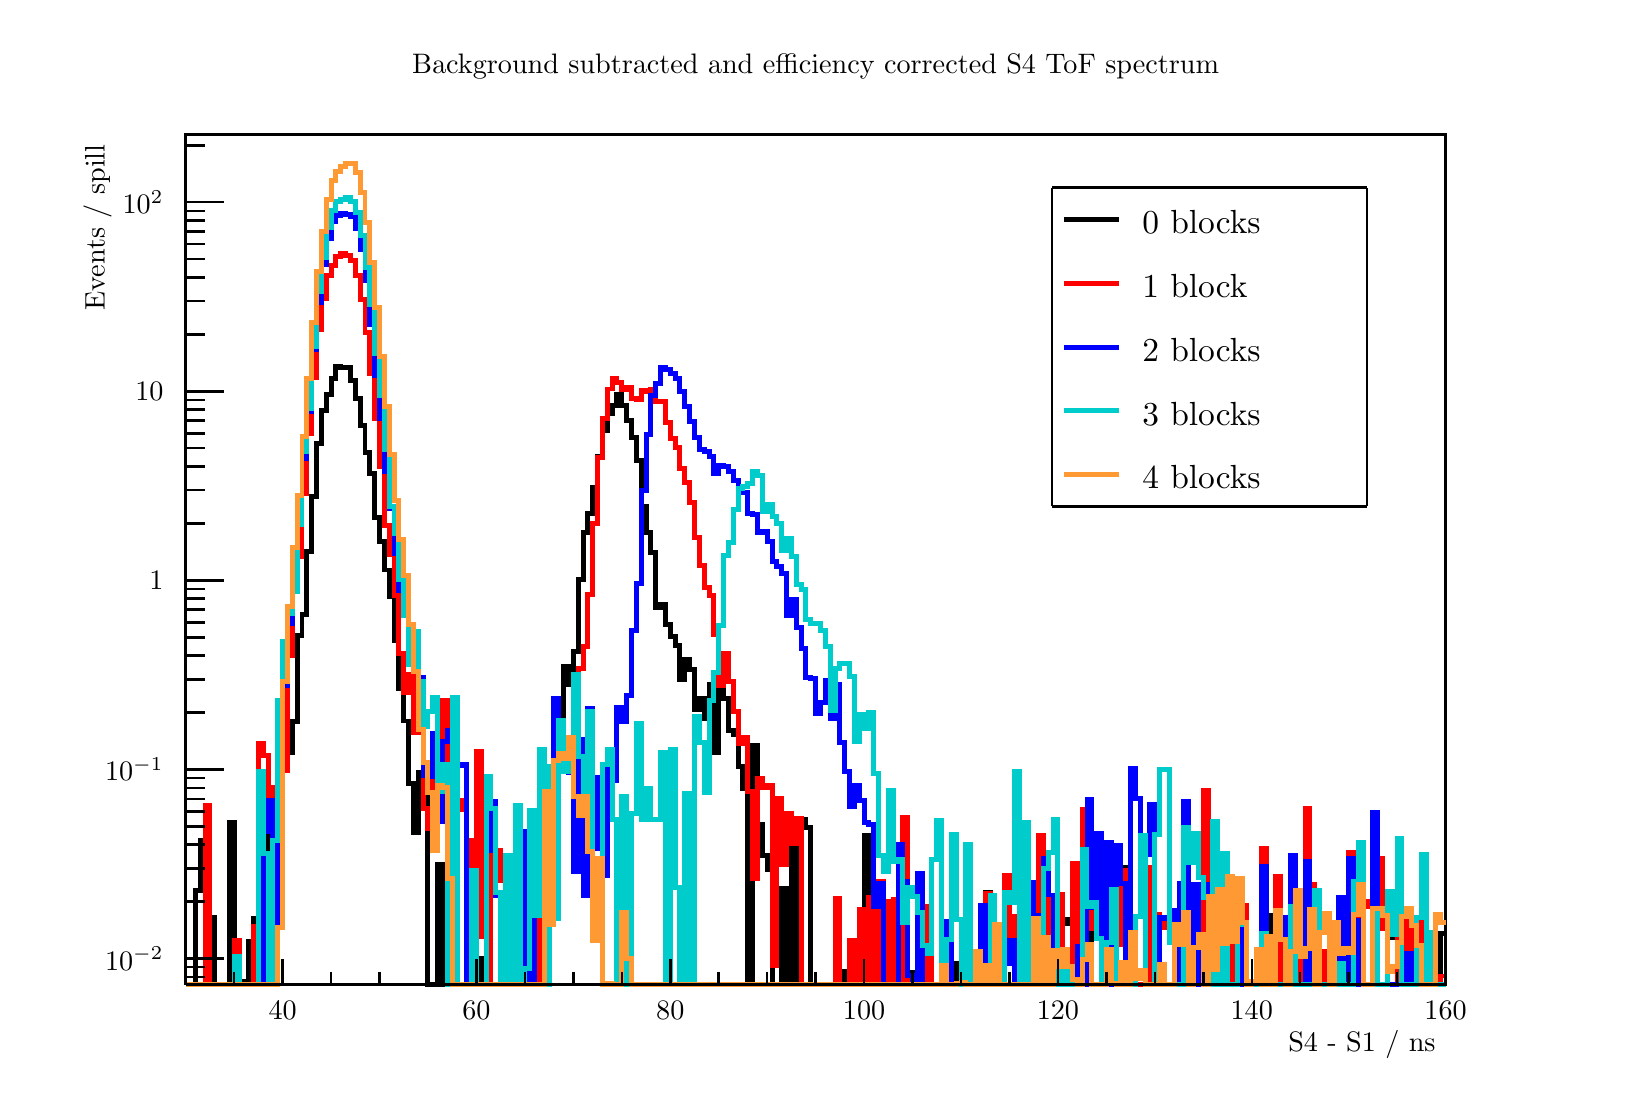
\begin{tikzpicture}
\pgfdeclareplotmark{cross} {
\pgfpathmoveto{\pgfpoint{-0.3\pgfplotmarksize}{\pgfplotmarksize}}
\pgfpathlineto{\pgfpoint{+0.3\pgfplotmarksize}{\pgfplotmarksize}}
\pgfpathlineto{\pgfpoint{+0.3\pgfplotmarksize}{0.3\pgfplotmarksize}}
\pgfpathlineto{\pgfpoint{+1\pgfplotmarksize}{0.3\pgfplotmarksize}}
\pgfpathlineto{\pgfpoint{+1\pgfplotmarksize}{-0.3\pgfplotmarksize}}
\pgfpathlineto{\pgfpoint{+0.3\pgfplotmarksize}{-0.3\pgfplotmarksize}}
\pgfpathlineto{\pgfpoint{+0.3\pgfplotmarksize}{-1.\pgfplotmarksize}}
\pgfpathlineto{\pgfpoint{-0.3\pgfplotmarksize}{-1.\pgfplotmarksize}}
\pgfpathlineto{\pgfpoint{-0.3\pgfplotmarksize}{-0.3\pgfplotmarksize}}
\pgfpathlineto{\pgfpoint{-1.\pgfplotmarksize}{-0.3\pgfplotmarksize}}
\pgfpathlineto{\pgfpoint{-1.\pgfplotmarksize}{0.3\pgfplotmarksize}}
\pgfpathlineto{\pgfpoint{-0.3\pgfplotmarksize}{0.3\pgfplotmarksize}}
\pgfpathclose
\pgfusepathqstroke
}
\pgfdeclareplotmark{cross*} {
\pgfpathmoveto{\pgfpoint{-0.3\pgfplotmarksize}{\pgfplotmarksize}}
\pgfpathlineto{\pgfpoint{+0.3\pgfplotmarksize}{\pgfplotmarksize}}
\pgfpathlineto{\pgfpoint{+0.3\pgfplotmarksize}{0.3\pgfplotmarksize}}
\pgfpathlineto{\pgfpoint{+1\pgfplotmarksize}{0.3\pgfplotmarksize}}
\pgfpathlineto{\pgfpoint{+1\pgfplotmarksize}{-0.3\pgfplotmarksize}}
\pgfpathlineto{\pgfpoint{+0.3\pgfplotmarksize}{-0.3\pgfplotmarksize}}
\pgfpathlineto{\pgfpoint{+0.3\pgfplotmarksize}{-1.\pgfplotmarksize}}
\pgfpathlineto{\pgfpoint{-0.3\pgfplotmarksize}{-1.\pgfplotmarksize}}
\pgfpathlineto{\pgfpoint{-0.3\pgfplotmarksize}{-0.3\pgfplotmarksize}}
\pgfpathlineto{\pgfpoint{-1.\pgfplotmarksize}{-0.3\pgfplotmarksize}}
\pgfpathlineto{\pgfpoint{-1.\pgfplotmarksize}{0.3\pgfplotmarksize}}
\pgfpathlineto{\pgfpoint{-0.3\pgfplotmarksize}{0.3\pgfplotmarksize}}
\pgfpathclose
\pgfusepathqfillstroke
}
\pgfdeclareplotmark{newstar} {
\pgfpathmoveto{\pgfqpoint{0pt}{\pgfplotmarksize}}
\pgfpathlineto{\pgfqpointpolar{44}{0.5\pgfplotmarksize}}
\pgfpathlineto{\pgfqpointpolar{18}{\pgfplotmarksize}}
\pgfpathlineto{\pgfqpointpolar{-20}{0.5\pgfplotmarksize}}
\pgfpathlineto{\pgfqpointpolar{-54}{\pgfplotmarksize}}
\pgfpathlineto{\pgfqpointpolar{-90}{0.5\pgfplotmarksize}}
\pgfpathlineto{\pgfqpointpolar{234}{\pgfplotmarksize}}
\pgfpathlineto{\pgfqpointpolar{198}{0.5\pgfplotmarksize}}
\pgfpathlineto{\pgfqpointpolar{162}{\pgfplotmarksize}}
\pgfpathlineto{\pgfqpointpolar{134}{0.5\pgfplotmarksize}}
\pgfpathclose
\pgfusepathqstroke
}
\pgfdeclareplotmark{newstar*} {
\pgfpathmoveto{\pgfqpoint{0pt}{\pgfplotmarksize}}
\pgfpathlineto{\pgfqpointpolar{44}{0.5\pgfplotmarksize}}
\pgfpathlineto{\pgfqpointpolar{18}{\pgfplotmarksize}}
\pgfpathlineto{\pgfqpointpolar{-20}{0.5\pgfplotmarksize}}
\pgfpathlineto{\pgfqpointpolar{-54}{\pgfplotmarksize}}
\pgfpathlineto{\pgfqpointpolar{-90}{0.5\pgfplotmarksize}}
\pgfpathlineto{\pgfqpointpolar{234}{\pgfplotmarksize}}
\pgfpathlineto{\pgfqpointpolar{198}{0.5\pgfplotmarksize}}
\pgfpathlineto{\pgfqpointpolar{162}{\pgfplotmarksize}}
\pgfpathlineto{\pgfqpointpolar{134}{0.5\pgfplotmarksize}}
\pgfpathclose
\pgfusepathqfillstroke
}
\definecolor{c}{rgb}{1,1,1};
\draw [color=c, fill=c] (0,0) rectangle (20,13.4957);
\draw [color=c, fill=c] (2,1.34957) rectangle (18,12.1461);
\definecolor{c}{rgb}{0,0,0};
\draw [c,line width=0.9] (2,1.34957) -- (2,12.1461) -- (18,12.1461) -- (18,1.34957) -- (2,1.34957);
\definecolor{c}{rgb}{1,1,1};
\draw [color=c, fill=c] (2,1.34957) rectangle (18,12.1461);
\definecolor{c}{rgb}{0,0,0};
\draw [c,line width=0.9] (2,1.34957) -- (2,12.1461) -- (18,12.1461) -- (18,1.34957) -- (2,1.34957);
\definecolor{c}{rgb}{0,0,0.6};
\draw [c,line width=0.9] (2,1.34957) -- (2.06154,1.34957) -- (2.06154,1.34957) -- (2.12308,1.34957) -- (2.12308,1.34957) -- (2.18462,1.34957) -- (2.18462,1.34957) -- (2.24615,1.34957) -- (2.24615,1.34957) -- (2.30769,1.34957) -- (2.30769,1.34957) --
 (2.36923,1.34957) -- (2.36923,1.34957) -- (2.43077,1.34957) -- (2.43077,1.34957) -- (2.49231,1.34957) -- (2.49231,1.34957) -- (2.55385,1.34957) -- (2.55385,1.34957) -- (2.61538,1.34957) -- (2.61538,1.34957) -- (2.67692,1.34957) -- (2.67692,1.34957)
 -- (2.73846,1.34957) -- (2.73846,1.34957) -- (2.8,1.34957) -- (2.8,1.34957) -- (2.86154,1.34957) -- (2.86154,1.34957) -- (2.92308,1.34957) -- (2.92308,1.34957) -- (2.98462,1.34957) -- (2.98462,1.34957) -- (3.04615,1.34957) -- (3.04615,1.34957) --
 (3.10769,1.34957) -- (3.10769,1.34957) -- (3.16923,1.34957) -- (3.16923,1.34957) -- (3.23077,1.34957) -- (3.23077,1.34957) -- (3.29231,1.34957) -- (3.29231,1.34957) -- (3.35385,1.34957) -- (3.35385,1.34957) -- (3.41538,1.34957) -- (3.41538,1.34957)
 -- (3.47692,1.34957) -- (3.47692,1.34957) -- (3.53846,1.34957) -- (3.53846,1.34957) -- (3.6,1.34957) -- (3.6,1.34957) -- (3.66154,1.34957) -- (3.66154,1.34957) -- (3.72308,1.34957) -- (3.72308,1.34957) -- (3.78462,1.34957) -- (3.78462,1.34957) --
 (3.84615,1.34957) -- (3.84615,1.34957) -- (3.90769,1.34957) -- (3.90769,1.34957) -- (3.96923,1.34957) -- (3.96923,1.34957) -- (4.03077,1.34957) -- (4.03077,1.34957) -- (4.09231,1.34957) -- (4.09231,1.34957) -- (4.15385,1.34957) -- (4.15385,1.34957)
 -- (4.21538,1.34957) -- (4.21538,1.34957) -- (4.27692,1.34957) -- (4.27692,1.34957) -- (4.33846,1.34957) -- (4.33846,1.34957) -- (4.4,1.34957) -- (4.4,1.34957) -- (4.46154,1.34957) -- (4.46154,1.34957) -- (4.52308,1.34957) -- (4.52308,1.34957) --
 (4.58462,1.34957) -- (4.58462,1.34957) -- (4.64615,1.34957) -- (4.64615,1.34957) -- (4.70769,1.34957) -- (4.70769,1.34957) -- (4.76923,1.34957) -- (4.76923,1.34957) -- (4.83077,1.34957) -- (4.83077,1.34957) -- (4.89231,1.34957) -- (4.89231,1.34957)
 -- (4.95385,1.34957) -- (4.95385,1.34957) -- (5.01538,1.34957) -- (5.01538,1.34957) -- (5.07692,1.34957) -- (5.07692,1.34957) -- (5.13846,1.34957) -- (5.13846,1.34957) -- (5.2,1.34957) -- (5.2,1.34957) -- (5.26154,1.34957) -- (5.26154,1.34957) --
 (5.32308,1.34957) -- (5.32308,1.34957) -- (5.38462,1.34957) -- (5.38462,1.34957) -- (5.44615,1.34957) -- (5.44615,1.34957) -- (5.50769,1.34957) -- (5.50769,1.34957) -- (5.56923,1.34957) -- (5.56923,1.34957) -- (5.63077,1.34957) -- (5.63077,1.34957)
 -- (5.69231,1.34957) -- (5.69231,1.34957) -- (5.75385,1.34957) -- (5.75385,1.34957) -- (5.81538,1.34957) -- (5.81538,1.34957) -- (5.87692,1.34957) -- (5.87692,1.34957) -- (5.93846,1.34957) -- (5.93846,1.34957) -- (6,1.34957) -- (6,1.34957) --
 (6.06154,1.34957) -- (6.06154,1.34957) -- (6.12308,1.34957) -- (6.12308,1.34957) -- (6.18462,1.34957) -- (6.18462,1.34957) -- (6.24615,1.34957) -- (6.24615,1.34957) -- (6.30769,1.34957) -- (6.30769,1.34957) -- (6.36923,1.34957) -- (6.36923,1.34957)
 -- (6.43077,1.34957) -- (6.43077,1.34957) -- (6.49231,1.34957) -- (6.49231,1.34957) -- (6.55385,1.34957) -- (6.55385,1.34957) -- (6.61538,1.34957) -- (6.61538,1.34957) -- (6.67692,1.34957) -- (6.67692,1.34957) -- (6.73846,1.34957) --
 (6.73846,1.34957) -- (6.8,1.34957) -- (6.8,1.34957) -- (6.86154,1.34957) -- (6.86154,1.34957) -- (6.92308,1.34957) -- (6.92308,1.34957) -- (6.98462,1.34957) -- (6.98462,1.34957) -- (7.04615,1.34957) -- (7.04615,1.34957) -- (7.10769,1.34957) --
 (7.10769,1.34957) -- (7.16923,1.34957) -- (7.16923,1.34957) -- (7.23077,1.34957) -- (7.23077,1.34957) -- (7.29231,1.34957) -- (7.29231,1.34957) -- (7.35385,1.34957) -- (7.35385,1.34957) -- (7.41538,1.34957) -- (7.41538,1.34957) -- (7.47692,1.34957)
 -- (7.47692,1.34957) -- (7.53846,1.34957) -- (7.53846,1.34957) -- (7.6,1.34957) -- (7.6,1.34957) -- (7.66154,1.34957) -- (7.66154,1.34957) -- (7.72308,1.34957) -- (7.72308,1.34957) -- (7.78462,1.34957) -- (7.78462,1.34957) -- (7.84615,1.34957) --
 (7.84615,1.34957) -- (7.90769,1.34957) -- (7.90769,1.34957) -- (7.96923,1.34957) -- (7.96923,1.34957) -- (8.03077,1.34957) -- (8.03077,1.34957) -- (8.09231,1.34957) -- (8.09231,1.34957) -- (8.15385,1.34957) -- (8.15385,1.34957) -- (8.21538,1.34957)
 -- (8.21538,1.34957) -- (8.27692,1.34957) -- (8.27692,1.34957) -- (8.33846,1.34957) -- (8.33846,1.34957) -- (8.4,1.34957) -- (8.4,1.34957) -- (8.46154,1.34957) -- (8.46154,1.34957) -- (8.52308,1.34957) -- (8.52308,1.34957) -- (8.58462,1.34957) --
 (8.58462,1.34957) -- (8.64615,1.34957) -- (8.64615,1.34957) -- (8.70769,1.34957) -- (8.70769,1.34957) -- (8.76923,1.34957) -- (8.76923,1.34957) -- (8.83077,1.34957) -- (8.83077,1.34957) -- (8.89231,1.34957) -- (8.89231,1.34957) -- (8.95385,1.34957)
 -- (8.95385,1.34957) -- (9.01538,1.34957) -- (9.01538,1.34957) -- (9.07692,1.34957) -- (9.07692,1.34957) -- (9.13846,1.34957) -- (9.13846,1.34957) -- (9.2,1.34957) -- (9.2,1.34957) -- (9.26154,1.34957) -- (9.26154,1.34957) -- (9.32308,1.34957) --
 (9.32308,1.34957) -- (9.38461,1.34957) -- (9.38461,1.34957) -- (9.44615,1.34957) -- (9.44615,1.34957) -- (9.50769,1.34957) -- (9.50769,1.34957) -- (9.56923,1.34957) -- (9.56923,1.34957) -- (9.63077,1.34957) -- (9.63077,1.34957) -- (9.69231,1.34957)
 -- (9.69231,1.34957) -- (9.75385,1.34957) -- (9.75385,1.34957) -- (9.81538,1.34957) -- (9.81538,1.34957) -- (9.87692,1.34957) -- (9.87692,1.34957) -- (9.93846,1.34957) -- (9.93846,1.34957) -- (10,1.34957) -- (10,1.34957) -- (10.0615,1.34957) --
 (10.0615,1.34957) -- (10.1231,1.34957) -- (10.1231,1.34957) -- (10.1846,1.34957) -- (10.1846,1.34957) -- (10.2462,1.34957) -- (10.2462,1.34957) -- (10.3077,1.34957) -- (10.3077,1.34957) -- (10.3692,1.34957) -- (10.3692,1.34957) -- (10.4308,1.34957)
 -- (10.4308,1.34957) -- (10.4923,1.34957) -- (10.4923,1.34957) -- (10.5538,1.34957) -- (10.5538,1.34957) -- (10.6154,1.34957) -- (10.6154,1.34957) -- (10.6769,1.34957) -- (10.6769,1.34957) -- (10.7385,1.34957) -- (10.7385,1.34957) -- (10.8,1.34957)
 -- (10.8,1.34957) -- (10.8615,1.34957) -- (10.8615,1.34957) -- (10.9231,1.34957) -- (10.9231,1.34957) -- (10.9846,1.34957) -- (10.9846,1.34957) -- (11.0462,1.34957) -- (11.0462,1.34957) -- (11.1077,1.34957) -- (11.1077,1.34957) -- (11.1692,1.34957)
 -- (11.1692,1.34957) -- (11.2308,1.34957) -- (11.2308,1.34957) -- (11.2923,1.34957) -- (11.2923,1.34957) -- (11.3538,1.34957) -- (11.3538,1.34957) -- (11.4154,1.34957) -- (11.4154,1.34957) -- (11.4769,1.34957) -- (11.4769,1.34957) --
 (11.5385,1.34957) -- (11.5385,1.34957) -- (11.6,1.34957) -- (11.6,1.34957) -- (11.6615,1.34957) -- (11.6615,1.34957) -- (11.7231,1.34957) -- (11.7231,1.34957) -- (11.7846,1.34957) -- (11.7846,1.34957) -- (11.8462,1.34957) -- (11.8462,1.34957) --
 (11.9077,1.34957) -- (11.9077,1.34957) -- (11.9692,1.34957) -- (11.9692,1.34957) -- (12.0308,1.34957) -- (12.0308,1.34957) -- (12.0923,1.34957) -- (12.0923,1.34957) -- (12.1538,1.34957) -- (12.1538,1.34957) -- (12.2154,1.34957) -- (12.2154,1.34957)
 -- (12.2769,1.34957) -- (12.2769,1.34957) -- (12.3385,1.34957) -- (12.3385,1.34957) -- (12.4,1.34957) -- (12.4,1.34957) -- (12.4615,1.34957) -- (12.4615,1.34957) -- (12.5231,1.34957) -- (12.5231,1.34957) -- (12.5846,1.34957) -- (12.5846,1.34957) --
 (12.6462,1.34957) -- (12.6462,1.34957) -- (12.7077,1.34957) -- (12.7077,1.34957) -- (12.7692,1.34957) -- (12.7692,1.34957) -- (12.8308,1.34957) -- (12.8308,1.34957) -- (12.8923,1.34957) -- (12.8923,1.34957) -- (12.9538,1.34957) -- (12.9538,1.34957)
 -- (13.0154,1.34957) -- (13.0154,1.34957) -- (13.0769,1.34957) -- (13.0769,1.34957) -- (13.1385,1.34957) -- (13.1385,1.34957) -- (13.2,1.34957) -- (13.2,1.34957) -- (13.2615,1.34957) -- (13.2615,1.34957) -- (13.3231,1.34957) -- (13.3231,1.34957) --
 (13.3846,1.34957) -- (13.3846,1.34957) -- (13.4462,1.34957) -- (13.4462,1.34957) -- (13.5077,1.34957) -- (13.5077,1.34957) -- (13.5692,1.34957) -- (13.5692,1.34957) -- (13.6308,1.34957) -- (13.6308,1.34957) -- (13.6923,1.34957) -- (13.6923,1.34957)
 -- (13.7538,1.34957) -- (13.7538,1.34957) -- (13.8154,1.34957) -- (13.8154,1.34957) -- (13.8769,1.34957) -- (13.8769,1.34957) -- (13.9385,1.34957) -- (13.9385,1.34957) -- (14,1.34957) -- (14,1.34957) -- (14.0615,1.34957) -- (14.0615,1.34957) --
 (14.1231,1.34957) -- (14.1231,1.34957) -- (14.1846,1.34957) -- (14.1846,1.34957) -- (14.2462,1.34957) -- (14.2462,1.34957) -- (14.3077,1.34957) -- (14.3077,1.34957) -- (14.3692,1.34957) -- (14.3692,1.34957) -- (14.4308,1.34957) -- (14.4308,1.34957)
 -- (14.4923,1.34957) -- (14.4923,1.34957) -- (14.5538,1.34957) -- (14.5538,1.34957) -- (14.6154,1.34957) -- (14.6154,1.34957) -- (14.6769,1.34957) -- (14.6769,1.34957) -- (14.7385,1.34957) -- (14.7385,1.34957) -- (14.8,1.34957) -- (14.8,1.34957) --
 (14.8615,1.34957) -- (14.8615,1.34957) -- (14.9231,1.34957) -- (14.9231,1.34957) -- (14.9846,1.34957) -- (14.9846,1.34957) -- (15.0462,1.34957) -- (15.0462,1.34957) -- (15.1077,1.34957) -- (15.1077,1.34957) -- (15.1692,1.34957) -- (15.1692,1.34957)
 -- (15.2308,1.34957) -- (15.2308,1.34957) -- (15.2923,1.34957) -- (15.2923,1.34957) -- (15.3538,1.34957) -- (15.3538,1.34957) -- (15.4154,1.34957) -- (15.4154,1.34957) -- (15.4769,1.34957) -- (15.4769,1.34957) -- (15.5385,1.34957) --
 (15.5385,1.34957) -- (15.6,1.34957) -- (15.6,1.34957) -- (15.6615,1.34957) -- (15.6615,1.34957) -- (15.7231,1.34957) -- (15.7231,1.34957) -- (15.7846,1.34957) -- (15.7846,1.34957) -- (15.8462,1.34957) -- (15.8462,1.34957) -- (15.9077,1.34957) --
 (15.9077,1.34957) -- (15.9692,1.34957) -- (15.9692,1.34957) -- (16.0308,1.34957) -- (16.0308,1.34957) -- (16.0923,1.34957) -- (16.0923,1.34957) -- (16.1538,1.34957) -- (16.1538,1.34957) -- (16.2154,1.34957) -- (16.2154,1.34957) -- (16.2769,1.34957)
 -- (16.2769,1.34957) -- (16.3385,1.34957) -- (16.3385,1.34957) -- (16.4,1.34957) -- (16.4,1.34957) -- (16.4615,1.34957) -- (16.4615,1.34957) -- (16.5231,1.34957) -- (16.5231,1.34957) -- (16.5846,1.34957) -- (16.5846,1.34957) -- (16.6462,1.34957) --
 (16.6462,1.34957) -- (16.7077,1.34957) -- (16.7077,1.34957) -- (16.7692,1.34957) -- (16.7692,1.34957) -- (16.8308,1.34957) -- (16.8308,1.34957) -- (16.8923,1.34957) -- (16.8923,1.34957) -- (16.9538,1.34957) -- (16.9538,1.34957) -- (17.0154,1.34957)
 -- (17.0154,1.34957) -- (17.0769,1.34957) -- (17.0769,1.34957) -- (17.1385,1.34957) -- (17.1385,1.34957) -- (17.2,1.34957) -- (17.2,1.34957) -- (17.2615,1.34957) -- (17.2615,1.34957) -- (17.3231,1.34957) -- (17.3231,1.34957) -- (17.3846,1.34957) --
 (17.3846,1.34957) -- (17.4462,1.34957) -- (17.4462,1.34957) -- (17.5077,1.34957) -- (17.5077,1.34957) -- (17.5692,1.34957) -- (17.5692,1.34957) -- (17.6308,1.34957) -- (17.6308,1.34957) -- (17.6923,1.34957) -- (17.6923,1.34957) -- (17.7538,1.34957)
 -- (17.7538,1.34957) -- (17.8154,1.34957) -- (17.8154,1.34957) -- (17.8769,1.34957) -- (17.8769,1.34957) -- (17.9385,1.34957) -- (17.9385,1.34957) -- (18,1.34957);
\definecolor{c}{rgb}{0,0,0};
\draw [c,line width=0.9] (2,1.34957) -- (18,1.34957);
\draw [c,line width=0.9] (3.23077,1.67347) -- (3.23077,1.34957);
\draw [c,line width=0.9] (3.84615,1.51152) -- (3.84615,1.34957);
\draw [c,line width=0.9] (4.46154,1.51152) -- (4.46154,1.34957);
\draw [c,line width=0.9] (5.07692,1.51152) -- (5.07692,1.34957);
\draw [c,line width=0.9] (5.69231,1.67347) -- (5.69231,1.34957);
\draw [c,line width=0.9] (6.30769,1.51152) -- (6.30769,1.34957);
\draw [c,line width=0.9] (6.92308,1.51152) -- (6.92308,1.34957);
\draw [c,line width=0.9] (7.53846,1.51152) -- (7.53846,1.34957);
\draw [c,line width=0.9] (8.15385,1.67347) -- (8.15385,1.34957);
\draw [c,line width=0.9] (8.76923,1.51152) -- (8.76923,1.34957);
\draw [c,line width=0.9] (9.38461,1.51152) -- (9.38461,1.34957);
\draw [c,line width=0.9] (10,1.51152) -- (10,1.34957);
\draw [c,line width=0.9] (10.6154,1.67347) -- (10.6154,1.34957);
\draw [c,line width=0.9] (11.2308,1.51152) -- (11.2308,1.34957);
\draw [c,line width=0.9] (11.8462,1.51152) -- (11.8462,1.34957);
\draw [c,line width=0.9] (12.4615,1.51152) -- (12.4615,1.34957);
\draw [c,line width=0.9] (13.0769,1.67347) -- (13.0769,1.34957);
\draw [c,line width=0.9] (13.6923,1.51152) -- (13.6923,1.34957);
\draw [c,line width=0.9] (14.3077,1.51152) -- (14.3077,1.34957);
\draw [c,line width=0.9] (14.9231,1.51152) -- (14.9231,1.34957);
\draw [c,line width=0.9] (15.5385,1.67347) -- (15.5385,1.34957);
\draw [c,line width=0.9] (16.1538,1.51152) -- (16.1538,1.34957);
\draw [c,line width=0.9] (16.7692,1.51152) -- (16.7692,1.34957);
\draw [c,line width=0.9] (17.3846,1.51152) -- (17.3846,1.34957);
\draw [c,line width=0.9] (18,1.67347) -- (18,1.34957);
\draw [c,line width=0.9] (3.23077,1.67347) -- (3.23077,1.34957);
\draw [c,line width=0.9] (2.61538,1.51152) -- (2.61538,1.34957);
\draw [c,line width=0.9] (2,1.51152) -- (2,1.34957);
\draw [anchor=base] (3.23077,0.904212) node[scale=1.01821, color=c, rotate=0]{40};
\draw [anchor=base] (5.69231,0.904212) node[scale=1.01821, color=c, rotate=0]{60};
\draw [anchor=base] (8.15385,0.904212) node[scale=1.01821, color=c, rotate=0]{80};
\draw [anchor=base] (10.6154,0.904212) node[scale=1.01821, color=c, rotate=0]{100};
\draw [anchor=base] (13.0769,0.904212) node[scale=1.01821, color=c, rotate=0]{120};
\draw [anchor=base] (15.5385,0.904212) node[scale=1.01821, color=c, rotate=0]{140};
\draw [anchor=base] (18,0.904212) node[scale=1.01821, color=c, rotate=0]{160};
\draw [anchor= east] (18,0.593811) node[scale=1.01821, color=c, rotate=0]{ S4 - S1 / ns};
\draw [c,line width=0.9] (2,1.34957) -- (2,12.1461);
\draw [c,line width=0.9] (2.24,1.44788) -- (2,1.44788);
\draw [c,line width=0.9] (2.24,1.57071) -- (2,1.57071);
\draw [c,line width=0.9] (2.48,1.68059) -- (2,1.68059);
\draw [anchor= east] (1.844,1.68059) node[scale=1.01821, color=c, rotate=0]{$10^{-2}$};
\draw [c,line width=0.9] (2.24,2.40344) -- (2,2.40344);
\draw [c,line width=0.9] (2.24,2.82629) -- (2,2.82629);
\draw [c,line width=0.9] (2.24,3.1263) -- (2,3.1263);
\draw [c,line width=0.9] (2.24,3.35901) -- (2,3.35901);
\draw [c,line width=0.9] (2.24,3.54914) -- (2,3.54914);
\draw [c,line width=0.9] (2.24,3.7099) -- (2,3.7099);
\draw [c,line width=0.9] (2.24,3.84916) -- (2,3.84916);
\draw [c,line width=0.9] (2.24,3.97199) -- (2,3.97199);
\draw [c,line width=0.9] (2.48,4.08186) -- (2,4.08186);
\draw [anchor= east] (1.844,4.08186) node[scale=1.01821, color=c, rotate=0]{$10^{-1}$};
\draw [c,line width=0.9] (2.24,4.80472) -- (2,4.80472);
\draw [c,line width=0.9] (2.24,5.22756) -- (2,5.22756);
\draw [c,line width=0.9] (2.24,5.52758) -- (2,5.52758);
\draw [c,line width=0.9] (2.24,5.76028) -- (2,5.76028);
\draw [c,line width=0.9] (2.24,5.95042) -- (2,5.95042);
\draw [c,line width=0.9] (2.24,6.11118) -- (2,6.11118);
\draw [c,line width=0.9] (2.24,6.25043) -- (2,6.25043);
\draw [c,line width=0.9] (2.24,6.37327) -- (2,6.37327);
\draw [c,line width=0.9] (2.48,6.48314) -- (2,6.48314);
\draw [anchor= east] (1.844,6.48314) node[scale=1.01821, color=c, rotate=0]{1};
\draw [c,line width=0.9] (2.24,7.206) -- (2,7.206);
\draw [c,line width=0.9] (2.24,7.62884) -- (2,7.62884);
\draw [c,line width=0.9] (2.24,7.92885) -- (2,7.92885);
\draw [c,line width=0.9] (2.24,8.16156) -- (2,8.16156);
\draw [c,line width=0.9] (2.24,8.3517) -- (2,8.3517);
\draw [c,line width=0.9] (2.24,8.51246) -- (2,8.51246);
\draw [c,line width=0.9] (2.24,8.65171) -- (2,8.65171);
\draw [c,line width=0.9] (2.24,8.77454) -- (2,8.77454);
\draw [c,line width=0.9] (2.48,8.88442) -- (2,8.88442);
\draw [anchor= east] (1.844,8.88442) node[scale=1.01821, color=c, rotate=0]{10};
\draw [c,line width=0.9] (2.24,9.60728) -- (2,9.60728);
\draw [c,line width=0.9] (2.24,10.0301) -- (2,10.0301);
\draw [c,line width=0.9] (2.24,10.3301) -- (2,10.3301);
\draw [c,line width=0.9] (2.24,10.5628) -- (2,10.5628);
\draw [c,line width=0.9] (2.24,10.753) -- (2,10.753);
\draw [c,line width=0.9] (2.24,10.9137) -- (2,10.9137);
\draw [c,line width=0.9] (2.24,11.053) -- (2,11.053);
\draw [c,line width=0.9] (2.24,11.1758) -- (2,11.1758);
\draw [c,line width=0.9] (2.48,11.2857) -- (2,11.2857);
\draw [anchor= east] (1.844,11.2857) node[scale=1.01821, color=c, rotate=0]{$10^{2}$};
\draw [c,line width=0.9] (2.24,12.0086) -- (2,12.0086);
\draw [anchor= east] (0.88,12.1461) node[scale=1.01821, color=c, rotate=90]{ Events / spill};
\draw [c,line width=1.8] (2,1.34957) -- (2.06154,1.34957) -- (2.06154,1.34957) -- (2.12308,1.34957) -- (2.12308,2.53951) -- (2.18462,2.53951) -- (2.18462,3.17729) -- (2.24615,3.17729) -- (2.24615,1.34957) -- (2.30769,1.34957) -- (2.30769,2.20144) --
 (2.36923,2.20144) -- (2.36923,1.34957) -- (2.43077,1.34957) -- (2.43077,1.34957) -- (2.49231,1.34957) -- (2.49231,1.34957) -- (2.55385,1.34957) -- (2.55385,3.40479) -- (2.61538,3.40479) -- (2.61538,1.34957) -- (2.67692,1.34957) -- (2.67692,1.34957)
 -- (2.73846,1.34957) -- (2.73846,1.38687) -- (2.8,1.38687) -- (2.8,1.90133) -- (2.86154,1.90133) -- (2.86154,2.18515) -- (2.92308,2.18515) -- (2.92308,3.61789) -- (2.98462,3.61789) -- (2.98462,3.25403) -- (3.04615,3.25403) -- (3.04615,1.34957) --
 (3.10769,1.34957) -- (3.10769,3.39189) -- (3.16923,3.39189) -- (3.16923,4.13184) -- (3.23077,4.13184) -- (3.23077,4.44884) -- (3.29231,4.44884) -- (3.29231,4.30025) -- (3.35385,4.30025) -- (3.35385,4.68859) -- (3.41538,4.68859) -- (3.41538,5.78092)
 -- (3.47692,5.78092) -- (3.47692,6.05252) -- (3.53846,6.05252) -- (3.53846,6.85477) -- (3.6,6.85477) -- (3.6,7.55269) -- (3.66154,7.55269) -- (3.66154,8.22225) -- (3.72308,8.22225) -- (3.72308,8.64481) -- (3.78462,8.64481) -- (3.78462,8.84179) --
 (3.84615,8.84179) -- (3.84615,9.04392) -- (3.90769,9.04392) -- (3.90769,9.20268) -- (3.96923,9.20268) -- (3.96923,9.18123) -- (4.03077,9.18123) -- (4.03077,9.19048) -- (4.09231,9.19048) -- (4.09231,9.02681) -- (4.15385,9.02681) -- (4.15385,8.78913)
 -- (4.21538,8.78913) -- (4.21538,8.45125) -- (4.27692,8.45125) -- (4.27692,8.10572) -- (4.33846,8.10572) -- (4.33846,7.84076) -- (4.4,7.84076) -- (4.4,7.28435) -- (4.46154,7.28435) -- (4.46154,6.98214) -- (4.52308,6.98214) -- (4.52308,6.61504) --
 (4.58462,6.61504) -- (4.58462,6.27553) -- (4.64615,6.27553) -- (4.64615,5.72202) -- (4.70769,5.72202) -- (4.70769,5.11195) -- (4.76923,5.11195) -- (4.76923,4.69735) -- (4.83077,4.69735) -- (4.83077,3.90316) -- (4.89231,3.90316) -- (4.89231,3.28257)
 -- (4.95385,3.28257) -- (4.95385,4.04247) -- (5.01538,4.04247) -- (5.01538,3.738) -- (5.07692,3.738) -- (5.07692,1.34957) -- (5.13846,1.34957) -- (5.13846,1.34957) -- (5.2,1.34957) -- (5.2,2.87862) -- (5.26154,2.87862) -- (5.26154,1.34957) --
 (5.32308,1.34957) -- (5.32308,2.92743) -- (5.38462,2.92743) -- (5.38462,3.00257) -- (5.44615,3.00257) -- (5.44615,1.34957) -- (5.50769,1.34957) -- (5.50769,1.34957) -- (5.56923,1.34957) -- (5.56923,1.34957) -- (5.63077,1.34957) -- (5.63077,1.34957)
 -- (5.69231,1.34957) -- (5.69231,1.68015) -- (5.75385,1.68015) -- (5.75385,1.34957) -- (5.81538,1.34957) -- (5.81538,2.57343) -- (5.87692,2.57343) -- (5.87692,1.34957) -- (5.93846,1.34957) -- (5.93846,1.34957) -- (6,1.34957) -- (6,1.34957) --
 (6.06154,1.34957) -- (6.06154,1.34957) -- (6.12308,1.34957) -- (6.12308,1.34957) -- (6.18462,1.34957) -- (6.18462,1.34957) -- (6.24615,1.34957) -- (6.24615,2.06003) -- (6.30769,2.06003) -- (6.30769,1.34957) -- (6.36923,1.34957) -- (6.36923,1.34957)
 -- (6.43077,1.34957) -- (6.43077,3.20391) -- (6.49231,3.20391) -- (6.49231,2.17723) -- (6.55385,2.17723) -- (6.55385,3.12456) -- (6.61538,3.12456) -- (6.61538,3.55551) -- (6.67692,3.55551) -- (6.67692,4.3017) -- (6.73846,4.3017) -- (6.73846,4.53853)
 -- (6.8,4.53853) -- (6.8,5.38926) -- (6.86154,5.38926) -- (6.86154,5.16006) -- (6.92308,5.16006) -- (6.92308,5.57801) -- (6.98462,5.57801) -- (6.98462,6.49955) -- (7.04615,6.49955) -- (7.04615,7.08983) -- (7.10769,7.08983) -- (7.10769,7.32942) --
 (7.16923,7.32942) -- (7.16923,7.66242) -- (7.23077,7.66242) -- (7.23077,8.06249) -- (7.29231,8.06249) -- (7.29231,8.38303) -- (7.35385,8.38303) -- (7.35385,8.60368) -- (7.41538,8.60368) -- (7.41538,8.70027) -- (7.47692,8.70027) -- (7.47692,8.84394)
 -- (7.53846,8.84394) -- (7.53846,8.70221) -- (7.6,8.70221) -- (7.6,8.51775) -- (7.66154,8.51775) -- (7.66154,8.29905) -- (7.72308,8.29905) -- (7.72308,8.00204) -- (7.78462,8.00204) -- (7.78462,7.42284) -- (7.84615,7.42284) -- (7.84615,7.09375) --
 (7.90769,7.09375) -- (7.90769,6.83915) -- (7.96923,6.83915) -- (7.96923,6.1409) -- (8.03077,6.1409) -- (8.03077,6.18103) -- (8.09231,6.18103) -- (8.09231,5.92597) -- (8.15385,5.92597) -- (8.15385,5.76712) -- (8.21538,5.76712) -- (8.21538,5.6565) --
 (8.27692,5.6565) -- (8.27692,5.2214) -- (8.33846,5.2214) -- (8.33846,5.48398) -- (8.4,5.48398) -- (8.4,5.35061) -- (8.46154,5.35061) -- (8.46154,4.83908) -- (8.52308,4.83908) -- (8.52308,4.97696) -- (8.58462,4.97696) -- (8.58462,4.72547) --
 (8.64615,4.72547) -- (8.64615,5.16273) -- (8.70769,5.16273) -- (8.70769,4.30101) -- (8.76923,4.30101) -- (8.76923,5.1798) -- (8.83077,5.1798) -- (8.83077,4.98008) -- (8.89231,4.98008) -- (8.89231,4.57223) -- (8.95385,4.57223) -- (8.95385,4.52429) --
 (9.01538,4.52429) -- (9.01538,4.11848) -- (9.07692,4.11848) -- (9.07692,3.84027) -- (9.13846,3.84027) -- (9.13846,1.34957) -- (9.2,1.34957) -- (9.2,4.38175) -- (9.26154,4.38175) -- (9.26154,3.37945) -- (9.32308,3.37945) -- (9.32308,2.98425) --
 (9.38461,2.98425) -- (9.38461,2.81682) -- (9.44615,2.81682) -- (9.44615,1.34957) -- (9.50769,1.34957) -- (9.50769,1.34957) -- (9.56923,1.34957) -- (9.56923,2.56799) -- (9.63077,2.56799) -- (9.63077,1.34957) -- (9.69231,1.34957) -- (9.69231,3.38931)
 -- (9.75385,3.38931) -- (9.75385,1.34957) -- (9.81538,1.34957) -- (9.81538,3.44534) -- (9.87692,3.44534) -- (9.87692,3.34676) -- (9.93846,3.34676) -- (9.93846,1.34957) -- (10,1.34957) -- (10,1.34957) -- (10.0615,1.34957) -- (10.0615,1.34957) --
 (10.1231,1.34957) -- (10.1231,1.34957) -- (10.1846,1.34957) -- (10.1846,1.34957) -- (10.2462,1.34957) -- (10.2462,1.34957) -- (10.3077,1.34957) -- (10.3077,1.51017) -- (10.3692,1.51017) -- (10.3692,1.34957) -- (10.4308,1.34957) -- (10.4308,1.34957)
 -- (10.4923,1.34957) -- (10.4923,1.34957) -- (10.5538,1.34957) -- (10.5538,1.34957) -- (10.6154,1.34957) -- (10.6154,3.2483) -- (10.6769,3.2483) -- (10.6769,1.77041) -- (10.7385,1.77041) -- (10.7385,1.34957) -- (10.8,1.34957) -- (10.8,1.34957) --
 (10.8615,1.34957) -- (10.8615,1.34957) -- (10.9231,1.34957) -- (10.9231,1.34957) -- (10.9846,1.34957) -- (10.9846,1.34957) -- (11.0462,1.34957) -- (11.0462,1.34957) -- (11.1077,1.34957) -- (11.1077,1.34957) -- (11.1692,1.34957) -- (11.1692,1.49969)
 -- (11.2308,1.49969) -- (11.2308,1.34957) -- (11.2923,1.34957) -- (11.2923,1.34957) -- (11.3538,1.34957) -- (11.3538,1.34957) -- (11.4154,1.34957) -- (11.4154,1.34957) -- (11.4769,1.34957) -- (11.4769,1.34957) -- (11.5385,1.34957) --
 (11.5385,1.34957) -- (11.6,1.34957) -- (11.6,1.34957) -- (11.6615,1.34957) -- (11.6615,1.85741) -- (11.7231,1.85741) -- (11.7231,1.34957) -- (11.7846,1.34957) -- (11.7846,1.62176) -- (11.8462,1.62176) -- (11.8462,1.34957) -- (11.9077,1.34957) --
 (11.9077,1.34957) -- (11.9692,1.34957) -- (11.9692,1.35861) -- (12.0308,1.35861) -- (12.0308,1.34957) -- (12.0923,1.34957) -- (12.0923,1.34957) -- (12.1538,1.34957) -- (12.1538,2.52198) -- (12.2154,2.52198) -- (12.2154,1.34957) -- (12.2769,1.34957)
 -- (12.2769,1.34957) -- (12.3385,1.34957) -- (12.3385,1.34957) -- (12.4,1.34957) -- (12.4,1.34957) -- (12.4615,1.34957) -- (12.4615,1.34957) -- (12.5231,1.34957) -- (12.5231,1.78978) -- (12.5846,1.78978) -- (12.5846,1.34957) -- (12.6462,1.34957) --
 (12.6462,1.34957) -- (12.7077,1.34957) -- (12.7077,1.34957) -- (12.7692,1.34957) -- (12.7692,1.34957) -- (12.8308,1.34957) -- (12.8308,1.34957) -- (12.8923,1.34957) -- (12.8923,2.1804) -- (12.9538,2.1804) -- (12.9538,1.34957) -- (13.0154,1.34957) --
 (13.0154,1.34957) -- (13.0769,1.34957) -- (13.0769,1.34957) -- (13.1385,1.34957) -- (13.1385,2.1314) -- (13.2,2.1314) -- (13.2,2.1798) -- (13.2615,2.1798) -- (13.2615,1.34957) -- (13.3231,1.34957) -- (13.3231,1.34957) -- (13.3846,1.34957) --
 (13.3846,1.34957) -- (13.4462,1.34957) -- (13.4462,1.34957) -- (13.5077,1.34957) -- (13.5077,2.64658) -- (13.5692,2.64658) -- (13.5692,2.39108) -- (13.6308,2.39108) -- (13.6308,1.34957) -- (13.6923,1.34957) -- (13.6923,1.34957) -- (13.7538,1.34957)
 -- (13.7538,1.34957) -- (13.8154,1.34957) -- (13.8154,1.34957) -- (13.8769,1.34957) -- (13.8769,1.34957) -- (13.9385,1.34957) -- (13.9385,2.83893) -- (14,2.83893) -- (14,2.11491) -- (14.0615,2.11491) -- (14.0615,1.34957) -- (14.1231,1.34957) --
 (14.1231,1.34957) -- (14.1846,1.34957) -- (14.1846,1.34957) -- (14.2462,1.34957) -- (14.2462,1.34957) -- (14.3077,1.34957) -- (14.3077,1.76693) -- (14.3692,1.76693) -- (14.3692,1.34957) -- (14.4308,1.34957) -- (14.4308,1.34957) -- (14.4923,1.34957)
 -- (14.4923,1.34957) -- (14.5538,1.34957) -- (14.5538,1.34957) -- (14.6154,1.34957) -- (14.6154,1.34957) -- (14.6769,1.34957) -- (14.6769,1.34957) -- (14.7385,1.34957) -- (14.7385,2.3037) -- (14.8,2.3037) -- (14.8,1.34957) -- (14.8615,1.34957) --
 (14.8615,1.34957) -- (14.9231,1.34957) -- (14.9231,1.34957) -- (14.9846,1.34957) -- (14.9846,1.34957) -- (15.0462,1.34957) -- (15.0462,1.34957) -- (15.1077,1.34957) -- (15.1077,1.34957) -- (15.1692,1.34957) -- (15.1692,1.34957) -- (15.2308,1.34957)
 -- (15.2308,1.34957) -- (15.2923,1.34957) -- (15.2923,2.5842) -- (15.3538,2.5842) -- (15.3538,1.34957) -- (15.4154,1.34957) -- (15.4154,1.34957) -- (15.4769,1.34957) -- (15.4769,1.34957) -- (15.5385,1.34957) -- (15.5385,1.34957) -- (15.6,1.34957) --
 (15.6,1.34957) -- (15.6615,1.34957) -- (15.6615,1.34957) -- (15.7231,1.34957) -- (15.7231,1.34957) -- (15.7846,1.34957) -- (15.7846,2.22124) -- (15.8462,2.22124) -- (15.8462,1.34957) -- (15.9077,1.34957) -- (15.9077,1.95528) -- (15.9692,1.95528) --
 (15.9692,1.34957) -- (16.0308,1.34957) -- (16.0308,1.34957) -- (16.0923,1.34957) -- (16.0923,1.34957) -- (16.1538,1.34957) -- (16.1538,1.34957) -- (16.2154,1.34957) -- (16.2154,1.34957) -- (16.2769,1.34957) -- (16.2769,1.34957) -- (16.3385,1.34957)
 -- (16.3385,1.34957) -- (16.4,1.34957) -- (16.4,1.34957) -- (16.4615,1.34957) -- (16.4615,1.34957) -- (16.5231,1.34957) -- (16.5231,1.34957) -- (16.5846,1.34957) -- (16.5846,1.34957) -- (16.6462,1.34957) -- (16.6462,1.34957) -- (16.7077,1.34957) --
 (16.7077,1.34957) -- (16.7692,1.34957) -- (16.7692,1.34957) -- (16.8308,1.34957) -- (16.8308,1.34957) -- (16.8923,1.34957) -- (16.8923,1.34957) -- (16.9538,1.34957) -- (16.9538,1.34957) -- (17.0154,1.34957) -- (17.0154,1.34957) -- (17.0769,1.34957)
 -- (17.0769,1.34957) -- (17.1385,1.34957) -- (17.1385,1.34957) -- (17.2,1.34957) -- (17.2,1.34957) -- (17.2615,1.34957) -- (17.2615,1.95386) -- (17.3231,1.95386) -- (17.3231,2.36022) -- (17.3846,2.36022) -- (17.3846,1.34957) -- (17.4462,1.34957) --
 (17.4462,1.34957) -- (17.5077,1.34957) -- (17.5077,1.34957) -- (17.5692,1.34957) -- (17.5692,1.34957) -- (17.6308,1.34957) -- (17.6308,1.34957) -- (17.6923,1.34957) -- (17.6923,1.34957) -- (17.7538,1.34957) -- (17.7538,1.34957) -- (17.8154,1.34957)
 -- (17.8154,1.34957) -- (17.8769,1.34957) -- (17.8769,1.34957) -- (17.9385,1.34957) -- (17.9385,1.99545) -- (18,1.99545);
\definecolor{c}{rgb}{1,0,0};
\draw [c,line width=1.8] (2,1.34957) -- (2.06154,1.34957) -- (2.06154,1.34957) -- (2.12308,1.34957) -- (2.12308,1.34957) -- (2.18462,1.34957) -- (2.18462,1.34957) -- (2.24615,1.34957) -- (2.24615,3.62161) -- (2.30769,3.62161) -- (2.30769,1.34957) --
 (2.36923,1.34957) -- (2.36923,1.34957) -- (2.43077,1.34957) -- (2.43077,1.34957) -- (2.49231,1.34957) -- (2.49231,1.34957) -- (2.55385,1.34957) -- (2.55385,1.34957) -- (2.61538,1.34957) -- (2.61538,1.91584) -- (2.67692,1.91584) -- (2.67692,1.34957)
 -- (2.73846,1.34957) -- (2.73846,1.34957) -- (2.8,1.34957) -- (2.8,1.34957) -- (2.86154,1.34957) -- (2.86154,2.08919) -- (2.92308,2.08919) -- (2.92308,4.4145) -- (2.98462,4.4145) -- (2.98462,4.26301) -- (3.04615,4.26301) -- (3.04615,3.61527) --
 (3.10769,3.61527) -- (3.10769,3.85244) -- (3.16923,3.85244) -- (3.16923,4.38046) -- (3.23077,4.38046) -- (3.23077,4.07497) -- (3.29231,4.07497) -- (3.29231,5.53218) -- (3.35385,5.53218) -- (3.35385,6.47699) -- (3.41538,6.47699) -- (3.41538,6.78566)
 -- (3.47692,6.78566) -- (3.47692,7.59064) -- (3.53846,7.59064) -- (3.53846,8.35131) -- (3.6,8.35131) -- (3.6,9.06486) -- (3.66154,9.06486) -- (3.66154,9.66563) -- (3.72308,9.66563) -- (3.72308,10.0693) -- (3.78462,10.0693) -- (3.78462,10.3609) --
 (3.84615,10.3609) -- (3.84615,10.4829) -- (3.90769,10.4829) -- (3.90769,10.5931) -- (3.96923,10.5931) -- (3.96923,10.6313) -- (4.03077,10.6313) -- (4.03077,10.6118) -- (4.09231,10.6118) -- (4.09231,10.5475) -- (4.15385,10.5475) -- (4.15385,10.3521)
 -- (4.21538,10.3521) -- (4.21538,10.0547) -- (4.27692,10.0547) -- (4.27692,9.63751) -- (4.33846,9.63751) -- (4.33846,9.11073) -- (4.4,9.11073) -- (4.4,8.53346) -- (4.46154,8.53346) -- (4.46154,7.93332) -- (4.52308,7.93332) -- (4.52308,7.18344) --
 (4.58462,7.18344) -- (4.58462,6.81416) -- (4.64615,6.81416) -- (4.64615,6.29079) -- (4.70769,6.29079) -- (4.70769,5.55098) -- (4.76923,5.55098) -- (4.76923,5.06016) -- (4.83077,5.06016) -- (4.83077,5.28237) -- (4.89231,5.28237) -- (4.89231,4.54614)
 -- (4.95385,4.54614) -- (4.95385,4.60508) -- (5.01538,4.60508) -- (5.01538,3.59119) -- (5.07692,3.59119) -- (5.07692,3.33771) -- (5.13846,3.33771) -- (5.13846,4.31041) -- (5.2,4.31041) -- (5.2,4.02115) -- (5.26154,4.02115) -- (5.26154,4.96132) --
 (5.32308,4.96132) -- (5.32308,3.64012) -- (5.38462,3.64012) -- (5.38462,3.17982) -- (5.44615,3.17982) -- (5.44615,3.57534) -- (5.50769,3.57534) -- (5.50769,3.68747) -- (5.56923,3.68747) -- (5.56923,3.18227) -- (5.63077,3.18227) -- (5.63077,1.34957)
 -- (5.69231,1.34957) -- (5.69231,4.30999) -- (5.75385,4.30999) -- (5.75385,1.95629) -- (5.81538,1.95629) -- (5.81538,1.34957) -- (5.87692,1.34957) -- (5.87692,3.12297) -- (5.93846,3.12297) -- (5.93846,3.05309) -- (6,3.05309) -- (6,2.6762) --
 (6.06154,2.6762) -- (6.06154,2.30519) -- (6.12308,2.30519) -- (6.12308,1.80391) -- (6.18462,1.80391) -- (6.18462,2.48112) -- (6.24615,2.48112) -- (6.24615,1.34957) -- (6.30769,1.34957) -- (6.30769,1.34957) -- (6.36923,1.34957) -- (6.36923,1.34957)
 -- (6.43077,1.34957) -- (6.43077,1.34957) -- (6.49231,1.34957) -- (6.49231,3.16213) -- (6.55385,3.16213) -- (6.55385,2.75945) -- (6.61538,2.75945) -- (6.61538,4.00308) -- (6.67692,4.00308) -- (6.67692,4.33309) -- (6.73846,4.33309) --
 (6.73846,4.39393) -- (6.8,4.39393) -- (6.8,4.21582) -- (6.86154,4.21582) -- (6.86154,4.19149) -- (6.92308,4.19149) -- (6.92308,4.95959) -- (6.98462,4.95959) -- (6.98462,5.36654) -- (7.04615,5.36654) -- (7.04615,5.64098) -- (7.10769,5.64098) --
 (7.10769,6.29884) -- (7.16923,6.29884) -- (7.16923,7.20416) -- (7.23077,7.20416) -- (7.23077,8.04797) -- (7.29231,8.04797) -- (7.29231,8.54071) -- (7.35385,8.54071) -- (7.35385,8.91385) -- (7.41538,8.91385) -- (7.41538,9.04707) -- (7.47692,9.04707)
 -- (7.47692,8.99555) -- (7.53846,8.99555) -- (7.53846,8.90349) -- (7.6,8.90349) -- (7.6,8.93229) -- (7.66154,8.93229) -- (7.66154,8.79037) -- (7.72308,8.79037) -- (7.72308,8.77626) -- (7.78462,8.77626) -- (7.78462,8.89617) -- (7.84615,8.89617) --
 (7.84615,8.87567) -- (7.90769,8.87567) -- (7.90769,8.90707) -- (7.96923,8.90707) -- (7.96923,8.75828) -- (8.03077,8.75828) -- (8.03077,8.74976) -- (8.09231,8.74976) -- (8.09231,8.48745) -- (8.15385,8.48745) -- (8.15385,8.28347) -- (8.21538,8.28347)
 -- (8.21538,8.1741) -- (8.27692,8.1741) -- (8.27692,7.90876) -- (8.33846,7.90876) -- (8.33846,7.7225) -- (8.4,7.7225) -- (8.4,7.47768) -- (8.46154,7.47768) -- (8.46154,7.03069) -- (8.52308,7.03069) -- (8.52308,6.67147) -- (8.58462,6.67147) --
 (8.58462,6.39729) -- (8.64615,6.39729) -- (8.64615,6.29457) -- (8.70769,6.29457) -- (8.70769,5.80017) -- (8.76923,5.80017) -- (8.76923,5.15044) -- (8.83077,5.15044) -- (8.83077,5.55743) -- (8.89231,5.55743) -- (8.89231,5.20087) -- (8.95385,5.20087)
 -- (8.95385,4.81439) -- (9.01538,4.81439) -- (9.01538,4.40663) -- (9.07692,4.40663) -- (9.07692,4.48419) -- (9.13846,4.48419) -- (9.13846,3.80072) -- (9.2,3.80072) -- (9.2,2.70315) -- (9.26154,2.70315) -- (9.26154,3.96834) -- (9.32308,3.96834) --
 (9.32308,3.84722) -- (9.38461,3.84722) -- (9.38461,3.8737) -- (9.44615,3.8737) -- (9.44615,1.59699) -- (9.50769,1.59699) -- (9.50769,3.71748) -- (9.56923,3.71748) -- (9.56923,2.87557) -- (9.63077,2.87557) -- (9.63077,3.52477) -- (9.69231,3.52477) --
 (9.69231,3.1478) -- (9.75385,3.1478) -- (9.75385,3.46079) -- (9.81538,3.46079) -- (9.81538,1.34957) -- (9.87692,1.34957) -- (9.87692,1.34957) -- (9.93846,1.34957) -- (9.93846,1.34957) -- (10,1.34957) -- (10,1.34957) -- (10.0615,1.34957) --
 (10.0615,1.34957) -- (10.1231,1.34957) -- (10.1231,1.34957) -- (10.1846,1.34957) -- (10.1846,1.34957) -- (10.2462,1.34957) -- (10.2462,2.44947) -- (10.3077,2.44947) -- (10.3077,1.34957) -- (10.3692,1.34957) -- (10.3692,1.34957) -- (10.4308,1.34957)
 -- (10.4308,1.90882) -- (10.4923,1.90882) -- (10.4923,1.34957) -- (10.5538,1.34957) -- (10.5538,2.3036) -- (10.6154,2.3036) -- (10.6154,1.34957) -- (10.6769,1.34957) -- (10.6769,2.46027) -- (10.7385,2.46027) -- (10.7385,1.34957) -- (10.8,1.34957) --
 (10.8,2.662) -- (10.8615,2.662) -- (10.8615,2.40261) -- (10.9231,2.40261) -- (10.9231,1.34957) -- (10.9846,1.34957) -- (10.9846,2.43248) -- (11.0462,2.43248) -- (11.0462,1.34957) -- (11.1077,1.34957) -- (11.1077,3.47275) -- (11.1692,3.47275) --
 (11.1692,1.34957) -- (11.2308,1.34957) -- (11.2308,1.34957) -- (11.2923,1.34957) -- (11.2923,1.34957) -- (11.3538,1.34957) -- (11.3538,1.34957) -- (11.4154,1.34957) -- (11.4154,2.34399) -- (11.4769,2.34399) -- (11.4769,1.34957) -- (11.5385,1.34957)
 -- (11.5385,1.34957) -- (11.6,1.34957) -- (11.6,1.34957) -- (11.6615,1.34957) -- (11.6615,1.34957) -- (11.7231,1.34957) -- (11.7231,1.34957) -- (11.7846,1.34957) -- (11.7846,1.34957) -- (11.8462,1.34957) -- (11.8462,1.34957) -- (11.9077,1.34957) --
 (11.9077,2.01152) -- (11.9692,2.01152) -- (11.9692,1.3899) -- (12.0308,1.3899) -- (12.0308,1.34957) -- (12.0923,1.34957) -- (12.0923,1.34957) -- (12.1538,1.34957) -- (12.1538,2.50694) -- (12.2154,2.50694) -- (12.2154,1.34957) -- (12.2769,1.34957) --
 (12.2769,1.34957) -- (12.3385,1.34957) -- (12.3385,1.34957) -- (12.4,1.34957) -- (12.4,2.73973) -- (12.4615,2.73973) -- (12.4615,1.83266) -- (12.5231,1.83266) -- (12.5231,2.21319) -- (12.5846,2.21319) -- (12.5846,1.34957) -- (12.6462,1.34957) --
 (12.6462,3.10848) -- (12.7077,3.10848) -- (12.7077,2.30703) -- (12.7692,2.30703) -- (12.7692,1.34957) -- (12.8308,1.34957) -- (12.8308,3.24106) -- (12.8923,3.24106) -- (12.8923,2.5724) -- (12.9538,2.5724) -- (12.9538,1.34957) -- (13.0154,1.34957) --
 (13.0154,1.34957) -- (13.0769,1.34957) -- (13.0769,2.4991) -- (13.1385,2.4991) -- (13.1385,1.34957) -- (13.2,1.34957) -- (13.2,1.34957) -- (13.2615,1.34957) -- (13.2615,2.88411) -- (13.3231,2.88411) -- (13.3231,1.67493) -- (13.3846,1.67493) --
 (13.3846,3.56834) -- (13.4462,3.56834) -- (13.4462,2.05624) -- (13.5077,2.05624) -- (13.5077,2.30361) -- (13.5692,2.30361) -- (13.5692,2.77081) -- (13.6308,2.77081) -- (13.6308,2.6865) -- (13.6923,2.6865) -- (13.6923,1.34957) -- (13.7538,1.34957) --
 (13.7538,2.6628) -- (13.8154,2.6628) -- (13.8154,1.86128) -- (13.8769,1.86128) -- (13.8769,2.79514) -- (13.9385,2.79514) -- (13.9385,2.38322) -- (14,2.38322) -- (14,1.80875) -- (14.0615,1.80875) -- (14.0615,1.34957) -- (14.1231,1.34957) --
 (14.1231,1.34957) -- (14.1846,1.34957) -- (14.1846,1.34957) -- (14.2462,1.34957) -- (14.2462,2.84199) -- (14.3077,2.84199) -- (14.3077,2.24454) -- (14.3692,2.24454) -- (14.3692,2.14648) -- (14.4308,2.14648) -- (14.4308,2.07437) -- (14.4923,2.07437)
 -- (14.4923,2.28133) -- (14.5538,2.28133) -- (14.5538,1.34957) -- (14.6154,1.34957) -- (14.6154,1.34957) -- (14.6769,1.34957) -- (14.6769,2.00143) -- (14.7385,2.00143) -- (14.7385,1.34957) -- (14.8,1.34957) -- (14.8,1.882) -- (14.8615,1.882) --
 (14.8615,1.3765) -- (14.9231,1.3765) -- (14.9231,3.81445) -- (14.9846,3.81445) -- (14.9846,1.65267) -- (15.0462,1.65267) -- (15.0462,1.34957) -- (15.1077,1.34957) -- (15.1077,2.58712) -- (15.1692,2.58712) -- (15.1692,1.61622) -- (15.2308,1.61622) --
 (15.2308,1.34957) -- (15.2923,1.34957) -- (15.2923,2.23174) -- (15.3538,2.23174) -- (15.3538,1.34957) -- (15.4154,1.34957) -- (15.4154,2.3591) -- (15.4769,2.3591) -- (15.4769,1.34957) -- (15.5385,1.34957) -- (15.5385,1.34957) -- (15.6,1.34957) --
 (15.6,1.34957) -- (15.6615,1.34957) -- (15.6615,3.07734) -- (15.7231,3.07734) -- (15.7231,1.34957) -- (15.7846,1.34957) -- (15.7846,1.34957) -- (15.8462,1.34957) -- (15.8462,2.71798) -- (15.9077,2.71798) -- (15.9077,1.36019) -- (15.9692,1.36019) --
 (15.9692,1.86205) -- (16.0308,1.86205) -- (16.0308,1.6721) -- (16.0923,1.6721) -- (16.0923,1.34957) -- (16.1538,1.34957) -- (16.1538,1.80862) -- (16.2154,1.80862) -- (16.2154,3.58636) -- (16.2769,3.58636) -- (16.2769,2.61896) -- (16.3385,2.61896) --
 (16.3385,1.86351) -- (16.4,1.86351) -- (16.4,1.34957) -- (16.4615,1.34957) -- (16.4615,1.76757) -- (16.5231,1.76757) -- (16.5231,1.96406) -- (16.5846,1.96406) -- (16.5846,1.34957) -- (16.6462,1.34957) -- (16.6462,1.34957) -- (16.7077,1.34957) --
 (16.7077,1.34957) -- (16.7692,1.34957) -- (16.7692,3.02213) -- (16.8308,3.02213) -- (16.8308,1.34957) -- (16.8923,1.34957) -- (16.8923,2.62715) -- (16.9538,2.62715) -- (16.9538,2.40865) -- (17.0154,2.40865) -- (17.0154,2.34677) -- (17.0769,2.34677)
 -- (17.0769,1.72071) -- (17.1385,1.72071) -- (17.1385,2.95211) -- (17.2,2.95211) -- (17.2,2.06272) -- (17.2615,2.06272) -- (17.2615,1.34957) -- (17.3231,1.34957) -- (17.3231,1.34957) -- (17.3846,1.34957) -- (17.3846,2.25591) -- (17.4462,2.25591) --
 (17.4462,1.34957) -- (17.5077,1.34957) -- (17.5077,2.3061) -- (17.5692,2.3061) -- (17.5692,1.34957) -- (17.6308,1.34957) -- (17.6308,1.74036) -- (17.6923,1.74036) -- (17.6923,2.26535) -- (17.7538,2.26535) -- (17.7538,1.34957) -- (17.8154,1.34957) --
 (17.8154,1.48232) -- (17.8769,1.48232) -- (17.8769,1.34957) -- (17.9385,1.34957) -- (17.9385,1.45908) -- (18,1.45908);
\definecolor{c}{rgb}{0,0,1};
\draw [c,line width=1.8] (2,1.34957) -- (2.06154,1.34957) -- (2.06154,1.34957) -- (2.12308,1.34957) -- (2.12308,1.34957) -- (2.18462,1.34957) -- (2.18462,1.34957) -- (2.24615,1.34957) -- (2.24615,1.34957) -- (2.30769,1.34957) -- (2.30769,1.34957) --
 (2.36923,1.34957) -- (2.36923,1.34957) -- (2.43077,1.34957) -- (2.43077,1.34957) -- (2.49231,1.34957) -- (2.49231,1.34957) -- (2.55385,1.34957) -- (2.55385,1.34957) -- (2.61538,1.34957) -- (2.61538,1.34957) -- (2.67692,1.34957) -- (2.67692,1.34957)
 -- (2.73846,1.34957) -- (2.73846,1.34957) -- (2.8,1.34957) -- (2.8,1.34957) -- (2.86154,1.34957) -- (2.86154,1.34957) -- (2.92308,1.34957) -- (2.92308,1.34957) -- (2.98462,1.34957) -- (2.98462,3.29051) -- (3.04615,3.29051) -- (3.04615,3.68893) --
 (3.10769,3.68893) -- (3.10769,1.34957) -- (3.16923,1.34957) -- (3.16923,4.28821) -- (3.23077,4.28821) -- (3.23077,5.15094) -- (3.29231,5.15094) -- (3.29231,5.93267) -- (3.35385,5.93267) -- (3.35385,6.37765) -- (3.41538,6.37765) -- (3.41538,7.28467)
 -- (3.47692,7.28467) -- (3.47692,8.02529) -- (3.53846,8.02529) -- (3.53846,8.63203) -- (3.6,8.63203) -- (3.6,9.41846) -- (3.66154,9.41846) -- (3.66154,10.0182) -- (3.72308,10.0182) -- (3.72308,10.4944) -- (3.78462,10.4944) -- (3.78462,10.8294) --
 (3.84615,10.8294) -- (3.84615,11.038) -- (3.90769,11.038) -- (3.90769,11.1169) -- (3.96923,11.1169) -- (3.96923,11.1476) -- (4.03077,11.1476) -- (4.03077,11.1356) -- (4.09231,11.1356) -- (4.09231,11.1) -- (4.15385,11.1) -- (4.15385,10.9513) --
 (4.21538,10.9513) -- (4.21538,10.6838) -- (4.27692,10.6838) -- (4.27692,10.295) -- (4.33846,10.295) -- (4.33846,9.73657) -- (4.4,9.73657) -- (4.4,9.08337) -- (4.46154,9.08337) -- (4.46154,8.53774) -- (4.52308,8.53774) -- (4.52308,7.86205) --
 (4.58462,7.86205) -- (4.58462,7.3994) -- (4.64615,7.3994) -- (4.64615,6.82154) -- (4.70769,6.82154) -- (4.70769,6.35785) -- (4.76923,6.35785) -- (4.76923,6.12188) -- (4.83077,6.12188) -- (4.83077,5.47372) -- (4.89231,5.47372) -- (4.89231,5.43871) --
 (4.95385,5.43871) -- (4.95385,5.25157) -- (5.01538,5.25157) -- (5.01538,4.00659) -- (5.07692,4.00659) -- (5.07692,3.99543) -- (5.13846,3.99543) -- (5.13846,4.53245) -- (5.2,4.53245) -- (5.2,3.42408) -- (5.26154,3.42408) -- (5.26154,4.44117) --
 (5.32308,4.44117) -- (5.32308,4.58218) -- (5.38462,4.58218) -- (5.38462,3.62478) -- (5.44615,3.62478) -- (5.44615,4.1299) -- (5.50769,4.1299) -- (5.50769,4.14519) -- (5.56923,4.14519) -- (5.56923,1.34957) -- (5.63077,1.34957) -- (5.63077,1.86408) --
 (5.69231,1.86408) -- (5.69231,1.34957) -- (5.75385,1.34957) -- (5.75385,1.34957) -- (5.81538,1.34957) -- (5.81538,3.05834) -- (5.87692,3.05834) -- (5.87692,3.6729) -- (5.93846,3.6729) -- (5.93846,2.48051) -- (6,2.48051) -- (6,1.34957) --
 (6.06154,1.34957) -- (6.06154,1.97477) -- (6.12308,1.97477) -- (6.12308,2.48418) -- (6.18462,2.48418) -- (6.18462,3.09956) -- (6.24615,3.09956) -- (6.24615,1.34957) -- (6.30769,1.34957) -- (6.30769,3.28997) -- (6.36923,3.28997) -- (6.36923,1.34957)
 -- (6.43077,1.34957) -- (6.43077,3.10082) -- (6.49231,3.10082) -- (6.49231,3.58845) -- (6.55385,3.58845) -- (6.55385,4.02208) -- (6.61538,4.02208) -- (6.61538,4.00178) -- (6.67692,4.00178) -- (6.67692,4.98382) -- (6.73846,4.98382) --
 (6.73846,4.4141) -- (6.8,4.4141) -- (6.8,4.41556) -- (6.86154,4.41556) -- (6.86154,4.04753) -- (6.92308,4.04753) -- (6.92308,2.78924) -- (6.98462,2.78924) -- (6.98462,4.46738) -- (7.04615,4.46738) -- (7.04615,2.48258) -- (7.10769,2.48258) --
 (7.10769,4.85063) -- (7.16923,4.85063) -- (7.16923,3.08343) -- (7.23077,3.08343) -- (7.23077,3.98083) -- (7.29231,3.98083) -- (7.29231,2.73571) -- (7.35385,2.73571) -- (7.35385,4.17283) -- (7.41538,4.17283) -- (7.41538,3.94391) -- (7.47692,3.94391)
 -- (7.47692,4.87495) -- (7.53846,4.87495) -- (7.53846,4.69383) -- (7.6,4.69383) -- (7.6,5.02686) -- (7.66154,5.02686) -- (7.66154,5.85076) -- (7.72308,5.85076) -- (7.72308,6.43917) -- (7.78462,6.43917) -- (7.78462,7.63053) -- (7.84615,7.63053) --
 (7.84615,8.3334) -- (7.90769,8.3334) -- (7.90769,8.83265) -- (7.96923,8.83265) -- (7.96923,8.9788) -- (8.03077,8.9788) -- (8.03077,9.18449) -- (8.09231,9.18449) -- (8.09231,9.16597) -- (8.15385,9.16597) -- (8.15385,9.10673) -- (8.21538,9.10673) --
 (8.21538,9.04145) -- (8.27692,9.04145) -- (8.27692,8.87912) -- (8.33846,8.87912) -- (8.33846,8.69676) -- (8.4,8.69676) -- (8.4,8.49598) -- (8.46154,8.49598) -- (8.46154,8.30037) -- (8.52308,8.30037) -- (8.52308,8.15047) -- (8.58462,8.15047) --
 (8.58462,8.12396) -- (8.64615,8.12396) -- (8.64615,8.05734) -- (8.70769,8.05734) -- (8.70769,7.8378) -- (8.76923,7.8378) -- (8.76923,7.94572) -- (8.83077,7.94572) -- (8.83077,7.9304) -- (8.89231,7.9304) -- (8.89231,7.86301) -- (8.95385,7.86301) --
 (8.95385,7.75066) -- (9.01538,7.75066) -- (9.01538,7.67871) -- (9.07692,7.67871) -- (9.07692,7.59875) -- (9.13846,7.59875) -- (9.13846,7.33155) -- (9.2,7.33155) -- (9.2,7.31381) -- (9.26154,7.31381) -- (9.26154,7.09328) -- (9.32308,7.09328) --
 (9.32308,7.10565) -- (9.38461,7.10565) -- (9.38461,6.97914) -- (9.44615,6.97914) -- (9.44615,6.72166) -- (9.50769,6.72166) -- (9.50769,6.65636) -- (9.56923,6.65636) -- (9.56923,6.57006) -- (9.63077,6.57006) -- (9.63077,6.03422) -- (9.69231,6.03422)
 -- (9.69231,6.2368) -- (9.75385,6.2368) -- (9.75385,5.88655) -- (9.81538,5.88655) -- (9.81538,5.62243) -- (9.87692,5.62243) -- (9.87692,5.24821) -- (9.93846,5.24821) -- (9.93846,5.23351) -- (10,5.23351) -- (10,4.78734) -- (10.0615,4.78734) --
 (10.0615,4.93274) -- (10.1231,4.93274) -- (10.1231,5.21384) -- (10.1846,5.21384) -- (10.1846,4.73089) -- (10.2462,4.73089) -- (10.2462,5.1642) -- (10.3077,5.1642) -- (10.3077,4.42478) -- (10.3692,4.42478) -- (10.3692,4.06077) -- (10.4308,4.06077) --
 (10.4308,3.61722) -- (10.4923,3.61722) -- (10.4923,3.88312) -- (10.5538,3.88312) -- (10.5538,3.68252) -- (10.6154,3.68252) -- (10.6154,3.40537) -- (10.6769,3.40537) -- (10.6769,3.387) -- (10.7385,3.387) -- (10.7385,2.34682) -- (10.8,2.34682) --
 (10.8,2.63814) -- (10.8615,2.63814) -- (10.8615,1.35742) -- (10.9231,1.35742) -- (10.9231,1.34957) -- (10.9846,1.34957) -- (10.9846,1.34957) -- (11.0462,1.34957) -- (11.0462,3.13251) -- (11.1077,3.13251) -- (11.1077,2.65781) -- (11.1692,2.65781) --
 (11.1692,1.46766) -- (11.2308,1.46766) -- (11.2308,1.34957) -- (11.2923,1.34957) -- (11.2923,2.76639) -- (11.3538,2.76639) -- (11.3538,1.34957) -- (11.4154,1.34957) -- (11.4154,1.34957) -- (11.4769,1.34957) -- (11.4769,1.34957) -- (11.5385,1.34957)
 -- (11.5385,1.34957) -- (11.6,1.34957) -- (11.6,1.34957) -- (11.6615,1.34957) -- (11.6615,2.15294) -- (11.7231,2.15294) -- (11.7231,1.34957) -- (11.7846,1.34957) -- (11.7846,1.34957) -- (11.8462,1.34957) -- (11.8462,1.34957) -- (11.9077,1.34957) --
 (11.9077,2.75726) -- (11.9692,2.75726) -- (11.9692,1.34957) -- (12.0308,1.34957) -- (12.0308,1.34957) -- (12.0923,1.34957) -- (12.0923,2.35242) -- (12.1538,2.35242) -- (12.1538,1.34957) -- (12.2154,1.34957) -- (12.2154,1.34957) -- (12.2769,1.34957)
 -- (12.2769,1.34957) -- (12.3385,1.34957) -- (12.3385,1.34957) -- (12.4,1.34957) -- (12.4,1.61413) -- (12.4615,1.61413) -- (12.4615,1.90884) -- (12.5231,1.90884) -- (12.5231,1.34957) -- (12.5846,1.34957) -- (12.5846,1.34957) -- (12.6462,1.34957) --
 (12.6462,1.34957) -- (12.7077,1.34957) -- (12.7077,2.64661) -- (12.7692,2.64661) -- (12.7692,2.22352) -- (12.8308,2.22352) -- (12.8308,1.34957) -- (12.8923,1.34957) -- (12.8923,2.95341) -- (12.9538,2.95341) -- (12.9538,2.48758) -- (13.0154,2.48758)
 -- (13.0154,1.34957) -- (13.0769,1.34957) -- (13.0769,1.34957) -- (13.1385,1.34957) -- (13.1385,1.34957) -- (13.2,1.34957) -- (13.2,1.34957) -- (13.2615,1.34957) -- (13.2615,1.34957) -- (13.3231,1.34957) -- (13.3231,1.83197) -- (13.3846,1.83197) --
 (13.3846,1.34957) -- (13.4462,1.34957) -- (13.4462,3.70482) -- (13.5077,3.70482) -- (13.5077,2.33077) -- (13.5692,2.33077) -- (13.5692,3.26415) -- (13.6308,3.26415) -- (13.6308,1.34957) -- (13.6923,1.34957) -- (13.6923,3.15032) -- (13.7538,3.15032)
 -- (13.7538,1.34957) -- (13.8154,1.34957) -- (13.8154,3.11584) -- (13.8769,3.11584) -- (13.8769,2.6384) -- (13.9385,2.6384) -- (13.9385,1.34957) -- (14,1.34957) -- (14,4.09451) -- (14.0615,4.09451) -- (14.0615,3.7082) -- (14.1231,3.7082) --
 (14.1231,2.97135) -- (14.1846,2.97135) -- (14.1846,2.99872) -- (14.2462,2.99872) -- (14.2462,3.63961) -- (14.3077,3.63961) -- (14.3077,1.34957) -- (14.3692,1.34957) -- (14.3692,2.20689) -- (14.4308,2.20689) -- (14.4308,2.18937) -- (14.4923,2.18937)
 -- (14.4923,2.28567) -- (14.5538,2.28567) -- (14.5538,1.34957) -- (14.6154,1.34957) -- (14.6154,2.62885) -- (14.6769,2.62885) -- (14.6769,3.67226) -- (14.7385,3.67226) -- (14.7385,1.34957) -- (14.8,1.34957) -- (14.8,2.62698) -- (14.8615,2.62698) --
 (14.8615,1.34957) -- (14.9231,1.34957) -- (14.9231,1.34957) -- (14.9846,1.34957) -- (14.9846,2.6209) -- (15.0462,2.6209) -- (15.0462,1.34957) -- (15.1077,1.34957) -- (15.1077,1.34957) -- (15.1692,1.34957) -- (15.1692,1.34957) -- (15.2308,1.34957) --
 (15.2308,1.34957) -- (15.2923,1.34957) -- (15.2923,1.34957) -- (15.3538,1.34957) -- (15.3538,2.18089) -- (15.4154,2.18089) -- (15.4154,1.34957) -- (15.4769,1.34957) -- (15.4769,1.34957) -- (15.5385,1.34957) -- (15.5385,1.34957) -- (15.6,1.34957) --
 (15.6,1.34957) -- (15.6615,1.34957) -- (15.6615,2.84814) -- (15.7231,2.84814) -- (15.7231,1.34957) -- (15.7846,1.34957) -- (15.7846,1.34957) -- (15.8462,1.34957) -- (15.8462,1.34957) -- (15.9077,1.34957) -- (15.9077,1.34957) -- (15.9692,1.34957) --
 (15.9692,2.2021) -- (16.0308,2.2021) -- (16.0308,2.99518) -- (16.0923,2.99518) -- (16.0923,1.34957) -- (16.1538,1.34957) -- (16.1538,1.34957) -- (16.2154,1.34957) -- (16.2154,2.91431) -- (16.2769,2.91431) -- (16.2769,1.34957) -- (16.3385,1.34957) --
 (16.3385,1.34957) -- (16.4,1.34957) -- (16.4,1.34957) -- (16.4615,1.34957) -- (16.4615,1.34957) -- (16.5231,1.34957) -- (16.5231,1.34957) -- (16.5846,1.34957) -- (16.5846,1.34957) -- (16.6462,1.34957) -- (16.6462,2.45789) -- (16.7077,2.45789) --
 (16.7077,1.34957) -- (16.7692,1.34957) -- (16.7692,2.94853) -- (16.8308,2.94853) -- (16.8308,2.16449) -- (16.8923,2.16449) -- (16.8923,1.34957) -- (16.9538,1.34957) -- (16.9538,1.34957) -- (17.0154,1.34957) -- (17.0154,1.34957) -- (17.0769,1.34957)
 -- (17.0769,3.53441) -- (17.1385,3.53441) -- (17.1385,1.34957) -- (17.2,1.34957) -- (17.2,1.34957) -- (17.2615,1.34957) -- (17.2615,1.34957) -- (17.3231,1.34957) -- (17.3231,1.34957) -- (17.3846,1.34957) -- (17.3846,1.34957) -- (17.4462,1.34957) --
 (17.4462,1.34957) -- (17.5077,1.34957) -- (17.5077,1.74829) -- (17.5692,1.74829) -- (17.5692,1.34957) -- (17.6308,1.34957) -- (17.6308,1.34957) -- (17.6923,1.34957) -- (17.6923,1.34957) -- (17.7538,1.34957) -- (17.7538,1.34957) -- (17.8154,1.34957)
 -- (17.8154,1.34957) -- (17.8769,1.34957) -- (17.8769,1.34957) -- (17.9385,1.34957) -- (17.9385,1.34957) -- (18,1.34957);
\definecolor{c}{rgb}{0,0.8,0.8};
\draw [c,line width=1.8] (2,1.34957) -- (2.06154,1.34957) -- (2.06154,1.34957) -- (2.12308,1.34957) -- (2.12308,1.34957) -- (2.18462,1.34957) -- (2.18462,1.34957) -- (2.24615,1.34957) -- (2.24615,1.34957) -- (2.30769,1.34957) -- (2.30769,1.34957) --
 (2.36923,1.34957) -- (2.36923,1.34957) -- (2.43077,1.34957) -- (2.43077,1.34957) -- (2.49231,1.34957) -- (2.49231,1.34957) -- (2.55385,1.34957) -- (2.55385,1.34957) -- (2.61538,1.34957) -- (2.61538,1.71047) -- (2.67692,1.71047) -- (2.67692,1.34957)
 -- (2.73846,1.34957) -- (2.73846,1.34957) -- (2.8,1.34957) -- (2.8,1.34957) -- (2.86154,1.34957) -- (2.86154,1.34957) -- (2.92308,1.34957) -- (2.92308,4.06174) -- (2.98462,4.06174) -- (2.98462,3.01506) -- (3.04615,3.01506) -- (3.04615,1.34957) --
 (3.10769,1.34957) -- (3.10769,3.17722) -- (3.16923,3.17722) -- (3.16923,4.9609) -- (3.23077,4.9609) -- (3.23077,5.70466) -- (3.29231,5.70466) -- (3.29231,6.05849) -- (3.35385,6.05849) -- (3.35385,6.33865) -- (3.41538,6.33865) -- (3.41538,7.18785) --
 (3.47692,7.18785) -- (3.47692,8.1141) -- (3.53846,8.1141) -- (3.53846,8.66413) -- (3.6,8.66413) -- (3.6,9.45347) -- (3.66154,9.45347) -- (3.66154,10.1577) -- (3.72308,10.1577) -- (3.72308,10.5866) -- (3.78462,10.5866) -- (3.78462,10.9626) --
 (3.84615,10.9626) -- (3.84615,11.1753) -- (3.90769,11.1753) -- (3.90769,11.2902) -- (3.96923,11.2902) -- (3.96923,11.3206) -- (4.03077,11.3206) -- (4.03077,11.3458) -- (4.09231,11.3458) -- (4.09231,11.294) -- (4.15385,11.294) -- (4.15385,11.1572) --
 (4.21538,11.1572) -- (4.21538,10.8618) -- (4.27692,10.8618) -- (4.27692,10.4576) -- (4.33846,10.4576) -- (4.33846,9.99189) -- (4.4,9.99189) -- (4.4,9.3666) -- (4.46154,9.3666) -- (4.46154,8.83022) -- (4.52308,8.83022) -- (4.52308,8.14467) --
 (4.58462,8.14467) -- (4.58462,7.42431) -- (4.64615,7.42431) -- (4.64615,7.07837) -- (4.70769,7.07837) -- (4.70769,6.48851) -- (4.76923,6.48851) -- (4.76923,6.03915) -- (4.83077,6.03915) -- (4.83077,5.42079) -- (4.89231,5.42079) -- (4.89231,5.83319)
 -- (4.95385,5.83319) -- (4.95385,5.19927) -- (5.01538,5.19927) -- (5.01538,4.62224) -- (5.07692,4.62224) -- (5.07692,4.81329) -- (5.13846,4.81329) -- (5.13846,4.9902) -- (5.2,4.9902) -- (5.2,3.80699) -- (5.26154,3.80699) -- (5.26154,4.14304) --
 (5.32308,4.14304) -- (5.32308,1.34957) -- (5.38462,1.34957) -- (5.38462,4.99767) -- (5.44615,4.99767) -- (5.44615,1.34957) -- (5.50769,1.34957) -- (5.50769,1.34957) -- (5.56923,1.34957) -- (5.56923,1.34957) -- (5.63077,1.34957) -- (5.63077,2.79557)
 -- (5.69231,2.79557) -- (5.69231,1.34957) -- (5.75385,1.34957) -- (5.75385,1.34957) -- (5.81538,1.34957) -- (5.81538,3.99746) -- (5.87692,3.99746) -- (5.87692,3.58996) -- (5.93846,3.58996) -- (5.93846,2.52091) -- (6,2.52091) -- (6,1.34957) --
 (6.06154,1.34957) -- (6.06154,2.98529) -- (6.12308,2.98529) -- (6.12308,1.34957) -- (6.18462,1.34957) -- (6.18462,3.62866) -- (6.24615,3.62866) -- (6.24615,1.34957) -- (6.30769,1.34957) -- (6.30769,1.55468) -- (6.36923,1.55468) -- (6.36923,3.55678)
 -- (6.43077,3.55678) -- (6.43077,2.22857) -- (6.49231,2.22857) -- (6.49231,4.33534) -- (6.55385,4.33534) -- (6.55385,1.34957) -- (6.61538,1.34957) -- (6.61538,4.11843) -- (6.67692,4.11843) -- (6.67692,2.19168) -- (6.73846,2.19168) --
 (6.73846,4.69838) -- (6.8,4.69838) -- (6.8,4.05542) -- (6.86154,4.05542) -- (6.86154,4.29809) -- (6.92308,4.29809) -- (6.92308,5.28406) -- (6.98462,5.28406) -- (6.98462,4.25275) -- (7.04615,4.25275) -- (7.04615,3.77857) -- (7.10769,3.77857) --
 (7.10769,4.81512) -- (7.16923,4.81512) -- (7.16923,2.78739) -- (7.23077,2.78739) -- (7.23077,2.86142) -- (7.29231,2.86142) -- (7.29231,4.14941) -- (7.35385,4.14941) -- (7.35385,4.33305) -- (7.41538,4.33305) -- (7.41538,3.45168) -- (7.47692,3.45168)
 -- (7.47692,1.34957) -- (7.53846,1.34957) -- (7.53846,3.73306) -- (7.6,3.73306) -- (7.6,1.34957) -- (7.66154,1.34957) -- (7.66154,3.52885) -- (7.72308,3.52885) -- (7.72308,4.66223) -- (7.78462,4.66223) -- (7.78462,3.44636) -- (7.84615,3.44636) --
 (7.84615,3.83963) -- (7.90769,3.83963) -- (7.90769,3.44675) -- (7.96923,3.44675) -- (7.96923,3.44409) -- (8.03077,3.44409) -- (8.03077,4.29487) -- (8.09231,4.29487) -- (8.09231,1.34957) -- (8.15385,1.34957) -- (8.15385,4.33409) -- (8.21538,4.33409)
 -- (8.21538,2.57723) -- (8.27692,2.57723) -- (8.27692,1.34957) -- (8.33846,1.34957) -- (8.33846,3.77088) -- (8.4,3.77088) -- (8.4,1.40664) -- (8.46154,1.40664) -- (8.46154,4.75353) -- (8.52308,4.75353) -- (8.52308,4.42678) -- (8.58462,4.42678) --
 (8.58462,3.79548) -- (8.64615,3.79548) -- (8.64615,4.95802) -- (8.70769,4.95802) -- (8.70769,5.3107) -- (8.76923,5.3107) -- (8.76923,5.91259) -- (8.83077,5.91259) -- (8.83077,6.80341) -- (8.89231,6.80341) -- (8.89231,6.96943) -- (8.95385,6.96943) --
 (8.95385,7.38138) -- (9.01538,7.38138) -- (9.01538,7.64414) -- (9.07692,7.64414) -- (9.07692,7.6748) -- (9.13846,7.6748) -- (9.13846,7.71549) -- (9.2,7.71549) -- (9.2,7.86268) -- (9.26154,7.86268) -- (9.26154,7.81813) -- (9.32308,7.81813) --
 (9.32308,7.35579) -- (9.38461,7.35579) -- (9.38461,7.44097) -- (9.44615,7.44097) -- (9.44615,7.2955) -- (9.50769,7.2955) -- (9.50769,7.2085) -- (9.56923,7.2085) -- (9.56923,6.86665) -- (9.63077,6.86665) -- (9.63077,7.01397) -- (9.69231,7.01397) --
 (9.69231,6.78075) -- (9.75385,6.78075) -- (9.75385,6.42901) -- (9.81538,6.42901) -- (9.81538,6.37323) -- (9.87692,6.37323) -- (9.87692,5.9822) -- (9.93846,5.9822) -- (9.93846,5.9417) -- (10,5.9417) -- (10,5.93801) -- (10.0615,5.93801) --
 (10.0615,5.84761) -- (10.1231,5.84761) -- (10.1231,5.64199) -- (10.1846,5.64199) -- (10.1846,4.82604) -- (10.2462,4.82604) -- (10.2462,5.35982) -- (10.3077,5.35982) -- (10.3077,5.42692) -- (10.3692,5.42692) -- (10.3692,5.43135) -- (10.4308,5.43135)
 -- (10.4308,5.2665) -- (10.4923,5.2665) -- (10.4923,4.44148) -- (10.5538,4.44148) -- (10.5538,4.78643) -- (10.6154,4.78643) -- (10.6154,4.60031) -- (10.6769,4.60031) -- (10.6769,4.80212) -- (10.7385,4.80212) -- (10.7385,4.0292) -- (10.8,4.0292) --
 (10.8,2.99027) -- (10.8615,2.99027) -- (10.8615,2.78033) -- (10.9231,2.78033) -- (10.9231,3.82121) -- (10.9846,3.82121) -- (10.9846,2.9101) -- (11.0462,2.9101) -- (11.0462,2.93829) -- (11.1077,2.93829) -- (11.1077,2.1355) -- (11.1692,2.1355) --
 (11.1692,2.58633) -- (11.2308,2.58633) -- (11.2308,2.47287) -- (11.2923,2.47287) -- (11.2923,2.2648) -- (11.3538,2.2648) -- (11.3538,1.85154) -- (11.4154,1.85154) -- (11.4154,1.74583) -- (11.4769,1.74583) -- (11.4769,2.93848) -- (11.5385,2.93848) --
 (11.5385,3.43087) -- (11.6,3.43087) -- (11.6,1.34957) -- (11.6615,1.34957) -- (11.6615,1.92623) -- (11.7231,1.92623) -- (11.7231,3.25641) -- (11.7846,3.25641) -- (11.7846,2.17866) -- (11.8462,2.17866) -- (11.8462,1.34957) -- (11.9077,1.34957) --
 (11.9077,3.12966) -- (11.9692,3.12966) -- (11.9692,1.34957) -- (12.0308,1.34957) -- (12.0308,1.34957) -- (12.0923,1.34957) -- (12.0923,1.34957) -- (12.1538,1.34957) -- (12.1538,1.34957) -- (12.2154,1.34957) -- (12.2154,2.47885) -- (12.2769,2.47885)
 -- (12.2769,1.34957) -- (12.3385,1.34957) -- (12.3385,1.34957) -- (12.4,1.34957) -- (12.4,2.52165) -- (12.4615,2.52165) -- (12.4615,2.39072) -- (12.5231,2.39072) -- (12.5231,4.05055) -- (12.5846,4.05055) -- (12.5846,1.34957) -- (12.6462,1.34957) --
 (12.6462,3.40513) -- (12.7077,3.40513) -- (12.7077,1.34957) -- (12.7692,1.34957) -- (12.7692,1.34957) -- (12.8308,1.34957) -- (12.8308,1.34957) -- (12.8923,1.34957) -- (12.8923,2.82909) -- (12.9538,2.82909) -- (12.9538,3.02952) -- (13.0154,3.02952)
 -- (13.0154,3.4442) -- (13.0769,3.4442) -- (13.0769,1.34957) -- (13.1385,1.34957) -- (13.1385,1.79127) -- (13.2,1.79127) -- (13.2,1.34957) -- (13.2615,1.34957) -- (13.2615,1.34957) -- (13.3231,1.34957) -- (13.3231,1.34957) -- (13.3846,1.34957) --
 (13.3846,3.06325) -- (13.4462,3.06325) -- (13.4462,2.33702) -- (13.5077,2.33702) -- (13.5077,2.38695) -- (13.5692,2.38695) -- (13.5692,1.92919) -- (13.6308,1.92919) -- (13.6308,1.34957) -- (13.6923,1.34957) -- (13.6923,1.88563) -- (13.7538,1.88563)
 -- (13.7538,2.55167) -- (13.8154,2.55167) -- (13.8154,1.34957) -- (13.8769,1.34957) -- (13.8769,1.40286) -- (13.9385,1.40286) -- (13.9385,1.34957) -- (14,1.34957) -- (14,1.34957) -- (14.0615,1.34957) -- (14.0615,2.21579) -- (14.1231,2.21579) --
 (14.1231,3.24857) -- (14.1846,3.24857) -- (14.1846,1.34957) -- (14.2462,1.34957) -- (14.2462,1.34957) -- (14.3077,1.34957) -- (14.3077,3.25306) -- (14.3692,3.25306) -- (14.3692,4.08363) -- (14.4308,4.08363) -- (14.4308,4.08379) -- (14.4923,4.08379)
 -- (14.4923,1.88057) -- (14.5538,1.88057) -- (14.5538,1.34957) -- (14.6154,1.34957) -- (14.6154,1.34957) -- (14.6769,1.34957) -- (14.6769,3.34248) -- (14.7385,3.34248) -- (14.7385,2.90042) -- (14.8,2.90042) -- (14.8,3.27034) -- (14.8615,3.27034) --
 (14.8615,2.70433) -- (14.9231,2.70433) -- (14.9231,2.457) -- (14.9846,2.457) -- (14.9846,1.34957) -- (15.0462,1.34957) -- (15.0462,3.41586) -- (15.1077,3.41586) -- (15.1077,1.34957) -- (15.1692,1.34957) -- (15.1692,3.01732) -- (15.2308,3.01732) --
 (15.2308,1.34957) -- (15.2923,1.34957) -- (15.2923,1.34957) -- (15.3538,1.34957) -- (15.3538,2.48078) -- (15.4154,2.48078) -- (15.4154,2.11563) -- (15.4769,2.11563) -- (15.4769,1.34957) -- (15.5385,1.34957) -- (15.5385,1.34957) -- (15.6,1.34957) --
 (15.6,1.34957) -- (15.6615,1.34957) -- (15.6615,1.99434) -- (15.7231,1.99434) -- (15.7231,1.34957) -- (15.7846,1.34957) -- (15.7846,1.34957) -- (15.8462,1.34957) -- (15.8462,1.34957) -- (15.9077,1.34957) -- (15.9077,1.34957) -- (15.9692,1.34957) --
 (15.9692,1.34957) -- (16.0308,1.34957) -- (16.0308,2.33578) -- (16.0923,2.33578) -- (16.0923,1.34957) -- (16.1538,1.34957) -- (16.1538,1.34957) -- (16.2154,1.34957) -- (16.2154,1.34957) -- (16.2769,1.34957) -- (16.2769,1.34957) -- (16.3385,1.34957)
 -- (16.3385,2.53864) -- (16.4,2.53864) -- (16.4,1.34957) -- (16.4615,1.34957) -- (16.4615,1.34957) -- (16.5231,1.34957) -- (16.5231,1.34957) -- (16.5846,1.34957) -- (16.5846,1.34957) -- (16.6462,1.34957) -- (16.6462,1.61776) -- (16.7077,1.61776) --
 (16.7077,1.34957) -- (16.7692,1.34957) -- (16.7692,1.34957) -- (16.8308,1.34957) -- (16.8308,2.66325) -- (16.8923,2.66325) -- (16.8923,3.15135) -- (16.9538,3.15135) -- (16.9538,1.34957) -- (17.0154,1.34957) -- (17.0154,1.34957) -- (17.0769,1.34957)
 -- (17.0769,2.30113) -- (17.1385,2.30113) -- (17.1385,1.34957) -- (17.2,1.34957) -- (17.2,1.34957) -- (17.2615,1.34957) -- (17.2615,2.53574) -- (17.3231,2.53574) -- (17.3231,1.98273) -- (17.3846,1.98273) -- (17.3846,3.20439) -- (17.4462,3.20439) --
 (17.4462,1.34957) -- (17.5077,1.34957) -- (17.5077,1.34957) -- (17.5692,1.34957) -- (17.5692,1.34957) -- (17.6308,1.34957) -- (17.6308,2.20738) -- (17.6923,2.20738) -- (17.6923,3.00287) -- (17.7538,3.00287) -- (17.7538,1.34957) -- (17.8154,1.34957)
 -- (17.8154,2.01605) -- (17.8769,2.01605) -- (17.8769,1.34957) -- (17.9385,1.34957) -- (17.9385,1.34957) -- (18,1.34957);
\definecolor{c}{rgb}{1,0.6,0.2};
\draw [c,line width=1.8] (2,1.34957) -- (2.06154,1.34957) -- (2.06154,1.34957) -- (2.12308,1.34957) -- (2.12308,1.34957) -- (2.18462,1.34957) -- (2.18462,1.34957) -- (2.24615,1.34957) -- (2.24615,1.34957) -- (2.30769,1.34957) -- (2.30769,1.34957) --
 (2.36923,1.34957) -- (2.36923,1.34957) -- (2.43077,1.34957) -- (2.43077,1.34957) -- (2.49231,1.34957) -- (2.49231,1.34957) -- (2.55385,1.34957) -- (2.55385,1.34957) -- (2.61538,1.34957) -- (2.61538,1.34957) -- (2.67692,1.34957) -- (2.67692,1.34957)
 -- (2.73846,1.34957) -- (2.73846,1.34957) -- (2.8,1.34957) -- (2.8,1.34957) -- (2.86154,1.34957) -- (2.86154,1.34957) -- (2.92308,1.34957) -- (2.92308,1.34957) -- (2.98462,1.34957) -- (2.98462,1.34957) -- (3.04615,1.34957) -- (3.04615,1.34957) --
 (3.10769,1.34957) -- (3.10769,1.34957) -- (3.16923,1.34957) -- (3.16923,2.07237) -- (3.23077,2.07237) -- (3.23077,5.1964) -- (3.29231,5.1964) -- (3.29231,6.15222) -- (3.35385,6.15222) -- (3.35385,6.89546) -- (3.41538,6.89546) -- (3.41538,7.5633) --
 (3.47692,7.5633) -- (3.47692,8.31171) -- (3.53846,8.31171) -- (3.53846,9.04303) -- (3.6,9.04303) -- (3.6,9.75841) -- (3.66154,9.75841) -- (3.66154,10.4052) -- (3.72308,10.4052) -- (3.72308,10.9184) -- (3.78462,10.9184) -- (3.78462,11.3163) --
 (3.84615,11.3163) -- (3.84615,11.5651) -- (3.90769,11.5651) -- (3.90769,11.6795) -- (3.96923,11.6795) -- (3.96923,11.7349) -- (4.03077,11.7349) -- (4.03077,11.7762) -- (4.09231,11.7762) -- (4.09231,11.7814) -- (4.15385,11.7814) -- (4.15385,11.6658)
 -- (4.21538,11.6658) -- (4.21538,11.4037) -- (4.27692,11.4037) -- (4.27692,11.028) -- (4.33846,11.028) -- (4.33846,10.5197) -- (4.4,10.5197) -- (4.4,9.94436) -- (4.46154,9.94436) -- (4.46154,9.32514) -- (4.52308,9.32514) -- (4.52308,8.69561) --
 (4.58462,8.69561) -- (4.58462,8.08692) -- (4.64615,8.08692) -- (4.64615,7.50348) -- (4.70769,7.50348) -- (4.70769,7.00233) -- (4.76923,7.00233) -- (4.76923,6.54337) -- (4.83077,6.54337) -- (4.83077,5.91773) -- (4.89231,5.91773) -- (4.89231,5.32181)
 -- (4.95385,5.32181) -- (4.95385,4.58698) -- (5.01538,4.58698) -- (5.01538,4.17402) -- (5.07692,4.17402) -- (5.07692,3.79543) -- (5.13846,3.79543) -- (5.13846,3.05855) -- (5.2,3.05855) -- (5.2,3.88327) -- (5.26154,3.88327) -- (5.26154,3.84727) --
 (5.32308,3.84727) -- (5.32308,2.69119) -- (5.38462,2.69119) -- (5.38462,1.34957) -- (5.44615,1.34957) -- (5.44615,1.34957) -- (5.50769,1.34957) -- (5.50769,1.34957) -- (5.56923,1.34957) -- (5.56923,1.34957) -- (5.63077,1.34957) -- (5.63077,1.34957)
 -- (5.69231,1.34957) -- (5.69231,1.34957) -- (5.75385,1.34957) -- (5.75385,1.34957) -- (5.81538,1.34957) -- (5.81538,1.34957) -- (5.87692,1.34957) -- (5.87692,1.34957) -- (5.93846,1.34957) -- (5.93846,1.34957) -- (6,1.34957) -- (6,1.34957) --
 (6.06154,1.34957) -- (6.06154,1.34957) -- (6.12308,1.34957) -- (6.12308,1.34957) -- (6.18462,1.34957) -- (6.18462,1.34957) -- (6.24615,1.34957) -- (6.24615,1.34957) -- (6.30769,1.34957) -- (6.30769,1.34957) -- (6.36923,1.34957) -- (6.36923,1.34957)
 -- (6.43077,1.34957) -- (6.43077,1.34957) -- (6.49231,1.34957) -- (6.49231,1.34957) -- (6.55385,1.34957) -- (6.55385,3.80374) -- (6.61538,3.80374) -- (6.61538,2.11269) -- (6.67692,2.11269) -- (6.67692,4.19652) -- (6.73846,4.19652) --
 (6.73846,4.28099) -- (6.8,4.28099) -- (6.8,4.21811) -- (6.86154,4.21811) -- (6.86154,4.48258) -- (6.92308,4.48258) -- (6.92308,3.73323) -- (6.98462,3.73323) -- (6.98462,3.50035) -- (7.04615,3.50035) -- (7.04615,3.7351) -- (7.10769,3.7351) --
 (7.10769,3.04399) -- (7.16923,3.04399) -- (7.16923,1.90843) -- (7.23077,1.90843) -- (7.23077,2.95459) -- (7.29231,2.95459) -- (7.29231,1.34957) -- (7.35385,1.34957) -- (7.35385,1.36741) -- (7.41538,1.36741) -- (7.41538,1.34957) -- (7.47692,1.34957)
 -- (7.47692,1.34957) -- (7.53846,1.34957) -- (7.53846,2.26938) -- (7.6,2.26938) -- (7.6,1.67659) -- (7.66154,1.67659) -- (7.66154,1.34957) -- (7.72308,1.34957) -- (7.72308,1.34957) -- (7.78462,1.34957) -- (7.78462,1.34957) -- (7.84615,1.34957) --
 (7.84615,1.34957) -- (7.90769,1.34957) -- (7.90769,1.34957) -- (7.96923,1.34957) -- (7.96923,1.34957) -- (8.03077,1.34957) -- (8.03077,1.34957) -- (8.09231,1.34957) -- (8.09231,1.34957) -- (8.15385,1.34957) -- (8.15385,1.34957) -- (8.21538,1.34957)
 -- (8.21538,1.34957) -- (8.27692,1.34957) -- (8.27692,1.34957) -- (8.33846,1.34957) -- (8.33846,1.34957) -- (8.4,1.34957) -- (8.4,1.34957) -- (8.46154,1.34957) -- (8.46154,1.34957) -- (8.52308,1.34957) -- (8.52308,1.34957) -- (8.58462,1.34957) --
 (8.58462,1.34957) -- (8.64615,1.34957) -- (8.64615,1.34957) -- (8.70769,1.34957) -- (8.70769,1.34957) -- (8.76923,1.34957) -- (8.76923,1.34957) -- (8.83077,1.34957) -- (8.83077,1.34957) -- (8.89231,1.34957) -- (8.89231,1.34957) -- (8.95385,1.34957)
 -- (8.95385,1.34957) -- (9.01538,1.34957) -- (9.01538,1.34957) -- (9.07692,1.34957) -- (9.07692,1.34957) -- (9.13846,1.34957) -- (9.13846,1.34957) -- (9.2,1.34957) -- (9.2,1.34957) -- (9.26154,1.34957) -- (9.26154,1.34957) -- (9.32308,1.34957) --
 (9.32308,1.34957) -- (9.38461,1.34957) -- (9.38461,1.34957) -- (9.44615,1.34957) -- (9.44615,1.34957) -- (9.50769,1.34957) -- (9.50769,1.34957) -- (9.56923,1.34957) -- (9.56923,1.34957) -- (9.63077,1.34957) -- (9.63077,1.34957) -- (9.69231,1.34957)
 -- (9.69231,1.34957) -- (9.75385,1.34957) -- (9.75385,1.34957) -- (9.81538,1.34957) -- (9.81538,1.34957) -- (9.87692,1.34957) -- (9.87692,1.34957) -- (9.93846,1.34957) -- (9.93846,1.34957) -- (10,1.34957) -- (10,1.34957) -- (10.0615,1.34957) --
 (10.0615,1.34957) -- (10.1231,1.34957) -- (10.1231,1.34957) -- (10.1846,1.34957) -- (10.1846,1.34957) -- (10.2462,1.34957) -- (10.2462,1.34957) -- (10.3077,1.34957) -- (10.3077,1.34957) -- (10.3692,1.34957) -- (10.3692,1.34957) -- (10.4308,1.34957)
 -- (10.4308,1.34957) -- (10.4923,1.34957) -- (10.4923,1.34957) -- (10.5538,1.34957) -- (10.5538,1.34957) -- (10.6154,1.34957) -- (10.6154,1.34957) -- (10.6769,1.34957) -- (10.6769,1.34957) -- (10.7385,1.34957) -- (10.7385,1.34957) -- (10.8,1.34957)
 -- (10.8,1.34957) -- (10.8615,1.34957) -- (10.8615,1.34957) -- (10.9231,1.34957) -- (10.9231,1.34957) -- (10.9846,1.34957) -- (10.9846,1.34957) -- (11.0462,1.34957) -- (11.0462,1.34957) -- (11.1077,1.34957) -- (11.1077,1.34957) -- (11.1692,1.34957)
 -- (11.1692,1.34957) -- (11.2308,1.34957) -- (11.2308,1.34957) -- (11.2923,1.34957) -- (11.2923,1.34957) -- (11.3538,1.34957) -- (11.3538,1.34957) -- (11.4154,1.34957) -- (11.4154,1.34957) -- (11.4769,1.34957) -- (11.4769,1.34957) --
 (11.5385,1.34957) -- (11.5385,1.34957) -- (11.6,1.34957) -- (11.6,1.59717) -- (11.6615,1.59717) -- (11.6615,1.34957) -- (11.7231,1.34957) -- (11.7231,1.34957) -- (11.7846,1.34957) -- (11.7846,1.35815) -- (11.8462,1.35815) -- (11.8462,1.37168) --
 (11.9077,1.37168) -- (11.9077,1.34957) -- (11.9692,1.34957) -- (11.9692,1.34957) -- (12.0308,1.34957) -- (12.0308,1.77398) -- (12.0923,1.77398) -- (12.0923,1.34957) -- (12.1538,1.34957) -- (12.1538,1.59015) -- (12.2154,1.59015) -- (12.2154,1.34957)
 -- (12.2769,1.34957) -- (12.2769,2.10869) -- (12.3385,2.10869) -- (12.3385,1.34957) -- (12.4,1.34957) -- (12.4,1.34957) -- (12.4615,1.34957) -- (12.4615,1.34957) -- (12.5231,1.34957) -- (12.5231,1.34957) -- (12.5846,1.34957) -- (12.5846,1.34957) --
 (12.6462,1.34957) -- (12.6462,1.34957) -- (12.7077,1.34957) -- (12.7077,1.34957) -- (12.7692,1.34957) -- (12.7692,2.19228) -- (12.8308,2.19228) -- (12.8308,1.34957) -- (12.8923,1.34957) -- (12.8923,1.9522) -- (12.9538,1.9522) -- (12.9538,1.34957) --
 (13.0154,1.34957) -- (13.0154,1.78588) -- (13.0769,1.78588) -- (13.0769,1.58207) -- (13.1385,1.58207) -- (13.1385,1.7966) -- (13.2,1.7966) -- (13.2,1.5771) -- (13.2615,1.5771) -- (13.2615,1.41791) -- (13.3231,1.41791) -- (13.3231,1.34957) --
 (13.3846,1.34957) -- (13.3846,1.67341) -- (13.4462,1.67341) -- (13.4462,1.85406) -- (13.5077,1.85406) -- (13.5077,1.34957) -- (13.5692,1.34957) -- (13.5692,1.34957) -- (13.6308,1.34957) -- (13.6308,1.34957) -- (13.6923,1.34957) -- (13.6923,1.79807)
 -- (13.7538,1.79807) -- (13.7538,1.3686) -- (13.8154,1.3686) -- (13.8154,1.34957) -- (13.8769,1.34957) -- (13.8769,1.62804) -- (13.9385,1.62804) -- (13.9385,1.34957) -- (14,1.34957) -- (14,2.01193) -- (14.0615,2.01193) -- (14.0615,1.42857) --
 (14.1231,1.42857) -- (14.1231,1.52426) -- (14.1846,1.52426) -- (14.1846,1.34957) -- (14.2462,1.34957) -- (14.2462,1.34957) -- (14.3077,1.34957) -- (14.3077,1.34957) -- (14.3692,1.34957) -- (14.3692,1.60999) -- (14.4308,1.60999) -- (14.4308,1.34957)
 -- (14.4923,1.34957) -- (14.4923,1.34957) -- (14.5538,1.34957) -- (14.5538,2.10738) -- (14.6154,2.10738) -- (14.6154,1.857) -- (14.6769,1.857) -- (14.6769,2.26453) -- (14.7385,2.26453) -- (14.7385,1.34957) -- (14.8,1.34957) -- (14.8,1.82135) --
 (14.8615,1.82135) -- (14.8615,1.98321) -- (14.9231,1.98321) -- (14.9231,1.34957) -- (14.9846,1.34957) -- (14.9846,2.46485) -- (15.0462,2.46485) -- (15.0462,1.54605) -- (15.1077,1.54605) -- (15.1077,2.55394) -- (15.1692,2.55394) -- (15.1692,1.86909)
 -- (15.2308,1.86909) -- (15.2308,2.72141) -- (15.2923,2.72141) -- (15.2923,1.89649) -- (15.3538,1.89649) -- (15.3538,2.69982) -- (15.4154,2.69982) -- (15.4154,2.14059) -- (15.4769,2.14059) -- (15.4769,1.34957) -- (15.5385,1.34957) --
 (15.5385,1.38858) -- (15.6,1.38858) -- (15.6,1.79476) -- (15.6615,1.79476) -- (15.6615,1.34957) -- (15.7231,1.34957) -- (15.7231,1.96536) -- (15.7846,1.96536) -- (15.7846,1.34957) -- (15.8462,1.34957) -- (15.8462,2.29302) -- (15.9077,2.29302) --
 (15.9077,1.91754) -- (15.9692,1.91754) -- (15.9692,1.34957) -- (16.0308,1.34957) -- (16.0308,1.76419) -- (16.0923,1.76419) -- (16.0923,2.54226) -- (16.1538,2.54226) -- (16.1538,1.70348) -- (16.2154,1.70348) -- (16.2154,1.80976) -- (16.2769,1.80976)
 -- (16.2769,2.29879) -- (16.3385,2.29879) -- (16.3385,1.34957) -- (16.4,1.34957) -- (16.4,2.01753) -- (16.4615,2.01753) -- (16.4615,2.25455) -- (16.5231,2.25455) -- (16.5231,1.34957) -- (16.5846,1.34957) -- (16.5846,2.13991) -- (16.6462,2.13991) --
 (16.6462,1.74954) -- (16.7077,1.74954) -- (16.7077,1.81117) -- (16.7692,1.81117) -- (16.7692,1.75645) -- (16.8308,1.75645) -- (16.8308,2.24278) -- (16.8923,2.24278) -- (16.8923,2.62078) -- (16.9538,2.62078) -- (16.9538,1.34957) -- (17.0154,1.34957)
 -- (17.0154,1.34957) -- (17.0769,1.34957) -- (17.0769,2.31401) -- (17.1385,2.31401) -- (17.1385,2.32147) -- (17.2,2.32147) -- (17.2,2.22649) -- (17.2615,2.22649) -- (17.2615,1.51801) -- (17.3231,1.51801) -- (17.3231,1.57786) -- (17.3846,1.57786) --
 (17.3846,1.88685) -- (17.4462,1.88685) -- (17.4462,2.21376) -- (17.5077,2.21376) -- (17.5077,2.32108) -- (17.5692,2.32108) -- (17.5692,2.09734) -- (17.6308,2.09734) -- (17.6308,1.84858) -- (17.6923,1.84858) -- (17.6923,1.34957) -- (17.7538,1.34957)
 -- (17.7538,1.34957) -- (17.8154,1.34957) -- (17.8154,1.34957) -- (17.8769,1.34957) -- (17.8769,2.23991) -- (17.9385,2.23991) -- (17.9385,2.14231) -- (18,2.14231);
\definecolor{c}{rgb}{0,0,0};
\draw [c,line width=0.9] (2,1.34957) -- (18,1.34957);
\draw [c,line width=0.9] (3.23077,1.67347) -- (3.23077,1.34957);
\draw [c,line width=0.9] (3.84615,1.51152) -- (3.84615,1.34957);
\draw [c,line width=0.9] (4.46154,1.51152) -- (4.46154,1.34957);
\draw [c,line width=0.9] (5.07692,1.51152) -- (5.07692,1.34957);
\draw [c,line width=0.9] (5.69231,1.67347) -- (5.69231,1.34957);
\draw [c,line width=0.9] (6.30769,1.51152) -- (6.30769,1.34957);
\draw [c,line width=0.9] (6.92308,1.51152) -- (6.92308,1.34957);
\draw [c,line width=0.9] (7.53846,1.51152) -- (7.53846,1.34957);
\draw [c,line width=0.9] (8.15385,1.67347) -- (8.15385,1.34957);
\draw [c,line width=0.9] (8.76923,1.51152) -- (8.76923,1.34957);
\draw [c,line width=0.9] (9.38461,1.51152) -- (9.38461,1.34957);
\draw [c,line width=0.9] (10,1.51152) -- (10,1.34957);
\draw [c,line width=0.9] (10.6154,1.67347) -- (10.6154,1.34957);
\draw [c,line width=0.9] (11.2308,1.51152) -- (11.2308,1.34957);
\draw [c,line width=0.9] (11.8462,1.51152) -- (11.8462,1.34957);
\draw [c,line width=0.9] (12.4615,1.51152) -- (12.4615,1.34957);
\draw [c,line width=0.9] (13.0769,1.67347) -- (13.0769,1.34957);
\draw [c,line width=0.9] (13.6923,1.51152) -- (13.6923,1.34957);
\draw [c,line width=0.9] (14.3077,1.51152) -- (14.3077,1.34957);
\draw [c,line width=0.9] (14.9231,1.51152) -- (14.9231,1.34957);
\draw [c,line width=0.9] (15.5385,1.67347) -- (15.5385,1.34957);
\draw [c,line width=0.9] (16.1538,1.51152) -- (16.1538,1.34957);
\draw [c,line width=0.9] (16.7692,1.51152) -- (16.7692,1.34957);
\draw [c,line width=0.9] (17.3846,1.51152) -- (17.3846,1.34957);
\draw [c,line width=0.9] (18,1.67347) -- (18,1.34957);
\draw [c,line width=0.9] (3.23077,1.67347) -- (3.23077,1.34957);
\draw [c,line width=0.9] (2.61538,1.51152) -- (2.61538,1.34957);
\draw [c,line width=0.9] (2,1.51152) -- (2,1.34957);
\draw [c,line width=0.9] (2,1.34957) -- (2,12.1461);
\draw [c,line width=0.9] (2.24,1.44788) -- (2,1.44788);
\draw [c,line width=0.9] (2.24,1.57071) -- (2,1.57071);
\draw [c,line width=0.9] (2.48,1.68059) -- (2,1.68059);
\draw [c,line width=0.9] (2.24,2.40344) -- (2,2.40344);
\draw [c,line width=0.9] (2.24,2.82629) -- (2,2.82629);
\draw [c,line width=0.9] (2.24,3.1263) -- (2,3.1263);
\draw [c,line width=0.9] (2.24,3.35901) -- (2,3.35901);
\draw [c,line width=0.9] (2.24,3.54914) -- (2,3.54914);
\draw [c,line width=0.9] (2.24,3.7099) -- (2,3.7099);
\draw [c,line width=0.9] (2.24,3.84916) -- (2,3.84916);
\draw [c,line width=0.9] (2.24,3.97199) -- (2,3.97199);
\draw [c,line width=0.9] (2.48,4.08186) -- (2,4.08186);
\draw [c,line width=0.9] (2.24,4.80472) -- (2,4.80472);
\draw [c,line width=0.9] (2.24,5.22756) -- (2,5.22756);
\draw [c,line width=0.9] (2.24,5.52758) -- (2,5.52758);
\draw [c,line width=0.9] (2.24,5.76028) -- (2,5.76028);
\draw [c,line width=0.9] (2.24,5.95042) -- (2,5.95042);
\draw [c,line width=0.9] (2.24,6.11118) -- (2,6.11118);
\draw [c,line width=0.9] (2.24,6.25043) -- (2,6.25043);
\draw [c,line width=0.9] (2.24,6.37327) -- (2,6.37327);
\draw [c,line width=0.9] (2.48,6.48314) -- (2,6.48314);
\draw [c,line width=0.9] (2.24,7.206) -- (2,7.206);
\draw [c,line width=0.9] (2.24,7.62884) -- (2,7.62884);
\draw [c,line width=0.9] (2.24,7.92885) -- (2,7.92885);
\draw [c,line width=0.9] (2.24,8.16156) -- (2,8.16156);
\draw [c,line width=0.9] (2.24,8.3517) -- (2,8.3517);
\draw [c,line width=0.9] (2.24,8.51246) -- (2,8.51246);
\draw [c,line width=0.9] (2.24,8.65171) -- (2,8.65171);
\draw [c,line width=0.9] (2.24,8.77454) -- (2,8.77454);
\draw [c,line width=0.9] (2.48,8.88442) -- (2,8.88442);
\draw [c,line width=0.9] (2.24,9.60728) -- (2,9.60728);
\draw [c,line width=0.9] (2.24,10.0301) -- (2,10.0301);
\draw [c,line width=0.9] (2.24,10.3301) -- (2,10.3301);
\draw [c,line width=0.9] (2.24,10.5628) -- (2,10.5628);
\draw [c,line width=0.9] (2.24,10.753) -- (2,10.753);
\draw [c,line width=0.9] (2.24,10.9137) -- (2,10.9137);
\draw [c,line width=0.9] (2.24,11.053) -- (2,11.053);
\draw [c,line width=0.9] (2.24,11.1758) -- (2,11.1758);
\draw [c,line width=0.9] (2.48,11.2857) -- (2,11.2857);
\draw [c,line width=0.9] (2.24,12.0086) -- (2,12.0086);
\draw (10,13.0156) node[scale=1.01821, color=c, rotate=0]{Background subtracted and efficiency corrected S4 ToF spectrum};
\definecolor{c}{rgb}{1,1,1};
\draw [color=c, fill=c] (13,7.42264) rectangle (17,11.4713);
\definecolor{c}{rgb}{0,0,0};
\draw [c,line width=0.9] (13,7.42264) -- (17,7.42264);
\draw [c,line width=0.9] (17,7.42264) -- (17,11.4713);
\draw [c,line width=0.9] (17,11.4713) -- (13,11.4713);
\draw [c,line width=0.9] (13,11.4713) -- (13,7.42264);
\draw [anchor=base west] (14,10.8843) node[scale=1.20912, color=c, rotate=0]{0 blocks};
\draw [c,line width=1.8] (13.15,11.0665) -- (13.85,11.0665);
\draw [anchor=base west] (14,10.0745) node[scale=1.20912, color=c, rotate=0]{1 block};
\definecolor{c}{rgb}{1,0,0};
\draw [c,line width=1.8] (13.15,10.2567) -- (13.85,10.2567);
\definecolor{c}{rgb}{0,0,0};
\draw [anchor=base west] (14,9.2648) node[scale=1.20912, color=c, rotate=0]{2 blocks};
\definecolor{c}{rgb}{0,0,1};
\draw [c,line width=1.8] (13.15,9.44699) -- (13.85,9.44699);
\definecolor{c}{rgb}{0,0,0};
\draw [anchor=base west] (14,8.45506) node[scale=1.20912, color=c, rotate=0]{3 blocks};
\definecolor{c}{rgb}{0,0.8,0.8};
\draw [c,line width=1.8] (13.15,8.63725) -- (13.85,8.63725);
\definecolor{c}{rgb}{0,0,0};
\draw [anchor=base west] (14,7.64532) node[scale=1.20912, color=c, rotate=0]{4 blocks};
\definecolor{c}{rgb}{1,0.6,0.2};
\draw [c,line width=1.8] (13.15,7.82751) -- (13.85,7.82751);
\end{tikzpicture}

		\end{adjustbox}
		\caption{$S4$ time-of-flight spectra for varying numbers of moderator blocks. For all configurations, an exponentially falling background has been fitted and subtracted from the data. Additionally, the plot has also been corrected for the differing efficiencies of the various bars.}
		\label{fig:s4tof}	
	\end{figure}

	Two corrections are applied to this measurement to give fig.~\ref{fig:s4tof}. 
	The data is corrected for the efficiency of each of the $S4$ bars and a background is subtracted from the data.
	Initially, timing delays caused by cabling and equipment are taken into account.
	Then a Gaussian is fitted to the peak caused by faster particles.
	All times are normalised such that the mean of this peak is at a value of $S4 - S1$ corresponding to a particle traversing the distance between $S1$ and $S4$ at the speed of light. 
	The other times are then shifted by the same amount.
	
	Additionally, the measurements are corrected for the efficiency of each bar. 
	The efficiency of a bar is calculated by dividing the number of signal hits in coincidence with an $S1-S2$ signal in each bar by the total number of PMT hits in each bar (themselves in coincidence with an $S1-S2$ signal). 
	If the number of single PMT hits which are in coincidence with $S1-S2$ signal is expressed as $N_{1PMTcoins}$ and the number of 2 PMT signals in coincidence with an $S1-S2$ signal is expressed as $N_{2PMTcoins}$, then the efficiency is given by~(\ref{eq:barEff}).
	
	\begin{equation}
		\epsilon = \frac{N_{2PMTcoins}}{N_{2PMTcoins}+N_{1PMTcoins}}
		\label{eq:barEff}
	\end{equation}
	
	Using fig.~\ref{fig:s4tof}, protons and MIPs are selected with timing cuts. 
	These timing cuts are chosen by fitting a sum of signal and background functions to the time of flight spectra shown in figure~\ref{fig:s4tof}. 
	The signal functions are taken to be Gaussians while the background is taken to be an exponential function. 
	An example of this is shown in figure~\ref{fig:fitEx}.
	The particles in the quicker timing window (those for which $t_{S4}-t_{S1}<55~\text{ns}$ and $t_{S4}-t_{S1}>40~\text{ns}$) are considered to be minimum ionizing particles while those in the slower timing window (those for which $t_{S4}-t_{S1}<105~\text{ns}$ and $t_{S4}-t_{S1}>66~\text{ns}$) are considered to be protons.
	
	\begin{figure}[h]
		\begin{adjustbox}{max totalsize={.7\textwidth}{.62\textheight},center}
			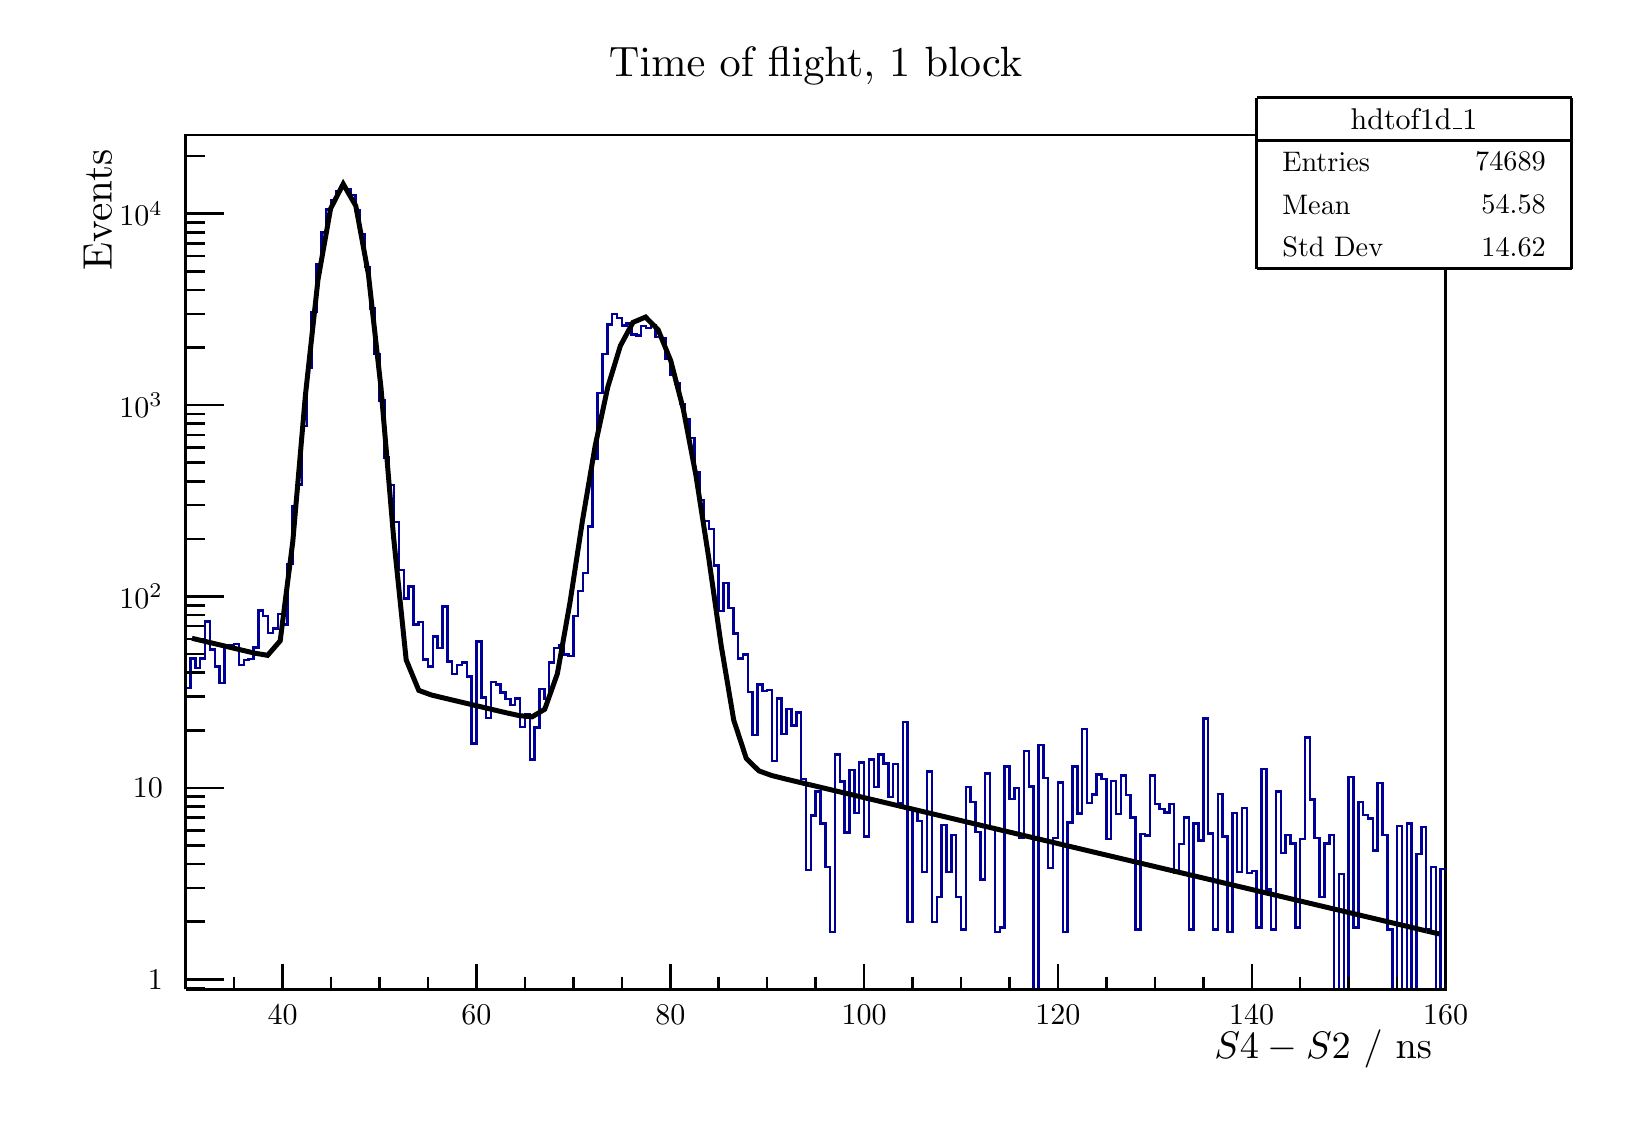
\begin{tikzpicture}
\pgfdeclareplotmark{cross} {
\pgfpathmoveto{\pgfpoint{-0.3\pgfplotmarksize}{\pgfplotmarksize}}
\pgfpathlineto{\pgfpoint{+0.3\pgfplotmarksize}{\pgfplotmarksize}}
\pgfpathlineto{\pgfpoint{+0.3\pgfplotmarksize}{0.3\pgfplotmarksize}}
\pgfpathlineto{\pgfpoint{+1\pgfplotmarksize}{0.3\pgfplotmarksize}}
\pgfpathlineto{\pgfpoint{+1\pgfplotmarksize}{-0.3\pgfplotmarksize}}
\pgfpathlineto{\pgfpoint{+0.3\pgfplotmarksize}{-0.3\pgfplotmarksize}}
\pgfpathlineto{\pgfpoint{+0.3\pgfplotmarksize}{-1.\pgfplotmarksize}}
\pgfpathlineto{\pgfpoint{-0.3\pgfplotmarksize}{-1.\pgfplotmarksize}}
\pgfpathlineto{\pgfpoint{-0.3\pgfplotmarksize}{-0.3\pgfplotmarksize}}
\pgfpathlineto{\pgfpoint{-1.\pgfplotmarksize}{-0.3\pgfplotmarksize}}
\pgfpathlineto{\pgfpoint{-1.\pgfplotmarksize}{0.3\pgfplotmarksize}}
\pgfpathlineto{\pgfpoint{-0.3\pgfplotmarksize}{0.3\pgfplotmarksize}}
\pgfpathclose
\pgfusepathqstroke
}
\pgfdeclareplotmark{cross*} {
\pgfpathmoveto{\pgfpoint{-0.3\pgfplotmarksize}{\pgfplotmarksize}}
\pgfpathlineto{\pgfpoint{+0.3\pgfplotmarksize}{\pgfplotmarksize}}
\pgfpathlineto{\pgfpoint{+0.3\pgfplotmarksize}{0.3\pgfplotmarksize}}
\pgfpathlineto{\pgfpoint{+1\pgfplotmarksize}{0.3\pgfplotmarksize}}
\pgfpathlineto{\pgfpoint{+1\pgfplotmarksize}{-0.3\pgfplotmarksize}}
\pgfpathlineto{\pgfpoint{+0.3\pgfplotmarksize}{-0.3\pgfplotmarksize}}
\pgfpathlineto{\pgfpoint{+0.3\pgfplotmarksize}{-1.\pgfplotmarksize}}
\pgfpathlineto{\pgfpoint{-0.3\pgfplotmarksize}{-1.\pgfplotmarksize}}
\pgfpathlineto{\pgfpoint{-0.3\pgfplotmarksize}{-0.3\pgfplotmarksize}}
\pgfpathlineto{\pgfpoint{-1.\pgfplotmarksize}{-0.3\pgfplotmarksize}}
\pgfpathlineto{\pgfpoint{-1.\pgfplotmarksize}{0.3\pgfplotmarksize}}
\pgfpathlineto{\pgfpoint{-0.3\pgfplotmarksize}{0.3\pgfplotmarksize}}
\pgfpathclose
\pgfusepathqfillstroke
}
\pgfdeclareplotmark{newstar} {
\pgfpathmoveto{\pgfqpoint{0pt}{\pgfplotmarksize}}
\pgfpathlineto{\pgfqpointpolar{44}{0.5\pgfplotmarksize}}
\pgfpathlineto{\pgfqpointpolar{18}{\pgfplotmarksize}}
\pgfpathlineto{\pgfqpointpolar{-20}{0.5\pgfplotmarksize}}
\pgfpathlineto{\pgfqpointpolar{-54}{\pgfplotmarksize}}
\pgfpathlineto{\pgfqpointpolar{-90}{0.5\pgfplotmarksize}}
\pgfpathlineto{\pgfqpointpolar{234}{\pgfplotmarksize}}
\pgfpathlineto{\pgfqpointpolar{198}{0.5\pgfplotmarksize}}
\pgfpathlineto{\pgfqpointpolar{162}{\pgfplotmarksize}}
\pgfpathlineto{\pgfqpointpolar{134}{0.5\pgfplotmarksize}}
\pgfpathclose
\pgfusepathqstroke
}
\pgfdeclareplotmark{newstar*} {
\pgfpathmoveto{\pgfqpoint{0pt}{\pgfplotmarksize}}
\pgfpathlineto{\pgfqpointpolar{44}{0.5\pgfplotmarksize}}
\pgfpathlineto{\pgfqpointpolar{18}{\pgfplotmarksize}}
\pgfpathlineto{\pgfqpointpolar{-20}{0.5\pgfplotmarksize}}
\pgfpathlineto{\pgfqpointpolar{-54}{\pgfplotmarksize}}
\pgfpathlineto{\pgfqpointpolar{-90}{0.5\pgfplotmarksize}}
\pgfpathlineto{\pgfqpointpolar{234}{\pgfplotmarksize}}
\pgfpathlineto{\pgfqpointpolar{198}{0.5\pgfplotmarksize}}
\pgfpathlineto{\pgfqpointpolar{162}{\pgfplotmarksize}}
\pgfpathlineto{\pgfqpointpolar{134}{0.5\pgfplotmarksize}}
\pgfpathclose
\pgfusepathqfillstroke
}
\definecolor{c}{rgb}{1,1,1};
\draw [color=c, fill=c] (0,0) rectangle (20,13.5632);
\draw [color=c, fill=c] (2,1.35632) rectangle (18,12.2069);
\definecolor{c}{rgb}{0,0,0};
\draw [c,line width=0.9] (2,1.35632) -- (2,12.2069) -- (18,12.2069) -- (18,1.35632) -- (2,1.35632);
\definecolor{c}{rgb}{1,1,1};
\draw [color=c, fill=c] (2,1.35632) rectangle (18,12.2069);
\definecolor{c}{rgb}{0,0,0};
\draw [c,line width=0.9] (2,1.35632) -- (2,12.2069) -- (18,12.2069) -- (18,1.35632) -- (2,1.35632);
\definecolor{c}{rgb}{0,0,0.6};
\draw [c,line width=0.9] (2,5.18151) -- (2.06154,5.18151) -- (2.06154,5.55608) -- (2.12308,5.55608) -- (2.12308,5.43961) -- (2.18462,5.43961) -- (2.18462,5.55581) -- (2.24615,5.55581) -- (2.24615,6.03099) -- (2.30769,6.03099) -- (2.30769,5.671) --
 (2.36923,5.671) -- (2.36923,5.45689) -- (2.43077,5.45689) -- (2.43077,5.24567) -- (2.49231,5.24567) -- (2.49231,5.73078) -- (2.55385,5.73078) -- (2.55385,5.72665) -- (2.61538,5.72665) -- (2.61538,5.74226) -- (2.67692,5.74226) -- (2.67692,5.47851) --
 (2.73846,5.47851) -- (2.73846,5.53808) -- (2.8,5.53808) -- (2.8,5.54976) -- (2.86154,5.54976) -- (2.86154,5.69856) -- (2.92308,5.69856) -- (2.92308,6.16999) -- (2.98462,6.16999) -- (2.98462,6.10032) -- (3.04615,6.10032) -- (3.04615,5.88449) --
 (3.10769,5.88449) -- (3.10769,5.93992) -- (3.16923,5.93992) -- (3.16923,6.12156) -- (3.23077,6.12156) -- (3.23077,5.99356) -- (3.29231,5.99356) -- (3.29231,6.75831) -- (3.35385,6.75831) -- (3.35385,7.49725) -- (3.41538,7.49725) -- (3.41538,7.76618)
 -- (3.47692,7.76618) -- (3.47692,8.5123) -- (3.53846,8.5123) -- (3.53846,9.25065) -- (3.6,9.25065) -- (3.6,9.95823) -- (3.66154,9.95823) -- (3.66154,10.5598) -- (3.72308,10.5598) -- (3.72308,10.9657) -- (3.78462,10.9657) -- (3.78462,11.2595) --
 (3.84615,11.2595) -- (3.84615,11.3826) -- (3.90769,11.3826) -- (3.90769,11.4937) -- (3.96923,11.4937) -- (3.96923,11.5322) -- (4.03077,11.5322) -- (4.03077,11.5125) -- (4.09231,11.5125) -- (4.09231,11.4476) -- (4.15385,11.4476) -- (4.15385,11.2503)
 -- (4.21538,11.2503) -- (4.21538,10.9505) -- (4.27692,10.9505) -- (4.27692,10.5305) -- (4.33846,10.5305) -- (4.33846,10.0019) -- (4.4,10.0019) -- (4.4,9.42602) -- (4.46154,9.42602) -- (4.46154,8.83371) -- (4.52308,8.83371) -- (4.52308,8.11005) --
 (4.58462,8.11005) -- (4.58462,7.76378) -- (4.64615,7.76378) -- (4.64615,7.29171) -- (4.70769,7.29171) -- (4.70769,6.67972) -- (4.76923,6.67972) -- (4.76923,6.32169) -- (4.83077,6.32169) -- (4.83077,6.47204) -- (4.89231,6.47204) -- (4.89231,5.993) --
 (4.95385,5.993) -- (4.95385,6.02017) -- (5.01538,6.02017) -- (5.01538,5.54748) -- (5.07692,5.54748) -- (5.07692,5.45714) -- (5.13846,5.45714) -- (5.13846,5.83864) -- (5.2,5.83864) -- (5.2,5.69096) -- (5.26154,5.69096) -- (5.26154,6.21606) --
 (5.32308,6.21606) -- (5.32308,5.51754) -- (5.38462,5.51754) -- (5.38462,5.35984) -- (5.44615,5.35984) -- (5.44615,5.47524) -- (5.50769,5.47524) -- (5.50769,5.50812) -- (5.56923,5.50812) -- (5.56923,5.32886) -- (5.63077,5.32886) -- (5.63077,4.47719)
 -- (5.69231,4.47719) -- (5.69231,5.77627) -- (5.75385,5.77627) -- (5.75385,5.06195) -- (5.81538,5.06195) -- (5.81538,4.80233) -- (5.87692,4.80233) -- (5.87692,5.25956) -- (5.93846,5.25956) -- (5.93846,5.22936) -- (6,5.22936) -- (6,5.12667) --
 (6.06154,5.12667) -- (6.06154,5.04604) -- (6.12308,5.04604) -- (6.12308,4.96718) -- (6.18462,4.96718) -- (6.18462,5.05252) -- (6.24615,5.05252) -- (6.24615,4.68623) -- (6.30769,4.68623) -- (6.30769,4.85157) -- (6.36923,4.85157) -- (6.36923,4.2741)
 -- (6.43077,4.2741) -- (6.43077,4.68523) -- (6.49231,4.68523) -- (6.49231,5.16964) -- (6.55385,5.16964) -- (6.55385,5.0443) -- (6.61538,5.0443) -- (6.61538,5.50863) -- (6.67692,5.50863) -- (6.67692,5.68975) -- (6.73846,5.68975) -- (6.73846,5.72166)
 -- (6.8,5.72166) -- (6.8,5.60763) -- (6.86154,5.60763) -- (6.86154,5.58722) -- (6.92308,5.58722) -- (6.92308,6.09935) -- (6.98462,6.09935) -- (6.98462,6.41753) -- (7.04615,6.41753) -- (7.04615,6.64659) -- (7.10769,6.64659) -- (7.10769,7.2355) --
 (7.16923,7.2355) -- (7.16923,8.09892) -- (7.23077,8.09892) -- (7.23077,8.93136) -- (7.29231,8.93136) -- (7.29231,9.42351) -- (7.35385,9.42351) -- (7.35385,9.79794) -- (7.41538,9.79794) -- (7.41538,9.93183) -- (7.47692,9.93183) -- (7.47692,9.8799) --
 (7.53846,9.8799) -- (7.53846,9.78722) -- (7.6,9.78722) -- (7.6,9.81608) -- (7.66154,9.81608) -- (7.66154,9.67331) -- (7.72308,9.67331) -- (7.72308,9.65902) -- (7.78462,9.65902) -- (7.78462,9.77948) -- (7.84615,9.77948) -- (7.84615,9.75876) --
 (7.90769,9.75876) -- (7.90769,9.79026) -- (7.96923,9.79026) -- (7.96923,9.64053) -- (8.03077,9.64053) -- (8.03077,9.63187) -- (8.09231,9.63187) -- (8.09231,9.36831) -- (8.15385,9.36831) -- (8.15385,9.16368) -- (8.21538,9.16368) -- (8.21538,9.05403)
 -- (8.27692,9.05403) -- (8.27692,8.78876) -- (8.33846,8.78876) -- (8.33846,8.603) -- (8.4,8.603) -- (8.4,8.35968) -- (8.46154,8.35968) -- (8.46154,7.91883) -- (8.52308,7.91883) -- (8.52308,7.56846) -- (8.58462,7.56846) -- (8.58462,7.30407) --
 (8.64615,7.30407) -- (8.64615,7.20532) -- (8.70769,7.20532) -- (8.70769,6.74177) -- (8.76923,6.74177) -- (8.76923,6.16352) -- (8.83077,6.16352) -- (8.83077,6.51821) -- (8.89231,6.51821) -- (8.89231,6.20221) -- (8.95385,6.20221) -- (8.95385,5.87638)
 -- (9.01538,5.87638) -- (9.01538,5.55625) -- (9.07692,5.55625) -- (9.07692,5.61066) -- (9.13846,5.61066) -- (9.13846,5.13328) -- (9.2,5.13328) -- (9.2,4.58783) -- (9.26154,4.58783) -- (9.26154,5.23012) -- (9.32308,5.23012) -- (9.32308,5.146) --
 (9.38461,5.146) -- (9.38461,5.15776) -- (9.44615,5.15776) -- (9.44615,4.25767) -- (9.50769,4.25767) -- (9.50769,5.04774) -- (9.56923,5.04774) -- (9.56923,4.60175) -- (9.63077,4.60175) -- (9.63077,4.92009) -- (9.69231,4.92009) -- (9.69231,4.71042) --
 (9.75385,4.71042) -- (9.75385,4.87061) -- (9.81538,4.87061) -- (9.81538,4.02592) -- (9.87692,4.02592) -- (9.87692,2.87449) -- (9.93846,2.87449) -- (9.93846,3.56693) -- (10,3.56693) -- (10,3.87246) -- (10.0615,3.87246) -- (10.0615,3.4613) --
 (10.1231,3.4613) -- (10.1231,2.90853) -- (10.1846,2.90853) -- (10.1846,2.08809) -- (10.2462,2.08809) -- (10.2462,4.33668) -- (10.3077,4.33668) -- (10.3077,3.99697) -- (10.3692,3.99697) -- (10.3692,3.3477) -- (10.4308,3.3477) -- (10.4308,4.13973) --
 (10.4923,4.13973) -- (10.4923,3.59781) -- (10.5538,3.59781) -- (10.5538,4.23774) -- (10.6154,4.23774) -- (10.6154,3.29987) -- (10.6769,3.29987) -- (10.6769,4.27622) -- (10.7385,4.27622) -- (10.7385,3.92545) -- (10.8,3.92545) -- (10.8,4.34213) --
 (10.8615,4.34213) -- (10.8615,4.22691) -- (10.9231,4.22691) -- (10.9231,3.79686) -- (10.9846,3.79686) -- (10.9846,4.22057) -- (11.0462,4.22057) -- (11.0462,3.71905) -- (11.1077,3.71905) -- (11.1077,4.75094) -- (11.1692,4.75094) -- (11.1692,2.20974)
 -- (11.2308,2.20974) -- (11.2308,3.65017) -- (11.2923,3.65017) -- (11.2923,3.492) -- (11.3538,3.492) -- (11.3538,2.84753) -- (11.4154,2.84753) -- (11.4154,4.12337) -- (11.4769,4.12337) -- (11.4769,2.20974) -- (11.5385,2.20974) -- (11.5385,2.53059)
 -- (11.6,2.53059) -- (11.6,3.44296) -- (11.6615,3.44296) -- (11.6615,2.84753) -- (11.7231,2.84753) -- (11.7231,3.31942) -- (11.7846,3.31942) -- (11.7846,2.53059) -- (11.8462,2.53059) -- (11.8462,2.11846) -- (11.9077,2.11846) -- (11.9077,3.92545) --
 (11.9692,3.92545) -- (11.9692,3.73625) -- (12.0308,3.73625) -- (12.0308,3.35377) -- (12.0923,3.35377) -- (12.0923,2.74928) -- (12.1538,2.74928) -- (12.1538,4.09554) -- (12.2154,4.09554) -- (12.2154,3.41687) -- (12.2769,3.41687) -- (12.2769,2.08809)
 -- (12.3385,2.08809) -- (12.3385,2.14272) -- (12.4,2.14272) -- (12.4,4.18641) -- (12.4615,4.18641) -- (12.4615,3.77723) -- (12.5231,3.77723) -- (12.5231,3.91398) -- (12.5846,3.91398) -- (12.5846,3.27829) -- (12.6462,3.27829) -- (12.6462,4.38363) --
 (12.7077,4.38363) -- (12.7077,3.93124) -- (12.7692,3.93124) -- (12.7692,1.35632) -- (12.8308,1.35632) -- (12.8308,4.45728) -- (12.8923,4.45728) -- (12.8923,4.04146) -- (12.9538,4.04146) -- (12.9538,2.89686) -- (13.0154,2.89686) -- (13.0154,3.27649)
 -- (13.0769,3.27649) -- (13.0769,3.98168) -- (13.1385,3.98168) -- (13.1385,2.08809) -- (13.2,2.08809) -- (13.2,3.47404) -- (13.2615,3.47404) -- (13.2615,4.18641) -- (13.3231,4.18641) -- (13.3231,3.58812) -- (13.3846,3.58812) -- (13.3846,4.66074) --
 (13.4462,4.66074) -- (13.4462,3.72096) -- (13.5077,3.72096) -- (13.5077,3.83058) -- (13.5692,3.83058) -- (13.5692,4.08766) -- (13.6308,4.08766) -- (13.6308,4.03023) -- (13.6923,4.03023) -- (13.6923,3.26645) -- (13.7538,3.26645) -- (13.7538,4.00415)
 -- (13.8154,4.00415) -- (13.8154,3.58678) -- (13.8769,3.58678) -- (13.8769,4.07563) -- (13.9385,4.07563) -- (13.9385,3.82377) -- (14,3.82377) -- (14,3.53914) -- (14.0615,3.53914) -- (14.0615,2.11846) -- (14.1231,2.11846) -- (14.1231,3.33056) --
 (14.1846,3.33056) -- (14.1846,3.3096) -- (14.2462,3.3096) -- (14.2462,4.07579) -- (14.3077,4.07579) -- (14.3077,3.70785) -- (14.3692,3.70785) -- (14.3692,3.64917) -- (14.4308,3.64917) -- (14.4308,3.60516) -- (14.4923,3.60516) -- (14.4923,3.70785) --
 (14.5538,3.70785) -- (14.5538,2.83516) -- (14.6154,2.83516) -- (14.6154,3.20139) -- (14.6769,3.20139) -- (14.6769,3.53914) -- (14.7385,3.53914) -- (14.7385,2.11846) -- (14.8,2.11846) -- (14.8,3.46572) -- (14.8615,3.46572) -- (14.8615,3.24538) --
 (14.9231,3.24538) -- (14.9231,4.79484) -- (14.9846,4.79484) -- (14.9846,3.33729) -- (15.0462,3.33729) -- (15.0462,2.11846) -- (15.1077,2.11846) -- (15.1077,3.83614) -- (15.1692,3.83614) -- (15.1692,3.29647) -- (15.2308,3.29647) -- (15.2308,2.08809)
 -- (15.2923,2.08809) -- (15.2923,3.59713) -- (15.3538,3.59713) -- (15.3538,2.85023) -- (15.4154,2.85023) -- (15.4154,3.66286) -- (15.4769,3.66286) -- (15.4769,2.83516) -- (15.5385,2.83516) -- (15.5385,2.86243) -- (15.6,2.86243) -- (15.6,2.14272) --
 (15.6615,2.14272) -- (15.6615,4.15383) -- (15.7231,4.15383) -- (15.7231,2.62199) -- (15.7846,2.62199) -- (15.7846,2.11846) -- (15.8462,2.11846) -- (15.8462,3.87165) -- (15.9077,3.87165) -- (15.9077,3.08614) -- (15.9692,3.08614) -- (15.9692,3.31751)
 -- (16.0308,3.31751) -- (16.0308,3.21207) -- (16.0923,3.21207) -- (16.0923,2.14272) -- (16.1538,2.14272) -- (16.1538,3.26826) -- (16.2154,3.26826) -- (16.2154,4.55325) -- (16.2769,4.55325) -- (16.2769,3.77087) -- (16.3385,3.77087) --
 (16.3385,3.27829) -- (16.4,3.27829) -- (16.4,2.53059) -- (16.4615,2.53059) -- (16.4615,3.21207) -- (16.5231,3.21207) -- (16.5231,3.31751) -- (16.5846,3.31751) -- (16.5846,1.35632) -- (16.6462,1.35632) -- (16.6462,2.81986) -- (16.7077,2.81986) --
 (16.7077,1.35632) -- (16.7692,1.35632) -- (16.7692,4.05445) -- (16.8308,4.05445) -- (16.8308,2.14272) -- (16.8923,2.14272) -- (16.8923,3.7376) -- (16.9538,3.7376) -- (16.9538,3.57313) -- (17.0154,3.57313) -- (17.0154,3.52486) -- (17.0769,3.52486) --
 (17.0769,3.12021) -- (17.1385,3.12021) -- (17.1385,3.98035) -- (17.2,3.98035) -- (17.2,3.31751) -- (17.2615,3.31751) -- (17.2615,2.11846) -- (17.3231,2.11846) -- (17.3231,1.35632) -- (17.3846,1.35632) -- (17.3846,3.43423) -- (17.4462,3.43423) --
 (17.4462,1.35632) -- (17.5077,1.35632) -- (17.5077,3.4613) -- (17.5692,3.4613) -- (17.5692,1.35632) -- (17.6308,1.35632) -- (17.6308,3.07628) -- (17.6923,3.07628) -- (17.6923,3.41932) -- (17.7538,3.41932) -- (17.7538,2.11846) -- (17.8154,2.11846) --
 (17.8154,2.90853) -- (17.8769,2.90853) -- (17.8769,1.35632) -- (17.9385,1.35632) -- (17.9385,2.88244) -- (18,2.88244);
\definecolor{c}{rgb}{0,0,0};
\draw [c,line width=0.9] (2,1.35632) -- (18,1.35632);
\draw [anchor= east] (18,0.596782) node[scale=1.38496, color=c, rotate=0]{$S4 - S2$ / ns};
\draw [c,line width=0.9] (3.23077,1.68184) -- (3.23077,1.35632);
\draw [c,line width=0.9] (3.84615,1.51908) -- (3.84615,1.35632);
\draw [c,line width=0.9] (4.46154,1.51908) -- (4.46154,1.35632);
\draw [c,line width=0.9] (5.07692,1.51908) -- (5.07692,1.35632);
\draw [c,line width=0.9] (5.69231,1.68184) -- (5.69231,1.35632);
\draw [c,line width=0.9] (6.30769,1.51908) -- (6.30769,1.35632);
\draw [c,line width=0.9] (6.92308,1.51908) -- (6.92308,1.35632);
\draw [c,line width=0.9] (7.53846,1.51908) -- (7.53846,1.35632);
\draw [c,line width=0.9] (8.15385,1.68184) -- (8.15385,1.35632);
\draw [c,line width=0.9] (8.76923,1.51908) -- (8.76923,1.35632);
\draw [c,line width=0.9] (9.38461,1.51908) -- (9.38461,1.35632);
\draw [c,line width=0.9] (10,1.51908) -- (10,1.35632);
\draw [c,line width=0.9] (10.6154,1.68184) -- (10.6154,1.35632);
\draw [c,line width=0.9] (11.2308,1.51908) -- (11.2308,1.35632);
\draw [c,line width=0.9] (11.8462,1.51908) -- (11.8462,1.35632);
\draw [c,line width=0.9] (12.4615,1.51908) -- (12.4615,1.35632);
\draw [c,line width=0.9] (13.0769,1.68184) -- (13.0769,1.35632);
\draw [c,line width=0.9] (13.6923,1.51908) -- (13.6923,1.35632);
\draw [c,line width=0.9] (14.3077,1.51908) -- (14.3077,1.35632);
\draw [c,line width=0.9] (14.9231,1.51908) -- (14.9231,1.35632);
\draw [c,line width=0.9] (15.5385,1.68184) -- (15.5385,1.35632);
\draw [c,line width=0.9] (16.1538,1.51908) -- (16.1538,1.35632);
\draw [c,line width=0.9] (16.7692,1.51908) -- (16.7692,1.35632);
\draw [c,line width=0.9] (17.3846,1.51908) -- (17.3846,1.35632);
\draw [c,line width=0.9] (18,1.68184) -- (18,1.35632);
\draw [c,line width=0.9] (3.23077,1.68184) -- (3.23077,1.35632);
\draw [c,line width=0.9] (2.61538,1.51908) -- (2.61538,1.35632);
\draw [c,line width=0.9] (2,1.51908) -- (2,1.35632);
\draw [anchor=base] (3.23077,0.908736) node[scale=1.08496, color=c, rotate=0]{40};
\draw [anchor=base] (5.69231,0.908736) node[scale=1.08496, color=c, rotate=0]{60};
\draw [anchor=base] (8.15385,0.908736) node[scale=1.08496, color=c, rotate=0]{80};
\draw [anchor=base] (10.6154,0.908736) node[scale=1.08496, color=c, rotate=0]{100};
\draw [anchor=base] (13.0769,0.908736) node[scale=1.08496, color=c, rotate=0]{120};
\draw [anchor=base] (15.5385,0.908736) node[scale=1.08496, color=c, rotate=0]{140};
\draw [anchor=base] (18,0.908736) node[scale=1.08496, color=c, rotate=0]{160};
\draw [c,line width=0.9] (2,1.35632) -- (2,12.2069);
\draw [anchor= east] (0.88,12.2069) node[scale=1.48496, color=c, rotate=90]{ Events};
\draw [c,line width=0.9] (2.24,1.37274) -- (2,1.37274);
\draw [c,line width=0.9] (2.48,1.48397) -- (2,1.48397);
\draw [anchor= east] (1.844,1.48397) node[scale=1.08496, color=c, rotate=0]{1};
\draw [c,line width=0.9] (2.24,2.21574) -- (2,2.21574);
\draw [c,line width=0.9] (2.24,2.6438) -- (2,2.6438);
\draw [c,line width=0.9] (2.24,2.94751) -- (2,2.94751);
\draw [c,line width=0.9] (2.24,3.18309) -- (2,3.18309);
\draw [c,line width=0.9] (2.24,3.37557) -- (2,3.37557);
\draw [c,line width=0.9] (2.24,3.53831) -- (2,3.53831);
\draw [c,line width=0.9] (2.24,3.67928) -- (2,3.67928);
\draw [c,line width=0.9] (2.24,3.80363) -- (2,3.80363);
\draw [c,line width=0.9] (2.48,3.91486) -- (2,3.91486);
\draw [anchor= east] (1.844,3.91486) node[scale=1.08496, color=c, rotate=0]{10};
\draw [c,line width=0.9] (2.24,4.64663) -- (2,4.64663);
\draw [c,line width=0.9] (2.24,5.07469) -- (2,5.07469);
\draw [c,line width=0.9] (2.24,5.3784) -- (2,5.3784);
\draw [c,line width=0.9] (2.24,5.61398) -- (2,5.61398);
\draw [c,line width=0.9] (2.24,5.80646) -- (2,5.80646);
\draw [c,line width=0.9] (2.24,5.9692) -- (2,5.9692);
\draw [c,line width=0.9] (2.24,6.11017) -- (2,6.11017);
\draw [c,line width=0.9] (2.24,6.23452) -- (2,6.23452);
\draw [c,line width=0.9] (2.48,6.34575) -- (2,6.34575);
\draw [anchor= east] (1.844,6.34575) node[scale=1.08496, color=c, rotate=0]{$10^{2}$};
\draw [c,line width=0.9] (2.24,7.07752) -- (2,7.07752);
\draw [c,line width=0.9] (2.24,7.50558) -- (2,7.50558);
\draw [c,line width=0.9] (2.24,7.80929) -- (2,7.80929);
\draw [c,line width=0.9] (2.24,8.04487) -- (2,8.04487);
\draw [c,line width=0.9] (2.24,8.23735) -- (2,8.23735);
\draw [c,line width=0.9] (2.24,8.40009) -- (2,8.40009);
\draw [c,line width=0.9] (2.24,8.54106) -- (2,8.54106);
\draw [c,line width=0.9] (2.24,8.66541) -- (2,8.66541);
\draw [c,line width=0.9] (2.48,8.77664) -- (2,8.77664);
\draw [anchor= east] (1.844,8.77664) node[scale=1.08496, color=c, rotate=0]{$10^{3}$};
\draw [c,line width=0.9] (2.24,9.50841) -- (2,9.50841);
\draw [c,line width=0.9] (2.24,9.93647) -- (2,9.93647);
\draw [c,line width=0.9] (2.24,10.2402) -- (2,10.2402);
\draw [c,line width=0.9] (2.24,10.4758) -- (2,10.4758);
\draw [c,line width=0.9] (2.24,10.6682) -- (2,10.6682);
\draw [c,line width=0.9] (2.24,10.831) -- (2,10.831);
\draw [c,line width=0.9] (2.24,10.9719) -- (2,10.9719);
\draw [c,line width=0.9] (2.24,11.0963) -- (2,11.0963);
\draw [c,line width=0.9] (2.48,11.2075) -- (2,11.2075);
\draw [anchor= east] (1.844,11.2075) node[scale=1.08496, color=c, rotate=0]{$10^{4}$};
\draw [c,line width=0.9] (2.24,11.9393) -- (2,11.9393);
\definecolor{c}{rgb}{1,1,1};
\draw [color=c, fill=c] (15.6,10.5115) rectangle (19.6,12.6816);
\definecolor{c}{rgb}{0,0,0};
\draw [c,line width=0.9] (15.6,10.5115) -- (19.6,10.5115);
\draw [c,line width=0.9] (19.6,10.5115) -- (19.6,12.6816);
\draw [c,line width=0.9] (19.6,12.6816) -- (15.6,12.6816);
\draw [c,line width=0.9] (15.6,12.6816) -- (15.6,10.5115);
\draw (17.6,12.4103) node[scale=1.08496, color=c, rotate=0]{hdtof1d\_1};
\draw [c,line width=0.9] (15.6,12.1391) -- (19.6,12.1391);
\draw [anchor= west] (15.8,11.8678) node[scale=1.02114, color=c, rotate=0]{Entries };
\draw [anchor= east] (19.4,11.8678) node[scale=1.02114, color=c, rotate=0]{ 74689};
\draw [anchor= west] (15.8,11.3253) node[scale=1.02114, color=c, rotate=0]{Mean  };
\draw [anchor= east] (19.4,11.3253) node[scale=1.02114, color=c, rotate=0]{  54.58};
\draw [anchor= west] (15.8,10.7828) node[scale=1.02114, color=c, rotate=0]{Std Dev   };
\draw [anchor= east] (19.4,10.7828) node[scale=1.02114, color=c, rotate=0]{  14.62};
\draw [c,line width=1.8] (2.08,5.81522) -- (2.24,5.77729) -- (2.4,5.73936) -- (2.56,5.70143) -- (2.72,5.6635) -- (2.88,5.62584) -- (3.04,5.59883) -- (3.2,5.783) -- (3.36,7.04462) -- (3.52,8.89992) -- (3.68,10.3694) -- (3.84,11.2716) -- (4,11.5852) --
 (4.16,11.3072) -- (4.32,10.4394) -- (4.48,8.9965) -- (4.64,7.0994) -- (4.8,5.54055) -- (4.96,5.1535) -- (5.12,5.09513) -- (5.28,5.05662) -- (5.44,5.01869) -- (5.6,4.98076) -- (5.76,4.94283) -- (5.92,4.90492) -- (6.08,4.86731) -- (6.24,4.83246) --
 (6.4,4.81808) -- (6.56,4.91497) -- (6.72,5.3653) -- (6.88,6.26787) -- (7.04,7.31709) -- (7.2,8.25867) -- (7.36,9.00435) -- (7.52,9.52953) -- (7.68,9.82711) -- (7.84,9.89492) -- (8,9.73249) -- (8.16,9.34039) -- (8.32,8.721) -- (8.48,7.88215) --
 (8.64,6.85117) -- (8.8,5.72561) -- (8.96,4.77556) -- (9.12,4.2879) -- (9.28,4.13137) -- (9.44,4.0733) -- (9.6,4.03279) -- (9.76,3.9946) -- (9.92,3.95665);
\draw [c,line width=1.8] (9.92,3.95665) -- (10.08,3.91871) -- (10.24,3.88078) -- (10.4,3.84285) -- (10.56,3.80492) -- (10.72,3.76699) -- (10.88,3.72906) -- (11.04,3.69113) -- (11.2,3.6532) -- (11.36,3.61527) -- (11.52,3.57734) -- (11.68,3.53941) --
 (11.84,3.50148) -- (12,3.46355) -- (12.16,3.42562) -- (12.32,3.38769) -- (12.48,3.34976) -- (12.64,3.31183) -- (12.8,3.2739) -- (12.96,3.23597) -- (13.12,3.19804) -- (13.28,3.16011) -- (13.44,3.12218) -- (13.6,3.08425) -- (13.76,3.04632) --
 (13.92,3.00839) -- (14.08,2.97046) -- (14.24,2.93253) -- (14.4,2.8946) -- (14.56,2.85667) -- (14.72,2.81874) -- (14.88,2.78081) -- (15.04,2.74288) -- (15.2,2.70495) -- (15.36,2.66702) -- (15.52,2.62909) -- (15.68,2.59116) -- (15.84,2.55323) --
 (16,2.5153) -- (16.16,2.47737) -- (16.32,2.43944) -- (16.48,2.40151) -- (16.64,2.36358) -- (16.8,2.32565) -- (16.96,2.28772) -- (17.12,2.24979) -- (17.28,2.21186) -- (17.44,2.17393) -- (17.6,2.136) -- (17.76,2.09807);
\draw [c,line width=1.8] (17.76,2.09807) -- (17.92,2.06014);
\draw (10,13.0816) node[scale=1.5317, color=c, rotate=0]{Time of flight, 1 block};
\end{tikzpicture}

		\end{adjustbox}
		\caption{Example of the time of flight spectrum observed in $S4$ with a combined signal and background function fitted (shown in black)}
		\label{fig:fitEx}
	\end{figure}

	To produce the data used in this analysis, an exponential background function is subtracted. 
	The parameters for this function are taken from the combined signal and background function.

	Figure~\ref{fig:s3tof} shows the time of flight spectrum recorded in the $S3$ timing point for varying numbers of moderator blocks.
	Similarly to figure~\ref{fig:s4tof}, the quicker peak is formed by minimum ionizing particles, while the peak at higher values of $S3 - S1$ corresponds to protons.
	\begin{figure}[h]
		\begin{adjustbox}{max totalsize={.8\textwidth}{.5\textheight},center}
			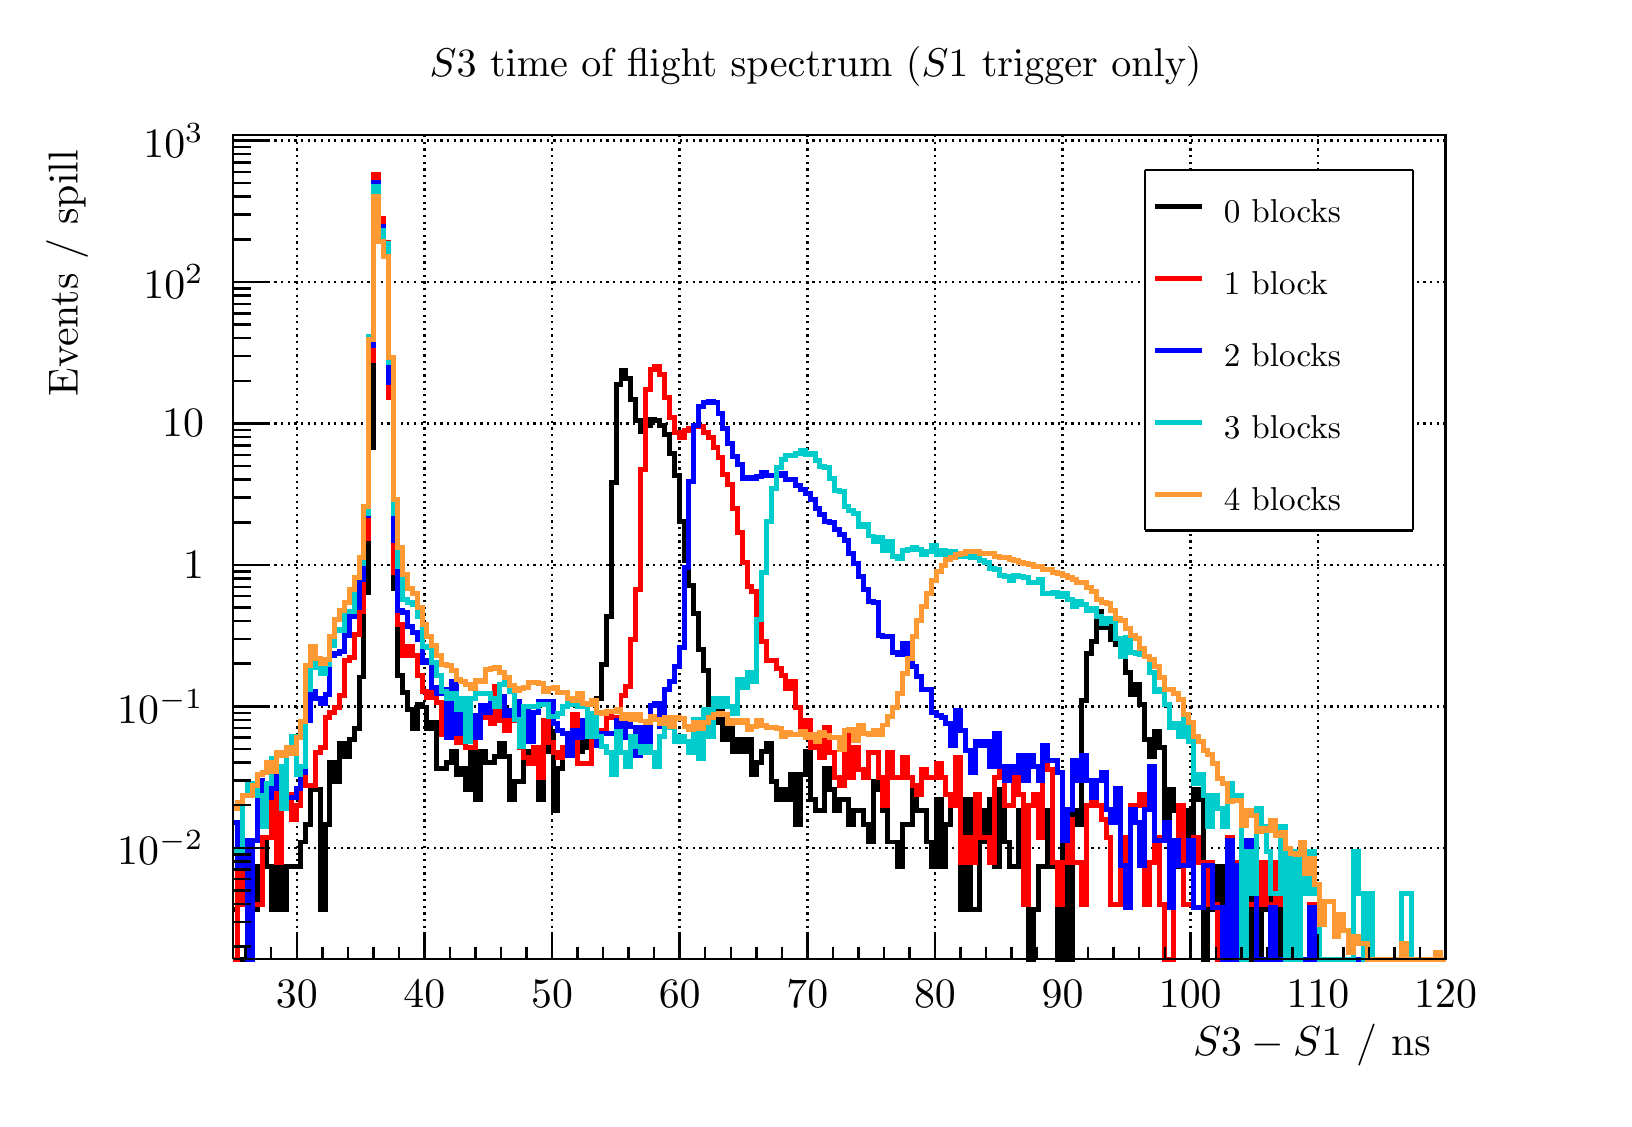
\begin{tikzpicture}
\pgfdeclareplotmark{cross} {
\pgfpathmoveto{\pgfpoint{-0.3\pgfplotmarksize}{\pgfplotmarksize}}
\pgfpathlineto{\pgfpoint{+0.3\pgfplotmarksize}{\pgfplotmarksize}}
\pgfpathlineto{\pgfpoint{+0.3\pgfplotmarksize}{0.3\pgfplotmarksize}}
\pgfpathlineto{\pgfpoint{+1\pgfplotmarksize}{0.3\pgfplotmarksize}}
\pgfpathlineto{\pgfpoint{+1\pgfplotmarksize}{-0.3\pgfplotmarksize}}
\pgfpathlineto{\pgfpoint{+0.3\pgfplotmarksize}{-0.3\pgfplotmarksize}}
\pgfpathlineto{\pgfpoint{+0.3\pgfplotmarksize}{-1.\pgfplotmarksize}}
\pgfpathlineto{\pgfpoint{-0.3\pgfplotmarksize}{-1.\pgfplotmarksize}}
\pgfpathlineto{\pgfpoint{-0.3\pgfplotmarksize}{-0.3\pgfplotmarksize}}
\pgfpathlineto{\pgfpoint{-1.\pgfplotmarksize}{-0.3\pgfplotmarksize}}
\pgfpathlineto{\pgfpoint{-1.\pgfplotmarksize}{0.3\pgfplotmarksize}}
\pgfpathlineto{\pgfpoint{-0.3\pgfplotmarksize}{0.3\pgfplotmarksize}}
\pgfpathclose
\pgfusepathqstroke
}
\pgfdeclareplotmark{cross*} {
\pgfpathmoveto{\pgfpoint{-0.3\pgfplotmarksize}{\pgfplotmarksize}}
\pgfpathlineto{\pgfpoint{+0.3\pgfplotmarksize}{\pgfplotmarksize}}
\pgfpathlineto{\pgfpoint{+0.3\pgfplotmarksize}{0.3\pgfplotmarksize}}
\pgfpathlineto{\pgfpoint{+1\pgfplotmarksize}{0.3\pgfplotmarksize}}
\pgfpathlineto{\pgfpoint{+1\pgfplotmarksize}{-0.3\pgfplotmarksize}}
\pgfpathlineto{\pgfpoint{+0.3\pgfplotmarksize}{-0.3\pgfplotmarksize}}
\pgfpathlineto{\pgfpoint{+0.3\pgfplotmarksize}{-1.\pgfplotmarksize}}
\pgfpathlineto{\pgfpoint{-0.3\pgfplotmarksize}{-1.\pgfplotmarksize}}
\pgfpathlineto{\pgfpoint{-0.3\pgfplotmarksize}{-0.3\pgfplotmarksize}}
\pgfpathlineto{\pgfpoint{-1.\pgfplotmarksize}{-0.3\pgfplotmarksize}}
\pgfpathlineto{\pgfpoint{-1.\pgfplotmarksize}{0.3\pgfplotmarksize}}
\pgfpathlineto{\pgfpoint{-0.3\pgfplotmarksize}{0.3\pgfplotmarksize}}
\pgfpathclose
\pgfusepathqfillstroke
}
\pgfdeclareplotmark{newstar} {
\pgfpathmoveto{\pgfqpoint{0pt}{\pgfplotmarksize}}
\pgfpathlineto{\pgfqpointpolar{44}{0.5\pgfplotmarksize}}
\pgfpathlineto{\pgfqpointpolar{18}{\pgfplotmarksize}}
\pgfpathlineto{\pgfqpointpolar{-20}{0.5\pgfplotmarksize}}
\pgfpathlineto{\pgfqpointpolar{-54}{\pgfplotmarksize}}
\pgfpathlineto{\pgfqpointpolar{-90}{0.5\pgfplotmarksize}}
\pgfpathlineto{\pgfqpointpolar{234}{\pgfplotmarksize}}
\pgfpathlineto{\pgfqpointpolar{198}{0.5\pgfplotmarksize}}
\pgfpathlineto{\pgfqpointpolar{162}{\pgfplotmarksize}}
\pgfpathlineto{\pgfqpointpolar{134}{0.5\pgfplotmarksize}}
\pgfpathclose
\pgfusepathqstroke
}
\pgfdeclareplotmark{newstar*} {
\pgfpathmoveto{\pgfqpoint{0pt}{\pgfplotmarksize}}
\pgfpathlineto{\pgfqpointpolar{44}{0.5\pgfplotmarksize}}
\pgfpathlineto{\pgfqpointpolar{18}{\pgfplotmarksize}}
\pgfpathlineto{\pgfqpointpolar{-20}{0.5\pgfplotmarksize}}
\pgfpathlineto{\pgfqpointpolar{-54}{\pgfplotmarksize}}
\pgfpathlineto{\pgfqpointpolar{-90}{0.5\pgfplotmarksize}}
\pgfpathlineto{\pgfqpointpolar{234}{\pgfplotmarksize}}
\pgfpathlineto{\pgfqpointpolar{198}{0.5\pgfplotmarksize}}
\pgfpathlineto{\pgfqpointpolar{162}{\pgfplotmarksize}}
\pgfpathlineto{\pgfqpointpolar{134}{0.5\pgfplotmarksize}}
\pgfpathclose
\pgfusepathqfillstroke
}
\definecolor{c}{rgb}{1,1,1};
\draw [color=c, fill=c] (0,0) rectangle (20,13.5887);
\draw [color=c, fill=c] (2.6,1.76652) rectangle (18,12.2298);
\definecolor{c}{rgb}{0,0,0};
\draw [c,line width=0.9] (2.6,1.76652) -- (2.6,12.2298) -- (18,12.2298) -- (18,1.76652) -- (2.6,1.76652);
\definecolor{c}{rgb}{1,1,1};
\draw [color=c, fill=c] (2.6,1.76652) rectangle (18,12.2298);
\definecolor{c}{rgb}{0,0,0};
\draw [c,line width=0.9] (2.6,1.76652) -- (2.6,12.2298) -- (18,12.2298) -- (18,1.76652) -- (2.6,1.76652);
\draw [c,line width=0.9] (2.6,1.76652) -- (18,1.76652);
\draw [c,dash pattern=on 0.80pt off 1.60pt ,line width=0.9] (3.41053,12.2298) -- (3.41053,1.76652);
\draw [c,dash pattern=on 0.80pt off 1.60pt ,line width=0.9] (5.03158,12.2298) -- (5.03158,1.76652);
\draw [c,dash pattern=on 0.80pt off 1.60pt ,line width=0.9] (6.65263,12.2298) -- (6.65263,1.76652);
\draw [c,dash pattern=on 0.80pt off 1.60pt ,line width=0.9] (8.27368,12.2298) -- (8.27368,1.76652);
\draw [c,dash pattern=on 0.80pt off 1.60pt ,line width=0.9] (9.89474,12.2298) -- (9.89474,1.76652);
\draw [c,dash pattern=on 0.80pt off 1.60pt ,line width=0.9] (11.5158,12.2298) -- (11.5158,1.76652);
\draw [c,dash pattern=on 0.80pt off 1.60pt ,line width=0.9] (13.1368,12.2298) -- (13.1368,1.76652);
\draw [c,dash pattern=on 0.80pt off 1.60pt ,line width=0.9] (14.7579,12.2298) -- (14.7579,1.76652);
\draw [c,dash pattern=on 0.80pt off 1.60pt ,line width=0.9] (16.3789,12.2298) -- (16.3789,1.76652);
\draw [c,dash pattern=on 0.80pt off 1.60pt ,line width=0.9] (18,12.2298) -- (18,1.76652);
\draw [c,dash pattern=on 0.80pt off 1.60pt ,line width=0.9] (3.41053,12.2298) -- (3.41053,1.76652);
\draw [c,line width=0.9] (2.6,1.76652) -- (2.6,12.2298);
\draw [c,dash pattern=on 0.80pt off 1.60pt ,line width=0.9] (18,3.1801) -- (2.6,3.1801);
\draw [c,dash pattern=on 0.80pt off 1.60pt ,line width=0.9] (18,4.97682) -- (2.6,4.97682);
\draw [c,dash pattern=on 0.80pt off 1.60pt ,line width=0.9] (18,6.77354) -- (2.6,6.77354);
\draw [c,dash pattern=on 0.80pt off 1.60pt ,line width=0.9] (18,8.57026) -- (2.6,8.57026);
\draw [c,dash pattern=on 0.80pt off 1.60pt ,line width=0.9] (18,10.367) -- (2.6,10.367);
\draw [c,dash pattern=on 0.80pt off 1.60pt ,line width=0.9] (18,12.1637) -- (2.6,12.1637);
\definecolor{c}{rgb}{0,0,0.6};
\draw [c,line width=0.9] (2.6,1.76652) -- (2.6616,1.76652) -- (2.6616,1.76652) -- (2.7232,1.76652) -- (2.7232,1.76652) -- (2.7848,1.76652) -- (2.7848,1.76652) -- (2.8464,1.76652) -- (2.8464,1.76652) -- (2.908,1.76652) -- (2.908,1.76652) --
 (2.9696,1.76652) -- (2.9696,1.76652) -- (3.0312,1.76652) -- (3.0312,1.76652) -- (3.0928,1.76652) -- (3.0928,1.76652) -- (3.1544,1.76652) -- (3.1544,1.76652) -- (3.216,1.76652) -- (3.216,1.76652) -- (3.2776,1.76652) -- (3.2776,1.76652) --
 (3.3392,1.76652) -- (3.3392,1.76652) -- (3.4008,1.76652) -- (3.4008,1.76652) -- (3.4624,1.76652) -- (3.4624,1.76652) -- (3.524,1.76652) -- (3.524,1.76652) -- (3.5856,1.76652) -- (3.5856,1.76652) -- (3.6472,1.76652) -- (3.6472,1.76652) --
 (3.7088,1.76652) -- (3.7088,1.76652) -- (3.7704,1.76652) -- (3.7704,1.76652) -- (3.832,1.76652) -- (3.832,1.76652) -- (3.8936,1.76652) -- (3.8936,1.76652) -- (3.9552,1.76652) -- (3.9552,1.76652) -- (4.0168,1.76652) -- (4.0168,1.76652) --
 (4.0784,1.76652) -- (4.0784,1.76652) -- (4.14,1.76652) -- (4.14,1.76652) -- (4.2016,1.76652) -- (4.2016,1.76652) -- (4.2632,1.76652) -- (4.2632,1.76652) -- (4.3248,1.76652) -- (4.3248,1.76652) -- (4.3864,1.76652) -- (4.3864,1.76652) --
 (4.448,1.76652) -- (4.448,1.76652) -- (4.5096,1.76652) -- (4.5096,1.76652) -- (4.5712,1.76652) -- (4.5712,1.76652) -- (4.6328,1.76652) -- (4.6328,1.76652) -- (4.6944,1.76652) -- (4.6944,1.76652) -- (4.756,1.76652) -- (4.756,1.76652) --
 (4.8176,1.76652) -- (4.8176,1.76652) -- (4.8792,1.76652) -- (4.8792,1.76652) -- (4.9408,1.76652) -- (4.9408,1.76652) -- (5.0024,1.76652) -- (5.0024,1.76652) -- (5.064,1.76652) -- (5.064,1.76652) -- (5.1256,1.76652) -- (5.1256,1.76652) --
 (5.1872,1.76652) -- (5.1872,1.76652) -- (5.2488,1.76652) -- (5.2488,1.76652) -- (5.3104,1.76652) -- (5.3104,1.76652) -- (5.372,1.76652) -- (5.372,1.76652) -- (5.4336,1.76652) -- (5.4336,1.76652) -- (5.4952,1.76652) -- (5.4952,1.76652) --
 (5.5568,1.76652) -- (5.5568,1.76652) -- (5.6184,1.76652) -- (5.6184,1.76652) -- (5.68,1.76652) -- (5.68,1.76652) -- (5.7416,1.76652) -- (5.7416,1.76652) -- (5.8032,1.76652) -- (5.8032,1.76652) -- (5.8648,1.76652) -- (5.8648,1.76652) --
 (5.9264,1.76652) -- (5.9264,1.76652) -- (5.988,1.76652) -- (5.988,1.76652) -- (6.0496,1.76652) -- (6.0496,1.76652) -- (6.1112,1.76652) -- (6.1112,1.76652) -- (6.1728,1.76652) -- (6.1728,1.76652) -- (6.2344,1.76652) -- (6.2344,1.76652) --
 (6.296,1.76652) -- (6.296,1.76652) -- (6.3576,1.76652) -- (6.3576,1.76652) -- (6.4192,1.76652) -- (6.4192,1.76652) -- (6.4808,1.76652) -- (6.4808,1.76652) -- (6.5424,1.76652) -- (6.5424,1.76652) -- (6.604,1.76652) -- (6.604,1.76652) --
 (6.6656,1.76652) -- (6.6656,1.76652) -- (6.7272,1.76652) -- (6.7272,1.76652) -- (6.7888,1.76652) -- (6.7888,1.76652) -- (6.8504,1.76652) -- (6.8504,1.76652) -- (6.912,1.76652) -- (6.912,1.76652) -- (6.9736,1.76652) -- (6.9736,1.76652) --
 (7.0352,1.76652) -- (7.0352,1.76652) -- (7.0968,1.76652) -- (7.0968,1.76652) -- (7.1584,1.76652) -- (7.1584,1.76652) -- (7.22,1.76652) -- (7.22,1.76652) -- (7.2816,1.76652) -- (7.2816,1.76652) -- (7.3432,1.76652) -- (7.3432,1.76652) --
 (7.4048,1.76652) -- (7.4048,1.76652) -- (7.4664,1.76652) -- (7.4664,1.76652) -- (7.528,1.76652) -- (7.528,1.76652) -- (7.5896,1.76652) -- (7.5896,1.76652) -- (7.6512,1.76652) -- (7.6512,1.76652) -- (7.7128,1.76652) -- (7.7128,1.76652) --
 (7.7744,1.76652) -- (7.7744,1.76652) -- (7.836,1.76652) -- (7.836,1.76652) -- (7.8976,1.76652) -- (7.8976,1.76652) -- (7.9592,1.76652) -- (7.9592,1.76652) -- (8.0208,1.76652) -- (8.0208,1.76652) -- (8.0824,1.76652) -- (8.0824,1.76652) --
 (8.144,1.76652) -- (8.144,1.76652) -- (8.2056,1.76652) -- (8.2056,1.76652) -- (8.2672,1.76652) -- (8.2672,1.76652) -- (8.3288,1.76652) -- (8.3288,1.76652) -- (8.3904,1.76652) -- (8.3904,1.76652) -- (8.452,1.76652) -- (8.452,1.76652) --
 (8.5136,1.76652) -- (8.5136,1.76652) -- (8.5752,1.76652) -- (8.5752,1.76652) -- (8.6368,1.76652) -- (8.6368,1.76652) -- (8.6984,1.76652) -- (8.6984,1.76652) -- (8.76,1.76652) -- (8.76,1.76652) -- (8.8216,1.76652) -- (8.8216,1.76652) --
 (8.8832,1.76652) -- (8.8832,1.76652) -- (8.9448,1.76652) -- (8.9448,1.76652) -- (9.0064,1.76652) -- (9.0064,1.76652) -- (9.068,1.76652) -- (9.068,1.76652) -- (9.1296,1.76652) -- (9.1296,1.76652) -- (9.1912,1.76652) -- (9.1912,1.76652) --
 (9.2528,1.76652) -- (9.2528,1.76652) -- (9.3144,1.76652) -- (9.3144,1.76652) -- (9.376,1.76652) -- (9.376,1.76652) -- (9.4376,1.76652) -- (9.4376,1.76652) -- (9.4992,1.76652) -- (9.4992,1.76652) -- (9.5608,1.76652) -- (9.5608,1.76652) --
 (9.6224,1.76652) -- (9.6224,1.76652) -- (9.684,1.76652) -- (9.684,1.76652) -- (9.7456,1.76652) -- (9.7456,1.76652) -- (9.8072,1.76652) -- (9.8072,1.76652) -- (9.8688,1.76652) -- (9.8688,1.76652) -- (9.9304,1.76652) -- (9.9304,1.76652) --
 (9.992,1.76652) -- (9.992,1.76652) -- (10.0536,1.76652) -- (10.0536,1.76652) -- (10.1152,1.76652) -- (10.1152,1.76652) -- (10.1768,1.76652) -- (10.1768,1.76652) -- (10.2384,1.76652) -- (10.2384,1.76652) -- (10.3,1.76652) -- (10.3,1.76652) --
 (10.3616,1.76652) -- (10.3616,1.76652) -- (10.4232,1.76652) -- (10.4232,1.76652) -- (10.4848,1.76652) -- (10.4848,1.76652) -- (10.5464,1.76652) -- (10.5464,1.76652) -- (10.608,1.76652) -- (10.608,1.76652) -- (10.6696,1.76652) -- (10.6696,1.76652) --
 (10.7312,1.76652) -- (10.7312,1.76652) -- (10.7928,1.76652) -- (10.7928,1.76652) -- (10.8544,1.76652) -- (10.8544,1.76652) -- (10.916,1.76652) -- (10.916,1.76652) -- (10.9776,1.76652) -- (10.9776,1.76652) -- (11.0392,1.76652) -- (11.0392,1.76652) --
 (11.1008,1.76652) -- (11.1008,1.76652) -- (11.1624,1.76652) -- (11.1624,1.76652) -- (11.224,1.76652) -- (11.224,1.76652) -- (11.2856,1.76652) -- (11.2856,1.76652) -- (11.3472,1.76652) -- (11.3472,1.76652) -- (11.4088,1.76652) -- (11.4088,1.76652) --
 (11.4704,1.76652) -- (11.4704,1.76652) -- (11.532,1.76652) -- (11.532,1.76652) -- (11.5936,1.76652) -- (11.5936,1.76652) -- (11.6552,1.76652) -- (11.6552,1.76652) -- (11.7168,1.76652) -- (11.7168,1.76652) -- (11.7784,1.76652) -- (11.7784,1.76652) --
 (11.84,1.76652) -- (11.84,1.76652) -- (11.9016,1.76652) -- (11.9016,1.76652) -- (11.9632,1.76652) -- (11.9632,1.76652) -- (12.0248,1.76652) -- (12.0248,1.76652) -- (12.0864,1.76652) -- (12.0864,1.76652) -- (12.148,1.76652) -- (12.148,1.76652) --
 (12.2096,1.76652) -- (12.2096,1.76652) -- (12.2712,1.76652) -- (12.2712,1.76652) -- (12.3328,1.76652) -- (12.3328,1.76652) -- (12.3944,1.76652) -- (12.3944,1.76652) -- (12.456,1.76652) -- (12.456,1.76652) -- (12.5176,1.76652) -- (12.5176,1.76652) --
 (12.5792,1.76652) -- (12.5792,1.76652) -- (12.6408,1.76652) -- (12.6408,1.76652) -- (12.7024,1.76652) -- (12.7024,1.76652) -- (12.764,1.76652) -- (12.764,1.76652) -- (12.8256,1.76652) -- (12.8256,1.76652) -- (12.8872,1.76652) -- (12.8872,1.76652) --
 (12.9488,1.76652) -- (12.9488,1.76652) -- (13.0104,1.76652) -- (13.0104,1.76652) -- (13.072,1.76652) -- (13.072,1.76652) -- (13.1336,1.76652) -- (13.1336,1.76652) -- (13.1952,1.76652) -- (13.1952,1.76652) -- (13.2568,1.76652) -- (13.2568,1.76652) --
 (13.3184,1.76652) -- (13.3184,1.76652) -- (13.38,1.76652) -- (13.38,1.76652) -- (13.4416,1.76652) -- (13.4416,1.76652) -- (13.5032,1.76652) -- (13.5032,1.76652) -- (13.5648,1.76652) -- (13.5648,1.76652) -- (13.6264,1.76652) -- (13.6264,1.76652) --
 (13.688,1.76652) -- (13.688,1.76652) -- (13.7496,1.76652) -- (13.7496,1.76652) -- (13.8112,1.76652) -- (13.8112,1.76652) -- (13.8728,1.76652) -- (13.8728,1.76652) -- (13.9344,1.76652) -- (13.9344,1.76652) -- (13.996,1.76652) -- (13.996,1.76652) --
 (14.0576,1.76652) -- (14.0576,1.76652) -- (14.1192,1.76652) -- (14.1192,1.76652) -- (14.1808,1.76652) -- (14.1808,1.76652) -- (14.2424,1.76652) -- (14.2424,1.76652) -- (14.304,1.76652) -- (14.304,1.76652) -- (14.3656,1.76652) -- (14.3656,1.76652) --
 (14.4272,1.76652) -- (14.4272,1.76652) -- (14.4888,1.76652) -- (14.4888,1.76652) -- (14.5504,1.76652) -- (14.5504,1.76652) -- (14.612,1.76652) -- (14.612,1.76652) -- (14.6736,1.76652) -- (14.6736,1.76652) -- (14.7352,1.76652) -- (14.7352,1.76652) --
 (14.7968,1.76652) -- (14.7968,1.76652) -- (14.8584,1.76652) -- (14.8584,1.76652) -- (14.92,1.76652) -- (14.92,1.76652) -- (14.9816,1.76652) -- (14.9816,1.76652) -- (15.0432,1.76652) -- (15.0432,1.76652) -- (15.1048,1.76652) -- (15.1048,1.76652) --
 (15.1664,1.76652) -- (15.1664,1.76652) -- (15.228,1.76652) -- (15.228,1.76652) -- (15.2896,1.76652) -- (15.2896,1.76652) -- (15.3512,1.76652) -- (15.3512,1.76652) -- (15.4128,1.76652) -- (15.4128,1.76652) -- (15.4744,1.76652) -- (15.4744,1.76652) --
 (15.536,1.76652) -- (15.536,1.76652) -- (15.5976,1.76652) -- (15.5976,1.76652) -- (15.6592,1.76652) -- (15.6592,1.76652) -- (15.7208,1.76652) -- (15.7208,1.76652) -- (15.7824,1.76652) -- (15.7824,1.76652) -- (15.844,1.76652) -- (15.844,1.76652) --
 (15.9056,1.76652) -- (15.9056,1.76652) -- (15.9672,1.76652) -- (15.9672,1.76652) -- (16.0288,1.76652) -- (16.0288,1.76652) -- (16.0904,1.76652) -- (16.0904,1.76652) -- (16.152,1.76652) -- (16.152,1.76652) -- (16.2136,1.76652) -- (16.2136,1.76652) --
 (16.2752,1.76652) -- (16.2752,1.76652) -- (16.3368,1.76652) -- (16.3368,1.76652) -- (16.3984,1.76652) -- (16.3984,1.76652) -- (16.46,1.76652) -- (16.46,1.76652) -- (16.5216,1.76652) -- (16.5216,1.76652) -- (16.5832,1.76652) -- (16.5832,1.76652) --
 (16.6448,1.76652) -- (16.6448,1.76652) -- (16.7064,1.76652) -- (16.7064,1.76652) -- (16.768,1.76652) -- (16.768,1.76652) -- (16.8296,1.76652) -- (16.8296,1.76652) -- (16.8912,1.76652) -- (16.8912,1.76652) -- (16.9528,1.76652) -- (16.9528,1.76652) --
 (17.0144,1.76652) -- (17.0144,1.76652) -- (17.076,1.76652) -- (17.076,1.76652) -- (17.1376,1.76652) -- (17.1376,1.76652) -- (17.1992,1.76652) -- (17.1992,1.76652) -- (17.2608,1.76652) -- (17.2608,1.76652) -- (17.3224,1.76652) -- (17.3224,1.76652) --
 (17.384,1.76652) -- (17.384,1.76652) -- (17.4456,1.76652) -- (17.4456,1.76652) -- (17.5072,1.76652) -- (17.5072,1.76652) -- (17.5688,1.76652) -- (17.5688,1.76652) -- (17.6304,1.76652) -- (17.6304,1.76652) -- (17.692,1.76652) -- (17.692,1.76652) --
 (17.7536,1.76652) -- (17.7536,1.76652) -- (17.8152,1.76652) -- (17.8152,1.76652) -- (17.8768,1.76652) -- (17.8768,1.76652) -- (17.9384,1.76652) -- (17.9384,1.76652) -- (18,1.76652);
\definecolor{c}{rgb}{0,0,0};
\draw [c,line width=0.9] (2.6,1.76652) -- (18,1.76652);
\draw [c,line width=0.9] (3.41053,2.08042) -- (3.41053,1.76652);
\draw [c,line width=0.9] (3.73474,1.92347) -- (3.73474,1.76652);
\draw [c,line width=0.9] (4.05895,1.92347) -- (4.05895,1.76652);
\draw [c,line width=0.9] (4.38316,1.92347) -- (4.38316,1.76652);
\draw [c,line width=0.9] (4.70737,1.92347) -- (4.70737,1.76652);
\draw [c,line width=0.9] (5.03158,2.08042) -- (5.03158,1.76652);
\draw [c,line width=0.9] (5.35579,1.92347) -- (5.35579,1.76652);
\draw [c,line width=0.9] (5.68,1.92347) -- (5.68,1.76652);
\draw [c,line width=0.9] (6.00421,1.92347) -- (6.00421,1.76652);
\draw [c,line width=0.9] (6.32842,1.92347) -- (6.32842,1.76652);
\draw [c,line width=0.9] (6.65263,2.08042) -- (6.65263,1.76652);
\draw [c,line width=0.9] (6.97684,1.92347) -- (6.97684,1.76652);
\draw [c,line width=0.9] (7.30105,1.92347) -- (7.30105,1.76652);
\draw [c,line width=0.9] (7.62526,1.92347) -- (7.62526,1.76652);
\draw [c,line width=0.9] (7.94947,1.92347) -- (7.94947,1.76652);
\draw [c,line width=0.9] (8.27368,2.08042) -- (8.27368,1.76652);
\draw [c,line width=0.9] (8.59789,1.92347) -- (8.59789,1.76652);
\draw [c,line width=0.9] (8.9221,1.92347) -- (8.9221,1.76652);
\draw [c,line width=0.9] (9.24632,1.92347) -- (9.24632,1.76652);
\draw [c,line width=0.9] (9.57053,1.92347) -- (9.57053,1.76652);
\draw [c,line width=0.9] (9.89474,2.08042) -- (9.89474,1.76652);
\draw [c,line width=0.9] (10.2189,1.92347) -- (10.2189,1.76652);
\draw [c,line width=0.9] (10.5432,1.92347) -- (10.5432,1.76652);
\draw [c,line width=0.9] (10.8674,1.92347) -- (10.8674,1.76652);
\draw [c,line width=0.9] (11.1916,1.92347) -- (11.1916,1.76652);
\draw [c,line width=0.9] (11.5158,2.08042) -- (11.5158,1.76652);
\draw [c,line width=0.9] (11.84,1.92347) -- (11.84,1.76652);
\draw [c,line width=0.9] (12.1642,1.92347) -- (12.1642,1.76652);
\draw [c,line width=0.9] (12.4884,1.92347) -- (12.4884,1.76652);
\draw [c,line width=0.9] (12.8126,1.92347) -- (12.8126,1.76652);
\draw [c,line width=0.9] (13.1368,2.08042) -- (13.1368,1.76652);
\draw [c,line width=0.9] (13.4611,1.92347) -- (13.4611,1.76652);
\draw [c,line width=0.9] (13.7853,1.92347) -- (13.7853,1.76652);
\draw [c,line width=0.9] (14.1095,1.92347) -- (14.1095,1.76652);
\draw [c,line width=0.9] (14.4337,1.92347) -- (14.4337,1.76652);
\draw [c,line width=0.9] (14.7579,2.08042) -- (14.7579,1.76652);
\draw [c,line width=0.9] (15.0821,1.92347) -- (15.0821,1.76652);
\draw [c,line width=0.9] (15.4063,1.92347) -- (15.4063,1.76652);
\draw [c,line width=0.9] (15.7305,1.92347) -- (15.7305,1.76652);
\draw [c,line width=0.9] (16.0547,1.92347) -- (16.0547,1.76652);
\draw [c,line width=0.9] (16.3789,2.08042) -- (16.3789,1.76652);
\draw [c,line width=0.9] (16.7032,1.92347) -- (16.7032,1.76652);
\draw [c,line width=0.9] (17.0274,1.92347) -- (17.0274,1.76652);
\draw [c,line width=0.9] (17.3516,1.92347) -- (17.3516,1.76652);
\draw [c,line width=0.9] (17.6758,1.92347) -- (17.6758,1.76652);
\draw [c,line width=0.9] (18,2.08042) -- (18,1.76652);
\draw [c,line width=0.9] (3.41053,2.08042) -- (3.41053,1.76652);
\draw [c,line width=0.9] (3.08632,1.92347) -- (3.08632,1.76652);
\draw [c,line width=0.9] (2.76211,1.92347) -- (2.76211,1.76652);
\draw [anchor=base] (3.41053,1.15504) node[scale=1.51215, color=c, rotate=0]{30};
\draw [anchor=base] (5.03158,1.15504) node[scale=1.51215, color=c, rotate=0]{40};
\draw [anchor=base] (6.65263,1.15504) node[scale=1.51215, color=c, rotate=0]{50};
\draw [anchor=base] (8.27368,1.15504) node[scale=1.51215, color=c, rotate=0]{60};
\draw [anchor=base] (9.89474,1.15504) node[scale=1.51215, color=c, rotate=0]{70};
\draw [anchor=base] (11.5158,1.15504) node[scale=1.51215, color=c, rotate=0]{80};
\draw [anchor=base] (13.1368,1.15504) node[scale=1.51215, color=c, rotate=0]{90};
\draw [anchor=base] (14.7579,1.15504) node[scale=1.51215, color=c, rotate=0]{100};
\draw [anchor=base] (16.3789,1.15504) node[scale=1.51215, color=c, rotate=0]{110};
\draw [anchor=base] (18,1.15504) node[scale=1.51215, color=c, rotate=0]{120};
\draw [anchor= east] (18,0.679433) node[scale=1.51215, color=c, rotate=0]{$S3 - S1$ / ns};
\draw [c,line width=0.9] (2.6,1.76652) -- (2.6,12.2298);
\draw [c,line width=0.9] (2.831,1.92425) -- (2.6,1.92425);
\draw [c,line width=0.9] (2.831,2.24064) -- (2.6,2.24064);
\draw [c,line width=0.9] (2.831,2.46512) -- (2.6,2.46512);
\draw [c,line width=0.9] (2.831,2.63924) -- (2.6,2.63924);
\draw [c,line width=0.9] (2.831,2.7815) -- (2.6,2.7815);
\draw [c,line width=0.9] (2.831,2.90179) -- (2.6,2.90179);
\draw [c,line width=0.9] (2.831,3.00598) -- (2.6,3.00598);
\draw [c,line width=0.9] (2.831,3.09789) -- (2.6,3.09789);
\draw [c,line width=0.9] (3.062,3.1801) -- (2.6,3.1801);
\draw [anchor= east] (2.42,3.1801) node[scale=1.51215, color=c, rotate=0]{$10^{-2}$};
\draw [c,line width=0.9] (2.831,3.72097) -- (2.6,3.72097);
\draw [c,line width=0.9] (2.831,4.03736) -- (2.6,4.03736);
\draw [c,line width=0.9] (2.831,4.26184) -- (2.6,4.26184);
\draw [c,line width=0.9] (2.831,4.43596) -- (2.6,4.43596);
\draw [c,line width=0.9] (2.831,4.57822) -- (2.6,4.57822);
\draw [c,line width=0.9] (2.831,4.69851) -- (2.6,4.69851);
\draw [c,line width=0.9] (2.831,4.8027) -- (2.6,4.8027);
\draw [c,line width=0.9] (2.831,4.89461) -- (2.6,4.89461);
\draw [c,line width=0.9] (3.062,4.97682) -- (2.6,4.97682);
\draw [anchor= east] (2.42,4.97682) node[scale=1.51215, color=c, rotate=0]{$10^{-1}$};
\draw [c,line width=0.9] (2.831,5.51769) -- (2.6,5.51769);
\draw [c,line width=0.9] (2.831,5.83408) -- (2.6,5.83408);
\draw [c,line width=0.9] (2.831,6.05856) -- (2.6,6.05856);
\draw [c,line width=0.9] (2.831,6.23268) -- (2.6,6.23268);
\draw [c,line width=0.9] (2.831,6.37494) -- (2.6,6.37494);
\draw [c,line width=0.9] (2.831,6.49523) -- (2.6,6.49523);
\draw [c,line width=0.9] (2.831,6.59942) -- (2.6,6.59942);
\draw [c,line width=0.9] (2.831,6.69133) -- (2.6,6.69133);
\draw [c,line width=0.9] (3.062,6.77354) -- (2.6,6.77354);
\draw [anchor= east] (2.42,6.77354) node[scale=1.51215, color=c, rotate=0]{1};
\draw [c,line width=0.9] (2.831,7.31441) -- (2.6,7.31441);
\draw [c,line width=0.9] (2.831,7.6308) -- (2.6,7.6308);
\draw [c,line width=0.9] (2.831,7.85528) -- (2.6,7.85528);
\draw [c,line width=0.9] (2.831,8.0294) -- (2.6,8.0294);
\draw [c,line width=0.9] (2.831,8.17167) -- (2.6,8.17167);
\draw [c,line width=0.9] (2.831,8.29195) -- (2.6,8.29195);
\draw [c,line width=0.9] (2.831,8.39614) -- (2.6,8.39614);
\draw [c,line width=0.9] (2.831,8.48805) -- (2.6,8.48805);
\draw [c,line width=0.9] (3.062,8.57026) -- (2.6,8.57026);
\draw [anchor= east] (2.42,8.57026) node[scale=1.51215, color=c, rotate=0]{10};
\draw [c,line width=0.9] (2.831,9.11113) -- (2.6,9.11113);
\draw [c,line width=0.9] (2.831,9.42752) -- (2.6,9.42752);
\draw [c,line width=0.9] (2.831,9.652) -- (2.6,9.652);
\draw [c,line width=0.9] (2.831,9.82612) -- (2.6,9.82612);
\draw [c,line width=0.9] (2.831,9.96838) -- (2.6,9.96838);
\draw [c,line width=0.9] (2.831,10.0887) -- (2.6,10.0887);
\draw [c,line width=0.9] (2.831,10.1929) -- (2.6,10.1929);
\draw [c,line width=0.9] (2.831,10.2848) -- (2.6,10.2848);
\draw [c,line width=0.9] (3.062,10.367) -- (2.6,10.367);
\draw [anchor= east] (2.42,10.367) node[scale=1.51215, color=c, rotate=0]{$10^{2}$};
\draw [c,line width=0.9] (2.831,10.9079) -- (2.6,10.9079);
\draw [c,line width=0.9] (2.831,11.2242) -- (2.6,11.2242);
\draw [c,line width=0.9] (2.831,11.4487) -- (2.6,11.4487);
\draw [c,line width=0.9] (2.831,11.6228) -- (2.6,11.6228);
\draw [c,line width=0.9] (2.831,11.7651) -- (2.6,11.7651);
\draw [c,line width=0.9] (2.831,11.8854) -- (2.6,11.8854);
\draw [c,line width=0.9] (2.831,11.9896) -- (2.6,11.9896);
\draw [c,line width=0.9] (2.831,12.0815) -- (2.6,12.0815);
\draw [c,line width=0.9] (3.062,12.1637) -- (2.6,12.1637);
\draw [anchor= east] (2.42,12.1637) node[scale=1.51215, color=c, rotate=0]{$10^{3}$};
\draw [anchor= east] (0.493617,12.2298) node[scale=1.51215, color=c, rotate=90]{ Events / spill};
\draw [c,line width=1.8] (2.6,2.39644) -- (2.6616,2.39644) -- (2.6616,1.76652) -- (2.7232,1.76652) -- (2.7232,1.76652) -- (2.7848,1.76652) -- (2.7848,1.76652) -- (2.8464,1.76652) -- (2.8464,2.39644) -- (2.908,2.39644) -- (2.908,2.93731) --
 (2.9696,2.93731) -- (2.9696,3.25369) -- (3.0312,3.25369) -- (3.0312,2.93731) -- (3.0928,2.93731) -- (3.0928,2.39644) -- (3.1544,2.39644) -- (3.1544,3.79456) -- (3.216,3.79456) -- (3.216,2.39644) -- (3.2776,2.39644) -- (3.2776,2.93731) --
 (3.3392,2.93731) -- (3.3392,2.93731) -- (3.4008,2.93731) -- (3.4008,2.93731) -- (3.4624,2.93731) -- (3.4624,3.25369) -- (3.524,3.25369) -- (3.524,3.47817) -- (3.5856,3.47817) -- (3.5856,3.91485) -- (3.6472,3.91485) -- (3.6472,3.91485) --
 (3.7088,3.91485) -- (3.7088,2.39644) -- (3.7704,2.39644) -- (3.7704,3.47817) -- (3.832,3.47817) -- (3.832,4.26753) -- (3.8936,4.26753) -- (3.8936,4.01904) -- (3.9552,4.01904) -- (3.9552,4.50955) -- (4.0168,4.50955) -- (4.0168,4.33543) --
 (4.0784,4.33543) -- (4.0784,4.55991) -- (4.14,4.55991) -- (4.14,4.694) -- (4.2016,4.694) -- (4.2016,5.34927) -- (4.2632,5.34927) -- (4.2632,6.42655) -- (4.3248,6.42655) -- (4.3248,8.26452) -- (4.3864,8.26452) -- (4.3864,11.2017) -- (4.448,11.2017)
 -- (4.448,11.1495) -- (4.5096,11.1495) -- (4.5096,10.7414) -- (4.5712,10.7414) -- (4.5712,9.18706) -- (4.6328,9.18706) -- (4.6328,6.4783) -- (4.6944,6.4783) -- (4.6944,5.3668) -- (4.756,5.3668) -- (4.756,5.14808) -- (4.8176,5.14808) --
 (4.8176,4.93875) -- (4.8792,4.93875) -- (4.8792,4.694) -- (4.9408,4.694) -- (4.9408,4.99658) -- (5.0024,4.99658) -- (5.0024,4.9682) -- (5.064,4.9682) -- (5.064,4.694) -- (5.1256,4.694) -- (5.1256,4.7721) -- (5.1872,4.7721) -- (5.1872,4.19316) --
 (5.2488,4.19316) -- (5.2488,4.19316) -- (5.3104,4.19316) -- (5.3104,4.26753) -- (5.372,4.26753) -- (5.372,4.39789) -- (5.4336,4.39789) -- (5.4336,4.11095) -- (5.4952,4.11095) -- (5.4952,4.19316) -- (5.5568,4.19316) -- (5.5568,3.91485) --
 (5.6184,3.91485) -- (5.6184,4.39789) -- (5.68,4.39789) -- (5.68,3.79456) -- (5.7416,3.79456) -- (5.7416,4.39789) -- (5.8032,4.39789) -- (5.8032,4.26753) -- (5.8648,4.26753) -- (5.8648,4.26753) -- (5.9264,4.26753) -- (5.9264,4.33543) --
 (5.988,4.33543) -- (5.988,4.50955) -- (6.0496,4.50955) -- (6.0496,4.33543) -- (6.1112,4.33543) -- (6.1112,3.79456) -- (6.1728,3.79456) -- (6.1728,4.01904) -- (6.2344,4.01904) -- (6.2344,4.01904) -- (6.296,4.01904) -- (6.296,4.39789) --
 (6.3576,4.39789) -- (6.3576,4.26753) -- (6.4192,4.26753) -- (6.4192,4.33543) -- (6.4808,4.33543) -- (6.4808,3.79456) -- (6.5424,3.79456) -- (6.5424,4.39789) -- (6.604,4.39789) -- (6.604,4.65181) -- (6.6656,4.65181) -- (6.6656,3.65229) --
 (6.7272,3.65229) -- (6.7272,4.19316) -- (6.7888,4.19316) -- (6.7888,4.39789) -- (6.8504,4.39789) -- (6.8504,4.50955) -- (6.912,4.50955) -- (6.912,4.65181) -- (6.9736,4.65181) -- (6.9736,4.39789) -- (7.0352,4.39789) -- (7.0352,4.55991) --
 (7.0968,4.55991) -- (7.0968,4.45571) -- (7.1584,4.45571) -- (7.1584,4.7721) -- (7.22,4.7721) -- (7.22,5.076) -- (7.2816,5.076) -- (7.2816,5.50907) -- (7.3432,5.50907) -- (7.3432,6.11239) -- (7.4048,6.11239) -- (7.4048,7.82542) -- (7.4664,7.82542) --
 (7.4664,9.05913) -- (7.528,9.05913) -- (7.528,9.24285) -- (7.5896,9.24285) -- (7.5896,9.14264) -- (7.6512,9.14264) -- (7.6512,8.87571) -- (7.7128,8.87571) -- (7.7128,8.60847) -- (7.7744,8.60847) -- (7.7744,8.47298) -- (7.836,8.47298) --
 (7.836,8.54025) -- (7.8976,8.54025) -- (7.8976,8.62543) -- (7.9592,8.62543) -- (7.9592,8.6082) -- (8.0208,8.6082) -- (8.0208,8.54292) -- (8.0824,8.54292) -- (8.0824,8.42834) -- (8.144,8.42834) -- (8.144,8.19281) -- (8.2056,8.19281) --
 (8.2056,7.90911) -- (8.2672,7.90911) -- (8.2672,7.32011) -- (8.3288,7.32011) -- (8.3288,6.82604) -- (8.3904,6.82604) -- (8.3904,6.51498) -- (8.452,6.51498) -- (8.452,6.15142) -- (8.5136,6.15142) -- (8.5136,5.70034) -- (8.5752,5.70034) --
 (8.5752,5.43325) -- (8.6368,5.43325) -- (8.6368,4.87629) -- (8.6984,4.87629) -- (8.6984,4.7721) -- (8.76,4.7721) -- (8.76,4.99658) -- (8.8216,4.99658) -- (8.8216,4.55991) -- (8.8832,4.55991) -- (8.8832,4.73403) -- (8.9448,4.73403) --
 (8.9448,4.39789) -- (9.0064,4.39789) -- (9.0064,4.55991) -- (9.068,4.55991) -- (9.068,4.39789) -- (9.1296,4.39789) -- (9.1296,4.55991) -- (9.1912,4.55991) -- (9.1912,4.11095) -- (9.2528,4.11095) -- (9.2528,4.26753) -- (9.3144,4.26753) --
 (9.3144,4.39789) -- (9.376,4.39789) -- (9.376,4.50955) -- (9.4376,4.50955) -- (9.4376,4.01904) -- (9.4992,4.01904) -- (9.4992,3.79456) -- (9.5608,3.79456) -- (9.5608,3.91485) -- (9.6224,3.91485) -- (9.6224,3.79456) -- (9.684,3.79456) --
 (9.684,4.11095) -- (9.7456,4.11095) -- (9.7456,3.47817) -- (9.8072,3.47817) -- (9.8072,4.11095) -- (9.8688,4.11095) -- (9.8688,4.39789) -- (9.9304,4.39789) -- (9.9304,3.79456) -- (9.992,3.79456) -- (9.992,3.65229) -- (10.0536,3.65229) --
 (10.0536,3.65229) -- (10.1152,3.65229) -- (10.1152,4.19316) -- (10.1768,4.19316) -- (10.1768,3.91485) -- (10.2384,3.91485) -- (10.2384,3.65229) -- (10.3,3.65229) -- (10.3,3.79456) -- (10.3616,3.79456) -- (10.3616,3.79456) -- (10.4232,3.79456) --
 (10.4232,3.47817) -- (10.4848,3.47817) -- (10.4848,3.65229) -- (10.5464,3.65229) -- (10.5464,3.65229) -- (10.608,3.65229) -- (10.608,3.47817) -- (10.6696,3.47817) -- (10.6696,3.25369) -- (10.7312,3.25369) -- (10.7312,4.01904) -- (10.7928,4.01904) --
 (10.7928,3.91485) -- (10.8544,3.91485) -- (10.8544,3.65229) -- (10.916,3.65229) -- (10.916,3.25369) -- (10.9776,3.25369) -- (10.9776,3.25369) -- (11.0392,3.25369) -- (11.0392,2.93731) -- (11.1008,2.93731) -- (11.1008,3.47817) -- (11.1624,3.47817) --
 (11.1624,3.47817) -- (11.224,3.47817) -- (11.224,3.91485) -- (11.2856,3.91485) -- (11.2856,3.65229) -- (11.3472,3.65229) -- (11.3472,3.65229) -- (11.4088,3.65229) -- (11.4088,3.25369) -- (11.4704,3.25369) -- (11.4704,2.93731) -- (11.532,2.93731) --
 (11.532,3.79456) -- (11.5936,3.79456) -- (11.5936,2.93731) -- (11.6552,2.93731) -- (11.6552,3.47817) -- (11.7168,3.47817) -- (11.7168,3.79456) -- (11.7784,3.79456) -- (11.7784,3.79456) -- (11.84,3.79456) -- (11.84,2.39644) -- (11.9016,2.39644) --
 (11.9016,3.79456) -- (11.9632,3.79456) -- (11.9632,2.39644) -- (12.0248,2.39644) -- (12.0248,2.39644) -- (12.0864,2.39644) -- (12.0864,3.65229) -- (12.148,3.65229) -- (12.148,3.25369) -- (12.2096,3.25369) -- (12.2096,3.79456) -- (12.2712,3.79456) --
 (12.2712,2.93731) -- (12.3328,2.93731) -- (12.3328,3.91485) -- (12.3944,3.91485) -- (12.3944,3.25369) -- (12.456,3.25369) -- (12.456,2.93731) -- (12.5176,2.93731) -- (12.5176,2.93731) -- (12.5792,2.93731) -- (12.5792,3.65229) -- (12.6408,3.65229) --
 (12.6408,2.93731) -- (12.7024,2.93731) -- (12.7024,1.76652) -- (12.764,1.76652) -- (12.764,2.39644) -- (12.8256,2.39644) -- (12.8256,2.93731) -- (12.8872,2.93731) -- (12.8872,2.93731) -- (12.9488,2.93731) -- (12.9488,3.65229) -- (13.0104,3.65229) --
 (13.0104,2.93731) -- (13.072,2.93731) -- (13.072,1.76652) -- (13.1336,1.76652) -- (13.1336,3.25369) -- (13.1952,3.25369) -- (13.1952,1.76652) -- (13.2568,1.76652) -- (13.2568,3.65229) -- (13.3184,3.65229) -- (13.3184,3.47817) -- (13.38,3.47817) --
 (13.38,5.05041) -- (13.4416,5.05041) -- (13.4416,5.65374) -- (13.5032,5.65374) -- (13.5032,5.80595) -- (13.5648,5.80595) -- (13.5648,6.18251) -- (13.6264,6.18251) -- (13.6264,5.97412) -- (13.688,5.97412) -- (13.688,6.02049) -- (13.7496,6.02049) --
 (13.7496,5.82545) -- (13.8112,5.82545) -- (13.8112,5.7654) -- (13.8728,5.7654) -- (13.8728,5.60418) -- (13.9344,5.60418) -- (13.9344,5.40073) -- (13.996,5.40073) -- (13.996,5.12479) -- (14.0576,5.12479) -- (14.0576,5.25514) -- (14.1192,5.25514) --
 (14.1192,4.99658) -- (14.1808,4.99658) -- (14.1808,4.55991) -- (14.2424,4.55991) -- (14.2424,4.33543) -- (14.304,4.33543) -- (14.304,4.65181) -- (14.3656,4.65181) -- (14.3656,4.45571) -- (14.4272,4.45571) -- (14.4272,3.47817) -- (14.4888,3.47817) --
 (14.4888,3.91485) -- (14.5504,3.91485) -- (14.5504,3.65229) -- (14.612,3.65229) -- (14.612,2.93731) -- (14.6736,2.93731) -- (14.6736,3.65229) -- (14.7352,3.65229) -- (14.7352,3.25369) -- (14.7968,3.25369) -- (14.7968,3.91485) -- (14.8584,3.91485) --
 (14.8584,3.79456) -- (14.92,3.79456) -- (14.92,1.76652) -- (14.9816,1.76652) -- (14.9816,2.39644) -- (15.0432,2.39644) -- (15.0432,2.39644) -- (15.1048,2.39644) -- (15.1048,2.93731) -- (15.1664,2.93731) -- (15.1664,2.39644) -- (15.228,2.39644) --
 (15.228,2.39644) -- (15.2896,2.39644) -- (15.2896,2.39644) -- (15.3512,2.39644) -- (15.3512,2.39644) -- (15.4128,2.39644) -- (15.4128,1.76652) -- (15.4744,1.76652) -- (15.4744,1.76652) -- (15.536,1.76652) -- (15.536,2.93731) -- (15.5976,2.93731) --
 (15.5976,1.76652) -- (15.6592,1.76652) -- (15.6592,2.93731) -- (15.7208,2.93731) -- (15.7208,2.39644) -- (15.7824,2.39644) -- (15.7824,2.93731) -- (15.844,2.93731) -- (15.844,2.39644) -- (15.9056,2.39644) -- (15.9056,1.76652) -- (15.9672,1.76652) --
 (15.9672,1.76652) -- (16.0288,1.76652) -- (16.0288,2.39644) -- (16.0904,2.39644) -- (16.0904,2.39644) -- (16.152,2.39644) -- (16.152,1.76652) -- (16.2136,1.76652) -- (16.2136,1.76652) -- (16.2752,1.76652) -- (16.2752,1.76652) -- (16.3368,1.76652) --
 (16.3368,1.76652) -- (16.3984,1.76652) -- (16.3984,1.76652) -- (16.46,1.76652) -- (16.46,1.76652) -- (16.5216,1.76652) -- (16.5216,1.76652) -- (16.5832,1.76652) -- (16.5832,1.76652) -- (16.6448,1.76652) -- (16.6448,1.76652) -- (16.7064,1.76652) --
 (16.7064,1.76652) -- (16.768,1.76652) -- (16.768,1.76652) -- (16.8296,1.76652) -- (16.8296,1.76652) -- (16.8912,1.76652) -- (16.8912,1.76652) -- (16.9528,1.76652) -- (16.9528,1.76652) -- (17.0144,1.76652) -- (17.0144,1.76652) -- (17.076,1.76652) --
 (17.076,1.76652) -- (17.1376,1.76652) -- (17.1376,1.76652) -- (17.1992,1.76652) -- (17.1992,1.76652) -- (17.2608,1.76652) -- (17.2608,1.76652) -- (17.3224,1.76652) -- (17.3224,1.76652) -- (17.384,1.76652) -- (17.384,1.76652) -- (17.4456,1.76652) --
 (17.4456,1.76652) -- (17.5072,1.76652) -- (17.5072,1.76652) -- (17.5688,1.76652) -- (17.5688,1.76652) -- (17.6304,1.76652) -- (17.6304,1.76652) -- (17.692,1.76652) -- (17.692,1.76652) -- (17.7536,1.76652) -- (17.7536,1.76652) -- (17.8152,1.76652) --
 (17.8152,1.76652) -- (17.8768,1.76652) -- (17.8768,1.76652) -- (17.9384,1.76652) -- (17.9384,1.76652) -- (18,1.76652);
\definecolor{c}{rgb}{1,0,0};
\draw [c,line width=1.8] (2.6,1.76652) -- (2.6616,1.76652) -- (2.6616,2.99668) -- (2.7232,2.99668) -- (2.7232,2.45581) -- (2.7848,2.45581) -- (2.7848,2.45581) -- (2.8464,2.45581) -- (2.8464,2.45581) -- (2.908,2.45581) -- (2.908,2.45581) --
 (2.9696,2.45581) -- (2.9696,3.31306) -- (3.0312,3.31306) -- (3.0312,3.31306) -- (3.0928,3.31306) -- (3.0928,3.97421) -- (3.1544,3.97421) -- (3.1544,2.99668) -- (3.216,2.99668) -- (3.216,3.85393) -- (3.2776,3.85393) -- (3.2776,3.85393) --
 (3.3392,3.85393) -- (3.3392,3.53754) -- (3.4008,3.53754) -- (3.4008,3.71166) -- (3.4624,3.71166) -- (3.4624,4.07841) -- (3.524,4.07841) -- (3.524,3.97421) -- (3.5856,3.97421) -- (3.5856,3.97421) -- (3.6472,3.97421) -- (3.6472,4.3948) --
 (3.7088,4.3948) -- (3.7088,4.45725) -- (3.7704,4.45725) -- (3.7704,4.83147) -- (3.832,4.83147) -- (3.832,4.90245) -- (3.8936,4.90245) -- (3.8936,4.96752) -- (3.9552,4.96752) -- (3.9552,5.10978) -- (4.0168,5.10978) -- (4.0168,5.55385) --
 (4.0784,5.55385) -- (4.0784,5.59681) -- (4.14,5.59681) -- (4.14,5.88482) -- (4.2016,5.88482) -- (4.2016,6.18499) -- (4.2632,6.18499) -- (4.2632,7.1052) -- (4.3248,7.1052) -- (4.3248,9.36236) -- (4.3864,9.36236) -- (4.3864,11.7247) -- (4.448,11.7247)
 -- (4.448,11.175) -- (4.5096,11.175) -- (4.5096,10.8625) -- (4.5712,10.8625) -- (4.5712,8.89524) -- (4.6328,8.89524) -- (4.6328,6.67506) -- (4.6944,6.67506) -- (4.6944,6.0174) -- (4.756,6.0174) -- (4.756,5.6242) -- (4.8176,5.6242) --
 (4.8176,5.73675) -- (4.8792,5.73675) -- (4.8792,5.6242) -- (4.9408,5.6242) -- (4.9408,5.37233) -- (5.0024,5.37233) -- (5.0024,5.16014) -- (5.064,5.16014) -- (5.064,5.08333) -- (5.1256,5.08333) -- (5.1256,5.20745) -- (5.1872,5.20745) --
 (5.1872,5.02757) -- (5.2488,5.02757) -- (5.2488,4.61928) -- (5.3104,4.61928) -- (5.3104,4.83147) -- (5.372,4.83147) -- (5.372,4.90245) -- (5.4336,4.90245) -- (5.4336,4.51508) -- (5.4952,4.51508) -- (5.4952,4.83147) -- (5.5568,4.83147) --
 (5.5568,4.45725) -- (5.6184,4.45725) -- (5.6184,4.45725) -- (5.68,4.45725) -- (5.68,4.66658) -- (5.7416,4.66658) -- (5.7416,4.83147) -- (5.8032,4.83147) -- (5.8032,4.86777) -- (5.8648,4.86777) -- (5.8648,4.75337) -- (5.9264,4.75337) --
 (5.9264,5.23007) -- (5.988,5.23007) -- (5.988,4.7934) -- (6.0496,4.7934) -- (6.0496,4.66658) -- (6.1112,4.66658) -- (6.1112,4.7934) -- (6.1728,4.7934) -- (6.1728,4.93566) -- (6.2344,4.93566) -- (6.2344,4.45725) -- (6.296,4.45725) -- (6.296,4.3269)
 -- (6.3576,4.3269) -- (6.3576,4.25253) -- (6.4192,4.25253) -- (6.4192,4.45725) -- (6.4808,4.45725) -- (6.4808,4.07841) -- (6.5424,4.07841) -- (6.5424,4.7934) -- (6.604,4.7934) -- (6.604,4.51508) -- (6.6656,4.51508) -- (6.6656,4.3948) --
 (6.7272,4.3948) -- (6.7272,4.3269) -- (6.7888,4.3269) -- (6.7888,4.45725) -- (6.8504,4.45725) -- (6.8504,4.61928) -- (6.912,4.61928) -- (6.912,4.86777) -- (6.9736,4.86777) -- (6.9736,4.25253) -- (7.0352,4.25253) -- (7.0352,4.25253) --
 (7.0968,4.25253) -- (7.0968,4.25253) -- (7.1584,4.25253) -- (7.1584,4.71118) -- (7.22,4.71118) -- (7.22,4.61928) -- (7.2816,4.61928) -- (7.2816,4.66658) -- (7.3432,4.66658) -- (7.3432,4.86777) -- (7.4048,4.86777) -- (7.4048,4.83147) --
 (7.4664,4.83147) -- (7.4664,4.7934) -- (7.528,4.7934) -- (7.528,5.10978) -- (7.5896,5.10978) -- (7.5896,5.23007) -- (7.6512,5.23007) -- (7.6512,5.82477) -- (7.7128,5.82477) -- (7.7128,6.4633) -- (7.7744,6.4633) -- (7.7744,7.98759) -- (7.836,7.98759)
 -- (7.836,8.99834) -- (7.8976,8.99834) -- (7.8976,9.25584) -- (7.9592,9.25584) -- (7.9592,9.29347) -- (8.0208,9.29347) -- (8.0208,9.18872) -- (8.0824,9.18872) -- (8.0824,8.89565) -- (8.144,8.89565) -- (8.144,8.64042) -- (8.2056,8.64042) --
 (8.2056,8.44977) -- (8.2672,8.44977) -- (8.2672,8.39305) -- (8.3288,8.39305) -- (8.3288,8.47978) -- (8.3904,8.47978) -- (8.3904,8.50533) -- (8.452,8.50533) -- (8.452,8.53396) -- (8.5136,8.53396) -- (8.5136,8.53202) -- (8.5752,8.53202) --
 (8.5752,8.44941) -- (8.6368,8.44941) -- (8.6368,8.38723) -- (8.6984,8.38723) -- (8.6984,8.26779) -- (8.76,8.26779) -- (8.76,8.13966) -- (8.8216,8.13966) -- (8.8216,7.9267) -- (8.8832,7.9267) -- (8.8832,7.79686) -- (8.9448,7.79686) --
 (8.9448,7.48791) -- (9.0064,7.48791) -- (9.0064,7.18923) -- (9.068,7.18923) -- (9.068,6.80675) -- (9.1296,6.80675) -- (9.1296,6.49918) -- (9.1912,6.49918) -- (9.1912,6.43049) -- (9.2528,6.43049) -- (9.2528,6.03348) -- (9.3144,6.03348) --
 (9.3144,5.80368) -- (9.376,5.80368) -- (9.376,5.55385) -- (9.4376,5.55385) -- (9.4376,5.55385) -- (9.4992,5.55385) -- (9.4992,5.4601) -- (9.5608,5.4601) -- (9.5608,5.37233) -- (9.6224,5.37233) -- (9.6224,5.20745) -- (9.684,5.20745) --
 (9.684,5.29424) -- (9.7456,5.29424) -- (9.7456,4.96752) -- (9.8072,4.96752) -- (9.8072,4.71118) -- (9.8688,4.71118) -- (9.8688,4.7934) -- (9.9304,4.7934) -- (9.9304,4.45725) -- (9.992,4.45725) -- (9.992,4.56892) -- (10.0536,4.56892) --
 (10.0536,4.3269) -- (10.1152,4.3269) -- (10.1152,4.71118) -- (10.1768,4.71118) -- (10.1768,4.3948) -- (10.2384,4.3948) -- (10.2384,4.07841) -- (10.3,4.07841) -- (10.3,3.97421) -- (10.3616,3.97421) -- (10.3616,4.66658) -- (10.4232,4.66658) --
 (10.4232,4.07841) -- (10.4848,4.07841) -- (10.4848,4.45725) -- (10.5464,4.45725) -- (10.5464,4.17032) -- (10.608,4.17032) -- (10.608,4.07841) -- (10.6696,4.07841) -- (10.6696,4.3948) -- (10.7312,4.3948) -- (10.7312,4.3948) -- (10.7928,4.3948) --
 (10.7928,4.07841) -- (10.8544,4.07841) -- (10.8544,3.71166) -- (10.916,3.71166) -- (10.916,4.3948) -- (10.9776,4.3948) -- (10.9776,4.07841) -- (11.0392,4.07841) -- (11.0392,4.07841) -- (11.1008,4.07841) -- (11.1008,4.3269) -- (11.1624,4.3269) --
 (11.1624,4.07841) -- (11.224,4.07841) -- (11.224,3.97421) -- (11.2856,3.97421) -- (11.2856,3.85393) -- (11.3472,3.85393) -- (11.3472,4.17032) -- (11.4088,4.17032) -- (11.4088,4.07841) -- (11.4704,4.07841) -- (11.4704,4.07841) -- (11.532,4.07841) --
 (11.532,4.25253) -- (11.5936,4.25253) -- (11.5936,4.07841) -- (11.6552,4.07841) -- (11.6552,3.85393) -- (11.7168,3.85393) -- (11.7168,3.71166) -- (11.7784,3.71166) -- (11.7784,4.3269) -- (11.84,4.3269) -- (11.84,2.99668) -- (11.9016,2.99668) --
 (11.9016,3.31306) -- (11.9632,3.31306) -- (11.9632,2.99668) -- (12.0248,2.99668) -- (12.0248,3.85393) -- (12.0864,3.85393) -- (12.0864,3.31306) -- (12.148,3.31306) -- (12.148,3.31306) -- (12.2096,3.31306) -- (12.2096,2.99668) -- (12.2712,2.99668) --
 (12.2712,4.07841) -- (12.3328,4.07841) -- (12.3328,4.17032) -- (12.3944,4.17032) -- (12.3944,3.71166) -- (12.456,3.71166) -- (12.456,3.71166) -- (12.5176,3.71166) -- (12.5176,4.17032) -- (12.5792,4.17032) -- (12.5792,3.85393) -- (12.6408,3.85393) --
 (12.6408,2.45581) -- (12.7024,2.45581) -- (12.7024,3.71166) -- (12.764,3.71166) -- (12.764,3.85393) -- (12.8256,3.85393) -- (12.8256,3.31306) -- (12.8872,3.31306) -- (12.8872,4.25253) -- (12.9488,4.25253) -- (12.9488,4.17032) -- (13.0104,4.17032) --
 (13.0104,2.99668) -- (13.072,2.99668) -- (13.072,2.45581) -- (13.1336,2.45581) -- (13.1336,2.99668) -- (13.1952,2.99668) -- (13.1952,3.53754) -- (13.2568,3.53754) -- (13.2568,2.99668) -- (13.3184,2.99668) -- (13.3184,2.99668) -- (13.38,2.99668) --
 (13.38,2.45581) -- (13.4416,2.45581) -- (13.4416,3.71166) -- (13.5032,3.71166) -- (13.5032,3.97421) -- (13.5648,3.97421) -- (13.5648,3.71166) -- (13.6264,3.71166) -- (13.6264,3.53754) -- (13.688,3.53754) -- (13.688,3.31306) -- (13.7496,3.31306) --
 (13.7496,2.45581) -- (13.8112,2.45581) -- (13.8112,2.45581) -- (13.8728,2.45581) -- (13.8728,2.99668) -- (13.9344,2.99668) -- (13.9344,3.31306) -- (13.996,3.31306) -- (13.996,3.71166) -- (14.0576,3.71166) -- (14.0576,3.71166) -- (14.1192,3.71166) --
 (14.1192,3.85393) -- (14.1808,3.85393) -- (14.1808,2.45581) -- (14.2424,2.45581) -- (14.2424,2.99668) -- (14.304,2.99668) -- (14.304,3.31306) -- (14.3656,3.31306) -- (14.3656,2.45581) -- (14.4272,2.45581) -- (14.4272,1.76652) -- (14.4888,1.76652) --
 (14.4888,1.76652) -- (14.5504,1.76652) -- (14.5504,2.99668) -- (14.612,2.99668) -- (14.612,3.71166) -- (14.6736,3.71166) -- (14.6736,2.45581) -- (14.7352,2.45581) -- (14.7352,2.45581) -- (14.7968,2.45581) -- (14.7968,3.31306) -- (14.8584,3.31306) --
 (14.8584,2.99668) -- (14.92,2.99668) -- (14.92,2.45581) -- (14.9816,2.45581) -- (14.9816,2.99668) -- (15.0432,2.99668) -- (15.0432,2.45581) -- (15.1048,2.45581) -- (15.1048,1.76652) -- (15.1664,1.76652) -- (15.1664,1.76652) -- (15.228,1.76652) --
 (15.228,3.31306) -- (15.2896,3.31306) -- (15.2896,2.99668) -- (15.3512,2.99668) -- (15.3512,1.76652) -- (15.4128,1.76652) -- (15.4128,1.76652) -- (15.4744,1.76652) -- (15.4744,2.45581) -- (15.536,2.45581) -- (15.536,2.45581) -- (15.5976,2.45581) --
 (15.5976,2.45581) -- (15.6592,2.45581) -- (15.6592,2.99668) -- (15.7208,2.99668) -- (15.7208,2.45581) -- (15.7824,2.45581) -- (15.7824,2.45581) -- (15.844,2.45581) -- (15.844,2.99668) -- (15.9056,2.99668) -- (15.9056,2.45581) -- (15.9672,2.45581) --
 (15.9672,1.76652) -- (16.0288,1.76652) -- (16.0288,1.76652) -- (16.0904,1.76652) -- (16.0904,1.76652) -- (16.152,1.76652) -- (16.152,1.76652) -- (16.2136,1.76652) -- (16.2136,1.76652) -- (16.2752,1.76652) -- (16.2752,2.45581) -- (16.3368,2.45581) --
 (16.3368,1.76652) -- (16.3984,1.76652) -- (16.3984,1.76652) -- (16.46,1.76652) -- (16.46,1.76652) -- (16.5216,1.76652) -- (16.5216,1.76652) -- (16.5832,1.76652) -- (16.5832,1.76652) -- (16.6448,1.76652) -- (16.6448,1.76652) -- (16.7064,1.76652) --
 (16.7064,1.76652) -- (16.768,1.76652) -- (16.768,1.76652) -- (16.8296,1.76652) -- (16.8296,1.76652) -- (16.8912,1.76652) -- (16.8912,1.76652) -- (16.9528,1.76652) -- (16.9528,1.76652) -- (17.0144,1.76652) -- (17.0144,1.76652) -- (17.076,1.76652) --
 (17.076,1.76652) -- (17.1376,1.76652) -- (17.1376,1.76652) -- (17.1992,1.76652) -- (17.1992,1.76652) -- (17.2608,1.76652) -- (17.2608,1.76652) -- (17.3224,1.76652) -- (17.3224,1.76652) -- (17.384,1.76652) -- (17.384,1.76652) -- (17.4456,1.76652) --
 (17.4456,1.76652) -- (17.5072,1.76652) -- (17.5072,1.76652) -- (17.5688,1.76652) -- (17.5688,1.76652) -- (17.6304,1.76652) -- (17.6304,1.76652) -- (17.692,1.76652) -- (17.692,1.76652) -- (17.7536,1.76652) -- (17.7536,1.76652) -- (17.8152,1.76652) --
 (17.8152,1.76652) -- (17.8768,1.76652) -- (17.8768,1.76652) -- (17.9384,1.76652) -- (17.9384,1.76652) -- (18,1.76652);
\definecolor{c}{rgb}{0,0,1};
\draw [c,line width=1.8] (2.6,3.49844) -- (2.6616,3.49844) -- (2.6616,2.95758) -- (2.7232,2.95758) -- (2.7232,3.27396) -- (2.7848,3.27396) -- (2.7848,1.76652) -- (2.8464,1.76652) -- (2.8464,3.27396) -- (2.908,3.27396) -- (2.908,4.03931) --
 (2.9696,4.03931) -- (2.9696,3.49844) -- (3.0312,3.49844) -- (3.0312,3.81483) -- (3.0928,3.81483) -- (3.0928,3.93511) -- (3.1544,3.93511) -- (3.1544,4.13122) -- (3.216,4.13122) -- (3.216,4.13122) -- (3.2776,4.13122) -- (3.2776,3.81483) --
 (3.3392,3.81483) -- (3.3392,3.81483) -- (3.4008,3.81483) -- (3.4008,3.93511) -- (3.4624,3.93511) -- (3.4624,4.13122) -- (3.524,4.13122) -- (3.524,4.79237) -- (3.5856,4.79237) -- (3.5856,5.16835) -- (3.6472,5.16835) -- (3.6472,5.07068) --
 (3.7088,5.07068) -- (3.7088,5.01685) -- (3.7704,5.01685) -- (3.7704,5.12104) -- (3.832,5.12104) -- (3.832,5.62445) -- (3.8936,5.62445) -- (3.8936,5.64962) -- (3.9552,5.64962) -- (3.9552,5.67401) -- (4.0168,5.67401) -- (4.0168,5.8741) --
 (4.0784,5.8741) -- (4.0784,6.11239) -- (4.14,6.11239) -- (4.14,6.23268) -- (4.2016,6.23268) -- (4.2016,6.58162) -- (4.2632,6.58162) -- (4.2632,7.39516) -- (4.3248,7.39516) -- (4.3248,9.56159) -- (4.3864,9.56159) -- (4.3864,11.6326) --
 (4.448,11.6326) -- (4.448,11.0723) -- (4.5096,11.0723) -- (4.5096,10.8502) -- (4.5712,10.8502) -- (4.5712,9.09393) -- (4.6328,9.09393) -- (4.6328,7.08009) -- (4.6944,7.08009) -- (4.6944,6.19666) -- (4.756,6.19666) -- (4.756,6.16531) --
 (4.8176,6.16531) -- (4.8176,5.99439) -- (4.8792,5.99439) -- (4.8792,5.91922) -- (4.9408,5.91922) -- (4.9408,5.82621) -- (5.0024,5.82621) -- (5.0024,5.52934) -- (5.064,5.52934) -- (5.064,5.55771) -- (5.1256,5.55771) -- (5.1256,5.21295) --
 (5.1872,5.21295) -- (5.1872,5.14505) -- (5.2488,5.14505) -- (5.2488,5.19097) -- (5.3104,5.19097) -- (5.3104,4.58018) -- (5.372,4.58018) -- (5.372,5.29516) -- (5.4336,5.29516) -- (5.4336,4.62748) -- (5.4952,4.62748) -- (5.4952,4.98847) --
 (5.5568,4.98847) -- (5.5568,4.79237) -- (5.6184,4.79237) -- (5.6184,4.86335) -- (5.68,4.86335) -- (5.68,4.58018) -- (5.7416,4.58018) -- (5.7416,4.98847) -- (5.8032,4.98847) -- (5.8032,4.89656) -- (5.8648,4.89656) -- (5.8648,5.04423) --
 (5.9264,5.04423) -- (5.9264,5.07068) -- (5.988,5.07068) -- (5.988,5.09627) -- (6.0496,5.09627) -- (6.0496,4.86335) -- (6.1112,4.86335) -- (6.1112,4.92842) -- (6.1728,4.92842) -- (6.1728,5.04423) -- (6.2344,5.04423) -- (6.2344,4.7543) --
 (6.296,4.7543) -- (6.296,4.95902) -- (6.3576,4.95902) -- (6.3576,4.52982) -- (6.4192,4.52982) -- (6.4192,4.89656) -- (6.4808,4.89656) -- (6.4808,5.04423) -- (6.5424,5.04423) -- (6.5424,5.04423) -- (6.604,5.04423) -- (6.604,5.04423) --
 (6.6656,5.04423) -- (6.6656,4.7543) -- (6.7272,4.7543) -- (6.7272,4.67208) -- (6.7888,4.67208) -- (6.7888,4.62748) -- (6.8504,4.62748) -- (6.8504,4.3557) -- (6.912,4.3557) -- (6.912,4.67208) -- (6.9736,4.67208) -- (6.9736,4.58018) --
 (7.0352,4.58018) -- (7.0352,4.79237) -- (7.0968,4.79237) -- (7.0968,4.86335) -- (7.1584,4.86335) -- (7.1584,4.71427) -- (7.22,4.71427) -- (7.22,4.47598) -- (7.2816,4.47598) -- (7.2816,4.62748) -- (7.3432,4.62748) -- (7.3432,4.62748) --
 (7.4048,4.62748) -- (7.4048,4.62748) -- (7.4664,4.62748) -- (7.4664,4.79237) -- (7.528,4.79237) -- (7.528,4.58018) -- (7.5896,4.58018) -- (7.5896,4.7543) -- (7.6512,4.7543) -- (7.6512,4.71427) -- (7.7128,4.71427) -- (7.7128,4.3557) --
 (7.7744,4.3557) -- (7.7744,4.71427) -- (7.836,4.71427) -- (7.836,4.47598) -- (7.8976,4.47598) -- (7.8976,4.98847) -- (7.9592,4.98847) -- (7.9592,5.01685) -- (8.0208,5.01685) -- (8.0208,4.71427) -- (8.0824,4.71427) -- (8.0824,5.19097) --
 (8.144,5.19097) -- (8.144,5.29516) -- (8.2056,5.29516) -- (8.2056,5.48474) -- (8.2672,5.48474) -- (8.2672,5.72061) -- (8.3288,5.72061) -- (8.3288,6.74059) -- (8.3904,6.74059) -- (8.3904,7.83672) -- (8.452,7.83672) -- (8.452,8.54006) --
 (8.5136,8.54006) -- (8.5136,8.77949) -- (8.5752,8.77949) -- (8.5752,8.837) -- (8.6368,8.837) -- (8.6368,8.85268) -- (8.6984,8.85268) -- (8.6984,8.83887) -- (8.76,8.83887) -- (8.76,8.69822) -- (8.8216,8.69822) -- (8.8216,8.51086) -- (8.8832,8.51086)
 -- (8.8832,8.30976) -- (8.9448,8.30976) -- (8.9448,8.14935) -- (9.0064,8.14935) -- (9.0064,8.04278) -- (9.068,8.04278) -- (9.068,7.8662) -- (9.1296,7.8662) -- (9.1296,7.88195) -- (9.1912,7.88195) -- (9.1912,7.87125) -- (9.2528,7.87125) --
 (9.2528,7.89878) -- (9.3144,7.89878) -- (9.3144,7.94588) -- (9.376,7.94588) -- (9.376,7.91048) -- (9.4376,7.91048) -- (9.4376,7.90568) -- (9.4992,7.90568) -- (9.4992,7.90293) -- (9.5608,7.90293) -- (9.5608,7.93404) -- (9.6224,7.93404) --
 (9.6224,7.85894) -- (9.684,7.85894) -- (9.684,7.86039) -- (9.7456,7.86039) -- (9.7456,7.77907) -- (9.8072,7.77907) -- (9.8072,7.73242) -- (9.8688,7.73242) -- (9.8688,7.67822) -- (9.9304,7.67822) -- (9.9304,7.59784) -- (9.992,7.59784) --
 (9.992,7.49204) -- (10.0536,7.49204) -- (10.0536,7.40957) -- (10.1152,7.40957) -- (10.1152,7.32171) -- (10.1768,7.32171) -- (10.1768,7.31734) -- (10.2384,7.31734) -- (10.2384,7.21938) -- (10.3,7.21938) -- (10.3,7.15374) -- (10.3616,7.15374) --
 (10.3616,7.08009) -- (10.4232,7.08009) -- (10.4232,6.91287) -- (10.4848,6.91287) -- (10.4848,6.78807) -- (10.5464,6.78807) -- (10.5464,6.62893) -- (10.608,6.62893) -- (10.608,6.46446) -- (10.6696,6.46446) -- (10.6696,6.31077) -- (10.7312,6.31077) --
 (10.7312,6.30008) -- (10.7928,6.30008) -- (10.7928,5.8741) -- (10.8544,5.8741) -- (10.8544,5.86476) -- (10.916,5.86476) -- (10.916,5.86476) -- (10.9776,5.86476) -- (10.9776,5.66191) -- (11.0392,5.66191) -- (11.0392,5.63714) -- (11.1008,5.63714) --
 (11.1008,5.7752) -- (11.1624,5.7752) -- (11.1624,5.51475) -- (11.224,5.51475) -- (11.224,5.48474) -- (11.2856,5.48474) -- (11.2856,5.3516) -- (11.3472,5.3516) -- (11.3472,5.19097) -- (11.4088,5.19097) -- (11.4088,5.19097) -- (11.4704,5.19097) --
 (11.4704,4.89656) -- (11.532,4.89656) -- (11.532,4.86335) -- (11.5936,4.86335) -- (11.5936,4.82867) -- (11.6552,4.82867) -- (11.6552,4.7543) -- (11.7168,4.7543) -- (11.7168,4.47598) -- (11.7784,4.47598) -- (11.7784,4.92842) -- (11.84,4.92842) --
 (11.84,4.67208) -- (11.9016,4.67208) -- (11.9016,4.41815) -- (11.9632,4.41815) -- (11.9632,4.13122) -- (12.0248,4.13122) -- (12.0248,4.52982) -- (12.0864,4.52982) -- (12.0864,4.47598) -- (12.148,4.47598) -- (12.148,4.52982) -- (12.2096,4.52982) --
 (12.2096,4.21343) -- (12.2712,4.21343) -- (12.2712,4.62748) -- (12.3328,4.62748) -- (12.3328,4.21343) -- (12.3944,4.21343) -- (12.3944,4.03931) -- (12.456,4.03931) -- (12.456,4.21343) -- (12.5176,4.21343) -- (12.5176,4.13122) -- (12.5792,4.13122) --
 (12.5792,4.3557) -- (12.6408,4.3557) -- (12.6408,4.03931) -- (12.7024,4.03931) -- (12.7024,4.3557) -- (12.764,4.3557) -- (12.764,4.21343) -- (12.8256,4.21343) -- (12.8256,4.03931) -- (12.8872,4.03931) -- (12.8872,4.47598) -- (12.9488,4.47598) --
 (12.9488,4.2878) -- (13.0104,4.2878) -- (13.0104,4.2878) -- (13.072,4.2878) -- (13.072,4.13122) -- (13.1336,4.13122) -- (13.1336,3.27396) -- (13.1952,3.27396) -- (13.1952,3.67256) -- (13.2568,3.67256) -- (13.2568,4.2878) -- (13.3184,4.2878) --
 (13.3184,4.03931) -- (13.38,4.03931) -- (13.38,4.3557) -- (13.4416,4.3557) -- (13.4416,4.03931) -- (13.5032,4.03931) -- (13.5032,3.81483) -- (13.5648,3.81483) -- (13.5648,4.03931) -- (13.6264,4.03931) -- (13.6264,4.13122) -- (13.688,4.13122) --
 (13.688,3.67256) -- (13.7496,3.67256) -- (13.7496,3.49844) -- (13.8112,3.49844) -- (13.8112,3.93511) -- (13.8728,3.93511) -- (13.8728,2.95758) -- (13.9344,2.95758) -- (13.9344,2.41671) -- (13.996,2.41671) -- (13.996,3.67256) -- (14.0576,3.67256) --
 (14.0576,3.49844) -- (14.1192,3.49844) -- (14.1192,2.95758) -- (14.1808,2.95758) -- (14.1808,3.67256) -- (14.2424,3.67256) -- (14.2424,4.21343) -- (14.304,4.21343) -- (14.304,3.27396) -- (14.3656,3.27396) -- (14.3656,3.27396) -- (14.4272,3.27396) --
 (14.4272,3.49844) -- (14.4888,3.49844) -- (14.4888,2.41671) -- (14.5504,2.41671) -- (14.5504,3.27396) -- (14.612,3.27396) -- (14.612,2.95758) -- (14.6736,2.95758) -- (14.6736,2.95758) -- (14.7352,2.95758) -- (14.7352,3.27396) -- (14.7968,3.27396) --
 (14.7968,2.41671) -- (14.8584,2.41671) -- (14.8584,2.41671) -- (14.92,2.41671) -- (14.92,2.95758) -- (14.9816,2.95758) -- (14.9816,2.95758) -- (15.0432,2.95758) -- (15.0432,2.41671) -- (15.1048,2.41671) -- (15.1048,2.41671) -- (15.1664,2.41671) --
 (15.1664,1.76652) -- (15.228,1.76652) -- (15.228,3.27396) -- (15.2896,3.27396) -- (15.2896,1.76652) -- (15.3512,1.76652) -- (15.3512,2.95758) -- (15.4128,2.95758) -- (15.4128,1.76652) -- (15.4744,1.76652) -- (15.4744,3.27396) -- (15.536,3.27396) --
 (15.536,2.95758) -- (15.5976,2.95758) -- (15.5976,1.76652) -- (15.6592,1.76652) -- (15.6592,1.76652) -- (15.7208,1.76652) -- (15.7208,1.76652) -- (15.7824,1.76652) -- (15.7824,2.41671) -- (15.844,2.41671) -- (15.844,1.76652) -- (15.9056,1.76652) --
 (15.9056,1.76652) -- (15.9672,1.76652) -- (15.9672,1.76652) -- (16.0288,1.76652) -- (16.0288,2.41671) -- (16.0904,2.41671) -- (16.0904,2.41671) -- (16.152,2.41671) -- (16.152,1.76652) -- (16.2136,1.76652) -- (16.2136,1.76652) -- (16.2752,1.76652) --
 (16.2752,2.41671) -- (16.3368,2.41671) -- (16.3368,1.76652) -- (16.3984,1.76652) -- (16.3984,1.76652) -- (16.46,1.76652) -- (16.46,1.76652) -- (16.5216,1.76652) -- (16.5216,1.76652) -- (16.5832,1.76652) -- (16.5832,1.76652) -- (16.6448,1.76652) --
 (16.6448,1.76652) -- (16.7064,1.76652) -- (16.7064,1.76652) -- (16.768,1.76652) -- (16.768,1.76652) -- (16.8296,1.76652) -- (16.8296,1.76652) -- (16.8912,1.76652) -- (16.8912,1.76652) -- (16.9528,1.76652) -- (16.9528,1.76652) -- (17.0144,1.76652) --
 (17.0144,1.76652) -- (17.076,1.76652) -- (17.076,1.76652) -- (17.1376,1.76652) -- (17.1376,1.76652) -- (17.1992,1.76652) -- (17.1992,1.76652) -- (17.2608,1.76652) -- (17.2608,1.76652) -- (17.3224,1.76652) -- (17.3224,1.76652) -- (17.384,1.76652) --
 (17.384,1.76652) -- (17.4456,1.76652) -- (17.4456,1.76652) -- (17.5072,1.76652) -- (17.5072,1.76652) -- (17.5688,1.76652) -- (17.5688,1.76652) -- (17.6304,1.76652) -- (17.6304,1.76652) -- (17.692,1.76652) -- (17.692,1.76652) -- (17.7536,1.76652) --
 (17.7536,1.76652) -- (17.8152,1.76652) -- (17.8152,1.76652) -- (17.8768,1.76652) -- (17.8768,1.76652) -- (17.9384,1.76652) -- (17.9384,1.76652) -- (18,1.76652);
\definecolor{c}{rgb}{0,0.8,0.8};
\draw [c,line width=1.8] (2.6,3.13464) -- (2.6616,3.13464) -- (2.6616,3.13464) -- (2.7232,3.13464) -- (2.7232,3.84962) -- (2.7848,3.84962) -- (2.7848,3.99189) -- (2.8464,3.99189) -- (2.8464,3.99189) -- (2.908,3.99189) -- (2.908,3.84962) --
 (2.9696,3.84962) -- (2.9696,3.45102) -- (3.0312,3.45102) -- (3.0312,3.99189) -- (3.0928,3.99189) -- (3.0928,4.30828) -- (3.1544,4.30828) -- (3.1544,4.21637) -- (3.216,4.21637) -- (3.216,3.6755) -- (3.2776,3.6755) -- (3.2776,4.39049) --
 (3.3392,4.39049) -- (3.3392,4.59521) -- (3.4008,4.59521) -- (3.4008,4.11217) -- (3.4624,4.11217) -- (3.4624,4.21637) -- (3.524,4.21637) -- (3.524,5.19391) -- (3.5856,5.19391) -- (3.5856,5.61449) -- (3.6472,5.61449) -- (3.6472,5.47222) --
 (3.7088,5.47222) -- (3.7088,5.39001) -- (3.7704,5.39001) -- (3.7704,5.51029) -- (3.832,5.51029) -- (3.832,5.74859) -- (3.8936,5.74859) -- (3.8936,5.95226) -- (3.9552,5.95226) -- (3.9552,5.94164) -- (4.0168,5.94164) -- (4.0168,6.18721) --
 (4.0784,6.18721) -- (4.0784,6.18721) -- (4.14,6.18721) -- (4.14,6.61491) -- (4.2016,6.61491) -- (4.2016,6.78451) -- (4.2632,6.78451) -- (4.2632,7.4193) -- (4.3248,7.4193) -- (4.3248,9.66893) -- (4.3864,9.66893) -- (4.3864,11.5757) -- (4.448,11.5757)
 -- (4.448,11.0142) -- (4.5096,11.0142) -- (4.5096,10.8548) -- (4.5712,10.8548) -- (4.5712,9.34271) -- (4.6328,9.34271) -- (4.6328,7.42889) -- (4.6944,7.42889) -- (4.6944,6.75114) -- (4.756,6.75114) -- (4.756,6.33595) -- (4.8176,6.33595) --
 (4.8176,6.28945) -- (4.8792,6.28945) -- (4.8792,6.26864) -- (4.9408,6.26864) -- (4.9408,6.11362) -- (5.0024,6.11362) -- (5.0024,5.73477) -- (5.064,5.73477) -- (5.064,5.72071) -- (5.1256,5.72071) -- (5.1256,5.52866) -- (5.1872,5.52866) --
 (5.1872,5.36803) -- (5.2488,5.36803) -- (5.2488,5.16553) -- (5.3104,5.16553) -- (5.3104,5.07362) -- (5.372,5.07362) -- (5.372,5.13608) -- (5.4336,5.13608) -- (5.4336,4.93136) -- (5.4952,4.93136) -- (5.4952,5.07362) -- (5.5568,5.07362) --
 (5.5568,4.53276) -- (5.6184,4.53276) -- (5.6184,5.07362) -- (5.68,5.07362) -- (5.68,5.13608) -- (5.7416,5.13608) -- (5.7416,5.13608) -- (5.8032,5.13608) -- (5.8032,5.13608) -- (5.8648,5.13608) -- (5.8648,5.07362) -- (5.9264,5.07362) --
 (5.9264,4.96943) -- (5.988,4.96943) -- (5.988,5.24774) -- (6.0496,5.24774) -- (6.0496,5.2981) -- (6.1112,5.2981) -- (6.1112,5.16553) -- (6.1728,5.16553) -- (6.1728,4.80454) -- (6.2344,4.80454) -- (6.2344,4.46486) -- (6.296,4.46486) --
 (6.296,4.96943) -- (6.3576,4.96943) -- (6.3576,4.96943) -- (6.4192,4.96943) -- (6.4192,4.96943) -- (6.4808,4.96943) -- (6.4808,5.00573) -- (6.5424,5.00573) -- (6.5424,5.00573) -- (6.604,5.00573) -- (6.604,4.84914) -- (6.6656,4.84914) --
 (6.6656,4.84914) -- (6.7272,4.84914) -- (6.7272,4.89133) -- (6.7888,4.89133) -- (6.7888,4.96943) -- (6.8504,4.96943) -- (6.8504,5.04041) -- (6.912,5.04041) -- (6.912,5.00573) -- (6.9736,5.00573) -- (6.9736,4.96943) -- (7.0352,4.96943) --
 (7.0352,4.96943) -- (7.0968,4.96943) -- (7.0968,4.59521) -- (7.1584,4.59521) -- (7.1584,4.89133) -- (7.22,4.89133) -- (7.22,4.59521) -- (7.2816,4.59521) -- (7.2816,4.46486) -- (7.3432,4.46486) -- (7.3432,4.39049) -- (7.4048,4.39049) --
 (7.4048,4.11217) -- (7.4664,4.11217) -- (7.4664,4.65304) -- (7.528,4.65304) -- (7.528,4.39049) -- (7.5896,4.39049) -- (7.5896,4.21637) -- (7.6512,4.21637) -- (7.6512,4.59521) -- (7.7128,4.59521) -- (7.7128,4.46486) -- (7.7744,4.46486) --
 (7.7744,4.39049) -- (7.836,4.39049) -- (7.836,4.46486) -- (7.8976,4.46486) -- (7.8976,4.39049) -- (7.9592,4.39049) -- (7.9592,4.21637) -- (8.0208,4.21637) -- (8.0208,4.59521) -- (8.0824,4.59521) -- (8.0824,4.70688) -- (8.144,4.70688) --
 (8.144,4.75724) -- (8.2056,4.75724) -- (8.2056,4.53276) -- (8.2672,4.53276) -- (8.2672,4.59521) -- (8.3288,4.59521) -- (8.3288,4.53276) -- (8.3904,4.53276) -- (8.3904,4.39049) -- (8.452,4.39049) -- (8.452,4.80454) -- (8.5136,4.80454) --
 (8.5136,4.30828) -- (8.5752,4.30828) -- (8.5752,4.93136) -- (8.6368,4.93136) -- (8.6368,4.59521) -- (8.6984,4.59521) -- (8.6984,5.07362) -- (8.76,5.07362) -- (8.76,4.96943) -- (8.8216,4.96943) -- (8.8216,5.07362) -- (8.8832,5.07362) --
 (8.8832,4.96943) -- (8.9448,4.96943) -- (8.9448,4.89133) -- (9.0064,4.89133) -- (9.0064,5.32211) -- (9.068,5.32211) -- (9.068,5.22129) -- (9.1296,5.22129) -- (9.1296,5.41139) -- (9.1912,5.41139) -- (9.1912,5.2981) -- (9.2528,5.2981) --
 (9.2528,6.07854) -- (9.3144,6.07854) -- (9.3144,6.67145) -- (9.376,6.67145) -- (9.376,7.32538) -- (9.4376,7.32538) -- (9.4376,7.73836) -- (9.4992,7.73836) -- (9.4992,8.00548) -- (9.5608,8.00548) -- (9.5608,8.11638) -- (9.6224,8.11638) --
 (9.6224,8.16674) -- (9.684,8.16674) -- (9.684,8.16427) -- (9.7456,8.16427) -- (9.7456,8.18985) -- (9.8072,8.18985) -- (9.8072,8.21984) -- (9.8688,8.21984) -- (9.8688,8.16859) -- (9.9304,8.16859) -- (9.9304,8.18925) -- (9.992,8.18925) --
 (9.992,8.09434) -- (10.0536,8.09434) -- (10.0536,8.02126) -- (10.1152,8.02126) -- (10.1152,8.00548) -- (10.1768,8.00548) -- (10.1768,7.87616) -- (10.2384,7.87616) -- (10.2384,7.71668) -- (10.3,7.71668) -- (10.3,7.70338) -- (10.3616,7.70338) --
 (10.3616,7.51459) -- (10.4232,7.51459) -- (10.4232,7.46461) -- (10.4848,7.46461) -- (10.4848,7.4209) -- (10.5464,7.4209) -- (10.5464,7.25715) -- (10.608,7.25715) -- (10.608,7.28056) -- (10.6696,7.28056) -- (10.6696,7.13983) -- (10.7312,7.13983) --
 (10.7312,7.07005) -- (10.7928,7.07005) -- (10.7928,7.1259) -- (10.8544,7.1259) -- (10.8544,6.95935) -- (10.916,6.95935) -- (10.916,7.07005) -- (10.9776,7.07005) -- (10.9776,6.88324) -- (11.0392,6.88324) -- (11.0392,6.85391) -- (11.1008,6.85391) --
 (11.1008,6.9506) -- (11.1624,6.9506) -- (11.1624,6.97372) -- (11.224,6.97372) -- (11.224,6.99894) -- (11.2856,6.99894) -- (11.2856,6.96225) -- (11.3472,6.96225) -- (11.3472,6.90531) -- (11.4088,6.90531) -- (11.4088,6.94175) -- (11.4704,6.94175) --
 (11.4704,7.0207) -- (11.532,7.0207) -- (11.532,6.9022) -- (11.5936,6.9022) -- (11.5936,6.95935) -- (11.6552,6.95935) -- (11.6552,6.85391) -- (11.7168,6.85391) -- (11.7168,6.94471) -- (11.7784,6.94471) -- (11.7784,6.87359) -- (11.84,6.87359) --
 (11.84,6.88643) -- (11.9016,6.88643) -- (11.9016,6.88324) -- (11.9632,6.88324) -- (11.9632,6.87034) -- (12.0248,6.87034) -- (12.0248,6.87682) -- (12.0864,6.87682) -- (12.0864,6.83373) -- (12.148,6.83373) -- (12.148,6.80951) -- (12.2096,6.80951) --
 (12.2096,6.73197) -- (12.2712,6.73197) -- (12.2712,6.71628) -- (12.3328,6.71628) -- (12.3328,6.63714) -- (12.3944,6.63714) -- (12.3944,6.62833) -- (12.456,6.62833) -- (12.456,6.57322) -- (12.5176,6.57322) -- (12.5176,6.64152) -- (12.5792,6.64152) --
 (12.5792,6.62833) -- (12.6408,6.62833) -- (12.6408,6.61039) -- (12.7024,6.61039) -- (12.7024,6.54906) -- (12.764,6.54906) -- (12.764,6.54906) -- (12.8256,6.54906) -- (12.8256,6.58737) -- (12.8872,6.58737) -- (12.8872,6.40385) -- (12.9488,6.40385) --
 (12.9488,6.41558) -- (13.0104,6.41558) -- (13.0104,6.42714) -- (13.072,6.42714) -- (13.072,6.36755) -- (13.1336,6.36755) -- (13.1336,6.41558) -- (13.1952,6.41558) -- (13.1952,6.33595) -- (13.2568,6.33595) -- (13.2568,6.24) -- (13.3184,6.24) --
 (13.3184,6.30972) -- (13.38,6.30972) -- (13.38,6.26864) -- (13.4416,6.26864) -- (13.4416,6.19497) -- (13.5032,6.19497) -- (13.5032,6.22528) -- (13.5648,6.22528) -- (13.5648,6.11362) -- (13.6264,6.11362) -- (13.6264,6.02278) -- (13.688,6.02278) --
 (13.688,6.09628) -- (13.7496,6.09628) -- (13.7496,6.05116) -- (13.8112,6.05116) -- (13.8112,5.83897) -- (13.8728,5.83897) -- (13.8728,5.61449) -- (13.9344,5.61449) -- (13.9344,5.85107) -- (13.996,5.85107) -- (13.996,5.6618) -- (14.0576,5.6618) --
 (14.0576,5.64634) -- (14.1192,5.64634) -- (14.1192,5.63058) -- (14.1808,5.63058) -- (14.1808,5.61449) -- (14.2424,5.61449) -- (14.2424,5.41139) -- (14.304,5.41139) -- (14.304,5.16553) -- (14.3656,5.16553) -- (14.3656,5.19391) -- (14.4272,5.19391) --
 (14.4272,5.00573) -- (14.4888,5.00573) -- (14.4888,4.70688) -- (14.5504,4.70688) -- (14.5504,4.75724) -- (14.612,4.75724) -- (14.612,4.59521) -- (14.6736,4.59521) -- (14.6736,4.84914) -- (14.7352,4.84914) -- (14.7352,4.53276) -- (14.7968,4.53276) --
 (14.7968,3.99189) -- (14.8584,3.99189) -- (14.8584,4.11217) -- (14.92,4.11217) -- (14.92,3.84962) -- (14.9816,3.84962) -- (14.9816,3.45102) -- (15.0432,3.45102) -- (15.0432,3.84962) -- (15.1048,3.84962) -- (15.1048,3.6755) -- (15.1664,3.6755) --
 (15.1664,3.45102) -- (15.228,3.45102) -- (15.228,3.99189) -- (15.2896,3.99189) -- (15.2896,3.84962) -- (15.3512,3.84962) -- (15.3512,3.84962) -- (15.4128,3.84962) -- (15.4128,1.76652) -- (15.4744,1.76652) -- (15.4744,3.13464) -- (15.536,3.13464) --
 (15.536,2.59377) -- (15.5976,2.59377) -- (15.5976,3.6755) -- (15.6592,3.6755) -- (15.6592,3.45102) -- (15.7208,3.45102) -- (15.7208,3.13464) -- (15.7824,3.13464) -- (15.7824,2.59377) -- (15.844,2.59377) -- (15.844,2.59377) -- (15.9056,2.59377) --
 (15.9056,3.45102) -- (15.9672,3.45102) -- (15.9672,1.76652) -- (16.0288,1.76652) -- (16.0288,3.13464) -- (16.0904,3.13464) -- (16.0904,1.76652) -- (16.152,1.76652) -- (16.152,3.13464) -- (16.2136,3.13464) -- (16.2136,2.59377) -- (16.2752,2.59377) --
 (16.2752,3.13464) -- (16.3368,3.13464) -- (16.3368,2.59377) -- (16.3984,2.59377) -- (16.3984,1.76652) -- (16.46,1.76652) -- (16.46,1.76652) -- (16.5216,1.76652) -- (16.5216,1.76652) -- (16.5832,1.76652) -- (16.5832,1.76652) -- (16.6448,1.76652) --
 (16.6448,1.76652) -- (16.7064,1.76652) -- (16.7064,1.76652) -- (16.768,1.76652) -- (16.768,1.76652) -- (16.8296,1.76652) -- (16.8296,3.13464) -- (16.8912,3.13464) -- (16.8912,2.59377) -- (16.9528,2.59377) -- (16.9528,1.76652) -- (17.0144,1.76652) --
 (17.0144,2.59377) -- (17.076,2.59377) -- (17.076,1.76652) -- (17.1376,1.76652) -- (17.1376,1.76652) -- (17.1992,1.76652) -- (17.1992,1.76652) -- (17.2608,1.76652) -- (17.2608,1.76652) -- (17.3224,1.76652) -- (17.3224,1.76652) -- (17.384,1.76652) --
 (17.384,1.76652) -- (17.4456,1.76652) -- (17.4456,2.59377) -- (17.5072,2.59377) -- (17.5072,2.59377) -- (17.5688,2.59377) -- (17.5688,1.76652) -- (17.6304,1.76652) -- (17.6304,1.76652) -- (17.692,1.76652) -- (17.692,1.76652) -- (17.7536,1.76652) --
 (17.7536,1.76652) -- (17.8152,1.76652) -- (17.8152,1.76652) -- (17.8768,1.76652) -- (17.8768,1.76652) -- (17.9384,1.76652) -- (17.9384,1.76652) -- (18,1.76652);
\definecolor{c}{rgb}{1,0.6,0.2};
\draw [c,line width=1.8] (2.6,3.68504) -- (2.6616,3.68504) -- (2.6616,3.75649) -- (2.7232,3.75649) -- (2.7232,3.8484) -- (2.7848,3.8484) -- (2.7848,3.83968) -- (2.8464,3.83968) -- (2.8464,3.96868) -- (2.908,3.96868) -- (2.908,4.11095) --
 (2.9696,4.11095) -- (2.9696,4.14131) -- (3.0312,4.14131) -- (3.0312,4.26753) -- (3.0928,4.26753) -- (3.0928,4.15314) -- (3.1544,4.15314) -- (3.1544,4.38926) -- (3.216,4.38926) -- (3.216,4.35379) -- (3.2776,4.35379) -- (3.2776,4.45571) --
 (3.3392,4.45571) -- (3.3392,4.37173) -- (3.4008,4.37173) -- (3.4008,4.58392) -- (3.4624,4.58392) -- (3.4624,4.78264) -- (3.524,4.78264) -- (3.524,5.49343) -- (3.5856,5.49343) -- (3.5856,5.73432) -- (3.6472,5.73432) -- (3.6472,5.58381) --
 (3.7088,5.58381) -- (3.7088,5.52136) -- (3.7704,5.52136) -- (3.7704,5.57438) -- (3.832,5.57438) -- (3.832,5.86175) -- (3.8936,5.86175) -- (3.8936,6.0798) -- (3.9552,6.0798) -- (3.9552,6.19031) -- (4.0168,6.19031) -- (4.0168,6.29955) --
 (4.0784,6.29955) -- (4.0784,6.45654) -- (4.14,6.45654) -- (4.14,6.61419) -- (4.2016,6.61419) -- (4.2016,6.86658) -- (4.2632,6.86658) -- (4.2632,7.51416) -- (4.3248,7.51416) -- (4.3248,9.63536) -- (4.3864,9.63536) -- (4.3864,11.4455) --
 (4.448,11.4455) -- (4.448,10.8786) -- (4.5096,10.8786) -- (4.5096,10.6934) -- (4.5712,10.6934) -- (4.5712,9.40598) -- (4.6328,9.40598) -- (4.6328,7.60429) -- (4.6944,7.60429) -- (4.6944,6.99465) -- (4.756,6.99465) -- (4.756,6.64608) --
 (4.8176,6.64608) -- (4.8176,6.47801) -- (4.8792,6.47801) -- (4.8792,6.41338) -- (4.9408,6.41338) -- (4.9408,6.23145) -- (5.0024,6.23145) -- (5.0024,6.01457) -- (5.064,6.01457) -- (5.064,5.85978) -- (5.1256,5.85978) -- (5.1256,5.75417) --
 (5.1872,5.75417) -- (5.1872,5.61956) -- (5.2488,5.61956) -- (5.2488,5.507) -- (5.3104,5.507) -- (5.3104,5.49026) -- (5.372,5.49026) -- (5.372,5.43552) -- (5.4336,5.43552) -- (5.4336,5.32089) -- (5.4952,5.32089) -- (5.4952,5.28734) --
 (5.5568,5.28734) -- (5.5568,5.25941) -- (5.6184,5.25941) -- (5.6184,5.20801) -- (5.68,5.20801) -- (5.68,5.30496) -- (5.7416,5.30496) -- (5.7416,5.29688) -- (5.8032,5.29688) -- (5.8032,5.4479) -- (5.8648,5.4479) -- (5.8648,5.45898) --
 (5.9264,5.45898) -- (5.9264,5.471) -- (5.988,5.471) -- (5.988,5.40428) -- (6.0496,5.40428) -- (6.0496,5.33907) -- (6.1112,5.33907) -- (6.1112,5.24217) -- (6.1728,5.24217) -- (6.1728,5.17704) -- (6.2344,5.17704) -- (6.2344,5.20192) -- (6.296,5.20192)
 -- (6.296,5.21707) -- (6.3576,5.21707) -- (6.3576,5.27489) -- (6.4192,5.27489) -- (6.4192,5.27906) -- (6.4808,5.27906) -- (6.4808,5.2679) -- (6.5424,5.2679) -- (6.5424,5.16911) -- (6.604,5.16911) -- (6.604,5.20649) -- (6.6656,5.20649) --
 (6.6656,5.22156) -- (6.7272,5.22156) -- (6.7272,5.15461) -- (6.7888,5.15461) -- (6.7888,5.15135) -- (6.8504,5.15135) -- (6.8504,5.0778) -- (6.912,5.0778) -- (6.912,5.05227) -- (6.9736,5.05227) -- (6.9736,5.14479) -- (7.0352,5.14479) --
 (7.0352,5.01817) -- (7.0968,5.01817) -- (7.0968,4.99459) -- (7.1584,4.99459) -- (7.1584,5.04855) -- (7.22,5.04855) -- (7.22,4.90143) -- (7.2816,4.90143) -- (7.2816,4.88782) -- (7.3432,4.88782) -- (7.3432,4.90592) -- (7.4048,4.90592) --
 (7.4048,4.91259) -- (7.4664,4.91259) -- (7.4664,4.93445) -- (7.528,4.93445) -- (7.528,4.82593) -- (7.5896,4.82593) -- (7.5896,4.86695) -- (7.6512,4.86695) -- (7.6512,4.81093) -- (7.7128,4.81093) -- (7.7128,4.87629) -- (7.7744,4.87629) --
 (7.7744,4.79046) -- (7.836,4.79046) -- (7.836,4.7721) -- (7.8976,4.7721) -- (7.8976,4.85032) -- (7.9592,4.85032) -- (7.9592,4.81345) -- (8.0208,4.81345) -- (8.0208,4.75601) -- (8.0824,4.75601) -- (8.0824,4.83578) -- (8.144,4.83578) --
 (8.144,4.71713) -- (8.2056,4.71713) -- (8.2056,4.83333) -- (8.2672,4.83333) -- (8.2672,4.82345) -- (8.3288,4.82345) -- (8.3288,4.71713) -- (8.3904,4.71713) -- (8.3904,4.6762) -- (8.452,4.6762) -- (8.452,4.77739) -- (8.5136,4.77739) -- (8.5136,4.694)
 -- (8.5752,4.694) -- (8.5752,4.76944) -- (8.6368,4.76944) -- (8.6368,4.83333) -- (8.6984,4.83333) -- (8.6984,4.87629) -- (8.76,4.87629) -- (8.76,4.88093) -- (8.8216,4.88093) -- (8.8216,4.86695) -- (8.8832,4.86695) -- (8.8832,4.76141) --
 (8.9448,4.76141) -- (8.9448,4.79305) -- (9.0064,4.79305) -- (9.0064,4.76944) -- (9.068,4.76944) -- (9.068,4.7982) -- (9.1296,4.7982) -- (9.1296,4.6762) -- (9.1912,4.6762) -- (9.1912,4.72562) -- (9.2528,4.72562) -- (9.2528,4.80076) --
 (9.3144,4.80076) -- (9.3144,4.72843) -- (9.376,4.72843) -- (9.376,4.71141) -- (9.4376,4.71141) -- (9.4376,4.70853) -- (9.4992,4.70853) -- (9.4992,4.69106) -- (9.5608,4.69106) -- (9.5608,4.59065) -- (9.6224,4.59065) -- (9.6224,4.63933) --
 (9.684,4.63933) -- (9.684,4.62344) -- (9.7456,4.62344) -- (9.7456,4.62022) -- (9.8072,4.62022) -- (9.8072,4.65181) -- (9.8688,4.65181) -- (9.8688,4.57713) -- (9.9304,4.57713) -- (9.9304,4.61699) -- (9.992,4.61699) -- (9.992,4.53513) --
 (10.0536,4.53513) -- (10.0536,4.64247) -- (10.1152,4.64247) -- (10.1152,4.60063) -- (10.1768,4.60063) -- (10.1768,4.58053) -- (10.2384,4.58053) -- (10.2384,4.58392) -- (10.3,4.58392) -- (10.3,4.42733) -- (10.3616,4.42733) -- (10.3616,4.67018) --
 (10.4232,4.67018) -- (10.4232,4.68515) -- (10.4848,4.68515) -- (10.4848,4.54229) -- (10.5464,4.54229) -- (10.5464,4.72843) -- (10.608,4.72843) -- (10.608,4.63301) -- (10.6696,4.63301) -- (10.6696,4.62344) -- (10.7312,4.62344) -- (10.7312,4.6641) --
 (10.7928,4.6641) -- (10.7928,4.61699) -- (10.8544,4.61699) -- (10.8544,4.73958) -- (10.916,4.73958) -- (10.916,4.85032) -- (10.9776,4.85032) -- (10.9776,4.95781) -- (11.0392,4.95781) -- (11.0392,5.13652) -- (11.1008,5.13652) -- (11.1008,5.39239) --
 (11.1624,5.39239) -- (11.1624,5.59035) -- (11.224,5.59035) -- (11.224,5.86307) -- (11.2856,5.86307) -- (11.2856,6.07131) -- (11.3472,6.07131) -- (11.3472,6.24804) -- (11.4088,6.24804) -- (11.4088,6.41274) -- (11.4704,6.41274) -- (11.4704,6.5712) --
 (11.532,6.5712) -- (11.532,6.68317) -- (11.5936,6.68317) -- (11.5936,6.76368) -- (11.6552,6.76368) -- (11.6552,6.83628) -- (11.7168,6.83628) -- (11.7168,6.86858) -- (11.7784,6.86858) -- (11.7784,6.90959) -- (11.84,6.90959) -- (11.84,6.91267) --
 (11.9016,6.91267) -- (11.9016,6.93689) -- (11.9632,6.93689) -- (11.9632,6.94742) -- (12.0248,6.94742) -- (12.0248,6.94234) -- (12.0864,6.94234) -- (12.0864,6.91148) -- (12.148,6.91148) -- (12.148,6.91812) -- (12.2096,6.91812) -- (12.2096,6.91302) --
 (12.2712,6.91302) -- (12.2712,6.88308) -- (12.3328,6.88308) -- (12.3328,6.87056) -- (12.3944,6.87056) -- (12.3944,6.86076) -- (12.456,6.86076) -- (12.456,6.83911) -- (12.5176,6.83911) -- (12.5176,6.82394) -- (12.5792,6.82394) -- (12.5792,6.80672) --
 (12.6408,6.80672) -- (12.6408,6.79091) -- (12.7024,6.79091) -- (12.7024,6.77354) -- (12.764,6.77354) -- (12.764,6.75055) -- (12.8256,6.75055) -- (12.8256,6.7539) -- (12.8872,6.7539) -- (12.8872,6.70887) -- (12.9488,6.70887) -- (12.9488,6.71528) --
 (13.0104,6.71528) -- (13.0104,6.67695) -- (13.072,6.67695) -- (13.072,6.6599) -- (13.1336,6.6599) -- (13.1336,6.63981) -- (13.1952,6.63981) -- (13.1952,6.61868) -- (13.2568,6.61868) -- (13.2568,6.59261) -- (13.3184,6.59261) -- (13.3184,6.54565) --
 (13.38,6.54565) -- (13.38,6.54401) -- (13.4416,6.54401) -- (13.4416,6.48778) -- (13.5032,6.48778) -- (13.5032,6.43132) -- (13.5648,6.43132) -- (13.5648,6.32789) -- (13.6264,6.32789) -- (13.6264,6.29278) -- (13.688,6.29278) -- (13.688,6.27673) --
 (13.7496,6.27673) -- (13.7496,6.18901) -- (13.8112,6.18901) -- (13.8112,6.08869) -- (13.8728,6.08869) -- (13.8728,6.06375) -- (13.9344,6.06375) -- (13.9344,5.96266) -- (13.996,5.96266) -- (13.996,5.87865) -- (14.0576,5.87865) -- (14.0576,5.83842) --
 (14.1192,5.83842) -- (14.1192,5.70917) -- (14.1808,5.70917) -- (14.1808,5.61145) -- (14.2424,5.61145) -- (14.2424,5.57153) -- (14.304,5.57153) -- (14.304,5.48176) -- (14.3656,5.48176) -- (14.3656,5.34418) -- (14.4272,5.34418) -- (14.4272,5.18958) --
 (14.4888,5.18958) -- (14.4888,5.18958) -- (14.5504,5.18958) -- (14.5504,5.13485) -- (14.612,5.13485) -- (14.612,5.06696) -- (14.6736,5.06696) -- (14.6736,4.86695) -- (14.7352,4.86695) -- (14.7352,4.76677) -- (14.7968,4.76677) -- (14.7968,4.59399) --
 (14.8584,4.59399) -- (14.8584,4.53153) -- (14.92,4.53153) -- (14.92,4.41485) -- (14.9816,4.41485) -- (14.9816,4.36281) -- (15.0432,4.36281) -- (15.0432,4.247) -- (15.1048,4.247) -- (15.1048,4.06635) -- (15.1664,4.06635) -- (15.1664,3.99786) --
 (15.228,3.99786) -- (15.228,3.76618) -- (15.2896,3.76618) -- (15.2896,3.77576) -- (15.3512,3.77576) -- (15.3512,3.78522) -- (15.4128,3.78522) -- (15.4128,3.46411) -- (15.4744,3.46411) -- (15.4744,3.65229) -- (15.536,3.65229) -- (15.536,3.59447) --
 (15.5976,3.59447) -- (15.5976,3.38974) -- (15.6592,3.38974) -- (15.6592,3.42035) -- (15.7208,3.42035) -- (15.7208,3.4052) -- (15.7824,3.4052) -- (15.7824,3.53201) -- (15.844,3.53201) -- (15.844,3.34146) -- (15.9056,3.34146) -- (15.9056,3.37398) --
 (15.9672,3.37398) -- (15.9672,3.1756) -- (16.0288,3.1756) -- (16.0288,3.11143) -- (16.0904,3.11143) -- (16.0904,3.08881) -- (16.152,3.08881) -- (16.152,3.25369) -- (16.2136,3.25369) -- (16.2136,2.84888) -- (16.2752,2.84888) -- (16.2752,3.0415) --
 (16.3368,3.0415) -- (16.3368,2.71283) -- (16.3984,2.71283) -- (16.3984,2.20826) -- (16.46,2.20826) -- (16.46,2.50064) -- (16.5216,2.50064) -- (16.5216,2.50064) -- (16.5832,2.50064) -- (16.5832,2.05168) -- (16.6448,2.05168) -- (16.6448,2.33861) --
 (16.7064,2.33861) -- (16.7064,2.13389) -- (16.768,2.13389) -- (16.768,1.85557) -- (16.8296,1.85557) -- (16.8296,2.05168) -- (16.8912,2.05168) -- (16.8912,1.95977) -- (16.9528,1.95977) -- (16.9528,1.95977) -- (17.0144,1.95977) -- (17.0144,1.76652) --
 (17.076,1.76652) -- (17.076,1.76652) -- (17.1376,1.76652) -- (17.1376,1.76652) -- (17.1992,1.76652) -- (17.1992,1.76652) -- (17.2608,1.76652) -- (17.2608,1.76652) -- (17.3224,1.76652) -- (17.3224,1.76652) -- (17.384,1.76652) -- (17.384,1.76652) --
 (17.4456,1.76652) -- (17.4456,1.95977) -- (17.5072,1.95977) -- (17.5072,1.76652) -- (17.5688,1.76652) -- (17.5688,1.76652) -- (17.6304,1.76652) -- (17.6304,1.76652) -- (17.692,1.76652) -- (17.692,1.76652) -- (17.7536,1.76652) -- (17.7536,1.76652) --
 (17.8152,1.76652) -- (17.8152,1.76652) -- (17.8768,1.76652) -- (17.8768,1.85557) -- (17.9384,1.85557) -- (17.9384,1.76652) -- (18,1.76652);
\definecolor{c}{rgb}{0,0,0};
\draw [c,line width=0.9] (2.6,1.76652) -- (18,1.76652);
\draw [c,line width=0.9] (3.41053,2.08042) -- (3.41053,1.76652);
\draw [c,line width=0.9] (3.73474,1.92347) -- (3.73474,1.76652);
\draw [c,line width=0.9] (4.05895,1.92347) -- (4.05895,1.76652);
\draw [c,line width=0.9] (4.38316,1.92347) -- (4.38316,1.76652);
\draw [c,line width=0.9] (4.70737,1.92347) -- (4.70737,1.76652);
\draw [c,line width=0.9] (5.03158,2.08042) -- (5.03158,1.76652);
\draw [c,line width=0.9] (5.35579,1.92347) -- (5.35579,1.76652);
\draw [c,line width=0.9] (5.68,1.92347) -- (5.68,1.76652);
\draw [c,line width=0.9] (6.00421,1.92347) -- (6.00421,1.76652);
\draw [c,line width=0.9] (6.32842,1.92347) -- (6.32842,1.76652);
\draw [c,line width=0.9] (6.65263,2.08042) -- (6.65263,1.76652);
\draw [c,line width=0.9] (6.97684,1.92347) -- (6.97684,1.76652);
\draw [c,line width=0.9] (7.30105,1.92347) -- (7.30105,1.76652);
\draw [c,line width=0.9] (7.62526,1.92347) -- (7.62526,1.76652);
\draw [c,line width=0.9] (7.94947,1.92347) -- (7.94947,1.76652);
\draw [c,line width=0.9] (8.27368,2.08042) -- (8.27368,1.76652);
\draw [c,line width=0.9] (8.59789,1.92347) -- (8.59789,1.76652);
\draw [c,line width=0.9] (8.9221,1.92347) -- (8.9221,1.76652);
\draw [c,line width=0.9] (9.24632,1.92347) -- (9.24632,1.76652);
\draw [c,line width=0.9] (9.57053,1.92347) -- (9.57053,1.76652);
\draw [c,line width=0.9] (9.89474,2.08042) -- (9.89474,1.76652);
\draw [c,line width=0.9] (10.2189,1.92347) -- (10.2189,1.76652);
\draw [c,line width=0.9] (10.5432,1.92347) -- (10.5432,1.76652);
\draw [c,line width=0.9] (10.8674,1.92347) -- (10.8674,1.76652);
\draw [c,line width=0.9] (11.1916,1.92347) -- (11.1916,1.76652);
\draw [c,line width=0.9] (11.5158,2.08042) -- (11.5158,1.76652);
\draw [c,line width=0.9] (11.84,1.92347) -- (11.84,1.76652);
\draw [c,line width=0.9] (12.1642,1.92347) -- (12.1642,1.76652);
\draw [c,line width=0.9] (12.4884,1.92347) -- (12.4884,1.76652);
\draw [c,line width=0.9] (12.8126,1.92347) -- (12.8126,1.76652);
\draw [c,line width=0.9] (13.1368,2.08042) -- (13.1368,1.76652);
\draw [c,line width=0.9] (13.4611,1.92347) -- (13.4611,1.76652);
\draw [c,line width=0.9] (13.7853,1.92347) -- (13.7853,1.76652);
\draw [c,line width=0.9] (14.1095,1.92347) -- (14.1095,1.76652);
\draw [c,line width=0.9] (14.4337,1.92347) -- (14.4337,1.76652);
\draw [c,line width=0.9] (14.7579,2.08042) -- (14.7579,1.76652);
\draw [c,line width=0.9] (15.0821,1.92347) -- (15.0821,1.76652);
\draw [c,line width=0.9] (15.4063,1.92347) -- (15.4063,1.76652);
\draw [c,line width=0.9] (15.7305,1.92347) -- (15.7305,1.76652);
\draw [c,line width=0.9] (16.0547,1.92347) -- (16.0547,1.76652);
\draw [c,line width=0.9] (16.3789,2.08042) -- (16.3789,1.76652);
\draw [c,line width=0.9] (16.7032,1.92347) -- (16.7032,1.76652);
\draw [c,line width=0.9] (17.0274,1.92347) -- (17.0274,1.76652);
\draw [c,line width=0.9] (17.3516,1.92347) -- (17.3516,1.76652);
\draw [c,line width=0.9] (17.6758,1.92347) -- (17.6758,1.76652);
\draw [c,line width=0.9] (18,2.08042) -- (18,1.76652);
\draw [c,line width=0.9] (3.41053,2.08042) -- (3.41053,1.76652);
\draw [c,line width=0.9] (3.08632,1.92347) -- (3.08632,1.76652);
\draw [c,line width=0.9] (2.76211,1.92347) -- (2.76211,1.76652);
\draw [c,line width=0.9] (2.6,1.76652) -- (2.6,12.2298);
\draw [c,line width=0.9] (2.831,1.92425) -- (2.6,1.92425);
\draw [c,line width=0.9] (2.831,2.24064) -- (2.6,2.24064);
\draw [c,line width=0.9] (2.831,2.46512) -- (2.6,2.46512);
\draw [c,line width=0.9] (2.831,2.63924) -- (2.6,2.63924);
\draw [c,line width=0.9] (2.831,2.7815) -- (2.6,2.7815);
\draw [c,line width=0.9] (2.831,2.90179) -- (2.6,2.90179);
\draw [c,line width=0.9] (2.831,3.00598) -- (2.6,3.00598);
\draw [c,line width=0.9] (2.831,3.09789) -- (2.6,3.09789);
\draw [c,line width=0.9] (3.062,3.1801) -- (2.6,3.1801);
\draw [c,line width=0.9] (2.831,3.72097) -- (2.6,3.72097);
\draw [c,line width=0.9] (2.831,4.03736) -- (2.6,4.03736);
\draw [c,line width=0.9] (2.831,4.26184) -- (2.6,4.26184);
\draw [c,line width=0.9] (2.831,4.43596) -- (2.6,4.43596);
\draw [c,line width=0.9] (2.831,4.57822) -- (2.6,4.57822);
\draw [c,line width=0.9] (2.831,4.69851) -- (2.6,4.69851);
\draw [c,line width=0.9] (2.831,4.8027) -- (2.6,4.8027);
\draw [c,line width=0.9] (2.831,4.89461) -- (2.6,4.89461);
\draw [c,line width=0.9] (3.062,4.97682) -- (2.6,4.97682);
\draw [c,line width=0.9] (2.831,5.51769) -- (2.6,5.51769);
\draw [c,line width=0.9] (2.831,5.83408) -- (2.6,5.83408);
\draw [c,line width=0.9] (2.831,6.05856) -- (2.6,6.05856);
\draw [c,line width=0.9] (2.831,6.23268) -- (2.6,6.23268);
\draw [c,line width=0.9] (2.831,6.37494) -- (2.6,6.37494);
\draw [c,line width=0.9] (2.831,6.49523) -- (2.6,6.49523);
\draw [c,line width=0.9] (2.831,6.59942) -- (2.6,6.59942);
\draw [c,line width=0.9] (2.831,6.69133) -- (2.6,6.69133);
\draw [c,line width=0.9] (3.062,6.77354) -- (2.6,6.77354);
\draw [c,line width=0.9] (2.831,7.31441) -- (2.6,7.31441);
\draw [c,line width=0.9] (2.831,7.6308) -- (2.6,7.6308);
\draw [c,line width=0.9] (2.831,7.85528) -- (2.6,7.85528);
\draw [c,line width=0.9] (2.831,8.0294) -- (2.6,8.0294);
\draw [c,line width=0.9] (2.831,8.17167) -- (2.6,8.17167);
\draw [c,line width=0.9] (2.831,8.29195) -- (2.6,8.29195);
\draw [c,line width=0.9] (2.831,8.39614) -- (2.6,8.39614);
\draw [c,line width=0.9] (2.831,8.48805) -- (2.6,8.48805);
\draw [c,line width=0.9] (3.062,8.57026) -- (2.6,8.57026);
\draw [c,line width=0.9] (2.831,9.11113) -- (2.6,9.11113);
\draw [c,line width=0.9] (2.831,9.42752) -- (2.6,9.42752);
\draw [c,line width=0.9] (2.831,9.652) -- (2.6,9.652);
\draw [c,line width=0.9] (2.831,9.82612) -- (2.6,9.82612);
\draw [c,line width=0.9] (2.831,9.96838) -- (2.6,9.96838);
\draw [c,line width=0.9] (2.831,10.0887) -- (2.6,10.0887);
\draw [c,line width=0.9] (2.831,10.1929) -- (2.6,10.1929);
\draw [c,line width=0.9] (2.831,10.2848) -- (2.6,10.2848);
\draw [c,line width=0.9] (3.062,10.367) -- (2.6,10.367);
\draw [c,line width=0.9] (2.831,10.9079) -- (2.6,10.9079);
\draw [c,line width=0.9] (2.831,11.2242) -- (2.6,11.2242);
\draw [c,line width=0.9] (2.831,11.4487) -- (2.6,11.4487);
\draw [c,line width=0.9] (2.831,11.6228) -- (2.6,11.6228);
\draw [c,line width=0.9] (2.831,11.7651) -- (2.6,11.7651);
\draw [c,line width=0.9] (2.831,11.8854) -- (2.6,11.8854);
\draw [c,line width=0.9] (2.831,11.9896) -- (2.6,11.9896);
\draw [c,line width=0.9] (2.831,12.0815) -- (2.6,12.0815);
\draw [c,line width=0.9] (3.062,12.1637) -- (2.6,12.1637);
\draw (10,13.1053) node[scale=1.44914, color=c, rotate=0]{$S3$ time of flight spectrum ($S1$ trigger only)};
\definecolor{c}{rgb}{1,1,1};
\draw [color=c, fill=c] (14.1844,7.21245) rectangle (17.5887,11.7883);
\definecolor{c}{rgb}{0,0,0};
\draw [c,line width=0.9] (14.1844,7.21245) -- (17.5887,7.21245);
\draw [c,line width=0.9] (17.5887,7.21245) -- (17.5887,11.7883);
\draw [c,line width=0.9] (17.5887,11.7883) -- (14.1844,11.7883);
\draw [c,line width=0.9] (14.1844,11.7883) -- (14.1844,7.21245);
\draw [anchor=base west] (15.0355,11.1248) node[scale=1.19712, color=c, rotate=0]{0 blocks};
\draw [c,line width=1.8] (14.3121,11.3307) -- (14.9078,11.3307);
\draw [anchor=base west] (15.0355,10.2096) node[scale=1.19712, color=c, rotate=0]{1 block};
\definecolor{c}{rgb}{1,0,0};
\draw [c,line width=1.8] (14.3121,10.4156) -- (14.9078,10.4156);
\definecolor{c}{rgb}{0,0,0};
\draw [anchor=base west] (15.0355,9.29447) node[scale=1.19712, color=c, rotate=0]{2 blocks};
\definecolor{c}{rgb}{0,0,1};
\draw [c,line width=1.8] (14.3121,9.50038) -- (14.9078,9.50038);
\definecolor{c}{rgb}{0,0,0};
\draw [anchor=base west] (15.0355,8.3793) node[scale=1.19712, color=c, rotate=0]{3 blocks};
\definecolor{c}{rgb}{0,0.8,0.8};
\draw [c,line width=1.8] (14.3121,8.58521) -- (14.9078,8.58521);
\definecolor{c}{rgb}{0,0,0};
\draw [anchor=base west] (15.0355,7.46412) node[scale=1.19712, color=c, rotate=0]{4 blocks};
\definecolor{c}{rgb}{1,0.6,0.2};
\draw [c,line width=1.8] (14.3121,7.67004) -- (14.9078,7.67004);
\end{tikzpicture}

		\end{adjustbox}
		\caption{$S3$ time of flight spectra for varying numbers of moderator blocks.}
		\label{fig:s3tof}
	\end{figure}


    The mass distribution calculated for the data set without moderator blocks is shown in Figure~\ref{fig:s3tof_mass}. The time difference between $S3$ and $S1$ counters corresponding to a single particle was converted to the mass using the formula
    \begin{equation} 
     m^2 = p^2 \left( 
     \left(\frac{t_{S3}-t_{S1}}{x_{S3}-x_{S1}} \cdot c \right)^2
    - 1  \right)
    \end{equation}
    where the particle momentum $p$ is assumed to be 0.8~GeV/c, the distance between two detectors $x_{S3}-x_{S1}$ is 10.9~m and $c$ is the speed of light. 
    The true mass positions in Figure~\ref{fig:s3tof_mass} are indicated by vertical arrows. One can clearly observe distinct peaks corresponding to protons and deuterons. 
    The insert in the figure shows a zoomed region corresponding to the MIP particles. 
    

    \begin{figure}[h]
    \centering
    \includegraphics[width=0.9\linewidth]{files/Figures/Data_2018_8_31_b2_800MeV_0block_All.pdf}
		\caption{Reconstructed mass spectrum for the data taken without moderator blocks. The spectrum was calculated using the time difference between $S3$ and $S1$. Vertical arrows show predicted position of particles.}
		\label{fig:s3tof_mass}
	\end{figure}



    For the data collected in $S3$, both timing and signal amplitude cuts were used to select protons and MIPs.
	Figure~\ref{fig:TvsA} shows an example of the signal size recorded in one of the SiPMs on one of the scintillator bars against the measured value of $S3 - S1$.
	To reduce the number of background events in the proton sample, a minimum signal amplitude is required.
	This cut varied, depending on the SiPM in question and was determined from distributions such as those in figure~\ref{fig:TvsA}. 
	The cut values used ranged between 0.125~V and 0.3~V.
	The higher mass of the protons means that, at the beam energies used, they typically deposit more energy in the detector, resulting in greater amplitudes being observed.
	
	\begin{figure}[h]
		\begin{adjustbox}{max totalsize={.7\textwidth}, center}
			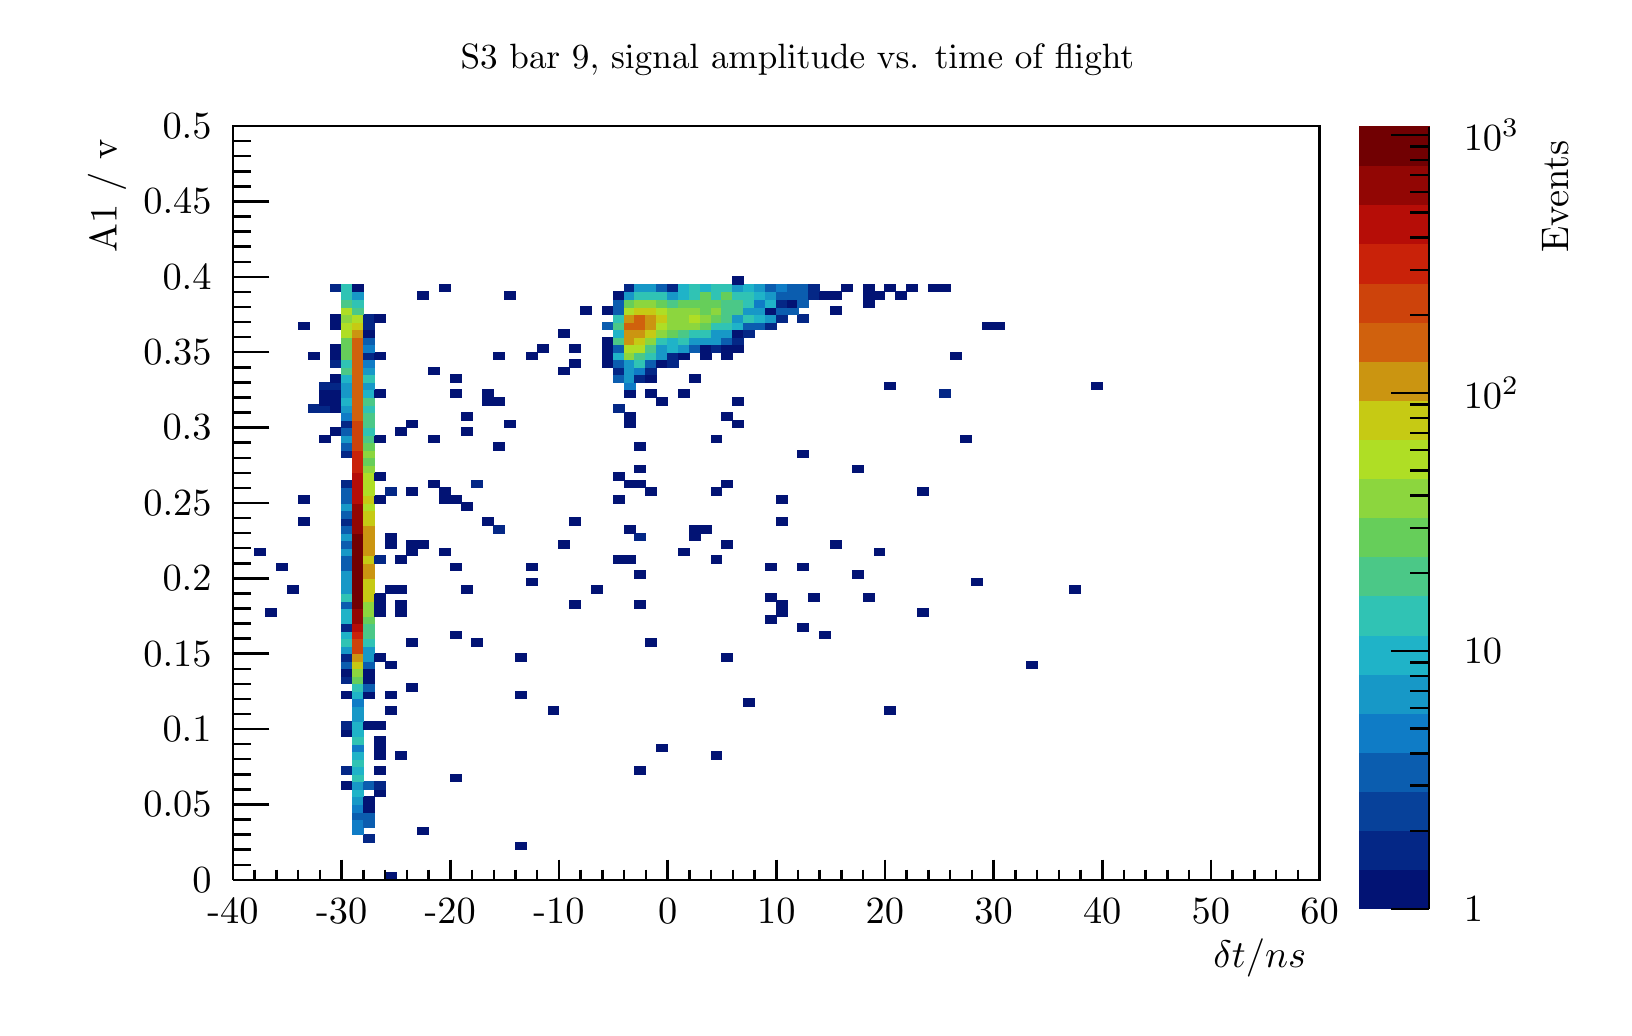
\begin{tikzpicture}
\pgfdeclareplotmark{cross} {
\pgfpathmoveto{\pgfpoint{-0.3\pgfplotmarksize}{\pgfplotmarksize}}
\pgfpathlineto{\pgfpoint{+0.3\pgfplotmarksize}{\pgfplotmarksize}}
\pgfpathlineto{\pgfpoint{+0.3\pgfplotmarksize}{0.3\pgfplotmarksize}}
\pgfpathlineto{\pgfpoint{+1\pgfplotmarksize}{0.3\pgfplotmarksize}}
\pgfpathlineto{\pgfpoint{+1\pgfplotmarksize}{-0.3\pgfplotmarksize}}
\pgfpathlineto{\pgfpoint{+0.3\pgfplotmarksize}{-0.3\pgfplotmarksize}}
\pgfpathlineto{\pgfpoint{+0.3\pgfplotmarksize}{-1.\pgfplotmarksize}}
\pgfpathlineto{\pgfpoint{-0.3\pgfplotmarksize}{-1.\pgfplotmarksize}}
\pgfpathlineto{\pgfpoint{-0.3\pgfplotmarksize}{-0.3\pgfplotmarksize}}
\pgfpathlineto{\pgfpoint{-1.\pgfplotmarksize}{-0.3\pgfplotmarksize}}
\pgfpathlineto{\pgfpoint{-1.\pgfplotmarksize}{0.3\pgfplotmarksize}}
\pgfpathlineto{\pgfpoint{-0.3\pgfplotmarksize}{0.3\pgfplotmarksize}}
\pgfpathclose
\pgfusepathqstroke
}
\pgfdeclareplotmark{cross*} {
\pgfpathmoveto{\pgfpoint{-0.3\pgfplotmarksize}{\pgfplotmarksize}}
\pgfpathlineto{\pgfpoint{+0.3\pgfplotmarksize}{\pgfplotmarksize}}
\pgfpathlineto{\pgfpoint{+0.3\pgfplotmarksize}{0.3\pgfplotmarksize}}
\pgfpathlineto{\pgfpoint{+1\pgfplotmarksize}{0.3\pgfplotmarksize}}
\pgfpathlineto{\pgfpoint{+1\pgfplotmarksize}{-0.3\pgfplotmarksize}}
\pgfpathlineto{\pgfpoint{+0.3\pgfplotmarksize}{-0.3\pgfplotmarksize}}
\pgfpathlineto{\pgfpoint{+0.3\pgfplotmarksize}{-1.\pgfplotmarksize}}
\pgfpathlineto{\pgfpoint{-0.3\pgfplotmarksize}{-1.\pgfplotmarksize}}
\pgfpathlineto{\pgfpoint{-0.3\pgfplotmarksize}{-0.3\pgfplotmarksize}}
\pgfpathlineto{\pgfpoint{-1.\pgfplotmarksize}{-0.3\pgfplotmarksize}}
\pgfpathlineto{\pgfpoint{-1.\pgfplotmarksize}{0.3\pgfplotmarksize}}
\pgfpathlineto{\pgfpoint{-0.3\pgfplotmarksize}{0.3\pgfplotmarksize}}
\pgfpathclose
\pgfusepathqfillstroke
}
\pgfdeclareplotmark{newstar} {
\pgfpathmoveto{\pgfqpoint{0pt}{\pgfplotmarksize}}
\pgfpathlineto{\pgfqpointpolar{44}{0.5\pgfplotmarksize}}
\pgfpathlineto{\pgfqpointpolar{18}{\pgfplotmarksize}}
\pgfpathlineto{\pgfqpointpolar{-20}{0.5\pgfplotmarksize}}
\pgfpathlineto{\pgfqpointpolar{-54}{\pgfplotmarksize}}
\pgfpathlineto{\pgfqpointpolar{-90}{0.5\pgfplotmarksize}}
\pgfpathlineto{\pgfqpointpolar{234}{\pgfplotmarksize}}
\pgfpathlineto{\pgfqpointpolar{198}{0.5\pgfplotmarksize}}
\pgfpathlineto{\pgfqpointpolar{162}{\pgfplotmarksize}}
\pgfpathlineto{\pgfqpointpolar{134}{0.5\pgfplotmarksize}}
\pgfpathclose
\pgfusepathqstroke
}
\pgfdeclareplotmark{newstar*} {
\pgfpathmoveto{\pgfqpoint{0pt}{\pgfplotmarksize}}
\pgfpathlineto{\pgfqpointpolar{44}{0.5\pgfplotmarksize}}
\pgfpathlineto{\pgfqpointpolar{18}{\pgfplotmarksize}}
\pgfpathlineto{\pgfqpointpolar{-20}{0.5\pgfplotmarksize}}
\pgfpathlineto{\pgfqpointpolar{-54}{\pgfplotmarksize}}
\pgfpathlineto{\pgfqpointpolar{-90}{0.5\pgfplotmarksize}}
\pgfpathlineto{\pgfqpointpolar{234}{\pgfplotmarksize}}
\pgfpathlineto{\pgfqpointpolar{198}{0.5\pgfplotmarksize}}
\pgfpathlineto{\pgfqpointpolar{162}{\pgfplotmarksize}}
\pgfpathlineto{\pgfqpointpolar{134}{0.5\pgfplotmarksize}}
\pgfpathclose
\pgfusepathqfillstroke
}
\definecolor{c}{rgb}{1,1,1};
\draw [color=c, fill=c] (0,0) rectangle (20,12.4317);
\draw [color=c, fill=c] (2.6,1.61612) rectangle (16.4,11.1886);
\definecolor{c}{rgb}{0,0,0};
\draw [c,line width=0.9] (2.6,1.61612) -- (2.6,11.1886) -- (16.4,11.1886) -- (16.4,1.61612) -- (2.6,1.61612);
\definecolor{c}{rgb}{1,1,1};
\draw [color=c, fill=c] (2.6,1.61612) rectangle (16.4,11.1886);
\definecolor{c}{rgb}{0,0,0};
\draw [c,line width=0.9] (2.6,1.61612) -- (2.6,11.1886) -- (16.4,11.1886) -- (16.4,1.61612) -- (2.6,1.61612);
\definecolor{c}{rgb}{0.00759013,0.0728653,0.45351};
\draw [color=c, fill=c] (4.532,1.61612) rectangle (4.67,1.71185);
\draw [color=c, fill=c] (6.188,1.99902) rectangle (6.326,2.09475);
\definecolor{c}{rgb}{0.0158128,0.151803,0.524225};
\draw [color=c, fill=c] (4.256,2.09475) rectangle (4.394,2.19047);
\definecolor{c}{rgb}{0.0588235,0.486275,0.776471};
\draw [color=c, fill=c] (4.118,2.19047) rectangle (4.256,2.2862);
\definecolor{c}{rgb}{0.00759013,0.0728653,0.45351};
\draw [color=c, fill=c] (4.946,2.19047) rectangle (5.084,2.2862);
\definecolor{c}{rgb}{0.0588235,0.486275,0.776471};
\draw [color=c, fill=c] (4.118,2.2862) rectangle (4.256,2.38192);
\definecolor{c}{rgb}{0.0428922,0.365196,0.687255};
\draw [color=c, fill=c] (4.256,2.2862) rectangle (4.394,2.38192);
\draw [color=c, fill=c] (4.118,2.38192) rectangle (4.256,2.47764);
\draw [color=c, fill=c] (4.256,2.38192) rectangle (4.394,2.47764);
\definecolor{c}{rgb}{0.0588235,0.486275,0.776471};
\draw [color=c, fill=c] (4.118,2.47764) rectangle (4.256,2.57337);
\definecolor{c}{rgb}{0.00759013,0.0728653,0.45351};
\draw [color=c, fill=c] (4.256,2.47764) rectangle (4.394,2.57337);
\definecolor{c}{rgb}{0.0906863,0.594608,0.78125};
\draw [color=c, fill=c] (4.118,2.57337) rectangle (4.256,2.66909);
\definecolor{c}{rgb}{0.00759013,0.0728653,0.45351};
\draw [color=c, fill=c] (4.256,2.57337) rectangle (4.394,2.66909);
\definecolor{c}{rgb}{0.122549,0.702941,0.786029};
\draw [color=c, fill=c] (4.118,2.66909) rectangle (4.256,2.76482);
\definecolor{c}{rgb}{0.00759013,0.0728653,0.45351};
\draw [color=c, fill=c] (4.394,2.66909) rectangle (4.532,2.76482);
\draw [color=c, fill=c] (3.98,2.76482) rectangle (4.118,2.86054);
\definecolor{c}{rgb}{0.0906863,0.594608,0.78125};
\draw [color=c, fill=c] (4.118,2.76482) rectangle (4.256,2.86054);
\definecolor{c}{rgb}{0.0428922,0.365196,0.687255};
\draw [color=c, fill=c] (4.256,2.76482) rectangle (4.394,2.86054);
\definecolor{c}{rgb}{0.0158128,0.151803,0.524225};
\draw [color=c, fill=c] (4.394,2.76482) rectangle (4.532,2.86054);
\definecolor{c}{rgb}{0.18652,0.763235,0.706618};
\draw [color=c, fill=c] (4.118,2.86054) rectangle (4.256,2.95627);
\definecolor{c}{rgb}{0.00759013,0.0728653,0.45351};
\draw [color=c, fill=c] (5.36,2.86054) rectangle (5.498,2.95627);
\definecolor{c}{rgb}{0.0158128,0.151803,0.524225};
\draw [color=c, fill=c] (3.98,2.95627) rectangle (4.118,3.05199);
\definecolor{c}{rgb}{0.122549,0.702941,0.786029};
\draw [color=c, fill=c] (4.118,2.95627) rectangle (4.256,3.05199);
\definecolor{c}{rgb}{0.00759013,0.0728653,0.45351};
\draw [color=c, fill=c] (4.394,2.95627) rectangle (4.532,3.05199);
\draw [color=c, fill=c] (7.706,2.95627) rectangle (7.844,3.05199);
\definecolor{c}{rgb}{0.18652,0.763235,0.706618};
\draw [color=c, fill=c] (4.118,3.05199) rectangle (4.256,3.14771);
\definecolor{c}{rgb}{0.122549,0.702941,0.786029};
\draw [color=c, fill=c] (4.118,3.14771) rectangle (4.256,3.24344);
\definecolor{c}{rgb}{0.00759013,0.0728653,0.45351};
\draw [color=c, fill=c] (4.394,3.14771) rectangle (4.532,3.24344);
\draw [color=c, fill=c] (4.67,3.14771) rectangle (4.808,3.24344);
\draw [color=c, fill=c] (8.672,3.14771) rectangle (8.81,3.24344);
\definecolor{c}{rgb}{0.0588235,0.486275,0.776471};
\draw [color=c, fill=c] (4.118,3.24344) rectangle (4.256,3.33916);
\definecolor{c}{rgb}{0.00759013,0.0728653,0.45351};
\draw [color=c, fill=c] (4.394,3.24344) rectangle (4.532,3.33916);
\draw [color=c, fill=c] (7.982,3.24344) rectangle (8.12,3.33916);
\definecolor{c}{rgb}{0.18652,0.763235,0.706618};
\draw [color=c, fill=c] (4.118,3.33916) rectangle (4.256,3.43489);
\definecolor{c}{rgb}{0.00759013,0.0728653,0.45351};
\draw [color=c, fill=c] (4.394,3.33916) rectangle (4.532,3.43489);
\draw [color=c, fill=c] (3.98,3.43489) rectangle (4.118,3.53061);
\definecolor{c}{rgb}{0.122549,0.702941,0.786029};
\draw [color=c, fill=c] (4.118,3.43489) rectangle (4.256,3.53061);
\definecolor{c}{rgb}{0.0158128,0.151803,0.524225};
\draw [color=c, fill=c] (3.98,3.53061) rectangle (4.118,3.62634);
\definecolor{c}{rgb}{0.122549,0.702941,0.786029};
\draw [color=c, fill=c] (4.118,3.53061) rectangle (4.256,3.62634);
\definecolor{c}{rgb}{0.00759013,0.0728653,0.45351};
\draw [color=c, fill=c] (4.256,3.53061) rectangle (4.394,3.62634);
\draw [color=c, fill=c] (4.394,3.53061) rectangle (4.532,3.62634);
\definecolor{c}{rgb}{0.0906863,0.594608,0.78125};
\draw [color=c, fill=c] (4.118,3.62634) rectangle (4.256,3.72206);
\draw [color=c, fill=c] (4.118,3.72206) rectangle (4.256,3.81778);
\definecolor{c}{rgb}{0.00759013,0.0728653,0.45351};
\draw [color=c, fill=c] (4.532,3.72206) rectangle (4.67,3.81778);
\draw [color=c, fill=c] (6.602,3.72206) rectangle (6.74,3.81778);
\draw [color=c, fill=c] (10.88,3.72206) rectangle (11.018,3.81778);
\definecolor{c}{rgb}{0.0588235,0.486275,0.776471};
\draw [color=c, fill=c] (4.118,3.81778) rectangle (4.256,3.91351);
\definecolor{c}{rgb}{0.00759013,0.0728653,0.45351};
\draw [color=c, fill=c] (9.086,3.81778) rectangle (9.224,3.91351);
\draw [color=c, fill=c] (3.98,3.91351) rectangle (4.118,4.00923);
\definecolor{c}{rgb}{0.122549,0.702941,0.786029};
\draw [color=c, fill=c] (4.118,3.91351) rectangle (4.256,4.00923);
\definecolor{c}{rgb}{0.00759013,0.0728653,0.45351};
\draw [color=c, fill=c] (4.256,3.91351) rectangle (4.394,4.00923);
\draw [color=c, fill=c] (4.532,3.91351) rectangle (4.67,4.00923);
\draw [color=c, fill=c] (6.188,3.91351) rectangle (6.326,4.00923);
\definecolor{c}{rgb}{0.18652,0.763235,0.706618};
\draw [color=c, fill=c] (4.118,4.00923) rectangle (4.256,4.10496);
\definecolor{c}{rgb}{0.0428922,0.365196,0.687255};
\draw [color=c, fill=c] (4.256,4.00923) rectangle (4.394,4.10496);
\definecolor{c}{rgb}{0.00759013,0.0728653,0.45351};
\draw [color=c, fill=c] (4.808,4.00923) rectangle (4.946,4.10496);
\definecolor{c}{rgb}{0.0158128,0.151803,0.524225};
\draw [color=c, fill=c] (3.98,4.10496) rectangle (4.118,4.20068);
\definecolor{c}{rgb}{0.4,0.807843,0.352941};
\draw [color=c, fill=c] (4.118,4.10496) rectangle (4.256,4.20068);
\definecolor{c}{rgb}{0.00759013,0.0728653,0.45351};
\draw [color=c, fill=c] (4.256,4.10496) rectangle (4.394,4.20068);
\draw [color=c, fill=c] (3.98,4.20068) rectangle (4.118,4.29641);
\definecolor{c}{rgb}{0.549755,0.839706,0.244608};
\draw [color=c, fill=c] (4.118,4.20068) rectangle (4.256,4.29641);
\definecolor{c}{rgb}{0.00759013,0.0728653,0.45351};
\draw [color=c, fill=c] (4.256,4.20068) rectangle (4.394,4.29641);
\definecolor{c}{rgb}{0.0428922,0.365196,0.687255};
\draw [color=c, fill=c] (3.98,4.29641) rectangle (4.118,4.39213);
\definecolor{c}{rgb}{0.777451,0.791422,0.0796569};
\draw [color=c, fill=c] (4.118,4.29641) rectangle (4.256,4.39213);
\definecolor{c}{rgb}{0.0428922,0.365196,0.687255};
\draw [color=c, fill=c] (4.256,4.29641) rectangle (4.394,4.39213);
\definecolor{c}{rgb}{0.00759013,0.0728653,0.45351};
\draw [color=c, fill=c] (4.532,4.29641) rectangle (4.67,4.39213);
\draw [color=c, fill=c] (12.674,4.29641) rectangle (12.812,4.39213);
\definecolor{c}{rgb}{0.0158128,0.151803,0.524225};
\draw [color=c, fill=c] (3.98,4.39213) rectangle (4.118,4.48785);
\definecolor{c}{rgb}{0.796569,0.585907,0.0653186};
\draw [color=c, fill=c] (4.118,4.39213) rectangle (4.256,4.48785);
\definecolor{c}{rgb}{0.0906863,0.594608,0.78125};
\draw [color=c, fill=c] (4.256,4.39213) rectangle (4.394,4.48785);
\definecolor{c}{rgb}{0.00759013,0.0728653,0.45351};
\draw [color=c, fill=c] (4.394,4.39213) rectangle (4.532,4.48785);
\draw [color=c, fill=c] (6.188,4.39213) rectangle (6.326,4.48785);
\draw [color=c, fill=c] (8.81,4.39213) rectangle (8.948,4.48785);
\definecolor{c}{rgb}{0.0906863,0.594608,0.78125};
\draw [color=c, fill=c] (3.98,4.48785) rectangle (4.118,4.58358);
\definecolor{c}{rgb}{0.802451,0.261275,0.0436275};
\draw [color=c, fill=c] (4.118,4.48785) rectangle (4.256,4.58358);
\definecolor{c}{rgb}{0.0906863,0.594608,0.78125};
\draw [color=c, fill=c] (4.256,4.48785) rectangle (4.394,4.58358);
\definecolor{c}{rgb}{0.18652,0.763235,0.706618};
\draw [color=c, fill=c] (3.98,4.58358) rectangle (4.118,4.6793);
\definecolor{c}{rgb}{0.802451,0.261275,0.0436275};
\draw [color=c, fill=c] (4.118,4.58358) rectangle (4.256,4.6793);
\definecolor{c}{rgb}{0.18652,0.763235,0.706618};
\draw [color=c, fill=c] (4.256,4.58358) rectangle (4.394,4.6793);
\definecolor{c}{rgb}{0.00759013,0.0728653,0.45351};
\draw [color=c, fill=c] (4.808,4.58358) rectangle (4.946,4.6793);
\draw [color=c, fill=c] (5.636,4.58358) rectangle (5.774,4.6793);
\draw [color=c, fill=c] (7.844,4.58358) rectangle (7.982,4.6793);
\definecolor{c}{rgb}{0.122549,0.702941,0.786029};
\draw [color=c, fill=c] (3.98,4.6793) rectangle (4.118,4.77503);
\definecolor{c}{rgb}{0.788113,0.13223,0.0356618};
\draw [color=c, fill=c] (4.118,4.6793) rectangle (4.256,4.77503);
\definecolor{c}{rgb}{0.29326,0.785539,0.529779};
\draw [color=c, fill=c] (4.256,4.6793) rectangle (4.394,4.77503);
\definecolor{c}{rgb}{0.00759013,0.0728653,0.45351};
\draw [color=c, fill=c] (5.36,4.6793) rectangle (5.498,4.77503);
\draw [color=c, fill=c] (10.052,4.6793) rectangle (10.19,4.77503);
\definecolor{c}{rgb}{0.0158128,0.151803,0.524225};
\draw [color=c, fill=c] (3.98,4.77503) rectangle (4.118,4.87075);
\definecolor{c}{rgb}{0.714951,0.0509804,0.0269608};
\draw [color=c, fill=c] (4.118,4.77503) rectangle (4.256,4.87075);
\definecolor{c}{rgb}{0.29326,0.785539,0.529779};
\draw [color=c, fill=c] (4.256,4.77503) rectangle (4.394,4.87075);
\definecolor{c}{rgb}{0.00759013,0.0728653,0.45351};
\draw [color=c, fill=c] (9.776,4.77503) rectangle (9.914,4.87075);
\definecolor{c}{rgb}{0.122549,0.702941,0.786029};
\draw [color=c, fill=c] (3.98,4.87075) rectangle (4.118,4.96648);
\definecolor{c}{rgb}{0.573162,0.0254902,0.017402};
\draw [color=c, fill=c] (4.118,4.87075) rectangle (4.256,4.96648);
\definecolor{c}{rgb}{0.4,0.807843,0.352941};
\draw [color=c, fill=c] (4.256,4.87075) rectangle (4.394,4.96648);
\definecolor{c}{rgb}{0.00759013,0.0728653,0.45351};
\draw [color=c, fill=c] (9.362,4.87075) rectangle (9.5,4.96648);
\draw [color=c, fill=c] (3.014,4.96648) rectangle (3.152,5.0622);
\definecolor{c}{rgb}{0.122549,0.702941,0.786029};
\draw [color=c, fill=c] (3.98,4.96648) rectangle (4.118,5.0622);
\definecolor{c}{rgb}{0.573162,0.0254902,0.017402};
\draw [color=c, fill=c] (4.118,4.96648) rectangle (4.256,5.0622);
\definecolor{c}{rgb}{0.549755,0.839706,0.244608};
\draw [color=c, fill=c] (4.256,4.96648) rectangle (4.394,5.0622);
\definecolor{c}{rgb}{0.00759013,0.0728653,0.45351};
\draw [color=c, fill=c] (4.394,4.96648) rectangle (4.532,5.0622);
\draw [color=c, fill=c] (4.67,4.96648) rectangle (4.808,5.0622);
\draw [color=c, fill=c] (9.5,4.96648) rectangle (9.638,5.0622);
\draw [color=c, fill=c] (11.294,4.96648) rectangle (11.432,5.0622);
\definecolor{c}{rgb}{0.0428922,0.365196,0.687255};
\draw [color=c, fill=c] (3.98,5.0622) rectangle (4.118,5.15792);
\definecolor{c}{rgb}{0.442279,0.00196078,0.00857843};
\draw [color=c, fill=c] (4.118,5.0622) rectangle (4.256,5.15792);
\definecolor{c}{rgb}{0.549755,0.839706,0.244608};
\draw [color=c, fill=c] (4.256,5.0622) rectangle (4.394,5.15792);
\definecolor{c}{rgb}{0.00759013,0.0728653,0.45351};
\draw [color=c, fill=c] (4.394,5.0622) rectangle (4.532,5.15792);
\draw [color=c, fill=c] (4.67,5.0622) rectangle (4.808,5.15792);
\draw [color=c, fill=c] (6.878,5.0622) rectangle (7.016,5.15792);
\draw [color=c, fill=c] (7.706,5.0622) rectangle (7.844,5.15792);
\draw [color=c, fill=c] (9.5,5.0622) rectangle (9.638,5.15792);
\definecolor{c}{rgb}{0.18652,0.763235,0.706618};
\draw [color=c, fill=c] (3.98,5.15792) rectangle (4.118,5.25365);
\definecolor{c}{rgb}{0.442279,0.00196078,0.00857843};
\draw [color=c, fill=c] (4.118,5.15792) rectangle (4.256,5.25365);
\definecolor{c}{rgb}{0.777451,0.791422,0.0796569};
\draw [color=c, fill=c] (4.256,5.15792) rectangle (4.394,5.25365);
\definecolor{c}{rgb}{0.00759013,0.0728653,0.45351};
\draw [color=c, fill=c] (4.394,5.15792) rectangle (4.532,5.25365);
\draw [color=c, fill=c] (9.362,5.15792) rectangle (9.5,5.25365);
\draw [color=c, fill=c] (9.914,5.15792) rectangle (10.052,5.25365);
\draw [color=c, fill=c] (10.604,5.15792) rectangle (10.742,5.25365);
\draw [color=c, fill=c] (3.29,5.25365) rectangle (3.428,5.34937);
\definecolor{c}{rgb}{0.0906863,0.594608,0.78125};
\draw [color=c, fill=c] (3.98,5.25365) rectangle (4.118,5.34937);
\definecolor{c}{rgb}{0.442279,0.00196078,0.00857843};
\draw [color=c, fill=c] (4.118,5.25365) rectangle (4.256,5.34937);
\definecolor{c}{rgb}{0.777451,0.791422,0.0796569};
\draw [color=c, fill=c] (4.256,5.25365) rectangle (4.394,5.34937);
\definecolor{c}{rgb}{0.00759013,0.0728653,0.45351};
\draw [color=c, fill=c] (4.532,5.25365) rectangle (4.67,5.34937);
\draw [color=c, fill=c] (4.67,5.25365) rectangle (4.808,5.34937);
\draw [color=c, fill=c] (5.498,5.25365) rectangle (5.636,5.34937);
\draw [color=c, fill=c] (7.154,5.25365) rectangle (7.292,5.34937);
\draw [color=c, fill=c] (13.226,5.25365) rectangle (13.364,5.34937);
\definecolor{c}{rgb}{0.0906863,0.594608,0.78125};
\draw [color=c, fill=c] (3.98,5.34937) rectangle (4.118,5.4451);
\definecolor{c}{rgb}{0.442279,0.00196078,0.00857843};
\draw [color=c, fill=c] (4.118,5.34937) rectangle (4.256,5.4451);
\definecolor{c}{rgb}{0.777451,0.791422,0.0796569};
\draw [color=c, fill=c] (4.256,5.34937) rectangle (4.394,5.4451);
\definecolor{c}{rgb}{0.00759013,0.0728653,0.45351};
\draw [color=c, fill=c] (6.326,5.34937) rectangle (6.464,5.4451);
\draw [color=c, fill=c] (11.984,5.34937) rectangle (12.122,5.4451);
\definecolor{c}{rgb}{0.0906863,0.594608,0.78125};
\draw [color=c, fill=c] (3.98,5.4451) rectangle (4.118,5.54082);
\definecolor{c}{rgb}{0.442279,0.00196078,0.00857843};
\draw [color=c, fill=c] (4.118,5.4451) rectangle (4.256,5.54082);
\definecolor{c}{rgb}{0.796569,0.585907,0.0653186};
\draw [color=c, fill=c] (4.256,5.4451) rectangle (4.394,5.54082);
\definecolor{c}{rgb}{0.00759013,0.0728653,0.45351};
\draw [color=c, fill=c] (7.706,5.4451) rectangle (7.844,5.54082);
\draw [color=c, fill=c] (10.466,5.4451) rectangle (10.604,5.54082);
\draw [color=c, fill=c] (3.152,5.54082) rectangle (3.29,5.63655);
\definecolor{c}{rgb}{0.0428922,0.365196,0.687255};
\draw [color=c, fill=c] (3.98,5.54082) rectangle (4.118,5.63655);
\definecolor{c}{rgb}{0.442279,0.00196078,0.00857843};
\draw [color=c, fill=c] (4.118,5.54082) rectangle (4.256,5.63655);
\definecolor{c}{rgb}{0.796569,0.585907,0.0653186};
\draw [color=c, fill=c] (4.256,5.54082) rectangle (4.394,5.63655);
\definecolor{c}{rgb}{0.00759013,0.0728653,0.45351};
\draw [color=c, fill=c] (5.36,5.54082) rectangle (5.498,5.63655);
\draw [color=c, fill=c] (6.326,5.54082) rectangle (6.464,5.63655);
\draw [color=c, fill=c] (9.362,5.54082) rectangle (9.5,5.63655);
\draw [color=c, fill=c] (9.776,5.54082) rectangle (9.914,5.63655);
\definecolor{c}{rgb}{0.0428922,0.365196,0.687255};
\draw [color=c, fill=c] (3.98,5.63655) rectangle (4.118,5.73227);
\definecolor{c}{rgb}{0.442279,0.00196078,0.00857843};
\draw [color=c, fill=c] (4.118,5.63655) rectangle (4.256,5.73227);
\definecolor{c}{rgb}{0.777451,0.791422,0.0796569};
\draw [color=c, fill=c] (4.256,5.63655) rectangle (4.394,5.73227);
\definecolor{c}{rgb}{0.0158128,0.151803,0.524225};
\draw [color=c, fill=c] (4.394,5.63655) rectangle (4.532,5.73227);
\definecolor{c}{rgb}{0.00759013,0.0728653,0.45351};
\draw [color=c, fill=c] (4.67,5.63655) rectangle (4.808,5.73227);
\draw [color=c, fill=c] (7.43,5.63655) rectangle (7.568,5.73227);
\draw [color=c, fill=c] (7.568,5.63655) rectangle (7.706,5.73227);
\draw [color=c, fill=c] (8.672,5.63655) rectangle (8.81,5.73227);
\draw [color=c, fill=c] (2.876,5.73227) rectangle (3.014,5.82799);
\definecolor{c}{rgb}{0.0906863,0.594608,0.78125};
\draw [color=c, fill=c] (3.98,5.73227) rectangle (4.118,5.82799);
\definecolor{c}{rgb}{0.442279,0.00196078,0.00857843};
\draw [color=c, fill=c] (4.118,5.73227) rectangle (4.256,5.82799);
\definecolor{c}{rgb}{0.796569,0.585907,0.0653186};
\draw [color=c, fill=c] (4.256,5.73227) rectangle (4.394,5.82799);
\definecolor{c}{rgb}{0.00759013,0.0728653,0.45351};
\draw [color=c, fill=c] (4.808,5.73227) rectangle (4.946,5.82799);
\draw [color=c, fill=c] (5.222,5.73227) rectangle (5.36,5.82799);
\draw [color=c, fill=c] (8.258,5.73227) rectangle (8.396,5.82799);
\draw [color=c, fill=c] (10.742,5.73227) rectangle (10.88,5.82799);
\definecolor{c}{rgb}{0.0428922,0.365196,0.687255};
\draw [color=c, fill=c] (3.98,5.82799) rectangle (4.118,5.92372);
\definecolor{c}{rgb}{0.442279,0.00196078,0.00857843};
\draw [color=c, fill=c] (4.118,5.82799) rectangle (4.256,5.92372);
\definecolor{c}{rgb}{0.796569,0.585907,0.0653186};
\draw [color=c, fill=c] (4.256,5.82799) rectangle (4.394,5.92372);
\definecolor{c}{rgb}{0.00759013,0.0728653,0.45351};
\draw [color=c, fill=c] (4.532,5.82799) rectangle (4.67,5.92372);
\draw [color=c, fill=c] (4.808,5.82799) rectangle (4.946,5.92372);
\draw [color=c, fill=c] (4.946,5.82799) rectangle (5.084,5.92372);
\draw [color=c, fill=c] (6.74,5.82799) rectangle (6.878,5.92372);
\draw [color=c, fill=c] (8.81,5.82799) rectangle (8.948,5.92372);
\draw [color=c, fill=c] (10.19,5.82799) rectangle (10.328,5.92372);
\definecolor{c}{rgb}{0.0906863,0.594608,0.78125};
\draw [color=c, fill=c] (3.98,5.92372) rectangle (4.118,6.01944);
\definecolor{c}{rgb}{0.442279,0.00196078,0.00857843};
\draw [color=c, fill=c] (4.118,5.92372) rectangle (4.256,6.01944);
\definecolor{c}{rgb}{0.796569,0.585907,0.0653186};
\draw [color=c, fill=c] (4.256,5.92372) rectangle (4.394,6.01944);
\definecolor{c}{rgb}{0.00759013,0.0728653,0.45351};
\draw [color=c, fill=c] (4.532,5.92372) rectangle (4.67,6.01944);
\definecolor{c}{rgb}{0.0158128,0.151803,0.524225};
\draw [color=c, fill=c] (7.706,5.92372) rectangle (7.844,6.01944);
\definecolor{c}{rgb}{0.00759013,0.0728653,0.45351};
\draw [color=c, fill=c] (8.396,5.92372) rectangle (8.534,6.01944);
\definecolor{c}{rgb}{0.0428922,0.365196,0.687255};
\draw [color=c, fill=c] (3.98,6.01944) rectangle (4.118,6.11517);
\definecolor{c}{rgb}{0.573162,0.0254902,0.017402};
\draw [color=c, fill=c] (4.118,6.01944) rectangle (4.256,6.11517);
\definecolor{c}{rgb}{0.796569,0.585907,0.0653186};
\draw [color=c, fill=c] (4.256,6.01944) rectangle (4.394,6.11517);
\definecolor{c}{rgb}{0.0158128,0.151803,0.524225};
\draw [color=c, fill=c] (5.912,6.01944) rectangle (6.05,6.11517);
\definecolor{c}{rgb}{0.00759013,0.0728653,0.45351};
\draw [color=c, fill=c] (7.568,6.01944) rectangle (7.706,6.11517);
\draw [color=c, fill=c] (8.396,6.01944) rectangle (8.534,6.11517);
\draw [color=c, fill=c] (8.534,6.01944) rectangle (8.672,6.11517);
\draw [color=c, fill=c] (3.428,6.11517) rectangle (3.566,6.21089);
\definecolor{c}{rgb}{0.0158128,0.151803,0.524225};
\draw [color=c, fill=c] (3.98,6.11517) rectangle (4.118,6.21089);
\definecolor{c}{rgb}{0.573162,0.0254902,0.017402};
\draw [color=c, fill=c] (4.118,6.11517) rectangle (4.256,6.21089);
\definecolor{c}{rgb}{0.777451,0.791422,0.0796569};
\draw [color=c, fill=c] (4.256,6.11517) rectangle (4.394,6.21089);
\definecolor{c}{rgb}{0.00759013,0.0728653,0.45351};
\draw [color=c, fill=c] (5.774,6.11517) rectangle (5.912,6.21089);
\draw [color=c, fill=c] (6.878,6.11517) rectangle (7.016,6.21089);
\draw [color=c, fill=c] (9.5,6.11517) rectangle (9.638,6.21089);
\definecolor{c}{rgb}{0.0428922,0.365196,0.687255};
\draw [color=c, fill=c] (3.98,6.21089) rectangle (4.118,6.30662);
\definecolor{c}{rgb}{0.573162,0.0254902,0.017402};
\draw [color=c, fill=c] (4.118,6.21089) rectangle (4.256,6.30662);
\definecolor{c}{rgb}{0.777451,0.791422,0.0796569};
\draw [color=c, fill=c] (4.256,6.21089) rectangle (4.394,6.30662);
\definecolor{c}{rgb}{0.0906863,0.594608,0.78125};
\draw [color=c, fill=c] (3.98,6.30662) rectangle (4.118,6.40234);
\definecolor{c}{rgb}{0.573162,0.0254902,0.017402};
\draw [color=c, fill=c] (4.118,6.30662) rectangle (4.256,6.40234);
\definecolor{c}{rgb}{0.68799,0.869118,0.144608};
\draw [color=c, fill=c] (4.256,6.30662) rectangle (4.394,6.40234);
\definecolor{c}{rgb}{0.00759013,0.0728653,0.45351};
\draw [color=c, fill=c] (5.498,6.30662) rectangle (5.636,6.40234);
\draw [color=c, fill=c] (3.428,6.40234) rectangle (3.566,6.49806);
\definecolor{c}{rgb}{0.0428922,0.365196,0.687255};
\draw [color=c, fill=c] (3.98,6.40234) rectangle (4.118,6.49806);
\definecolor{c}{rgb}{0.714951,0.0509804,0.0269608};
\draw [color=c, fill=c] (4.118,6.40234) rectangle (4.256,6.49806);
\definecolor{c}{rgb}{0.777451,0.791422,0.0796569};
\draw [color=c, fill=c] (4.256,6.40234) rectangle (4.394,6.49806);
\definecolor{c}{rgb}{0.00759013,0.0728653,0.45351};
\draw [color=c, fill=c] (4.394,6.40234) rectangle (4.532,6.49806);
\draw [color=c, fill=c] (5.222,6.40234) rectangle (5.36,6.49806);
\draw [color=c, fill=c] (5.36,6.40234) rectangle (5.498,6.49806);
\draw [color=c, fill=c] (7.43,6.40234) rectangle (7.568,6.49806);
\draw [color=c, fill=c] (9.5,6.40234) rectangle (9.638,6.49806);
\definecolor{c}{rgb}{0.0428922,0.365196,0.687255};
\draw [color=c, fill=c] (3.98,6.49806) rectangle (4.118,6.59379);
\definecolor{c}{rgb}{0.714951,0.0509804,0.0269608};
\draw [color=c, fill=c] (4.118,6.49806) rectangle (4.256,6.59379);
\definecolor{c}{rgb}{0.68799,0.869118,0.144608};
\draw [color=c, fill=c] (4.256,6.49806) rectangle (4.394,6.59379);
\definecolor{c}{rgb}{0.0158128,0.151803,0.524225};
\draw [color=c, fill=c] (4.532,6.49806) rectangle (4.67,6.59379);
\definecolor{c}{rgb}{0.00759013,0.0728653,0.45351};
\draw [color=c, fill=c] (4.808,6.49806) rectangle (4.946,6.59379);
\draw [color=c, fill=c] (5.222,6.49806) rectangle (5.36,6.59379);
\draw [color=c, fill=c] (7.844,6.49806) rectangle (7.982,6.59379);
\draw [color=c, fill=c] (8.672,6.49806) rectangle (8.81,6.59379);
\draw [color=c, fill=c] (11.294,6.49806) rectangle (11.432,6.59379);
\definecolor{c}{rgb}{0.0158128,0.151803,0.524225};
\draw [color=c, fill=c] (3.98,6.59379) rectangle (4.118,6.68951);
\definecolor{c}{rgb}{0.714951,0.0509804,0.0269608};
\draw [color=c, fill=c] (4.118,6.59379) rectangle (4.256,6.68951);
\definecolor{c}{rgb}{0.68799,0.869118,0.144608};
\draw [color=c, fill=c] (4.256,6.59379) rectangle (4.394,6.68951);
\definecolor{c}{rgb}{0.00759013,0.0728653,0.45351};
\draw [color=c, fill=c] (5.084,6.59379) rectangle (5.222,6.68951);
\definecolor{c}{rgb}{0.0158128,0.151803,0.524225};
\draw [color=c, fill=c] (5.636,6.59379) rectangle (5.774,6.68951);
\definecolor{c}{rgb}{0.00759013,0.0728653,0.45351};
\draw [color=c, fill=c] (7.568,6.59379) rectangle (7.706,6.68951);
\draw [color=c, fill=c] (7.706,6.59379) rectangle (7.844,6.68951);
\draw [color=c, fill=c] (8.81,6.59379) rectangle (8.948,6.68951);
\definecolor{c}{rgb}{0.714951,0.0509804,0.0269608};
\draw [color=c, fill=c] (4.118,6.68951) rectangle (4.256,6.78524);
\definecolor{c}{rgb}{0.68799,0.869118,0.144608};
\draw [color=c, fill=c] (4.256,6.68951) rectangle (4.394,6.78524);
\definecolor{c}{rgb}{0.00759013,0.0728653,0.45351};
\draw [color=c, fill=c] (4.394,6.68951) rectangle (4.532,6.78524);
\draw [color=c, fill=c] (7.43,6.68951) rectangle (7.568,6.78524);
\definecolor{c}{rgb}{0.788113,0.13223,0.0356618};
\draw [color=c, fill=c] (4.118,6.78524) rectangle (4.256,6.88096);
\definecolor{c}{rgb}{0.549755,0.839706,0.244608};
\draw [color=c, fill=c] (4.256,6.78524) rectangle (4.394,6.88096);
\definecolor{c}{rgb}{0.00759013,0.0728653,0.45351};
\draw [color=c, fill=c] (7.706,6.78524) rectangle (7.844,6.88096);
\draw [color=c, fill=c] (10.466,6.78524) rectangle (10.604,6.88096);
\definecolor{c}{rgb}{0.788113,0.13223,0.0356618};
\draw [color=c, fill=c] (4.118,6.88096) rectangle (4.256,6.97669);
\definecolor{c}{rgb}{0.4,0.807843,0.352941};
\draw [color=c, fill=c] (4.256,6.88096) rectangle (4.394,6.97669);
\definecolor{c}{rgb}{0.0158128,0.151803,0.524225};
\draw [color=c, fill=c] (3.98,6.97669) rectangle (4.118,7.07241);
\definecolor{c}{rgb}{0.788113,0.13223,0.0356618};
\draw [color=c, fill=c] (4.118,6.97669) rectangle (4.256,7.07241);
\definecolor{c}{rgb}{0.549755,0.839706,0.244608};
\draw [color=c, fill=c] (4.256,6.97669) rectangle (4.394,7.07241);
\definecolor{c}{rgb}{0.00759013,0.0728653,0.45351};
\draw [color=c, fill=c] (9.776,6.97669) rectangle (9.914,7.07241);
\definecolor{c}{rgb}{0.0428922,0.365196,0.687255};
\draw [color=c, fill=c] (3.98,7.07241) rectangle (4.118,7.16814);
\definecolor{c}{rgb}{0.802451,0.261275,0.0436275};
\draw [color=c, fill=c] (4.118,7.07241) rectangle (4.256,7.16814);
\definecolor{c}{rgb}{0.4,0.807843,0.352941};
\draw [color=c, fill=c] (4.256,7.07241) rectangle (4.394,7.16814);
\definecolor{c}{rgb}{0.00759013,0.0728653,0.45351};
\draw [color=c, fill=c] (5.912,7.07241) rectangle (6.05,7.16814);
\draw [color=c, fill=c] (7.706,7.07241) rectangle (7.844,7.16814);
\draw [color=c, fill=c] (3.704,7.16814) rectangle (3.842,7.26386);
\definecolor{c}{rgb}{0.0906863,0.594608,0.78125};
\draw [color=c, fill=c] (3.98,7.16814) rectangle (4.118,7.26386);
\definecolor{c}{rgb}{0.802451,0.261275,0.0436275};
\draw [color=c, fill=c] (4.118,7.16814) rectangle (4.256,7.26386);
\definecolor{c}{rgb}{0.29326,0.785539,0.529779};
\draw [color=c, fill=c] (4.256,7.16814) rectangle (4.394,7.26386);
\definecolor{c}{rgb}{0.00759013,0.0728653,0.45351};
\draw [color=c, fill=c] (4.394,7.16814) rectangle (4.532,7.26386);
\draw [color=c, fill=c] (5.084,7.16814) rectangle (5.222,7.26386);
\draw [color=c, fill=c] (8.672,7.16814) rectangle (8.81,7.26386);
\draw [color=c, fill=c] (11.846,7.16814) rectangle (11.984,7.26386);
\draw [color=c, fill=c] (3.842,7.26386) rectangle (3.98,7.35958);
\definecolor{c}{rgb}{0.0428922,0.365196,0.687255};
\draw [color=c, fill=c] (3.98,7.26386) rectangle (4.118,7.35958);
\definecolor{c}{rgb}{0.802451,0.261275,0.0436275};
\draw [color=c, fill=c] (4.118,7.26386) rectangle (4.256,7.35958);
\definecolor{c}{rgb}{0.18652,0.763235,0.706618};
\draw [color=c, fill=c] (4.256,7.26386) rectangle (4.394,7.35958);
\definecolor{c}{rgb}{0.00759013,0.0728653,0.45351};
\draw [color=c, fill=c] (4.67,7.26386) rectangle (4.808,7.35958);
\draw [color=c, fill=c] (5.498,7.26386) rectangle (5.636,7.35958);
\definecolor{c}{rgb}{0.0158128,0.151803,0.524225};
\draw [color=c, fill=c] (3.98,7.35958) rectangle (4.118,7.45531);
\definecolor{c}{rgb}{0.802451,0.261275,0.0436275};
\draw [color=c, fill=c] (4.118,7.35958) rectangle (4.256,7.45531);
\definecolor{c}{rgb}{0.29326,0.785539,0.529779};
\draw [color=c, fill=c] (4.256,7.35958) rectangle (4.394,7.45531);
\definecolor{c}{rgb}{0.00759013,0.0728653,0.45351};
\draw [color=c, fill=c] (4.808,7.35958) rectangle (4.946,7.45531);
\draw [color=c, fill=c] (6.05,7.35958) rectangle (6.188,7.45531);
\draw [color=c, fill=c] (7.568,7.35958) rectangle (7.706,7.45531);
\draw [color=c, fill=c] (8.948,7.35958) rectangle (9.086,7.45531);
\definecolor{c}{rgb}{0.0588235,0.486275,0.776471};
\draw [color=c, fill=c] (3.98,7.45531) rectangle (4.118,7.55103);
\definecolor{c}{rgb}{0.815686,0.380392,0.0509804};
\draw [color=c, fill=c] (4.118,7.45531) rectangle (4.256,7.55103);
\definecolor{c}{rgb}{0.29326,0.785539,0.529779};
\draw [color=c, fill=c] (4.256,7.45531) rectangle (4.394,7.55103);
\definecolor{c}{rgb}{0.00759013,0.0728653,0.45351};
\draw [color=c, fill=c] (5.498,7.45531) rectangle (5.636,7.55103);
\draw [color=c, fill=c] (7.568,7.45531) rectangle (7.706,7.55103);
\draw [color=c, fill=c] (8.81,7.45531) rectangle (8.948,7.55103);
\definecolor{c}{rgb}{0.0158128,0.151803,0.524225};
\draw [color=c, fill=c] (3.566,7.55103) rectangle (3.704,7.64676);
\draw [color=c, fill=c] (3.704,7.55103) rectangle (3.842,7.64676);
\definecolor{c}{rgb}{0.00759013,0.0728653,0.45351};
\draw [color=c, fill=c] (3.842,7.55103) rectangle (3.98,7.64676);
\definecolor{c}{rgb}{0.0906863,0.594608,0.78125};
\draw [color=c, fill=c] (3.98,7.55103) rectangle (4.118,7.64676);
\definecolor{c}{rgb}{0.815686,0.380392,0.0509804};
\draw [color=c, fill=c] (4.118,7.55103) rectangle (4.256,7.64676);
\definecolor{c}{rgb}{0.18652,0.763235,0.706618};
\draw [color=c, fill=c] (4.256,7.55103) rectangle (4.394,7.64676);
\definecolor{c}{rgb}{0.0158128,0.151803,0.524225};
\draw [color=c, fill=c] (7.43,7.55103) rectangle (7.568,7.64676);
\definecolor{c}{rgb}{0.00759013,0.0728653,0.45351};
\draw [color=c, fill=c] (3.704,7.64676) rectangle (3.842,7.74248);
\draw [color=c, fill=c] (3.842,7.64676) rectangle (3.98,7.74248);
\definecolor{c}{rgb}{0.122549,0.702941,0.786029};
\draw [color=c, fill=c] (3.98,7.64676) rectangle (4.118,7.74248);
\definecolor{c}{rgb}{0.815686,0.380392,0.0509804};
\draw [color=c, fill=c] (4.118,7.64676) rectangle (4.256,7.74248);
\definecolor{c}{rgb}{0.29326,0.785539,0.529779};
\draw [color=c, fill=c] (4.256,7.64676) rectangle (4.394,7.74248);
\definecolor{c}{rgb}{0.00759013,0.0728653,0.45351};
\draw [color=c, fill=c] (5.774,7.64676) rectangle (5.912,7.74248);
\draw [color=c, fill=c] (5.912,7.64676) rectangle (6.05,7.74248);
\draw [color=c, fill=c] (7.982,7.64676) rectangle (8.12,7.74248);
\draw [color=c, fill=c] (8.948,7.64676) rectangle (9.086,7.74248);
\draw [color=c, fill=c] (3.704,7.74248) rectangle (3.842,7.83821);
\draw [color=c, fill=c] (3.842,7.74248) rectangle (3.98,7.83821);
\definecolor{c}{rgb}{0.0906863,0.594608,0.78125};
\draw [color=c, fill=c] (3.98,7.74248) rectangle (4.118,7.83821);
\definecolor{c}{rgb}{0.815686,0.380392,0.0509804};
\draw [color=c, fill=c] (4.118,7.74248) rectangle (4.256,7.83821);
\definecolor{c}{rgb}{0.122549,0.702941,0.786029};
\draw [color=c, fill=c] (4.256,7.74248) rectangle (4.394,7.83821);
\definecolor{c}{rgb}{0.00759013,0.0728653,0.45351};
\draw [color=c, fill=c] (4.394,7.74248) rectangle (4.532,7.83821);
\draw [color=c, fill=c] (5.36,7.74248) rectangle (5.498,7.83821);
\draw [color=c, fill=c] (5.774,7.74248) rectangle (5.912,7.83821);
\draw [color=c, fill=c] (7.568,7.74248) rectangle (7.706,7.83821);
\draw [color=c, fill=c] (7.844,7.74248) rectangle (7.982,7.83821);
\draw [color=c, fill=c] (8.258,7.74248) rectangle (8.396,7.83821);
\definecolor{c}{rgb}{0.0158128,0.151803,0.524225};
\draw [color=c, fill=c] (11.57,7.74248) rectangle (11.708,7.83821);
\draw [color=c, fill=c] (3.704,7.83821) rectangle (3.842,7.93393);
\draw [color=c, fill=c] (3.842,7.83821) rectangle (3.98,7.93393);
\definecolor{c}{rgb}{0.0906863,0.594608,0.78125};
\draw [color=c, fill=c] (3.98,7.83821) rectangle (4.118,7.93393);
\definecolor{c}{rgb}{0.815686,0.380392,0.0509804};
\draw [color=c, fill=c] (4.118,7.83821) rectangle (4.256,7.93393);
\definecolor{c}{rgb}{0.0906863,0.594608,0.78125};
\draw [color=c, fill=c] (4.256,7.83821) rectangle (4.394,7.93393);
\definecolor{c}{rgb}{0.0588235,0.486275,0.776471};
\draw [color=c, fill=c] (7.568,7.83821) rectangle (7.706,7.93393);
\definecolor{c}{rgb}{0.00759013,0.0728653,0.45351};
\draw [color=c, fill=c] (10.88,7.83821) rectangle (11.018,7.93393);
\draw [color=c, fill=c] (13.502,7.83821) rectangle (13.64,7.93393);
\draw [color=c, fill=c] (3.842,7.93393) rectangle (3.98,8.02965);
\definecolor{c}{rgb}{0.122549,0.702941,0.786029};
\draw [color=c, fill=c] (3.98,7.93393) rectangle (4.118,8.02965);
\definecolor{c}{rgb}{0.815686,0.380392,0.0509804};
\draw [color=c, fill=c] (4.118,7.93393) rectangle (4.256,8.02965);
\definecolor{c}{rgb}{0.18652,0.763235,0.706618};
\draw [color=c, fill=c] (4.256,7.93393) rectangle (4.394,8.02965);
\definecolor{c}{rgb}{0.00759013,0.0728653,0.45351};
\draw [color=c, fill=c] (5.36,7.93393) rectangle (5.498,8.02965);
\definecolor{c}{rgb}{0.0428922,0.365196,0.687255};
\draw [color=c, fill=c] (7.43,7.93393) rectangle (7.568,8.02965);
\definecolor{c}{rgb}{0.0906863,0.594608,0.78125};
\draw [color=c, fill=c] (7.568,7.93393) rectangle (7.706,8.02965);
\definecolor{c}{rgb}{0.0158128,0.151803,0.524225};
\draw [color=c, fill=c] (7.706,7.93393) rectangle (7.844,8.02965);
\definecolor{c}{rgb}{0.00759013,0.0728653,0.45351};
\draw [color=c, fill=c] (7.844,7.93393) rectangle (7.982,8.02965);
\draw [color=c, fill=c] (8.396,7.93393) rectangle (8.534,8.02965);
\definecolor{c}{rgb}{0.29326,0.785539,0.529779};
\draw [color=c, fill=c] (3.98,8.02965) rectangle (4.118,8.12538);
\definecolor{c}{rgb}{0.815686,0.380392,0.0509804};
\draw [color=c, fill=c] (4.118,8.02965) rectangle (4.256,8.12538);
\definecolor{c}{rgb}{0.0906863,0.594608,0.78125};
\draw [color=c, fill=c] (4.256,8.02965) rectangle (4.394,8.12538);
\definecolor{c}{rgb}{0.00759013,0.0728653,0.45351};
\draw [color=c, fill=c] (5.084,8.02965) rectangle (5.222,8.12538);
\draw [color=c, fill=c] (6.74,8.02965) rectangle (6.878,8.12538);
\definecolor{c}{rgb}{0.0158128,0.151803,0.524225};
\draw [color=c, fill=c] (7.43,8.02965) rectangle (7.568,8.12538);
\definecolor{c}{rgb}{0.0906863,0.594608,0.78125};
\draw [color=c, fill=c] (7.568,8.02965) rectangle (7.706,8.12538);
\definecolor{c}{rgb}{0.0588235,0.486275,0.776471};
\draw [color=c, fill=c] (7.706,8.02965) rectangle (7.844,8.12538);
\definecolor{c}{rgb}{0.0158128,0.151803,0.524225};
\draw [color=c, fill=c] (7.844,8.02965) rectangle (7.982,8.12538);
\draw [color=c, fill=c] (3.842,8.12538) rectangle (3.98,8.2211);
\definecolor{c}{rgb}{0.18652,0.763235,0.706618};
\draw [color=c, fill=c] (3.98,8.12538) rectangle (4.118,8.2211);
\definecolor{c}{rgb}{0.815686,0.380392,0.0509804};
\draw [color=c, fill=c] (4.118,8.12538) rectangle (4.256,8.2211);
\definecolor{c}{rgb}{0.0588235,0.486275,0.776471};
\draw [color=c, fill=c] (4.256,8.12538) rectangle (4.394,8.2211);
\definecolor{c}{rgb}{0.00759013,0.0728653,0.45351};
\draw [color=c, fill=c] (6.878,8.12538) rectangle (7.016,8.2211);
\draw [color=c, fill=c] (7.292,8.12538) rectangle (7.43,8.2211);
\definecolor{c}{rgb}{0.0428922,0.365196,0.687255};
\draw [color=c, fill=c] (7.43,8.12538) rectangle (7.568,8.2211);
\definecolor{c}{rgb}{0.0906863,0.594608,0.78125};
\draw [color=c, fill=c] (7.568,8.12538) rectangle (7.706,8.2211);
\definecolor{c}{rgb}{0.18652,0.763235,0.706618};
\draw [color=c, fill=c] (7.706,8.12538) rectangle (7.844,8.2211);
\definecolor{c}{rgb}{0.0428922,0.365196,0.687255};
\draw [color=c, fill=c] (7.844,8.12538) rectangle (7.982,8.2211);
\definecolor{c}{rgb}{0.00759013,0.0728653,0.45351};
\draw [color=c, fill=c] (7.982,8.12538) rectangle (8.12,8.2211);
\definecolor{c}{rgb}{0.0158128,0.151803,0.524225};
\draw [color=c, fill=c] (8.12,8.12538) rectangle (8.258,8.2211);
\definecolor{c}{rgb}{0.00759013,0.0728653,0.45351};
\draw [color=c, fill=c] (3.566,8.2211) rectangle (3.704,8.31683);
\draw [color=c, fill=c] (3.842,8.2211) rectangle (3.98,8.31683);
\definecolor{c}{rgb}{0.4,0.807843,0.352941};
\draw [color=c, fill=c] (3.98,8.2211) rectangle (4.118,8.31683);
\definecolor{c}{rgb}{0.815686,0.380392,0.0509804};
\draw [color=c, fill=c] (4.118,8.2211) rectangle (4.256,8.31683);
\definecolor{c}{rgb}{0.0158128,0.151803,0.524225};
\draw [color=c, fill=c] (4.256,8.2211) rectangle (4.394,8.31683);
\definecolor{c}{rgb}{0.00759013,0.0728653,0.45351};
\draw [color=c, fill=c] (4.394,8.2211) rectangle (4.532,8.31683);
\draw [color=c, fill=c] (5.912,8.2211) rectangle (6.05,8.31683);
\draw [color=c, fill=c] (6.326,8.2211) rectangle (6.464,8.31683);
\draw [color=c, fill=c] (7.292,8.2211) rectangle (7.43,8.31683);
\definecolor{c}{rgb}{0.122549,0.702941,0.786029};
\draw [color=c, fill=c] (7.43,8.2211) rectangle (7.568,8.31683);
\definecolor{c}{rgb}{0.549755,0.839706,0.244608};
\draw [color=c, fill=c] (7.568,8.2211) rectangle (7.706,8.31683);
\definecolor{c}{rgb}{0.29326,0.785539,0.529779};
\draw [color=c, fill=c] (7.706,8.2211) rectangle (7.844,8.31683);
\definecolor{c}{rgb}{0.18652,0.763235,0.706618};
\draw [color=c, fill=c] (7.844,8.2211) rectangle (7.982,8.31683);
\definecolor{c}{rgb}{0.0906863,0.594608,0.78125};
\draw [color=c, fill=c] (7.982,8.2211) rectangle (8.12,8.31683);
\definecolor{c}{rgb}{0.0158128,0.151803,0.524225};
\draw [color=c, fill=c] (8.12,8.2211) rectangle (8.258,8.31683);
\definecolor{c}{rgb}{0.00759013,0.0728653,0.45351};
\draw [color=c, fill=c] (8.258,8.2211) rectangle (8.396,8.31683);
\draw [color=c, fill=c] (8.534,8.2211) rectangle (8.672,8.31683);
\draw [color=c, fill=c] (8.81,8.2211) rectangle (8.948,8.31683);
\draw [color=c, fill=c] (11.708,8.2211) rectangle (11.846,8.31683);
\draw [color=c, fill=c] (3.842,8.31683) rectangle (3.98,8.41255);
\definecolor{c}{rgb}{0.4,0.807843,0.352941};
\draw [color=c, fill=c] (3.98,8.31683) rectangle (4.118,8.41255);
\definecolor{c}{rgb}{0.815686,0.380392,0.0509804};
\draw [color=c, fill=c] (4.118,8.31683) rectangle (4.256,8.41255);
\definecolor{c}{rgb}{0.0588235,0.486275,0.776471};
\draw [color=c, fill=c] (4.256,8.31683) rectangle (4.394,8.41255);
\definecolor{c}{rgb}{0.00759013,0.0728653,0.45351};
\draw [color=c, fill=c] (6.464,8.31683) rectangle (6.602,8.41255);
\draw [color=c, fill=c] (6.878,8.31683) rectangle (7.016,8.41255);
\draw [color=c, fill=c] (7.292,8.31683) rectangle (7.43,8.41255);
\definecolor{c}{rgb}{0.0428922,0.365196,0.687255};
\draw [color=c, fill=c] (7.43,8.31683) rectangle (7.568,8.41255);
\definecolor{c}{rgb}{0.68799,0.869118,0.144608};
\draw [color=c, fill=c] (7.568,8.31683) rectangle (7.706,8.41255);
\draw [color=c, fill=c] (7.706,8.31683) rectangle (7.844,8.41255);
\definecolor{c}{rgb}{0.29326,0.785539,0.529779};
\draw [color=c, fill=c] (7.844,8.31683) rectangle (7.982,8.41255);
\definecolor{c}{rgb}{0.0906863,0.594608,0.78125};
\draw [color=c, fill=c] (7.982,8.31683) rectangle (8.12,8.41255);
\definecolor{c}{rgb}{0.122549,0.702941,0.786029};
\draw [color=c, fill=c] (8.12,8.31683) rectangle (8.258,8.41255);
\definecolor{c}{rgb}{0.0906863,0.594608,0.78125};
\draw [color=c, fill=c] (8.258,8.31683) rectangle (8.396,8.41255);
\definecolor{c}{rgb}{0.0428922,0.365196,0.687255};
\draw [color=c, fill=c] (8.396,8.31683) rectangle (8.534,8.41255);
\definecolor{c}{rgb}{0.00759013,0.0728653,0.45351};
\draw [color=c, fill=c] (8.534,8.31683) rectangle (8.672,8.41255);
\definecolor{c}{rgb}{0.0158128,0.151803,0.524225};
\draw [color=c, fill=c] (8.672,8.31683) rectangle (8.81,8.41255);
\definecolor{c}{rgb}{0.00759013,0.0728653,0.45351};
\draw [color=c, fill=c] (8.81,8.31683) rectangle (8.948,8.41255);
\draw [color=c, fill=c] (8.948,8.31683) rectangle (9.086,8.41255);
\definecolor{c}{rgb}{0.4,0.807843,0.352941};
\draw [color=c, fill=c] (3.98,8.41255) rectangle (4.118,8.50828);
\definecolor{c}{rgb}{0.815686,0.380392,0.0509804};
\draw [color=c, fill=c] (4.118,8.41255) rectangle (4.256,8.50828);
\definecolor{c}{rgb}{0.0428922,0.365196,0.687255};
\draw [color=c, fill=c] (4.256,8.41255) rectangle (4.394,8.50828);
\definecolor{c}{rgb}{0.00759013,0.0728653,0.45351};
\draw [color=c, fill=c] (7.292,8.41255) rectangle (7.43,8.50828);
\definecolor{c}{rgb}{0.29326,0.785539,0.529779};
\draw [color=c, fill=c] (7.43,8.41255) rectangle (7.568,8.50828);
\definecolor{c}{rgb}{0.796569,0.585907,0.0653186};
\draw [color=c, fill=c] (7.568,8.41255) rectangle (7.706,8.50828);
\definecolor{c}{rgb}{0.777451,0.791422,0.0796569};
\draw [color=c, fill=c] (7.706,8.41255) rectangle (7.844,8.50828);
\definecolor{c}{rgb}{0.549755,0.839706,0.244608};
\draw [color=c, fill=c] (7.844,8.41255) rectangle (7.982,8.50828);
\definecolor{c}{rgb}{0.18652,0.763235,0.706618};
\draw [color=c, fill=c] (7.982,8.41255) rectangle (8.12,8.50828);
\definecolor{c}{rgb}{0.122549,0.702941,0.786029};
\draw [color=c, fill=c] (8.12,8.41255) rectangle (8.258,8.50828);
\definecolor{c}{rgb}{0.18652,0.763235,0.706618};
\draw [color=c, fill=c] (8.258,8.41255) rectangle (8.396,8.50828);
\definecolor{c}{rgb}{0.0906863,0.594608,0.78125};
\draw [color=c, fill=c] (8.396,8.41255) rectangle (8.534,8.50828);
\draw [color=c, fill=c] (8.534,8.41255) rectangle (8.672,8.50828);
\draw [color=c, fill=c] (8.672,8.41255) rectangle (8.81,8.50828);
\definecolor{c}{rgb}{0.0428922,0.365196,0.687255};
\draw [color=c, fill=c] (8.81,8.41255) rectangle (8.948,8.50828);
\definecolor{c}{rgb}{0.0158128,0.151803,0.524225};
\draw [color=c, fill=c] (8.948,8.41255) rectangle (9.086,8.50828);
\definecolor{c}{rgb}{0.68799,0.869118,0.144608};
\draw [color=c, fill=c] (3.98,8.50828) rectangle (4.118,8.604);
\definecolor{c}{rgb}{0.796569,0.585907,0.0653186};
\draw [color=c, fill=c] (4.118,8.50828) rectangle (4.256,8.604);
\definecolor{c}{rgb}{0.00759013,0.0728653,0.45351};
\draw [color=c, fill=c] (4.256,8.50828) rectangle (4.394,8.604);
\draw [color=c, fill=c] (6.74,8.50828) rectangle (6.878,8.604);
\definecolor{c}{rgb}{0.122549,0.702941,0.786029};
\draw [color=c, fill=c] (7.43,8.50828) rectangle (7.568,8.604);
\definecolor{c}{rgb}{0.796569,0.585907,0.0653186};
\draw [color=c, fill=c] (7.568,8.50828) rectangle (7.706,8.604);
\draw [color=c, fill=c] (7.706,8.50828) rectangle (7.844,8.604);
\definecolor{c}{rgb}{0.777451,0.791422,0.0796569};
\draw [color=c, fill=c] (7.844,8.50828) rectangle (7.982,8.604);
\definecolor{c}{rgb}{0.549755,0.839706,0.244608};
\draw [color=c, fill=c] (7.982,8.50828) rectangle (8.12,8.604);
\definecolor{c}{rgb}{0.4,0.807843,0.352941};
\draw [color=c, fill=c] (8.12,8.50828) rectangle (8.258,8.604);
\definecolor{c}{rgb}{0.29326,0.785539,0.529779};
\draw [color=c, fill=c] (8.258,8.50828) rectangle (8.396,8.604);
\definecolor{c}{rgb}{0.18652,0.763235,0.706618};
\draw [color=c, fill=c] (8.396,8.50828) rectangle (8.534,8.604);
\draw [color=c, fill=c] (8.534,8.50828) rectangle (8.672,8.604);
\definecolor{c}{rgb}{0.0906863,0.594608,0.78125};
\draw [color=c, fill=c] (8.672,8.50828) rectangle (8.81,8.604);
\draw [color=c, fill=c] (8.81,8.50828) rectangle (8.948,8.604);
\definecolor{c}{rgb}{0.00759013,0.0728653,0.45351};
\draw [color=c, fill=c] (8.948,8.50828) rectangle (9.086,8.604);
\definecolor{c}{rgb}{0.0158128,0.151803,0.524225};
\draw [color=c, fill=c] (9.086,8.50828) rectangle (9.224,8.604);
\definecolor{c}{rgb}{0.00759013,0.0728653,0.45351};
\draw [color=c, fill=c] (3.428,8.604) rectangle (3.566,8.69972);
\draw [color=c, fill=c] (3.842,8.604) rectangle (3.98,8.69972);
\definecolor{c}{rgb}{0.68799,0.869118,0.144608};
\draw [color=c, fill=c] (3.98,8.604) rectangle (4.118,8.69972);
\definecolor{c}{rgb}{0.777451,0.791422,0.0796569};
\draw [color=c, fill=c] (4.118,8.604) rectangle (4.256,8.69972);
\definecolor{c}{rgb}{0.0158128,0.151803,0.524225};
\draw [color=c, fill=c] (4.256,8.604) rectangle (4.394,8.69972);
\definecolor{c}{rgb}{0.0428922,0.365196,0.687255};
\draw [color=c, fill=c] (7.292,8.604) rectangle (7.43,8.69972);
\definecolor{c}{rgb}{0.29326,0.785539,0.529779};
\draw [color=c, fill=c] (7.43,8.604) rectangle (7.568,8.69972);
\definecolor{c}{rgb}{0.815686,0.380392,0.0509804};
\draw [color=c, fill=c] (7.568,8.604) rectangle (7.706,8.69972);
\draw [color=c, fill=c] (7.706,8.604) rectangle (7.844,8.69972);
\definecolor{c}{rgb}{0.796569,0.585907,0.0653186};
\draw [color=c, fill=c] (7.844,8.604) rectangle (7.982,8.69972);
\definecolor{c}{rgb}{0.68799,0.869118,0.144608};
\draw [color=c, fill=c] (7.982,8.604) rectangle (8.12,8.69972);
\definecolor{c}{rgb}{0.549755,0.839706,0.244608};
\draw [color=c, fill=c] (8.12,8.604) rectangle (8.258,8.69972);
\draw [color=c, fill=c] (8.258,8.604) rectangle (8.396,8.69972);
\draw [color=c, fill=c] (8.396,8.604) rectangle (8.534,8.69972);
\definecolor{c}{rgb}{0.4,0.807843,0.352941};
\draw [color=c, fill=c] (8.534,8.604) rectangle (8.672,8.69972);
\definecolor{c}{rgb}{0.18652,0.763235,0.706618};
\draw [color=c, fill=c] (8.672,8.604) rectangle (8.81,8.69972);
\draw [color=c, fill=c] (8.81,8.604) rectangle (8.948,8.69972);
\definecolor{c}{rgb}{0.122549,0.702941,0.786029};
\draw [color=c, fill=c] (8.948,8.604) rectangle (9.086,8.69972);
\definecolor{c}{rgb}{0.0428922,0.365196,0.687255};
\draw [color=c, fill=c] (9.086,8.604) rectangle (9.224,8.69972);
\draw [color=c, fill=c] (9.224,8.604) rectangle (9.362,8.69972);
\definecolor{c}{rgb}{0.0158128,0.151803,0.524225};
\draw [color=c, fill=c] (9.362,8.604) rectangle (9.5,8.69972);
\definecolor{c}{rgb}{0.00759013,0.0728653,0.45351};
\draw [color=c, fill=c] (12.122,8.604) rectangle (12.26,8.69972);
\draw [color=c, fill=c] (12.26,8.604) rectangle (12.398,8.69972);
\draw [color=c, fill=c] (3.842,8.69972) rectangle (3.98,8.79545);
\definecolor{c}{rgb}{0.549755,0.839706,0.244608};
\draw [color=c, fill=c] (3.98,8.69972) rectangle (4.118,8.79545);
\definecolor{c}{rgb}{0.68799,0.869118,0.144608};
\draw [color=c, fill=c] (4.118,8.69972) rectangle (4.256,8.79545);
\definecolor{c}{rgb}{0.0158128,0.151803,0.524225};
\draw [color=c, fill=c] (4.256,8.69972) rectangle (4.394,8.79545);
\definecolor{c}{rgb}{0.00759013,0.0728653,0.45351};
\draw [color=c, fill=c] (4.394,8.69972) rectangle (4.532,8.79545);
\definecolor{c}{rgb}{0.18652,0.763235,0.706618};
\draw [color=c, fill=c] (7.43,8.69972) rectangle (7.568,8.79545);
\definecolor{c}{rgb}{0.796569,0.585907,0.0653186};
\draw [color=c, fill=c] (7.568,8.69972) rectangle (7.706,8.79545);
\definecolor{c}{rgb}{0.815686,0.380392,0.0509804};
\draw [color=c, fill=c] (7.706,8.69972) rectangle (7.844,8.79545);
\definecolor{c}{rgb}{0.796569,0.585907,0.0653186};
\draw [color=c, fill=c] (7.844,8.69972) rectangle (7.982,8.79545);
\definecolor{c}{rgb}{0.777451,0.791422,0.0796569};
\draw [color=c, fill=c] (7.982,8.69972) rectangle (8.12,8.79545);
\definecolor{c}{rgb}{0.549755,0.839706,0.244608};
\draw [color=c, fill=c] (8.12,8.69972) rectangle (8.258,8.79545);
\draw [color=c, fill=c] (8.258,8.69972) rectangle (8.396,8.79545);
\definecolor{c}{rgb}{0.68799,0.869118,0.144608};
\draw [color=c, fill=c] (8.396,8.69972) rectangle (8.534,8.79545);
\definecolor{c}{rgb}{0.549755,0.839706,0.244608};
\draw [color=c, fill=c] (8.534,8.69972) rectangle (8.672,8.79545);
\definecolor{c}{rgb}{0.4,0.807843,0.352941};
\draw [color=c, fill=c] (8.672,8.69972) rectangle (8.81,8.79545);
\definecolor{c}{rgb}{0.29326,0.785539,0.529779};
\draw [color=c, fill=c] (8.81,8.69972) rectangle (8.948,8.79545);
\definecolor{c}{rgb}{0.0906863,0.594608,0.78125};
\draw [color=c, fill=c] (8.948,8.69972) rectangle (9.086,8.79545);
\definecolor{c}{rgb}{0.18652,0.763235,0.706618};
\draw [color=c, fill=c] (9.086,8.69972) rectangle (9.224,8.79545);
\definecolor{c}{rgb}{0.122549,0.702941,0.786029};
\draw [color=c, fill=c] (9.224,8.69972) rectangle (9.362,8.79545);
\definecolor{c}{rgb}{0.0906863,0.594608,0.78125};
\draw [color=c, fill=c] (9.362,8.69972) rectangle (9.5,8.79545);
\definecolor{c}{rgb}{0.0158128,0.151803,0.524225};
\draw [color=c, fill=c] (9.5,8.69972) rectangle (9.638,8.79545);
\draw [color=c, fill=c] (9.776,8.69972) rectangle (9.914,8.79545);
\definecolor{c}{rgb}{0.68799,0.869118,0.144608};
\draw [color=c, fill=c] (3.98,8.79545) rectangle (4.118,8.89117);
\definecolor{c}{rgb}{0.29326,0.785539,0.529779};
\draw [color=c, fill=c] (4.118,8.79545) rectangle (4.256,8.89117);
\definecolor{c}{rgb}{0.00759013,0.0728653,0.45351};
\draw [color=c, fill=c] (7.016,8.79545) rectangle (7.154,8.89117);
\draw [color=c, fill=c] (7.292,8.79545) rectangle (7.43,8.89117);
\definecolor{c}{rgb}{0.0428922,0.365196,0.687255};
\draw [color=c, fill=c] (7.43,8.79545) rectangle (7.568,8.89117);
\definecolor{c}{rgb}{0.68799,0.869118,0.144608};
\draw [color=c, fill=c] (7.568,8.79545) rectangle (7.706,8.89117);
\definecolor{c}{rgb}{0.777451,0.791422,0.0796569};
\draw [color=c, fill=c] (7.706,8.79545) rectangle (7.844,8.89117);
\draw [color=c, fill=c] (7.844,8.79545) rectangle (7.982,8.89117);
\definecolor{c}{rgb}{0.68799,0.869118,0.144608};
\draw [color=c, fill=c] (7.982,8.79545) rectangle (8.12,8.89117);
\definecolor{c}{rgb}{0.549755,0.839706,0.244608};
\draw [color=c, fill=c] (8.12,8.79545) rectangle (8.258,8.89117);
\draw [color=c, fill=c] (8.258,8.79545) rectangle (8.396,8.89117);
\draw [color=c, fill=c] (8.396,8.79545) rectangle (8.534,8.89117);
\definecolor{c}{rgb}{0.4,0.807843,0.352941};
\draw [color=c, fill=c] (8.534,8.79545) rectangle (8.672,8.89117);
\definecolor{c}{rgb}{0.549755,0.839706,0.244608};
\draw [color=c, fill=c] (8.672,8.79545) rectangle (8.81,8.89117);
\definecolor{c}{rgb}{0.29326,0.785539,0.529779};
\draw [color=c, fill=c] (8.81,8.79545) rectangle (8.948,8.89117);
\draw [color=c, fill=c] (8.948,8.79545) rectangle (9.086,8.89117);
\definecolor{c}{rgb}{0.0906863,0.594608,0.78125};
\draw [color=c, fill=c] (9.086,8.79545) rectangle (9.224,8.89117);
\draw [color=c, fill=c] (9.224,8.79545) rectangle (9.362,8.89117);
\definecolor{c}{rgb}{0.00759013,0.0728653,0.45351};
\draw [color=c, fill=c] (9.362,8.79545) rectangle (9.5,8.89117);
\definecolor{c}{rgb}{0.0428922,0.365196,0.687255};
\draw [color=c, fill=c] (9.5,8.79545) rectangle (9.638,8.89117);
\draw [color=c, fill=c] (9.638,8.79545) rectangle (9.776,8.89117);
\definecolor{c}{rgb}{0.00759013,0.0728653,0.45351};
\draw [color=c, fill=c] (10.19,8.79545) rectangle (10.328,8.89117);
\definecolor{c}{rgb}{0.29326,0.785539,0.529779};
\draw [color=c, fill=c] (3.98,8.89117) rectangle (4.118,8.9869);
\definecolor{c}{rgb}{0.18652,0.763235,0.706618};
\draw [color=c, fill=c] (4.118,8.89117) rectangle (4.256,8.9869);
\definecolor{c}{rgb}{0.0428922,0.365196,0.687255};
\draw [color=c, fill=c] (7.43,8.89117) rectangle (7.568,8.9869);
\definecolor{c}{rgb}{0.4,0.807843,0.352941};
\draw [color=c, fill=c] (7.568,8.89117) rectangle (7.706,8.9869);
\definecolor{c}{rgb}{0.549755,0.839706,0.244608};
\draw [color=c, fill=c] (7.706,8.89117) rectangle (7.844,8.9869);
\draw [color=c, fill=c] (7.844,8.89117) rectangle (7.982,8.9869);
\definecolor{c}{rgb}{0.4,0.807843,0.352941};
\draw [color=c, fill=c] (7.982,8.89117) rectangle (8.12,8.9869);
\definecolor{c}{rgb}{0.29326,0.785539,0.529779};
\draw [color=c, fill=c] (8.12,8.89117) rectangle (8.258,8.9869);
\definecolor{c}{rgb}{0.4,0.807843,0.352941};
\draw [color=c, fill=c] (8.258,8.89117) rectangle (8.396,8.9869);
\draw [color=c, fill=c] (8.396,8.89117) rectangle (8.534,8.9869);
\draw [color=c, fill=c] (8.534,8.89117) rectangle (8.672,8.9869);
\draw [color=c, fill=c] (8.672,8.89117) rectangle (8.81,8.9869);
\definecolor{c}{rgb}{0.29326,0.785539,0.529779};
\draw [color=c, fill=c] (8.81,8.89117) rectangle (8.948,8.9869);
\draw [color=c, fill=c] (8.948,8.89117) rectangle (9.086,8.9869);
\definecolor{c}{rgb}{0.18652,0.763235,0.706618};
\draw [color=c, fill=c] (9.086,8.89117) rectangle (9.224,8.9869);
\definecolor{c}{rgb}{0.0588235,0.486275,0.776471};
\draw [color=c, fill=c] (9.224,8.89117) rectangle (9.362,8.9869);
\definecolor{c}{rgb}{0.122549,0.702941,0.786029};
\draw [color=c, fill=c] (9.362,8.89117) rectangle (9.5,8.9869);
\definecolor{c}{rgb}{0.0158128,0.151803,0.524225};
\draw [color=c, fill=c] (9.5,8.89117) rectangle (9.638,8.9869);
\definecolor{c}{rgb}{0.00759013,0.0728653,0.45351};
\draw [color=c, fill=c] (9.638,8.89117) rectangle (9.776,8.9869);
\definecolor{c}{rgb}{0.0428922,0.365196,0.687255};
\draw [color=c, fill=c] (9.776,8.89117) rectangle (9.914,8.9869);
\definecolor{c}{rgb}{0.00759013,0.0728653,0.45351};
\draw [color=c, fill=c] (10.604,8.89117) rectangle (10.742,8.9869);
\definecolor{c}{rgb}{0.18652,0.763235,0.706618};
\draw [color=c, fill=c] (3.98,8.9869) rectangle (4.118,9.08262);
\definecolor{c}{rgb}{0.0906863,0.594608,0.78125};
\draw [color=c, fill=c] (4.118,8.9869) rectangle (4.256,9.08262);
\definecolor{c}{rgb}{0.00759013,0.0728653,0.45351};
\draw [color=c, fill=c] (4.946,8.9869) rectangle (5.084,9.08262);
\draw [color=c, fill=c] (6.05,8.9869) rectangle (6.188,9.08262);
\draw [color=c, fill=c] (7.43,8.9869) rectangle (7.568,9.08262);
\definecolor{c}{rgb}{0.0906863,0.594608,0.78125};
\draw [color=c, fill=c] (7.568,8.9869) rectangle (7.706,9.08262);
\definecolor{c}{rgb}{0.18652,0.763235,0.706618};
\draw [color=c, fill=c] (7.706,8.9869) rectangle (7.844,9.08262);
\draw [color=c, fill=c] (7.844,8.9869) rectangle (7.982,9.08262);
\draw [color=c, fill=c] (7.982,8.9869) rectangle (8.12,9.08262);
\definecolor{c}{rgb}{0.0906863,0.594608,0.78125};
\draw [color=c, fill=c] (8.12,8.9869) rectangle (8.258,9.08262);
\definecolor{c}{rgb}{0.122549,0.702941,0.786029};
\draw [color=c, fill=c] (8.258,8.9869) rectangle (8.396,9.08262);
\definecolor{c}{rgb}{0.18652,0.763235,0.706618};
\draw [color=c, fill=c] (8.396,8.9869) rectangle (8.534,9.08262);
\definecolor{c}{rgb}{0.4,0.807843,0.352941};
\draw [color=c, fill=c] (8.534,8.9869) rectangle (8.672,9.08262);
\definecolor{c}{rgb}{0.18652,0.763235,0.706618};
\draw [color=c, fill=c] (8.672,8.9869) rectangle (8.81,9.08262);
\definecolor{c}{rgb}{0.4,0.807843,0.352941};
\draw [color=c, fill=c] (8.81,8.9869) rectangle (8.948,9.08262);
\definecolor{c}{rgb}{0.18652,0.763235,0.706618};
\draw [color=c, fill=c] (8.948,8.9869) rectangle (9.086,9.08262);
\draw [color=c, fill=c] (9.086,8.9869) rectangle (9.224,9.08262);
\definecolor{c}{rgb}{0.122549,0.702941,0.786029};
\draw [color=c, fill=c] (9.224,8.9869) rectangle (9.362,9.08262);
\definecolor{c}{rgb}{0.0906863,0.594608,0.78125};
\draw [color=c, fill=c] (9.362,8.9869) rectangle (9.5,9.08262);
\definecolor{c}{rgb}{0.0428922,0.365196,0.687255};
\draw [color=c, fill=c] (9.5,8.9869) rectangle (9.638,9.08262);
\draw [color=c, fill=c] (9.638,8.9869) rectangle (9.776,9.08262);
\draw [color=c, fill=c] (9.776,8.9869) rectangle (9.914,9.08262);
\definecolor{c}{rgb}{0.0158128,0.151803,0.524225};
\draw [color=c, fill=c] (9.914,8.9869) rectangle (10.052,9.08262);
\definecolor{c}{rgb}{0.00759013,0.0728653,0.45351};
\draw [color=c, fill=c] (10.052,8.9869) rectangle (10.19,9.08262);
\draw [color=c, fill=c] (10.19,8.9869) rectangle (10.328,9.08262);
\draw [color=c, fill=c] (10.604,8.9869) rectangle (10.742,9.08262);
\draw [color=c, fill=c] (10.742,8.9869) rectangle (10.88,9.08262);
\draw [color=c, fill=c] (11.018,8.9869) rectangle (11.156,9.08262);
\definecolor{c}{rgb}{0.0158128,0.151803,0.524225};
\draw [color=c, fill=c] (3.842,9.08262) rectangle (3.98,9.17835);
\definecolor{c}{rgb}{0.18652,0.763235,0.706618};
\draw [color=c, fill=c] (3.98,9.08262) rectangle (4.118,9.17835);
\definecolor{c}{rgb}{0.00759013,0.0728653,0.45351};
\draw [color=c, fill=c] (4.118,9.08262) rectangle (4.256,9.17835);
\draw [color=c, fill=c] (5.222,9.08262) rectangle (5.36,9.17835);
\definecolor{c}{rgb}{0.0158128,0.151803,0.524225};
\draw [color=c, fill=c] (7.568,9.08262) rectangle (7.706,9.17835);
\definecolor{c}{rgb}{0.0906863,0.594608,0.78125};
\draw [color=c, fill=c] (7.706,9.08262) rectangle (7.844,9.17835);
\draw [color=c, fill=c] (7.844,9.08262) rectangle (7.982,9.17835);
\definecolor{c}{rgb}{0.0428922,0.365196,0.687255};
\draw [color=c, fill=c] (7.982,9.08262) rectangle (8.12,9.17835);
\definecolor{c}{rgb}{0.0158128,0.151803,0.524225};
\draw [color=c, fill=c] (8.12,9.08262) rectangle (8.258,9.17835);
\definecolor{c}{rgb}{0.122549,0.702941,0.786029};
\draw [color=c, fill=c] (8.258,9.08262) rectangle (8.396,9.17835);
\definecolor{c}{rgb}{0.18652,0.763235,0.706618};
\draw [color=c, fill=c] (8.396,9.08262) rectangle (8.534,9.17835);
\definecolor{c}{rgb}{0.122549,0.702941,0.786029};
\draw [color=c, fill=c] (8.534,9.08262) rectangle (8.672,9.17835);
\definecolor{c}{rgb}{0.18652,0.763235,0.706618};
\draw [color=c, fill=c] (8.672,9.08262) rectangle (8.81,9.17835);
\draw [color=c, fill=c] (8.81,9.08262) rectangle (8.948,9.17835);
\definecolor{c}{rgb}{0.0906863,0.594608,0.78125};
\draw [color=c, fill=c] (8.948,9.08262) rectangle (9.086,9.17835);
\definecolor{c}{rgb}{0.122549,0.702941,0.786029};
\draw [color=c, fill=c] (9.086,9.08262) rectangle (9.224,9.17835);
\definecolor{c}{rgb}{0.0906863,0.594608,0.78125};
\draw [color=c, fill=c] (9.224,9.08262) rectangle (9.362,9.17835);
\definecolor{c}{rgb}{0.0428922,0.365196,0.687255};
\draw [color=c, fill=c] (9.362,9.08262) rectangle (9.5,9.17835);
\definecolor{c}{rgb}{0.0588235,0.486275,0.776471};
\draw [color=c, fill=c] (9.5,9.08262) rectangle (9.638,9.17835);
\definecolor{c}{rgb}{0.0428922,0.365196,0.687255};
\draw [color=c, fill=c] (9.638,9.08262) rectangle (9.776,9.17835);
\draw [color=c, fill=c] (9.776,9.08262) rectangle (9.914,9.17835);
\definecolor{c}{rgb}{0.0158128,0.151803,0.524225};
\draw [color=c, fill=c] (9.914,9.08262) rectangle (10.052,9.17835);
\definecolor{c}{rgb}{0.00759013,0.0728653,0.45351};
\draw [color=c, fill=c] (10.328,9.08262) rectangle (10.466,9.17835);
\draw [color=c, fill=c] (10.604,9.08262) rectangle (10.742,9.17835);
\draw [color=c, fill=c] (10.88,9.08262) rectangle (11.018,9.17835);
\draw [color=c, fill=c] (11.156,9.08262) rectangle (11.294,9.17835);
\draw [color=c, fill=c] (11.432,9.08262) rectangle (11.57,9.17835);
\draw [color=c, fill=c] (11.57,9.08262) rectangle (11.708,9.17835);
\draw [color=c, fill=c] (8.948,9.17835) rectangle (9.086,9.27407);
\definecolor{c}{rgb}{0,0,0};
\draw [c,line width=0.9] (2.6,1.61612) -- (16.4,1.61612);
\draw [c,line width=0.9] (2.6,1.87346) -- (2.6,1.61612);
\draw [c,line width=0.9] (2.876,1.74479) -- (2.876,1.61612);
\draw [c,line width=0.9] (3.152,1.74479) -- (3.152,1.61612);
\draw [c,line width=0.9] (3.428,1.74479) -- (3.428,1.61612);
\draw [c,line width=0.9] (3.704,1.74479) -- (3.704,1.61612);
\draw [c,line width=0.9] (3.98,1.87346) -- (3.98,1.61612);
\draw [c,line width=0.9] (4.256,1.74479) -- (4.256,1.61612);
\draw [c,line width=0.9] (4.532,1.74479) -- (4.532,1.61612);
\draw [c,line width=0.9] (4.808,1.74479) -- (4.808,1.61612);
\draw [c,line width=0.9] (5.084,1.74479) -- (5.084,1.61612);
\draw [c,line width=0.9] (5.36,1.87346) -- (5.36,1.61612);
\draw [c,line width=0.9] (5.636,1.74479) -- (5.636,1.61612);
\draw [c,line width=0.9] (5.912,1.74479) -- (5.912,1.61612);
\draw [c,line width=0.9] (6.188,1.74479) -- (6.188,1.61612);
\draw [c,line width=0.9] (6.464,1.74479) -- (6.464,1.61612);
\draw [c,line width=0.9] (6.74,1.87346) -- (6.74,1.61612);
\draw [c,line width=0.9] (7.016,1.74479) -- (7.016,1.61612);
\draw [c,line width=0.9] (7.292,1.74479) -- (7.292,1.61612);
\draw [c,line width=0.9] (7.568,1.74479) -- (7.568,1.61612);
\draw [c,line width=0.9] (7.844,1.74479) -- (7.844,1.61612);
\draw [c,line width=0.9] (8.12,1.87346) -- (8.12,1.61612);
\draw [c,line width=0.9] (8.396,1.74479) -- (8.396,1.61612);
\draw [c,line width=0.9] (8.672,1.74479) -- (8.672,1.61612);
\draw [c,line width=0.9] (8.948,1.74479) -- (8.948,1.61612);
\draw [c,line width=0.9] (9.224,1.74479) -- (9.224,1.61612);
\draw [c,line width=0.9] (9.5,1.87346) -- (9.5,1.61612);
\draw [c,line width=0.9] (9.776,1.74479) -- (9.776,1.61612);
\draw [c,line width=0.9] (10.052,1.74479) -- (10.052,1.61612);
\draw [c,line width=0.9] (10.328,1.74479) -- (10.328,1.61612);
\draw [c,line width=0.9] (10.604,1.74479) -- (10.604,1.61612);
\draw [c,line width=0.9] (10.88,1.87346) -- (10.88,1.61612);
\draw [c,line width=0.9] (11.156,1.74479) -- (11.156,1.61612);
\draw [c,line width=0.9] (11.432,1.74479) -- (11.432,1.61612);
\draw [c,line width=0.9] (11.708,1.74479) -- (11.708,1.61612);
\draw [c,line width=0.9] (11.984,1.74479) -- (11.984,1.61612);
\draw [c,line width=0.9] (12.26,1.87346) -- (12.26,1.61612);
\draw [c,line width=0.9] (12.536,1.74479) -- (12.536,1.61612);
\draw [c,line width=0.9] (12.812,1.74479) -- (12.812,1.61612);
\draw [c,line width=0.9] (13.088,1.74479) -- (13.088,1.61612);
\draw [c,line width=0.9] (13.364,1.74479) -- (13.364,1.61612);
\draw [c,line width=0.9] (13.64,1.87346) -- (13.64,1.61612);
\draw [c,line width=0.9] (13.916,1.74479) -- (13.916,1.61612);
\draw [c,line width=0.9] (14.192,1.74479) -- (14.192,1.61612);
\draw [c,line width=0.9] (14.468,1.74479) -- (14.468,1.61612);
\draw [c,line width=0.9] (14.744,1.74479) -- (14.744,1.61612);
\draw [c,line width=0.9] (15.02,1.87346) -- (15.02,1.61612);
\draw [c,line width=0.9] (15.296,1.74479) -- (15.296,1.61612);
\draw [c,line width=0.9] (15.572,1.74479) -- (15.572,1.61612);
\draw [c,line width=0.9] (15.848,1.74479) -- (15.848,1.61612);
\draw [c,line width=0.9] (16.124,1.74479) -- (16.124,1.61612);
\draw [c,line width=0.9] (16.4,1.87346) -- (16.4,1.61612);
\draw [anchor=base] (2.6,1.0567) node[scale=1.3863, color=c, rotate=0]{-40};
\draw [anchor=base] (3.98,1.0567) node[scale=1.3863, color=c, rotate=0]{-30};
\draw [anchor=base] (5.36,1.0567) node[scale=1.3863, color=c, rotate=0]{-20};
\draw [anchor=base] (6.74,1.0567) node[scale=1.3863, color=c, rotate=0]{-10};
\draw [anchor=base] (8.12,1.0567) node[scale=1.3863, color=c, rotate=0]{0};
\draw [anchor=base] (9.5,1.0567) node[scale=1.3863, color=c, rotate=0]{10};
\draw [anchor=base] (10.88,1.0567) node[scale=1.3863, color=c, rotate=0]{20};
\draw [anchor=base] (12.26,1.0567) node[scale=1.3863, color=c, rotate=0]{30};
\draw [anchor=base] (13.64,1.0567) node[scale=1.3863, color=c, rotate=0]{40};
\draw [anchor=base] (15.02,1.0567) node[scale=1.3863, color=c, rotate=0]{50};
\draw [anchor=base] (16.4,1.0567) node[scale=1.3863, color=c, rotate=0]{60};
\draw [anchor= east] (16.4,0.621586) node[scale=1.3863, color=c, rotate=0]{$ \delta t / ns$};
\draw [c,line width=0.9] (2.6,1.61612) -- (2.6,11.1886);
\draw [c,line width=0.9] (3.062,1.61612) -- (2.6,1.61612);
\draw [c,line width=0.9] (2.831,1.80757) -- (2.6,1.80757);
\draw [c,line width=0.9] (2.831,1.99902) -- (2.6,1.99902);
\draw [c,line width=0.9] (2.831,2.19047) -- (2.6,2.19047);
\draw [c,line width=0.9] (2.831,2.38192) -- (2.6,2.38192);
\draw [c,line width=0.9] (3.062,2.57337) -- (2.6,2.57337);
\draw [c,line width=0.9] (2.831,2.76482) -- (2.6,2.76482);
\draw [c,line width=0.9] (2.831,2.95627) -- (2.6,2.95627);
\draw [c,line width=0.9] (2.831,3.14771) -- (2.6,3.14771);
\draw [c,line width=0.9] (2.831,3.33916) -- (2.6,3.33916);
\draw [c,line width=0.9] (3.062,3.53061) -- (2.6,3.53061);
\draw [c,line width=0.9] (2.831,3.72206) -- (2.6,3.72206);
\draw [c,line width=0.9] (2.831,3.91351) -- (2.6,3.91351);
\draw [c,line width=0.9] (2.831,4.10496) -- (2.6,4.10496);
\draw [c,line width=0.9] (2.831,4.29641) -- (2.6,4.29641);
\draw [c,line width=0.9] (3.062,4.48785) -- (2.6,4.48785);
\draw [c,line width=0.9] (2.831,4.6793) -- (2.6,4.6793);
\draw [c,line width=0.9] (2.831,4.87075) -- (2.6,4.87075);
\draw [c,line width=0.9] (2.831,5.0622) -- (2.6,5.0622);
\draw [c,line width=0.9] (2.831,5.25365) -- (2.6,5.25365);
\draw [c,line width=0.9] (3.062,5.4451) -- (2.6,5.4451);
\draw [c,line width=0.9] (2.831,5.63655) -- (2.6,5.63655);
\draw [c,line width=0.9] (2.831,5.82799) -- (2.6,5.82799);
\draw [c,line width=0.9] (2.831,6.01944) -- (2.6,6.01944);
\draw [c,line width=0.9] (2.831,6.21089) -- (2.6,6.21089);
\draw [c,line width=0.9] (3.062,6.40234) -- (2.6,6.40234);
\draw [c,line width=0.9] (2.831,6.59379) -- (2.6,6.59379);
\draw [c,line width=0.9] (2.831,6.78524) -- (2.6,6.78524);
\draw [c,line width=0.9] (2.831,6.97669) -- (2.6,6.97669);
\draw [c,line width=0.9] (2.831,7.16814) -- (2.6,7.16814);
\draw [c,line width=0.9] (3.062,7.35958) -- (2.6,7.35958);
\draw [c,line width=0.9] (2.831,7.55103) -- (2.6,7.55103);
\draw [c,line width=0.9] (2.831,7.74248) -- (2.6,7.74248);
\draw [c,line width=0.9] (2.831,7.93393) -- (2.6,7.93393);
\draw [c,line width=0.9] (2.831,8.12538) -- (2.6,8.12538);
\draw [c,line width=0.9] (3.062,8.31683) -- (2.6,8.31683);
\draw [c,line width=0.9] (2.831,8.50828) -- (2.6,8.50828);
\draw [c,line width=0.9] (2.831,8.69972) -- (2.6,8.69972);
\draw [c,line width=0.9] (2.831,8.89117) -- (2.6,8.89117);
\draw [c,line width=0.9] (2.831,9.08262) -- (2.6,9.08262);
\draw [c,line width=0.9] (3.062,9.27407) -- (2.6,9.27407);
\draw [c,line width=0.9] (2.831,9.46552) -- (2.6,9.46552);
\draw [c,line width=0.9] (2.831,9.65697) -- (2.6,9.65697);
\draw [c,line width=0.9] (2.831,9.84842) -- (2.6,9.84842);
\draw [c,line width=0.9] (2.831,10.0399) -- (2.6,10.0399);
\draw [c,line width=0.9] (3.062,10.2313) -- (2.6,10.2313);
\draw [c,line width=0.9] (2.831,10.4228) -- (2.6,10.4228);
\draw [c,line width=0.9] (2.831,10.6142) -- (2.6,10.6142);
\draw [c,line width=0.9] (2.831,10.8057) -- (2.6,10.8057);
\draw [c,line width=0.9] (2.831,10.9971) -- (2.6,10.9971);
\draw [c,line width=0.9] (3.062,11.1886) -- (2.6,11.1886);
\draw [anchor= east] (2.5,1.61612) node[scale=1.3863, color=c, rotate=0]{0};
\draw [anchor= east] (2.5,2.57337) node[scale=1.3863, color=c, rotate=0]{0.05};
\draw [anchor= east] (2.5,3.53061) node[scale=1.3863, color=c, rotate=0]{0.1};
\draw [anchor= east] (2.5,4.48785) node[scale=1.3863, color=c, rotate=0]{0.15};
\draw [anchor= east] (2.5,5.4451) node[scale=1.3863, color=c, rotate=0]{0.2};
\draw [anchor= east] (2.5,6.40234) node[scale=1.3863, color=c, rotate=0]{0.25};
\draw [anchor= east] (2.5,7.35958) node[scale=1.3863, color=c, rotate=0]{0.3};
\draw [anchor= east] (2.5,8.31683) node[scale=1.3863, color=c, rotate=0]{0.35};
\draw [anchor= east] (2.5,9.27407) node[scale=1.3863, color=c, rotate=0]{0.4};
\draw [anchor= east] (2.5,10.2313) node[scale=1.3863, color=c, rotate=0]{0.45};
\draw [anchor= east] (2.5,11.1886) node[scale=1.3863, color=c, rotate=0]{0.5};
\draw [anchor= east] (1,11.1886) node[scale=1.3863, color=c, rotate=90]{ A1 / v};
\definecolor{c}{rgb}{0.00759013,0.0728653,0.45351};
\draw [color=c, fill=c] (16.9051,1.24837) rectangle (17.7893,1.74512);
\definecolor{c}{rgb}{0.0158128,0.151803,0.524225};
\draw [color=c, fill=c] (16.9051,1.74512) rectangle (17.7893,2.24187);
\definecolor{c}{rgb}{0.0281863,0.253431,0.604902};
\draw [color=c, fill=c] (16.9051,2.24187) rectangle (17.7893,2.73862);
\definecolor{c}{rgb}{0.0428922,0.365196,0.687255};
\draw [color=c, fill=c] (16.9051,2.73862) rectangle (17.7893,3.23537);
\definecolor{c}{rgb}{0.0588235,0.486275,0.776471};
\draw [color=c, fill=c] (16.9051,3.23537) rectangle (17.7893,3.73212);
\definecolor{c}{rgb}{0.0906863,0.594608,0.78125};
\draw [color=c, fill=c] (16.9051,3.73212) rectangle (17.7893,4.22887);
\definecolor{c}{rgb}{0.122549,0.702941,0.786029};
\draw [color=c, fill=c] (16.9051,4.22887) rectangle (17.7893,4.72562);
\definecolor{c}{rgb}{0.18652,0.763235,0.706618};
\draw [color=c, fill=c] (16.9051,4.72562) rectangle (17.7893,5.22237);
\definecolor{c}{rgb}{0.29326,0.785539,0.529779};
\draw [color=c, fill=c] (16.9051,5.22237) rectangle (17.7893,5.71912);
\definecolor{c}{rgb}{0.4,0.807843,0.352941};
\draw [color=c, fill=c] (16.9051,5.71912) rectangle (17.7893,6.21586);
\definecolor{c}{rgb}{0.549755,0.839706,0.244608};
\draw [color=c, fill=c] (16.9051,6.21586) rectangle (17.7893,6.71261);
\definecolor{c}{rgb}{0.68799,0.869118,0.144608};
\draw [color=c, fill=c] (16.9051,6.71261) rectangle (17.7893,7.20936);
\definecolor{c}{rgb}{0.777451,0.791422,0.0796569};
\draw [color=c, fill=c] (16.9051,7.20936) rectangle (17.7893,7.70611);
\definecolor{c}{rgb}{0.796569,0.585907,0.0653186};
\draw [color=c, fill=c] (16.9051,7.70611) rectangle (17.7893,8.20286);
\definecolor{c}{rgb}{0.815686,0.380392,0.0509804};
\draw [color=c, fill=c] (16.9051,8.20286) rectangle (17.7893,8.69961);
\definecolor{c}{rgb}{0.802451,0.261275,0.0436275};
\draw [color=c, fill=c] (16.9051,8.69961) rectangle (17.7893,9.19636);
\definecolor{c}{rgb}{0.788113,0.13223,0.0356618};
\draw [color=c, fill=c] (16.9051,9.19636) rectangle (17.7893,9.69311);
\definecolor{c}{rgb}{0.714951,0.0509804,0.0269608};
\draw [color=c, fill=c] (16.9051,9.69311) rectangle (17.7893,10.1899);
\definecolor{c}{rgb}{0.573162,0.0254902,0.017402};
\draw [color=c, fill=c] (16.9051,10.1899) rectangle (17.7893,10.6866);
\definecolor{c}{rgb}{0.442279,0.00196078,0.00857843};
\draw [color=c, fill=c] (16.9051,10.6866) rectangle (17.7893,11.1834);
\definecolor{c}{rgb}{0,0,0};
\draw [c,line width=0.9] (17.7893,1.24837) -- (17.7893,11.1834);
\draw [c,line width=0.9] (17.3098,1.24838) -- (17.7893,1.24838);
\draw [anchor= west] (18.0593,1.24838) node[scale=1.3863, color=c, rotate=0]{1};
\draw [c,line width=0.9] (17.5496,2.23456) -- (17.7893,2.23456);
\draw [c,line width=0.9] (17.5496,2.81145) -- (17.7893,2.81145);
\draw [c,line width=0.9] (17.5496,3.22075) -- (17.7893,3.22075);
\draw [c,line width=0.9] (17.5496,3.53823) -- (17.7893,3.53823);
\draw [c,line width=0.9] (17.5496,3.79763) -- (17.7893,3.79763);
\draw [c,line width=0.9] (17.5496,4.01695) -- (17.7893,4.01695);
\draw [c,line width=0.9] (17.5496,4.20694) -- (17.7893,4.20694);
\draw [c,line width=0.9] (17.5496,4.37451) -- (17.7893,4.37451);
\draw [c,line width=0.9] (17.3098,4.52442) -- (17.7893,4.52442);
\draw [anchor= west] (18.0593,4.52442) node[scale=1.3863, color=c, rotate=0]{10};
\draw [c,line width=0.9] (17.5496,5.5106) -- (17.7893,5.5106);
\draw [c,line width=0.9] (17.5496,6.08748) -- (17.7893,6.08748);
\draw [c,line width=0.9] (17.5496,6.49679) -- (17.7893,6.49679);
\draw [c,line width=0.9] (17.5496,6.81427) -- (17.7893,6.81427);
\draw [c,line width=0.9] (17.5496,7.07367) -- (17.7893,7.07367);
\draw [c,line width=0.9] (17.5496,7.29299) -- (17.7893,7.29299);
\draw [c,line width=0.9] (17.5496,7.48297) -- (17.7893,7.48297);
\draw [c,line width=0.9] (17.5496,7.65055) -- (17.7893,7.65055);
\draw [c,line width=0.9] (17.3098,7.80046) -- (17.7893,7.80046);
\draw [anchor= west] (18.0593,7.80046) node[scale=1.3863, color=c, rotate=0]{$10^{2}$};
\draw [c,line width=0.9] (17.5496,8.78664) -- (17.7893,8.78664);
\draw [c,line width=0.9] (17.5496,9.36352) -- (17.7893,9.36352);
\draw [c,line width=0.9] (17.5496,9.77283) -- (17.7893,9.77283);
\draw [c,line width=0.9] (17.5496,10.0903) -- (17.7893,10.0903);
\draw [c,line width=0.9] (17.5496,10.3497) -- (17.7893,10.3497);
\draw [c,line width=0.9] (17.5496,10.569) -- (17.7893,10.569);
\draw [c,line width=0.9] (17.5496,10.759) -- (17.7893,10.759);
\draw [c,line width=0.9] (17.5496,10.9266) -- (17.7893,10.9266);
\draw [c,line width=0.9] (17.3098,11.0765) -- (17.7893,11.0765);
\draw [anchor= west] (18.0593,11.0765) node[scale=1.3863, color=c, rotate=0]{$10^{3}$};
\draw [anchor= east] (19.3893,11.1834) node[scale=1.3863, color=c, rotate=90]{ Events};
\draw (9.76712,12.0375) node[scale=1.27078, color=c, rotate=0]{S3 bar 9, signal amplitude vs. time of flight};
\end{tikzpicture}

		\end{adjustbox}
		\caption{Example of SiPM signal amplitude plotted against uncorrected $S3$ time of flight. The population in the upper right is thought to be produced by protons.}
		\label{fig:TvsA}
	\end{figure}
	